\documentclass[twoside]{book}

% Packages required by doxygen
\usepackage{fixltx2e}
\usepackage{calc}
\usepackage{doxygen}
\usepackage[export]{adjustbox} % also loads graphicx
\usepackage{graphicx}
\usepackage[utf8]{inputenc}
\usepackage{makeidx}
\usepackage{multicol}
\usepackage{multirow}
\PassOptionsToPackage{warn}{textcomp}
\usepackage{textcomp}
\usepackage[nointegrals]{wasysym}
\usepackage[table]{xcolor}

% Font selection
\usepackage[T1]{fontenc}
\usepackage[scaled=.90]{helvet}
\usepackage{courier}
\usepackage{amssymb}
\usepackage{sectsty}
\renewcommand{\familydefault}{\sfdefault}
\allsectionsfont{%
  \fontseries{bc}\selectfont%
  \color{darkgray}%
}
\renewcommand{\DoxyLabelFont}{%
  \fontseries{bc}\selectfont%
  \color{darkgray}%
}
\newcommand{\+}{\discretionary{\mbox{\scriptsize$\hookleftarrow$}}{}{}}

% Page & text layout
\usepackage{geometry}
\geometry{%
  a4paper,%
  top=2.5cm,%
  bottom=2.5cm,%
  left=2.5cm,%
  right=2.5cm%
}
\tolerance=750
\hfuzz=15pt
\hbadness=750
\setlength{\emergencystretch}{15pt}
\setlength{\parindent}{0cm}
\setlength{\parskip}{3ex plus 2ex minus 2ex}
\makeatletter
\renewcommand{\paragraph}{%
  \@startsection{paragraph}{4}{0ex}{-1.0ex}{1.0ex}{%
    \normalfont\normalsize\bfseries\SS@parafont%
  }%
}
\renewcommand{\subparagraph}{%
  \@startsection{subparagraph}{5}{0ex}{-1.0ex}{1.0ex}{%
    \normalfont\normalsize\bfseries\SS@subparafont%
  }%
}
\makeatother

% Headers & footers
\usepackage{fancyhdr}
\pagestyle{fancyplain}
\fancyhead[LE]{\fancyplain{}{\bfseries\thepage}}
\fancyhead[CE]{\fancyplain{}{}}
\fancyhead[RE]{\fancyplain{}{\bfseries\leftmark}}
\fancyhead[LO]{\fancyplain{}{\bfseries\rightmark}}
\fancyhead[CO]{\fancyplain{}{}}
\fancyhead[RO]{\fancyplain{}{\bfseries\thepage}}
\fancyfoot[LE]{\fancyplain{}{}}
\fancyfoot[CE]{\fancyplain{}{}}
\fancyfoot[RE]{\fancyplain{}{\bfseries\scriptsize Generated by Doxygen }}
\fancyfoot[LO]{\fancyplain{}{\bfseries\scriptsize Generated by Doxygen }}
\fancyfoot[CO]{\fancyplain{}{}}
\fancyfoot[RO]{\fancyplain{}{}}
\renewcommand{\footrulewidth}{0.4pt}
\renewcommand{\chaptermark}[1]{%
  \markboth{#1}{}%
}
\renewcommand{\sectionmark}[1]{%
  \markright{\thesection\ #1}%
}

% Indices & bibliography
\usepackage{natbib}
\usepackage[titles]{tocloft}
\setcounter{tocdepth}{3}
\setcounter{secnumdepth}{5}
\makeindex

% Packages requested by user
\usepackage{amsmath}
\usepackage{amsthm}
\usepackage{amssymb}

% Hyperlinks (required, but should be loaded last)
\usepackage{ifpdf}
\ifpdf
  \usepackage[pdftex,pagebackref=true]{hyperref}
\else
  \usepackage[ps2pdf,pagebackref=true]{hyperref}
\fi
\hypersetup{%
  colorlinks=true,%
  linkcolor=blue,%
  citecolor=blue,%
  unicode%
}

% Custom commands
\newcommand{\clearemptydoublepage}{%
  \newpage{\pagestyle{empty}\cleardoublepage}%
}

\usepackage{caption}
\captionsetup{labelsep=space,justification=centering,font={bf},singlelinecheck=off,skip=4pt,position=top}

%===== C O N T E N T S =====

\begin{document}

% Titlepage & ToC
\hypersetup{pageanchor=false,
             bookmarksnumbered=true,
             pdfencoding=unicode
            }
\pagenumbering{roman}
\begin{titlepage}
\vspace*{7cm}
\begin{center}%
{\Large Library Galerkin\+Tools \\[1ex]\large 1.\+0.\+0 }\\
\vspace*{1cm}
{\large Generated by Doxygen 1.8.11}\\
\end{center}
\end{titlepage}
\clearemptydoublepage
\tableofcontents
\clearemptydoublepage
\pagenumbering{arabic}
\hypersetup{pageanchor=true}

%--- Begin generated contents ---
\chapter{Galerkin\+Tools library}
\label{index}\hypertarget{index}{}This is the documentation of the Galerkin\+Tools library. The main purpose of the library is to help with the assembly of finite element systems for formulations obtained based on the Galerkin approach. Though the library must of course make certain restrictions on the class of problems for which it can be applied, it is believed to be useful for the solution of many practical problems especially in the field of solid mechanics. Special focus of the library is on problems involving different domain portions (e.\+g. different materials) as well as on problems involving unknown fields living on interfaces or boundaries.

Further information on the main concepts can be found in the pdf document \href{../notes/galerkin_tools.pdf}{\texttt{ galerkin\+\_\+tools.\+pdf}}. 
\chapter{Todo List}
\label{todo}
\hypertarget{todo}{}

\begin{DoxyRefList}
\item[Class \mbox{\hyperlink{class_assembly_helper}{Assembly\+Helper$<$ spacedim $>$}} ]\label{todo__todo000001}%
\Hypertarget{todo__todo000001}%
It might be worthwhile to allow for the usage of different mappings on different domain and interface portions.

\label{todo__todo000002}%
\Hypertarget{todo__todo000002}%
Routines for treatment of DG terms should be implemented. 
\item[Member \mbox{\hyperlink{class_assembly_helper_a5146802e9d7d4bc5df7fe35909da3e44}{Assembly\+Helper$<$ spacedim $>$::assemble\+\_\+system}} (const Solution\+Vector\+Type \&solution, const std\+::vector$<$ const Solution\+Vector\+Type $\ast$ $>$ solution\+\_\+ref\+\_\+sets, const \textbf{ Affine\+Constraints$<$ double $>$} \&constraints, double \&potential\+\_\+value, R\+H\+S\+Vector\+Type \&f, Matrix\+Type \&K, const std\+::tuple$<$ bool, bool, bool $>$ requested\+\_\+quantities=std\+::make\+\_\+tuple(true, true, true), std\+::map$<$ unsigned int, double $>$ $\ast$local\+\_\+solution=nullptr) const]\label{todo__todo000006}%
\Hypertarget{todo__todo000006}%
The treatment of local fields and locally eliminated fields needs to be completely revised!  
\item[Member \mbox{\hyperlink{class_assembly_helper_ac54f45f37a38426db1b5f85eccc7b3e9}{Assembly\+Helper$<$ spacedim $>$::compare\+\_\+derivatives\+\_\+with\+\_\+numerical\+\_\+derivatives}} (const Vector\+Type \&solution, const std\+::vector$<$ const Vector\+Type $\ast$ $>$ solution\+\_\+ref\+\_\+sets, const std\+::string detailed\+\_\+printout\+\_\+file=\char`\"{}\char`\"{}, const double epsilon=1e-\/8) const]\label{todo__todo000007}%
\Hypertarget{todo__todo000007}%
Presently, the method does not allow to take into account any constraints. This should be incorporated in future releases of the library. 
\item[Member \mbox{\hyperlink{class_assembly_helper_a94bb821b6258eab0bb3a9046b6d9158a}{Assembly\+Helper$<$ spacedim $>$::compute\+\_\+distance\+\_\+to\+\_\+other\+\_\+solution}} (const Vector\+Type \&solution, const Vector\+Type \&other\+\_\+solution, const Assembly\+Helper$<$ spacedim $>$ \&other\+\_\+assembly\+\_\+helper, const \textbf{ Quadrature$<$ spacedim $>$} quadrature\+\_\+domain, const \textbf{ Quadrature}$<$ spacedim-\/1 $>$ quadrature\+\_\+interface, const \textbf{ Vector\+Tools\+::\+Norm\+Type} norm\+\_\+type=Vector\+Tools\+::\+Norm\+Type\+::\+L2\+\_\+norm, const \textbf{ Component\+Mask} component\+\_\+mask\+\_\+domain=\textbf{ Component\+Mask()}, const \textbf{ Component\+Mask} component\+\_\+mask\+\_\+interface=\textbf{ Component\+Mask()}, const double exponent=2.\+0, const \textbf{ Vector$<$ double $>$} scaling\+\_\+domain=dealii\+::\+Vector$<$ double $>$(), const \textbf{ Vector$<$ double $>$} scaling\+\_\+interface=dealii\+::\+Vector$<$ double $>$()) const]\label{todo__todo000009}%
\Hypertarget{todo__todo000009}%
Hanging node constraints are currently not taken care of after interpolation of the solution. Also not all \textbf{ Vector\+Tools\+::\+Norm\+Type} norms are implemented yet. 
\item[Member \mbox{\hyperlink{class_assembly_helper_a0edd25820c92a25ae87fc240f4916804}{Assembly\+Helper$<$ spacedim $>$::coupled\+\_\+\+C\+\_\+indices\+\_\+scalar\+\_\+functionals\+\_\+domain}} ]\label{todo__todo000003}%
\Hypertarget{todo__todo000003}%
This data structure contains redundancy because the way how the independent scalars couple for a certain scalar functional does not depend on the domain portion. This redundancy has initially been introduced to allow for a consistent treatment of cell related dofs and independent scalar related dofs. However, its should be eliminated in later releases. 
\item[Member \mbox{\hyperlink{class_assembly_helper_a311e176038ee2b7ca0719abb384ca57b}{Assembly\+Helper$<$ spacedim $>$::coupled\+\_\+\+C\+\_\+indices\+\_\+scalar\+\_\+functionals\+\_\+interface}} ]\label{todo__todo000004}%
\Hypertarget{todo__todo000004}%
This data structure contains redundancy because the way how the independent scalars couple for a certain scalar functional does not depend on the interface portion. This redundancy has initially been introduced to allow for a consistent treatment of cell related dofs and independent scalar related dofs. However, its should be eliminated in later releases.  
\item[Member \mbox{\hyperlink{class_assembly_helper_a60a2aa2aa08149682feca02e458232d4}{Assembly\+Helper$<$ spacedim $>$::generate\+\_\+sparsity\+\_\+pattern\+\_\+by\+\_\+simulation}} (Sparsity\+Pattern\+Type \&dsp\+\_\+K, const \textbf{ Affine\+Constraints$<$ double $>$} \&constraints) const]\label{todo__todo000005}%
\Hypertarget{todo__todo000005}%
The treatment of local fields and locally eliminated fields needs to be completely revised! 
\item[Member \mbox{\hyperlink{class_assembly_helper_a6a6f8ff7c1a8910d84beb7761b5c821b}{Assembly\+Helper$<$ spacedim $>$::print\+\_\+assembly\+\_\+helper\+\_\+definition}} (const bool detailed\+\_\+printout\+\_\+shapefuns=true) const]\label{todo__todo000008}%
\Hypertarget{todo__todo000008}%
Currently this function does not print information about independent scalars and the constant terms in the dependent fields. This must be changed. 
\item[Class \mbox{\hyperlink{class_dirichlet_constraint}{Dirichlet\+Constraint$<$ spacedim $>$}} ]\label{todo__todo000010}%
\Hypertarget{todo__todo000010}%
It would be desirable to also allow for Dirichlet type conditions on interface related fields (these conditions would then be imposed on codim 2 objects). This is not implemented yet. 
\item[Member \mbox{\hyperlink{class_do_f_renumbering_offset_a5df6c4b70b1394c3670ced634146c9a9}{Do\+F\+Renumbering\+Offset::dof\+\_\+offsets}} ]\label{todo__todo000011}%
\Hypertarget{todo__todo000011}%
It would be worthwhile to implement a more effective conversion scheme.  
\item[Member \mbox{\hyperlink{classparallel_1_1_triangulation_system_a951181f2ad877283d458fa19db42efb2}{parallel::Triangulation\+System$<$ spacedim $>$::post\+\_\+refinement\+\_\+domain}} ()]\label{todo__todo000016}%
\Hypertarget{todo__todo000016}%
This function will also have to be involved in the transfer of hidden variables between meshes. However, this is not implemented yet, meaning that hidden variables can currently not be combined with mesh refinement during the computation.  
\item[Member \mbox{\hyperlink{classparallel_1_1_triangulation_system_a79e9789e83e12900c85cf8de0644271f}{parallel::Triangulation\+System$<$ spacedim $>$::pre\+\_\+refinement\+\_\+domain}} ()]\label{todo__todo000015}%
\Hypertarget{todo__todo000015}%
This function will have to be involved in the transfer of hidden variables between meshes. However, this is not implemented yet, meaning that hidden variables can currently not be combined with mesh refinement during the computation.  
\item[Member \mbox{\hyperlink{class_triangulation_system_a62be2563cc8d810a71941e15490f9840}{Triangulation\+System$<$ spacedim $>$::execute\+\_\+coarsening\+\_\+and\+\_\+refinement}} ()]\label{todo__todo000014}%
\Hypertarget{todo__todo000014}%
This function will also have to be involved in the transfer of hidden variables between meshes. However, this is not implemented yet, meaning that hidden variables can currently not be combined with mesh refinement during the computation.  
\item[Member \mbox{\hyperlink{class_triangulation_system_a8435489384095f687363d200ccfce628}{Triangulation\+System$<$ spacedim $>$::post\+\_\+refinement\+\_\+domain}} ()]\label{todo__todo000013}%
\Hypertarget{todo__todo000013}%
This function will also have to be involved in the transfer of hidden variables between meshes. However, this is not implemented yet, meaning that hidden variables can currently not be combined with mesh refinement during the computation.  
\item[Member \mbox{\hyperlink{class_triangulation_system_ae1862e6da3157dc8d539fdc0439e9f48}{Triangulation\+System$<$ spacedim $>$::pre\+\_\+refinement\+\_\+domain}} ()]\label{todo__todo000012}%
\Hypertarget{todo__todo000012}%
This function will also have to be involved in the transfer of hidden variables between meshes. However, this is not implemented yet, meaning that hidden variables can currently not be combined with mesh refinement during the computation. 
\end{DoxyRefList}
\chapter{Namespace Index}
\doxysection{Namespace List}
Here is a list of all namespaces with brief descriptions\+:\begin{DoxyCompactList}
\item\contentsline{section}{\mbox{\hyperlink{namespace_auxiliary}{Auxiliary}} }{\pageref{namespace_auxiliary}}{}
\item\contentsline{section}{\mbox{\hyperlink{namespaceparallel}{parallel}} }{\pageref{namespaceparallel}}{}
\end{DoxyCompactList}

\chapter{Hierarchical Index}
\section{Class Hierarchy}
This inheritance list is sorted roughly, but not completely, alphabetically\+:\begin{DoxyCompactList}
\item active\+\_\+cell\+\_\+iterator\begin{DoxyCompactList}
\item \contentsline{section}{Domain\+Cell\+Do\+F\+Iterator$<$ spacedim $>$}{\pageref{class_domain_cell_do_f_iterator}}{}
\item \contentsline{section}{Interface\+Cell\+Do\+F\+Iterator$<$ spacedim $>$}{\pageref{class_interface_cell_do_f_iterator}}{}
\end{DoxyCompactList}
\item \contentsline{section}{Assembly\+Helper$<$ spacedim $>$}{\pageref{class_assembly_helper}}{}
\item \contentsline{section}{Dependent\+Field$<$ dim, spacedim $>$}{\pageref{class_dependent_field}}{}
\item \contentsline{section}{Dependent\+Field$<$ spacedim, spacedim $>$}{\pageref{class_dependent_field_3_01spacedim_00_01spacedim_01_4}}{}
\item \contentsline{section}{Dependent\+Field\+Term$<$ dim, spacedim $>$}{\pageref{class_dependent_field_term}}{}
\item \contentsline{section}{Do\+F\+Handler\+System$<$ spacedim $>$}{\pageref{class_do_f_handler_system}}{}
\item \contentsline{section}{F\+E\+Values\+Interface$<$ spacedim $>$}{\pageref{class_f_e_values_interface}}{}
\item Scalar\+Functional\begin{DoxyCompactList}
\item \contentsline{section}{Linear\+Material\+Interface$<$ spacedim $>$}{\pageref{class_linear_material_interface}}{}
\end{DoxyCompactList}
\item Subscriptor\begin{DoxyCompactList}
\item \contentsline{section}{Solver\+Wrapper$<$ Solution\+Vector\+Type, R\+H\+S\+Vector\+Type, Matrix\+Type, Sparsity\+Pattern\+Type $>$}{\pageref{class_solver_wrapper}}{}
\item \contentsline{section}{Solver\+Wrapper$<$ dealii\+:\+:Linear\+Algebra\+:\+:distributed\+:\+:Vector$<$ double $>$, dealii\+:\+:P\+E\+T\+Sc\+Wrappers\+:\+:M\+PI\+:\+:Block\+Vector, parallel\+:\+:Two\+Block\+Matrix$<$ dealii\+:\+:P\+E\+T\+Sc\+Wrappers\+:\+:M\+PI\+:\+:Sparse\+Matrix $>$, Two\+Block\+Sparsity\+Pattern $>$}{\pageref{class_solver_wrapper}}{}
\begin{DoxyCompactList}
\item \contentsline{section}{Solver\+Wrapper\+P\+E\+T\+Sc}{\pageref{class_solver_wrapper_p_e_t_sc}}{}
\item \contentsline{section}{Solver\+Wrapper\+P\+E\+T\+Sc\+Iterative}{\pageref{class_solver_wrapper_p_e_t_sc_iterative}}{}
\end{DoxyCompactList}
\item \contentsline{section}{Solver\+Wrapper$<$ dealii\+:\+:Vector$<$ double $>$, dealii\+:\+:Block\+Vector$<$ double $>$, Two\+Block\+Matrix$<$ dealii\+:\+:Sparse\+Matrix$<$ double $>$ $>$, Two\+Block\+Sparsity\+Pattern $>$}{\pageref{class_solver_wrapper}}{}
\begin{DoxyCompactList}
\item \contentsline{section}{Block\+Solver\+Wrapper\+P\+A\+R\+D\+I\+SO}{\pageref{class_block_solver_wrapper_p_a_r_d_i_s_o}}{}
\item \contentsline{section}{Block\+Solver\+Wrapper\+U\+M\+F\+P\+A\+CK}{\pageref{class_block_solver_wrapper_u_m_f_p_a_c_k}}{}
\item \contentsline{section}{Block\+Solver\+Wrapper\+U\+M\+F\+P\+A\+C\+K2}{\pageref{class_block_solver_wrapper_u_m_f_p_a_c_k2}}{}
\end{DoxyCompactList}
\item \contentsline{section}{Solver\+Wrapper$<$ dealii\+:\+:Vector$<$ double $>$, dealii\+:\+:Vector$<$ double $>$, dealii\+:\+:Sparse\+Matrix$<$ double $>$, Sparsity\+Pattern $>$}{\pageref{class_solver_wrapper}}{}
\begin{DoxyCompactList}
\item \contentsline{section}{Solver\+Wrapper\+U\+M\+F\+P\+A\+CK}{\pageref{class_solver_wrapper_u_m_f_p_a_c_k}}{}
\end{DoxyCompactList}
\end{DoxyCompactList}
\item Subscriptor{\ttfamily  \mbox{[}external\mbox{]}}\begin{DoxyCompactList}
\item \contentsline{section}{Dirichlet\+Constraint$<$ spacedim $>$}{\pageref{class_dirichlet_constraint}}{}
\item \contentsline{section}{Do\+F\+Renumbering}{\pageref{class_do_f_renumbering}}{}
\begin{DoxyCompactList}
\item \contentsline{section}{Do\+F\+Renumbering\+Offset}{\pageref{class_do_f_renumbering_offset}}{}
\end{DoxyCompactList}
\item \contentsline{section}{Independent\+Field$<$ dim, spacedim $>$}{\pageref{class_independent_field}}{}
\item \contentsline{section}{Independent\+Field$<$ 0, spacedim $>$}{\pageref{class_independent_field_3_010_00_01spacedim_01_4}}{}
\item \contentsline{section}{Independent\+Field$<$ spacedim, spacedim $>$}{\pageref{class_independent_field}}{}
\item \contentsline{section}{Interface\+Cell\+Domain\+Cells$<$ spacedim $>$}{\pageref{class_interface_cell_domain_cells}}{}
\item \contentsline{section}{Interface\+Cell\+Domain\+Cells\+DoF$<$ spacedim $>$}{\pageref{class_interface_cell_domain_cells_do_f}}{}
\item \contentsline{section}{Scalar\+Functional$<$ dim, spacedim $>$}{\pageref{class_scalar_functional}}{}
\item \contentsline{section}{Scalar\+Functional$<$ spacedim, spacedim $>$}{\pageref{class_scalar_functional_3_01spacedim_00_01spacedim_01_4}}{}
\begin{DoxyCompactList}
\item \contentsline{section}{Linear\+Material\+Domain$<$ spacedim $>$}{\pageref{class_linear_material_domain}}{}
\end{DoxyCompactList}
\item \contentsline{section}{Total\+Potential\+Contribution$<$ spacedim $>$}{\pageref{class_total_potential_contribution}}{}
\item \contentsline{section}{Triangulation\+System$<$ spacedim $>$}{\pageref{class_triangulation_system}}{}
\end{DoxyCompactList}
\item \contentsline{section}{Total\+Potential$<$ spacedim $>$}{\pageref{class_total_potential}}{}
\item Triangulation\+System\begin{DoxyCompactList}
\item \contentsline{section}{parallel\+:\+:Triangulation\+System$<$ spacedim $>$}{\pageref{classparallel_1_1_triangulation_system}}{}
\end{DoxyCompactList}
\item Two\+Block\+Matrix\begin{DoxyCompactList}
\item \contentsline{section}{parallel\+:\+:Two\+Block\+Matrix$<$ Matrix\+Type $>$}{\pageref{classparallel_1_1_two_block_matrix}}{}
\end{DoxyCompactList}
\item \contentsline{section}{Two\+Block\+Matrix$<$ Matrix\+Type $>$}{\pageref{class_two_block_matrix}}{}
\item \contentsline{section}{Two\+Block\+Sparsity\+Pattern}{\pageref{class_two_block_sparsity_pattern}}{}
\end{DoxyCompactList}

\chapter{Class Index}
\doxysection{Class List}
Here are the classes, structs, unions and interfaces with brief descriptions\+:\begin{DoxyCompactList}
\item\contentsline{section}{\mbox{\hyperlink{class_assembly_helper}{Assembly\+Helper$<$ spacedim $>$}} }{\pageref{class_assembly_helper}}{}
\item\contentsline{section}{\mbox{\hyperlink{class_block_solver_wrapper_m_a57}{Block\+Solver\+Wrapper\+M\+A57}} }{\pageref{class_block_solver_wrapper_m_a57}}{}
\item\contentsline{section}{\mbox{\hyperlink{class_block_solver_wrapper_p_a_r_d_i_s_o}{Block\+Solver\+Wrapper\+P\+A\+R\+D\+I\+SO}} }{\pageref{class_block_solver_wrapper_p_a_r_d_i_s_o}}{}
\item\contentsline{section}{\mbox{\hyperlink{class_block_solver_wrapper_u_m_f_p_a_c_k}{Block\+Solver\+Wrapper\+U\+M\+F\+P\+A\+CK}} }{\pageref{class_block_solver_wrapper_u_m_f_p_a_c_k}}{}
\item\contentsline{section}{\mbox{\hyperlink{class_block_solver_wrapper_u_m_f_p_a_c_k2}{Block\+Solver\+Wrapper\+U\+M\+F\+P\+A\+C\+K2}} }{\pageref{class_block_solver_wrapper_u_m_f_p_a_c_k2}}{}
\item\contentsline{section}{\mbox{\hyperlink{class_dependent_field}{Dependent\+Field$<$ dim, spacedim $>$}} }{\pageref{class_dependent_field}}{}
\item\contentsline{section}{\mbox{\hyperlink{class_dependent_field_3_01spacedim_00_01spacedim_01_4}{Dependent\+Field$<$ spacedim, spacedim $>$}} }{\pageref{class_dependent_field_3_01spacedim_00_01spacedim_01_4}}{}
\item\contentsline{section}{\mbox{\hyperlink{class_dependent_field_term}{Dependent\+Field\+Term$<$ dim, spacedim $>$}} }{\pageref{class_dependent_field_term}}{}
\item\contentsline{section}{\mbox{\hyperlink{class_dirichlet_constraint}{Dirichlet\+Constraint$<$ spacedim $>$}} }{\pageref{class_dirichlet_constraint}}{}
\item\contentsline{section}{\mbox{\hyperlink{class_do_f_handler_system}{Do\+F\+Handler\+System$<$ spacedim $>$}} }{\pageref{class_do_f_handler_system}}{}
\item\contentsline{section}{\mbox{\hyperlink{class_do_f_renumbering}{Do\+F\+Renumbering}} }{\pageref{class_do_f_renumbering}}{}
\item\contentsline{section}{\mbox{\hyperlink{class_do_f_renumbering_offset}{Do\+F\+Renumbering\+Offset}} }{\pageref{class_do_f_renumbering_offset}}{}
\item\contentsline{section}{\mbox{\hyperlink{class_domain_cell_do_f_iterator}{Domain\+Cell\+Do\+F\+Iterator$<$ spacedim $>$}} }{\pageref{class_domain_cell_do_f_iterator}}{}
\item\contentsline{section}{\mbox{\hyperlink{class_f_e_values_interface}{F\+E\+Values\+Interface$<$ spacedim $>$}} }{\pageref{class_f_e_values_interface}}{}
\item\contentsline{section}{\mbox{\hyperlink{class_independent_field}{Independent\+Field$<$ dim, spacedim $>$}} }{\pageref{class_independent_field}}{}
\item\contentsline{section}{\mbox{\hyperlink{class_independent_field_3_010_00_01spacedim_01_4}{Independent\+Field$<$ 0, spacedim $>$}} }{\pageref{class_independent_field_3_010_00_01spacedim_01_4}}{}
\item\contentsline{section}{\mbox{\hyperlink{class_interface_cell_do_f_iterator}{Interface\+Cell\+Do\+F\+Iterator$<$ spacedim $>$}} }{\pageref{class_interface_cell_do_f_iterator}}{}
\item\contentsline{section}{\mbox{\hyperlink{class_interface_cell_domain_cells}{Interface\+Cell\+Domain\+Cells$<$ spacedim $>$}} }{\pageref{class_interface_cell_domain_cells}}{}
\item\contentsline{section}{\mbox{\hyperlink{class_interface_cell_domain_cells_do_f}{Interface\+Cell\+Domain\+Cells\+Do\+F$<$ spacedim $>$}} }{\pageref{class_interface_cell_domain_cells_do_f}}{}
\item\contentsline{section}{\mbox{\hyperlink{class_linear_material_domain}{Linear\+Material\+Domain$<$ spacedim $>$}} }{\pageref{class_linear_material_domain}}{}
\item\contentsline{section}{\mbox{\hyperlink{class_linear_material_interface}{Linear\+Material\+Interface$<$ spacedim $>$}} }{\pageref{class_linear_material_interface}}{}
\item\contentsline{section}{\mbox{\hyperlink{class_point_constraint}{Point\+Constraint$<$ dim, spacedim $>$}} }{\pageref{class_point_constraint}}{}
\item\contentsline{section}{\mbox{\hyperlink{class_point_constraint_3_01spacedim_00_01spacedim_01_4}{Point\+Constraint$<$ spacedim, spacedim $>$}} }{\pageref{class_point_constraint_3_01spacedim_00_01spacedim_01_4}}{}
\item\contentsline{section}{\mbox{\hyperlink{class_scalar_functional}{Scalar\+Functional$<$ dim, spacedim $>$}} }{\pageref{class_scalar_functional}}{}
\item\contentsline{section}{\mbox{\hyperlink{class_scalar_functional_3_01spacedim_00_01spacedim_01_4}{Scalar\+Functional$<$ spacedim, spacedim $>$}} }{\pageref{class_scalar_functional_3_01spacedim_00_01spacedim_01_4}}{}
\item\contentsline{section}{\mbox{\hyperlink{class_solver_wrapper}{Solver\+Wrapper$<$ Solution\+Vector\+Type, R\+H\+S\+Vector\+Type, Matrix\+Type, Sparsity\+Pattern\+Type $>$}} }{\pageref{class_solver_wrapper}}{}
\item\contentsline{section}{\mbox{\hyperlink{class_solver_wrapper_p_e_t_sc}{Solver\+Wrapper\+P\+E\+T\+Sc}} }{\pageref{class_solver_wrapper_p_e_t_sc}}{}
\item\contentsline{section}{\mbox{\hyperlink{class_solver_wrapper_p_e_t_sc_iterative}{Solver\+Wrapper\+P\+E\+T\+Sc\+Iterative}} }{\pageref{class_solver_wrapper_p_e_t_sc_iterative}}{}
\item\contentsline{section}{\mbox{\hyperlink{class_solver_wrapper_u_m_f_p_a_c_k}{Solver\+Wrapper\+U\+M\+F\+P\+A\+CK}} }{\pageref{class_solver_wrapper_u_m_f_p_a_c_k}}{}
\item\contentsline{section}{\mbox{\hyperlink{class_total_potential}{Total\+Potential$<$ spacedim $>$}} }{\pageref{class_total_potential}}{}
\item\contentsline{section}{\mbox{\hyperlink{class_total_potential_contribution}{Total\+Potential\+Contribution$<$ spacedim $>$}} }{\pageref{class_total_potential_contribution}}{}
\item\contentsline{section}{\mbox{\hyperlink{class_triangulation_system}{Triangulation\+System$<$ spacedim $>$}} }{\pageref{class_triangulation_system}}{}
\item\contentsline{section}{\mbox{\hyperlink{classparallel_1_1_triangulation_system}{parallel\+::\+Triangulation\+System$<$ spacedim $>$}} }{\pageref{classparallel_1_1_triangulation_system}}{}
\item\contentsline{section}{\mbox{\hyperlink{classparallel_1_1_two_block_matrix}{parallel\+::\+Two\+Block\+Matrix$<$ Matrix\+Type $>$}} }{\pageref{classparallel_1_1_two_block_matrix}}{}
\item\contentsline{section}{\mbox{\hyperlink{class_two_block_matrix}{Two\+Block\+Matrix$<$ Matrix\+Type $>$}} }{\pageref{class_two_block_matrix}}{}
\item\contentsline{section}{\mbox{\hyperlink{class_two_block_sparsity_pattern}{Two\+Block\+Sparsity\+Pattern}} }{\pageref{class_two_block_sparsity_pattern}}{}
\end{DoxyCompactList}

\chapter{File Index}
\section{File List}
Here is a list of all files with brief descriptions\+:\begin{DoxyCompactList}
\item\contentsline{section}{/home/sst/code/\+Galerkin\+Tools/\+Galerkin\+Tools/include/galerkin\+\_\+tools/\hyperlink{assembly__helper_8h}{assembly\+\_\+helper.\+h} }{\pageref{assembly__helper_8h}}{}
\item\contentsline{section}{/home/sst/code/\+Galerkin\+Tools/\+Galerkin\+Tools/include/galerkin\+\_\+tools/\hyperlink{config_8h}{config.\+h} }{\pageref{config_8h}}{}
\item\contentsline{section}{/home/sst/code/\+Galerkin\+Tools/\+Galerkin\+Tools/include/galerkin\+\_\+tools/\hyperlink{dependent__field_8h}{dependent\+\_\+field.\+h} }{\pageref{dependent__field_8h}}{}
\item\contentsline{section}{/home/sst/code/\+Galerkin\+Tools/\+Galerkin\+Tools/include/galerkin\+\_\+tools/\hyperlink{dirichlet__constraint_8h}{dirichlet\+\_\+constraint.\+h} }{\pageref{dirichlet__constraint_8h}}{}
\item\contentsline{section}{/home/sst/code/\+Galerkin\+Tools/\+Galerkin\+Tools/include/galerkin\+\_\+tools/\hyperlink{dof__handler__system_8h}{dof\+\_\+handler\+\_\+system.\+h} }{\pageref{dof__handler__system_8h}}{}
\item\contentsline{section}{/home/sst/code/\+Galerkin\+Tools/\+Galerkin\+Tools/include/galerkin\+\_\+tools/\hyperlink{dof__renumbering_8h}{dof\+\_\+renumbering.\+h} }{\pageref{dof__renumbering_8h}}{}
\item\contentsline{section}{/home/sst/code/\+Galerkin\+Tools/\+Galerkin\+Tools/include/galerkin\+\_\+tools/\hyperlink{fe__values__interface_8h}{fe\+\_\+values\+\_\+interface.\+h} }{\pageref{fe__values__interface_8h}}{}
\item\contentsline{section}{/home/sst/code/\+Galerkin\+Tools/\+Galerkin\+Tools/include/galerkin\+\_\+tools/\hyperlink{independent__field_8h}{independent\+\_\+field.\+h} }{\pageref{independent__field_8h}}{}
\item\contentsline{section}{/home/sst/code/\+Galerkin\+Tools/\+Galerkin\+Tools/include/galerkin\+\_\+tools/\hyperlink{ldr_8h}{ldr.\+h} }{\pageref{ldr_8h}}{}
\item\contentsline{section}{/home/sst/code/\+Galerkin\+Tools/\+Galerkin\+Tools/include/galerkin\+\_\+tools/\hyperlink{linear__material_8h}{linear\+\_\+material.\+h} }{\pageref{linear__material_8h}}{}
\item\contentsline{section}{/home/sst/code/\+Galerkin\+Tools/\+Galerkin\+Tools/include/galerkin\+\_\+tools/\hyperlink{scalar__functional_8h}{scalar\+\_\+functional.\+h} }{\pageref{scalar__functional_8h}}{}
\item\contentsline{section}{/home/sst/code/\+Galerkin\+Tools/\+Galerkin\+Tools/include/galerkin\+\_\+tools/\hyperlink{solver__wrapper_8h}{solver\+\_\+wrapper.\+h} }{\pageref{solver__wrapper_8h}}{}
\item\contentsline{section}{/home/sst/code/\+Galerkin\+Tools/\+Galerkin\+Tools/include/galerkin\+\_\+tools/\hyperlink{tools_8h}{tools.\+h} }{\pageref{tools_8h}}{}
\item\contentsline{section}{/home/sst/code/\+Galerkin\+Tools/\+Galerkin\+Tools/include/galerkin\+\_\+tools/\hyperlink{total__potential_8h}{total\+\_\+potential.\+h} }{\pageref{total__potential_8h}}{}
\item\contentsline{section}{/home/sst/code/\+Galerkin\+Tools/\+Galerkin\+Tools/include/galerkin\+\_\+tools/\hyperlink{total__potential__contribution_8h}{total\+\_\+potential\+\_\+contribution.\+h} }{\pageref{total__potential__contribution_8h}}{}
\item\contentsline{section}{/home/sst/code/\+Galerkin\+Tools/\+Galerkin\+Tools/include/galerkin\+\_\+tools/\hyperlink{triangulation__system_8h}{triangulation\+\_\+system.\+h} }{\pageref{triangulation__system_8h}}{}
\item\contentsline{section}{/home/sst/code/\+Galerkin\+Tools/\+Galerkin\+Tools/include/galerkin\+\_\+tools/\hyperlink{two__block__matrix_8h}{two\+\_\+block\+\_\+matrix.\+h} }{\pageref{two__block__matrix_8h}}{}
\item\contentsline{section}{/home/sst/code/\+Galerkin\+Tools/\+Galerkin\+Tools/include/galerkin\+\_\+tools/\hyperlink{two__block__sparsity__pattern_8h}{two\+\_\+block\+\_\+sparsity\+\_\+pattern.\+h} }{\pageref{two__block__sparsity__pattern_8h}}{}
\end{DoxyCompactList}

\chapter{Namespace Documentation}
\hypertarget{namespace_auxiliary}{}\doxysection{Auxiliary Namespace Reference}
\label{namespace_auxiliary}\index{Auxiliary@{Auxiliary}}
\doxysubsection*{Functions}
\begin{DoxyCompactItemize}
\item 
int \mbox{\hyperlink{namespace_auxiliary_abe796c1529d11eed08fd05bca82f3002}{compute\+\_\+ldr}} (\textbf{ Full\+Matrix}$<$ double $>$ \&\textbf{ C}, \textbf{ Vector}$<$ double $>$ \&D, \textbf{ std\+::vector}$<$ \textbf{ Vector}$<$ double $>$$>$ \&\textbf{ L}, \textbf{ std\+::vector}$<$ \textbf{ Vector}$<$ double $>$$>$ \&R)
\item 
void \mbox{\hyperlink{namespace_auxiliary_ad3c42d209f0ba8e9d4ce305060634bf1}{convert\+\_\+local\+\_\+indices\+\_\+to\+\_\+global\+\_\+indices}} (const \textbf{ std\+::vector}$<$ unsigned int $>$ \&dof\+\_\+indices\+\_\+local, \textbf{ std\+::vector}$<$ unsigned int $>$ \&dof\+\_\+indices\+\_\+global, const \textbf{ std\+::vector}$<$ unsigned int $>$ \&dof\+\_\+indices\+\_\+local\+\_\+global)
\item 
void \mbox{\hyperlink{namespace_auxiliary_a1d90ebc8738df3d8c70b540034137019}{combine\+\_\+dof\+\_\+indices}} (const \textbf{ std\+::vector}$<$ unsigned int $>$ \&dof\+\_\+indices\+\_\+global\+\_\+interface, const \textbf{ std\+::vector}$<$ unsigned int $>$ \&dof\+\_\+indices\+\_\+global\+\_\+minus, const \textbf{ std\+::vector}$<$ unsigned int $>$ \&dof\+\_\+indices\+\_\+global\+\_\+plus, const \textbf{ std\+::vector}$<$ unsigned int $>$ \&dof\+\_\+indices\+\_\+global\+\_\+C, \textbf{ std\+::vector}$<$ unsigned int $>$ \&dof\+\_\+indices\+\_\+interface\+\_\+dof\+\_\+indices\+\_\+combined, \textbf{ std\+::vector}$<$ unsigned int $>$ \&dof\+\_\+indices\+\_\+minus\+\_\+dof\+\_\+indices\+\_\+combined, \textbf{ std\+::vector}$<$ unsigned int $>$ \&dof\+\_\+indices\+\_\+plus\+\_\+dof\+\_\+indices\+\_\+combined, \textbf{ std\+::vector}$<$ unsigned int $>$ \&dof\+\_\+indices\+\_\+\+C\+\_\+dof\+\_\+indices\+\_\+combined, \textbf{ std\+::vector}$<$ unsigned int $>$ \&dof\+\_\+indices\+\_\+global\+\_\+combined)
\item 
void \mbox{\hyperlink{namespace_auxiliary_aca5fe5966aef4ba2293fb44095bfd86c}{add\+\_\+to\+\_\+index\+\_\+set}} (const \mbox{\hyperlink{class_do_f_renumbering}{Do\+F\+Renumbering}} \&dof\+\_\+renumbering, const \textbf{ Index\+Set} \&in, \textbf{ Index\+Set} \&out)
\item 
void \mbox{\hyperlink{namespace_auxiliary_aa6148bcbaf5e3003717b4dd2a4da15b3}{renumber\+\_\+constraints}} (\textbf{ Affine\+Constraints}$<$ double $>$ \&constraint\+\_\+matrix, const \mbox{\hyperlink{class_do_f_renumbering}{Do\+F\+Renumbering}} \&dof\+\_\+renumbering=\mbox{\hyperlink{class_do_f_renumbering}{Do\+F\+Renumbering}}(), const bool close=true)
\item 
{\footnotesize template$<$unsigned int spacedim$>$ }\\void \mbox{\hyperlink{namespace_auxiliary_a4261fc726ff965166f3f53242918acea}{compute\+\_\+dof\+\_\+renumbering\+\_\+contiguous}} (const \mbox{\hyperlink{class_do_f_handler_system}{Do\+F\+Handler\+System}}$<$ spacedim $>$ \&dof\+\_\+handler\+\_\+system, \mbox{\hyperlink{class_do_f_renumbering_offset}{Do\+F\+Renumbering\+Offset}} \&dof\+\_\+renumbering\+\_\+offset)
\item 
{\footnotesize template$<$unsigned int spacedim$>$ }\\void \mbox{\hyperlink{namespace_auxiliary_a072f85e6d745ae3c532bb0612f4bd3ce}{compute\+\_\+map\+\_\+dofs}} (const \mbox{\hyperlink{class_do_f_handler_system}{Do\+F\+Handler\+System}}$<$ spacedim $>$ \&dhs\+\_\+1, const \mbox{\hyperlink{class_do_f_handler_system}{Do\+F\+Handler\+System}}$<$ spacedim $>$ \&dhs\+\_\+2, \textbf{ std\+::vector}$<$ unsigned int $>$ \&map\+\_\+dofs)
\item 
void \mbox{\hyperlink{namespace_auxiliary_a59c01a6511bffd7442693e86cd194ef1}{split\+\_\+vector}} (const \textbf{ Vector}$<$ double $>$ \&in, \textbf{ Vector}$<$ double $>$ \&out\+\_\+0, \textbf{ Vector}$<$ double $>$ \&out\+\_\+1, const unsigned int size\+\_\+1)
\item 
void \mbox{\hyperlink{namespace_auxiliary_af746a1d08b1135a3684fc990f7b1384d}{split\+\_\+matrix}} (const \textbf{ Full\+Matrix}$<$ double $>$ \&in, \textbf{ Full\+Matrix}$<$ double $>$ \&out\+\_\+00, \textbf{ Full\+Matrix}$<$ double $>$ \&out\+\_\+01, \textbf{ Full\+Matrix}$<$ double $>$ \&out\+\_\+10, \textbf{ Full\+Matrix}$<$ double $>$ \&out\+\_\+11, const unsigned int size\+\_\+1)
\item 
bool \mbox{\hyperlink{namespace_auxiliary_ad0ff28386be7b54b3487ae36e5a074fa}{communicate\+\_\+bool}} (const bool local\+\_\+bool, const M\+P\+I\+\_\+\+Comm \&mpi\+\_\+communicator)
\item 
{\footnotesize template$<$int dim, int spacedim$>$ }\\\textbf{ std\+::vector}$<$ unsigned int $>$ \mbox{\hyperlink{namespace_auxiliary_aaa9fb90b2f2308f766b8130578ab9c39}{get\+\_\+n\+\_\+locally\+\_\+owned\+\_\+dofs\+\_\+per\+\_\+processor}} (const \textbf{ Do\+F\+Handler}$<$ dim, spacedim $>$ \&dof\+\_\+handler)
\end{DoxyCompactItemize}


\doxysubsection{Function Documentation}
\mbox{\Hypertarget{namespace_auxiliary_aca5fe5966aef4ba2293fb44095bfd86c}\label{namespace_auxiliary_aca5fe5966aef4ba2293fb44095bfd86c}} 
\index{Auxiliary@{Auxiliary}!add\_to\_index\_set@{add\_to\_index\_set}}
\index{add\_to\_index\_set@{add\_to\_index\_set}!Auxiliary@{Auxiliary}}
\doxysubsubsection{\texorpdfstring{add\_to\_index\_set()}{add\_to\_index\_set()}}
{\footnotesize\ttfamily void Auxiliary\+::add\+\_\+to\+\_\+index\+\_\+set (\begin{DoxyParamCaption}\item[{const \mbox{\hyperlink{class_do_f_renumbering}{Do\+F\+Renumbering}} \&}]{dof\+\_\+renumbering,  }\item[{const \textbf{ Index\+Set} \&}]{in,  }\item[{\textbf{ Index\+Set} \&}]{out }\end{DoxyParamCaption})}

This function takes the indices from the index set {\ttfamily in}, renumbers them according to the \mbox{\hyperlink{class_do_f_renumbering}{Do\+F\+Renumbering}} object provided, and adds them to the \textbf{ Index\+Set} {\ttfamily out}. Of course, this requires that the size of the \textbf{ Index\+Set} {\ttfamily out} is such that it can accommodate the renumbered indices.

It is advantageous if the incoming index set is compressed.


\begin{DoxyParams}[1]{Parameters}
\mbox{\texttt{ in}}  & {\em dof\+\_\+renumbering} & The \mbox{\hyperlink{class_do_f_renumbering}{Do\+F\+Renumbering}} object\\
\hline
\mbox{\texttt{ in}}  & {\em in} & The indices to be renumbered\\
\hline
\mbox{\texttt{ in,out}}  & {\em out} & The index set to which the renumbered indices are added (this index set need not be empty) \\
\hline
\end{DoxyParams}
\mbox{\Hypertarget{namespace_auxiliary_a1d90ebc8738df3d8c70b540034137019}\label{namespace_auxiliary_a1d90ebc8738df3d8c70b540034137019}} 
\index{Auxiliary@{Auxiliary}!combine\_dof\_indices@{combine\_dof\_indices}}
\index{combine\_dof\_indices@{combine\_dof\_indices}!Auxiliary@{Auxiliary}}
\doxysubsubsection{\texorpdfstring{combine\_dof\_indices()}{combine\_dof\_indices()}}
{\footnotesize\ttfamily void Auxiliary\+::combine\+\_\+dof\+\_\+indices (\begin{DoxyParamCaption}\item[{const \textbf{ std\+::vector}$<$ unsigned int $>$ \&}]{dof\+\_\+indices\+\_\+global\+\_\+interface,  }\item[{const \textbf{ std\+::vector}$<$ unsigned int $>$ \&}]{dof\+\_\+indices\+\_\+global\+\_\+minus,  }\item[{const \textbf{ std\+::vector}$<$ unsigned int $>$ \&}]{dof\+\_\+indices\+\_\+global\+\_\+plus,  }\item[{const \textbf{ std\+::vector}$<$ unsigned int $>$ \&}]{dof\+\_\+indices\+\_\+global\+\_\+C,  }\item[{\textbf{ std\+::vector}$<$ unsigned int $>$ \&}]{dof\+\_\+indices\+\_\+interface\+\_\+dof\+\_\+indices\+\_\+combined,  }\item[{\textbf{ std\+::vector}$<$ unsigned int $>$ \&}]{dof\+\_\+indices\+\_\+minus\+\_\+dof\+\_\+indices\+\_\+combined,  }\item[{\textbf{ std\+::vector}$<$ unsigned int $>$ \&}]{dof\+\_\+indices\+\_\+plus\+\_\+dof\+\_\+indices\+\_\+combined,  }\item[{\textbf{ std\+::vector}$<$ unsigned int $>$ \&}]{dof\+\_\+indices\+\_\+\+C\+\_\+dof\+\_\+indices\+\_\+combined,  }\item[{\textbf{ std\+::vector}$<$ unsigned int $>$ \&}]{dof\+\_\+indices\+\_\+global\+\_\+combined }\end{DoxyParamCaption})}

\mbox{\hyperlink{namespace_auxiliary}{Auxiliary}} method to get a combined dof indexing at an interface cell (which comprises dof indices of the interface cell, the adjacent domain cells, and the relevant independent scalars).

This method eliminates duplicate dof\textquotesingle{}s on the + and -\/ side of the interface (which may arise in the case that an independent field is continuous across the interface). This is done in order to eliminate the case that two local dof indices correspond to the same global dof index (some deal.\+II functions would not work for this case).


\begin{DoxyParams}[1]{Parameters}
\mbox{\texttt{ in}}  & {\em dof\+\_\+indices\+\_\+global\+\_\+interface} & mapping between local dof indices and global ones for interface cell\\
\hline
\mbox{\texttt{ in}}  & {\em dof\+\_\+indices\+\_\+global\+\_\+minus} & mapping between local dof indices and global ones for domain cell on -\/ side\\
\hline
\mbox{\texttt{ in}}  & {\em dof\+\_\+indices\+\_\+global\+\_\+plus} & mapping between local dof indices and global ones for domain cell on + side\\
\hline
\mbox{\texttt{ in}}  & {\em dof\+\_\+indices\+\_\+global\+\_\+C} & mapping between local dof indices and global ones for independent scalars\\
\hline
\mbox{\texttt{ out}}  & {\em dof\+\_\+indices\+\_\+interface\+\_\+dof\+\_\+indices\+\_\+combined} & defined such that {\ttfamily dof\+\_\+indices\+\_\+global\+\_\+combined}\mbox{[}{\ttfamily dof\+\_\+indices\+\_\+interface\+\_\+dof\+\_\+indices\+\_\+combined}\mbox{[}{\ttfamily i}\mbox{]}\mbox{]}={\ttfamily dof\+\_\+indices\+\_\+global\+\_\+interface}\mbox{[}{\ttfamily i}\mbox{]}; this does relate the local dof indexing of deal.\+II to the combined local dof indexing\\
\hline
\mbox{\texttt{ out}}  & {\em dof\+\_\+indices\+\_\+minus\+\_\+dof\+\_\+indices\+\_\+combined} & defined such that {\ttfamily dof\+\_\+indices\+\_\+global\+\_\+combined}\mbox{[}{\ttfamily dof\+\_\+indices\+\_\+minus\+\_\+dof\+\_\+indices\+\_\+combined}\mbox{[}{\ttfamily i}\mbox{]}\mbox{]}={\ttfamily dof\+\_\+indices\+\_\+global\+\_\+minus}\mbox{[}{\ttfamily i}\mbox{]}; this does relate the local dof indexing of deal.\+II to the combined local dof indexing\\
\hline
\mbox{\texttt{ out}}  & {\em dof\+\_\+indices\+\_\+plus\+\_\+dof\+\_\+indices\+\_\+combined} & defined such that {\ttfamily dof\+\_\+indices\+\_\+global\+\_\+combined}\mbox{[}{\ttfamily dof\+\_\+indices\+\_\+plus\+\_\+dof\+\_\+indices\+\_\+combined}\mbox{[}{\ttfamily i}\mbox{]}\mbox{]}={\ttfamily dof\+\_\+indices\+\_\+global\+\_\+plus}\mbox{[}{\ttfamily i}\mbox{]}; this does relate the local dof indexing of deal.\+II to the combined local dof indexing\\
\hline
\mbox{\texttt{ out}}  & {\em dof\+\_\+indices\+\_\+\+C\+\_\+dof\+\_\+indices\+\_\+combined} & defined such that {\ttfamily dof\+\_\+indices\+\_\+global\+\_\+combined}\mbox{[}{\ttfamily dof\+\_\+indices\+\_\+\+C\+\_\+dof\+\_\+indices\+\_\+combined}\mbox{[}{\ttfamily i}\mbox{]}\mbox{]}={\ttfamily dof\+\_\+indices\+\_\+global\+\_\+C}\mbox{[}{\ttfamily i}\mbox{]}; this does relate the local dof indexing of the C\textquotesingle{}s to the combined local dof indexing\\
\hline
\mbox{\texttt{ out}}  & {\em dof\+\_\+indices\+\_\+global\+\_\+combined} & mapping between combined local dof indices and global dof indices (the important property is that there are no duplicate global dof indices in this vector) \\
\hline
\end{DoxyParams}
\mbox{\Hypertarget{namespace_auxiliary_ad0ff28386be7b54b3487ae36e5a074fa}\label{namespace_auxiliary_ad0ff28386be7b54b3487ae36e5a074fa}} 
\index{Auxiliary@{Auxiliary}!communicate\_bool@{communicate\_bool}}
\index{communicate\_bool@{communicate\_bool}!Auxiliary@{Auxiliary}}
\doxysubsubsection{\texorpdfstring{communicate\_bool()}{communicate\_bool()}}
{\footnotesize\ttfamily bool Auxiliary\+::communicate\+\_\+bool (\begin{DoxyParamCaption}\item[{const bool}]{local\+\_\+bool,  }\item[{const M\+P\+I\+\_\+\+Comm \&}]{mpi\+\_\+communicator }\end{DoxyParamCaption})}

Auxiliary function communicating a bool such that the result is {\ttfamily true} on all processors if the bool is {\ttfamily true} on one of the processors.


\begin{DoxyParams}[1]{Parameters}
\mbox{\texttt{ in}}  & {\em local\+\_\+bool} & The local value\\
\hline
\mbox{\texttt{ in}}  & {\em mpi\+\_\+communicator} & The M\+PI communicator\\
\hline
\end{DoxyParams}
\begin{DoxyReturn}{Returns}
The global bool 
\end{DoxyReturn}
\mbox{\Hypertarget{namespace_auxiliary_a4261fc726ff965166f3f53242918acea}\label{namespace_auxiliary_a4261fc726ff965166f3f53242918acea}} 
\index{Auxiliary@{Auxiliary}!compute\_dof\_renumbering\_contiguous@{compute\_dof\_renumbering\_contiguous}}
\index{compute\_dof\_renumbering\_contiguous@{compute\_dof\_renumbering\_contiguous}!Auxiliary@{Auxiliary}}
\doxysubsubsection{\texorpdfstring{compute\_dof\_renumbering\_contiguous()}{compute\_dof\_renumbering\_contiguous()}}
{\footnotesize\ttfamily template$<$unsigned int spacedim$>$ \\
void Auxiliary\+::compute\+\_\+dof\+\_\+renumbering\+\_\+contiguous (\begin{DoxyParamCaption}\item[{const \mbox{\hyperlink{class_do_f_handler_system}{Do\+F\+Handler\+System}}$<$ spacedim $>$ \&}]{dof\+\_\+handler\+\_\+system,  }\item[{\mbox{\hyperlink{class_do_f_renumbering_offset}{Do\+F\+Renumbering\+Offset}} \&}]{dof\+\_\+renumbering\+\_\+offset }\end{DoxyParamCaption})}

Return a \mbox{\hyperlink{class_do_f_renumbering_offset}{Do\+F\+Renumbering\+Offset}} object for a \mbox{\hyperlink{class_do_f_handler_system}{Do\+F\+Handler\+System}} such that the renumbered dofs are contiguous on each processor. Of course, the renumbering has to be recomputed after every distribution of dofs. The implementation currently requires that the domain related and interface related dof handlers of the \mbox{\hyperlink{class_do_f_handler_system}{Do\+F\+Handler\+System}} are both associated with a contiguous dof numbering on each processor.


\begin{DoxyParams}[1]{Parameters}
\mbox{\texttt{ in}}  & {\em dof\+\_\+handler\+\_\+system} & The \mbox{\hyperlink{class_do_f_handler_system}{Do\+F\+Handler\+System}} for which the renumbering is to be done\\
\hline
\mbox{\texttt{ out}}  & {\em dof\+\_\+renumbering\+\_\+offset} & The resulting \mbox{\hyperlink{class_do_f_renumbering_offset}{Do\+F\+Renumbering\+Offset}} object \\
\hline
\end{DoxyParams}
\mbox{\Hypertarget{namespace_auxiliary_abe796c1529d11eed08fd05bca82f3002}\label{namespace_auxiliary_abe796c1529d11eed08fd05bca82f3002}} 
\index{Auxiliary@{Auxiliary}!compute\_ldr@{compute\_ldr}}
\index{compute\_ldr@{compute\_ldr}!Auxiliary@{Auxiliary}}
\doxysubsubsection{\texorpdfstring{compute\_ldr()}{compute\_ldr()}}
{\footnotesize\ttfamily int Auxiliary\+::compute\+\_\+ldr (\begin{DoxyParamCaption}\item[{\textbf{ Full\+Matrix}$<$ double $>$ \&}]{C,  }\item[{\textbf{ Vector}$<$ double $>$ \&}]{D,  }\item[{\textbf{ std\+::vector}$<$ \textbf{ Vector}$<$ double $>$$>$ \&}]{L,  }\item[{\textbf{ std\+::vector}$<$ \textbf{ Vector}$<$ double $>$$>$ \&}]{R }\end{DoxyParamCaption})}

A method decomposing a matrix according to $\boldsymbol{C}=\boldsymbol{L}\boldsymbol{D}\boldsymbol{R}^\top$ such that $\boldsymbol{R}=\boldsymbol{L}$ for symmetric matrices $\boldsymbol{C}$, and $\boldsymbol{D}$ diagonal with entries either {\ttfamily -\/1} or {\ttfamily 1}.

Internally, the method is based on a singular value decomposition as provided by the L\+A\+P\+A\+CK library (to interface to L\+A\+P\+A\+CK, the L\+A\+P\+A\+C\+KE function {\ttfamily L\+A\+P\+A\+C\+K\+E\+\_\+dgesvd} is used).


\begin{DoxyParams}[1]{Parameters}
\mbox{\texttt{ in}}  & {\em C} & $\boldsymbol{C}$\\
\hline
\mbox{\texttt{ out}}  & {\em D} & vector with diagonal elements of $\boldsymbol{D}$ (elements are either {\ttfamily -\/1} or {\ttfamily 1})\\
\hline
\mbox{\texttt{ out}}  & {\em L} & {\ttfamily std\+::vector} with rows of $\boldsymbol{L}$\\
\hline
\mbox{\texttt{ out}}  & {\em R} & {\ttfamily std\+::vector} with rows of $\boldsymbol{R}$ \\
\hline
\end{DoxyParams}
\mbox{\Hypertarget{namespace_auxiliary_a072f85e6d745ae3c532bb0612f4bd3ce}\label{namespace_auxiliary_a072f85e6d745ae3c532bb0612f4bd3ce}} 
\index{Auxiliary@{Auxiliary}!compute\_map\_dofs@{compute\_map\_dofs}}
\index{compute\_map\_dofs@{compute\_map\_dofs}!Auxiliary@{Auxiliary}}
\doxysubsubsection{\texorpdfstring{compute\_map\_dofs()}{compute\_map\_dofs()}}
{\footnotesize\ttfamily template$<$unsigned int spacedim$>$ \\
void Auxiliary\+::compute\+\_\+map\+\_\+dofs (\begin{DoxyParamCaption}\item[{const \mbox{\hyperlink{class_do_f_handler_system}{Do\+F\+Handler\+System}}$<$ spacedim $>$ \&}]{dhs\+\_\+1,  }\item[{const \mbox{\hyperlink{class_do_f_handler_system}{Do\+F\+Handler\+System}}$<$ spacedim $>$ \&}]{dhs\+\_\+2,  }\item[{\textbf{ std\+::vector}$<$ unsigned int $>$ \&}]{map\+\_\+dofs }\end{DoxyParamCaption})}

Compute a map between the dofs of {\ttfamily dhs\+\_\+1} and the dofs of {\ttfamily dhs\+\_\+2}. This function requires that the triangulation underlying the dof handlers is based on the same mesh, that the partitioning of the triangulations matches, and that the same finite elements are used.

The function exists mainly for debug purposes (in order to be able to compare results obtained with a parallel computation with those of an equivalent sequential computation).

The function identifies corresponding cells by equal positions of the cell centers. Therefore, there shouldn\textquotesingle{}t be overlapping cells in the mesh!

This function does not scale because the entire map is computed on every processor.


\begin{DoxyParams}[1]{Parameters}
\mbox{\texttt{ in}}  & {\em dhs\+\_\+1} & The first dof handler system\\
\hline
\mbox{\texttt{ in}}  & {\em dhs\+\_\+2} & The second dof handler system\\
\hline
\mbox{\texttt{ out}}  & {\em map\+\_\+dofs} & The map between the dofs ({\ttfamily map\+\_\+dofs}\mbox{[}i\mbox{]} contains the index of {\ttfamily dhs\+\_\+2} corresponding to index {\ttfamily i} of {\ttfamily dhs\+\_\+1}) \\
\hline
\end{DoxyParams}
\mbox{\Hypertarget{namespace_auxiliary_ad3c42d209f0ba8e9d4ce305060634bf1}\label{namespace_auxiliary_ad3c42d209f0ba8e9d4ce305060634bf1}} 
\index{Auxiliary@{Auxiliary}!convert\_local\_indices\_to\_global\_indices@{convert\_local\_indices\_to\_global\_indices}}
\index{convert\_local\_indices\_to\_global\_indices@{convert\_local\_indices\_to\_global\_indices}!Auxiliary@{Auxiliary}}
\doxysubsubsection{\texorpdfstring{convert\_local\_indices\_to\_global\_indices()}{convert\_local\_indices\_to\_global\_indices()}}
{\footnotesize\ttfamily void Auxiliary\+::convert\+\_\+local\+\_\+indices\+\_\+to\+\_\+global\+\_\+indices (\begin{DoxyParamCaption}\item[{const \textbf{ std\+::vector}$<$ unsigned int $>$ \&}]{dof\+\_\+indices\+\_\+local,  }\item[{\textbf{ std\+::vector}$<$ unsigned int $>$ \&}]{dof\+\_\+indices\+\_\+global,  }\item[{const \textbf{ std\+::vector}$<$ unsigned int $>$ \&}]{dof\+\_\+indices\+\_\+local\+\_\+global }\end{DoxyParamCaption})}

Auxiliary method converting local dof indices into global ones


\begin{DoxyParams}[1]{Parameters}
\mbox{\texttt{ in}}  & {\em dof\+\_\+indices\+\_\+local} & local dof indices \\
\hline
\mbox{\texttt{ out}}  & {\em dof\+\_\+indices\+\_\+global} & global dof indices \\
\hline
\mbox{\texttt{ in}}  & {\em dof\+\_\+indices\+\_\+local\+\_\+global} & mapping between local and global dof indices \\
\hline
\end{DoxyParams}
\mbox{\Hypertarget{namespace_auxiliary_aaa9fb90b2f2308f766b8130578ab9c39}\label{namespace_auxiliary_aaa9fb90b2f2308f766b8130578ab9c39}} 
\index{Auxiliary@{Auxiliary}!get\_n\_locally\_owned\_dofs\_per\_processor@{get\_n\_locally\_owned\_dofs\_per\_processor}}
\index{get\_n\_locally\_owned\_dofs\_per\_processor@{get\_n\_locally\_owned\_dofs\_per\_processor}!Auxiliary@{Auxiliary}}
\doxysubsubsection{\texorpdfstring{get\_n\_locally\_owned\_dofs\_per\_processor()}{get\_n\_locally\_owned\_dofs\_per\_processor()}}
{\footnotesize\ttfamily template$<$int dim, int spacedim$>$ \\
\textbf{ std\+::vector}$<$unsigned int$>$ Auxiliary\+::get\+\_\+n\+\_\+locally\+\_\+owned\+\_\+dofs\+\_\+per\+\_\+processor (\begin{DoxyParamCaption}\item[{const \textbf{ Do\+F\+Handler}$<$ dim, spacedim $>$ \&}]{dof\+\_\+handler }\end{DoxyParamCaption})}

Auxiliary function extracting the number of locally owned dofs for each processor from a dof handler.


\begin{DoxyParams}[1]{Parameters}
\mbox{\texttt{ in}}  & {\em dof\+\_\+handler} & The dof handler\\
\hline
\end{DoxyParams}
\begin{DoxyReturn}{Returns}
The vector with the locally owned dofs for each processor 
\end{DoxyReturn}
\mbox{\Hypertarget{namespace_auxiliary_aa6148bcbaf5e3003717b4dd2a4da15b3}\label{namespace_auxiliary_aa6148bcbaf5e3003717b4dd2a4da15b3}} 
\index{Auxiliary@{Auxiliary}!renumber\_constraints@{renumber\_constraints}}
\index{renumber\_constraints@{renumber\_constraints}!Auxiliary@{Auxiliary}}
\doxysubsubsection{\texorpdfstring{renumber\_constraints()}{renumber\_constraints()}}
{\footnotesize\ttfamily void Auxiliary\+::renumber\+\_\+constraints (\begin{DoxyParamCaption}\item[{\textbf{ Affine\+Constraints}$<$ double $>$ \&}]{constraint\+\_\+matrix,  }\item[{const \mbox{\hyperlink{class_do_f_renumbering}{Do\+F\+Renumbering}} \&}]{dof\+\_\+renumbering = {\ttfamily \mbox{\hyperlink{class_do_f_renumbering}{Do\+F\+Renumbering}}()},  }\item[{const bool}]{close = {\ttfamily true} }\end{DoxyParamCaption})}

Function renumbering constraints according to the renumbering scheme provided by {\ttfamily dof\+\_\+renumbering}.


\begin{DoxyParams}[1]{Parameters}
\mbox{\texttt{ in,out}}  & {\em constraint\+\_\+matrix} & The constraint matrix to be renumbered\\
\hline
\mbox{\texttt{ in}}  & {\em dof\+\_\+renumbering} & The renumbering scheme to be applied (the default doesn\textquotesingle{}t apply a renumbering)\\
\hline
\mbox{\texttt{ in}}  & {\em close} & If {\ttfamily true}, the constraint matrix will be closed after renumbering \\
\hline
\end{DoxyParams}
\mbox{\Hypertarget{namespace_auxiliary_af746a1d08b1135a3684fc990f7b1384d}\label{namespace_auxiliary_af746a1d08b1135a3684fc990f7b1384d}} 
\index{Auxiliary@{Auxiliary}!split\_matrix@{split\_matrix}}
\index{split\_matrix@{split\_matrix}!Auxiliary@{Auxiliary}}
\doxysubsubsection{\texorpdfstring{split\_matrix()}{split\_matrix()}}
{\footnotesize\ttfamily void Auxiliary\+::split\+\_\+matrix (\begin{DoxyParamCaption}\item[{const \textbf{ Full\+Matrix}$<$ double $>$ \&}]{in,  }\item[{\textbf{ Full\+Matrix}$<$ double $>$ \&}]{out\+\_\+00,  }\item[{\textbf{ Full\+Matrix}$<$ double $>$ \&}]{out\+\_\+01,  }\item[{\textbf{ Full\+Matrix}$<$ double $>$ \&}]{out\+\_\+10,  }\item[{\textbf{ Full\+Matrix}$<$ double $>$ \&}]{out\+\_\+11,  }\item[{const unsigned int}]{size\+\_\+1 }\end{DoxyParamCaption})}

Function to split a square matrix into four blocks


\begin{DoxyParams}[1]{Parameters}
\mbox{\texttt{ in}}  & {\em in} & The matrix to be splitted\\
\hline
\mbox{\texttt{ out}}  & {\em out\+\_\+00} & The top left part of the split\\
\hline
\mbox{\texttt{ out}}  & {\em out\+\_\+01} & The top right part of the split\\
\hline
\mbox{\texttt{ out}}  & {\em out\+\_\+10} & The bottom left part of the split\\
\hline
\mbox{\texttt{ out}}  & {\em out\+\_\+11} & The bottom right part of the split\\
\hline
\mbox{\texttt{ in}}  & {\em size\+\_\+1} & The dimension of {\ttfamily out\+\_\+11} \\
\hline
\end{DoxyParams}
\mbox{\Hypertarget{namespace_auxiliary_a59c01a6511bffd7442693e86cd194ef1}\label{namespace_auxiliary_a59c01a6511bffd7442693e86cd194ef1}} 
\index{Auxiliary@{Auxiliary}!split\_vector@{split\_vector}}
\index{split\_vector@{split\_vector}!Auxiliary@{Auxiliary}}
\doxysubsubsection{\texorpdfstring{split\_vector()}{split\_vector()}}
{\footnotesize\ttfamily void Auxiliary\+::split\+\_\+vector (\begin{DoxyParamCaption}\item[{const \textbf{ Vector}$<$ double $>$ \&}]{in,  }\item[{\textbf{ Vector}$<$ double $>$ \&}]{out\+\_\+0,  }\item[{\textbf{ Vector}$<$ double $>$ \&}]{out\+\_\+1,  }\item[{const unsigned int}]{size\+\_\+1 }\end{DoxyParamCaption})}

Function to split a vector into two blocks


\begin{DoxyParams}[1]{Parameters}
\mbox{\texttt{ in}}  & {\em in} & The vector to be splitted\\
\hline
\mbox{\texttt{ out}}  & {\em out\+\_\+0} & The first part of the split\\
\hline
\mbox{\texttt{ out}}  & {\em out\+\_\+1} & The second part of the split\\
\hline
\mbox{\texttt{ in}}  & {\em size\+\_\+1} & The size of {\ttfamily out\+\_\+1} \\
\hline
\end{DoxyParams}

\hypertarget{namespaceparallel}{}\doxysection{parallel Namespace Reference}
\label{namespaceparallel}\index{parallel@{parallel}}
\doxysubsection*{Namespaces}
\begin{DoxyCompactItemize}
\item 
 \textbf{ distributed}
\item 
 \textbf{ Distributed\+Triangulation\+Base}
\item 
 \textbf{ fullydistributed}
\item 
 \textbf{ internal}
\item 
 \textbf{ shared}
\item 
 \textbf{ Triangulation\+Base}
\end{DoxyCompactItemize}
\doxysubsection*{Classes}
\begin{DoxyCompactItemize}
\item 
class \textbf{ Cell\+Weights}
\item 
class \textbf{ Distributed\+Triangulation\+Base}
\item 
struct \textbf{ Parallel\+For\+Integer}
\item 
class \textbf{ Triangulation\+Base}
\item 
class \mbox{\hyperlink{classparallel_1_1_triangulation}{Triangulation}}
\item 
class \mbox{\hyperlink{classparallel_1_1_triangulation_system}{Triangulation\+System}}
\item 
class \mbox{\hyperlink{classparallel_1_1_two_block_matrix}{Two\+Block\+Matrix}}
\end{DoxyCompactItemize}
\doxysubsection*{Functions}
\begin{DoxyCompactItemize}
\item 
void \textbf{ transform} (const Input\+Iterator \&begin\+\_\+in, const Input\+Iterator \&end\+\_\+in, Output\+Iterator out, const \textbf{ Function} \&function, const unsigned int grainsize)
\item 
void \textbf{ transform} (const Input\+Iterator1 \&begin\+\_\+in1, const Input\+Iterator1 \&end\+\_\+in1, Input\+Iterator2 in2, Output\+Iterator out, const \textbf{ Function} \&function, const unsigned int grainsize)
\item 
void \textbf{ transform} (const Input\+Iterator1 \&begin\+\_\+in1, const Input\+Iterator1 \&end\+\_\+in1, Input\+Iterator2 in2, Input\+Iterator3 in3, Output\+Iterator out, const \textbf{ Function} \&function, const unsigned int grainsize)
\item 
void \textbf{ apply\+\_\+to\+\_\+subranges} (const Iterator \&\textbf{ begin}, const \textbf{ std\+\_\+cxx20\+::type\+\_\+identity\+\_\+t}$<$ Iterator $>$ \&\textbf{ end}, const \textbf{ Function} \&f, const unsigned int grainsize)
\item 
Result\+Type \textbf{ accumulate\+\_\+from\+\_\+subranges} (const \textbf{ Function} \&f, const Iterator \&\textbf{ begin}, const \textbf{ std\+\_\+cxx20\+::type\+\_\+identity\+\_\+t}$<$ Iterator $>$ \&\textbf{ end}, const unsigned int grainsize)
\end{DoxyCompactItemize}

\chapter{Class Documentation}
\hypertarget{class_assembly_helper}{}\doxysection{Assembly\+Helper$<$ spacedim $>$ Class Template Reference}
\label{class_assembly_helper}\index{AssemblyHelper$<$ spacedim $>$@{AssemblyHelper$<$ spacedim $>$}}


{\ttfamily \#include $<$assembly\+\_\+helper.\+h$>$}



Collaboration diagram for Assembly\+Helper$<$ spacedim $>$\+:\nopagebreak
\begin{figure}[H]
\begin{center}
\leavevmode
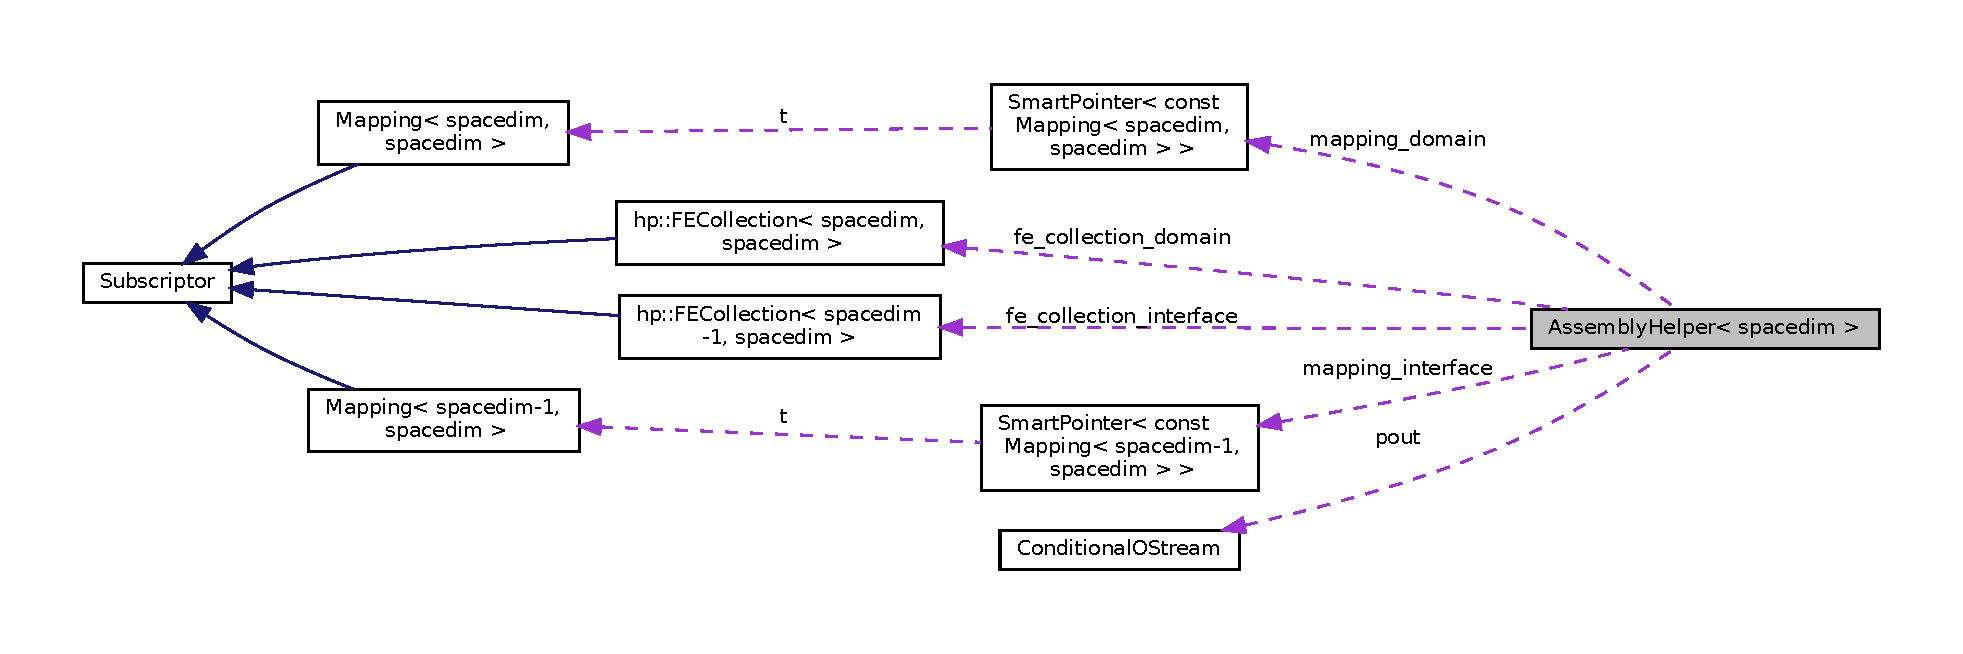
\includegraphics[width=350pt]{class_assembly_helper__coll__graph}
\end{center}
\end{figure}
\doxysubsection*{Public Member Functions}
\begin{DoxyCompactItemize}
\item 
\mbox{\hyperlink{class_assembly_helper_ae164448dcc5e9e8d2849c354212d6df5}{Assembly\+Helper}} (const \mbox{\hyperlink{class_total_potential}{Total\+Potential}}$<$ spacedim $>$ \&\mbox{\hyperlink{class_assembly_helper_a748eed9d73b7437a4bf2dcd73108790b}{total\+\_\+potential}}, \mbox{\hyperlink{class_triangulation_system}{Triangulation\+System}}$<$ spacedim $>$ \&\mbox{\hyperlink{class_assembly_helper_add08a8a7bb9c9325fcc7d92bfce525d4}{tria\+\_\+system}}, const \textbf{ Mapping}$<$ spacedim, spacedim $>$ \&\mbox{\hyperlink{class_assembly_helper_a3fbb49461000dea8f64266f830709fad}{mapping\+\_\+domain}}, const \textbf{ Mapping}$<$ spacedim-\/1, spacedim $>$ \&\mbox{\hyperlink{class_assembly_helper_a055fde6217c18e62cd80188d0130c201}{mapping\+\_\+interface}}, const std\+::set$<$ const \mbox{\hyperlink{class_independent_field}{Independent\+Field}}$<$ 0, spacedim $>$ $\ast$ $>$ \&independent\+\_\+scalars=std\+::set$<$ const \mbox{\hyperlink{class_independent_field}{Independent\+Field}}$<$ 0, spacedim $>$ $\ast$ $>$())
\item 
\mbox{\hyperlink{class_assembly_helper_ac82eca7b04aedf772028c6ff77245e9b}{$\sim$\+Assembly\+Helper}} ()
\end{DoxyCompactItemize}
\begin{Indent}\textbf{ Methods for assembly of the finite element system}\par
\begin{DoxyCompactItemize}
\item 
{\footnotesize template$<$class Vector\+Type $>$ }\\void \mbox{\hyperlink{class_assembly_helper_a4043c993c8902ad5d3045a13ed42e6f8}{get\+\_\+initial\+\_\+fields\+\_\+vector}} (\textbf{ Vector\+Type} \&initial\+\_\+fields, const Affine\+Constraints$<$ double $>$ $\ast$constraints=nullptr) const
\item 
void \mbox{\hyperlink{class_assembly_helper_a40e7eb10c5dbd5358597f38291b90d85}{make\+\_\+dirichlet\+\_\+constraints}} (Affine\+Constraints$<$ double $>$ \&constraint\+\_\+matrix, const std\+::vector$<$ const \mbox{\hyperlink{class_dirichlet_constraint}{Dirichlet\+Constraint}}$<$ spacedim $>$ $\ast$ $>$ \&dirichlet\+\_\+constraints, const Affine\+Constraints$<$ double $>$ \&constraints\+\_\+ignore=Affine\+Constraints$<$ double $>$()) const
\item 
void \mbox{\hyperlink{class_assembly_helper_a5b2d6681755428d4abfe718e54e3c322}{make\+\_\+dirichlet\+\_\+constraints}} (Affine\+Constraints$<$ double $>$ \&constraint\+\_\+matrix, const std\+::vector$<$ const \mbox{\hyperlink{class_dirichlet_constraint}{Dirichlet\+Constraint}}$<$ spacedim $>$ $\ast$ $>$ \&dirichlet\+\_\+constraints, const std\+::vector$<$ const \mbox{\hyperlink{class_point_constraint}{Point\+Constraint}}$<$ spacedim, spacedim $>$ $\ast$ $>$ \&point\+\_\+constraints\+\_\+omega, const std\+::vector$<$ const \mbox{\hyperlink{class_point_constraint}{Point\+Constraint}}$<$ spacedim-\/1, spacedim $>$ $\ast$ $>$ \&point\+\_\+constraints\+\_\+sigma, const std\+::vector$<$ const \mbox{\hyperlink{class_point_constraint}{Point\+Constraint}}$<$ 0, spacedim $>$ $\ast$ $>$ \&point\+\_\+constraints\+\_\+C, const Affine\+Constraints$<$ double $>$ \&constraints\+\_\+ignore=Affine\+Constraints$<$ double $>$()) const
\item 
{\footnotesize template$<$class Sparsity\+Pattern\+Type $>$ }\\void \mbox{\hyperlink{class_assembly_helper_a60a2aa2aa08149682feca02e458232d4}{generate\+\_\+sparsity\+\_\+pattern\+\_\+by\+\_\+simulation}} (Sparsity\+Pattern\+Type \&dsp\+\_\+K, const Affine\+Constraints$<$ double $>$ \&constraints) const
\item 
{\footnotesize template$<$class Solution\+Vector\+Type , class R\+H\+S\+Vector\+Type , class Matrix\+Type $>$ }\\bool \mbox{\hyperlink{class_assembly_helper_ae02fef45662d1703b0f29d7d9cead7c1}{assemble\+\_\+system}} (const Solution\+Vector\+Type \&solution, const std\+::vector$<$ const Solution\+Vector\+Type $\ast$ $>$ solution\+\_\+ref\+\_\+sets, const Affine\+Constraints$<$ double $>$ \&constraints, double \&potential\+\_\+value, R\+H\+S\+Vector\+Type \&f, Matrix\+Type \&K, const std\+::tuple$<$ bool, bool, bool $>$ requested\+\_\+quantities=std\+::make\+\_\+tuple(true, true, true)) const
\item 
{\footnotesize template$<$class Vector\+Type $>$ }\\bool \mbox{\hyperlink{class_assembly_helper_acf6ef2dced66e223684e5df97182f428}{get\+\_\+nonprimitive\+\_\+scalar\+\_\+functional\+\_\+values}} (const \textbf{ Vector\+Type} \&solution, const std\+::vector$<$ const \textbf{ Vector\+Type} $\ast$ $>$ solution\+\_\+ref\+\_\+sets, std\+::map$<$ const \mbox{\hyperlink{class_scalar_functional}{Scalar\+Functional}}$<$ spacedim, spacedim $>$ $\ast$, double $>$ \&nonprimitive\+\_\+scalar\+\_\+functional\+\_\+values\+\_\+domain, std\+::map$<$ const \mbox{\hyperlink{class_scalar_functional}{Scalar\+Functional}}$<$ spacedim-\/1, spacedim $>$ $\ast$, double $>$ \&nonprimitive\+\_\+scalar\+\_\+functional\+\_\+values\+\_\+interface) const
\item 
{\footnotesize template$<$class Vector\+Type $>$ }\\double \mbox{\hyperlink{class_assembly_helper_a310594206df2622027fdc48e84600bf7}{get\+\_\+maximum\+\_\+step\+\_\+length}} (const \textbf{ Vector\+Type} \&solution, const std\+::vector$<$ const \textbf{ Vector\+Type} $\ast$ $>$ solution\+\_\+ref\+\_\+sets, const \textbf{ Vector\+Type} \&delta\+\_\+solution) const
\item 
{\footnotesize template$<$class Vector\+Type $>$ }\\void \mbox{\hyperlink{class_assembly_helper_ac54f45f37a38426db1b5f85eccc7b3e9}{compare\+\_\+derivatives\+\_\+with\+\_\+numerical\+\_\+derivatives}} (const \textbf{ Vector\+Type} \&solution, const std\+::vector$<$ const \textbf{ Vector\+Type} $\ast$ $>$ solution\+\_\+ref\+\_\+sets, const std\+::string detailed\+\_\+printout\+\_\+file=\char`\"{}\char`\"{}, const double \textbf{ epsilon}=1\textbf{ e}-\/8) const
\end{DoxyCompactItemize}
\end{Indent}
\begin{Indent}\textbf{ Methods for writing output}\par
\begin{DoxyCompactItemize}
\item 
{\footnotesize template$<$class Vector\+Type $>$ }\\std\+::pair$<$ const std\+::string, const std\+::string $>$ \mbox{\hyperlink{class_assembly_helper_a6120d66724f518dcfcdc30a89df01c23}{write\+\_\+output\+\_\+independent\+\_\+fields}} (const \textbf{ Vector\+Type} \&solution, const std\+::string file\+\_\+name\+\_\+domain, const std\+::string file\+\_\+name\+\_\+interface, const unsigned int file\+\_\+index=0, const std\+::vector$<$ dealii\+::\+Smart\+Pointer$<$ const dealii\+::\+Data\+Postprocessor$<$ spacedim $>$$>$$>$ \&dp\+\_\+domain=std\+::vector$<$ dealii\+::\+Smart\+Pointer$<$ const dealii\+::\+Data\+Postprocessor$<$ spacedim $>$$>$$>$(), const std\+::vector$<$ dealii\+::\+Smart\+Pointer$<$ const dealii\+::\+Data\+Postprocessor$<$ spacedim $>$$>$$>$ \&dp\+\_\+interface=std\+::vector$<$ dealii\+::\+Smart\+Pointer$<$ const dealii\+::\+Data\+Postprocessor$<$ spacedim $>$$>$$>$(), const unsigned int n\+\_\+subdivisions=1) const
\item 
void \mbox{\hyperlink{class_assembly_helper_a6a6f8ff7c1a8910d84beb7761b5c821b}{print\+\_\+assembly\+\_\+helper\+\_\+definition}} (const bool detailed\+\_\+printout\+\_\+shapefuns=true) const
\end{DoxyCompactItemize}
\end{Indent}
\begin{Indent}\textbf{ Methods for comparing solutions}\par
{\em These methods are essentially intended for studies of the convergence behavior. Two types of methods are offered. The first allows comparison with a different numerical solution obtained on a differently refined mesh; and the second allows comparison with an analytical solution. }\begin{DoxyCompactItemize}
\item 
{\footnotesize template$<$class Vector\+Type $>$ }\\std\+::pair$<$ const double, const double $>$ \mbox{\hyperlink{class_assembly_helper_a94bb821b6258eab0bb3a9046b6d9158a}{compute\+\_\+distance\+\_\+to\+\_\+other\+\_\+solution}} (const \textbf{ Vector\+Type} \&solution, const \textbf{ Vector\+Type} \&other\+\_\+solution, const \mbox{\hyperlink{class_assembly_helper}{Assembly\+Helper}}$<$ spacedim $>$ \&other\+\_\+assembly\+\_\+helper, const \textbf{ Quadrature}$<$ spacedim $>$ quadrature\+\_\+domain, const \textbf{ Quadrature}$<$ spacedim-\/1 $>$ quadrature\+\_\+interface, const \textbf{ Vector\+Tools\+::\+Norm\+Type} norm\+\_\+type=Vector\+Tools\+::\+Norm\+Type\+::\+L2\+\_\+norm, const \textbf{ Component\+Mask} component\+\_\+mask\+\_\+domain=\textbf{ Component\+Mask}(), const \textbf{ Component\+Mask} component\+\_\+mask\+\_\+interface=\textbf{ Component\+Mask}(), const double exponent=2.\+0, const \textbf{ Vector}$<$ double $>$ scaling\+\_\+domain=\textbf{ dealii\+::\+Vector}$<$ double $>$(), const \textbf{ Vector}$<$ double $>$ scaling\+\_\+interface=\textbf{ dealii\+::\+Vector}$<$ double $>$()) const
\item 
{\footnotesize template$<$class Vector\+Type $>$ }\\std\+::pair$<$ const double, const double $>$ \mbox{\hyperlink{class_assembly_helper_a0e96514d9d023949eb07d95b5a2214c4}{compute\+\_\+distance\+\_\+to\+\_\+exact\+\_\+solution}} (const \textbf{ Vector\+Type} \&solution, const \textbf{ Function}$<$ spacedim $>$ \&exact\+\_\+solution\+\_\+domain, const \textbf{ Function}$<$ spacedim $>$ \&exact\+\_\+solution\+\_\+interface, const \textbf{ Quadrature}$<$ spacedim $>$ quadrature\+\_\+domain, const \textbf{ Quadrature}$<$ spacedim-\/1 $>$ quadrature\+\_\+interface, const \textbf{ Vector\+Tools\+::\+Norm\+Type} norm\+\_\+type=Vector\+Tools\+::\+Norm\+Type\+::\+L2\+\_\+norm, const \textbf{ Component\+Mask} component\+\_\+mask\+\_\+domain=\textbf{ Component\+Mask}(), const \textbf{ Component\+Mask} component\+\_\+mask\+\_\+interface=\textbf{ Component\+Mask}(), const double exponent=2.\+0) const
\end{DoxyCompactItemize}
\end{Indent}
\begin{Indent}\textbf{ Methods for querying information about the Assembly\+Helper object.}\par
\begin{DoxyCompactItemize}
\item 
const \mbox{\hyperlink{class_triangulation_system}{Triangulation\+System}}$<$ spacedim $>$ \& \mbox{\hyperlink{class_assembly_helper_a42cc83a6b33fe48b04fa8f4c9907cbb8}{get\+\_\+triangulation\+\_\+system}} () const
\item 
\mbox{\hyperlink{class_triangulation_system}{Triangulation\+System}}$<$ spacedim $>$ \& \mbox{\hyperlink{class_assembly_helper_a16f9d21a79922d4879e37916b414f7d0}{get\+\_\+triangulation\+\_\+system}} ()
\item 
const \mbox{\hyperlink{class_do_f_handler_system}{Do\+F\+Handler\+System}}$<$ spacedim $>$ \& \mbox{\hyperlink{class_assembly_helper_a095623df46217c89ee8e786f6e8a3034}{get\+\_\+dof\+\_\+handler\+\_\+system}} () const
\item 
\mbox{\hyperlink{class_do_f_handler_system}{Do\+F\+Handler\+System}}$<$ spacedim $>$ \& \mbox{\hyperlink{class_assembly_helper_a04523eef6062ced8c88d4c093b65df3d}{get\+\_\+dof\+\_\+handler\+\_\+system}} ()
\item 
std\+::map$<$ const \mbox{\hyperlink{class_independent_field}{Independent\+Field}}$<$ spacedim, spacedim $>$ $\ast$, const unsigned int $>$ \mbox{\hyperlink{class_assembly_helper_a39d6fed5b90cee2e2e972e294ececffb}{get\+\_\+u\+\_\+omega\+\_\+global\+\_\+component\+\_\+indices}} () const
\item 
std\+::map$<$ const \mbox{\hyperlink{class_independent_field}{Independent\+Field}}$<$ spacedim-\/1, spacedim $>$ $\ast$, const unsigned int $>$ \mbox{\hyperlink{class_assembly_helper_afe7df3baf877b83b7c98b7f389fa2926}{get\+\_\+u\+\_\+sigma\+\_\+global\+\_\+component\+\_\+indices}} () const
\item 
unsigned int \mbox{\hyperlink{class_assembly_helper_af65861aae14b724a631feaf56c82ae9a}{get\+\_\+u\+\_\+omega\+\_\+global\+\_\+component\+\_\+index}} (const \mbox{\hyperlink{class_independent_field}{Independent\+Field}}$<$ spacedim, spacedim $>$ \&\mbox{\hyperlink{class_assembly_helper_a1952a054a839a7a683ca108013e7d976}{u\+\_\+omega}}) const
\item 
unsigned int \mbox{\hyperlink{class_assembly_helper_a4ad9cb7482bfc3ce527ad7639a8d5843}{get\+\_\+u\+\_\+sigma\+\_\+global\+\_\+component\+\_\+index}} (const \mbox{\hyperlink{class_independent_field}{Independent\+Field}}$<$ spacedim-\/1, spacedim $>$ \&\mbox{\hyperlink{class_assembly_helper_a696fe649b3503561235aa1ccbf2ddeef}{u\+\_\+sigma}}) const
\item 
unsigned int \mbox{\hyperlink{class_assembly_helper_ae821c8ae9c8fa6f8e85d20ecd5ad7e39}{system\+\_\+size}} () const
\item 
unsigned int \mbox{\hyperlink{class_assembly_helper_a781fcbb9a157621c8db25d8ef46aca13}{get\+\_\+n\+\_\+stretched\+\_\+rows}} () const
\item 
unsigned int \mbox{\hyperlink{class_assembly_helper_a9b9603ede43f9abae845caf60e52d4a1}{get\+\_\+n\+\_\+C}} () const
\item 
unsigned int \mbox{\hyperlink{class_assembly_helper_a3b6e5ff3a45411c2b8b42777fa94ec40}{get\+\_\+global\+\_\+dof\+\_\+index\+\_\+C}} (const \mbox{\hyperlink{class_independent_field}{Independent\+Field}}$<$ 0, spacedim $>$ $\ast$independent\+\_\+scalar) const
\item 
const \textbf{ Index\+Set} \mbox{\hyperlink{class_assembly_helper_a30584e0ed1b2564e9b66ce9cecae40c7}{get\+\_\+locally\+\_\+relevant\+\_\+indices}} () const
\item 
const \textbf{ Index\+Set} \mbox{\hyperlink{class_assembly_helper_a8ecc73fbc0e71716805c97498a83833a}{get\+\_\+locally\+\_\+owned\+\_\+indices}} () const
\item 
const std\+::vector$<$ \textbf{ Index\+Set} $>$ \mbox{\hyperlink{class_assembly_helper_a5f47fad7f7f2a83a7f54cd38825c703a}{get\+\_\+locally\+\_\+relevant\+\_\+indices\+\_\+blocks}} () const
\item 
const std\+::vector$<$ \textbf{ Index\+Set} $>$ \mbox{\hyperlink{class_assembly_helper_af1a81fd16e7692501189d9c0bd96bc2d}{get\+\_\+locally\+\_\+owned\+\_\+indices\+\_\+blocks}} () const
\item 
unsigned int \mbox{\hyperlink{class_assembly_helper_a9950dbca7be157c964bd7403fccfde8a}{get\+\_\+dof\+\_\+index\+\_\+at\+\_\+point\+\_\+omega}} (const \mbox{\hyperlink{class_independent_field}{Independent\+Field}}$<$ spacedim, spacedim $>$ $\ast$\mbox{\hyperlink{class_assembly_helper_a1952a054a839a7a683ca108013e7d976}{u\+\_\+omega}}, const unsigned int component, const \textbf{ Point}$<$ spacedim $>$ p) const
\item 
unsigned int \mbox{\hyperlink{class_assembly_helper_a1272cbcddc6b23108d3e090c2e704339}{get\+\_\+dof\+\_\+index\+\_\+at\+\_\+point\+\_\+sigma}} (const \mbox{\hyperlink{class_independent_field}{Independent\+Field}}$<$ spacedim-\/1, spacedim $>$ $\ast$\mbox{\hyperlink{class_assembly_helper_a696fe649b3503561235aa1ccbf2ddeef}{u\+\_\+sigma}}, const unsigned int component, const \textbf{ Point}$<$ spacedim $>$ p) const
\item 
void \mbox{\hyperlink{class_assembly_helper_ab0dabb84cc4a0497dbeb73a9eec3071d}{print\+\_\+dof\+\_\+information}} (const unsigned int dof\+\_\+index) const
\end{DoxyCompactItemize}
\end{Indent}
\doxysubsection*{Private Member Functions}
\begin{Indent}\textbf{ Member functions used during construction of an Assembly\+Helper object}\par
{\em These functions are essentially introduced to clean up tthe constructor of the class a bit. They are only used during construction of an \mbox{\hyperlink{class_assembly_helper}{Assembly\+Helper}} object. }\begin{DoxyCompactItemize}
\item 
void \mbox{\hyperlink{class_assembly_helper_aad21ced11a2d90c804827854c18f7f89}{convert\+\_\+dependent\+\_\+fields\+\_\+to\+\_\+shapefunctions}} ()
\item 
void \mbox{\hyperlink{class_assembly_helper_a1c187fbb8171d6a1ff2ff6344cb454ed}{initialize\+\_\+hidden\+\_\+variables}} () const
\end{DoxyCompactItemize}
\end{Indent}
\begin{Indent}\textbf{ Member functions related to assembly of the finite element system}\par
{\em These functions are all needed during assembly of the finite element system. }\begin{DoxyCompactItemize}
\item 
void \mbox{\hyperlink{class_assembly_helper_a953859cc4cd745a1b51fdec5418be682}{distribute\+\_\+dofs}} ()
\item 
void \mbox{\hyperlink{class_assembly_helper_a2c394d614e7ffe8b81ba1a8623db611d}{initialize\+\_\+fe\+\_\+values\+\_\+domain}} (const typename \textbf{ hp\+::\+Do\+F\+Handler}$<$ spacedim, spacedim $>$\+::\textbf{ active\+\_\+cell\+\_\+iterator} \&cell, const unsigned int internal\+\_\+index, const bool nonprimitive=false) const
\item 
void \mbox{\hyperlink{class_assembly_helper_a223bbebe8a1f0aa09a53ee19257b927e}{initialize\+\_\+fe\+\_\+values\+\_\+interface}} (const \mbox{\hyperlink{class_interface_cell_domain_cells_do_f}{Interface\+Cell\+Domain\+Cells\+DoF}}$<$ spacedim $>$ \&interface\+\_\+cell\+\_\+domain\+\_\+cells, const unsigned int internal\+\_\+index, const bool nonprimitive=false) const
\item 
void \mbox{\hyperlink{class_assembly_helper_a5e29275d9ec1c479375707fbc670bc8c}{compute\+\_\+e\+\_\+omega}} (const unsigned int internal\+\_\+index, const unsigned int scalar\+\_\+functional\+\_\+index, const unsigned int q\+\_\+point, const \textbf{ Vector}$<$ double $>$ \&solution\+\_\+u\+\_\+omega, const \textbf{ Vector}$<$ double $>$ \&solution\+\_\+C, \textbf{ Vector}$<$ double $>$ \&e\+\_\+omega, \textbf{ Full\+Matrix}$<$ double $>$ \&de\+\_\+omega\+\_\+dsol\+\_\+T, const bool compute\+\_\+derivative=true, const bool ignore\+\_\+constants=false) const
\item 
void \mbox{\hyperlink{class_assembly_helper_a1906ba80994e8bb136ccf466fd7611d5}{compute\+\_\+e\+\_\+sigma}} (const unsigned int internal\+\_\+index, const unsigned int scalar\+\_\+functional\+\_\+index, const unsigned int q\+\_\+point, const \textbf{ Vector}$<$ double $>$ \&solution\+\_\+u\+\_\+sigma, const \textbf{ Vector}$<$ double $>$ \&solution\+\_\+u\+\_\+omega\+\_\+minus, const \textbf{ Vector}$<$ double $>$ \&solution\+\_\+u\+\_\+omega\+\_\+plus, const \textbf{ Vector}$<$ double $>$ \&solution\+\_\+C, const std\+::vector$<$ unsigned int $>$ \&dof\+\_\+indices\+\_\+interface\+\_\+dof\+\_\+indices\+\_\+combined, const std\+::vector$<$ unsigned int $>$ \&dof\+\_\+indices\+\_\+minus\+\_\+dof\+\_\+indices\+\_\+combined, const std\+::vector$<$ unsigned int $>$ \&dof\+\_\+indices\+\_\+plus\+\_\+dof\+\_\+indices\+\_\+combined, const std\+::vector$<$ unsigned int $>$ \&dof\+\_\+indices\+\_\+\+C\+\_\+dof\+\_\+indices\+\_\+combined, const std\+::vector$<$ unsigned int $>$ \&dof\+\_\+indices\+\_\+global\+\_\+combined, \textbf{ Vector}$<$ double $>$ \&e\+\_\+sigma, \textbf{ Full\+Matrix}$<$ double $>$ \&de\+\_\+sigma\+\_\+dsol\+\_\+T, const bool compute\+\_\+derivative=true, const bool ignore\+\_\+constants=false) const
\item 
{\footnotesize template$<$class Vector\+Type $>$ }\\bool \mbox{\hyperlink{class_assembly_helper_abe88d8ccfd69bbfcfc56551c5c7d67e9}{get\+\_\+nonprimitive\+\_\+scalar\+\_\+functional\+\_\+values}} (const \textbf{ Vector\+Type} \&solution, const std\+::vector$<$ const \textbf{ Vector\+Type} $\ast$ $>$ solution\+\_\+ref\+\_\+sets, \textbf{ Vector}$<$ double $>$ \&nonprimitive\+\_\+scalar\+\_\+functional\+\_\+values) const
\item 
std\+::pair$<$ const int, const int $>$ \mbox{\hyperlink{class_assembly_helper_a2778924ff66c8ad8695f0cd3da5ced9f}{get\+\_\+scalar\+\_\+functional\+\_\+indices}} (const \mbox{\hyperlink{class_scalar_functional}{Scalar\+Functional}}$<$ spacedim, spacedim $>$ $\ast$scalar\+\_\+functional) const
\item 
std\+::pair$<$ const int, const int $>$ \mbox{\hyperlink{class_assembly_helper_a3e3f6a06344be172d9419b26bb085073}{get\+\_\+scalar\+\_\+functional\+\_\+indices}} (const \mbox{\hyperlink{class_scalar_functional}{Scalar\+Functional}}$<$ spacedim-\/1, spacedim $>$ $\ast$scalar\+\_\+functional) const
\item 
void \mbox{\hyperlink{class_assembly_helper_ae339631f070dbe766d84697cd9229134}{get\+\_\+dof\+\_\+indices\+\_\+C}} (std\+::vector$<$ unsigned int $>$ \&global\+\_\+dof\+\_\+indices\+\_\+C) const
\item 
void \mbox{\hyperlink{class_assembly_helper_a8a6d7a10dfa2b88ef6f2a974124b0ad5}{make\+\_\+dirichlet\+\_\+constraints\+\_\+recursion}} (const typename \mbox{\hyperlink{class_triangulation_system}{Triangulation\+System}}$<$ spacedim $>$\+::Domain\+Cell \&domain\+\_\+cell, const unsigned int face, const std\+::vector$<$ unsigned int $>$ \&shapefuns, const \mbox{\hyperlink{class_dirichlet_constraint}{Dirichlet\+Constraint}}$<$ spacedim $>$ \&constraint, Affine\+Constraints$<$ double $>$ \&constraint\+\_\+matrix, const Affine\+Constraints$<$ double $>$ \&constraints\+\_\+ignore) const
\end{DoxyCompactItemize}
\end{Indent}
\doxysubsection*{Private Attributes}
\begin{Indent}\textbf{ Problem definition}\par
{\em These members define the problem to be solved. }\begin{DoxyCompactItemize}
\item 
const \mbox{\hyperlink{class_total_potential}{Total\+Potential}}$<$ spacedim $>$ \mbox{\hyperlink{class_assembly_helper_a748eed9d73b7437a4bf2dcd73108790b}{total\+\_\+potential}}
\item 
\mbox{\hyperlink{class_triangulation_system}{Triangulation\+System}}$<$ spacedim $>$ \& \mbox{\hyperlink{class_assembly_helper_add08a8a7bb9c9325fcc7d92bfce525d4}{tria\+\_\+system}}
\item 
const \textbf{ Smart\+Pointer}$<$ const \textbf{ Mapping}$<$ spacedim, spacedim $>$ $>$ \mbox{\hyperlink{class_assembly_helper_a3fbb49461000dea8f64266f830709fad}{mapping\+\_\+domain}}
\item 
const \textbf{ Smart\+Pointer}$<$ const \textbf{ Mapping}$<$ spacedim-\/1, spacedim $>$ $>$ \mbox{\hyperlink{class_assembly_helper_a055fde6217c18e62cd80188d0130c201}{mapping\+\_\+interface}}
\end{DoxyCompactItemize}
\end{Indent}
\begin{Indent}\textbf{ Domain and interface portion indexing}\par
{\em These members define consecutive indices for domain and interface portions for internal use. }\begin{DoxyCompactItemize}
\item 
std\+::map$<$ \textbf{ types\+::material\+\_\+id}, const unsigned int $>$ \mbox{\hyperlink{class_assembly_helper_a10b3acf64bccc169ee14dc2505ce4b46}{material\+\_\+id\+\_\+to\+\_\+internal\+\_\+index\+\_\+domain}}
\item 
std\+::map$<$ std\+::tuple$<$ const \textbf{ types\+::material\+\_\+id}, const \textbf{ types\+::material\+\_\+id}, const \textbf{ types\+::material\+\_\+id} $>$, const unsigned int $>$ \mbox{\hyperlink{class_assembly_helper_a43b82de0ede96d03b9f7fd8740d81668}{material\+\_\+ids\+\_\+to\+\_\+internal\+\_\+index\+\_\+interface}}
\end{DoxyCompactItemize}
\end{Indent}
\begin{Indent}\textbf{ Finite elements and dof handling}\par
{\em These members comprise the finite elements to be used on the respective domain and interface portions as well as the \mbox{\hyperlink{class_do_f_handler_system}{Do\+F\+Handler\+System}} (which contains all dof information). }\begin{DoxyCompactItemize}
\item 
\textbf{ hp\+::\+F\+E\+Collection}$<$ spacedim, spacedim $>$ \mbox{\hyperlink{class_assembly_helper_af3803b0aad9853e6bf018c70be41e791}{fe\+\_\+collection\+\_\+domain}}
\item 
\textbf{ hp\+::\+F\+E\+Collection}$<$ spacedim-\/1, spacedim $>$ \mbox{\hyperlink{class_assembly_helper_a8b4d224a9ecd2e926a8860829874d2a1}{fe\+\_\+collection\+\_\+interface}}
\item 
std\+::map$<$ \textbf{ types\+::material\+\_\+id}, unsigned int $>$ \mbox{\hyperlink{class_assembly_helper_a3045f80801fc31920efd161a268aae8e}{material\+\_\+id\+\_\+to\+\_\+fe\+\_\+system\+\_\+id\+\_\+domain}}
\item 
std\+::map$<$ \textbf{ types\+::material\+\_\+id}, unsigned int $>$ \mbox{\hyperlink{class_assembly_helper_a5fea54137e3c1c5a514e39c9b2ad7926}{material\+\_\+id\+\_\+to\+\_\+fe\+\_\+system\+\_\+id\+\_\+interface}}
\item 
\mbox{\hyperlink{class_do_f_handler_system}{Do\+F\+Handler\+System}}$<$ spacedim $>$ \mbox{\hyperlink{class_assembly_helper_a885e660c749e91a35e3279643ebcd87f}{dof\+\_\+handler\+\_\+system}}
\end{DoxyCompactItemize}
\end{Indent}
\begin{Indent}\textbf{ Members re-\/organizing Assembly\+Helper\+::total\+\_\+potential}\par
{\em These members re-\/organize the information provided by \mbox{\hyperlink{class_assembly_helper_a748eed9d73b7437a4bf2dcd73108790b}{Assembly\+Helper\+::total\+\_\+potential}} in a way suitable for efficient assembly of the finite element system. }\begin{DoxyCompactItemize}
\item 
std\+::vector$<$ \textbf{ Smart\+Pointer}$<$ const \mbox{\hyperlink{class_independent_field}{Independent\+Field}}$<$ spacedim, spacedim $>$ $>$ $>$ \mbox{\hyperlink{class_assembly_helper_a1952a054a839a7a683ca108013e7d976}{u\+\_\+omega}}
\item 
std\+::vector$<$ \textbf{ Smart\+Pointer}$<$ const \mbox{\hyperlink{class_independent_field}{Independent\+Field}}$<$ spacedim-\/1, spacedim $>$ $>$ $>$ \mbox{\hyperlink{class_assembly_helper_a696fe649b3503561235aa1ccbf2ddeef}{u\+\_\+sigma}}
\item 
std\+::vector$<$ \textbf{ Smart\+Pointer}$<$ const \mbox{\hyperlink{class_independent_field}{Independent\+Field}}$<$ 0, spacedim $>$ $>$ $>$ \mbox{\hyperlink{class_assembly_helper_aa5234a46be82cfe7d92678169d38f326}{C}}
\item 
std\+::map$<$ \textbf{ Smart\+Pointer}$<$ const \mbox{\hyperlink{class_independent_field}{Independent\+Field}}$<$ spacedim, spacedim $>$ $>$, const unsigned int $>$ \mbox{\hyperlink{class_assembly_helper_a6dae4b6ae7934eaec1ad7baff258ce6e}{global\+\_\+component\+\_\+indices\+\_\+u\+\_\+omega}}
\item 
std\+::map$<$ \textbf{ Smart\+Pointer}$<$ const \mbox{\hyperlink{class_independent_field}{Independent\+Field}}$<$ spacedim-\/1, spacedim $>$ $>$, const unsigned int $>$ \mbox{\hyperlink{class_assembly_helper_a992a53a1fcac8a393ca53fb8d504bdfe}{global\+\_\+component\+\_\+indices\+\_\+u\+\_\+sigma}}
\item 
std\+::map$<$ \textbf{ Smart\+Pointer}$<$ const \mbox{\hyperlink{class_independent_field}{Independent\+Field}}$<$ 0, spacedim $>$ $>$, const unsigned int $>$ \mbox{\hyperlink{class_assembly_helper_a9a8f0e8ea8c67ce9429c16a2017cafdc}{global\+\_\+indices\+\_\+C}}
\item 
std\+::vector$<$ std\+::vector$<$ \textbf{ Smart\+Pointer}$<$ const \mbox{\hyperlink{class_scalar_functional}{Scalar\+Functional}}$<$ spacedim, spacedim $>$ $>$ $>$ $>$ \mbox{\hyperlink{class_assembly_helper_aa6fa619e4c2582e95950e878cd06628e}{scalar\+\_\+functionals\+\_\+domain}}
\item 
std\+::vector$<$ std\+::vector$<$ \textbf{ Smart\+Pointer}$<$ const \mbox{\hyperlink{class_scalar_functional}{Scalar\+Functional}}$<$ spacedim-\/1, spacedim $>$ $>$ $>$ $>$ \mbox{\hyperlink{class_assembly_helper_a29aa77e0e8e6b35c94966ea88840e462}{scalar\+\_\+functionals\+\_\+interface}}
\item 
std\+::vector$<$ std\+::vector$<$ unsigned int $>$ $>$ \mbox{\hyperlink{class_assembly_helper_a5fe78a019aec03cbeeb336d1d2874729}{scalar\+\_\+functionals\+\_\+domain\+\_\+nonprimitive}}
\item 
std\+::vector$<$ std\+::vector$<$ unsigned int $>$ $>$ \mbox{\hyperlink{class_assembly_helper_a833383aa6d157157545204143897ed9e}{scalar\+\_\+functionals\+\_\+interface\+\_\+nonprimitive}}
\item 
std\+::map$<$ \textbf{ Smart\+Pointer}$<$ const \mbox{\hyperlink{class_scalar_functional}{Scalar\+Functional}}$<$ spacedim, spacedim $>$ $>$, const unsigned int $>$ \mbox{\hyperlink{class_assembly_helper_acf05fab2ddf57769a103d82a4f2d1cd3}{scalar\+\_\+functionals\+\_\+domain\+\_\+nonprimitive\+\_\+indices}}
\item 
std\+::map$<$ \textbf{ Smart\+Pointer}$<$ const \mbox{\hyperlink{class_scalar_functional}{Scalar\+Functional}}$<$ spacedim-\/1, spacedim $>$ $>$, const unsigned int $>$ \mbox{\hyperlink{class_assembly_helper_a0d15b3ab0c7bec9fc4f40e532f8776f4}{scalar\+\_\+functionals\+\_\+interface\+\_\+nonprimitive\+\_\+indices}}
\item 
std\+::map$<$ \textbf{ Smart\+Pointer}$<$ const \mbox{\hyperlink{class_scalar_functional}{Scalar\+Functional}}$<$ spacedim, spacedim $>$ $>$, const unsigned int $>$ \mbox{\hyperlink{class_assembly_helper_a4f08790a2235e48ce19f5d8d965a7874}{scalar\+\_\+functionals\+\_\+domain\+\_\+primitive\+\_\+indices}}
\item 
std\+::map$<$ \textbf{ Smart\+Pointer}$<$ const \mbox{\hyperlink{class_scalar_functional}{Scalar\+Functional}}$<$ spacedim-\/1, spacedim $>$ $>$, const unsigned int $>$ \mbox{\hyperlink{class_assembly_helper_ad99c75f32cf3f18aa1d4067ad8b56ae8}{scalar\+\_\+functionals\+\_\+interface\+\_\+primitive\+\_\+indices}}
\item 
std\+::map$<$ \textbf{ Smart\+Pointer}$<$ const \mbox{\hyperlink{class_scalar_functional}{Scalar\+Functional}}$<$ spacedim, spacedim $>$ $>$, std\+::vector$<$ std\+::pair$<$ const unsigned int, const unsigned int $>$ $>$ $>$ \mbox{\hyperlink{class_assembly_helper_aceaf7ba62dfe0fa06ecb15ee8c14da34}{contributions\+\_\+scalar\+\_\+functionals\+\_\+domain\+\_\+total\+\_\+potential}}
\item 
std\+::map$<$ \textbf{ Smart\+Pointer}$<$ const \mbox{\hyperlink{class_scalar_functional}{Scalar\+Functional}}$<$ spacedim-\/1, spacedim $>$ $>$, std\+::vector$<$ std\+::pair$<$ const unsigned int, const unsigned int $>$ $>$ $>$ \mbox{\hyperlink{class_assembly_helper_a9e76874224ab4946218fdce9bdba0e03}{contributions\+\_\+scalar\+\_\+functionals\+\_\+interface\+\_\+total\+\_\+potential}}
\item 
unsigned int \mbox{\hyperlink{class_assembly_helper_af7bcfc1db651535a7aefc6071a81e124}{n\+\_\+scalar\+\_\+functionals\+\_\+nonprimitive}}
\item 
unsigned int \mbox{\hyperlink{class_assembly_helper_af5e03e8e47a85dbc96444ef61525c454}{n\+\_\+scalar\+\_\+functionals\+\_\+primitive}}
\end{DoxyCompactItemize}
\end{Indent}
\begin{Indent}\textbf{ Members providing information about shape function indexing, etc.}\par
{\em These data structures are organized in a way that shape function related information needed again and again for the functionalities provided by \mbox{\hyperlink{class_assembly_helper}{Assembly\+Helper}} (in particular assembly of the finite element system) can be retrieved efficiently. }\begin{DoxyCompactItemize}
\item 
std\+::vector$<$ std\+::vector$<$ std\+::vector$<$ unsigned int $>$ $>$ $>$ \mbox{\hyperlink{class_assembly_helper_a0bdb6e2e2f9623f3f10dfa2ebe8e234c}{components\+\_\+to\+\_\+shapefuns\+\_\+domain}}
\item 
std\+::vector$<$ std\+::vector$<$ std\+::vector$<$ unsigned int $>$ $>$ $>$ \mbox{\hyperlink{class_assembly_helper_abcad51e64347fc3141d2840a2835b46c}{components\+\_\+to\+\_\+shapefuns\+\_\+interface}}
\item 
std\+::vector$<$ std\+::vector$<$ std\+::vector$<$ std\+::vector$<$ unsigned int $>$ $>$ $>$ $>$ \mbox{\hyperlink{class_assembly_helper_ae92560183f1d2060265f0744a84f0349}{components\+\_\+to\+\_\+shapefuns\+\_\+domain\+\_\+facewise}}
\item 
std\+::vector$<$ std\+::vector$<$ std\+::vector$<$ unsigned int $>$ $>$ $>$ \mbox{\hyperlink{class_assembly_helper_a1a26b40224e3f04e5168accc91486493}{coupled\+\_\+dof\+\_\+indices\+\_\+scalar\+\_\+functionals\+\_\+domain}}
\item 
std\+::vector$<$ std\+::vector$<$ std\+::vector$<$ unsigned int $>$ $>$ $>$ \mbox{\hyperlink{class_assembly_helper_ab346e146cf91fb7a0688076551b37355}{coupled\+\_\+dof\+\_\+indices\+\_\+scalar\+\_\+functionals\+\_\+interface}}
\item 
std\+::vector$<$ std\+::vector$<$ std\+::vector$<$ unsigned int $>$ $>$ $>$ \mbox{\hyperlink{class_assembly_helper_a12299d82365553a21fef8529c8fe8a17}{coupled\+\_\+dof\+\_\+indices\+\_\+scalar\+\_\+functionals\+\_\+interface\+\_\+minus}}
\item 
std\+::vector$<$ std\+::vector$<$ std\+::vector$<$ unsigned int $>$ $>$ $>$ \mbox{\hyperlink{class_assembly_helper_af07bb528fdd350e9b467b08dc44a03e7}{coupled\+\_\+dof\+\_\+indices\+\_\+scalar\+\_\+functionals\+\_\+interface\+\_\+plus}}
\item 
std\+::vector$<$ std\+::vector$<$ std\+::vector$<$ unsigned int $>$ $>$ $>$ \mbox{\hyperlink{class_assembly_helper_a0edd25820c92a25ae87fc240f4916804}{coupled\+\_\+\+C\+\_\+indices\+\_\+scalar\+\_\+functionals\+\_\+domain}}
\item 
std\+::vector$<$ std\+::vector$<$ std\+::vector$<$ unsigned int $>$ $>$ $>$ \mbox{\hyperlink{class_assembly_helper_a311e176038ee2b7ca0719abb384ca57b}{coupled\+\_\+\+C\+\_\+indices\+\_\+scalar\+\_\+functionals\+\_\+interface}}
\item 
std\+::vector$<$ std\+::vector$<$ std\+::vector$<$ std\+::vector$<$ std\+::tuple$<$ const double, const unsigned int, std\+::vector$<$ unsigned int $>$ $>$ $>$ $>$ $>$ $>$ \mbox{\hyperlink{class_assembly_helper_a13fef9096e5fc7b1e922ea78d7aa2c28}{a\+\_\+omega}}
\item 
std\+::vector$<$ std\+::vector$<$ std\+::vector$<$ std\+::vector$<$ std\+::tuple$<$ const double, const unsigned int, const unsigned int, std\+::vector$<$ unsigned int $>$ $>$ $>$ $>$ $>$ $>$ \mbox{\hyperlink{class_assembly_helper_a5fbb532e798c2427af5285c2df10c9f4}{b\+\_\+omega}}
\item 
std\+::vector$<$ std\+::vector$<$ std\+::vector$<$ std\+::vector$<$ std\+::tuple$<$ const double, unsigned int $>$ $>$ $>$ $>$ $>$ \mbox{\hyperlink{class_assembly_helper_a75e6f76c0b12b91c5feb230251f0137f}{c\+\_\+omega}}
\item 
std\+::vector$<$ std\+::vector$<$ std\+::vector$<$ double $>$ $>$ $>$ \mbox{\hyperlink{class_assembly_helper_ad93b109608d4425d318434e01cb6246c}{d\+\_\+omega}}
\item 
std\+::vector$<$ std\+::vector$<$ std\+::vector$<$ std\+::vector$<$ std\+::tuple$<$ const double, const unsigned int, std\+::vector$<$ unsigned int $>$ $>$ $>$ $>$ $>$ $>$ \mbox{\hyperlink{class_assembly_helper_aa266cc07e9670319481da52d633d2583}{a\+\_\+sigma}}
\item 
std\+::vector$<$ std\+::vector$<$ std\+::vector$<$ std\+::vector$<$ std\+::tuple$<$ const double, const unsigned int, const unsigned int, std\+::vector$<$ unsigned int $>$ $>$ $>$ $>$ $>$ $>$ \mbox{\hyperlink{class_assembly_helper_af58c9a1c7093edc306070913aa1b9be2}{b\+\_\+sigma}}
\item 
std\+::vector$<$ std\+::vector$<$ std\+::vector$<$ std\+::vector$<$ std\+::tuple$<$ const double, const unsigned int, std\+::vector$<$ unsigned int $>$ $>$ $>$ $>$ $>$ $>$ \mbox{\hyperlink{class_assembly_helper_a4461be378c9be0364ca23153c367d24c}{a\+\_\+minus}}
\item 
std\+::vector$<$ std\+::vector$<$ std\+::vector$<$ std\+::vector$<$ std\+::tuple$<$ const double, const unsigned int, const unsigned int, std\+::vector$<$ unsigned int $>$ $>$ $>$ $>$ $>$ $>$ \mbox{\hyperlink{class_assembly_helper_a6f51f8b4dfdae385a2e2fe2dd9e66cdb}{b\+\_\+minus}}
\item 
std\+::vector$<$ std\+::vector$<$ std\+::vector$<$ std\+::vector$<$ std\+::tuple$<$ const double, const unsigned int, std\+::vector$<$ unsigned int $>$ $>$ $>$ $>$ $>$ $>$ \mbox{\hyperlink{class_assembly_helper_a8eb513a6239d94cc0f1a6a01a037c572}{a\+\_\+plus}}
\item 
std\+::vector$<$ std\+::vector$<$ std\+::vector$<$ std\+::vector$<$ std\+::tuple$<$ const double, const unsigned int, const unsigned int, std\+::vector$<$ unsigned int $>$ $>$ $>$ $>$ $>$ $>$ \mbox{\hyperlink{class_assembly_helper_ab09dd07d3ec596525be83f8f5859bef7}{b\+\_\+plus}}
\item 
std\+::vector$<$ std\+::vector$<$ std\+::vector$<$ std\+::vector$<$ std\+::tuple$<$ const double, unsigned int $>$ $>$ $>$ $>$ $>$ \mbox{\hyperlink{class_assembly_helper_ab3d4370661ba726010ee687ef0e98140}{c\+\_\+sigma}}
\item 
std\+::vector$<$ std\+::vector$<$ std\+::vector$<$ double $>$ $>$ $>$ \mbox{\hyperlink{class_assembly_helper_a48d7d677120eb1c84b4983f470246e02}{d\+\_\+sigma}}
\end{DoxyCompactItemize}
\end{Indent}
\begin{Indent}\textbf{ Members containing the F\+E\+Values, F\+E\+Face\+Values, and F\+E\+Subface\+Values objects needed during assembly}\par
{\em These data structures make sure that the \textbf{ F\+E\+Values}, \textbf{ F\+E\+Face\+Values}, and \textbf{ F\+E\+Subface\+Values} objects are re-\/used wherever possible and that only those objects are reinitialized for which this is really necessary when a new cell is visited. }\begin{DoxyCompactItemize}
\item 
std\+::vector$<$ std\+::vector$<$ std\+::shared\+\_\+ptr$<$ \textbf{ F\+E\+Values}$<$ spacedim, spacedim $>$ $>$ $>$ $>$ \mbox{\hyperlink{class_assembly_helper_a904a24f53b66e1c1ef89f1bb7989eb32}{fe\+\_\+values\+\_\+domain}}
\item 
std\+::vector$<$ std\+::vector$<$ std\+::shared\+\_\+ptr$<$ \mbox{\hyperlink{class_f_e_values_interface}{F\+E\+Values\+Interface}}$<$ spacedim $>$ $>$ $>$ $>$ \mbox{\hyperlink{class_assembly_helper_ae1e2643696005415d78421882ca80e8e}{fe\+\_\+values\+\_\+interface}}
\item 
std\+::vector$<$ std\+::set$<$ std\+::shared\+\_\+ptr$<$ \textbf{ F\+E\+Values}$<$ spacedim, spacedim $>$ $>$ $>$ $>$ \mbox{\hyperlink{class_assembly_helper_a28b58551c6afc68c7beaaa2604bc6e92}{fe\+\_\+values\+\_\+domain\+\_\+reinit}}
\item 
std\+::vector$<$ std\+::set$<$ std\+::shared\+\_\+ptr$<$ \mbox{\hyperlink{class_f_e_values_interface}{F\+E\+Values\+Interface}}$<$ spacedim $>$ $>$ $>$ $>$ \mbox{\hyperlink{class_assembly_helper_ac9789c5a00867744dd906b85580e3091}{fe\+\_\+values\+\_\+interface\+\_\+reinit}}
\item 
std\+::vector$<$ std\+::set$<$ std\+::shared\+\_\+ptr$<$ \textbf{ F\+E\+Values}$<$ spacedim, spacedim $>$ $>$ $>$ $>$ \mbox{\hyperlink{class_assembly_helper_a3c592ef0a148753891cc3e03fd08324c}{fe\+\_\+values\+\_\+domain\+\_\+reinit\+\_\+nonprimitive}}
\item 
std\+::vector$<$ std\+::set$<$ std\+::shared\+\_\+ptr$<$ \mbox{\hyperlink{class_f_e_values_interface}{F\+E\+Values\+Interface}}$<$ spacedim $>$ $>$ $>$ $>$ \mbox{\hyperlink{class_assembly_helper_afaa20027ee539ca8d9c40c317127e471}{fe\+\_\+values\+\_\+interface\+\_\+reinit\+\_\+nonprimitive}}
\end{DoxyCompactItemize}
\end{Indent}
\begin{Indent}\textbf{ Miscellaneous members}\par
\begin{DoxyCompactItemize}
\item 
std\+::vector$<$ std\+::pair$<$ std\+::string, unsigned int $>$ $>$ \mbox{\hyperlink{class_assembly_helper_af5e29448f133863a1859be8bfbb300c6}{component\+\_\+names\+\_\+domain}}
\item 
std\+::vector$<$ std\+::pair$<$ std\+::string, unsigned int $>$ $>$ \mbox{\hyperlink{class_assembly_helper_a7ae6ae2ec356cbb7b830d968315d280c}{component\+\_\+names\+\_\+interface}}
\item 
std\+::vector$<$ boost\+::signals2\+::connection $>$ \mbox{\hyperlink{class_assembly_helper_a228cec028ab5126d25c3ebf0e12a17a6}{tria\+\_\+listeners}}
\item 
const unsigned int \mbox{\hyperlink{class_assembly_helper_a2aad83ae1bfe5338794cf9b50848469a}{this\+\_\+proc}}
\item 
const unsigned int \mbox{\hyperlink{class_assembly_helper_a87945d87baf37637673fd124b3803fd5}{n\+\_\+procs}}
\item 
\textbf{ Conditional\+O\+Stream} \mbox{\hyperlink{class_assembly_helper_a717eb6ebc7c62fe00063edcf264f3ecc}{pout}}
\end{DoxyCompactItemize}
\end{Indent}


\doxysubsection{Detailed Description}
\subsubsection*{template$<$unsigned int spacedim$>$\newline
class Assembly\+Helper$<$ spacedim $>$}

The \mbox{\hyperlink{class_assembly_helper}{Assembly\+Helper}} class puts it all together and provides with methods for assembly of the finite element system.

Essentially, an \mbox{\hyperlink{class_assembly_helper}{Assembly\+Helper}} object is a combination of a \mbox{\hyperlink{class_triangulation_system}{Triangulation\+System}} object (which includes the definition of the domain portions and interface portions), a \mbox{\hyperlink{class_total_potential}{Total\+Potential}} object, a corresponding \mbox{\hyperlink{class_do_f_handler_system}{Do\+F\+Handler\+System}} object, and mapping objects defining the mapping to be used on the domain and on the interface.

Large part of the class rearranges the data involved in the problem definition in a way which is suitable for efficient assembly.

\begin{DoxyRefDesc}{Todo}
\item[\mbox{\hyperlink{todo__todo000001}{Todo}}]It might be worthwhile to allow for the usage of different mappings on different domain and interface portions.\end{DoxyRefDesc}


\begin{DoxyRefDesc}{Todo}
\item[\mbox{\hyperlink{todo__todo000002}{Todo}}]Routines for treatment of DG terms should be implemented.\end{DoxyRefDesc}



\begin{DoxyTemplParams}{Template Parameters}
{\em spacedim} & spatial dimension \\
\hline
\end{DoxyTemplParams}


\doxysubsection{Constructor \& Destructor Documentation}
\mbox{\Hypertarget{class_assembly_helper_ae164448dcc5e9e8d2849c354212d6df5}\label{class_assembly_helper_ae164448dcc5e9e8d2849c354212d6df5}} 
\index{AssemblyHelper$<$ spacedim $>$@{AssemblyHelper$<$ spacedim $>$}!AssemblyHelper@{AssemblyHelper}}
\index{AssemblyHelper@{AssemblyHelper}!AssemblyHelper$<$ spacedim $>$@{AssemblyHelper$<$ spacedim $>$}}
\doxysubsubsection{\texorpdfstring{AssemblyHelper()}{AssemblyHelper()}}
{\footnotesize\ttfamily template$<$unsigned int spacedim$>$ \\
\mbox{\hyperlink{class_assembly_helper}{Assembly\+Helper}}$<$ spacedim $>$\+::\mbox{\hyperlink{class_assembly_helper}{Assembly\+Helper}} (\begin{DoxyParamCaption}\item[{const \mbox{\hyperlink{class_total_potential}{Total\+Potential}}$<$ spacedim $>$ \&}]{total\+\_\+potential,  }\item[{\mbox{\hyperlink{class_triangulation_system}{Triangulation\+System}}$<$ spacedim $>$ \&}]{tria\+\_\+system,  }\item[{const \textbf{ Mapping}$<$ spacedim, spacedim $>$ \&}]{mapping\+\_\+domain,  }\item[{const \textbf{ Mapping}$<$ spacedim-\/1, spacedim $>$ \&}]{mapping\+\_\+interface,  }\item[{const std\+::set$<$ const \mbox{\hyperlink{class_independent_field}{Independent\+Field}}$<$ 0, spacedim $>$ $\ast$ $>$ \&}]{independent\+\_\+scalars = {\ttfamily std\+:\+:set$<$~const~\mbox{\hyperlink{class_independent_field}{Independent\+Field}}$<$~0,~spacedim~$>$~$\ast$~$>$()} }\end{DoxyParamCaption})}

The constructor of the class.


\begin{DoxyParams}[1]{Parameters}
\mbox{\texttt{ in}}  & {\em total\+\_\+potential} & \mbox{\hyperlink{class_assembly_helper_a748eed9d73b7437a4bf2dcd73108790b}{Assembly\+Helper\+::total\+\_\+potential}} (note\+: the total potential is copied over by the constructor; but as it contains pointers to the \mbox{\hyperlink{class_total_potential_contribution}{Total\+Potential\+Contribution}} objects, changing the latter or the associated \mbox{\hyperlink{class_scalar_functional}{Scalar\+Functional}} objects will affect the total potential)\\
\hline
\mbox{\texttt{ in}}  & {\em tria\+\_\+system} & \mbox{\hyperlink{class_assembly_helper_add08a8a7bb9c9325fcc7d92bfce525d4}{Assembly\+Helper\+::tria\+\_\+system}}\\
\hline
\mbox{\texttt{ in}}  & {\em mapping\+\_\+domain} & \mbox{\hyperlink{class_assembly_helper_a3fbb49461000dea8f64266f830709fad}{Assembly\+Helper\+::mapping\+\_\+domain}}\\
\hline
\mbox{\texttt{ in}}  & {\em mapping\+\_\+interface} & \mbox{\hyperlink{class_assembly_helper_a055fde6217c18e62cd80188d0130c201}{Assembly\+Helper\+::mapping\+\_\+interface}}\\
\hline
\mbox{\texttt{ in}}  & {\em independent\+\_\+scalars} & Additional independent scalars to be included into the finite element system which are not appearing in the total potential (this may e.\+g. be constants appearing only in constraints) \\
\hline
\end{DoxyParams}
\mbox{\Hypertarget{class_assembly_helper_ac82eca7b04aedf772028c6ff77245e9b}\label{class_assembly_helper_ac82eca7b04aedf772028c6ff77245e9b}} 
\index{AssemblyHelper$<$ spacedim $>$@{AssemblyHelper$<$ spacedim $>$}!````~AssemblyHelper@{$\sim$AssemblyHelper}}
\index{````~AssemblyHelper@{$\sim$AssemblyHelper}!AssemblyHelper$<$ spacedim $>$@{AssemblyHelper$<$ spacedim $>$}}
\doxysubsubsection{\texorpdfstring{$\sim$AssemblyHelper()}{~AssemblyHelper()}}
{\footnotesize\ttfamily template$<$unsigned int spacedim$>$ \\
\mbox{\hyperlink{class_assembly_helper}{Assembly\+Helper}}$<$ spacedim $>$\+::$\sim$\mbox{\hyperlink{class_assembly_helper}{Assembly\+Helper}} (\begin{DoxyParamCaption}{ }\end{DoxyParamCaption})}

Destructor. The main task of the destructor is to release the memory allocated for hidden variables. 

\doxysubsection{Member Function Documentation}
\mbox{\Hypertarget{class_assembly_helper_ae02fef45662d1703b0f29d7d9cead7c1}\label{class_assembly_helper_ae02fef45662d1703b0f29d7d9cead7c1}} 
\index{AssemblyHelper$<$ spacedim $>$@{AssemblyHelper$<$ spacedim $>$}!assemble\_system@{assemble\_system}}
\index{assemble\_system@{assemble\_system}!AssemblyHelper$<$ spacedim $>$@{AssemblyHelper$<$ spacedim $>$}}
\doxysubsubsection{\texorpdfstring{assemble\_system()}{assemble\_system()}}
{\footnotesize\ttfamily template$<$unsigned int spacedim$>$ \\
template$<$class Solution\+Vector\+Type , class R\+H\+S\+Vector\+Type , class Matrix\+Type $>$ \\
bool \mbox{\hyperlink{class_assembly_helper}{Assembly\+Helper}}$<$ spacedim $>$\+::assemble\+\_\+system (\begin{DoxyParamCaption}\item[{const Solution\+Vector\+Type \&}]{solution,  }\item[{const std\+::vector$<$ const Solution\+Vector\+Type $\ast$ $>$}]{solution\+\_\+ref\+\_\+sets,  }\item[{const Affine\+Constraints$<$ double $>$ \&}]{constraints,  }\item[{double \&}]{potential\+\_\+value,  }\item[{R\+H\+S\+Vector\+Type \&}]{f,  }\item[{Matrix\+Type \&}]{K,  }\item[{const std\+::tuple$<$ bool, bool, bool $>$}]{requested\+\_\+quantities = {\ttfamily std\+:\+:make\+\_\+tuple(true,~true,~true)} }\end{DoxyParamCaption}) const}

This method performs the actual assembly of the following (stretched) finite element system\+: \begin{equation*} \boldsymbol{K}^\mathrm{s} \Delta \boldsymbol{\hat u}^\mathrm{s} = -\boldsymbol{f}^\mathrm{s} \end{equation*}

For further information about this finite element system, see the accompanying pdf file \href{../notes/galerkin_tools.pdf}{\texttt{ galerkin\+\_\+tools.\+pdf}}. Note that during assembly constraints are directly incorporated into the system.


\begin{DoxyParams}[1]{Parameters}
\mbox{\texttt{ in}}  & {\em solution} & Point of linearization $\boldsymbol{\hat u}^\mathrm{s} = \begin{pmatrix} \boldsymbol{\hat u} \\ \boldsymbol{\hat \lambda} \end{pmatrix}$, where the values of $\boldsymbol{\hat \lambda}$ are not used during assembly and are, therefore, arbitrary. The appropriate size of {\ttfamily solution} can be obtained from \mbox{\hyperlink{class_assembly_helper_ae821c8ae9c8fa6f8e85d20ecd5ad7e39}{Assembly\+Helper\+::system\+\_\+size()}}.\\
\hline
\mbox{\texttt{ in}}  & {\em solution\+\_\+ref\+\_\+sets} & Sets of reference solution vectors, which can e.\+g. be the solution vectors of previous times steps. Make sure that you pass at least as many reference sets here as are required by the \mbox{\hyperlink{class_scalar_functional}{Scalar\+Functional}} objects (see \mbox{\hyperlink{class_scalar_functional_a1b9874b2fd591c844ecfcd1db8212c54}{Scalar\+Functional\+::get\+\_\+h\+\_\+sigma()}} and \mbox{\hyperlink{class_scalar_functional_3_01spacedim_00_01spacedim_01_4_a629bfeae4d8ea364fc3f72fea8016ac8}{Scalar\+Functional$<$spacedim, spacedim$>$\+::get\+\_\+h\+\_\+omega()}}) and the \mbox{\hyperlink{class_total_potential_contribution}{Total\+Potential\+Contribution}} objects (see \mbox{\hyperlink{class_total_potential_contribution_a515786e58c1fda7baf168be8f4a13720}{Total\+Potential\+Contribution\+::get\+\_\+potential\+\_\+contribution()}}) to complete their computations. In general, the order of the sets of reference values in \mbox{\hyperlink{class_scalar_functional_a1b9874b2fd591c844ecfcd1db8212c54}{Scalar\+Functional\+::get\+\_\+h\+\_\+sigma()}}, \mbox{\hyperlink{class_scalar_functional_3_01spacedim_00_01spacedim_01_4_a629bfeae4d8ea364fc3f72fea8016ac8}{Scalar\+Functional$<$spacedim, spacedim$>$\+::get\+\_\+h\+\_\+omega()}}, and \mbox{\hyperlink{class_total_potential_contribution_a515786e58c1fda7baf168be8f4a13720}{Total\+Potential\+Contribution\+::get\+\_\+potential\+\_\+contribution()}} corresponds to the order in {\ttfamily solution\+\_\+ref\+\_\+sets}. If e.\+g. a function \mbox{\hyperlink{class_scalar_functional_a1b9874b2fd591c844ecfcd1db8212c54}{Scalar\+Functional\+::get\+\_\+h\+\_\+sigma()}} requires two reference sets of dependent variable values while {\ttfamily solution\+\_\+ref\+\_\+sets} contains more than two reference sets of dof values, the first two sets from {\ttfamily solution\+\_\+ref\+\_\+sets} will be used to obtain the reference sets of dependent variable values.\\
\hline
\mbox{\texttt{ in}}  & {\em constraints} & Constraints to be applied to the finite element system. These must be the same as those used for generating the sparsity pattern for {\ttfamily system\+\_\+matrix} with \mbox{\hyperlink{class_assembly_helper_a60a2aa2aa08149682feca02e458232d4}{Assembly\+Helper\+::generate\+\_\+sparsity\+\_\+pattern\+\_\+by\+\_\+simulation()}}.\\
\hline
\mbox{\texttt{ out}}  & {\em potential\+\_\+value} & Value of the total potential (the correct calculation of the total potential value of course requires that all \mbox{\hyperlink{class_scalar_functional_a1b9874b2fd591c844ecfcd1db8212c54}{Scalar\+Functional\+::get\+\_\+h\+\_\+sigma()}}, \mbox{\hyperlink{class_scalar_functional_3_01spacedim_00_01spacedim_01_4_a629bfeae4d8ea364fc3f72fea8016ac8}{Scalar\+Functional$<$spacedim, spacedim$>$\+::get\+\_\+h\+\_\+omega()}} and \mbox{\hyperlink{class_total_potential_contribution_a515786e58c1fda7baf168be8f4a13720}{Total\+Potential\+Contribution\+::get\+\_\+potential\+\_\+contribution()}} functions compute the respective values and not only compute the derivatives.\\
\hline
\mbox{\texttt{ out}}  & {\em f} & The right hand side of the (stretched) finite element system $-\boldsymbol{f}^\mathrm{s}$ with {\ttfamily constraints} incorporated. This vector must be passed in with the correct size, which can be obtained from \mbox{\hyperlink{class_assembly_helper_ae821c8ae9c8fa6f8e85d20ecd5ad7e39}{Assembly\+Helper\+::system\+\_\+size()}}.\\
\hline
\mbox{\texttt{ out}}  & {\em K} & The (stretched) system matrix $\boldsymbol{K}^\mathrm{s}$ with {\ttfamily constraints} incorporated. The matrix must be passed in with the correct size, which can be obtained from \mbox{\hyperlink{class_assembly_helper_ae821c8ae9c8fa6f8e85d20ecd5ad7e39}{Assembly\+Helper\+::system\+\_\+size()}}, and the appropriate sparsity pattern generated by \mbox{\hyperlink{class_assembly_helper_a60a2aa2aa08149682feca02e458232d4}{Assembly\+Helper\+::generate\+\_\+sparsity\+\_\+pattern\+\_\+by\+\_\+simulation()}} using {\ttfamily constraints}.\\
\hline
\mbox{\texttt{ in}}  & {\em requested\+\_\+quantities} & Tuple indicating which quantities are actually to be computed (e.\+g. ({\ttfamily true}, {\ttfamily false}, {\ttfamily true}) indicates that {\ttfamily potential\+\_\+value} and {\ttfamily K} are to be computed)\\
\hline
\end{DoxyParams}
\begin{DoxyReturn}{Returns}
{\ttfamily false} if the assembly process was successful, and {\ttfamily true} if an error prevented proper assembly
\end{DoxyReturn}
\begin{DoxyNote}{Note}
Note that the finite element system returned will not ensure that the constrained dofs have the correct values after the solution of the finite element system I.\+e., after solution, the values of the constrained dofs must be computed from the unconstrained dofs using distribute\+\_\+solution().
\end{DoxyNote}

\begin{DoxyTemplParams}{Template Parameters}
{\em Solution\+Vector\+Type} & The type used for {\ttfamily solution} and {\ttfamily solution\+\_\+ref\+\_\+sets} (in parallel this vector type must permit read access to ghosted entries while write access is not required)\\
\hline
{\em R\+H\+S\+Vector\+Type} & The type used for {\ttfamily f} (in parallel this vector type must permit write access to ghosted entries while read access is not required)\\
\hline
{\em Matrix\+Type} & The type used for {\ttfamily K} \\
\hline
\end{DoxyTemplParams}
\mbox{\Hypertarget{class_assembly_helper_ac54f45f37a38426db1b5f85eccc7b3e9}\label{class_assembly_helper_ac54f45f37a38426db1b5f85eccc7b3e9}} 
\index{AssemblyHelper$<$ spacedim $>$@{AssemblyHelper$<$ spacedim $>$}!compare\_derivatives\_with\_numerical\_derivatives@{compare\_derivatives\_with\_numerical\_derivatives}}
\index{compare\_derivatives\_with\_numerical\_derivatives@{compare\_derivatives\_with\_numerical\_derivatives}!AssemblyHelper$<$ spacedim $>$@{AssemblyHelper$<$ spacedim $>$}}
\doxysubsubsection{\texorpdfstring{compare\_derivatives\_with\_numerical\_derivatives()}{compare\_derivatives\_with\_numerical\_derivatives()}}
{\footnotesize\ttfamily template$<$unsigned int spacedim$>$ \\
template$<$class Vector\+Type $>$ \\
void \mbox{\hyperlink{class_assembly_helper}{Assembly\+Helper}}$<$ spacedim $>$\+::compare\+\_\+derivatives\+\_\+with\+\_\+numerical\+\_\+derivatives (\begin{DoxyParamCaption}\item[{const \textbf{ Vector\+Type} \&}]{solution,  }\item[{const std\+::vector$<$ const \textbf{ Vector\+Type} $\ast$ $>$}]{solution\+\_\+ref\+\_\+sets,  }\item[{const std\+::string}]{detailed\+\_\+printout\+\_\+file = {\ttfamily \char`\"{}\char`\"{}},  }\item[{const double}]{epsilon = {\ttfamily 1\textbf{ e}-\/8} }\end{DoxyParamCaption}) const}

This method compares the finite element system obtained with \mbox{\hyperlink{class_assembly_helper_ae02fef45662d1703b0f29d7d9cead7c1}{Assembly\+Helper\+::assemble\+\_\+system()}} with numerically computed equivalents.

The numerically computed right hand side is based on a finite difference quotient of the total potential, and the numerically computed system matrix is based on a finite difference quotient of the right hand side of the finite element system. I.\+e., the numerically computed right hand side can only be \char`\"{}correct\char`\"{} (to within the accuracy of the finite difference approach) if the total potential is correctly implemented; and the numerically computed system matrix can only be \char`\"{}correct\char`\"{} (to within the accuracy of the finite difference approach) if the right hand side is correctly implemented. This fact can be used to check the implementation, which is the main purpose of this method.

For comparison of the finite element systems, the dense system $\left( \boldsymbol{K} + \boldsymbol{L} \boldsymbol{\Pi} \boldsymbol{L}^\top \right) \Delta\boldsymbol{\hat u} = - \boldsymbol{f}$ is used instead of the stretched system provided by \mbox{\hyperlink{class_assembly_helper_ae02fef45662d1703b0f29d7d9cead7c1}{Assembly\+Helper\+::assemble\+\_\+system()}}. This, however, means that this method is dealing internally with dense matrices. As a consequence, the method can only be used for very small test problems.

\begin{DoxyRefDesc}{Todo}
\item[\mbox{\hyperlink{todo__todo000005}{Todo}}]Presently, the method does not allow to take into account any constraints. This should be incorporated in future releases of the library.\end{DoxyRefDesc}



\begin{DoxyParams}[1]{Parameters}
\mbox{\texttt{ in}}  & {\em solution} & Point of linearization $\begin{pmatrix} \boldsymbol{\hat u} \\ \boldsymbol{\hat \lambda} \end{pmatrix}$, where the values of $\boldsymbol{\hat \lambda}$ are not used and are, therefore, arbitrary. The appropriate size of {\ttfamily solution} can be obtained from \mbox{\hyperlink{class_assembly_helper_ae821c8ae9c8fa6f8e85d20ecd5ad7e39}{Assembly\+Helper\+::system\+\_\+size()}}.\\
\hline
\mbox{\texttt{ in}}  & {\em solution\+\_\+ref\+\_\+sets} & Sets of reference solution vectors, which can e.\+g. be the solution vectors of previous times steps. Make sure that you pass at least as many reference sets here as are required by the \mbox{\hyperlink{class_scalar_functional}{Scalar\+Functional}} objects (see \mbox{\hyperlink{class_scalar_functional_a1b9874b2fd591c844ecfcd1db8212c54}{Scalar\+Functional\+::get\+\_\+h\+\_\+sigma()}} and \mbox{\hyperlink{class_scalar_functional_3_01spacedim_00_01spacedim_01_4_a629bfeae4d8ea364fc3f72fea8016ac8}{Scalar\+Functional$<$spacedim, spacedim$>$\+::get\+\_\+h\+\_\+omega()}}) and the \mbox{\hyperlink{class_total_potential_contribution}{Total\+Potential\+Contribution}} objects (see \mbox{\hyperlink{class_total_potential_contribution_a515786e58c1fda7baf168be8f4a13720}{Total\+Potential\+Contribution\+::get\+\_\+potential\+\_\+contribution()}}) to complete their computations. In general, the order of the sets of reference values in \mbox{\hyperlink{class_scalar_functional_a1b9874b2fd591c844ecfcd1db8212c54}{Scalar\+Functional\+::get\+\_\+h\+\_\+sigma()}}, \mbox{\hyperlink{class_scalar_functional_3_01spacedim_00_01spacedim_01_4_a629bfeae4d8ea364fc3f72fea8016ac8}{Scalar\+Functional$<$spacedim, spacedim$>$\+::get\+\_\+h\+\_\+omega()}}, and \mbox{\hyperlink{class_total_potential_contribution_a515786e58c1fda7baf168be8f4a13720}{Total\+Potential\+Contribution\+::get\+\_\+potential\+\_\+contribution()}} corresponds to the order in {\ttfamily solution\+\_\+ref\+\_\+sets}. If e.\+g. a function \mbox{\hyperlink{class_scalar_functional_a1b9874b2fd591c844ecfcd1db8212c54}{Scalar\+Functional\+::get\+\_\+h\+\_\+sigma()}} requires two reference sets of dependent variable values while {\ttfamily solution\+\_\+ref\+\_\+sets} contains more than two reference sets of dof values, the first two sets from {\ttfamily solution\+\_\+ref\+\_\+sets} will be used to obtain the reference sets of dependent variable values.\\
\hline
\mbox{\texttt{ in}}  & {\em detailed\+\_\+printout\+\_\+file} & A file to which detailed printout is written (if no file name is provided, the results of the comparison will just be written to screen)\\
\hline
\mbox{\texttt{ in}}  & {\em epsilon} & Step width for finite difference computation \\
\hline
\end{DoxyParams}
\mbox{\Hypertarget{class_assembly_helper_a0e96514d9d023949eb07d95b5a2214c4}\label{class_assembly_helper_a0e96514d9d023949eb07d95b5a2214c4}} 
\index{AssemblyHelper$<$ spacedim $>$@{AssemblyHelper$<$ spacedim $>$}!compute\_distance\_to\_exact\_solution@{compute\_distance\_to\_exact\_solution}}
\index{compute\_distance\_to\_exact\_solution@{compute\_distance\_to\_exact\_solution}!AssemblyHelper$<$ spacedim $>$@{AssemblyHelper$<$ spacedim $>$}}
\doxysubsubsection{\texorpdfstring{compute\_distance\_to\_exact\_solution()}{compute\_distance\_to\_exact\_solution()}}
{\footnotesize\ttfamily template$<$unsigned int spacedim$>$ \\
template$<$class Vector\+Type $>$ \\
std\+::pair$<$const double, const double$>$ \mbox{\hyperlink{class_assembly_helper}{Assembly\+Helper}}$<$ spacedim $>$\+::compute\+\_\+distance\+\_\+to\+\_\+exact\+\_\+solution (\begin{DoxyParamCaption}\item[{const \textbf{ Vector\+Type} \&}]{solution,  }\item[{const \textbf{ Function}$<$ spacedim $>$ \&}]{exact\+\_\+solution\+\_\+domain,  }\item[{const \textbf{ Function}$<$ spacedim $>$ \&}]{exact\+\_\+solution\+\_\+interface,  }\item[{const \textbf{ Quadrature}$<$ spacedim $>$}]{quadrature\+\_\+domain,  }\item[{const \textbf{ Quadrature}$<$ spacedim-\/1 $>$}]{quadrature\+\_\+interface,  }\item[{const \textbf{ Vector\+Tools\+::\+Norm\+Type}}]{norm\+\_\+type = {\ttfamily VectorTools\+:\+:NormType\+:\+:L2\+\_\+norm},  }\item[{const \textbf{ Component\+Mask}}]{component\+\_\+mask\+\_\+domain = {\ttfamily \textbf{ Component\+Mask}()},  }\item[{const \textbf{ Component\+Mask}}]{component\+\_\+mask\+\_\+interface = {\ttfamily \textbf{ Component\+Mask}()},  }\item[{const double}]{exponent = {\ttfamily 2.0} }\end{DoxyParamCaption}) const}

Function computing the \char`\"{}distance\char`\"{} of the solution vector {\ttfamily solution} to an exact solution.

The exact and the numerical solution are subtracted and finally the norm of the resulting difference is computed numerically on the mesh of this \mbox{\hyperlink{class_assembly_helper}{Assembly\+Helper}}. This is done for the domain related and the interface related part separately.

Note that the values of the independent scalars are currently not taken into account in this method.


\begin{DoxyParams}[1]{Parameters}
\mbox{\texttt{ in}}  & {\em solution} & The solution $\begin{pmatrix} \boldsymbol{\hat u} \\ \boldsymbol{\hat \lambda} \end{pmatrix}$, where the values of $\boldsymbol{\hat \lambda}$ are not used and are, therefore, arbitrary. The appropriate size of {\ttfamily solution} can be obtained from \mbox{\hyperlink{class_assembly_helper_ae821c8ae9c8fa6f8e85d20ecd5ad7e39}{Assembly\+Helper\+::system\+\_\+size()}}.\\
\hline
\mbox{\texttt{ in}}  & {\em exact\+\_\+solution\+\_\+domain} & Exact solution on domain (use \mbox{\hyperlink{class_assembly_helper_a39d6fed5b90cee2e2e972e294ececffb}{Assembly\+Helper\+::get\+\_\+u\+\_\+omega\+\_\+global\+\_\+component\+\_\+indices()}} to obtain information about the component indexing)\\
\hline
\mbox{\texttt{ in}}  & {\em exact\+\_\+solution\+\_\+interface} & Exact solution on interface (use \mbox{\hyperlink{class_assembly_helper_afe7df3baf877b83b7c98b7f389fa2926}{Assembly\+Helper\+::get\+\_\+u\+\_\+sigma\+\_\+global\+\_\+component\+\_\+indices()}} to obtain information about the component indexing)\\
\hline
\mbox{\texttt{ in}}  & {\em quadrature\+\_\+domain} & \textbf{ Quadrature} scheme to be used on the domain for the computation of the norm\\
\hline
\mbox{\texttt{ in}}  & {\em quadrature\+\_\+interface} & \textbf{ Quadrature} scheme to be used on the interface for the computation of the norm\\
\hline
\mbox{\texttt{ in}}  & {\em norm\+\_\+type} & Type of the norm\\
\hline
\mbox{\texttt{ in}}  & {\em component\+\_\+mask\+\_\+domain} & Domain related solution components to be included in the calculation. If the \textbf{ Component\+Mask} is empty, all components will be included.\\
\hline
\mbox{\texttt{ in}}  & {\em component\+\_\+mask\+\_\+interface} & Interface related solution components to be included in the calculation. If the \textbf{ Component\+Mask} is empty, all components will be included.\\
\hline
\mbox{\texttt{ in}}  & {\em exponent} & Exponent of the norm if required\\
\hline
\end{DoxyParams}
\begin{DoxyReturn}{Returns}
The value of the norm computed on the domain and the interface, respectively 
\end{DoxyReturn}
\mbox{\Hypertarget{class_assembly_helper_a94bb821b6258eab0bb3a9046b6d9158a}\label{class_assembly_helper_a94bb821b6258eab0bb3a9046b6d9158a}} 
\index{AssemblyHelper$<$ spacedim $>$@{AssemblyHelper$<$ spacedim $>$}!compute\_distance\_to\_other\_solution@{compute\_distance\_to\_other\_solution}}
\index{compute\_distance\_to\_other\_solution@{compute\_distance\_to\_other\_solution}!AssemblyHelper$<$ spacedim $>$@{AssemblyHelper$<$ spacedim $>$}}
\doxysubsubsection{\texorpdfstring{compute\_distance\_to\_other\_solution()}{compute\_distance\_to\_other\_solution()}}
{\footnotesize\ttfamily template$<$unsigned int spacedim$>$ \\
template$<$class Vector\+Type $>$ \\
std\+::pair$<$const double, const double$>$ \mbox{\hyperlink{class_assembly_helper}{Assembly\+Helper}}$<$ spacedim $>$\+::compute\+\_\+distance\+\_\+to\+\_\+other\+\_\+solution (\begin{DoxyParamCaption}\item[{const \textbf{ Vector\+Type} \&}]{solution,  }\item[{const \textbf{ Vector\+Type} \&}]{other\+\_\+solution,  }\item[{const \mbox{\hyperlink{class_assembly_helper}{Assembly\+Helper}}$<$ spacedim $>$ \&}]{other\+\_\+assembly\+\_\+helper,  }\item[{const \textbf{ Quadrature}$<$ spacedim $>$}]{quadrature\+\_\+domain,  }\item[{const \textbf{ Quadrature}$<$ spacedim-\/1 $>$}]{quadrature\+\_\+interface,  }\item[{const \textbf{ Vector\+Tools\+::\+Norm\+Type}}]{norm\+\_\+type = {\ttfamily VectorTools\+:\+:NormType\+:\+:L2\+\_\+norm},  }\item[{const \textbf{ Component\+Mask}}]{component\+\_\+mask\+\_\+domain = {\ttfamily \textbf{ Component\+Mask}()},  }\item[{const \textbf{ Component\+Mask}}]{component\+\_\+mask\+\_\+interface = {\ttfamily \textbf{ Component\+Mask}()},  }\item[{const double}]{exponent = {\ttfamily 2.0},  }\item[{const \textbf{ Vector}$<$ double $>$}]{scaling\+\_\+domain = {\ttfamily \textbf{ dealii\+::\+Vector}$<$~double~$>$()},  }\item[{const \textbf{ Vector}$<$ double $>$}]{scaling\+\_\+interface = {\ttfamily \textbf{ dealii\+::\+Vector}$<$~double~$>$()} }\end{DoxyParamCaption}) const}

Function computing the \char`\"{}distance\char`\"{} of the solution vector {\ttfamily solution} of this \mbox{\hyperlink{class_assembly_helper}{Assembly\+Helper}} to the solution {\ttfamily other\+\_\+solution} of another \mbox{\hyperlink{class_assembly_helper}{Assembly\+Helper}} object (the Assembly\+Helpers must be the same apart from the mesh refinement, in particular they must be based on the same coarse mesh).

Note that the values of the independent scalars are currently not taken into account in this method.

The solution of the other \mbox{\hyperlink{class_assembly_helper}{Assembly\+Helper}} is interpolated to the mesh of this \mbox{\hyperlink{class_assembly_helper}{Assembly\+Helper}}, then both solutions are subtracted and finally the norm of the resulting difference is computed numerically on the mesh of this \mbox{\hyperlink{class_assembly_helper}{Assembly\+Helper}}. This is done for the domain related and the interface related part separately.

\begin{DoxyRefDesc}{Todo}
\item[\mbox{\hyperlink{todo__todo000007}{Todo}}]Hanging node constraints are currently not taken care of after interpolation of the solution. Also not all \textbf{ Vector\+Tools\+::\+Norm\+Type} norms are implemented yet.\end{DoxyRefDesc}



\begin{DoxyParams}[1]{Parameters}
\mbox{\texttt{ in}}  & {\em solution} & The solution $\begin{pmatrix} \boldsymbol{\hat u} \\ \boldsymbol{\hat \lambda} \end{pmatrix}$, where the values of $\boldsymbol{\hat \lambda}$ are not used and are, therefore, arbitrary. The appropriate size of {\ttfamily solution} can be obtained from \mbox{\hyperlink{class_assembly_helper_ae821c8ae9c8fa6f8e85d20ecd5ad7e39}{Assembly\+Helper\+::system\+\_\+size()}}.\\
\hline
\mbox{\texttt{ in}}  & {\em other\+\_\+solution} & The solution $\begin{pmatrix} \boldsymbol{\hat u} \\ \boldsymbol{\hat \lambda} \end{pmatrix}$ of the other \mbox{\hyperlink{class_assembly_helper}{Assembly\+Helper}}, where the values of $\boldsymbol{\hat \lambda}$ are not used and are, therefore, arbitrary. The appropriate size of {\ttfamily solution} can be obtained from \mbox{\hyperlink{class_assembly_helper_ae821c8ae9c8fa6f8e85d20ecd5ad7e39}{Assembly\+Helper\+::system\+\_\+size()}}.\\
\hline
\mbox{\texttt{ in}}  & {\em other\+\_\+assembly\+\_\+helper} & The other \mbox{\hyperlink{class_assembly_helper}{Assembly\+Helper}} object\\
\hline
\mbox{\texttt{ in}}  & {\em quadrature\+\_\+domain} & \textbf{ Quadrature} scheme to be used on the domain for the computation of the norm\\
\hline
\mbox{\texttt{ in}}  & {\em quadrature\+\_\+interface} & \textbf{ Quadrature} scheme to be used on the interface for the computation of the norm\\
\hline
\mbox{\texttt{ in}}  & {\em norm\+\_\+type} & Type of the norm (note\+: currently only \textbf{ Vector\+Tools\+::\+Norm\+Type}\+:\+:{\ttfamily L2\+\_\+norm} and \textbf{ Vector\+Tools\+::\+Norm\+Type}\+:\+:{\ttfamily Linfty\+\_\+norm} are implemented)\\
\hline
\mbox{\texttt{ in}}  & {\em component\+\_\+mask\+\_\+domain} & Domain related solution components to be included in the calculation. If the \textbf{ Component\+Mask} is empty, all components will be included\\
\hline
\mbox{\texttt{ in}}  & {\em component\+\_\+mask\+\_\+interface} & Interface related solution components to be included in the calculation. If the \textbf{ Component\+Mask} is empty, all components will be included\\
\hline
\mbox{\texttt{ in}}  & {\em exponent} & Exponent of the norm if required. Currently this is unused because no norms with variable exponent are implemented.\\
\hline
\mbox{\texttt{ in}}  & {\em scaling\+\_\+domain} & Scaling factors to be used for errors of individual solution components on domain, if empty, scaling factors are set to 1.\+0\\
\hline
\mbox{\texttt{ in}}  & {\em scaling\+\_\+interface} & Scaling factors to be used for errors of individual solution components on interface, if empty, scaling factors are set to 1.\+0\\
\hline
\end{DoxyParams}
\begin{DoxyReturn}{Returns}
The value of the norm computed on the domain and the interface, respectively 
\end{DoxyReturn}
\mbox{\Hypertarget{class_assembly_helper_a5e29275d9ec1c479375707fbc670bc8c}\label{class_assembly_helper_a5e29275d9ec1c479375707fbc670bc8c}} 
\index{AssemblyHelper$<$ spacedim $>$@{AssemblyHelper$<$ spacedim $>$}!compute\_e\_omega@{compute\_e\_omega}}
\index{compute\_e\_omega@{compute\_e\_omega}!AssemblyHelper$<$ spacedim $>$@{AssemblyHelper$<$ spacedim $>$}}
\doxysubsubsection{\texorpdfstring{compute\_e\_omega()}{compute\_e\_omega()}}
{\footnotesize\ttfamily template$<$unsigned int spacedim$>$ \\
void \mbox{\hyperlink{class_assembly_helper}{Assembly\+Helper}}$<$ spacedim $>$\+::compute\+\_\+e\+\_\+omega (\begin{DoxyParamCaption}\item[{const unsigned int}]{internal\+\_\+index,  }\item[{const unsigned int}]{scalar\+\_\+functional\+\_\+index,  }\item[{const unsigned int}]{q\+\_\+point,  }\item[{const \textbf{ Vector}$<$ double $>$ \&}]{solution\+\_\+u\+\_\+omega,  }\item[{const \textbf{ Vector}$<$ double $>$ \&}]{solution\+\_\+C,  }\item[{\textbf{ Vector}$<$ double $>$ \&}]{e\+\_\+omega,  }\item[{\textbf{ Full\+Matrix}$<$ double $>$ \&}]{de\+\_\+omega\+\_\+dsol\+\_\+T,  }\item[{const bool}]{compute\+\_\+derivative = {\ttfamily true},  }\item[{const bool}]{ignore\+\_\+constants = {\ttfamily false} }\end{DoxyParamCaption}) const\hspace{0.3cm}{\ttfamily [private]}}

Method to compute the dependent fields on the domain ( $e^\Omega_\lambda$) and the derivatives w.\+r.\+t. the relevant dofs at a quadrature point.

It is assumed that all quantities except {\ttfamily de\+\_\+omega\+\_\+dsol\+\_\+T} have the correct size when passed in and that the required \textbf{ F\+E\+Values} objects are properly initialized.


\begin{DoxyParams}[1]{Parameters}
\mbox{\texttt{ in}}  & {\em internal\+\_\+index} & internal index of domain portion\\
\hline
\mbox{\texttt{ in}}  & {\em scalar\+\_\+functional\+\_\+index} & scalar functional index within domain portion\\
\hline
\mbox{\texttt{ in}}  & {\em q\+\_\+point} & quadrature point\\
\hline
\mbox{\texttt{ in}}  & {\em solution\+\_\+u\+\_\+omega} & local solution vector for dofs related to domain related independent fields (in scalar functional related shape function indexing)\\
\hline
\mbox{\texttt{ in}}  & {\em solution\+\_\+C} & local solution vector for dofs related to independent scalars (in scalar functional related independent scalar indexing)\\
\hline
\mbox{\texttt{ out}}  & {\em e\+\_\+omega} & computed values of the dependent fields\\
\hline
\mbox{\texttt{ out}}  & {\em de\+\_\+omega\+\_\+dsol\+\_\+T} & derivatives of the dependent fields w.\+r.\+t. the local dofs (each row in {\ttfamily de\+\_\+omega\+\_\+dsol\+\_\+T} corresponds either to a domain related dof or to an independent scalar; the domain related dofs come first with the same indexing as for {\ttfamily solution\+\_\+u\+\_\+omega}, and the independent scalars follow with the same indexing as for {\ttfamily solution\+\_\+C}; the size of {\ttfamily de\+\_\+omega\+\_\+dsol\+\_\+T} is ({\ttfamily solution\+\_\+omega.\+size()} + {\ttfamily solution\+\_\+\+C.\+size()}) x {\ttfamily e\+\_\+omega.\+size()})\\
\hline
\mbox{\texttt{ in}}  & {\em compute\+\_\+derivative} & indicates whether {\ttfamily de\+\_\+omega\+\_\+dsol\+\_\+T} is to be computed or not\\
\hline
\mbox{\texttt{ in}}  & {\em ignore\+\_\+constants} & If {\ttfamily true}, the constant terms in the dependent fields are ignored (this is required for the computation of increments of dependent fields upon increments of the solution) \\
\hline
\end{DoxyParams}
\mbox{\Hypertarget{class_assembly_helper_a1906ba80994e8bb136ccf466fd7611d5}\label{class_assembly_helper_a1906ba80994e8bb136ccf466fd7611d5}} 
\index{AssemblyHelper$<$ spacedim $>$@{AssemblyHelper$<$ spacedim $>$}!compute\_e\_sigma@{compute\_e\_sigma}}
\index{compute\_e\_sigma@{compute\_e\_sigma}!AssemblyHelper$<$ spacedim $>$@{AssemblyHelper$<$ spacedim $>$}}
\doxysubsubsection{\texorpdfstring{compute\_e\_sigma()}{compute\_e\_sigma()}}
{\footnotesize\ttfamily template$<$unsigned int spacedim$>$ \\
void \mbox{\hyperlink{class_assembly_helper}{Assembly\+Helper}}$<$ spacedim $>$\+::compute\+\_\+e\+\_\+sigma (\begin{DoxyParamCaption}\item[{const unsigned int}]{internal\+\_\+index,  }\item[{const unsigned int}]{scalar\+\_\+functional\+\_\+index,  }\item[{const unsigned int}]{q\+\_\+point,  }\item[{const \textbf{ Vector}$<$ double $>$ \&}]{solution\+\_\+u\+\_\+sigma,  }\item[{const \textbf{ Vector}$<$ double $>$ \&}]{solution\+\_\+u\+\_\+omega\+\_\+minus,  }\item[{const \textbf{ Vector}$<$ double $>$ \&}]{solution\+\_\+u\+\_\+omega\+\_\+plus,  }\item[{const \textbf{ Vector}$<$ double $>$ \&}]{solution\+\_\+C,  }\item[{const std\+::vector$<$ unsigned int $>$ \&}]{dof\+\_\+indices\+\_\+interface\+\_\+dof\+\_\+indices\+\_\+combined,  }\item[{const std\+::vector$<$ unsigned int $>$ \&}]{dof\+\_\+indices\+\_\+minus\+\_\+dof\+\_\+indices\+\_\+combined,  }\item[{const std\+::vector$<$ unsigned int $>$ \&}]{dof\+\_\+indices\+\_\+plus\+\_\+dof\+\_\+indices\+\_\+combined,  }\item[{const std\+::vector$<$ unsigned int $>$ \&}]{dof\+\_\+indices\+\_\+\+C\+\_\+dof\+\_\+indices\+\_\+combined,  }\item[{const std\+::vector$<$ unsigned int $>$ \&}]{dof\+\_\+indices\+\_\+global\+\_\+combined,  }\item[{\textbf{ Vector}$<$ double $>$ \&}]{e\+\_\+sigma,  }\item[{\textbf{ Full\+Matrix}$<$ double $>$ \&}]{de\+\_\+sigma\+\_\+dsol\+\_\+T,  }\item[{const bool}]{compute\+\_\+derivative = {\ttfamily true},  }\item[{const bool}]{ignore\+\_\+constants = {\ttfamily false} }\end{DoxyParamCaption}) const\hspace{0.3cm}{\ttfamily [private]}}

Method to compute the dependent fields on the domain ( $e^\Sigma_\nu$) and the derivatives w.\+r.\+t. the relevant dofs at a quadrature point.

It is assumed that all quantities except {\ttfamily de\+\_\+sigma\+\_\+dsol\+\_\+T} have the correct size when passed in and that the required \mbox{\hyperlink{class_f_e_values_interface}{F\+E\+Values\+Interface}} objects are properly initialized.

The indexing of dofs used here is a bit awkward, but is necessary to treat duplicate dofs on the minus and the plus side. See \mbox{\hyperlink{namespace_auxiliary_a1d90ebc8738df3d8c70b540034137019}{Auxiliary\+::combine\+\_\+dof\+\_\+indices()}} for further information.


\begin{DoxyParams}[1]{Parameters}
\mbox{\texttt{ in}}  & {\em internal\+\_\+index} & internal index of interface (sub)portion\\
\hline
\mbox{\texttt{ in}}  & {\em scalar\+\_\+functional\+\_\+index} & scalar functional index within interface (sub)portion\\
\hline
\mbox{\texttt{ in}}  & {\em q\+\_\+point} & quadrature point\\
\hline
\mbox{\texttt{ in}}  & {\em solution\+\_\+u\+\_\+sigma} & local solution vector for dofs related to interface related independent fields (in scalar functional related shape function indexing)\\
\hline
\mbox{\texttt{ in}}  & {\em solution\+\_\+u\+\_\+omega\+\_\+minus} & local solution vector for dofs related to domain related independent fields on minus side (in scalar functional related shape function indexing)\\
\hline
\mbox{\texttt{ in}}  & {\em solution\+\_\+u\+\_\+omega\+\_\+plus} & local solution vector for dofs related to domain related independent fields on plus side (in scalar functional related shape function indexing)\\
\hline
\mbox{\texttt{ in}}  & {\em solution\+\_\+C} & local solution vector for dofs related to independent scalars (in scalar functional related independent scalar indexing)\\
\hline
\mbox{\texttt{ in}}  & {\em dof\+\_\+indices\+\_\+interface\+\_\+dof\+\_\+indices\+\_\+combined} & {\ttfamily dof\+\_\+indices\+\_\+interface\+\_\+dof\+\_\+indices\+\_\+combined}\mbox{[}{\ttfamily i}\mbox{]} is the row in {\ttfamily de\+\_\+sigma\+\_\+dsol\+\_\+T} and {\ttfamily dof\+\_\+indices\+\_\+global\+\_\+combined} corresponding to {\ttfamily solution\+\_\+u\+\_\+sigma}\mbox{[}{\ttfamily i}\mbox{]}\\
\hline
\mbox{\texttt{ in}}  & {\em dof\+\_\+indices\+\_\+minus\+\_\+dof\+\_\+indices\+\_\+combined} & {\ttfamily dof\+\_\+indices\+\_\+minus\+\_\+dof\+\_\+indices\+\_\+combined}\mbox{[}{\ttfamily i}\mbox{]} is the row in {\ttfamily de\+\_\+sigma\+\_\+dsol\+\_\+T} and {\ttfamily dof\+\_\+indices\+\_\+global\+\_\+combined} corresponding to {\ttfamily solution\+\_\+u\+\_\+omega\+\_\+minus}\mbox{[}{\ttfamily i}\mbox{]}\\
\hline
\mbox{\texttt{ in}}  & {\em dof\+\_\+indices\+\_\+plus\+\_\+dof\+\_\+indices\+\_\+combined} & {\ttfamily dof\+\_\+indices\+\_\+plus\+\_\+dof\+\_\+indices\+\_\+combined}\mbox{[}{\ttfamily i}\mbox{]} is the row in {\ttfamily de\+\_\+sigma\+\_\+dsol\+\_\+T} and {\ttfamily dof\+\_\+indices\+\_\+global\+\_\+combined} corresponding to {\ttfamily solution\+\_\+u\+\_\+omega\+\_\+plus}\mbox{[}{\ttfamily i}\mbox{]}\\
\hline
\mbox{\texttt{ in}}  & {\em dof\+\_\+indices\+\_\+\+C\+\_\+dof\+\_\+indices\+\_\+combined} & {\ttfamily dof\+\_\+indices\+\_\+\+C\+\_\+dof\+\_\+indices\+\_\+combined}\mbox{[}{\ttfamily i}\mbox{]} is the row in {\ttfamily de\+\_\+sigma\+\_\+dsol\+\_\+T} and {\ttfamily dof\+\_\+indices\+\_\+global\+\_\+combined} corresponding to {\ttfamily solution\+\_\+C}\mbox{[}{\ttfamily i}\mbox{]}\\
\hline
\mbox{\texttt{ in}}  & {\em dof\+\_\+indices\+\_\+global\+\_\+combined} & combined global dof indices, see also \mbox{\hyperlink{namespace_auxiliary_a1d90ebc8738df3d8c70b540034137019}{Auxiliary\+::combine\+\_\+dof\+\_\+indices()}}; this parameter is not really used inside the function except to determine the correct size of {\ttfamily de\+\_\+sigma\+\_\+dsol\+\_\+T} \\
\hline
\mbox{\texttt{ out}}  & {\em e\+\_\+sigma} & computed values of the dependent fields\\
\hline
\mbox{\texttt{ out}}  & {\em de\+\_\+sigma\+\_\+dsol\+\_\+T} & derivatives of the dependent fields w.\+r.\+t. the local dofs (each row in {\ttfamily de\+\_\+sigma\+\_\+dsol\+\_\+T} corresponds either to an interface related dof, or to a domain related dof on the minus side, or to a domain related dof on the plus side, or to an independent scalar; the indexing is determined by {\ttfamily dof\+\_\+indices\+\_\+interface\+\_\+dof\+\_\+indices\+\_\+combined}, {\ttfamily dof\+\_\+indices\+\_\+minus\+\_\+dof\+\_\+indices\+\_\+combined}, {\ttfamily dof\+\_\+indices\+\_\+plus\+\_\+dof\+\_\+indices\+\_\+combined}, {\ttfamily dof\+\_\+indices\+\_\+\+C\+\_\+dof\+\_\+indices\+\_\+combined} and is consistent with the indexing in {\ttfamily dof\+\_\+indices\+\_\+global\+\_\+combined}; the size of {\ttfamily de\+\_\+sigma\+\_\+dsol\+\_\+T} is {\ttfamily dof\+\_\+indices\+\_\+global\+\_\+combined.\+size()} x {\ttfamily e\+\_\+sigma.\+size()} )\\
\hline
\mbox{\texttt{ in}}  & {\em compute\+\_\+derivative} & indicates whether {\ttfamily de\+\_\+sigma\+\_\+dsol\+\_\+T} is to be computed or not\\
\hline
\mbox{\texttt{ in}}  & {\em ignore\+\_\+constants} & If {\ttfamily true}, the constant terms in the dependent fields are ignored (this is required for the computation of increments of dependent fields upon increments of the solution) \\
\hline
\end{DoxyParams}
\mbox{\Hypertarget{class_assembly_helper_aad21ced11a2d90c804827854c18f7f89}\label{class_assembly_helper_aad21ced11a2d90c804827854c18f7f89}} 
\index{AssemblyHelper$<$ spacedim $>$@{AssemblyHelper$<$ spacedim $>$}!convert\_dependent\_fields\_to\_shapefunctions@{convert\_dependent\_fields\_to\_shapefunctions}}
\index{convert\_dependent\_fields\_to\_shapefunctions@{convert\_dependent\_fields\_to\_shapefunctions}!AssemblyHelper$<$ spacedim $>$@{AssemblyHelper$<$ spacedim $>$}}
\doxysubsubsection{\texorpdfstring{convert\_dependent\_fields\_to\_shapefunctions()}{convert\_dependent\_fields\_to\_shapefunctions()}}
{\footnotesize\ttfamily template$<$unsigned int spacedim$>$ \\
void \mbox{\hyperlink{class_assembly_helper}{Assembly\+Helper}}$<$ spacedim $>$\+::convert\+\_\+dependent\+\_\+fields\+\_\+to\+\_\+shapefunctions (\begin{DoxyParamCaption}{ }\end{DoxyParamCaption})\hspace{0.3cm}{\ttfamily [private]}}

This function converts the dependent field definitions into a format suitable for assembly of the finite element system (essentially by defining how each dependent field is related to the shape functions and, possibly, the derivatives thereof). This member initializes the following member variables\+: \mbox{\hyperlink{class_assembly_helper_a1a26b40224e3f04e5168accc91486493}{Assembly\+Helper\+::coupled\+\_\+dof\+\_\+indices\+\_\+scalar\+\_\+functionals\+\_\+domain}}, \mbox{\hyperlink{class_assembly_helper_ab346e146cf91fb7a0688076551b37355}{Assembly\+Helper\+::coupled\+\_\+dof\+\_\+indices\+\_\+scalar\+\_\+functionals\+\_\+interface}}, \mbox{\hyperlink{class_assembly_helper_a12299d82365553a21fef8529c8fe8a17}{Assembly\+Helper\+::coupled\+\_\+dof\+\_\+indices\+\_\+scalar\+\_\+functionals\+\_\+interface\+\_\+minus}}, \mbox{\hyperlink{class_assembly_helper_af07bb528fdd350e9b467b08dc44a03e7}{Assembly\+Helper\+::coupled\+\_\+dof\+\_\+indices\+\_\+scalar\+\_\+functionals\+\_\+interface\+\_\+plus}}, \mbox{\hyperlink{class_assembly_helper_a0edd25820c92a25ae87fc240f4916804}{Assembly\+Helper\+::coupled\+\_\+\+C\+\_\+indices\+\_\+scalar\+\_\+functionals\+\_\+domain}}, \mbox{\hyperlink{class_assembly_helper_a311e176038ee2b7ca0719abb384ca57b}{Assembly\+Helper\+::coupled\+\_\+\+C\+\_\+indices\+\_\+scalar\+\_\+functionals\+\_\+interface}}, \mbox{\hyperlink{class_assembly_helper_a13fef9096e5fc7b1e922ea78d7aa2c28}{Assembly\+Helper\+::a\+\_\+omega}}, \mbox{\hyperlink{class_assembly_helper_a5fbb532e798c2427af5285c2df10c9f4}{Assembly\+Helper\+::b\+\_\+omega}}, \mbox{\hyperlink{class_assembly_helper_a75e6f76c0b12b91c5feb230251f0137f}{Assembly\+Helper\+::c\+\_\+omega}}, \mbox{\hyperlink{class_assembly_helper_ad93b109608d4425d318434e01cb6246c}{Assembly\+Helper\+::d\+\_\+omega}}, \mbox{\hyperlink{class_assembly_helper_aa266cc07e9670319481da52d633d2583}{Assembly\+Helper\+::a\+\_\+sigma}}, \mbox{\hyperlink{class_assembly_helper_af58c9a1c7093edc306070913aa1b9be2}{Assembly\+Helper\+::b\+\_\+sigma}}, \mbox{\hyperlink{class_assembly_helper_a4461be378c9be0364ca23153c367d24c}{Assembly\+Helper\+::a\+\_\+minus}}, \mbox{\hyperlink{class_assembly_helper_a6f51f8b4dfdae385a2e2fe2dd9e66cdb}{Assembly\+Helper\+::b\+\_\+minus}}, \mbox{\hyperlink{class_assembly_helper_a8eb513a6239d94cc0f1a6a01a037c572}{Assembly\+Helper\+::a\+\_\+plus}}, \mbox{\hyperlink{class_assembly_helper_ab09dd07d3ec596525be83f8f5859bef7}{Assembly\+Helper\+::b\+\_\+plus}}, \mbox{\hyperlink{class_assembly_helper_ab3d4370661ba726010ee687ef0e98140}{Assembly\+Helper\+::c\+\_\+sigma}}, \mbox{\hyperlink{class_assembly_helper_a48d7d677120eb1c84b4983f470246e02}{Assembly\+Helper\+::d\+\_\+sigma}}. \mbox{\Hypertarget{class_assembly_helper_a953859cc4cd745a1b51fdec5418be682}\label{class_assembly_helper_a953859cc4cd745a1b51fdec5418be682}} 
\index{AssemblyHelper$<$ spacedim $>$@{AssemblyHelper$<$ spacedim $>$}!distribute\_dofs@{distribute\_dofs}}
\index{distribute\_dofs@{distribute\_dofs}!AssemblyHelper$<$ spacedim $>$@{AssemblyHelper$<$ spacedim $>$}}
\doxysubsubsection{\texorpdfstring{distribute\_dofs()}{distribute\_dofs()}}
{\footnotesize\ttfamily template$<$unsigned int spacedim$>$ \\
void \mbox{\hyperlink{class_assembly_helper}{Assembly\+Helper}}$<$ spacedim $>$\+::distribute\+\_\+dofs (\begin{DoxyParamCaption}{ }\end{DoxyParamCaption})\hspace{0.3cm}{\ttfamily [private]}}

This distributes the dofs. This function is called automatically after construction of an \mbox{\hyperlink{class_assembly_helper}{Assembly\+Helper}} object as well as after a change of the mesh. It makes sure that the active fe indices are updated before distributing the dofs. \mbox{\Hypertarget{class_assembly_helper_a60a2aa2aa08149682feca02e458232d4}\label{class_assembly_helper_a60a2aa2aa08149682feca02e458232d4}} 
\index{AssemblyHelper$<$ spacedim $>$@{AssemblyHelper$<$ spacedim $>$}!generate\_sparsity\_pattern\_by\_simulation@{generate\_sparsity\_pattern\_by\_simulation}}
\index{generate\_sparsity\_pattern\_by\_simulation@{generate\_sparsity\_pattern\_by\_simulation}!AssemblyHelper$<$ spacedim $>$@{AssemblyHelper$<$ spacedim $>$}}
\doxysubsubsection{\texorpdfstring{generate\_sparsity\_pattern\_by\_simulation()}{generate\_sparsity\_pattern\_by\_simulation()}}
{\footnotesize\ttfamily template$<$unsigned int spacedim$>$ \\
template$<$class Sparsity\+Pattern\+Type $>$ \\
void \mbox{\hyperlink{class_assembly_helper}{Assembly\+Helper}}$<$ spacedim $>$\+::generate\+\_\+sparsity\+\_\+pattern\+\_\+by\+\_\+simulation (\begin{DoxyParamCaption}\item[{Sparsity\+Pattern\+Type \&}]{dsp\+\_\+K,  }\item[{const Affine\+Constraints$<$ double $>$ \&}]{constraints }\end{DoxyParamCaption}) const}

Generate the current sparsity pattern by simulation of the assembly process, thereby taking into account the particular structure of the total potential function.

The sparsity pattern must be initialized correctly outside this function. For the parallel case, don\textquotesingle{}t forget to distribute the sparsity pattern after this function is called in order to make sure that every processor knows about its non-\/zero entries (entries in the sparsity pattern owned by a processor {\ttfamily i} may actually be written by a different processor {\ttfamily j}). See also the deal.\+II function \textbf{ Sparsity\+Tools\+::distribute\+\_\+sparsity\+\_\+pattern()}


\begin{DoxyParams}[1]{Parameters}
\mbox{\texttt{ out}}  & {\em dsp\+\_\+K} & the resulting sparsity pattern for the stretched system matrix $\boldsymbol{K}^\mathrm{s}$\\
\hline
\mbox{\texttt{ in}}  & {\em constraints} & constraints to be taken into consideration when building the sparsity pattern\\
\hline
\end{DoxyParams}

\begin{DoxyTemplParams}{Template Parameters}
{\em Sparsity\+Pattern\+Type} & the type of the sparsity pattern \\
\hline
\end{DoxyTemplParams}
\mbox{\Hypertarget{class_assembly_helper_a04523eef6062ced8c88d4c093b65df3d}\label{class_assembly_helper_a04523eef6062ced8c88d4c093b65df3d}} 
\index{AssemblyHelper$<$ spacedim $>$@{AssemblyHelper$<$ spacedim $>$}!get\_dof\_handler\_system@{get\_dof\_handler\_system}}
\index{get\_dof\_handler\_system@{get\_dof\_handler\_system}!AssemblyHelper$<$ spacedim $>$@{AssemblyHelper$<$ spacedim $>$}}
\doxysubsubsection{\texorpdfstring{get\_dof\_handler\_system()}{get\_dof\_handler\_system()}\hspace{0.1cm}{\footnotesize\ttfamily [1/2]}}
{\footnotesize\ttfamily template$<$unsigned int spacedim$>$ \\
\mbox{\hyperlink{class_do_f_handler_system}{Do\+F\+Handler\+System}}$<$spacedim$>$\& \mbox{\hyperlink{class_assembly_helper}{Assembly\+Helper}}$<$ spacedim $>$\+::get\+\_\+dof\+\_\+handler\+\_\+system (\begin{DoxyParamCaption}{ }\end{DoxyParamCaption})}

Function returning the \mbox{\hyperlink{class_do_f_handler_system}{Do\+F\+Handler\+System}}. This function does return a non-\/const reference and can, therefore, for example be used for reordering of dof indices if desired.

\begin{DoxyReturn}{Returns}
the \mbox{\hyperlink{class_do_f_handler_system}{Do\+F\+Handler\+System}} \mbox{\hyperlink{class_assembly_helper_a885e660c749e91a35e3279643ebcd87f}{Assembly\+Helper\+::dof\+\_\+handler\+\_\+system}} 
\end{DoxyReturn}
\mbox{\Hypertarget{class_assembly_helper_a095623df46217c89ee8e786f6e8a3034}\label{class_assembly_helper_a095623df46217c89ee8e786f6e8a3034}} 
\index{AssemblyHelper$<$ spacedim $>$@{AssemblyHelper$<$ spacedim $>$}!get\_dof\_handler\_system@{get\_dof\_handler\_system}}
\index{get\_dof\_handler\_system@{get\_dof\_handler\_system}!AssemblyHelper$<$ spacedim $>$@{AssemblyHelper$<$ spacedim $>$}}
\doxysubsubsection{\texorpdfstring{get\_dof\_handler\_system()}{get\_dof\_handler\_system()}\hspace{0.1cm}{\footnotesize\ttfamily [2/2]}}
{\footnotesize\ttfamily template$<$unsigned int spacedim$>$ \\
const \mbox{\hyperlink{class_do_f_handler_system}{Do\+F\+Handler\+System}}$<$spacedim$>$\& \mbox{\hyperlink{class_assembly_helper}{Assembly\+Helper}}$<$ spacedim $>$\+::get\+\_\+dof\+\_\+handler\+\_\+system (\begin{DoxyParamCaption}{ }\end{DoxyParamCaption}) const}

Function returning the \mbox{\hyperlink{class_do_f_handler_system}{Do\+F\+Handler\+System}}

\begin{DoxyReturn}{Returns}
the \mbox{\hyperlink{class_do_f_handler_system}{Do\+F\+Handler\+System}} \mbox{\hyperlink{class_assembly_helper_a885e660c749e91a35e3279643ebcd87f}{Assembly\+Helper\+::dof\+\_\+handler\+\_\+system}} 
\end{DoxyReturn}
\mbox{\Hypertarget{class_assembly_helper_a9950dbca7be157c964bd7403fccfde8a}\label{class_assembly_helper_a9950dbca7be157c964bd7403fccfde8a}} 
\index{AssemblyHelper$<$ spacedim $>$@{AssemblyHelper$<$ spacedim $>$}!get\_dof\_index\_at\_point\_omega@{get\_dof\_index\_at\_point\_omega}}
\index{get\_dof\_index\_at\_point\_omega@{get\_dof\_index\_at\_point\_omega}!AssemblyHelper$<$ spacedim $>$@{AssemblyHelper$<$ spacedim $>$}}
\doxysubsubsection{\texorpdfstring{get\_dof\_index\_at\_point\_omega()}{get\_dof\_index\_at\_point\_omega()}}
{\footnotesize\ttfamily template$<$unsigned int spacedim$>$ \\
unsigned int \mbox{\hyperlink{class_assembly_helper}{Assembly\+Helper}}$<$ spacedim $>$\+::get\+\_\+dof\+\_\+index\+\_\+at\+\_\+point\+\_\+omega (\begin{DoxyParamCaption}\item[{const \mbox{\hyperlink{class_independent_field}{Independent\+Field}}$<$ spacedim, spacedim $>$ $\ast$}]{u\+\_\+omega,  }\item[{const unsigned int}]{component,  }\item[{const \textbf{ Point}$<$ spacedim $>$}]{p }\end{DoxyParamCaption}) const}


\begin{DoxyParams}[1]{Parameters}
\mbox{\texttt{ in}}  & {\em u\+\_\+omega} & independent field\\
\hline
\mbox{\texttt{ in}}  & {\em component} & component\\
\hline
\mbox{\texttt{ in}}  & {\em p} & point\\
\hline
\end{DoxyParams}
\begin{DoxyReturn}{Returns}
global dof index of {\ttfamily component} of {\ttfamily u\+\_\+omega} at point {\ttfamily point} . This requires that the FE used for the independent field has support points defined. 
\end{DoxyReturn}
\mbox{\Hypertarget{class_assembly_helper_a1272cbcddc6b23108d3e090c2e704339}\label{class_assembly_helper_a1272cbcddc6b23108d3e090c2e704339}} 
\index{AssemblyHelper$<$ spacedim $>$@{AssemblyHelper$<$ spacedim $>$}!get\_dof\_index\_at\_point\_sigma@{get\_dof\_index\_at\_point\_sigma}}
\index{get\_dof\_index\_at\_point\_sigma@{get\_dof\_index\_at\_point\_sigma}!AssemblyHelper$<$ spacedim $>$@{AssemblyHelper$<$ spacedim $>$}}
\doxysubsubsection{\texorpdfstring{get\_dof\_index\_at\_point\_sigma()}{get\_dof\_index\_at\_point\_sigma()}}
{\footnotesize\ttfamily template$<$unsigned int spacedim$>$ \\
unsigned int \mbox{\hyperlink{class_assembly_helper}{Assembly\+Helper}}$<$ spacedim $>$\+::get\+\_\+dof\+\_\+index\+\_\+at\+\_\+point\+\_\+sigma (\begin{DoxyParamCaption}\item[{const \mbox{\hyperlink{class_independent_field}{Independent\+Field}}$<$ spacedim-\/1, spacedim $>$ $\ast$}]{u\+\_\+sigma,  }\item[{const unsigned int}]{component,  }\item[{const \textbf{ Point}$<$ spacedim $>$}]{p }\end{DoxyParamCaption}) const}


\begin{DoxyParams}[1]{Parameters}
\mbox{\texttt{ in}}  & {\em u\+\_\+sigma} & independent field\\
\hline
\mbox{\texttt{ in}}  & {\em component} & component\\
\hline
\mbox{\texttt{ in}}  & {\em p} & point\\
\hline
\end{DoxyParams}
\begin{DoxyReturn}{Returns}
global dof index of {\ttfamily component} of {\ttfamily u\+\_\+sigma} at point {\ttfamily point} . This requires that the FE used for the independent field has support points defined. 
\end{DoxyReturn}
\mbox{\Hypertarget{class_assembly_helper_ae339631f070dbe766d84697cd9229134}\label{class_assembly_helper_ae339631f070dbe766d84697cd9229134}} 
\index{AssemblyHelper$<$ spacedim $>$@{AssemblyHelper$<$ spacedim $>$}!get\_dof\_indices\_C@{get\_dof\_indices\_C}}
\index{get\_dof\_indices\_C@{get\_dof\_indices\_C}!AssemblyHelper$<$ spacedim $>$@{AssemblyHelper$<$ spacedim $>$}}
\doxysubsubsection{\texorpdfstring{get\_dof\_indices\_C()}{get\_dof\_indices\_C()}}
{\footnotesize\ttfamily template$<$unsigned int spacedim$>$ \\
void \mbox{\hyperlink{class_assembly_helper}{Assembly\+Helper}}$<$ spacedim $>$\+::get\+\_\+dof\+\_\+indices\+\_\+C (\begin{DoxyParamCaption}\item[{std\+::vector$<$ unsigned int $>$ \&}]{global\+\_\+dof\+\_\+indices\+\_\+C }\end{DoxyParamCaption}) const\hspace{0.3cm}{\ttfamily [private]}}


\begin{DoxyParams}[1]{Parameters}
\mbox{\texttt{ out}}  & {\em global\+\_\+dof\+\_\+indices\+\_\+C} & vector with the global dof indices corresponding to the independent scalars stored in \mbox{\hyperlink{class_assembly_helper_aa5234a46be82cfe7d92678169d38f326}{Assembly\+Helper\+::C}} \\
\hline
\end{DoxyParams}
\mbox{\Hypertarget{class_assembly_helper_a3b6e5ff3a45411c2b8b42777fa94ec40}\label{class_assembly_helper_a3b6e5ff3a45411c2b8b42777fa94ec40}} 
\index{AssemblyHelper$<$ spacedim $>$@{AssemblyHelper$<$ spacedim $>$}!get\_global\_dof\_index\_C@{get\_global\_dof\_index\_C}}
\index{get\_global\_dof\_index\_C@{get\_global\_dof\_index\_C}!AssemblyHelper$<$ spacedim $>$@{AssemblyHelper$<$ spacedim $>$}}
\doxysubsubsection{\texorpdfstring{get\_global\_dof\_index\_C()}{get\_global\_dof\_index\_C()}}
{\footnotesize\ttfamily template$<$unsigned int spacedim$>$ \\
unsigned int \mbox{\hyperlink{class_assembly_helper}{Assembly\+Helper}}$<$ spacedim $>$\+::get\+\_\+global\+\_\+dof\+\_\+index\+\_\+C (\begin{DoxyParamCaption}\item[{const \mbox{\hyperlink{class_independent_field}{Independent\+Field}}$<$ 0, spacedim $>$ $\ast$}]{independent\+\_\+scalar }\end{DoxyParamCaption}) const}

Method returning the global dof index of an independent scalar.


\begin{DoxyParams}[1]{Parameters}
\mbox{\texttt{ in}}  & {\em independent\+\_\+scalar} & independent scalar\\
\hline
\end{DoxyParams}
\begin{DoxyReturn}{Returns}
the global dof index corresponding to {\ttfamily independent\+\_\+scalar} 
\end{DoxyReturn}
\mbox{\Hypertarget{class_assembly_helper_a4043c993c8902ad5d3045a13ed42e6f8}\label{class_assembly_helper_a4043c993c8902ad5d3045a13ed42e6f8}} 
\index{AssemblyHelper$<$ spacedim $>$@{AssemblyHelper$<$ spacedim $>$}!get\_initial\_fields\_vector@{get\_initial\_fields\_vector}}
\index{get\_initial\_fields\_vector@{get\_initial\_fields\_vector}!AssemblyHelper$<$ spacedim $>$@{AssemblyHelper$<$ spacedim $>$}}
\doxysubsubsection{\texorpdfstring{get\_initial\_fields\_vector()}{get\_initial\_fields\_vector()}}
{\footnotesize\ttfamily template$<$unsigned int spacedim$>$ \\
template$<$class Vector\+Type $>$ \\
void \mbox{\hyperlink{class_assembly_helper}{Assembly\+Helper}}$<$ spacedim $>$\+::get\+\_\+initial\+\_\+fields\+\_\+vector (\begin{DoxyParamCaption}\item[{\textbf{ Vector\+Type} \&}]{initial\+\_\+fields,  }\item[{const Affine\+Constraints$<$ double $>$ $\ast$}]{constraints = {\ttfamily nullptr} }\end{DoxyParamCaption}) const}

Method returning the global initial fields vector (i.\+e., a vector containing the initial dof values) as defined by \mbox{\hyperlink{class_independent_field_a274c902785d2937a6065f7e09f3976c3}{Independent\+Field\+::initial\+\_\+vals}} and \mbox{\hyperlink{class_independent_field_3_010_00_01spacedim_01_4_a8c4c434806dadc5b885102322e27357c}{Independent\+Field$<$0, spacedim$>$\+::initial\+\_\+value}}. The vector has the format $\begin{pmatrix} \boldsymbol{u}^\mathrm{initial} \\ \boldsymbol{0} \end{pmatrix}$. Here, $\boldsymbol{u}^\mathrm{initial}$ contains the initial dof values, with the dofs of \mbox{\hyperlink{class_assembly_helper_a885e660c749e91a35e3279643ebcd87f}{Assembly\+Helper\+::dof\+\_\+handler\+\_\+system}} being first, followed by the independent scalar dofs (i.\+e., the size of $\boldsymbol{u}^\mathrm{initial}$ is \mbox{\hyperlink{class_assembly_helper_a885e660c749e91a35e3279643ebcd87f}{Assembly\+Helper\+::dof\+\_\+handler\+\_\+system}}.\mbox{\hyperlink{class_do_f_handler_system_a649873cd660a9888cd4ff29c35b1df2a}{n\+\_\+dofs\+\_\+domain() }} + \mbox{\hyperlink{class_assembly_helper_a885e660c749e91a35e3279643ebcd87f}{Assembly\+Helper\+::dof\+\_\+handler\+\_\+system}}.\mbox{\hyperlink{class_do_f_handler_system_ab0157b6d29707c6657d21610f2bfe05d}{n\+\_\+dofs\+\_\+interface() }} + \mbox{\hyperlink{class_assembly_helper_aa5234a46be82cfe7d92678169d38f326}{Assembly\+Helper\+::C}}{\ttfamily }.size()). The $\boldsymbol{0}$ vector corresponds to the additional lines in the finite element system associated with the scalar functionals and independent scalars entering the total potential non-\/primitively (i.\+e., it has size \mbox{\hyperlink{class_assembly_helper_af7bcfc1db651535a7aefc6071a81e124}{Assembly\+Helper\+::n\+\_\+scalar\+\_\+functionals\+\_\+nonprimitive}} + \mbox{\hyperlink{class_assembly_helper_aa5234a46be82cfe7d92678169d38f326}{Assembly\+Helper\+::C}}{\ttfamily }.size()). Note, in this context, that the independent scalars always enter the total potential non-\/primitively.


\begin{DoxyParams}[1]{Parameters}
\mbox{\texttt{ out}}  & {\em initial\+\_\+fields} & initial fields (the vector must be passed in with the correct size, the appropriate size can be queried by \mbox{\hyperlink{class_assembly_helper_ae821c8ae9c8fa6f8e85d20ecd5ad7e39}{Assembly\+Helper\+::system\+\_\+size()}})\\
\hline
\mbox{\texttt{ in}}  & {\em constraints} & if a constraint matrix is passed, the initial fields will be made consistent with these constraints\\
\hline
\end{DoxyParams}

\begin{DoxyTemplParams}{Template Parameters}
{\em Vector\+Type} & The type used for the initial fields vector\\
\hline
\end{DoxyTemplParams}
\begin{DoxyWarning}{Warning}
Currently, this method only works if all finite elements are associated with support points. If this is not the case, the method will fail. 
\end{DoxyWarning}
\mbox{\Hypertarget{class_assembly_helper_a8ecc73fbc0e71716805c97498a83833a}\label{class_assembly_helper_a8ecc73fbc0e71716805c97498a83833a}} 
\index{AssemblyHelper$<$ spacedim $>$@{AssemblyHelper$<$ spacedim $>$}!get\_locally\_owned\_indices@{get\_locally\_owned\_indices}}
\index{get\_locally\_owned\_indices@{get\_locally\_owned\_indices}!AssemblyHelper$<$ spacedim $>$@{AssemblyHelper$<$ spacedim $>$}}
\doxysubsubsection{\texorpdfstring{get\_locally\_owned\_indices()}{get\_locally\_owned\_indices()}}
{\footnotesize\ttfamily template$<$unsigned int spacedim$>$ \\
const \textbf{ Index\+Set} \mbox{\hyperlink{class_assembly_helper}{Assembly\+Helper}}$<$ spacedim $>$\+::get\+\_\+locally\+\_\+owned\+\_\+indices (\begin{DoxyParamCaption}{ }\end{DoxyParamCaption}) const}

\begin{DoxyReturn}{Returns}
The set of locally owned dofs (including the stretched rows; ownership of the stretched rows is assigned to the last processor) 
\end{DoxyReturn}
\mbox{\Hypertarget{class_assembly_helper_af1a81fd16e7692501189d9c0bd96bc2d}\label{class_assembly_helper_af1a81fd16e7692501189d9c0bd96bc2d}} 
\index{AssemblyHelper$<$ spacedim $>$@{AssemblyHelper$<$ spacedim $>$}!get\_locally\_owned\_indices\_blocks@{get\_locally\_owned\_indices\_blocks}}
\index{get\_locally\_owned\_indices\_blocks@{get\_locally\_owned\_indices\_blocks}!AssemblyHelper$<$ spacedim $>$@{AssemblyHelper$<$ spacedim $>$}}
\doxysubsubsection{\texorpdfstring{get\_locally\_owned\_indices\_blocks()}{get\_locally\_owned\_indices\_blocks()}}
{\footnotesize\ttfamily template$<$unsigned int spacedim$>$ \\
const std\+::vector$<$\textbf{ Index\+Set}$>$ \mbox{\hyperlink{class_assembly_helper}{Assembly\+Helper}}$<$ spacedim $>$\+::get\+\_\+locally\+\_\+owned\+\_\+indices\+\_\+blocks (\begin{DoxyParamCaption}{ }\end{DoxyParamCaption}) const}

\begin{DoxyReturn}{Returns}
Same as \mbox{\hyperlink{class_assembly_helper_a8ecc73fbc0e71716805c97498a83833a}{Assembly\+Helper\+::get\+\_\+locally\+\_\+owned\+\_\+indices()}}, but block-\/wise (the first index set contains the fe related indices, and the second index set the rest) 
\end{DoxyReturn}
\mbox{\Hypertarget{class_assembly_helper_a30584e0ed1b2564e9b66ce9cecae40c7}\label{class_assembly_helper_a30584e0ed1b2564e9b66ce9cecae40c7}} 
\index{AssemblyHelper$<$ spacedim $>$@{AssemblyHelper$<$ spacedim $>$}!get\_locally\_relevant\_indices@{get\_locally\_relevant\_indices}}
\index{get\_locally\_relevant\_indices@{get\_locally\_relevant\_indices}!AssemblyHelper$<$ spacedim $>$@{AssemblyHelper$<$ spacedim $>$}}
\doxysubsubsection{\texorpdfstring{get\_locally\_relevant\_indices()}{get\_locally\_relevant\_indices()}}
{\footnotesize\ttfamily template$<$unsigned int spacedim$>$ \\
const \textbf{ Index\+Set} \mbox{\hyperlink{class_assembly_helper}{Assembly\+Helper}}$<$ spacedim $>$\+::get\+\_\+locally\+\_\+relevant\+\_\+indices (\begin{DoxyParamCaption}{ }\end{DoxyParamCaption}) const}

\begin{DoxyReturn}{Returns}
The set of locally relevant indices (including the stretched rows) 
\end{DoxyReturn}
\mbox{\Hypertarget{class_assembly_helper_a5f47fad7f7f2a83a7f54cd38825c703a}\label{class_assembly_helper_a5f47fad7f7f2a83a7f54cd38825c703a}} 
\index{AssemblyHelper$<$ spacedim $>$@{AssemblyHelper$<$ spacedim $>$}!get\_locally\_relevant\_indices\_blocks@{get\_locally\_relevant\_indices\_blocks}}
\index{get\_locally\_relevant\_indices\_blocks@{get\_locally\_relevant\_indices\_blocks}!AssemblyHelper$<$ spacedim $>$@{AssemblyHelper$<$ spacedim $>$}}
\doxysubsubsection{\texorpdfstring{get\_locally\_relevant\_indices\_blocks()}{get\_locally\_relevant\_indices\_blocks()}}
{\footnotesize\ttfamily template$<$unsigned int spacedim$>$ \\
const std\+::vector$<$\textbf{ Index\+Set}$>$ \mbox{\hyperlink{class_assembly_helper}{Assembly\+Helper}}$<$ spacedim $>$\+::get\+\_\+locally\+\_\+relevant\+\_\+indices\+\_\+blocks (\begin{DoxyParamCaption}{ }\end{DoxyParamCaption}) const}

\begin{DoxyReturn}{Returns}
Same as \mbox{\hyperlink{class_assembly_helper_a30584e0ed1b2564e9b66ce9cecae40c7}{Assembly\+Helper\+::get\+\_\+locally\+\_\+relevant\+\_\+indices()}}, but block-\/wise (the first index contains the fe related indices, and the second block the rest) 
\end{DoxyReturn}
\mbox{\Hypertarget{class_assembly_helper_a310594206df2622027fdc48e84600bf7}\label{class_assembly_helper_a310594206df2622027fdc48e84600bf7}} 
\index{AssemblyHelper$<$ spacedim $>$@{AssemblyHelper$<$ spacedim $>$}!get\_maximum\_step\_length@{get\_maximum\_step\_length}}
\index{get\_maximum\_step\_length@{get\_maximum\_step\_length}!AssemblyHelper$<$ spacedim $>$@{AssemblyHelper$<$ spacedim $>$}}
\doxysubsubsection{\texorpdfstring{get\_maximum\_step\_length()}{get\_maximum\_step\_length()}}
{\footnotesize\ttfamily template$<$unsigned int spacedim$>$ \\
template$<$class Vector\+Type $>$ \\
double \mbox{\hyperlink{class_assembly_helper}{Assembly\+Helper}}$<$ spacedim $>$\+::get\+\_\+maximum\+\_\+step\+\_\+length (\begin{DoxyParamCaption}\item[{const \textbf{ Vector\+Type} \&}]{solution,  }\item[{const std\+::vector$<$ const \textbf{ Vector\+Type} $\ast$ $>$}]{solution\+\_\+ref\+\_\+sets,  }\item[{const \textbf{ Vector\+Type} \&}]{delta\+\_\+solution }\end{DoxyParamCaption}) const}

Method determining the maximum permissible step length into a certain direction.


\begin{DoxyParams}[1]{Parameters}
\mbox{\texttt{ in}}  & {\em solution} & the current global solution vector\\
\hline
\mbox{\texttt{ in}}  & {\em solution\+\_\+ref\+\_\+sets} & a set of reference solution vectors (e.\+g. solutions at previous time steps), which may enter into the calculation of the scalar functionals\\
\hline
\mbox{\texttt{ in}}  & {\em delta\+\_\+solution} & The direction into which the solution is updated\\
\hline
\end{DoxyParams}
\begin{DoxyReturn}{Returns}
The maximum step length alpha such that solution + alpha$\ast$delta\+\_\+solution is a permissible state
\end{DoxyReturn}

\begin{DoxyTemplParams}{Template Parameters}
{\em Vector\+Type} & The type used for the solution vector \\
\hline
\end{DoxyTemplParams}
\mbox{\Hypertarget{class_assembly_helper_a9b9603ede43f9abae845caf60e52d4a1}\label{class_assembly_helper_a9b9603ede43f9abae845caf60e52d4a1}} 
\index{AssemblyHelper$<$ spacedim $>$@{AssemblyHelper$<$ spacedim $>$}!get\_n\_C@{get\_n\_C}}
\index{get\_n\_C@{get\_n\_C}!AssemblyHelper$<$ spacedim $>$@{AssemblyHelper$<$ spacedim $>$}}
\doxysubsubsection{\texorpdfstring{get\_n\_C()}{get\_n\_C()}}
{\footnotesize\ttfamily template$<$unsigned int spacedim$>$ \\
unsigned int \mbox{\hyperlink{class_assembly_helper}{Assembly\+Helper}}$<$ spacedim $>$\+::get\+\_\+n\+\_\+C (\begin{DoxyParamCaption}{ }\end{DoxyParamCaption}) const}

\begin{DoxyReturn}{Returns}
The number of independent scalars attached to the \mbox{\hyperlink{class_assembly_helper}{Assembly\+Helper}} 
\end{DoxyReturn}
\mbox{\Hypertarget{class_assembly_helper_a781fcbb9a157621c8db25d8ef46aca13}\label{class_assembly_helper_a781fcbb9a157621c8db25d8ef46aca13}} 
\index{AssemblyHelper$<$ spacedim $>$@{AssemblyHelper$<$ spacedim $>$}!get\_n\_stretched\_rows@{get\_n\_stretched\_rows}}
\index{get\_n\_stretched\_rows@{get\_n\_stretched\_rows}!AssemblyHelper$<$ spacedim $>$@{AssemblyHelper$<$ spacedim $>$}}
\doxysubsubsection{\texorpdfstring{get\_n\_stretched\_rows()}{get\_n\_stretched\_rows()}}
{\footnotesize\ttfamily template$<$unsigned int spacedim$>$ \\
unsigned int \mbox{\hyperlink{class_assembly_helper}{Assembly\+Helper}}$<$ spacedim $>$\+::get\+\_\+n\+\_\+stretched\+\_\+rows (\begin{DoxyParamCaption}{ }\end{DoxyParamCaption}) const}

\begin{DoxyReturn}{Returns}
\mbox{\hyperlink{class_assembly_helper_af7bcfc1db651535a7aefc6071a81e124}{Assembly\+Helper\+::n\+\_\+scalar\+\_\+functionals\+\_\+nonprimitive}} + Assembly\+Helper\+::\+C.\+size() 
\end{DoxyReturn}
\mbox{\Hypertarget{class_assembly_helper_acf6ef2dced66e223684e5df97182f428}\label{class_assembly_helper_acf6ef2dced66e223684e5df97182f428}} 
\index{AssemblyHelper$<$ spacedim $>$@{AssemblyHelper$<$ spacedim $>$}!get\_nonprimitive\_scalar\_functional\_values@{get\_nonprimitive\_scalar\_functional\_values}}
\index{get\_nonprimitive\_scalar\_functional\_values@{get\_nonprimitive\_scalar\_functional\_values}!AssemblyHelper$<$ spacedim $>$@{AssemblyHelper$<$ spacedim $>$}}
\doxysubsubsection{\texorpdfstring{get\_nonprimitive\_scalar\_functional\_values()}{get\_nonprimitive\_scalar\_functional\_values()}\hspace{0.1cm}{\footnotesize\ttfamily [1/2]}}
{\footnotesize\ttfamily template$<$unsigned int spacedim$>$ \\
template$<$class Vector\+Type $>$ \\
bool \mbox{\hyperlink{class_assembly_helper}{Assembly\+Helper}}$<$ spacedim $>$\+::get\+\_\+nonprimitive\+\_\+scalar\+\_\+functional\+\_\+values (\begin{DoxyParamCaption}\item[{const \textbf{ Vector\+Type} \&}]{solution,  }\item[{const std\+::vector$<$ const \textbf{ Vector\+Type} $\ast$ $>$}]{solution\+\_\+ref\+\_\+sets,  }\item[{std\+::map$<$ const \mbox{\hyperlink{class_scalar_functional}{Scalar\+Functional}}$<$ spacedim, spacedim $>$ $\ast$, double $>$ \&}]{nonprimitive\+\_\+scalar\+\_\+functional\+\_\+values\+\_\+domain,  }\item[{std\+::map$<$ const \mbox{\hyperlink{class_scalar_functional}{Scalar\+Functional}}$<$ spacedim-\/1, spacedim $>$ $\ast$, double $>$ \&}]{nonprimitive\+\_\+scalar\+\_\+functional\+\_\+values\+\_\+interface }\end{DoxyParamCaption}) const}

Method computing the values of the scalar functionals entering non-\/primitively into the total potential


\begin{DoxyParams}[1]{Parameters}
\mbox{\texttt{ in}}  & {\em solution} & the global solution vector\\
\hline
\mbox{\texttt{ in}}  & {\em solution\+\_\+ref\+\_\+sets} & a set of reference solution vectors (e.\+g. solutions at previous time steps), which may enter into the calculation of the scalar functionals\\
\hline
\mbox{\texttt{ out}}  & {\em nonprimitive\+\_\+scalar\+\_\+functional\+\_\+values\+\_\+domain} & Values of domain related scalar functionals entering non-\/primitively into the total potential.\\
\hline
\mbox{\texttt{ out}}  & {\em nonprimitive\+\_\+scalar\+\_\+functional\+\_\+values\+\_\+interface} & Values of interface related scalar functionals entering non-\/primitively into the total potential.\\
\hline
\end{DoxyParams}
\begin{DoxyReturn}{Returns}
{\ttfamily false} if the evaluation of the scalar functionals was successful, and {\ttfamily true} if an error prevented the proper calculation of these quantities
\end{DoxyReturn}

\begin{DoxyTemplParams}{Template Parameters}
{\em Vector\+Type} & The type used for the solution vector \\
\hline
\end{DoxyTemplParams}
\mbox{\Hypertarget{class_assembly_helper_abe88d8ccfd69bbfcfc56551c5c7d67e9}\label{class_assembly_helper_abe88d8ccfd69bbfcfc56551c5c7d67e9}} 
\index{AssemblyHelper$<$ spacedim $>$@{AssemblyHelper$<$ spacedim $>$}!get\_nonprimitive\_scalar\_functional\_values@{get\_nonprimitive\_scalar\_functional\_values}}
\index{get\_nonprimitive\_scalar\_functional\_values@{get\_nonprimitive\_scalar\_functional\_values}!AssemblyHelper$<$ spacedim $>$@{AssemblyHelper$<$ spacedim $>$}}
\doxysubsubsection{\texorpdfstring{get\_nonprimitive\_scalar\_functional\_values()}{get\_nonprimitive\_scalar\_functional\_values()}\hspace{0.1cm}{\footnotesize\ttfamily [2/2]}}
{\footnotesize\ttfamily template$<$unsigned int spacedim$>$ \\
template$<$class Vector\+Type $>$ \\
bool \mbox{\hyperlink{class_assembly_helper}{Assembly\+Helper}}$<$ spacedim $>$\+::get\+\_\+nonprimitive\+\_\+scalar\+\_\+functional\+\_\+values (\begin{DoxyParamCaption}\item[{const \textbf{ Vector\+Type} \&}]{solution,  }\item[{const std\+::vector$<$ const \textbf{ Vector\+Type} $\ast$ $>$}]{solution\+\_\+ref\+\_\+sets,  }\item[{\textbf{ Vector}$<$ double $>$ \&}]{nonprimitive\+\_\+scalar\+\_\+functional\+\_\+values }\end{DoxyParamCaption}) const\hspace{0.3cm}{\ttfamily [private]}}

Method computing the values of the scalar functionals entering non-\/primitively into the total potential

This method is required since the assembly of the finite element system cannot be done before the current values of the scalar functionals entering non-\/primitively into the total potential are known.


\begin{DoxyParams}[1]{Parameters}
\mbox{\texttt{ in}}  & {\em solution} & the global solution vector\\
\hline
\mbox{\texttt{ in}}  & {\em solution\+\_\+ref\+\_\+sets} & a set of reference solution vectors (e.\+g. solutions at previous time steps), which may enter into the calculation of the scalar functionals\\
\hline
\mbox{\texttt{ out}}  & {\em nonprimitive\+\_\+scalar\+\_\+functional\+\_\+values} & Values of scalar functionals entering non-\/primitively into the total potential. The indexing is according to \mbox{\hyperlink{class_assembly_helper_acf05fab2ddf57769a103d82a4f2d1cd3}{Assembly\+Helper\+::scalar\+\_\+functionals\+\_\+domain\+\_\+nonprimitive\+\_\+indices}} and \mbox{\hyperlink{class_assembly_helper_a0d15b3ab0c7bec9fc4f40e532f8776f4}{Assembly\+Helper\+::scalar\+\_\+functionals\+\_\+interface\+\_\+nonprimitive\+\_\+indices}}\\
\hline
\end{DoxyParams}
\begin{DoxyReturn}{Returns}
{\ttfamily false} if the evaluation of the scalar functionals was successful, and {\ttfamily true} if an error prevented the proper calculation of these quantities
\end{DoxyReturn}

\begin{DoxyTemplParams}{Template Parameters}
{\em Vector\+Type} & The type used for the solution vector \\
\hline
\end{DoxyTemplParams}
\mbox{\Hypertarget{class_assembly_helper_a2778924ff66c8ad8695f0cd3da5ced9f}\label{class_assembly_helper_a2778924ff66c8ad8695f0cd3da5ced9f}} 
\index{AssemblyHelper$<$ spacedim $>$@{AssemblyHelper$<$ spacedim $>$}!get\_scalar\_functional\_indices@{get\_scalar\_functional\_indices}}
\index{get\_scalar\_functional\_indices@{get\_scalar\_functional\_indices}!AssemblyHelper$<$ spacedim $>$@{AssemblyHelper$<$ spacedim $>$}}
\doxysubsubsection{\texorpdfstring{get\_scalar\_functional\_indices()}{get\_scalar\_functional\_indices()}\hspace{0.1cm}{\footnotesize\ttfamily [1/2]}}
{\footnotesize\ttfamily template$<$unsigned int spacedim$>$ \\
std\+::pair$<$const int, const int$>$ \mbox{\hyperlink{class_assembly_helper}{Assembly\+Helper}}$<$ spacedim $>$\+::get\+\_\+scalar\+\_\+functional\+\_\+indices (\begin{DoxyParamCaption}\item[{const \mbox{\hyperlink{class_scalar_functional}{Scalar\+Functional}}$<$ spacedim, spacedim $>$ $\ast$}]{scalar\+\_\+functional }\end{DoxyParamCaption}) const\hspace{0.3cm}{\ttfamily [private]}}

Function returning nonprimitive index of a domain related scalar functional according to \mbox{\hyperlink{class_assembly_helper_acf05fab2ddf57769a103d82a4f2d1cd3}{Assembly\+Helper\+::scalar\+\_\+functionals\+\_\+domain\+\_\+nonprimitive\+\_\+indices}} as well as the primitive index of that scalar functional according to \mbox{\hyperlink{class_assembly_helper_a4f08790a2235e48ce19f5d8d965a7874}{Assembly\+Helper\+::scalar\+\_\+functionals\+\_\+domain\+\_\+primitive\+\_\+indices}}. Note that both indices may exist, because a certain scalar functional may enter different \mbox{\hyperlink{class_total_potential_contribution}{Total\+Potential\+Contribution}} objects, with some being primitive and others non-\/primitive. If {\ttfamily scalar\+\_\+functional} is not related to any non-\/primitive \mbox{\hyperlink{class_total_potential_contribution}{Total\+Potential\+Contribution}}, the first of the returned indices will be {\ttfamily -\/1}; and if {\ttfamily scalar\+\_\+functional} is not related to any primitive \mbox{\hyperlink{class_total_potential_contribution}{Total\+Potential\+Contribution}}, the second of the returned indices is {\ttfamily -\/1}.


\begin{DoxyParams}[1]{Parameters}
\mbox{\texttt{ in}}  & {\em scalar\+\_\+functional} & the domain related scalar functional for which the indices are requested\\
\hline
\end{DoxyParams}
\begin{DoxyReturn}{Returns}
(non-\/primitive index, primitive index) 
\end{DoxyReturn}
\mbox{\Hypertarget{class_assembly_helper_a3e3f6a06344be172d9419b26bb085073}\label{class_assembly_helper_a3e3f6a06344be172d9419b26bb085073}} 
\index{AssemblyHelper$<$ spacedim $>$@{AssemblyHelper$<$ spacedim $>$}!get\_scalar\_functional\_indices@{get\_scalar\_functional\_indices}}
\index{get\_scalar\_functional\_indices@{get\_scalar\_functional\_indices}!AssemblyHelper$<$ spacedim $>$@{AssemblyHelper$<$ spacedim $>$}}
\doxysubsubsection{\texorpdfstring{get\_scalar\_functional\_indices()}{get\_scalar\_functional\_indices()}\hspace{0.1cm}{\footnotesize\ttfamily [2/2]}}
{\footnotesize\ttfamily template$<$unsigned int spacedim$>$ \\
std\+::pair$<$const int, const int$>$ \mbox{\hyperlink{class_assembly_helper}{Assembly\+Helper}}$<$ spacedim $>$\+::get\+\_\+scalar\+\_\+functional\+\_\+indices (\begin{DoxyParamCaption}\item[{const \mbox{\hyperlink{class_scalar_functional}{Scalar\+Functional}}$<$ spacedim-\/1, spacedim $>$ $\ast$}]{scalar\+\_\+functional }\end{DoxyParamCaption}) const\hspace{0.3cm}{\ttfamily [private]}}

Function returning nonprimitive index of an interface related scalar functional according to \mbox{\hyperlink{class_assembly_helper_a0d15b3ab0c7bec9fc4f40e532f8776f4}{Assembly\+Helper\+::scalar\+\_\+functionals\+\_\+interface\+\_\+nonprimitive\+\_\+indices}} as well as the primitive index of that scalar functional according to \mbox{\hyperlink{class_assembly_helper_ad99c75f32cf3f18aa1d4067ad8b56ae8}{Assembly\+Helper\+::scalar\+\_\+functionals\+\_\+interface\+\_\+primitive\+\_\+indices}}. Note that both indices may exist, because a certain scalar functional may enter different \mbox{\hyperlink{class_total_potential_contribution}{Total\+Potential\+Contribution}} objects, with some being primitive and others non-\/primitive. If {\ttfamily scalar\+\_\+functional} is not related to any non-\/primitive \mbox{\hyperlink{class_total_potential_contribution}{Total\+Potential\+Contribution}}, the first of the returned indices will be {\ttfamily -\/1}; and if {\ttfamily scalar\+\_\+functional} is not related to any primitive \mbox{\hyperlink{class_total_potential_contribution}{Total\+Potential\+Contribution}}, the second of the returned indices is {\ttfamily -\/1}.


\begin{DoxyParams}[1]{Parameters}
\mbox{\texttt{ in}}  & {\em scalar\+\_\+functional} & the interface related scalar functional for which the indices are requested\\
\hline
\end{DoxyParams}
\begin{DoxyReturn}{Returns}
(non-\/primitive index, primitive index) 
\end{DoxyReturn}
\mbox{\Hypertarget{class_assembly_helper_a16f9d21a79922d4879e37916b414f7d0}\label{class_assembly_helper_a16f9d21a79922d4879e37916b414f7d0}} 
\index{AssemblyHelper$<$ spacedim $>$@{AssemblyHelper$<$ spacedim $>$}!get\_triangulation\_system@{get\_triangulation\_system}}
\index{get\_triangulation\_system@{get\_triangulation\_system}!AssemblyHelper$<$ spacedim $>$@{AssemblyHelper$<$ spacedim $>$}}
\doxysubsubsection{\texorpdfstring{get\_triangulation\_system()}{get\_triangulation\_system()}\hspace{0.1cm}{\footnotesize\ttfamily [1/2]}}
{\footnotesize\ttfamily template$<$unsigned int spacedim$>$ \\
\mbox{\hyperlink{class_triangulation_system}{Triangulation\+System}}$<$spacedim$>$\& \mbox{\hyperlink{class_assembly_helper}{Assembly\+Helper}}$<$ spacedim $>$\+::get\+\_\+triangulation\+\_\+system (\begin{DoxyParamCaption}{ }\end{DoxyParamCaption})}

Function returning the \mbox{\hyperlink{class_triangulation_system}{Triangulation\+System}}

\begin{DoxyReturn}{Returns}
the \mbox{\hyperlink{class_triangulation_system}{Triangulation\+System}} \mbox{\hyperlink{class_assembly_helper_add08a8a7bb9c9325fcc7d92bfce525d4}{Assembly\+Helper\+::tria\+\_\+system}} 
\end{DoxyReturn}
\mbox{\Hypertarget{class_assembly_helper_a42cc83a6b33fe48b04fa8f4c9907cbb8}\label{class_assembly_helper_a42cc83a6b33fe48b04fa8f4c9907cbb8}} 
\index{AssemblyHelper$<$ spacedim $>$@{AssemblyHelper$<$ spacedim $>$}!get\_triangulation\_system@{get\_triangulation\_system}}
\index{get\_triangulation\_system@{get\_triangulation\_system}!AssemblyHelper$<$ spacedim $>$@{AssemblyHelper$<$ spacedim $>$}}
\doxysubsubsection{\texorpdfstring{get\_triangulation\_system()}{get\_triangulation\_system()}\hspace{0.1cm}{\footnotesize\ttfamily [2/2]}}
{\footnotesize\ttfamily template$<$unsigned int spacedim$>$ \\
const \mbox{\hyperlink{class_triangulation_system}{Triangulation\+System}}$<$spacedim$>$\& \mbox{\hyperlink{class_assembly_helper}{Assembly\+Helper}}$<$ spacedim $>$\+::get\+\_\+triangulation\+\_\+system (\begin{DoxyParamCaption}{ }\end{DoxyParamCaption}) const}

Function returning the \mbox{\hyperlink{class_triangulation_system}{Triangulation\+System}}

\begin{DoxyReturn}{Returns}
the \mbox{\hyperlink{class_triangulation_system}{Triangulation\+System}} \mbox{\hyperlink{class_assembly_helper_add08a8a7bb9c9325fcc7d92bfce525d4}{Assembly\+Helper\+::tria\+\_\+system}} 
\end{DoxyReturn}
\mbox{\Hypertarget{class_assembly_helper_af65861aae14b724a631feaf56c82ae9a}\label{class_assembly_helper_af65861aae14b724a631feaf56c82ae9a}} 
\index{AssemblyHelper$<$ spacedim $>$@{AssemblyHelper$<$ spacedim $>$}!get\_u\_omega\_global\_component\_index@{get\_u\_omega\_global\_component\_index}}
\index{get\_u\_omega\_global\_component\_index@{get\_u\_omega\_global\_component\_index}!AssemblyHelper$<$ spacedim $>$@{AssemblyHelper$<$ spacedim $>$}}
\doxysubsubsection{\texorpdfstring{get\_u\_omega\_global\_component\_index()}{get\_u\_omega\_global\_component\_index()}}
{\footnotesize\ttfamily template$<$unsigned int spacedim$>$ \\
unsigned int \mbox{\hyperlink{class_assembly_helper}{Assembly\+Helper}}$<$ spacedim $>$\+::get\+\_\+u\+\_\+omega\+\_\+global\+\_\+component\+\_\+index (\begin{DoxyParamCaption}\item[{const \mbox{\hyperlink{class_independent_field}{Independent\+Field}}$<$ spacedim, spacedim $>$ \&}]{u\+\_\+omega }\end{DoxyParamCaption}) const}

Compute the global component index (in the domain related \textbf{ F\+E\+System}) of the first component of {\ttfamily u\+\_\+omega} 


\begin{DoxyParams}[1]{Parameters}
\mbox{\texttt{ in}}  & {\em u\+\_\+omega} & The domain related independent field\\
\hline
\end{DoxyParams}
\begin{DoxyReturn}{Returns}
global component index 
\end{DoxyReturn}
\mbox{\Hypertarget{class_assembly_helper_a39d6fed5b90cee2e2e972e294ececffb}\label{class_assembly_helper_a39d6fed5b90cee2e2e972e294ececffb}} 
\index{AssemblyHelper$<$ spacedim $>$@{AssemblyHelper$<$ spacedim $>$}!get\_u\_omega\_global\_component\_indices@{get\_u\_omega\_global\_component\_indices}}
\index{get\_u\_omega\_global\_component\_indices@{get\_u\_omega\_global\_component\_indices}!AssemblyHelper$<$ spacedim $>$@{AssemblyHelper$<$ spacedim $>$}}
\doxysubsubsection{\texorpdfstring{get\_u\_omega\_global\_component\_indices()}{get\_u\_omega\_global\_component\_indices()}}
{\footnotesize\ttfamily template$<$unsigned int spacedim$>$ \\
std\+::map$<$const \mbox{\hyperlink{class_independent_field}{Independent\+Field}}$<$spacedim, spacedim$>$$\ast$, const unsigned int$>$ \mbox{\hyperlink{class_assembly_helper}{Assembly\+Helper}}$<$ spacedim $>$\+::get\+\_\+u\+\_\+omega\+\_\+global\+\_\+component\+\_\+indices (\begin{DoxyParamCaption}{ }\end{DoxyParamCaption}) const}

\begin{DoxyReturn}{Returns}
map between domain related \mbox{\hyperlink{class_independent_field}{Independent\+Field}} objects and the global component indices (in the \textbf{ F\+E\+System}) of the first components of the respective \mbox{\hyperlink{class_independent_field}{Independent\+Field}} objects 
\end{DoxyReturn}
\mbox{\Hypertarget{class_assembly_helper_a4ad9cb7482bfc3ce527ad7639a8d5843}\label{class_assembly_helper_a4ad9cb7482bfc3ce527ad7639a8d5843}} 
\index{AssemblyHelper$<$ spacedim $>$@{AssemblyHelper$<$ spacedim $>$}!get\_u\_sigma\_global\_component\_index@{get\_u\_sigma\_global\_component\_index}}
\index{get\_u\_sigma\_global\_component\_index@{get\_u\_sigma\_global\_component\_index}!AssemblyHelper$<$ spacedim $>$@{AssemblyHelper$<$ spacedim $>$}}
\doxysubsubsection{\texorpdfstring{get\_u\_sigma\_global\_component\_index()}{get\_u\_sigma\_global\_component\_index()}}
{\footnotesize\ttfamily template$<$unsigned int spacedim$>$ \\
unsigned int \mbox{\hyperlink{class_assembly_helper}{Assembly\+Helper}}$<$ spacedim $>$\+::get\+\_\+u\+\_\+sigma\+\_\+global\+\_\+component\+\_\+index (\begin{DoxyParamCaption}\item[{const \mbox{\hyperlink{class_independent_field}{Independent\+Field}}$<$ spacedim-\/1, spacedim $>$ \&}]{u\+\_\+sigma }\end{DoxyParamCaption}) const}

Compute the global component index (in the interface related \textbf{ F\+E\+System}) of the first component of {\ttfamily u\+\_\+sigma} 


\begin{DoxyParams}[1]{Parameters}
\mbox{\texttt{ in}}  & {\em u\+\_\+sigma} & The interface related independent field\\
\hline
\end{DoxyParams}
\begin{DoxyReturn}{Returns}
global component index 
\end{DoxyReturn}
\mbox{\Hypertarget{class_assembly_helper_afe7df3baf877b83b7c98b7f389fa2926}\label{class_assembly_helper_afe7df3baf877b83b7c98b7f389fa2926}} 
\index{AssemblyHelper$<$ spacedim $>$@{AssemblyHelper$<$ spacedim $>$}!get\_u\_sigma\_global\_component\_indices@{get\_u\_sigma\_global\_component\_indices}}
\index{get\_u\_sigma\_global\_component\_indices@{get\_u\_sigma\_global\_component\_indices}!AssemblyHelper$<$ spacedim $>$@{AssemblyHelper$<$ spacedim $>$}}
\doxysubsubsection{\texorpdfstring{get\_u\_sigma\_global\_component\_indices()}{get\_u\_sigma\_global\_component\_indices()}}
{\footnotesize\ttfamily template$<$unsigned int spacedim$>$ \\
std\+::map$<$const \mbox{\hyperlink{class_independent_field}{Independent\+Field}}$<$spacedim-\/1, spacedim$>$$\ast$, const unsigned int$>$ \mbox{\hyperlink{class_assembly_helper}{Assembly\+Helper}}$<$ spacedim $>$\+::get\+\_\+u\+\_\+sigma\+\_\+global\+\_\+component\+\_\+indices (\begin{DoxyParamCaption}{ }\end{DoxyParamCaption}) const}

\begin{DoxyReturn}{Returns}
map between interface related \mbox{\hyperlink{class_independent_field}{Independent\+Field}} objects and the global component indices (in the \textbf{ F\+E\+System}) of the first components of the respective \mbox{\hyperlink{class_independent_field}{Independent\+Field}} objects 
\end{DoxyReturn}
\mbox{\Hypertarget{class_assembly_helper_a2c394d614e7ffe8b81ba1a8623db611d}\label{class_assembly_helper_a2c394d614e7ffe8b81ba1a8623db611d}} 
\index{AssemblyHelper$<$ spacedim $>$@{AssemblyHelper$<$ spacedim $>$}!initialize\_fe\_values\_domain@{initialize\_fe\_values\_domain}}
\index{initialize\_fe\_values\_domain@{initialize\_fe\_values\_domain}!AssemblyHelper$<$ spacedim $>$@{AssemblyHelper$<$ spacedim $>$}}
\doxysubsubsection{\texorpdfstring{initialize\_fe\_values\_domain()}{initialize\_fe\_values\_domain()}}
{\footnotesize\ttfamily template$<$unsigned int spacedim$>$ \\
void \mbox{\hyperlink{class_assembly_helper}{Assembly\+Helper}}$<$ spacedim $>$\+::initialize\+\_\+fe\+\_\+values\+\_\+domain (\begin{DoxyParamCaption}\item[{const typename \textbf{ hp\+::\+Do\+F\+Handler}$<$ spacedim, spacedim $>$\+::\textbf{ active\+\_\+cell\+\_\+iterator} \&}]{cell,  }\item[{const unsigned int}]{internal\+\_\+index,  }\item[{const bool}]{nonprimitive = {\ttfamily false} }\end{DoxyParamCaption}) const\hspace{0.3cm}{\ttfamily [private]}}

Method to initialize the required \textbf{ F\+E\+Values} objects for assembly of the contribution of a domain cell to the finite element system.


\begin{DoxyParams}[1]{Parameters}
\mbox{\texttt{ in}}  & {\em cell} & The domain cell\\
\hline
\mbox{\texttt{ in}}  & {\em internal\+\_\+index} & The internal index of the domain portion the domain cell belongs to. In principle, the function could determine the {\ttfamily internal\+\_\+index} from {\ttfamily cell}. However, typically it is already known when the function is called and therefore it is passed here as an argument.\\
\hline
\mbox{\texttt{ in}}  & {\em nonprimitive} & if {\ttfamily true\+:} initialize only those \textbf{ F\+E\+Values} objects needed for evaluation of the scalar functionals entering non-\/primitively into the total potential \\
\hline
\end{DoxyParams}
\mbox{\Hypertarget{class_assembly_helper_a223bbebe8a1f0aa09a53ee19257b927e}\label{class_assembly_helper_a223bbebe8a1f0aa09a53ee19257b927e}} 
\index{AssemblyHelper$<$ spacedim $>$@{AssemblyHelper$<$ spacedim $>$}!initialize\_fe\_values\_interface@{initialize\_fe\_values\_interface}}
\index{initialize\_fe\_values\_interface@{initialize\_fe\_values\_interface}!AssemblyHelper$<$ spacedim $>$@{AssemblyHelper$<$ spacedim $>$}}
\doxysubsubsection{\texorpdfstring{initialize\_fe\_values\_interface()}{initialize\_fe\_values\_interface()}}
{\footnotesize\ttfamily template$<$unsigned int spacedim$>$ \\
void \mbox{\hyperlink{class_assembly_helper}{Assembly\+Helper}}$<$ spacedim $>$\+::initialize\+\_\+fe\+\_\+values\+\_\+interface (\begin{DoxyParamCaption}\item[{const \mbox{\hyperlink{class_interface_cell_domain_cells_do_f}{Interface\+Cell\+Domain\+Cells\+DoF}}$<$ spacedim $>$ \&}]{interface\+\_\+cell\+\_\+domain\+\_\+cells,  }\item[{const unsigned int}]{internal\+\_\+index,  }\item[{const bool}]{nonprimitive = {\ttfamily false} }\end{DoxyParamCaption}) const\hspace{0.3cm}{\ttfamily [private]}}

Method to initialize the required \mbox{\hyperlink{class_f_e_values_interface}{F\+E\+Values\+Interface}} objects for assembly of the contribution of an interface cell (and the neighboring domain cells) to the finite element system.


\begin{DoxyParams}[1]{Parameters}
\mbox{\texttt{ in}}  & {\em interface\+\_\+cell\+\_\+domain\+\_\+cells} & The interface cell (and the neighboring domain cells)\\
\hline
\mbox{\texttt{ in}}  & {\em internal\+\_\+index} & The internal index of the interface (sub)portion the interface cell belongs to. In principle, the function could determine the {\ttfamily internal\+\_\+index} from {\ttfamily interface\+\_\+cell\+\_\+domain\+\_\+cell}. However, typically it is already known when the function is called and therefore it is passed here as an argument.\\
\hline
\mbox{\texttt{ in}}  & {\em nonprimitive} & if {\ttfamily true\+:} initialize only those \mbox{\hyperlink{class_f_e_values_interface}{F\+E\+Values\+Interface}} objects needed for evaluation of the scalar functionals entering non-\/primitively into the total potential \\
\hline
\end{DoxyParams}
\mbox{\Hypertarget{class_assembly_helper_a1c187fbb8171d6a1ff2ff6344cb454ed}\label{class_assembly_helper_a1c187fbb8171d6a1ff2ff6344cb454ed}} 
\index{AssemblyHelper$<$ spacedim $>$@{AssemblyHelper$<$ spacedim $>$}!initialize\_hidden\_variables@{initialize\_hidden\_variables}}
\index{initialize\_hidden\_variables@{initialize\_hidden\_variables}!AssemblyHelper$<$ spacedim $>$@{AssemblyHelper$<$ spacedim $>$}}
\doxysubsubsection{\texorpdfstring{initialize\_hidden\_variables()}{initialize\_hidden\_variables()}}
{\footnotesize\ttfamily template$<$unsigned int spacedim$>$ \\
void \mbox{\hyperlink{class_assembly_helper}{Assembly\+Helper}}$<$ spacedim $>$\+::initialize\+\_\+hidden\+\_\+variables (\begin{DoxyParamCaption}{ }\end{DoxyParamCaption}) const\hspace{0.3cm}{\ttfamily [private]}}

Function initializing the hidden variables of the scalar functionals. This uses the functions \mbox{\hyperlink{class_scalar_functional_a602d0bc2c945822c6b756fc63183ae2b}{Scalar\+Functional\+::initial\+\_\+vals\+\_\+hidden}} and \mbox{\hyperlink{class_scalar_functional_3_01spacedim_00_01spacedim_01_4_ae3282d5182360e0030e4cc5e02fbe2eb}{Scalar\+Functional$<$spacedim, spacedim$>$\+::initial\+\_\+vals\+\_\+hidden}}, respectively.

\begin{DoxyWarning}{Warning}
At present the transfer of hidden variables upon mesh refinement is not implemented. So, use hidden variables only if the mesh is not changed after the \mbox{\hyperlink{class_assembly_helper}{Assembly\+Helper}} has been set up! 
\end{DoxyWarning}
\mbox{\Hypertarget{class_assembly_helper_a40e7eb10c5dbd5358597f38291b90d85}\label{class_assembly_helper_a40e7eb10c5dbd5358597f38291b90d85}} 
\index{AssemblyHelper$<$ spacedim $>$@{AssemblyHelper$<$ spacedim $>$}!make\_dirichlet\_constraints@{make\_dirichlet\_constraints}}
\index{make\_dirichlet\_constraints@{make\_dirichlet\_constraints}!AssemblyHelper$<$ spacedim $>$@{AssemblyHelper$<$ spacedim $>$}}
\doxysubsubsection{\texorpdfstring{make\_dirichlet\_constraints()}{make\_dirichlet\_constraints()}\hspace{0.1cm}{\footnotesize\ttfamily [1/2]}}
{\footnotesize\ttfamily template$<$unsigned int spacedim$>$ \\
void \mbox{\hyperlink{class_assembly_helper}{Assembly\+Helper}}$<$ spacedim $>$\+::make\+\_\+dirichlet\+\_\+constraints (\begin{DoxyParamCaption}\item[{Affine\+Constraints$<$ double $>$ \&}]{constraint\+\_\+matrix,  }\item[{const std\+::vector$<$ const \mbox{\hyperlink{class_dirichlet_constraint}{Dirichlet\+Constraint}}$<$ spacedim $>$ $\ast$ $>$ \&}]{dirichlet\+\_\+constraints,  }\item[{const Affine\+Constraints$<$ double $>$ \&}]{constraints\+\_\+ignore = {\ttfamily AffineConstraints$<$~double~$>$()} }\end{DoxyParamCaption}) const}

Method generating Dirichlet type constraints on domain related independent fields on interfaces.


\begin{DoxyParams}[1]{Parameters}
\mbox{\texttt{ out}}  & {\em constraint\+\_\+matrix} & resulting constraint matrix with the Dirichlet type constraints\\
\hline
\mbox{\texttt{ in}}  & {\em dirichlet\+\_\+constraints} & constraints to be applied to the domain related fields\\
\hline
\mbox{\texttt{ in}}  & {\em constraints\+\_\+ignore} & All dofs which are already constrained in {\ttfamily ignore\+\_\+constrained} will not again be constrained in {\ttfamily constraint\+\_\+matrix} \\
\hline
\end{DoxyParams}
\begin{DoxyWarning}{Warning}
The constraint matrix will be cleared before the constraints are written. This means that if you have other constraints, it will be necessary to merge the constraint matrices. The {\ttfamily local\+\_\+lines} property will be set to what \mbox{\hyperlink{class_do_f_handler_system_af5e18e9200d2137f01c35a19e0890739}{Do\+F\+Handler\+System\+::get\+\_\+locally\+\_\+relevant\+\_\+dofs()}} of the object \mbox{\hyperlink{class_assembly_helper_a885e660c749e91a35e3279643ebcd87f}{Assembly\+Helper\+::dof\+\_\+handler\+\_\+system}} returns.

Domain related independent fields can only be directly constrained using this method if they are discretized based on finite elements having support points! Attempting to constrain independent fields discretized in terms of elements not having support points with this function will have no effect. 
\end{DoxyWarning}
\mbox{\Hypertarget{class_assembly_helper_a5b2d6681755428d4abfe718e54e3c322}\label{class_assembly_helper_a5b2d6681755428d4abfe718e54e3c322}} 
\index{AssemblyHelper$<$ spacedim $>$@{AssemblyHelper$<$ spacedim $>$}!make\_dirichlet\_constraints@{make\_dirichlet\_constraints}}
\index{make\_dirichlet\_constraints@{make\_dirichlet\_constraints}!AssemblyHelper$<$ spacedim $>$@{AssemblyHelper$<$ spacedim $>$}}
\doxysubsubsection{\texorpdfstring{make\_dirichlet\_constraints()}{make\_dirichlet\_constraints()}\hspace{0.1cm}{\footnotesize\ttfamily [2/2]}}
{\footnotesize\ttfamily template$<$unsigned int spacedim$>$ \\
void \mbox{\hyperlink{class_assembly_helper}{Assembly\+Helper}}$<$ spacedim $>$\+::make\+\_\+dirichlet\+\_\+constraints (\begin{DoxyParamCaption}\item[{Affine\+Constraints$<$ double $>$ \&}]{constraint\+\_\+matrix,  }\item[{const std\+::vector$<$ const \mbox{\hyperlink{class_dirichlet_constraint}{Dirichlet\+Constraint}}$<$ spacedim $>$ $\ast$ $>$ \&}]{dirichlet\+\_\+constraints,  }\item[{const std\+::vector$<$ const \mbox{\hyperlink{class_point_constraint}{Point\+Constraint}}$<$ spacedim, spacedim $>$ $\ast$ $>$ \&}]{point\+\_\+constraints\+\_\+omega,  }\item[{const std\+::vector$<$ const \mbox{\hyperlink{class_point_constraint}{Point\+Constraint}}$<$ spacedim-\/1, spacedim $>$ $\ast$ $>$ \&}]{point\+\_\+constraints\+\_\+sigma,  }\item[{const std\+::vector$<$ const \mbox{\hyperlink{class_point_constraint}{Point\+Constraint}}$<$ 0, spacedim $>$ $\ast$ $>$ \&}]{point\+\_\+constraints\+\_\+C,  }\item[{const Affine\+Constraints$<$ double $>$ \&}]{constraints\+\_\+ignore = {\ttfamily AffineConstraints$<$~double~$>$()} }\end{DoxyParamCaption}) const}

An extended method generating Dirichlet type constraints on domain related independent fields on interfaces as well as point-\/wise Dirichlet type constraints.


\begin{DoxyParams}[1]{Parameters}
\mbox{\texttt{ out}}  & {\em constraint\+\_\+matrix} & resulting constraint matrix with the Dirichlet type constraints\\
\hline
\mbox{\texttt{ in}}  & {\em dirichlet\+\_\+constraints} & constraints to be applied to the domain related fields\\
\hline
\mbox{\texttt{ in}}  & {\em point\+\_\+constraints\+\_\+omega} & point constraints to be applied to the domain related fields\\
\hline
\mbox{\texttt{ in}}  & {\em point\+\_\+constraints\+\_\+sigma} & point constraints to be applied to the interface related fields\\
\hline
\mbox{\texttt{ in}}  & {\em point\+\_\+constraints\+\_\+C} & point constraints to be applied to the independent scalars\\
\hline
\mbox{\texttt{ in}}  & {\em constraints\+\_\+ignore} & All dofs which are already constrained in {\ttfamily ignore\+\_\+constrained} will not again be constrained in {\ttfamily constraint\+\_\+matrix} \\
\hline
\end{DoxyParams}
\begin{DoxyWarning}{Warning}
The constraint matrix will be cleared before the constraints are written. This means that if you have other constraints, it will be necessary to merge the constraint matrices. The {\ttfamily local\+\_\+lines} property will be set to what \mbox{\hyperlink{class_do_f_handler_system_af5e18e9200d2137f01c35a19e0890739}{Do\+F\+Handler\+System\+::get\+\_\+locally\+\_\+relevant\+\_\+dofs()}} of the object \mbox{\hyperlink{class_assembly_helper_a885e660c749e91a35e3279643ebcd87f}{Assembly\+Helper\+::dof\+\_\+handler\+\_\+system}} returns.

Domain related independent fields can only be directly constrained using this method if they are discretized based on finite elements having support points! Attempting to constrain independent fields discretized in terms of elements not having support points with this function will have no effect. 
\end{DoxyWarning}
\mbox{\Hypertarget{class_assembly_helper_a8a6d7a10dfa2b88ef6f2a974124b0ad5}\label{class_assembly_helper_a8a6d7a10dfa2b88ef6f2a974124b0ad5}} 
\index{AssemblyHelper$<$ spacedim $>$@{AssemblyHelper$<$ spacedim $>$}!make\_dirichlet\_constraints\_recursion@{make\_dirichlet\_constraints\_recursion}}
\index{make\_dirichlet\_constraints\_recursion@{make\_dirichlet\_constraints\_recursion}!AssemblyHelper$<$ spacedim $>$@{AssemblyHelper$<$ spacedim $>$}}
\doxysubsubsection{\texorpdfstring{make\_dirichlet\_constraints\_recursion()}{make\_dirichlet\_constraints\_recursion()}}
{\footnotesize\ttfamily template$<$unsigned int spacedim$>$ \\
void \mbox{\hyperlink{class_assembly_helper}{Assembly\+Helper}}$<$ spacedim $>$\+::make\+\_\+dirichlet\+\_\+constraints\+\_\+recursion (\begin{DoxyParamCaption}\item[{const typename \mbox{\hyperlink{class_triangulation_system}{Triangulation\+System}}$<$ spacedim $>$\+::Domain\+Cell \&}]{domain\+\_\+cell,  }\item[{const unsigned int}]{face,  }\item[{const std\+::vector$<$ unsigned int $>$ \&}]{shapefuns,  }\item[{const \mbox{\hyperlink{class_dirichlet_constraint}{Dirichlet\+Constraint}}$<$ spacedim $>$ \&}]{constraint,  }\item[{Affine\+Constraints$<$ double $>$ \&}]{constraint\+\_\+matrix,  }\item[{const Affine\+Constraints$<$ double $>$ \&}]{constraints\+\_\+ignore }\end{DoxyParamCaption}) const\hspace{0.3cm}{\ttfamily [private]}}

Auxiliary function for creation of Dirichlet constraints


\begin{DoxyParams}[1]{Parameters}
\mbox{\texttt{ in}}  & {\em domain\+\_\+cell} & The domain cell for which constraints are to be created\\
\hline
\mbox{\texttt{ in}}  & {\em face} & The face of the domain cell on which constraints are to be created\\
\hline
\mbox{\texttt{ in}}  & {\em shapefuns} & The shape functions to be constrained\\
\hline
\mbox{\texttt{ in}}  & {\em constraint} & The constraint object describing the constraint\\
\hline
\mbox{\texttt{ in,out}}  & {\em constraint\+\_\+matrix} & The constraint matrix into which the constraints go\\
\hline
\mbox{\texttt{ in}}  & {\em constraints\+\_\+ignore} & A constraint matrix with indices which should not be constrained again \\
\hline
\end{DoxyParams}
\mbox{\Hypertarget{class_assembly_helper_a6a6f8ff7c1a8910d84beb7761b5c821b}\label{class_assembly_helper_a6a6f8ff7c1a8910d84beb7761b5c821b}} 
\index{AssemblyHelper$<$ spacedim $>$@{AssemblyHelper$<$ spacedim $>$}!print\_assembly\_helper\_definition@{print\_assembly\_helper\_definition}}
\index{print\_assembly\_helper\_definition@{print\_assembly\_helper\_definition}!AssemblyHelper$<$ spacedim $>$@{AssemblyHelper$<$ spacedim $>$}}
\doxysubsubsection{\texorpdfstring{print\_assembly\_helper\_definition()}{print\_assembly\_helper\_definition()}}
{\footnotesize\ttfamily template$<$unsigned int spacedim$>$ \\
void \mbox{\hyperlink{class_assembly_helper}{Assembly\+Helper}}$<$ spacedim $>$\+::print\+\_\+assembly\+\_\+helper\+\_\+definition (\begin{DoxyParamCaption}\item[{const bool}]{detailed\+\_\+printout\+\_\+shapefuns = {\ttfamily true} }\end{DoxyParamCaption}) const}

Outputs the problem definition for diagnostic purposes to screen (e.\+g., how the total potential looks like, which finite elements are used, which quadrature rules are used, etc.).

\begin{DoxyRefDesc}{Todo}
\item[\mbox{\hyperlink{todo__todo000006}{Todo}}]Currently this function does not print information about independent scalars and the constant terms in the dependent fields. This must be changed.\end{DoxyRefDesc}



\begin{DoxyParams}[1]{Parameters}
\mbox{\texttt{ in}}  & {\em detailed\+\_\+printout\+\_\+shapefuns} & if {\ttfamily true} print out a detailed summary about how dependent fields are related to shape functions \\
\hline
\end{DoxyParams}
\mbox{\Hypertarget{class_assembly_helper_ab0dabb84cc4a0497dbeb73a9eec3071d}\label{class_assembly_helper_ab0dabb84cc4a0497dbeb73a9eec3071d}} 
\index{AssemblyHelper$<$ spacedim $>$@{AssemblyHelper$<$ spacedim $>$}!print\_dof\_information@{print\_dof\_information}}
\index{print\_dof\_information@{print\_dof\_information}!AssemblyHelper$<$ spacedim $>$@{AssemblyHelper$<$ spacedim $>$}}
\doxysubsubsection{\texorpdfstring{print\_dof\_information()}{print\_dof\_information()}}
{\footnotesize\ttfamily template$<$unsigned int spacedim$>$ \\
void \mbox{\hyperlink{class_assembly_helper}{Assembly\+Helper}}$<$ spacedim $>$\+::print\+\_\+dof\+\_\+information (\begin{DoxyParamCaption}\item[{const unsigned int}]{dof\+\_\+index }\end{DoxyParamCaption}) const}

Function for printing out information about a dof


\begin{DoxyParams}[1]{Parameters}
\mbox{\texttt{ in}}  & {\em dof\+\_\+index} & The dof index \\
\hline
\end{DoxyParams}
\mbox{\Hypertarget{class_assembly_helper_ae821c8ae9c8fa6f8e85d20ecd5ad7e39}\label{class_assembly_helper_ae821c8ae9c8fa6f8e85d20ecd5ad7e39}} 
\index{AssemblyHelper$<$ spacedim $>$@{AssemblyHelper$<$ spacedim $>$}!system\_size@{system\_size}}
\index{system\_size@{system\_size}!AssemblyHelper$<$ spacedim $>$@{AssemblyHelper$<$ spacedim $>$}}
\doxysubsubsection{\texorpdfstring{system\_size()}{system\_size()}}
{\footnotesize\ttfamily template$<$unsigned int spacedim$>$ \\
unsigned int \mbox{\hyperlink{class_assembly_helper}{Assembly\+Helper}}$<$ spacedim $>$\+::system\+\_\+size (\begin{DoxyParamCaption}{ }\end{DoxyParamCaption}) const}

\begin{DoxyReturn}{Returns}
The size of the stretched finite element system 
\end{DoxyReturn}
\mbox{\Hypertarget{class_assembly_helper_a6120d66724f518dcfcdc30a89df01c23}\label{class_assembly_helper_a6120d66724f518dcfcdc30a89df01c23}} 
\index{AssemblyHelper$<$ spacedim $>$@{AssemblyHelper$<$ spacedim $>$}!write\_output\_independent\_fields@{write\_output\_independent\_fields}}
\index{write\_output\_independent\_fields@{write\_output\_independent\_fields}!AssemblyHelper$<$ spacedim $>$@{AssemblyHelper$<$ spacedim $>$}}
\doxysubsubsection{\texorpdfstring{write\_output\_independent\_fields()}{write\_output\_independent\_fields()}}
{\footnotesize\ttfamily template$<$unsigned int spacedim$>$ \\
template$<$class Vector\+Type $>$ \\
std\+::pair$<$const std\+::string, const std\+::string$>$ \mbox{\hyperlink{class_assembly_helper}{Assembly\+Helper}}$<$ spacedim $>$\+::write\+\_\+output\+\_\+independent\+\_\+fields (\begin{DoxyParamCaption}\item[{const \textbf{ Vector\+Type} \&}]{solution,  }\item[{const std\+::string}]{file\+\_\+name\+\_\+domain,  }\item[{const std\+::string}]{file\+\_\+name\+\_\+interface,  }\item[{const unsigned int}]{file\+\_\+index = {\ttfamily 0},  }\item[{const std\+::vector$<$ dealii\+::\+Smart\+Pointer$<$ const dealii\+::\+Data\+Postprocessor$<$ spacedim $>$$>$$>$ \&}]{dp\+\_\+domain = {\ttfamily std\+:\+:vector$<$~dealii\+:\+:SmartPointer$<$~const~dealii\+:\+:DataPostprocessor$<$~spacedim~$>$$>$$>$()},  }\item[{const std\+::vector$<$ dealii\+::\+Smart\+Pointer$<$ const dealii\+::\+Data\+Postprocessor$<$ spacedim $>$$>$$>$ \&}]{dp\+\_\+interface = {\ttfamily std\+:\+:vector$<$~dealii\+:\+:SmartPointer$<$~const~dealii\+:\+:DataPostprocessor$<$~spacedim~$>$$>$$>$()},  }\item[{const unsigned int}]{n\+\_\+subdivisions = {\ttfamily 1} }\end{DoxyParamCaption}) const}

Function to write dof output to $\ast$.vtu files (one for the domain and one for the interface). This only writes the dofs on the domain and the interface to the file; the independent scalars are currently not included in the output.


\begin{DoxyParams}[1]{Parameters}
\mbox{\texttt{ in}}  & {\em solution} & The solution $\begin{pmatrix} \boldsymbol{\hat u} \\ \boldsymbol{\hat \lambda} \end{pmatrix}$, where the values of $\boldsymbol{\hat \lambda}$ are not used and are, therefore, arbitrary. The appropriate size of {\ttfamily solution} can be obtained from \mbox{\hyperlink{class_assembly_helper_ae821c8ae9c8fa6f8e85d20ecd5ad7e39}{Assembly\+Helper\+::system\+\_\+size()}}.\\
\hline
\mbox{\texttt{ in}}  & {\em file\+\_\+name\+\_\+domain} & A file name for the output of domain related dofs (note that the extension .vtu will be appended automatically)\\
\hline
\mbox{\texttt{ in}}  & {\em file\+\_\+name\+\_\+interface} & A file name for the output of interface related dofs (note that the extension .vtu will be appended automatically)\\
\hline
\mbox{\texttt{ in}}  & {\em file\+\_\+index} & An index which is appended to the file name (but in front of the extension)\\
\hline
\mbox{\texttt{ in}}  & {\em dp\+\_\+domain} & \textbf{ Data\+Postprocessor} objects for extra output on domain cells\\
\hline
\mbox{\texttt{ in}}  & {\em dp\+\_\+interface} & \textbf{ Data\+Postprocessor} objects for extra output on interface cells\\
\hline
\mbox{\texttt{ in}}  & {\em n\+\_\+subdivisions} & The number of subdivisions of the cell (to get a better representation in case of curved inner cells, higher order elements, etc.)\\
\hline
\end{DoxyParams}
\begin{DoxyReturn}{Returns}
The file names actually used for writing domain and interface output (including the file name extension) 
\end{DoxyReturn}


\doxysubsection{Member Data Documentation}
\mbox{\Hypertarget{class_assembly_helper_a4461be378c9be0364ca23153c367d24c}\label{class_assembly_helper_a4461be378c9be0364ca23153c367d24c}} 
\index{AssemblyHelper$<$ spacedim $>$@{AssemblyHelper$<$ spacedim $>$}!a\_minus@{a\_minus}}
\index{a\_minus@{a\_minus}!AssemblyHelper$<$ spacedim $>$@{AssemblyHelper$<$ spacedim $>$}}
\doxysubsubsection{\texorpdfstring{a\_minus}{a\_minus}}
{\footnotesize\ttfamily template$<$unsigned int spacedim$>$ \\
std\+::vector$<$std\+::vector$<$std\+::vector$<$ std\+::vector$<$ std\+::tuple$<$const double, const unsigned int, std\+::vector$<$unsigned int$>$ $>$ $>$ $>$ $>$ $>$ \mbox{\hyperlink{class_assembly_helper}{Assembly\+Helper}}$<$ spacedim $>$\+::a\+\_\+minus\hspace{0.3cm}{\ttfamily [private]}}

This member contains information about how interface related dependent fields $e^\Sigma_\nu$ are related to shape functions. In particular, it relates shape functions to the terms $a^-_{\nu\epsilon} (u^\Omega_\epsilon)^-$ (see \mbox{\hyperlink{class_dependent_field}{Dependent\+Field}} for further information).

\mbox{\hyperlink{class_assembly_helper_a4461be378c9be0364ca23153c367d24c}{Assembly\+Helper\+::a\+\_\+minus}}\mbox{[}{\ttfamily u}\mbox{]}\mbox{[}{\ttfamily v}\mbox{]}\mbox{[}{\ttfamily k}\mbox{]} is used for the evaluation of the {\ttfamily k-\/th} dependent variable of the {\ttfamily v-\/th} scalar functional on the interface (sub)portion with internal index {\ttfamily u}.

Each \mbox{\hyperlink{class_assembly_helper_a4461be378c9be0364ca23153c367d24c}{Assembly\+Helper\+::a\+\_\+minus}}\mbox{[}{\ttfamily u}\mbox{]}\mbox{[}{\ttfamily v}\mbox{]}\mbox{[}{\ttfamily k}\mbox{]}\mbox{[}{\ttfamily l}\mbox{]} corresponds to a single term $a^-_{\nu\epsilon} (u^\Omega_\epsilon)^-$, where {\ttfamily get$<${\ttfamily 0$>$}(\mbox{\hyperlink{class_assembly_helper_a4461be378c9be0364ca23153c367d24c}{Assembly\+Helper\+::a\+\_\+minus}}}\mbox{[}{\ttfamily u}\mbox{]}\mbox{[}{\ttfamily v}\mbox{]}\mbox{[}{\ttfamily k}\mbox{]}\mbox{[}{\ttfamily l}\mbox{]}) is the coefficient $a^-_{\nu\epsilon}$, {\ttfamily get$<${\ttfamily 1$>$}(\mbox{\hyperlink{class_assembly_helper_a4461be378c9be0364ca23153c367d24c}{Assembly\+Helper\+::a\+\_\+minus}}}\mbox{[}{\ttfamily u}\mbox{]}\mbox{[}{\ttfamily v}\mbox{]}\mbox{[}{\ttfamily k}\mbox{]}\mbox{[}{\ttfamily l}\mbox{]}) is the global component corresponding to the independent field $u^\Omega_\epsilon$, and {\ttfamily get$<${\ttfamily 2$>$}(\mbox{\hyperlink{class_assembly_helper_a4461be378c9be0364ca23153c367d24c}{Assembly\+Helper\+::a\+\_\+minus}}}\mbox{[}{\ttfamily u}\mbox{]}\mbox{[}{\ttfamily v}\mbox{]}\mbox{[}{\ttfamily k}\mbox{]}\mbox{[}{\ttfamily l}\mbox{]}) contains all the (scalar functional related) shape function indices of a domain cell on the minus side corresponding to shape functions which are non-\/zero in the relevant global component. \mbox{\Hypertarget{class_assembly_helper_a13fef9096e5fc7b1e922ea78d7aa2c28}\label{class_assembly_helper_a13fef9096e5fc7b1e922ea78d7aa2c28}} 
\index{AssemblyHelper$<$ spacedim $>$@{AssemblyHelper$<$ spacedim $>$}!a\_omega@{a\_omega}}
\index{a\_omega@{a\_omega}!AssemblyHelper$<$ spacedim $>$@{AssemblyHelper$<$ spacedim $>$}}
\doxysubsubsection{\texorpdfstring{a\_omega}{a\_omega}}
{\footnotesize\ttfamily template$<$unsigned int spacedim$>$ \\
std\+::vector$<$std\+::vector$<$std\+::vector$<$ std\+::vector$<$ std\+::tuple$<$const double, const unsigned int, std\+::vector$<$unsigned int$>$ $>$ $>$ $>$ $>$ $>$ \mbox{\hyperlink{class_assembly_helper}{Assembly\+Helper}}$<$ spacedim $>$\+::a\+\_\+omega\hspace{0.3cm}{\ttfamily [private]}}

This member contains information about how domain related dependent fields $e^\Omega_\lambda$ are related to shape functions. In particular, it relates shape functions to the terms $a^\Omega_{\lambda\epsilon} u^\Omega_\epsilon$ (see \mbox{\hyperlink{class_dependent_field_3_01spacedim_00_01spacedim_01_4}{Dependent\+Field$<$spacedim, spacedim$>$}} for further information).

\mbox{\hyperlink{class_assembly_helper_a13fef9096e5fc7b1e922ea78d7aa2c28}{Assembly\+Helper\+::a\+\_\+omega}}\mbox{[}{\ttfamily u}\mbox{]}\mbox{[}{\ttfamily v}\mbox{]}\mbox{[}{\ttfamily k}\mbox{]} is used for the evaluation of the {\ttfamily k-\/th} dependent variable of the {\ttfamily v-\/th} scalar functional on the domain portion with internal index {\ttfamily u}.

Each \mbox{\hyperlink{class_assembly_helper_a13fef9096e5fc7b1e922ea78d7aa2c28}{Assembly\+Helper\+::a\+\_\+omega}}\mbox{[}{\ttfamily u}\mbox{]}\mbox{[}{\ttfamily v}\mbox{]}\mbox{[}{\ttfamily k}\mbox{]}\mbox{[}{\ttfamily l}\mbox{]} corresponds to a single term $a^\Omega_{\lambda \epsilon} u^\Omega_\epsilon$, where {\ttfamily get$<${\ttfamily 0$>$}(\mbox{\hyperlink{class_assembly_helper_a13fef9096e5fc7b1e922ea78d7aa2c28}{Assembly\+Helper\+::a\+\_\+omega}}}\mbox{[}{\ttfamily u}\mbox{]}\mbox{[}{\ttfamily v}\mbox{]}\mbox{[}{\ttfamily k}\mbox{]}\mbox{[}{\ttfamily l}\mbox{]}) is the coefficient $a^\Omega_{\lambda \epsilon}$, {\ttfamily get$<${\ttfamily 1$>$}(\mbox{\hyperlink{class_assembly_helper_a13fef9096e5fc7b1e922ea78d7aa2c28}{Assembly\+Helper\+::a\+\_\+omega}}}\mbox{[}{\ttfamily u}\mbox{]}\mbox{[}{\ttfamily v}\mbox{]}\mbox{[}{\ttfamily k}\mbox{]}\mbox{[}{\ttfamily l}\mbox{]}) is the global component corresponding to the independent field $u^\Omega_\epsilon$, and {\ttfamily get$<${\ttfamily 2$>$}(\mbox{\hyperlink{class_assembly_helper_a13fef9096e5fc7b1e922ea78d7aa2c28}{Assembly\+Helper\+::a\+\_\+omega}}}\mbox{[}{\ttfamily u}\mbox{]}\mbox{[}{\ttfamily v}\mbox{]}\mbox{[}{\ttfamily k}\mbox{]}\mbox{[}{\ttfamily l}\mbox{]}) contains all the (scalar functional related) shape function indices of a domain cell corresponding to shape functions which are non-\/zero in the relevant global component. \mbox{\Hypertarget{class_assembly_helper_a8eb513a6239d94cc0f1a6a01a037c572}\label{class_assembly_helper_a8eb513a6239d94cc0f1a6a01a037c572}} 
\index{AssemblyHelper$<$ spacedim $>$@{AssemblyHelper$<$ spacedim $>$}!a\_plus@{a\_plus}}
\index{a\_plus@{a\_plus}!AssemblyHelper$<$ spacedim $>$@{AssemblyHelper$<$ spacedim $>$}}
\doxysubsubsection{\texorpdfstring{a\_plus}{a\_plus}}
{\footnotesize\ttfamily template$<$unsigned int spacedim$>$ \\
std\+::vector$<$std\+::vector$<$std\+::vector$<$ std\+::vector$<$ std\+::tuple$<$const double, const unsigned int, std\+::vector$<$unsigned int$>$ $>$ $>$ $>$ $>$ $>$ \mbox{\hyperlink{class_assembly_helper}{Assembly\+Helper}}$<$ spacedim $>$\+::a\+\_\+plus\hspace{0.3cm}{\ttfamily [private]}}

This member contains information about how interface related dependent fields $e^\Sigma_\nu$ are related to shape functions. In particular, it relates shape functions to the terms $a^+_{\nu\epsilon} (u^\Omega_\epsilon)^+$ (see \mbox{\hyperlink{class_dependent_field}{Dependent\+Field}} for further information).

\mbox{\hyperlink{class_assembly_helper_a8eb513a6239d94cc0f1a6a01a037c572}{Assembly\+Helper\+::a\+\_\+plus}}\mbox{[}{\ttfamily u}\mbox{]}\mbox{[}{\ttfamily v}\mbox{]}\mbox{[}{\ttfamily k}\mbox{]} is used for the evaluation of the {\ttfamily k-\/th} dependent variable of the {\ttfamily v-\/th} scalar functional on the interface (sub)portion with internal index {\ttfamily u}.

Each \mbox{\hyperlink{class_assembly_helper_a8eb513a6239d94cc0f1a6a01a037c572}{Assembly\+Helper\+::a\+\_\+plus}}\mbox{[}{\ttfamily u}\mbox{]}\mbox{[}{\ttfamily v}\mbox{]}\mbox{[}{\ttfamily k}\mbox{]}\mbox{[}{\ttfamily l}\mbox{]} corresponds to a single term $a^+_{\nu\epsilon} (u^\Omega_\epsilon)^+$, where {\ttfamily get$<${\ttfamily 0$>$}(\mbox{\hyperlink{class_assembly_helper_a8eb513a6239d94cc0f1a6a01a037c572}{Assembly\+Helper\+::a\+\_\+plus}}}\mbox{[}{\ttfamily u}\mbox{]}\mbox{[}{\ttfamily v}\mbox{]}\mbox{[}{\ttfamily k}\mbox{]}\mbox{[}{\ttfamily l}\mbox{]}) is the coefficient $a^+_{\nu\epsilon}$, {\ttfamily get$<${\ttfamily 1$>$}(\mbox{\hyperlink{class_assembly_helper_a8eb513a6239d94cc0f1a6a01a037c572}{Assembly\+Helper\+::a\+\_\+plus}}}\mbox{[}{\ttfamily u}\mbox{]}\mbox{[}{\ttfamily v}\mbox{]}\mbox{[}{\ttfamily k}\mbox{]}\mbox{[}{\ttfamily l}\mbox{]}) is the global component corresponding to the independent field $u^\Omega_\epsilon$, and {\ttfamily get$<${\ttfamily 2$>$}(\mbox{\hyperlink{class_assembly_helper_a8eb513a6239d94cc0f1a6a01a037c572}{Assembly\+Helper\+::a\+\_\+plus}}}\mbox{[}{\ttfamily u}\mbox{]}\mbox{[}{\ttfamily v}\mbox{]}\mbox{[}{\ttfamily k}\mbox{]}\mbox{[}{\ttfamily l}\mbox{]}) contains all the (scalar functional related) shape function indices of a domain cell on the plus side corresponding to shape functions which are non-\/zero in the relevant global component. \mbox{\Hypertarget{class_assembly_helper_aa266cc07e9670319481da52d633d2583}\label{class_assembly_helper_aa266cc07e9670319481da52d633d2583}} 
\index{AssemblyHelper$<$ spacedim $>$@{AssemblyHelper$<$ spacedim $>$}!a\_sigma@{a\_sigma}}
\index{a\_sigma@{a\_sigma}!AssemblyHelper$<$ spacedim $>$@{AssemblyHelper$<$ spacedim $>$}}
\doxysubsubsection{\texorpdfstring{a\_sigma}{a\_sigma}}
{\footnotesize\ttfamily template$<$unsigned int spacedim$>$ \\
std\+::vector$<$std\+::vector$<$std\+::vector$<$ std\+::vector$<$ std\+::tuple$<$const double, const unsigned int, std\+::vector$<$unsigned int$>$ $>$ $>$ $>$ $>$ $>$ \mbox{\hyperlink{class_assembly_helper}{Assembly\+Helper}}$<$ spacedim $>$\+::a\+\_\+sigma\hspace{0.3cm}{\ttfamily [private]}}

This member contains information about how interface related dependent fields $e^\Sigma_\nu$ are related to shape functions. In particular, it relates shape functions to the terms $a^\Sigma_{\nu\eta} u^\Sigma_\eta$ (see \mbox{\hyperlink{class_dependent_field}{Dependent\+Field}} for further information).

\mbox{\hyperlink{class_assembly_helper_aa266cc07e9670319481da52d633d2583}{Assembly\+Helper\+::a\+\_\+sigma}}\mbox{[}{\ttfamily u}\mbox{]}\mbox{[}{\ttfamily v}\mbox{]}\mbox{[}{\ttfamily k}\mbox{]} is used for the evaluation of the {\ttfamily k-\/th} dependent variable of the {\ttfamily v-\/th} scalar functional on the interface (sub)portion with internal index {\ttfamily u}.

Each \mbox{\hyperlink{class_assembly_helper_aa266cc07e9670319481da52d633d2583}{Assembly\+Helper\+::a\+\_\+sigma}}\mbox{[}{\ttfamily u}\mbox{]}\mbox{[}{\ttfamily v}\mbox{]}\mbox{[}{\ttfamily k}\mbox{]}\mbox{[}{\ttfamily l}\mbox{]} corresponds to a single term $a^\Sigma_{\nu\eta} u^\Sigma_\eta$, where {\ttfamily get$<${\ttfamily 0$>$}(\mbox{\hyperlink{class_assembly_helper_aa266cc07e9670319481da52d633d2583}{Assembly\+Helper\+::a\+\_\+sigma}}}\mbox{[}{\ttfamily u}\mbox{]}\mbox{[}{\ttfamily v}\mbox{]}\mbox{[}{\ttfamily k}\mbox{]}\mbox{[}{\ttfamily l}\mbox{]}) is the coefficient $a^\Sigma_{\nu \eta}$, {\ttfamily get$<${\ttfamily 1$>$}(\mbox{\hyperlink{class_assembly_helper_aa266cc07e9670319481da52d633d2583}{Assembly\+Helper\+::a\+\_\+sigma}}}\mbox{[}{\ttfamily u}\mbox{]}\mbox{[}{\ttfamily v}\mbox{]}\mbox{[}{\ttfamily k}\mbox{]}\mbox{[}{\ttfamily l}\mbox{]}) is the global component corresponding to the independent field $u^\Sigma_\eta$, and {\ttfamily get$<${\ttfamily 2$>$}(\mbox{\hyperlink{class_assembly_helper_aa266cc07e9670319481da52d633d2583}{Assembly\+Helper\+::a\+\_\+sigma}}}\mbox{[}{\ttfamily u}\mbox{]}\mbox{[}{\ttfamily v}\mbox{]}\mbox{[}{\ttfamily k}\mbox{]}\mbox{[}{\ttfamily l}\mbox{]}) contains all the (scalar functional related) shape function indices of an interface cell corresponding to shape functions which are non-\/zero in the relevant global component. \mbox{\Hypertarget{class_assembly_helper_a6f51f8b4dfdae385a2e2fe2dd9e66cdb}\label{class_assembly_helper_a6f51f8b4dfdae385a2e2fe2dd9e66cdb}} 
\index{AssemblyHelper$<$ spacedim $>$@{AssemblyHelper$<$ spacedim $>$}!b\_minus@{b\_minus}}
\index{b\_minus@{b\_minus}!AssemblyHelper$<$ spacedim $>$@{AssemblyHelper$<$ spacedim $>$}}
\doxysubsubsection{\texorpdfstring{b\_minus}{b\_minus}}
{\footnotesize\ttfamily template$<$unsigned int spacedim$>$ \\
std\+::vector$<$std\+::vector$<$std\+::vector$<$ std\+::vector$<$ std\+::tuple$<$const double, const unsigned int, const unsigned int, std\+::vector$<$unsigned int$>$ $>$ $>$ $>$ $>$ $>$ \mbox{\hyperlink{class_assembly_helper}{Assembly\+Helper}}$<$ spacedim $>$\+::b\+\_\+minus\hspace{0.3cm}{\ttfamily [private]}}

This member contains information about how interface related dependent fields $e^\Sigma_\nu$ are related to shape functions. In particular, it relates shape functions to the terms $b^-_{\nu\epsilon i} \left(\dfrac{\partial u^\Omega_\epsilon}{\partial x_i}\right)^-$ (see \mbox{\hyperlink{class_dependent_field}{Dependent\+Field}} for further information).

\mbox{\hyperlink{class_assembly_helper_a6f51f8b4dfdae385a2e2fe2dd9e66cdb}{Assembly\+Helper\+::b\+\_\+minus}}\mbox{[}{\ttfamily u}\mbox{]}\mbox{[}{\ttfamily v}\mbox{]}\mbox{[}{\ttfamily k}\mbox{]} is used for the evaluation of the {\ttfamily k-\/th} dependent variable of the {\ttfamily v-\/th} scalar functional on the interface (sub)portion with internal index {\ttfamily u}.

Each \mbox{\hyperlink{class_assembly_helper_a6f51f8b4dfdae385a2e2fe2dd9e66cdb}{Assembly\+Helper\+::b\+\_\+minus}}\mbox{[}{\ttfamily u}\mbox{]}\mbox{[}{\ttfamily v}\mbox{]}\mbox{[}{\ttfamily k}\mbox{]}\mbox{[}{\ttfamily l}\mbox{]} corresponds to a single term $b^-_{\nu\epsilon i} \left(\dfrac{\partial u^\Omega_\epsilon}{\partial x_i}\right)^-$, where {\ttfamily get$<${\ttfamily 0$>$}(\mbox{\hyperlink{class_assembly_helper_a6f51f8b4dfdae385a2e2fe2dd9e66cdb}{Assembly\+Helper\+::b\+\_\+minus}}}\mbox{[}{\ttfamily u}\mbox{]}\mbox{[}{\ttfamily v}\mbox{]}\mbox{[}{\ttfamily k}\mbox{]}\mbox{[}{\ttfamily l}\mbox{]}) is the coefficient $b^-_{\nu\epsilon i}$, {\ttfamily get$<${\ttfamily 1$>$}(\mbox{\hyperlink{class_assembly_helper_a6f51f8b4dfdae385a2e2fe2dd9e66cdb}{Assembly\+Helper\+::b\+\_\+minus}}}\mbox{[}{\ttfamily u}\mbox{]}\mbox{[}{\ttfamily v}\mbox{]}\mbox{[}{\ttfamily k}\mbox{]}\mbox{[}{\ttfamily l}\mbox{]}) is the global component corresponding to the independent field $u^\Omega_\epsilon$, {\ttfamily get$<${\ttfamily 2$>$}(\mbox{\hyperlink{class_assembly_helper_a6f51f8b4dfdae385a2e2fe2dd9e66cdb}{Assembly\+Helper\+::b\+\_\+minus}}}\mbox{[}{\ttfamily u}\mbox{]}\mbox{[}{\ttfamily v}\mbox{]}\mbox{[}{\ttfamily k}\mbox{]}\mbox{[}{\ttfamily l}\mbox{]}) is the derivative $i$ of the independent field $u^\Omega_\epsilon$, and {\ttfamily get$<${\ttfamily 3$>$}(\mbox{\hyperlink{class_assembly_helper_a6f51f8b4dfdae385a2e2fe2dd9e66cdb}{Assembly\+Helper\+::b\+\_\+minus}}}\mbox{[}{\ttfamily u}\mbox{]}\mbox{[}{\ttfamily v}\mbox{]}\mbox{[}{\ttfamily k}\mbox{]}\mbox{[}{\ttfamily l}\mbox{]}) contains all the (scalar functional related) shape function indices of a domain cell on the minus side corresponding to shape functions which are non-\/zero in the relevant global component. \mbox{\Hypertarget{class_assembly_helper_a5fbb532e798c2427af5285c2df10c9f4}\label{class_assembly_helper_a5fbb532e798c2427af5285c2df10c9f4}} 
\index{AssemblyHelper$<$ spacedim $>$@{AssemblyHelper$<$ spacedim $>$}!b\_omega@{b\_omega}}
\index{b\_omega@{b\_omega}!AssemblyHelper$<$ spacedim $>$@{AssemblyHelper$<$ spacedim $>$}}
\doxysubsubsection{\texorpdfstring{b\_omega}{b\_omega}}
{\footnotesize\ttfamily template$<$unsigned int spacedim$>$ \\
std\+::vector$<$std\+::vector$<$std\+::vector$<$ std\+::vector$<$ std\+::tuple$<$const double, const unsigned int, const unsigned int, std\+::vector$<$unsigned int$>$ $>$ $>$ $>$ $>$ $>$ \mbox{\hyperlink{class_assembly_helper}{Assembly\+Helper}}$<$ spacedim $>$\+::b\+\_\+omega\hspace{0.3cm}{\ttfamily [private]}}

This member contains information about how domain related dependent fields $e^\Omega_\lambda$ are related to shape functions. In particular, it relates shape functions to the terms $b^\Omega_{\lambda \epsilon i} \dfrac{\partial u^\Omega_\epsilon}{\partial x_i}$ (see \mbox{\hyperlink{class_dependent_field_3_01spacedim_00_01spacedim_01_4}{Dependent\+Field$<$spacedim, spacedim$>$}} for further information).

\mbox{\hyperlink{class_assembly_helper_a5fbb532e798c2427af5285c2df10c9f4}{Assembly\+Helper\+::b\+\_\+omega}}\mbox{[}{\ttfamily u}\mbox{]}\mbox{[}{\ttfamily v}\mbox{]}\mbox{[}{\ttfamily k}\mbox{]} is used for the evaluation of the {\ttfamily k-\/th} dependent variable of the {\ttfamily v-\/th} scalar functional on the domain portion with internal index {\ttfamily u}.

Each \mbox{\hyperlink{class_assembly_helper_a5fbb532e798c2427af5285c2df10c9f4}{Assembly\+Helper\+::b\+\_\+omega}}\mbox{[}{\ttfamily u}\mbox{]}\mbox{[}{\ttfamily v}\mbox{]}\mbox{[}{\ttfamily k}\mbox{]}\mbox{[}{\ttfamily l}\mbox{]} corresponds to a single term $b^\Omega_{\lambda \epsilon i} \dfrac{\partial u^\Omega_\epsilon}{\partial x_i}$, where {\ttfamily get$<${\ttfamily 0$>$}(\mbox{\hyperlink{class_assembly_helper_a5fbb532e798c2427af5285c2df10c9f4}{Assembly\+Helper\+::b\+\_\+omega}}}\mbox{[}{\ttfamily u}\mbox{]}\mbox{[}{\ttfamily v}\mbox{]}\mbox{[}{\ttfamily k}\mbox{]}\mbox{[}{\ttfamily l}\mbox{]}) is the coefficient $b^\Omega_{\lambda \epsilon i}$, {\ttfamily get$<${\ttfamily 1$>$}(\mbox{\hyperlink{class_assembly_helper_a5fbb532e798c2427af5285c2df10c9f4}{Assembly\+Helper\+::b\+\_\+omega}}}\mbox{[}{\ttfamily u}\mbox{]}\mbox{[}{\ttfamily v}\mbox{]}\mbox{[}{\ttfamily k}\mbox{]}\mbox{[}{\ttfamily l}\mbox{]}) is the global component corresponding to the independent field $u^\Omega_\epsilon$, {\ttfamily get$<${\ttfamily 2$>$}(\mbox{\hyperlink{class_assembly_helper_a5fbb532e798c2427af5285c2df10c9f4}{Assembly\+Helper\+::b\+\_\+omega}}}\mbox{[}{\ttfamily u}\mbox{]}\mbox{[}{\ttfamily v}\mbox{]}\mbox{[}{\ttfamily k}\mbox{]}\mbox{[}{\ttfamily l}\mbox{]}) is the derivative $i$ of the independent field $u^\Omega_\epsilon$, and {\ttfamily get$<${\ttfamily 3$>$}(\mbox{\hyperlink{class_assembly_helper_a5fbb532e798c2427af5285c2df10c9f4}{Assembly\+Helper\+::b\+\_\+omega}}}\mbox{[}{\ttfamily u}\mbox{]}\mbox{[}{\ttfamily v}\mbox{]}\mbox{[}{\ttfamily k}\mbox{]}\mbox{[}{\ttfamily l}\mbox{]}) contains all the (scalar functional related) shape function indices of a domain cell corresponding to shape functions which are non-\/zero in the relevant global component. \mbox{\Hypertarget{class_assembly_helper_ab09dd07d3ec596525be83f8f5859bef7}\label{class_assembly_helper_ab09dd07d3ec596525be83f8f5859bef7}} 
\index{AssemblyHelper$<$ spacedim $>$@{AssemblyHelper$<$ spacedim $>$}!b\_plus@{b\_plus}}
\index{b\_plus@{b\_plus}!AssemblyHelper$<$ spacedim $>$@{AssemblyHelper$<$ spacedim $>$}}
\doxysubsubsection{\texorpdfstring{b\_plus}{b\_plus}}
{\footnotesize\ttfamily template$<$unsigned int spacedim$>$ \\
std\+::vector$<$std\+::vector$<$std\+::vector$<$ std\+::vector$<$ std\+::tuple$<$const double, const unsigned int, const unsigned int, std\+::vector$<$unsigned int$>$ $>$ $>$ $>$ $>$ $>$ \mbox{\hyperlink{class_assembly_helper}{Assembly\+Helper}}$<$ spacedim $>$\+::b\+\_\+plus\hspace{0.3cm}{\ttfamily [private]}}

This member contains information about how interface related dependent fields $e^\Sigma_\nu$ are related to shape functions. In particular, it relates shape functions to the terms $b^+_{\nu\epsilon i} \left(\dfrac{\partial u^\Omega_\epsilon}{\partial x_i}\right)^+$ (see \mbox{\hyperlink{class_dependent_field}{Dependent\+Field}} for further information).

\mbox{\hyperlink{class_assembly_helper_ab09dd07d3ec596525be83f8f5859bef7}{Assembly\+Helper\+::b\+\_\+plus}}\mbox{[}{\ttfamily u}\mbox{]}\mbox{[}{\ttfamily v}\mbox{]}\mbox{[}{\ttfamily k}\mbox{]} is used for the evaluation of the {\ttfamily k-\/th} dependent variable of the {\ttfamily v-\/th} scalar functional on the interface (sub)portion with internal index {\ttfamily u}.

Each \mbox{\hyperlink{class_assembly_helper_ab09dd07d3ec596525be83f8f5859bef7}{Assembly\+Helper\+::b\+\_\+plus}}\mbox{[}{\ttfamily u}\mbox{]}\mbox{[}{\ttfamily v}\mbox{]}\mbox{[}{\ttfamily k}\mbox{]}\mbox{[}{\ttfamily l}\mbox{]} corresponds to a single term $b^+_{\nu\epsilon i} \left(\dfrac{\partial u^\Omega_\epsilon}{\partial x_i}\right)^+$, where {\ttfamily get$<${\ttfamily 0$>$}(\mbox{\hyperlink{class_assembly_helper_ab09dd07d3ec596525be83f8f5859bef7}{Assembly\+Helper\+::b\+\_\+plus}}}\mbox{[}{\ttfamily u}\mbox{]}\mbox{[}{\ttfamily v}\mbox{]}\mbox{[}{\ttfamily k}\mbox{]}\mbox{[}{\ttfamily l}\mbox{]}) is the coefficient $b^+_{\nu\epsilon i}$, {\ttfamily get$<${\ttfamily 1$>$}(\mbox{\hyperlink{class_assembly_helper_ab09dd07d3ec596525be83f8f5859bef7}{Assembly\+Helper\+::b\+\_\+plus}}}\mbox{[}{\ttfamily u}\mbox{]}\mbox{[}{\ttfamily v}\mbox{]}\mbox{[}{\ttfamily k}\mbox{]}\mbox{[}{\ttfamily l}\mbox{]}) is the global component corresponding to the independent field $u^\Omega_\epsilon$, {\ttfamily get$<${\ttfamily 2$>$}(\mbox{\hyperlink{class_assembly_helper_ab09dd07d3ec596525be83f8f5859bef7}{Assembly\+Helper\+::b\+\_\+plus}}}\mbox{[}{\ttfamily u}\mbox{]}\mbox{[}{\ttfamily v}\mbox{]}\mbox{[}{\ttfamily k}\mbox{]}\mbox{[}{\ttfamily l}\mbox{]}) is the derivative $i$ of the independent field $u^\Omega_\epsilon$, and {\ttfamily get$<${\ttfamily 3$>$}(\mbox{\hyperlink{class_assembly_helper_ab09dd07d3ec596525be83f8f5859bef7}{Assembly\+Helper\+::b\+\_\+plus}}}\mbox{[}{\ttfamily u}\mbox{]}\mbox{[}{\ttfamily v}\mbox{]}\mbox{[}{\ttfamily k}\mbox{]}\mbox{[}{\ttfamily l}\mbox{]}) contains all the (scalar functional related) shape function indices of a domain cell on the plus side corresponding to shape functions which are non-\/zero in the relevant global component. \mbox{\Hypertarget{class_assembly_helper_af58c9a1c7093edc306070913aa1b9be2}\label{class_assembly_helper_af58c9a1c7093edc306070913aa1b9be2}} 
\index{AssemblyHelper$<$ spacedim $>$@{AssemblyHelper$<$ spacedim $>$}!b\_sigma@{b\_sigma}}
\index{b\_sigma@{b\_sigma}!AssemblyHelper$<$ spacedim $>$@{AssemblyHelper$<$ spacedim $>$}}
\doxysubsubsection{\texorpdfstring{b\_sigma}{b\_sigma}}
{\footnotesize\ttfamily template$<$unsigned int spacedim$>$ \\
std\+::vector$<$std\+::vector$<$std\+::vector$<$ std\+::vector$<$ std\+::tuple$<$const double, const unsigned int, const unsigned int, std\+::vector$<$unsigned int$>$ $>$ $>$ $>$ $>$ $>$ \mbox{\hyperlink{class_assembly_helper}{Assembly\+Helper}}$<$ spacedim $>$\+::b\+\_\+sigma\hspace{0.3cm}{\ttfamily [private]}}

This member contains information about how interface related dependent fields $e^\Sigma_\nu$ are related to shape functions. In particular, it relates shape functions to the terms $b^\Sigma_{\nu \eta i} \dfrac{\partial u^\Sigma_\eta}{\partial x_i}$ (see \mbox{\hyperlink{class_dependent_field}{Dependent\+Field}} for further information).

\mbox{\hyperlink{class_assembly_helper_af58c9a1c7093edc306070913aa1b9be2}{Assembly\+Helper\+::b\+\_\+sigma}}\mbox{[}{\ttfamily u}\mbox{]}\mbox{[}{\ttfamily v}\mbox{]}\mbox{[}{\ttfamily k}\mbox{]} is used for the evaluation of the {\ttfamily k-\/th} dependent variable of the {\ttfamily v-\/th} scalar functional on the interface (sub)portion with internal index {\ttfamily u}.

Each \mbox{\hyperlink{class_assembly_helper_af58c9a1c7093edc306070913aa1b9be2}{Assembly\+Helper\+::b\+\_\+sigma}}\mbox{[}{\ttfamily u}\mbox{]}\mbox{[}{\ttfamily v}\mbox{]}\mbox{[}{\ttfamily k}\mbox{]}\mbox{[}{\ttfamily l}\mbox{]} corresponds to a single term $b^\Sigma_{\nu \eta i} \dfrac{\partial u^\Sigma_\eta}{\partial x_i}$, where {\ttfamily get$<${\ttfamily 0$>$}(\mbox{\hyperlink{class_assembly_helper_af58c9a1c7093edc306070913aa1b9be2}{Assembly\+Helper\+::b\+\_\+sigma}}}\mbox{[}{\ttfamily u}\mbox{]}\mbox{[}{\ttfamily v}\mbox{]}\mbox{[}{\ttfamily k}\mbox{]}\mbox{[}{\ttfamily l}\mbox{]}) is the coefficient $b^\Sigma_{\nu \eta i}$, {\ttfamily get$<${\ttfamily 1$>$}(\mbox{\hyperlink{class_assembly_helper_af58c9a1c7093edc306070913aa1b9be2}{Assembly\+Helper\+::b\+\_\+sigma}}}\mbox{[}{\ttfamily u}\mbox{]}\mbox{[}{\ttfamily v}\mbox{]}\mbox{[}{\ttfamily k}\mbox{]}\mbox{[}{\ttfamily l}\mbox{]}) is the global component corresponding to the independent field $u^\Sigma_\eta$, {\ttfamily get$<${\ttfamily 2$>$}(\mbox{\hyperlink{class_assembly_helper_af58c9a1c7093edc306070913aa1b9be2}{Assembly\+Helper\+::b\+\_\+sigma}}}\mbox{[}{\ttfamily u}\mbox{]}\mbox{[}{\ttfamily v}\mbox{]}\mbox{[}{\ttfamily k}\mbox{]}\mbox{[}{\ttfamily l}\mbox{]}) is the derivative $i$ of the independent field $u^\Sigma_\eta$, and {\ttfamily get$<${\ttfamily 3$>$}(\mbox{\hyperlink{class_assembly_helper_af58c9a1c7093edc306070913aa1b9be2}{Assembly\+Helper\+::b\+\_\+sigma}}}\mbox{[}{\ttfamily u}\mbox{]}\mbox{[}{\ttfamily v}\mbox{]}\mbox{[}{\ttfamily k}\mbox{]}\mbox{[}{\ttfamily l}\mbox{]}) contains all the (scalar functional related) shape function indices of an interface cell corresponding to shape functions which are non-\/zero in the relevant global component. \mbox{\Hypertarget{class_assembly_helper_aa5234a46be82cfe7d92678169d38f326}\label{class_assembly_helper_aa5234a46be82cfe7d92678169d38f326}} 
\index{AssemblyHelper$<$ spacedim $>$@{AssemblyHelper$<$ spacedim $>$}!C@{C}}
\index{C@{C}!AssemblyHelper$<$ spacedim $>$@{AssemblyHelper$<$ spacedim $>$}}
\doxysubsubsection{\texorpdfstring{C}{C}}
{\footnotesize\ttfamily template$<$unsigned int spacedim$>$ \\
std\+::vector$<$\textbf{ Smart\+Pointer}$<$const \mbox{\hyperlink{class_independent_field}{Independent\+Field}}$<$0, spacedim$>$ $>$ $>$ \mbox{\hyperlink{class_assembly_helper}{Assembly\+Helper}}$<$ spacedim $>$\+::C\hspace{0.3cm}{\ttfamily [private]}}

vector of independent scalars $C_\iota$ involved in the definition of the problem. These independent scalars are sorted by \mbox{\hyperlink{class_independent_field_3_010_00_01spacedim_01_4_a05ecdcc8310253f055fbc59abaa2bc90}{Independent\+Field$<$0, spacedim$>$\+::name}} \mbox{\Hypertarget{class_assembly_helper_a75e6f76c0b12b91c5feb230251f0137f}\label{class_assembly_helper_a75e6f76c0b12b91c5feb230251f0137f}} 
\index{AssemblyHelper$<$ spacedim $>$@{AssemblyHelper$<$ spacedim $>$}!c\_omega@{c\_omega}}
\index{c\_omega@{c\_omega}!AssemblyHelper$<$ spacedim $>$@{AssemblyHelper$<$ spacedim $>$}}
\doxysubsubsection{\texorpdfstring{c\_omega}{c\_omega}}
{\footnotesize\ttfamily template$<$unsigned int spacedim$>$ \\
std\+::vector$<$std\+::vector$<$std\+::vector$<$ std\+::vector$<$std\+::tuple$<$const double, unsigned int$>$ $>$ $>$ $>$ $>$ \mbox{\hyperlink{class_assembly_helper}{Assembly\+Helper}}$<$ spacedim $>$\+::c\+\_\+omega\hspace{0.3cm}{\ttfamily [private]}}

This member contains information about how domain related dependent fields $e^\Omega_\lambda$ are related to independent scalars. In particular, it relates scalar functional related independent scalar indices to terms $c^\Omega_{\lambda\iota} C_\iota$ (see \mbox{\hyperlink{class_dependent_field_3_01spacedim_00_01spacedim_01_4}{Dependent\+Field$<$spacedim, spacedim$>$}} for further information).

\mbox{\hyperlink{class_assembly_helper_a75e6f76c0b12b91c5feb230251f0137f}{Assembly\+Helper\+::c\+\_\+omega}}\mbox{[}{\ttfamily u}\mbox{]}\mbox{[}{\ttfamily v}\mbox{]}\mbox{[}{\ttfamily k}\mbox{]} is used for the evaluation of the {\ttfamily k-\/th} dependent variable of the {\ttfamily v-\/th} scalar functional on the domain portion with internal index {\ttfamily u}.

Each \mbox{\hyperlink{class_assembly_helper_a75e6f76c0b12b91c5feb230251f0137f}{Assembly\+Helper\+::c\+\_\+omega}}\mbox{[}{\ttfamily u}\mbox{]}\mbox{[}{\ttfamily v}\mbox{]}\mbox{[}{\ttfamily k}\mbox{]}\mbox{[}{\ttfamily l}\mbox{]} corresponds to a single term $c^\Omega_{\lambda\iota} C_\iota$, where {\ttfamily get$<${\ttfamily 0$>$}(\mbox{\hyperlink{class_assembly_helper_a75e6f76c0b12b91c5feb230251f0137f}{Assembly\+Helper\+::c\+\_\+omega}}}\mbox{[}{\ttfamily u}\mbox{]}\mbox{[}{\ttfamily v}\mbox{]}\mbox{[}{\ttfamily k}\mbox{]}\mbox{[}{\ttfamily l}\mbox{]}) is the coefficient $c^\Omega_{\lambda\iota}$, and {\ttfamily get$<${\ttfamily 1$>$}(\mbox{\hyperlink{class_assembly_helper_a75e6f76c0b12b91c5feb230251f0137f}{Assembly\+Helper\+::c\+\_\+omega}}}\mbox{[}{\ttfamily u}\mbox{]}\mbox{[}{\ttfamily v}\mbox{]}\mbox{[}{\ttfamily k}\mbox{]}\mbox{[}{\ttfamily l}\mbox{]}) is the scalar functional related independent scalar index corresponding to the independent scalar $C_\iota$ \mbox{\Hypertarget{class_assembly_helper_ab3d4370661ba726010ee687ef0e98140}\label{class_assembly_helper_ab3d4370661ba726010ee687ef0e98140}} 
\index{AssemblyHelper$<$ spacedim $>$@{AssemblyHelper$<$ spacedim $>$}!c\_sigma@{c\_sigma}}
\index{c\_sigma@{c\_sigma}!AssemblyHelper$<$ spacedim $>$@{AssemblyHelper$<$ spacedim $>$}}
\doxysubsubsection{\texorpdfstring{c\_sigma}{c\_sigma}}
{\footnotesize\ttfamily template$<$unsigned int spacedim$>$ \\
std\+::vector$<$std\+::vector$<$std\+::vector$<$ std\+::vector$<$std\+::tuple$<$const double, unsigned int$>$ $>$ $>$ $>$ $>$ \mbox{\hyperlink{class_assembly_helper}{Assembly\+Helper}}$<$ spacedim $>$\+::c\+\_\+sigma\hspace{0.3cm}{\ttfamily [private]}}

This member contains information about how interface related dependent fields $e^\Sigma_\nu$ are related to independent scalars. In particular, it relates scalar functional related independent scalar indices to terms $c^\Sigma_{\nu\iota} C_\iota$ (see \mbox{\hyperlink{class_dependent_field}{Dependent\+Field}} for further information).

\mbox{\hyperlink{class_assembly_helper_ab3d4370661ba726010ee687ef0e98140}{Assembly\+Helper\+::c\+\_\+sigma}}\mbox{[}{\ttfamily u}\mbox{]}\mbox{[}{\ttfamily v}\mbox{]}\mbox{[}{\ttfamily k}\mbox{]} is used for the evaluation of the {\ttfamily k-\/th} dependent variable of the {\ttfamily v-\/th} scalar functional on the interface (sub)portion with internal index {\ttfamily u}.

Each \mbox{\hyperlink{class_assembly_helper_ab3d4370661ba726010ee687ef0e98140}{Assembly\+Helper\+::c\+\_\+sigma}}\mbox{[}{\ttfamily u}\mbox{]}\mbox{[}{\ttfamily v}\mbox{]}\mbox{[}{\ttfamily k}\mbox{]}\mbox{[}{\ttfamily l}\mbox{]} corresponds to a single term $c^\Sigma_{\nu\iota} C_\iota$, where {\ttfamily get$<${\ttfamily 0$>$}(\mbox{\hyperlink{class_assembly_helper_ab3d4370661ba726010ee687ef0e98140}{Assembly\+Helper\+::c\+\_\+sigma}}}\mbox{[}{\ttfamily u}\mbox{]}\mbox{[}{\ttfamily v}\mbox{]}\mbox{[}{\ttfamily k}\mbox{]}\mbox{[}{\ttfamily l}\mbox{]}) is the coefficient $c^\Sigma_{\nu\iota}$, and {\ttfamily get$<${\ttfamily 1$>$}(\mbox{\hyperlink{class_assembly_helper_ab3d4370661ba726010ee687ef0e98140}{Assembly\+Helper\+::c\+\_\+sigma}}}\mbox{[}{\ttfamily u}\mbox{]}\mbox{[}{\ttfamily v}\mbox{]}\mbox{[}{\ttfamily k}\mbox{]}\mbox{[}{\ttfamily l}\mbox{]}) is the scalar functional related independent scalar index corresponding to the independent scalar $C_\iota$ \mbox{\Hypertarget{class_assembly_helper_af5e29448f133863a1859be8bfbb300c6}\label{class_assembly_helper_af5e29448f133863a1859be8bfbb300c6}} 
\index{AssemblyHelper$<$ spacedim $>$@{AssemblyHelper$<$ spacedim $>$}!component\_names\_domain@{component\_names\_domain}}
\index{component\_names\_domain@{component\_names\_domain}!AssemblyHelper$<$ spacedim $>$@{AssemblyHelper$<$ spacedim $>$}}
\doxysubsubsection{\texorpdfstring{component\_names\_domain}{component\_names\_domain}}
{\footnotesize\ttfamily template$<$unsigned int spacedim$>$ \\
std\+::vector$<$std\+::pair$<$std\+::string, unsigned int$>$ $>$ \mbox{\hyperlink{class_assembly_helper}{Assembly\+Helper}}$<$ spacedim $>$\+::component\+\_\+names\+\_\+domain\hspace{0.3cm}{\ttfamily [private]}}

\mbox{\hyperlink{class_assembly_helper_af5e29448f133863a1859be8bfbb300c6}{Assembly\+Helper\+::component\+\_\+names\+\_\+domain}}\mbox{[}{\ttfamily i}\mbox{]} is a name (name characterized by string and component) for the global component with global index {\ttfamily i} on the domain. This name is formed from the pair (\mbox{\hyperlink{class_independent_field_ae05f8565e4ce1a70b5b833555dc084b5}{Independent\+Field\+::name}}, {\ttfamily component}) of the underlying domain related independent field. The name is used to identify independent fields in output. \mbox{\Hypertarget{class_assembly_helper_a7ae6ae2ec356cbb7b830d968315d280c}\label{class_assembly_helper_a7ae6ae2ec356cbb7b830d968315d280c}} 
\index{AssemblyHelper$<$ spacedim $>$@{AssemblyHelper$<$ spacedim $>$}!component\_names\_interface@{component\_names\_interface}}
\index{component\_names\_interface@{component\_names\_interface}!AssemblyHelper$<$ spacedim $>$@{AssemblyHelper$<$ spacedim $>$}}
\doxysubsubsection{\texorpdfstring{component\_names\_interface}{component\_names\_interface}}
{\footnotesize\ttfamily template$<$unsigned int spacedim$>$ \\
std\+::vector$<$std\+::pair$<$std\+::string, unsigned int$>$ $>$ \mbox{\hyperlink{class_assembly_helper}{Assembly\+Helper}}$<$ spacedim $>$\+::component\+\_\+names\+\_\+interface\hspace{0.3cm}{\ttfamily [private]}}

\mbox{\hyperlink{class_assembly_helper_a7ae6ae2ec356cbb7b830d968315d280c}{Assembly\+Helper\+::component\+\_\+names\+\_\+interface}}\mbox{[}{\ttfamily i}\mbox{]} is a name (name characterized by string and component) for the global component with global index {\ttfamily i} on the interface. This name is formed from the pair (\mbox{\hyperlink{class_independent_field_ae05f8565e4ce1a70b5b833555dc084b5}{Independent\+Field\+::name}}, {\ttfamily component}) of the underlying interface related independent field. The name is used to identify independent fields in output. \mbox{\Hypertarget{class_assembly_helper_a0bdb6e2e2f9623f3f10dfa2ebe8e234c}\label{class_assembly_helper_a0bdb6e2e2f9623f3f10dfa2ebe8e234c}} 
\index{AssemblyHelper$<$ spacedim $>$@{AssemblyHelper$<$ spacedim $>$}!components\_to\_shapefuns\_domain@{components\_to\_shapefuns\_domain}}
\index{components\_to\_shapefuns\_domain@{components\_to\_shapefuns\_domain}!AssemblyHelper$<$ spacedim $>$@{AssemblyHelper$<$ spacedim $>$}}
\doxysubsubsection{\texorpdfstring{components\_to\_shapefuns\_domain}{components\_to\_shapefuns\_domain}}
{\footnotesize\ttfamily template$<$unsigned int spacedim$>$ \\
std\+::vector$<$std\+::vector$<$std\+::vector$<$unsigned int$>$ $>$ $>$ \mbox{\hyperlink{class_assembly_helper}{Assembly\+Helper}}$<$ spacedim $>$\+::components\+\_\+to\+\_\+shapefuns\+\_\+domain\hspace{0.3cm}{\ttfamily [private]}}

Mapping between global components of domain related \textbf{ F\+E\+System}\textquotesingle{}s (which are stored in \mbox{\hyperlink{class_assembly_helper_af3803b0aad9853e6bf018c70be41e791}{Assembly\+Helper\+::fe\+\_\+collection\+\_\+domain}}) and local shape function indices. \mbox{\hyperlink{class_assembly_helper_a0bdb6e2e2f9623f3f10dfa2ebe8e234c}{Assembly\+Helper\+::components\+\_\+to\+\_\+shapefuns\+\_\+domain}}\mbox{[}{\ttfamily i}\mbox{]}\mbox{[}{\ttfamily j}\mbox{]} contains the local shape function indices of shape functions contributing to the global component {\ttfamily j} of the {\ttfamily i-\/th} \textbf{ F\+E\+System} in \mbox{\hyperlink{class_assembly_helper_af3803b0aad9853e6bf018c70be41e791}{Assembly\+Helper\+::fe\+\_\+collection\+\_\+domain}}. \mbox{\Hypertarget{class_assembly_helper_ae92560183f1d2060265f0744a84f0349}\label{class_assembly_helper_ae92560183f1d2060265f0744a84f0349}} 
\index{AssemblyHelper$<$ spacedim $>$@{AssemblyHelper$<$ spacedim $>$}!components\_to\_shapefuns\_domain\_facewise@{components\_to\_shapefuns\_domain\_facewise}}
\index{components\_to\_shapefuns\_domain\_facewise@{components\_to\_shapefuns\_domain\_facewise}!AssemblyHelper$<$ spacedim $>$@{AssemblyHelper$<$ spacedim $>$}}
\doxysubsubsection{\texorpdfstring{components\_to\_shapefuns\_domain\_facewise}{components\_to\_shapefuns\_domain\_facewise}}
{\footnotesize\ttfamily template$<$unsigned int spacedim$>$ \\
std\+::vector$<$std\+::vector$<$std\+::vector$<$std\+::vector$<$unsigned int$>$ $>$ $>$ $>$ \mbox{\hyperlink{class_assembly_helper}{Assembly\+Helper}}$<$ spacedim $>$\+::components\+\_\+to\+\_\+shapefuns\+\_\+domain\+\_\+facewise\hspace{0.3cm}{\ttfamily [private]}}

This member is similar to \mbox{\hyperlink{class_assembly_helper_a0bdb6e2e2f9623f3f10dfa2ebe8e234c}{Assembly\+Helper\+::components\+\_\+to\+\_\+shapefuns\+\_\+domain}}. However, the information is additionally broken down in cell faces. In particular, \mbox{\hyperlink{class_assembly_helper_ae92560183f1d2060265f0744a84f0349}{Assembly\+Helper\+::components\+\_\+to\+\_\+shapefuns\+\_\+domain\+\_\+facewise}}\mbox{[}{\ttfamily i}\mbox{]}\mbox{[}{\ttfamily j}\mbox{]}\mbox{[}{\ttfamily k}\mbox{]} contains the indices of shape functions related to the global component {\ttfamily j} of the {\ttfamily i-\/th} \textbf{ F\+E\+System} in \mbox{\hyperlink{class_assembly_helper_af3803b0aad9853e6bf018c70be41e791}{Assembly\+Helper\+::fe\+\_\+collection\+\_\+domain}} which have support on face {\ttfamily k}.

It is noted that not all shape functions included in \mbox{\hyperlink{class_assembly_helper_a0bdb6e2e2f9623f3f10dfa2ebe8e234c}{Assembly\+Helper\+::components\+\_\+to\+\_\+shapefuns\+\_\+domain}}\mbox{[}{\ttfamily i}\mbox{]}\mbox{[}{\ttfamily j}\mbox{]} may be present in \mbox{\hyperlink{class_assembly_helper_ae92560183f1d2060265f0744a84f0349}{Assembly\+Helper\+::components\+\_\+to\+\_\+shapefuns\+\_\+domain\+\_\+facewise}}\mbox{[}{\ttfamily i}\mbox{]}\mbox{[}{\ttfamily j}\mbox{]} because there may be shape functions which don\textquotesingle{}t have support on a face or which are not associated with support points at all.

The main use of this data structure is to facilitate the assembly of Dirichlet type constraints imposed on domain related independent fields on interfaces (such constraints can only be applied directly if the shape functions related to the constrained independent field are associated with support points). \mbox{\Hypertarget{class_assembly_helper_abcad51e64347fc3141d2840a2835b46c}\label{class_assembly_helper_abcad51e64347fc3141d2840a2835b46c}} 
\index{AssemblyHelper$<$ spacedim $>$@{AssemblyHelper$<$ spacedim $>$}!components\_to\_shapefuns\_interface@{components\_to\_shapefuns\_interface}}
\index{components\_to\_shapefuns\_interface@{components\_to\_shapefuns\_interface}!AssemblyHelper$<$ spacedim $>$@{AssemblyHelper$<$ spacedim $>$}}
\doxysubsubsection{\texorpdfstring{components\_to\_shapefuns\_interface}{components\_to\_shapefuns\_interface}}
{\footnotesize\ttfamily template$<$unsigned int spacedim$>$ \\
std\+::vector$<$std\+::vector$<$std\+::vector$<$unsigned int$>$ $>$ $>$ \mbox{\hyperlink{class_assembly_helper}{Assembly\+Helper}}$<$ spacedim $>$\+::components\+\_\+to\+\_\+shapefuns\+\_\+interface\hspace{0.3cm}{\ttfamily [private]}}

Mapping between global components of interface related \textbf{ F\+E\+System}\textquotesingle{}s (which are stored in \mbox{\hyperlink{class_assembly_helper_a8b4d224a9ecd2e926a8860829874d2a1}{Assembly\+Helper\+::fe\+\_\+collection\+\_\+interface}}) and local shape function indices. \mbox{\hyperlink{class_assembly_helper_abcad51e64347fc3141d2840a2835b46c}{Assembly\+Helper\+::components\+\_\+to\+\_\+shapefuns\+\_\+interface}}\mbox{[}{\ttfamily i}\mbox{]}\mbox{[}{\ttfamily j}\mbox{]} contains the local shape function indices of shape functions contributing to the global component {\ttfamily j} of the {\ttfamily i-\/th} \textbf{ F\+E\+System} in \mbox{\hyperlink{class_assembly_helper_a8b4d224a9ecd2e926a8860829874d2a1}{Assembly\+Helper\+::fe\+\_\+collection\+\_\+interface}}. \mbox{\Hypertarget{class_assembly_helper_aceaf7ba62dfe0fa06ecb15ee8c14da34}\label{class_assembly_helper_aceaf7ba62dfe0fa06ecb15ee8c14da34}} 
\index{AssemblyHelper$<$ spacedim $>$@{AssemblyHelper$<$ spacedim $>$}!contributions\_scalar\_functionals\_domain\_total\_potential@{contributions\_scalar\_functionals\_domain\_total\_potential}}
\index{contributions\_scalar\_functionals\_domain\_total\_potential@{contributions\_scalar\_functionals\_domain\_total\_potential}!AssemblyHelper$<$ spacedim $>$@{AssemblyHelper$<$ spacedim $>$}}
\doxysubsubsection{\texorpdfstring{contributions\_scalar\_functionals\_domain\_total\_potential}{contributions\_scalar\_functionals\_domain\_total\_potential}}
{\footnotesize\ttfamily template$<$unsigned int spacedim$>$ \\
std\+::map$<$\textbf{ Smart\+Pointer}$<$const \mbox{\hyperlink{class_scalar_functional}{Scalar\+Functional}}$<$spacedim, spacedim$>$ $>$, std\+::vector$<$std\+::pair$<$const unsigned int, const unsigned int$>$ $>$ $>$ \mbox{\hyperlink{class_assembly_helper}{Assembly\+Helper}}$<$ spacedim $>$\+::contributions\+\_\+scalar\+\_\+functionals\+\_\+domain\+\_\+total\+\_\+potential\hspace{0.3cm}{\ttfamily [private]}}

Map between domain related scalar functionals and a vector of pairs of (\char`\"{}contribution to total potential\char`\"{}, \char`\"{}scalar functional index within contribution to total potential\char`\"{}), where \char`\"{}contribution to total potential\char`\"{} is an index into \mbox{\hyperlink{class_total_potential_a5a14ce0e2fabf8116566aa67fb11db35}{Total\+Potential\+::total\+\_\+potential\+\_\+contributions}} and \char`\"{}scalar functional index within contribution to total potential\char`\"{} is an index into \mbox{\hyperlink{class_total_potential_contribution_a15191539345978a3d0c7293bd7ecaa91}{Total\+Potential\+Contribution\+::\+H\+\_\+omega}}. This member essentially describes how a domain related scalar functional factors into the \mbox{\hyperlink{class_total_potential}{Total\+Potential}} \mbox{\Hypertarget{class_assembly_helper_a9e76874224ab4946218fdce9bdba0e03}\label{class_assembly_helper_a9e76874224ab4946218fdce9bdba0e03}} 
\index{AssemblyHelper$<$ spacedim $>$@{AssemblyHelper$<$ spacedim $>$}!contributions\_scalar\_functionals\_interface\_total\_potential@{contributions\_scalar\_functionals\_interface\_total\_potential}}
\index{contributions\_scalar\_functionals\_interface\_total\_potential@{contributions\_scalar\_functionals\_interface\_total\_potential}!AssemblyHelper$<$ spacedim $>$@{AssemblyHelper$<$ spacedim $>$}}
\doxysubsubsection{\texorpdfstring{contributions\_scalar\_functionals\_interface\_total\_potential}{contributions\_scalar\_functionals\_interface\_total\_potential}}
{\footnotesize\ttfamily template$<$unsigned int spacedim$>$ \\
std\+::map$<$\textbf{ Smart\+Pointer}$<$const \mbox{\hyperlink{class_scalar_functional}{Scalar\+Functional}}$<$spacedim-\/1, spacedim$>$ $>$, std\+::vector$<$std\+::pair$<$const unsigned int, const unsigned int$>$ $>$ $>$ \mbox{\hyperlink{class_assembly_helper}{Assembly\+Helper}}$<$ spacedim $>$\+::contributions\+\_\+scalar\+\_\+functionals\+\_\+interface\+\_\+total\+\_\+potential\hspace{0.3cm}{\ttfamily [private]}}

Map between interface related scalar functionals and a vector of pairs of (\char`\"{}contribution to total potential\char`\"{}, \char`\"{}scalar functional index within contribution to total potential\char`\"{}), where \char`\"{}contribution to total potential\char`\"{} is an index into \mbox{\hyperlink{class_total_potential_a5a14ce0e2fabf8116566aa67fb11db35}{Total\+Potential\+::total\+\_\+potential\+\_\+contributions}} and \char`\"{}scalar functional index within contribution to total potential\char`\"{} is an index into \mbox{\hyperlink{class_total_potential_contribution_aac404e3a8493d9170541e34bd96673d3}{Total\+Potential\+Contribution\+::\+H\+\_\+sigma}} (but shifted by the size of \mbox{\hyperlink{class_total_potential_contribution_a15191539345978a3d0c7293bd7ecaa91}{Total\+Potential\+Contribution\+::\+H\+\_\+omega}}). This member essentially describes how an interface related scalar functional factors into the \mbox{\hyperlink{class_total_potential}{Total\+Potential}} \mbox{\Hypertarget{class_assembly_helper_a0edd25820c92a25ae87fc240f4916804}\label{class_assembly_helper_a0edd25820c92a25ae87fc240f4916804}} 
\index{AssemblyHelper$<$ spacedim $>$@{AssemblyHelper$<$ spacedim $>$}!coupled\_C\_indices\_scalar\_functionals\_domain@{coupled\_C\_indices\_scalar\_functionals\_domain}}
\index{coupled\_C\_indices\_scalar\_functionals\_domain@{coupled\_C\_indices\_scalar\_functionals\_domain}!AssemblyHelper$<$ spacedim $>$@{AssemblyHelper$<$ spacedim $>$}}
\doxysubsubsection{\texorpdfstring{coupled\_C\_indices\_scalar\_functionals\_domain}{coupled\_C\_indices\_scalar\_functionals\_domain}}
{\footnotesize\ttfamily template$<$unsigned int spacedim$>$ \\
std\+::vector$<$std\+::vector$<$std\+::vector$<$unsigned int$>$ $>$ $>$ \mbox{\hyperlink{class_assembly_helper}{Assembly\+Helper}}$<$ spacedim $>$\+::coupled\+\_\+\+C\+\_\+indices\+\_\+scalar\+\_\+functionals\+\_\+domain\hspace{0.3cm}{\ttfamily [private]}}

This member contains information about the independent scalars coupling for a certain domain related scalar functional (see \mbox{\hyperlink{class_assembly_helper_aa5234a46be82cfe7d92678169d38f326}{Assembly\+Helper\+::C}} and \mbox{\hyperlink{class_assembly_helper_a9a8f0e8ea8c67ce9429c16a2017cafdc}{Assembly\+Helper\+::global\+\_\+indices\+\_\+C}} for the global indexing of the independent scalars). Essentially, this data structure transforms the global indexing of independent scalars into a scalar functional related independent scalar indexing. This is important because the assembly of the contributions of each cell to the finite element system happens scalar functional wise.

\mbox{\hyperlink{class_assembly_helper_a0edd25820c92a25ae87fc240f4916804}{Assembly\+Helper\+::coupled\+\_\+\+C\+\_\+indices\+\_\+scalar\+\_\+functionals\+\_\+domain}}\mbox{[}{\ttfamily u}\mbox{]}\mbox{[}{\ttfamily v}\mbox{]} contains all global independent scalar indices coupling for the {\ttfamily v-\/th} scalar functional on the domain portion with internal index {\ttfamily u} (the ordering of the scalar functionals on the domain portion with internal index {\ttfamily u} is given by \mbox{\hyperlink{class_assembly_helper_aa6fa619e4c2582e95950e878cd06628e}{Assembly\+Helper\+::scalar\+\_\+functionals\+\_\+domain}}\mbox{[}{\ttfamily u}\mbox{]}).

See also \mbox{\hyperlink{class_assembly_helper_a1a26b40224e3f04e5168accc91486493}{Assembly\+Helper\+::coupled\+\_\+dof\+\_\+indices\+\_\+scalar\+\_\+functionals\+\_\+domain}} for further explanations regarding the relevance of this data structure.

\begin{DoxyRefDesc}{Todo}
\item[\mbox{\hyperlink{todo__todo000003}{Todo}}]This data structure contains redundancy because the way how the independent scalars couple for a certain scalar functional does not depend on the domain portion. This redundancy has initially been introduced to allow for a consistent treatment of cell related dofs and independent scalar related dofs. However, its should be eliminated in later releases.\end{DoxyRefDesc}
\mbox{\Hypertarget{class_assembly_helper_a311e176038ee2b7ca0719abb384ca57b}\label{class_assembly_helper_a311e176038ee2b7ca0719abb384ca57b}} 
\index{AssemblyHelper$<$ spacedim $>$@{AssemblyHelper$<$ spacedim $>$}!coupled\_C\_indices\_scalar\_functionals\_interface@{coupled\_C\_indices\_scalar\_functionals\_interface}}
\index{coupled\_C\_indices\_scalar\_functionals\_interface@{coupled\_C\_indices\_scalar\_functionals\_interface}!AssemblyHelper$<$ spacedim $>$@{AssemblyHelper$<$ spacedim $>$}}
\doxysubsubsection{\texorpdfstring{coupled\_C\_indices\_scalar\_functionals\_interface}{coupled\_C\_indices\_scalar\_functionals\_interface}}
{\footnotesize\ttfamily template$<$unsigned int spacedim$>$ \\
std\+::vector$<$std\+::vector$<$std\+::vector$<$unsigned int$>$ $>$ $>$ \mbox{\hyperlink{class_assembly_helper}{Assembly\+Helper}}$<$ spacedim $>$\+::coupled\+\_\+\+C\+\_\+indices\+\_\+scalar\+\_\+functionals\+\_\+interface\hspace{0.3cm}{\ttfamily [private]}}

This member contains information about the independent scalars coupling for a certain interface related scalar functional (see \mbox{\hyperlink{class_assembly_helper_aa5234a46be82cfe7d92678169d38f326}{Assembly\+Helper\+::C}} and \mbox{\hyperlink{class_assembly_helper_a9a8f0e8ea8c67ce9429c16a2017cafdc}{Assembly\+Helper\+::global\+\_\+indices\+\_\+C}} for the indexing of the independent scalars). Essentially, this data structure transforms the global indexing of independent scalars into a scalar functional related independent scalar indexing. This is important because the assembly of the contributions of each cell to the finite element system happens scalar functional wise.

\mbox{\hyperlink{class_assembly_helper_a311e176038ee2b7ca0719abb384ca57b}{Assembly\+Helper\+::coupled\+\_\+\+C\+\_\+indices\+\_\+scalar\+\_\+functionals\+\_\+interface}}\mbox{[}{\ttfamily u}\mbox{]}\mbox{[}{\ttfamily v}\mbox{]} contains all global independent scalar indices coupling for the {\ttfamily v-\/th} scalar functional on the interface portion with internal index {\ttfamily u} (the ordering of the scalar functionals on the interface portion with internal index {\ttfamily u} is given by \mbox{\hyperlink{class_assembly_helper_a29aa77e0e8e6b35c94966ea88840e462}{Assembly\+Helper\+::scalar\+\_\+functionals\+\_\+interface}}\mbox{[}{\ttfamily u}\mbox{]}).

See also \mbox{\hyperlink{class_assembly_helper_a1a26b40224e3f04e5168accc91486493}{Assembly\+Helper\+::coupled\+\_\+dof\+\_\+indices\+\_\+scalar\+\_\+functionals\+\_\+domain}} for further explanations regarding the relevance of this data structure.

\begin{DoxyRefDesc}{Todo}
\item[\mbox{\hyperlink{todo__todo000004}{Todo}}]This data structure contains redundancy because the way how the independent scalars couple for a certain scalar functional does not depend on the interface portion. This redundancy has initially been introduced to allow for a consistent treatment of cell related dofs and independent scalar related dofs. However, its should be eliminated in later releases. \end{DoxyRefDesc}
\mbox{\Hypertarget{class_assembly_helper_a1a26b40224e3f04e5168accc91486493}\label{class_assembly_helper_a1a26b40224e3f04e5168accc91486493}} 
\index{AssemblyHelper$<$ spacedim $>$@{AssemblyHelper$<$ spacedim $>$}!coupled\_dof\_indices\_scalar\_functionals\_domain@{coupled\_dof\_indices\_scalar\_functionals\_domain}}
\index{coupled\_dof\_indices\_scalar\_functionals\_domain@{coupled\_dof\_indices\_scalar\_functionals\_domain}!AssemblyHelper$<$ spacedim $>$@{AssemblyHelper$<$ spacedim $>$}}
\doxysubsubsection{\texorpdfstring{coupled\_dof\_indices\_scalar\_functionals\_domain}{coupled\_dof\_indices\_scalar\_functionals\_domain}}
{\footnotesize\ttfamily template$<$unsigned int spacedim$>$ \\
std\+::vector$<$std\+::vector$<$std\+::vector$<$unsigned int$>$ $>$ $>$ \mbox{\hyperlink{class_assembly_helper}{Assembly\+Helper}}$<$ spacedim $>$\+::coupled\+\_\+dof\+\_\+indices\+\_\+scalar\+\_\+functionals\+\_\+domain\hspace{0.3cm}{\ttfamily [private]}}

This member contains information about the shape functions coupling for a certain domain related scalar functional. Essentially, this data structure transforms the cell related indexing of shape functions of deal.\+II into a scalar functional related shape function indexing. This is important because the assembly of the contributions of each cell to the finite element system happens scalar functional wise.

\mbox{\hyperlink{class_assembly_helper_a1a26b40224e3f04e5168accc91486493}{Assembly\+Helper\+::coupled\+\_\+dof\+\_\+indices\+\_\+scalar\+\_\+functionals\+\_\+domain}}\mbox{[}{\ttfamily u}\mbox{]}\mbox{[}{\ttfamily v}\mbox{]} contains all (cell related) dof indices which couple for the {\ttfamily v-\/th} scalar functional on the domain portion with internal index {\ttfamily u} (the ordering of the scalar functionals on the domain portion with internal index {\ttfamily u} is given by \mbox{\hyperlink{class_assembly_helper_aa6fa619e4c2582e95950e878cd06628e}{Assembly\+Helper\+::scalar\+\_\+functionals\+\_\+domain}}\mbox{[}{\ttfamily u}\mbox{]}).

Using this data structure it is e.\+g. possible to make sure that only those entries are included in the sparsity pattern which are really needed. As an example, consider the case that there are two domain related scalar functionals $H^\Omega_1[e^\Omega_1(u^\Omega_1, u^\Omega_2)]$ and $H^\Omega_2[e^\Omega_2(u^\Omega_2, u^\Omega_3)]$. For this case, the shape functions related to $u^\Omega_1$ will couple to those related to $u^\Omega_2$; and the shape functions related to $u^\Omega_2$ will couple to those related to $u^\Omega_3$; however there is no coupling between $u^\Omega_1$ and $u^\Omega_3$. The standard approach of assuming that all shape functions living on a certain cell couple would miss this subtlety and allocate entries in the finite element system matrix which are always zero. However, by using the scalar functional related shape function indexing provided by the member \mbox{\hyperlink{class_assembly_helper_a1a26b40224e3f04e5168accc91486493}{Assembly\+Helper\+::coupled\+\_\+dof\+\_\+indices\+\_\+scalar\+\_\+functionals\+\_\+domain}} this is avoided. \mbox{\Hypertarget{class_assembly_helper_ab346e146cf91fb7a0688076551b37355}\label{class_assembly_helper_ab346e146cf91fb7a0688076551b37355}} 
\index{AssemblyHelper$<$ spacedim $>$@{AssemblyHelper$<$ spacedim $>$}!coupled\_dof\_indices\_scalar\_functionals\_interface@{coupled\_dof\_indices\_scalar\_functionals\_interface}}
\index{coupled\_dof\_indices\_scalar\_functionals\_interface@{coupled\_dof\_indices\_scalar\_functionals\_interface}!AssemblyHelper$<$ spacedim $>$@{AssemblyHelper$<$ spacedim $>$}}
\doxysubsubsection{\texorpdfstring{coupled\_dof\_indices\_scalar\_functionals\_interface}{coupled\_dof\_indices\_scalar\_functionals\_interface}}
{\footnotesize\ttfamily template$<$unsigned int spacedim$>$ \\
std\+::vector$<$std\+::vector$<$std\+::vector$<$unsigned int$>$ $>$ $>$ \mbox{\hyperlink{class_assembly_helper}{Assembly\+Helper}}$<$ spacedim $>$\+::coupled\+\_\+dof\+\_\+indices\+\_\+scalar\+\_\+functionals\+\_\+interface\hspace{0.3cm}{\ttfamily [private]}}

This member contains information about the shape functions of an interface cell coupling for a certain interface related scalar functional. Essentially, this data structure transforms the cell related indexing of shape functions of deal.\+II into a scalar functional related shape function indexing. This is important because the assembly of the contributions of each cell to the finite element system happens scalar functional wise.

\mbox{\hyperlink{class_assembly_helper_ab346e146cf91fb7a0688076551b37355}{Assembly\+Helper\+::coupled\+\_\+dof\+\_\+indices\+\_\+scalar\+\_\+functionals\+\_\+interface}}\mbox{[}{\ttfamily u}\mbox{]}\mbox{[}{\ttfamily v}\mbox{]} contains all (cell related) dof indices of an interface cell which couple for the {\ttfamily v-\/th} scalar functional on the interface portion with internal index {\ttfamily u} (the ordering of the scalar functionals on the interface portion with internal index {\ttfamily u} is given by \mbox{\hyperlink{class_assembly_helper_a29aa77e0e8e6b35c94966ea88840e462}{Assembly\+Helper\+::scalar\+\_\+functionals\+\_\+interface}}\mbox{[}{\ttfamily u}\mbox{]}).

See also \mbox{\hyperlink{class_assembly_helper_a1a26b40224e3f04e5168accc91486493}{Assembly\+Helper\+::coupled\+\_\+dof\+\_\+indices\+\_\+scalar\+\_\+functionals\+\_\+domain}} for further explanations regarding the relevance of this data structure. \mbox{\Hypertarget{class_assembly_helper_a12299d82365553a21fef8529c8fe8a17}\label{class_assembly_helper_a12299d82365553a21fef8529c8fe8a17}} 
\index{AssemblyHelper$<$ spacedim $>$@{AssemblyHelper$<$ spacedim $>$}!coupled\_dof\_indices\_scalar\_functionals\_interface\_minus@{coupled\_dof\_indices\_scalar\_functionals\_interface\_minus}}
\index{coupled\_dof\_indices\_scalar\_functionals\_interface\_minus@{coupled\_dof\_indices\_scalar\_functionals\_interface\_minus}!AssemblyHelper$<$ spacedim $>$@{AssemblyHelper$<$ spacedim $>$}}
\doxysubsubsection{\texorpdfstring{coupled\_dof\_indices\_scalar\_functionals\_interface\_minus}{coupled\_dof\_indices\_scalar\_functionals\_interface\_minus}}
{\footnotesize\ttfamily template$<$unsigned int spacedim$>$ \\
std\+::vector$<$std\+::vector$<$std\+::vector$<$unsigned int$>$ $>$ $>$ \mbox{\hyperlink{class_assembly_helper}{Assembly\+Helper}}$<$ spacedim $>$\+::coupled\+\_\+dof\+\_\+indices\+\_\+scalar\+\_\+functionals\+\_\+interface\+\_\+minus\hspace{0.3cm}{\ttfamily [private]}}

This member contains information about the shape functions of a domain cell on the minus side of the interface coupling for a certain interface related scalar functional. Essentially, this data structure transforms the cell related indexing of shape functions of deal.\+II into a scalar functional related shape function indexing. This is important because the assembly of the contributions of each cell to the finite element system happens scalar functional wise.

\mbox{\hyperlink{class_assembly_helper_a12299d82365553a21fef8529c8fe8a17}{Assembly\+Helper\+::coupled\+\_\+dof\+\_\+indices\+\_\+scalar\+\_\+functionals\+\_\+interface\+\_\+minus}}\mbox{[}{\ttfamily u}\mbox{]}\mbox{[}{\ttfamily v}\mbox{]} contains all (cell related) dof indices of a domain cell on the minus side of the interface which couple for the {\ttfamily v-\/th} scalar functional on the interface portion with internal index {\ttfamily u} (the ordering of the scalar functionals on the interface portion with internal index {\ttfamily u} is given by \mbox{\hyperlink{class_assembly_helper_a29aa77e0e8e6b35c94966ea88840e462}{Assembly\+Helper\+::scalar\+\_\+functionals\+\_\+interface}}\mbox{[}{\ttfamily u}\mbox{]}).

See also \mbox{\hyperlink{class_assembly_helper_a1a26b40224e3f04e5168accc91486493}{Assembly\+Helper\+::coupled\+\_\+dof\+\_\+indices\+\_\+scalar\+\_\+functionals\+\_\+domain}} for further explanations regarding the relevance of this data structure. \mbox{\Hypertarget{class_assembly_helper_af07bb528fdd350e9b467b08dc44a03e7}\label{class_assembly_helper_af07bb528fdd350e9b467b08dc44a03e7}} 
\index{AssemblyHelper$<$ spacedim $>$@{AssemblyHelper$<$ spacedim $>$}!coupled\_dof\_indices\_scalar\_functionals\_interface\_plus@{coupled\_dof\_indices\_scalar\_functionals\_interface\_plus}}
\index{coupled\_dof\_indices\_scalar\_functionals\_interface\_plus@{coupled\_dof\_indices\_scalar\_functionals\_interface\_plus}!AssemblyHelper$<$ spacedim $>$@{AssemblyHelper$<$ spacedim $>$}}
\doxysubsubsection{\texorpdfstring{coupled\_dof\_indices\_scalar\_functionals\_interface\_plus}{coupled\_dof\_indices\_scalar\_functionals\_interface\_plus}}
{\footnotesize\ttfamily template$<$unsigned int spacedim$>$ \\
std\+::vector$<$std\+::vector$<$std\+::vector$<$unsigned int$>$ $>$ $>$ \mbox{\hyperlink{class_assembly_helper}{Assembly\+Helper}}$<$ spacedim $>$\+::coupled\+\_\+dof\+\_\+indices\+\_\+scalar\+\_\+functionals\+\_\+interface\+\_\+plus\hspace{0.3cm}{\ttfamily [private]}}

This member contains information about the shape functions of a domain cell on the plus side of the interface coupling for a certain interface related scalar functional. Essentially, this data structure transforms the cell related indexing of shape functions of deal.\+II into a scalar functional related shape function indexing. This is important because the assembly of the contributions of each cell to the finite element system happens scalar functional wise.

\mbox{\hyperlink{class_assembly_helper_af07bb528fdd350e9b467b08dc44a03e7}{Assembly\+Helper\+::coupled\+\_\+dof\+\_\+indices\+\_\+scalar\+\_\+functionals\+\_\+interface\+\_\+plus}}\mbox{[}{\ttfamily u}\mbox{]}\mbox{[}{\ttfamily v}\mbox{]} contains all (cell related) dof indices of a domain cell on the plus side of the interface which couple for the {\ttfamily v-\/th} scalar functional on the interface portion with internal index {\ttfamily u} (the ordering of the scalar functionals on the interface portion with internal index {\ttfamily u} is given by \mbox{\hyperlink{class_assembly_helper_a29aa77e0e8e6b35c94966ea88840e462}{Assembly\+Helper\+::scalar\+\_\+functionals\+\_\+interface}}\mbox{[}{\ttfamily u}\mbox{]}).

See also \mbox{\hyperlink{class_assembly_helper_a1a26b40224e3f04e5168accc91486493}{Assembly\+Helper\+::coupled\+\_\+dof\+\_\+indices\+\_\+scalar\+\_\+functionals\+\_\+domain}} for further explanations regarding the relevance of this data structure. \mbox{\Hypertarget{class_assembly_helper_ad93b109608d4425d318434e01cb6246c}\label{class_assembly_helper_ad93b109608d4425d318434e01cb6246c}} 
\index{AssemblyHelper$<$ spacedim $>$@{AssemblyHelper$<$ spacedim $>$}!d\_omega@{d\_omega}}
\index{d\_omega@{d\_omega}!AssemblyHelper$<$ spacedim $>$@{AssemblyHelper$<$ spacedim $>$}}
\doxysubsubsection{\texorpdfstring{d\_omega}{d\_omega}}
{\footnotesize\ttfamily template$<$unsigned int spacedim$>$ \\
std\+::vector$<$std\+::vector$<$std\+::vector$<$double$>$ $>$ $>$ \mbox{\hyperlink{class_assembly_helper}{Assembly\+Helper}}$<$ spacedim $>$\+::d\+\_\+omega\hspace{0.3cm}{\ttfamily [private]}}

This member contains information about the constant terms $d^\Omega_\lambda$ of domain related dependent fields $e^\Omega_\lambda$. (see \mbox{\hyperlink{class_dependent_field_3_01spacedim_00_01spacedim_01_4}{Dependent\+Field$<$spacedim, spacedim$>$}} for further information).

\mbox{\hyperlink{class_assembly_helper_ad93b109608d4425d318434e01cb6246c}{Assembly\+Helper\+::d\+\_\+omega}}\mbox{[}{\ttfamily u}\mbox{]}\mbox{[}{\ttfamily v}\mbox{]}\mbox{[}{\ttfamily k}\mbox{]} contains $d^\Omega_\lambda$ of the {\ttfamily k-\/th} dependent variable of the {\ttfamily v-\/th} scalar functional on the domain portion with internal index {\ttfamily u}. For computation of a dependent variable $d^\Omega_{\lambda}$ is added to the other contributions to the dependent variable. \mbox{\Hypertarget{class_assembly_helper_a48d7d677120eb1c84b4983f470246e02}\label{class_assembly_helper_a48d7d677120eb1c84b4983f470246e02}} 
\index{AssemblyHelper$<$ spacedim $>$@{AssemblyHelper$<$ spacedim $>$}!d\_sigma@{d\_sigma}}
\index{d\_sigma@{d\_sigma}!AssemblyHelper$<$ spacedim $>$@{AssemblyHelper$<$ spacedim $>$}}
\doxysubsubsection{\texorpdfstring{d\_sigma}{d\_sigma}}
{\footnotesize\ttfamily template$<$unsigned int spacedim$>$ \\
std\+::vector$<$std\+::vector$<$std\+::vector$<$double$>$ $>$ $>$ \mbox{\hyperlink{class_assembly_helper}{Assembly\+Helper}}$<$ spacedim $>$\+::d\+\_\+sigma\hspace{0.3cm}{\ttfamily [private]}}

This member contains information about the constant terms $d^\Sigma_\nu$ of domain related dependent fields $e^\Omega_\lambda$. (see \mbox{\hyperlink{class_dependent_field}{Dependent\+Field}} for further information).

\mbox{\hyperlink{class_assembly_helper_a48d7d677120eb1c84b4983f470246e02}{Assembly\+Helper\+::d\+\_\+sigma}}\mbox{[}{\ttfamily u}\mbox{]}\mbox{[}{\ttfamily v}\mbox{]}\mbox{[}{\ttfamily k}\mbox{]} contains $d^\Sigma_\nu$ of the {\ttfamily k-\/th} dependent variable of the {\ttfamily v-\/th} scalar functional on the interface (sub)portion with internal index {\ttfamily u}. For computation of a dependent variable $d^\Sigma_{\nu}$ is added to the other contributions to the dependent variable. \mbox{\Hypertarget{class_assembly_helper_a885e660c749e91a35e3279643ebcd87f}\label{class_assembly_helper_a885e660c749e91a35e3279643ebcd87f}} 
\index{AssemblyHelper$<$ spacedim $>$@{AssemblyHelper$<$ spacedim $>$}!dof\_handler\_system@{dof\_handler\_system}}
\index{dof\_handler\_system@{dof\_handler\_system}!AssemblyHelper$<$ spacedim $>$@{AssemblyHelper$<$ spacedim $>$}}
\doxysubsubsection{\texorpdfstring{dof\_handler\_system}{dof\_handler\_system}}
{\footnotesize\ttfamily template$<$unsigned int spacedim$>$ \\
\mbox{\hyperlink{class_do_f_handler_system}{Do\+F\+Handler\+System}}$<$spacedim$>$ \mbox{\hyperlink{class_assembly_helper}{Assembly\+Helper}}$<$ spacedim $>$\+::dof\+\_\+handler\+\_\+system\hspace{0.3cm}{\ttfamily [private]}}

The \mbox{\hyperlink{class_do_f_handler_system}{Do\+F\+Handler\+System}} \mbox{\Hypertarget{class_assembly_helper_af3803b0aad9853e6bf018c70be41e791}\label{class_assembly_helper_af3803b0aad9853e6bf018c70be41e791}} 
\index{AssemblyHelper$<$ spacedim $>$@{AssemblyHelper$<$ spacedim $>$}!fe\_collection\_domain@{fe\_collection\_domain}}
\index{fe\_collection\_domain@{fe\_collection\_domain}!AssemblyHelper$<$ spacedim $>$@{AssemblyHelper$<$ spacedim $>$}}
\doxysubsubsection{\texorpdfstring{fe\_collection\_domain}{fe\_collection\_domain}}
{\footnotesize\ttfamily template$<$unsigned int spacedim$>$ \\
\textbf{ hp\+::\+F\+E\+Collection}$<$spacedim, spacedim$>$ \mbox{\hyperlink{class_assembly_helper}{Assembly\+Helper}}$<$ spacedim $>$\+::fe\+\_\+collection\+\_\+domain\hspace{0.3cm}{\ttfamily [private]}}

\textbf{ hp\+::\+F\+E\+Collection} to be used on domain. This contains the finite element systems to be used for different domain portions identified by different \textbf{ types\+::material\+\_\+id}s.

The components of the finite element systems are sorted according to \mbox{\hyperlink{class_assembly_helper_a6dae4b6ae7934eaec1ad7baff258ce6e}{Assembly\+Helper\+::global\+\_\+component\+\_\+indices\+\_\+u\+\_\+omega}}. \mbox{\Hypertarget{class_assembly_helper_a8b4d224a9ecd2e926a8860829874d2a1}\label{class_assembly_helper_a8b4d224a9ecd2e926a8860829874d2a1}} 
\index{AssemblyHelper$<$ spacedim $>$@{AssemblyHelper$<$ spacedim $>$}!fe\_collection\_interface@{fe\_collection\_interface}}
\index{fe\_collection\_interface@{fe\_collection\_interface}!AssemblyHelper$<$ spacedim $>$@{AssemblyHelper$<$ spacedim $>$}}
\doxysubsubsection{\texorpdfstring{fe\_collection\_interface}{fe\_collection\_interface}}
{\footnotesize\ttfamily template$<$unsigned int spacedim$>$ \\
\textbf{ hp\+::\+F\+E\+Collection}$<$spacedim-\/1, spacedim$>$ \mbox{\hyperlink{class_assembly_helper}{Assembly\+Helper}}$<$ spacedim $>$\+::fe\+\_\+collection\+\_\+interface\hspace{0.3cm}{\ttfamily [private]}}

\textbf{ hp\+::\+F\+E\+Collection} for interface. This contains the finite element systems to be used for different interface portions identified by different \textbf{ types\+::material\+\_\+id}s.

The components of the finite element systems are sorted according to \mbox{\hyperlink{class_assembly_helper_a992a53a1fcac8a393ca53fb8d504bdfe}{Assembly\+Helper\+::global\+\_\+component\+\_\+indices\+\_\+u\+\_\+sigma}}. \mbox{\Hypertarget{class_assembly_helper_a904a24f53b66e1c1ef89f1bb7989eb32}\label{class_assembly_helper_a904a24f53b66e1c1ef89f1bb7989eb32}} 
\index{AssemblyHelper$<$ spacedim $>$@{AssemblyHelper$<$ spacedim $>$}!fe\_values\_domain@{fe\_values\_domain}}
\index{fe\_values\_domain@{fe\_values\_domain}!AssemblyHelper$<$ spacedim $>$@{AssemblyHelper$<$ spacedim $>$}}
\doxysubsubsection{\texorpdfstring{fe\_values\_domain}{fe\_values\_domain}}
{\footnotesize\ttfamily template$<$unsigned int spacedim$>$ \\
std\+::vector$<$std\+::vector$<$std\+::shared\+\_\+ptr$<$\textbf{ F\+E\+Values}$<$spacedim, spacedim$>$ $>$ $>$ $>$ \mbox{\hyperlink{class_assembly_helper}{Assembly\+Helper}}$<$ spacedim $>$\+::fe\+\_\+values\+\_\+domain\hspace{0.3cm}{\ttfamily [private]}}

\textbf{ F\+E\+Values} objects needed for evaluation of scalar functionals on domain cells.

\mbox{\hyperlink{class_assembly_helper_a904a24f53b66e1c1ef89f1bb7989eb32}{Assembly\+Helper\+::fe\+\_\+values\+\_\+domain}}\mbox{[}{\ttfamily u}\mbox{]}\mbox{[}{\ttfamily v}\mbox{]} is used for the evaluation of the {\ttfamily v-\/th} scalar functional on the domain portion with internal index {\ttfamily u}.

Using a shared pointer here allows to re-\/use \textbf{ F\+E\+Values} objects if there are several scalar functionals defined on a certain domain portion and the integration of two or more of these scalar functionals is done based on the same quadrature rule. \mbox{\Hypertarget{class_assembly_helper_a28b58551c6afc68c7beaaa2604bc6e92}\label{class_assembly_helper_a28b58551c6afc68c7beaaa2604bc6e92}} 
\index{AssemblyHelper$<$ spacedim $>$@{AssemblyHelper$<$ spacedim $>$}!fe\_values\_domain\_reinit@{fe\_values\_domain\_reinit}}
\index{fe\_values\_domain\_reinit@{fe\_values\_domain\_reinit}!AssemblyHelper$<$ spacedim $>$@{AssemblyHelper$<$ spacedim $>$}}
\doxysubsubsection{\texorpdfstring{fe\_values\_domain\_reinit}{fe\_values\_domain\_reinit}}
{\footnotesize\ttfamily template$<$unsigned int spacedim$>$ \\
std\+::vector$<$std\+::set$<$std\+::shared\+\_\+ptr$<$\textbf{ F\+E\+Values}$<$spacedim, spacedim$>$ $>$ $>$ $>$ \mbox{\hyperlink{class_assembly_helper}{Assembly\+Helper}}$<$ spacedim $>$\+::fe\+\_\+values\+\_\+domain\+\_\+reinit\hspace{0.3cm}{\ttfamily [private]}}

\mbox{\hyperlink{class_assembly_helper_a28b58551c6afc68c7beaaa2604bc6e92}{Assembly\+Helper\+::fe\+\_\+values\+\_\+domain\+\_\+reinit}}\mbox{[}{\ttfamily i}\mbox{]} contains the \textbf{ F\+E\+Values} objects for the domain portion with internal index {\ttfamily i}, which are actually needed when a particular cell of this domain portion is visited. By using this data structure, multiple initializations of \textbf{ F\+E\+Values} objects with the same cell are avoided. \mbox{\Hypertarget{class_assembly_helper_a3c592ef0a148753891cc3e03fd08324c}\label{class_assembly_helper_a3c592ef0a148753891cc3e03fd08324c}} 
\index{AssemblyHelper$<$ spacedim $>$@{AssemblyHelper$<$ spacedim $>$}!fe\_values\_domain\_reinit\_nonprimitive@{fe\_values\_domain\_reinit\_nonprimitive}}
\index{fe\_values\_domain\_reinit\_nonprimitive@{fe\_values\_domain\_reinit\_nonprimitive}!AssemblyHelper$<$ spacedim $>$@{AssemblyHelper$<$ spacedim $>$}}
\doxysubsubsection{\texorpdfstring{fe\_values\_domain\_reinit\_nonprimitive}{fe\_values\_domain\_reinit\_nonprimitive}}
{\footnotesize\ttfamily template$<$unsigned int spacedim$>$ \\
std\+::vector$<$std\+::set$<$std\+::shared\+\_\+ptr$<$\textbf{ F\+E\+Values}$<$spacedim, spacedim$>$ $>$ $>$ $>$ \mbox{\hyperlink{class_assembly_helper}{Assembly\+Helper}}$<$ spacedim $>$\+::fe\+\_\+values\+\_\+domain\+\_\+reinit\+\_\+nonprimitive\hspace{0.3cm}{\ttfamily [private]}}

The same as \mbox{\hyperlink{class_assembly_helper_a28b58551c6afc68c7beaaa2604bc6e92}{Assembly\+Helper\+::fe\+\_\+values\+\_\+domain\+\_\+reinit}}, but only contains those \textbf{ F\+E\+Values} objects needed for evaluation of scalar functionals entering non-\/primitively into the total potential \mbox{\Hypertarget{class_assembly_helper_ae1e2643696005415d78421882ca80e8e}\label{class_assembly_helper_ae1e2643696005415d78421882ca80e8e}} 
\index{AssemblyHelper$<$ spacedim $>$@{AssemblyHelper$<$ spacedim $>$}!fe\_values\_interface@{fe\_values\_interface}}
\index{fe\_values\_interface@{fe\_values\_interface}!AssemblyHelper$<$ spacedim $>$@{AssemblyHelper$<$ spacedim $>$}}
\doxysubsubsection{\texorpdfstring{fe\_values\_interface}{fe\_values\_interface}}
{\footnotesize\ttfamily template$<$unsigned int spacedim$>$ \\
std\+::vector$<$std\+::vector$<$std\+::shared\+\_\+ptr$<$\mbox{\hyperlink{class_f_e_values_interface}{F\+E\+Values\+Interface}}$<$spacedim$>$ $>$ $>$ $>$ \mbox{\hyperlink{class_assembly_helper}{Assembly\+Helper}}$<$ spacedim $>$\+::fe\+\_\+values\+\_\+interface\hspace{0.3cm}{\ttfamily [private]}}

\textbf{ F\+E\+Values} objects needed for evaluation of scalar functionals on interface cells

\mbox{\hyperlink{class_assembly_helper_ae1e2643696005415d78421882ca80e8e}{Assembly\+Helper\+::fe\+\_\+values\+\_\+interface}}\mbox{[}{\ttfamily u}\mbox{]}\mbox{[}{\ttfamily v}\mbox{]} is used for the evaluation of the {\ttfamily v-\/th} scalar functional on the interface (sub)portion with internal index {\ttfamily u}.

\begin{DoxyNote}{Note}
Using a shared pointers here allows to re-\/use \mbox{\hyperlink{class_f_e_values_interface}{F\+E\+Values\+Interface}} objects, see also the note to \mbox{\hyperlink{class_assembly_helper_a904a24f53b66e1c1ef89f1bb7989eb32}{Assembly\+Helper\+::fe\+\_\+values\+\_\+domain}} 
\end{DoxyNote}
\mbox{\Hypertarget{class_assembly_helper_ac9789c5a00867744dd906b85580e3091}\label{class_assembly_helper_ac9789c5a00867744dd906b85580e3091}} 
\index{AssemblyHelper$<$ spacedim $>$@{AssemblyHelper$<$ spacedim $>$}!fe\_values\_interface\_reinit@{fe\_values\_interface\_reinit}}
\index{fe\_values\_interface\_reinit@{fe\_values\_interface\_reinit}!AssemblyHelper$<$ spacedim $>$@{AssemblyHelper$<$ spacedim $>$}}
\doxysubsubsection{\texorpdfstring{fe\_values\_interface\_reinit}{fe\_values\_interface\_reinit}}
{\footnotesize\ttfamily template$<$unsigned int spacedim$>$ \\
std\+::vector$<$std\+::set$<$std\+::shared\+\_\+ptr$<$\mbox{\hyperlink{class_f_e_values_interface}{F\+E\+Values\+Interface}}$<$spacedim$>$ $>$ $>$ $>$ \mbox{\hyperlink{class_assembly_helper}{Assembly\+Helper}}$<$ spacedim $>$\+::fe\+\_\+values\+\_\+interface\+\_\+reinit\hspace{0.3cm}{\ttfamily [private]}}

\mbox{\hyperlink{class_assembly_helper_ac9789c5a00867744dd906b85580e3091}{Assembly\+Helper\+::fe\+\_\+values\+\_\+interface\+\_\+reinit}}\mbox{[}{\ttfamily i}\mbox{]} contains the \mbox{\hyperlink{class_f_e_values_interface}{F\+E\+Values\+Interface}} objects for the interface (sub)portion with internal index {\ttfamily i}, which are actually needed when a particular cell of this interface (sub)portion is visited. By using this data structure, multiple initializations of \mbox{\hyperlink{class_f_e_values_interface}{F\+E\+Values\+Interface}} objects with the same cell are avoided. \mbox{\Hypertarget{class_assembly_helper_afaa20027ee539ca8d9c40c317127e471}\label{class_assembly_helper_afaa20027ee539ca8d9c40c317127e471}} 
\index{AssemblyHelper$<$ spacedim $>$@{AssemblyHelper$<$ spacedim $>$}!fe\_values\_interface\_reinit\_nonprimitive@{fe\_values\_interface\_reinit\_nonprimitive}}
\index{fe\_values\_interface\_reinit\_nonprimitive@{fe\_values\_interface\_reinit\_nonprimitive}!AssemblyHelper$<$ spacedim $>$@{AssemblyHelper$<$ spacedim $>$}}
\doxysubsubsection{\texorpdfstring{fe\_values\_interface\_reinit\_nonprimitive}{fe\_values\_interface\_reinit\_nonprimitive}}
{\footnotesize\ttfamily template$<$unsigned int spacedim$>$ \\
std\+::vector$<$std\+::set$<$std\+::shared\+\_\+ptr$<$\mbox{\hyperlink{class_f_e_values_interface}{F\+E\+Values\+Interface}}$<$spacedim$>$ $>$ $>$ $>$ \mbox{\hyperlink{class_assembly_helper}{Assembly\+Helper}}$<$ spacedim $>$\+::fe\+\_\+values\+\_\+interface\+\_\+reinit\+\_\+nonprimitive\hspace{0.3cm}{\ttfamily [private]}}

The same as \mbox{\hyperlink{class_assembly_helper_ac9789c5a00867744dd906b85580e3091}{Assembly\+Helper\+::fe\+\_\+values\+\_\+interface\+\_\+reinit}}, but only contains those \mbox{\hyperlink{class_f_e_values_interface}{F\+E\+Values\+Interface}} objects needed for evaluation of scalar functionals entering non-\/primitively into the total potential \mbox{\Hypertarget{class_assembly_helper_a6dae4b6ae7934eaec1ad7baff258ce6e}\label{class_assembly_helper_a6dae4b6ae7934eaec1ad7baff258ce6e}} 
\index{AssemblyHelper$<$ spacedim $>$@{AssemblyHelper$<$ spacedim $>$}!global\_component\_indices\_u\_omega@{global\_component\_indices\_u\_omega}}
\index{global\_component\_indices\_u\_omega@{global\_component\_indices\_u\_omega}!AssemblyHelper$<$ spacedim $>$@{AssemblyHelper$<$ spacedim $>$}}
\doxysubsubsection{\texorpdfstring{global\_component\_indices\_u\_omega}{global\_component\_indices\_u\_omega}}
{\footnotesize\ttfamily template$<$unsigned int spacedim$>$ \\
std\+::map$<$\textbf{ Smart\+Pointer}$<$const \mbox{\hyperlink{class_independent_field}{Independent\+Field}}$<$spacedim, spacedim$>$ $>$, const unsigned int$>$ \mbox{\hyperlink{class_assembly_helper}{Assembly\+Helper}}$<$ spacedim $>$\+::global\+\_\+component\+\_\+indices\+\_\+u\+\_\+omega\hspace{0.3cm}{\ttfamily [private]}}

Map between domain related \mbox{\hyperlink{class_independent_field}{Independent\+Field}} objects and global component indices of the respective first components (\char`\"{}global component indices\char`\"{} refers to the indexing of components in \mbox{\hyperlink{class_assembly_helper_af3803b0aad9853e6bf018c70be41e791}{Assembly\+Helper\+::fe\+\_\+collection\+\_\+domain}}). The Independent\+Fields are distinguished by memory address. I.\+e., two different \mbox{\hyperlink{class_independent_field}{Independent\+Field}} objects with the same contents are not considered the same. \mbox{\Hypertarget{class_assembly_helper_a992a53a1fcac8a393ca53fb8d504bdfe}\label{class_assembly_helper_a992a53a1fcac8a393ca53fb8d504bdfe}} 
\index{AssemblyHelper$<$ spacedim $>$@{AssemblyHelper$<$ spacedim $>$}!global\_component\_indices\_u\_sigma@{global\_component\_indices\_u\_sigma}}
\index{global\_component\_indices\_u\_sigma@{global\_component\_indices\_u\_sigma}!AssemblyHelper$<$ spacedim $>$@{AssemblyHelper$<$ spacedim $>$}}
\doxysubsubsection{\texorpdfstring{global\_component\_indices\_u\_sigma}{global\_component\_indices\_u\_sigma}}
{\footnotesize\ttfamily template$<$unsigned int spacedim$>$ \\
std\+::map$<$\textbf{ Smart\+Pointer}$<$const \mbox{\hyperlink{class_independent_field}{Independent\+Field}}$<$spacedim-\/1, spacedim$>$ $>$, const unsigned int$>$ \mbox{\hyperlink{class_assembly_helper}{Assembly\+Helper}}$<$ spacedim $>$\+::global\+\_\+component\+\_\+indices\+\_\+u\+\_\+sigma\hspace{0.3cm}{\ttfamily [private]}}

Map between interface related \mbox{\hyperlink{class_independent_field}{Independent\+Field}} objects and global component indices of the respective first components (\char`\"{}global component indices\char`\"{} refers to the indexing of components in \mbox{\hyperlink{class_assembly_helper_a8b4d224a9ecd2e926a8860829874d2a1}{Assembly\+Helper\+::fe\+\_\+collection\+\_\+interface}}). The Independent\+Fields are distinguished by memory address. I.\+e., two different \mbox{\hyperlink{class_independent_field}{Independent\+Field}} objects with the same contents are not considered the same. \mbox{\Hypertarget{class_assembly_helper_a9a8f0e8ea8c67ce9429c16a2017cafdc}\label{class_assembly_helper_a9a8f0e8ea8c67ce9429c16a2017cafdc}} 
\index{AssemblyHelper$<$ spacedim $>$@{AssemblyHelper$<$ spacedim $>$}!global\_indices\_C@{global\_indices\_C}}
\index{global\_indices\_C@{global\_indices\_C}!AssemblyHelper$<$ spacedim $>$@{AssemblyHelper$<$ spacedim $>$}}
\doxysubsubsection{\texorpdfstring{global\_indices\_C}{global\_indices\_C}}
{\footnotesize\ttfamily template$<$unsigned int spacedim$>$ \\
std\+::map$<$\textbf{ Smart\+Pointer}$<$const \mbox{\hyperlink{class_independent_field}{Independent\+Field}}$<$0, spacedim$>$ $>$, const unsigned int$>$ \mbox{\hyperlink{class_assembly_helper}{Assembly\+Helper}}$<$ spacedim $>$\+::global\+\_\+indices\+\_\+C\hspace{0.3cm}{\ttfamily [private]}}

Map between independent scalars and \char`\"{}global indices\char`\"{} for the independent scalars. This is essentially the inverse of the member \mbox{\hyperlink{class_assembly_helper_aa5234a46be82cfe7d92678169d38f326}{Assembly\+Helper\+::C}} (in that the global index corresponding to a certain independent scalar is the index into \mbox{\hyperlink{class_assembly_helper_aa5234a46be82cfe7d92678169d38f326}{Assembly\+Helper\+::C}} containing this independent scalar). \mbox{\Hypertarget{class_assembly_helper_a3fbb49461000dea8f64266f830709fad}\label{class_assembly_helper_a3fbb49461000dea8f64266f830709fad}} 
\index{AssemblyHelper$<$ spacedim $>$@{AssemblyHelper$<$ spacedim $>$}!mapping\_domain@{mapping\_domain}}
\index{mapping\_domain@{mapping\_domain}!AssemblyHelper$<$ spacedim $>$@{AssemblyHelper$<$ spacedim $>$}}
\doxysubsubsection{\texorpdfstring{mapping\_domain}{mapping\_domain}}
{\footnotesize\ttfamily template$<$unsigned int spacedim$>$ \\
const \textbf{ Smart\+Pointer}$<$const \textbf{ Mapping}$<$spacedim, spacedim$>$ $>$ \mbox{\hyperlink{class_assembly_helper}{Assembly\+Helper}}$<$ spacedim $>$\+::mapping\+\_\+domain\hspace{0.3cm}{\ttfamily [private]}}

\textbf{ Mapping} to be used for domain cells (should be consistent with \mbox{\hyperlink{class_assembly_helper_a055fde6217c18e62cd80188d0130c201}{Assembly\+Helper\+::mapping\+\_\+interface}}) \mbox{\Hypertarget{class_assembly_helper_a055fde6217c18e62cd80188d0130c201}\label{class_assembly_helper_a055fde6217c18e62cd80188d0130c201}} 
\index{AssemblyHelper$<$ spacedim $>$@{AssemblyHelper$<$ spacedim $>$}!mapping\_interface@{mapping\_interface}}
\index{mapping\_interface@{mapping\_interface}!AssemblyHelper$<$ spacedim $>$@{AssemblyHelper$<$ spacedim $>$}}
\doxysubsubsection{\texorpdfstring{mapping\_interface}{mapping\_interface}}
{\footnotesize\ttfamily template$<$unsigned int spacedim$>$ \\
const \textbf{ Smart\+Pointer}$<$const \textbf{ Mapping}$<$spacedim-\/1, spacedim$>$ $>$ \mbox{\hyperlink{class_assembly_helper}{Assembly\+Helper}}$<$ spacedim $>$\+::mapping\+\_\+interface\hspace{0.3cm}{\ttfamily [private]}}

\textbf{ Mapping} to be used for interface cells (should be consistent with \mbox{\hyperlink{class_assembly_helper_a3fbb49461000dea8f64266f830709fad}{Assembly\+Helper\+::mapping\+\_\+domain}}) \mbox{\Hypertarget{class_assembly_helper_a3045f80801fc31920efd161a268aae8e}\label{class_assembly_helper_a3045f80801fc31920efd161a268aae8e}} 
\index{AssemblyHelper$<$ spacedim $>$@{AssemblyHelper$<$ spacedim $>$}!material\_id\_to\_fe\_system\_id\_domain@{material\_id\_to\_fe\_system\_id\_domain}}
\index{material\_id\_to\_fe\_system\_id\_domain@{material\_id\_to\_fe\_system\_id\_domain}!AssemblyHelper$<$ spacedim $>$@{AssemblyHelper$<$ spacedim $>$}}
\doxysubsubsection{\texorpdfstring{material\_id\_to\_fe\_system\_id\_domain}{material\_id\_to\_fe\_system\_id\_domain}}
{\footnotesize\ttfamily template$<$unsigned int spacedim$>$ \\
std\+::map$<$\textbf{ types\+::material\+\_\+id}, unsigned int$>$ \mbox{\hyperlink{class_assembly_helper}{Assembly\+Helper}}$<$ spacedim $>$\+::material\+\_\+id\+\_\+to\+\_\+fe\+\_\+system\+\_\+id\+\_\+domain\hspace{0.3cm}{\ttfamily [private]}}

Map between \textbf{ types\+::material\+\_\+id}s on domain and corresponding fe index in \mbox{\hyperlink{class_assembly_helper_af3803b0aad9853e6bf018c70be41e791}{Assembly\+Helper\+::fe\+\_\+collection\+\_\+domain}} \mbox{\Hypertarget{class_assembly_helper_a5fea54137e3c1c5a514e39c9b2ad7926}\label{class_assembly_helper_a5fea54137e3c1c5a514e39c9b2ad7926}} 
\index{AssemblyHelper$<$ spacedim $>$@{AssemblyHelper$<$ spacedim $>$}!material\_id\_to\_fe\_system\_id\_interface@{material\_id\_to\_fe\_system\_id\_interface}}
\index{material\_id\_to\_fe\_system\_id\_interface@{material\_id\_to\_fe\_system\_id\_interface}!AssemblyHelper$<$ spacedim $>$@{AssemblyHelper$<$ spacedim $>$}}
\doxysubsubsection{\texorpdfstring{material\_id\_to\_fe\_system\_id\_interface}{material\_id\_to\_fe\_system\_id\_interface}}
{\footnotesize\ttfamily template$<$unsigned int spacedim$>$ \\
std\+::map$<$\textbf{ types\+::material\+\_\+id}, unsigned int$>$ \mbox{\hyperlink{class_assembly_helper}{Assembly\+Helper}}$<$ spacedim $>$\+::material\+\_\+id\+\_\+to\+\_\+fe\+\_\+system\+\_\+id\+\_\+interface\hspace{0.3cm}{\ttfamily [private]}}

Map between \textbf{ types\+::material\+\_\+id}s on interface and corresponding fe index in \mbox{\hyperlink{class_assembly_helper_a8b4d224a9ecd2e926a8860829874d2a1}{Assembly\+Helper\+::fe\+\_\+collection\+\_\+interface}} \mbox{\Hypertarget{class_assembly_helper_a10b3acf64bccc169ee14dc2505ce4b46}\label{class_assembly_helper_a10b3acf64bccc169ee14dc2505ce4b46}} 
\index{AssemblyHelper$<$ spacedim $>$@{AssemblyHelper$<$ spacedim $>$}!material\_id\_to\_internal\_index\_domain@{material\_id\_to\_internal\_index\_domain}}
\index{material\_id\_to\_internal\_index\_domain@{material\_id\_to\_internal\_index\_domain}!AssemblyHelper$<$ spacedim $>$@{AssemblyHelper$<$ spacedim $>$}}
\doxysubsubsection{\texorpdfstring{material\_id\_to\_internal\_index\_domain}{material\_id\_to\_internal\_index\_domain}}
{\footnotesize\ttfamily template$<$unsigned int spacedim$>$ \\
std\+::map$<$\textbf{ types\+::material\+\_\+id}, const unsigned int$>$ \mbox{\hyperlink{class_assembly_helper}{Assembly\+Helper}}$<$ spacedim $>$\+::material\+\_\+id\+\_\+to\+\_\+internal\+\_\+index\+\_\+domain\hspace{0.3cm}{\ttfamily [private]}}

Map between the \textbf{ types\+::material\+\_\+id}s associated with domain cells and a unique \char`\"{}internal material index\char`\"{}, which is assigned upon construction of an \mbox{\hyperlink{class_assembly_helper}{Assembly\+Helper}} object.

Whereas the \textbf{ types\+::material\+\_\+id}s need not be consecutive numbers, the internal material index is consecutive and starts from zero. This allows to reduce map lookups to a minimum. In particular, if a domain cell is visited during fe system assembly, the internal material index corresponding to the \textbf{ types\+::material\+\_\+id} is looked up and no further lookups are required afterwards. \mbox{\Hypertarget{class_assembly_helper_a43b82de0ede96d03b9f7fd8740d81668}\label{class_assembly_helper_a43b82de0ede96d03b9f7fd8740d81668}} 
\index{AssemblyHelper$<$ spacedim $>$@{AssemblyHelper$<$ spacedim $>$}!material\_ids\_to\_internal\_index\_interface@{material\_ids\_to\_internal\_index\_interface}}
\index{material\_ids\_to\_internal\_index\_interface@{material\_ids\_to\_internal\_index\_interface}!AssemblyHelper$<$ spacedim $>$@{AssemblyHelper$<$ spacedim $>$}}
\doxysubsubsection{\texorpdfstring{material\_ids\_to\_internal\_index\_interface}{material\_ids\_to\_internal\_index\_interface}}
{\footnotesize\ttfamily template$<$unsigned int spacedim$>$ \\
std\+::map$<$ std\+::tuple$<$ const \textbf{ types\+::material\+\_\+id}, const \textbf{ types\+::material\+\_\+id}, const \textbf{ types\+::material\+\_\+id}$>$, const unsigned int $>$ \mbox{\hyperlink{class_assembly_helper}{Assembly\+Helper}}$<$ spacedim $>$\+::material\+\_\+ids\+\_\+to\+\_\+internal\+\_\+index\+\_\+interface\hspace{0.3cm}{\ttfamily [private]}}

Map between interface \char`\"{}subportion\char`\"{} (identified by \textbf{ types\+::material\+\_\+id} of interface, \textbf{ types\+::material\+\_\+id} of -\/ side and \textbf{ types\+::material\+\_\+id} of + side) and a unique \char`\"{}internal material index\char`\"{}, which is assigned upon construction of an \mbox{\hyperlink{class_assembly_helper}{Assembly\+Helper}} object.

Whereas the \textbf{ types\+::material\+\_\+id}s need not be consecutive numbers, the internal material index is consecutive and starts from zero. This allows to reduce map lookups to a minimum. In particular, if an interface cell is visited during fe system assembly, the internal material index corresponding to the \textbf{ types\+::material\+\_\+id}s of the interface cell and the domain cells on both sides of the interface is looked up and no further lookups are required afterwards.

If an interface subportion is actually a boundary, the third \textbf{ types\+::material\+\_\+id} in the tuple is \textbf{ numbers\+::invalid\+\_\+material\+\_\+id}.

It is advantageous to treat every combination of (interface \textbf{ types\+::material\+\_\+id}, domain \textbf{ types\+::material\+\_\+id} on -\/ side, domain \textbf{ types\+::material\+\_\+id} on + side) separately because the finite elements involved in the computation of interface related scalar functionals may be different on different subportions. \mbox{\Hypertarget{class_assembly_helper_a87945d87baf37637673fd124b3803fd5}\label{class_assembly_helper_a87945d87baf37637673fd124b3803fd5}} 
\index{AssemblyHelper$<$ spacedim $>$@{AssemblyHelper$<$ spacedim $>$}!n\_procs@{n\_procs}}
\index{n\_procs@{n\_procs}!AssemblyHelper$<$ spacedim $>$@{AssemblyHelper$<$ spacedim $>$}}
\doxysubsubsection{\texorpdfstring{n\_procs}{n\_procs}}
{\footnotesize\ttfamily template$<$unsigned int spacedim$>$ \\
const unsigned int \mbox{\hyperlink{class_assembly_helper}{Assembly\+Helper}}$<$ spacedim $>$\+::n\+\_\+procs\hspace{0.3cm}{\ttfamily [private]}}

The number of participating processors \mbox{\Hypertarget{class_assembly_helper_af7bcfc1db651535a7aefc6071a81e124}\label{class_assembly_helper_af7bcfc1db651535a7aefc6071a81e124}} 
\index{AssemblyHelper$<$ spacedim $>$@{AssemblyHelper$<$ spacedim $>$}!n\_scalar\_functionals\_nonprimitive@{n\_scalar\_functionals\_nonprimitive}}
\index{n\_scalar\_functionals\_nonprimitive@{n\_scalar\_functionals\_nonprimitive}!AssemblyHelper$<$ spacedim $>$@{AssemblyHelper$<$ spacedim $>$}}
\doxysubsubsection{\texorpdfstring{n\_scalar\_functionals\_nonprimitive}{n\_scalar\_functionals\_nonprimitive}}
{\footnotesize\ttfamily template$<$unsigned int spacedim$>$ \\
unsigned int \mbox{\hyperlink{class_assembly_helper}{Assembly\+Helper}}$<$ spacedim $>$\+::n\+\_\+scalar\+\_\+functionals\+\_\+nonprimitive\hspace{0.3cm}{\ttfamily [private]}}

Number of scalar functionals entering non-\/primitively into the total potential. This is the sum of the sizes of the maps \mbox{\hyperlink{class_assembly_helper_acf05fab2ddf57769a103d82a4f2d1cd3}{Assembly\+Helper\+::scalar\+\_\+functionals\+\_\+domain\+\_\+nonprimitive\+\_\+indices}} and \mbox{\hyperlink{class_assembly_helper_a0d15b3ab0c7bec9fc4f40e532f8776f4}{Assembly\+Helper\+::scalar\+\_\+functionals\+\_\+interface\+\_\+nonprimitive\+\_\+indices}} \mbox{\Hypertarget{class_assembly_helper_af5e03e8e47a85dbc96444ef61525c454}\label{class_assembly_helper_af5e03e8e47a85dbc96444ef61525c454}} 
\index{AssemblyHelper$<$ spacedim $>$@{AssemblyHelper$<$ spacedim $>$}!n\_scalar\_functionals\_primitive@{n\_scalar\_functionals\_primitive}}
\index{n\_scalar\_functionals\_primitive@{n\_scalar\_functionals\_primitive}!AssemblyHelper$<$ spacedim $>$@{AssemblyHelper$<$ spacedim $>$}}
\doxysubsubsection{\texorpdfstring{n\_scalar\_functionals\_primitive}{n\_scalar\_functionals\_primitive}}
{\footnotesize\ttfamily template$<$unsigned int spacedim$>$ \\
unsigned int \mbox{\hyperlink{class_assembly_helper}{Assembly\+Helper}}$<$ spacedim $>$\+::n\+\_\+scalar\+\_\+functionals\+\_\+primitive\hspace{0.3cm}{\ttfamily [private]}}

Number of scalar functionals entering primitively into the total potential. This is the the sum of the sizes of the maps \mbox{\hyperlink{class_assembly_helper_a4f08790a2235e48ce19f5d8d965a7874}{Assembly\+Helper\+::scalar\+\_\+functionals\+\_\+domain\+\_\+primitive\+\_\+indices}} and \mbox{\hyperlink{class_assembly_helper_ad99c75f32cf3f18aa1d4067ad8b56ae8}{Assembly\+Helper\+::scalar\+\_\+functionals\+\_\+interface\+\_\+primitive\+\_\+indices}} \mbox{\Hypertarget{class_assembly_helper_a717eb6ebc7c62fe00063edcf264f3ecc}\label{class_assembly_helper_a717eb6ebc7c62fe00063edcf264f3ecc}} 
\index{AssemblyHelper$<$ spacedim $>$@{AssemblyHelper$<$ spacedim $>$}!pout@{pout}}
\index{pout@{pout}!AssemblyHelper$<$ spacedim $>$@{AssemblyHelper$<$ spacedim $>$}}
\doxysubsubsection{\texorpdfstring{pout}{pout}}
{\footnotesize\ttfamily template$<$unsigned int spacedim$>$ \\
\textbf{ Conditional\+O\+Stream} \mbox{\hyperlink{class_assembly_helper}{Assembly\+Helper}}$<$ spacedim $>$\+::pout\hspace{0.3cm}{\ttfamily [private]}}

Stream used for standard output to screen (makes sure that output is printed only on one processor in parallel) \mbox{\Hypertarget{class_assembly_helper_aa6fa619e4c2582e95950e878cd06628e}\label{class_assembly_helper_aa6fa619e4c2582e95950e878cd06628e}} 
\index{AssemblyHelper$<$ spacedim $>$@{AssemblyHelper$<$ spacedim $>$}!scalar\_functionals\_domain@{scalar\_functionals\_domain}}
\index{scalar\_functionals\_domain@{scalar\_functionals\_domain}!AssemblyHelper$<$ spacedim $>$@{AssemblyHelper$<$ spacedim $>$}}
\doxysubsubsection{\texorpdfstring{scalar\_functionals\_domain}{scalar\_functionals\_domain}}
{\footnotesize\ttfamily template$<$unsigned int spacedim$>$ \\
std\+::vector$<$std\+::vector$<$\textbf{ Smart\+Pointer}$<$const \mbox{\hyperlink{class_scalar_functional}{Scalar\+Functional}}$<$spacedim, spacedim$>$ $>$ $>$ $>$ \mbox{\hyperlink{class_assembly_helper}{Assembly\+Helper}}$<$ spacedim $>$\+::scalar\+\_\+functionals\+\_\+domain\hspace{0.3cm}{\ttfamily [private]}}

\mbox{\hyperlink{class_assembly_helper_aa6fa619e4c2582e95950e878cd06628e}{Assembly\+Helper\+::scalar\+\_\+functionals\+\_\+domain}}\mbox{[}{\ttfamily i}\mbox{]} contains the domain related scalar functionals which have non-\/zero integrands $h^\Omega_\rho$ on the domain portion with internal index {\ttfamily i}. If the contribution of a certain domain cell associated with internal index {\ttfamily i} to the finite element system is to be assembled, it is looped over all scalar functionals contained in \mbox{\hyperlink{class_assembly_helper_aa6fa619e4c2582e95950e878cd06628e}{Assembly\+Helper\+::scalar\+\_\+functionals\+\_\+domain}}\mbox{[}{\ttfamily i}\mbox{]}. \mbox{\Hypertarget{class_assembly_helper_a5fe78a019aec03cbeeb336d1d2874729}\label{class_assembly_helper_a5fe78a019aec03cbeeb336d1d2874729}} 
\index{AssemblyHelper$<$ spacedim $>$@{AssemblyHelper$<$ spacedim $>$}!scalar\_functionals\_domain\_nonprimitive@{scalar\_functionals\_domain\_nonprimitive}}
\index{scalar\_functionals\_domain\_nonprimitive@{scalar\_functionals\_domain\_nonprimitive}!AssemblyHelper$<$ spacedim $>$@{AssemblyHelper$<$ spacedim $>$}}
\doxysubsubsection{\texorpdfstring{scalar\_functionals\_domain\_nonprimitive}{scalar\_functionals\_domain\_nonprimitive}}
{\footnotesize\ttfamily template$<$unsigned int spacedim$>$ \\
std\+::vector$<$std\+::vector$<$unsigned int$>$ $>$ \mbox{\hyperlink{class_assembly_helper}{Assembly\+Helper}}$<$ spacedim $>$\+::scalar\+\_\+functionals\+\_\+domain\+\_\+nonprimitive\hspace{0.3cm}{\ttfamily [private]}}

\mbox{\hyperlink{class_assembly_helper_aa6fa619e4c2582e95950e878cd06628e}{Assembly\+Helper\+::scalar\+\_\+functionals\+\_\+domain}}\mbox{[}{\ttfamily i}\mbox{]}\mbox{[} \mbox{\hyperlink{class_assembly_helper_a5fe78a019aec03cbeeb336d1d2874729}{Assembly\+Helper\+::scalar\+\_\+functionals\+\_\+domain\+\_\+nonprimitive}}\mbox{[}{\ttfamily i}\mbox{]}\mbox{[}{\ttfamily k}\mbox{]} \mbox{]} is the {\ttfamily k-\/th} domain related scalar functional entering non-\/primitively into the total potential (i.\+e., the scalar functional is part of at least one \mbox{\hyperlink{class_total_potential_contribution}{Total\+Potential\+Contribution}} with the member \mbox{\hyperlink{class_total_potential_contribution_a45bfb25a7693c949c26e223cf4a1a1e7}{Total\+Potential\+Contribution\+::is\+\_\+primitive}} set to {\ttfamily false}) \mbox{\Hypertarget{class_assembly_helper_acf05fab2ddf57769a103d82a4f2d1cd3}\label{class_assembly_helper_acf05fab2ddf57769a103d82a4f2d1cd3}} 
\index{AssemblyHelper$<$ spacedim $>$@{AssemblyHelper$<$ spacedim $>$}!scalar\_functionals\_domain\_nonprimitive\_indices@{scalar\_functionals\_domain\_nonprimitive\_indices}}
\index{scalar\_functionals\_domain\_nonprimitive\_indices@{scalar\_functionals\_domain\_nonprimitive\_indices}!AssemblyHelper$<$ spacedim $>$@{AssemblyHelper$<$ spacedim $>$}}
\doxysubsubsection{\texorpdfstring{scalar\_functionals\_domain\_nonprimitive\_indices}{scalar\_functionals\_domain\_nonprimitive\_indices}}
{\footnotesize\ttfamily template$<$unsigned int spacedim$>$ \\
std\+::map$<$\textbf{ Smart\+Pointer}$<$const \mbox{\hyperlink{class_scalar_functional}{Scalar\+Functional}}$<$spacedim, spacedim$>$ $>$, const unsigned int$>$ \mbox{\hyperlink{class_assembly_helper}{Assembly\+Helper}}$<$ spacedim $>$\+::scalar\+\_\+functionals\+\_\+domain\+\_\+nonprimitive\+\_\+indices\hspace{0.3cm}{\ttfamily [private]}}

Map assigning indices to all domain related scalar functionals entering into at least one non-\/primitive \mbox{\hyperlink{class_total_potential_contribution}{Total\+Potential\+Contribution}}. \mbox{\Hypertarget{class_assembly_helper_a4f08790a2235e48ce19f5d8d965a7874}\label{class_assembly_helper_a4f08790a2235e48ce19f5d8d965a7874}} 
\index{AssemblyHelper$<$ spacedim $>$@{AssemblyHelper$<$ spacedim $>$}!scalar\_functionals\_domain\_primitive\_indices@{scalar\_functionals\_domain\_primitive\_indices}}
\index{scalar\_functionals\_domain\_primitive\_indices@{scalar\_functionals\_domain\_primitive\_indices}!AssemblyHelper$<$ spacedim $>$@{AssemblyHelper$<$ spacedim $>$}}
\doxysubsubsection{\texorpdfstring{scalar\_functionals\_domain\_primitive\_indices}{scalar\_functionals\_domain\_primitive\_indices}}
{\footnotesize\ttfamily template$<$unsigned int spacedim$>$ \\
std\+::map$<$\textbf{ Smart\+Pointer}$<$const \mbox{\hyperlink{class_scalar_functional}{Scalar\+Functional}}$<$spacedim, spacedim$>$ $>$, const unsigned int$>$ \mbox{\hyperlink{class_assembly_helper}{Assembly\+Helper}}$<$ spacedim $>$\+::scalar\+\_\+functionals\+\_\+domain\+\_\+primitive\+\_\+indices\hspace{0.3cm}{\ttfamily [private]}}

Map assigning indices to all domain related scalar functionals entering into at least one primitive \mbox{\hyperlink{class_total_potential_contribution}{Total\+Potential\+Contribution}}. \mbox{\Hypertarget{class_assembly_helper_a29aa77e0e8e6b35c94966ea88840e462}\label{class_assembly_helper_a29aa77e0e8e6b35c94966ea88840e462}} 
\index{AssemblyHelper$<$ spacedim $>$@{AssemblyHelper$<$ spacedim $>$}!scalar\_functionals\_interface@{scalar\_functionals\_interface}}
\index{scalar\_functionals\_interface@{scalar\_functionals\_interface}!AssemblyHelper$<$ spacedim $>$@{AssemblyHelper$<$ spacedim $>$}}
\doxysubsubsection{\texorpdfstring{scalar\_functionals\_interface}{scalar\_functionals\_interface}}
{\footnotesize\ttfamily template$<$unsigned int spacedim$>$ \\
std\+::vector$<$std\+::vector$<$\textbf{ Smart\+Pointer}$<$const \mbox{\hyperlink{class_scalar_functional}{Scalar\+Functional}}$<$spacedim-\/1, spacedim$>$ $>$ $>$ $>$ \mbox{\hyperlink{class_assembly_helper}{Assembly\+Helper}}$<$ spacedim $>$\+::scalar\+\_\+functionals\+\_\+interface\hspace{0.3cm}{\ttfamily [private]}}

\mbox{\hyperlink{class_assembly_helper_a29aa77e0e8e6b35c94966ea88840e462}{Assembly\+Helper\+::scalar\+\_\+functionals\+\_\+interface}}\mbox{[}{\ttfamily i}\mbox{]} contains the interface related scalar functionals which have non-\/zero integrands $h^\Sigma_\tau$ on the interface portion with internal index {\ttfamily i}. If the contribution of a certain interface cell associated with internal index {\ttfamily i} to the finite element system is to be assembled, it is looped over all scalar functionals contained in \mbox{\hyperlink{class_assembly_helper_a29aa77e0e8e6b35c94966ea88840e462}{Assembly\+Helper\+::scalar\+\_\+functionals\+\_\+interface}}\mbox{[}{\ttfamily i}\mbox{]}. \mbox{\Hypertarget{class_assembly_helper_a833383aa6d157157545204143897ed9e}\label{class_assembly_helper_a833383aa6d157157545204143897ed9e}} 
\index{AssemblyHelper$<$ spacedim $>$@{AssemblyHelper$<$ spacedim $>$}!scalar\_functionals\_interface\_nonprimitive@{scalar\_functionals\_interface\_nonprimitive}}
\index{scalar\_functionals\_interface\_nonprimitive@{scalar\_functionals\_interface\_nonprimitive}!AssemblyHelper$<$ spacedim $>$@{AssemblyHelper$<$ spacedim $>$}}
\doxysubsubsection{\texorpdfstring{scalar\_functionals\_interface\_nonprimitive}{scalar\_functionals\_interface\_nonprimitive}}
{\footnotesize\ttfamily template$<$unsigned int spacedim$>$ \\
std\+::vector$<$std\+::vector$<$unsigned int$>$ $>$ \mbox{\hyperlink{class_assembly_helper}{Assembly\+Helper}}$<$ spacedim $>$\+::scalar\+\_\+functionals\+\_\+interface\+\_\+nonprimitive\hspace{0.3cm}{\ttfamily [private]}}

\mbox{\hyperlink{class_assembly_helper_a29aa77e0e8e6b35c94966ea88840e462}{Assembly\+Helper\+::scalar\+\_\+functionals\+\_\+interface}}\mbox{[}{\ttfamily i}\mbox{]}\mbox{[} \mbox{\hyperlink{class_assembly_helper_a833383aa6d157157545204143897ed9e}{Assembly\+Helper\+::scalar\+\_\+functionals\+\_\+interface\+\_\+nonprimitive}}\mbox{[}{\ttfamily i}\mbox{]}\mbox{[}{\ttfamily k}\mbox{]} \mbox{]} the {\ttfamily k-\/th} interface related scalar functional entering non-\/primitively into the total potential (i.\+e., the scalar functional is part of at least one \mbox{\hyperlink{class_total_potential_contribution}{Total\+Potential\+Contribution}} with the member \mbox{\hyperlink{class_total_potential_contribution_a45bfb25a7693c949c26e223cf4a1a1e7}{Total\+Potential\+Contribution\+::is\+\_\+primitive}} set to {\ttfamily false}) \mbox{\Hypertarget{class_assembly_helper_a0d15b3ab0c7bec9fc4f40e532f8776f4}\label{class_assembly_helper_a0d15b3ab0c7bec9fc4f40e532f8776f4}} 
\index{AssemblyHelper$<$ spacedim $>$@{AssemblyHelper$<$ spacedim $>$}!scalar\_functionals\_interface\_nonprimitive\_indices@{scalar\_functionals\_interface\_nonprimitive\_indices}}
\index{scalar\_functionals\_interface\_nonprimitive\_indices@{scalar\_functionals\_interface\_nonprimitive\_indices}!AssemblyHelper$<$ spacedim $>$@{AssemblyHelper$<$ spacedim $>$}}
\doxysubsubsection{\texorpdfstring{scalar\_functionals\_interface\_nonprimitive\_indices}{scalar\_functionals\_interface\_nonprimitive\_indices}}
{\footnotesize\ttfamily template$<$unsigned int spacedim$>$ \\
std\+::map$<$\textbf{ Smart\+Pointer}$<$const \mbox{\hyperlink{class_scalar_functional}{Scalar\+Functional}}$<$spacedim-\/1, spacedim$>$ $>$, const unsigned int$>$ \mbox{\hyperlink{class_assembly_helper}{Assembly\+Helper}}$<$ spacedim $>$\+::scalar\+\_\+functionals\+\_\+interface\+\_\+nonprimitive\+\_\+indices\hspace{0.3cm}{\ttfamily [private]}}

Map assigning indices to all interface related scalar functionals entering into at least one non-\/primitive \mbox{\hyperlink{class_total_potential_contribution}{Total\+Potential\+Contribution}}. Note that the indices here do not start from 0, but rather from \mbox{\hyperlink{class_assembly_helper_acf05fab2ddf57769a103d82a4f2d1cd3}{Assembly\+Helper\+::scalar\+\_\+functionals\+\_\+domain\+\_\+nonprimitive\+\_\+indices}} .size(). \mbox{\Hypertarget{class_assembly_helper_ad99c75f32cf3f18aa1d4067ad8b56ae8}\label{class_assembly_helper_ad99c75f32cf3f18aa1d4067ad8b56ae8}} 
\index{AssemblyHelper$<$ spacedim $>$@{AssemblyHelper$<$ spacedim $>$}!scalar\_functionals\_interface\_primitive\_indices@{scalar\_functionals\_interface\_primitive\_indices}}
\index{scalar\_functionals\_interface\_primitive\_indices@{scalar\_functionals\_interface\_primitive\_indices}!AssemblyHelper$<$ spacedim $>$@{AssemblyHelper$<$ spacedim $>$}}
\doxysubsubsection{\texorpdfstring{scalar\_functionals\_interface\_primitive\_indices}{scalar\_functionals\_interface\_primitive\_indices}}
{\footnotesize\ttfamily template$<$unsigned int spacedim$>$ \\
std\+::map$<$\textbf{ Smart\+Pointer}$<$const \mbox{\hyperlink{class_scalar_functional}{Scalar\+Functional}}$<$spacedim-\/1, spacedim$>$ $>$, const unsigned int$>$ \mbox{\hyperlink{class_assembly_helper}{Assembly\+Helper}}$<$ spacedim $>$\+::scalar\+\_\+functionals\+\_\+interface\+\_\+primitive\+\_\+indices\hspace{0.3cm}{\ttfamily [private]}}

Map assigning indices to all interface related scalar functionals entering into at least one primitive \mbox{\hyperlink{class_total_potential_contribution}{Total\+Potential\+Contribution}}. Note that the indices here do not start from 0, but rather from \mbox{\hyperlink{class_assembly_helper_a4f08790a2235e48ce19f5d8d965a7874}{Assembly\+Helper\+::scalar\+\_\+functionals\+\_\+domain\+\_\+primitive\+\_\+indices}} .size(). \mbox{\Hypertarget{class_assembly_helper_a2aad83ae1bfe5338794cf9b50848469a}\label{class_assembly_helper_a2aad83ae1bfe5338794cf9b50848469a}} 
\index{AssemblyHelper$<$ spacedim $>$@{AssemblyHelper$<$ spacedim $>$}!this\_proc@{this\_proc}}
\index{this\_proc@{this\_proc}!AssemblyHelper$<$ spacedim $>$@{AssemblyHelper$<$ spacedim $>$}}
\doxysubsubsection{\texorpdfstring{this\_proc}{this\_proc}}
{\footnotesize\ttfamily template$<$unsigned int spacedim$>$ \\
const unsigned int \mbox{\hyperlink{class_assembly_helper}{Assembly\+Helper}}$<$ spacedim $>$\+::this\+\_\+proc\hspace{0.3cm}{\ttfamily [private]}}

The id of this processor (which is always zero in sequential computations, and corresponds to the rank of the processor otherwise) \mbox{\Hypertarget{class_assembly_helper_a748eed9d73b7437a4bf2dcd73108790b}\label{class_assembly_helper_a748eed9d73b7437a4bf2dcd73108790b}} 
\index{AssemblyHelper$<$ spacedim $>$@{AssemblyHelper$<$ spacedim $>$}!total\_potential@{total\_potential}}
\index{total\_potential@{total\_potential}!AssemblyHelper$<$ spacedim $>$@{AssemblyHelper$<$ spacedim $>$}}
\doxysubsubsection{\texorpdfstring{total\_potential}{total\_potential}}
{\footnotesize\ttfamily template$<$unsigned int spacedim$>$ \\
const \mbox{\hyperlink{class_total_potential}{Total\+Potential}}$<$spacedim$>$ \mbox{\hyperlink{class_assembly_helper}{Assembly\+Helper}}$<$ spacedim $>$\+::total\+\_\+potential\hspace{0.3cm}{\ttfamily [private]}}

The total potential $\Pi$ \mbox{\Hypertarget{class_assembly_helper_a228cec028ab5126d25c3ebf0e12a17a6}\label{class_assembly_helper_a228cec028ab5126d25c3ebf0e12a17a6}} 
\index{AssemblyHelper$<$ spacedim $>$@{AssemblyHelper$<$ spacedim $>$}!tria\_listeners@{tria\_listeners}}
\index{tria\_listeners@{tria\_listeners}!AssemblyHelper$<$ spacedim $>$@{AssemblyHelper$<$ spacedim $>$}}
\doxysubsubsection{\texorpdfstring{tria\_listeners}{tria\_listeners}}
{\footnotesize\ttfamily template$<$unsigned int spacedim$>$ \\
std\+::vector$<$boost\+::signals2\+::connection$>$ \mbox{\hyperlink{class_assembly_helper}{Assembly\+Helper}}$<$ spacedim $>$\+::tria\+\_\+listeners\hspace{0.3cm}{\ttfamily [private]}}

A list of connections with which this object connects to the \mbox{\hyperlink{class_triangulation_system}{Triangulation\+System}} \mbox{\hyperlink{class_do_f_handler_system_a06d93193cb47591db138cd8f41953796}{Do\+F\+Handler\+System\+::tria\+\_\+system}} to get notice when it changes. \mbox{\Hypertarget{class_assembly_helper_add08a8a7bb9c9325fcc7d92bfce525d4}\label{class_assembly_helper_add08a8a7bb9c9325fcc7d92bfce525d4}} 
\index{AssemblyHelper$<$ spacedim $>$@{AssemblyHelper$<$ spacedim $>$}!tria\_system@{tria\_system}}
\index{tria\_system@{tria\_system}!AssemblyHelper$<$ spacedim $>$@{AssemblyHelper$<$ spacedim $>$}}
\doxysubsubsection{\texorpdfstring{tria\_system}{tria\_system}}
{\footnotesize\ttfamily template$<$unsigned int spacedim$>$ \\
\mbox{\hyperlink{class_triangulation_system}{Triangulation\+System}}$<$spacedim$>$\& \mbox{\hyperlink{class_assembly_helper}{Assembly\+Helper}}$<$ spacedim $>$\+::tria\+\_\+system\hspace{0.3cm}{\ttfamily [private]}}

The triangulation system \mbox{\Hypertarget{class_assembly_helper_a1952a054a839a7a683ca108013e7d976}\label{class_assembly_helper_a1952a054a839a7a683ca108013e7d976}} 
\index{AssemblyHelper$<$ spacedim $>$@{AssemblyHelper$<$ spacedim $>$}!u\_omega@{u\_omega}}
\index{u\_omega@{u\_omega}!AssemblyHelper$<$ spacedim $>$@{AssemblyHelper$<$ spacedim $>$}}
\doxysubsubsection{\texorpdfstring{u\_omega}{u\_omega}}
{\footnotesize\ttfamily template$<$unsigned int spacedim$>$ \\
std\+::vector$<$\textbf{ Smart\+Pointer}$<$const \mbox{\hyperlink{class_independent_field}{Independent\+Field}}$<$spacedim, spacedim$>$ $>$ $>$ \mbox{\hyperlink{class_assembly_helper}{Assembly\+Helper}}$<$ spacedim $>$\+::u\+\_\+omega\hspace{0.3cm}{\ttfamily [private]}}

vector of domain related independent fields $u^\Omega_\epsilon$ involved in the definition of the total potential \mbox{\hyperlink{class_assembly_helper_a748eed9d73b7437a4bf2dcd73108790b}{Assembly\+Helper\+::total\+\_\+potential}}. These domain related independent fields are sorted by \mbox{\hyperlink{class_independent_field_ae05f8565e4ce1a70b5b833555dc084b5}{Independent\+Field\+::name}} \mbox{\Hypertarget{class_assembly_helper_a696fe649b3503561235aa1ccbf2ddeef}\label{class_assembly_helper_a696fe649b3503561235aa1ccbf2ddeef}} 
\index{AssemblyHelper$<$ spacedim $>$@{AssemblyHelper$<$ spacedim $>$}!u\_sigma@{u\_sigma}}
\index{u\_sigma@{u\_sigma}!AssemblyHelper$<$ spacedim $>$@{AssemblyHelper$<$ spacedim $>$}}
\doxysubsubsection{\texorpdfstring{u\_sigma}{u\_sigma}}
{\footnotesize\ttfamily template$<$unsigned int spacedim$>$ \\
std\+::vector$<$\textbf{ Smart\+Pointer}$<$const \mbox{\hyperlink{class_independent_field}{Independent\+Field}}$<$spacedim-\/1, spacedim$>$ $>$ $>$ \mbox{\hyperlink{class_assembly_helper}{Assembly\+Helper}}$<$ spacedim $>$\+::u\+\_\+sigma\hspace{0.3cm}{\ttfamily [private]}}

vector of interface related independent fields $u^\Sigma_\eta$ involved in the definition of the total potential \mbox{\hyperlink{class_assembly_helper_a748eed9d73b7437a4bf2dcd73108790b}{Assembly\+Helper\+::total\+\_\+potential}}. These interface related independent fields are sorted by \mbox{\hyperlink{class_independent_field_ae05f8565e4ce1a70b5b833555dc084b5}{Independent\+Field\+::name}} 

The documentation for this class was generated from the following file\+:\begin{DoxyCompactItemize}
\item 
/home/sst/code/\+Galerkin\+Tools/\+Galerkin\+Tools/include/galerkin\+\_\+tools/\mbox{\hyperlink{assembly__helper_8h}{assembly\+\_\+helper.\+h}}\end{DoxyCompactItemize}

\hypertarget{class_block_solver_wrapper_u_m_f_p_a_c_k}{}\section{Block\+Solver\+Wrapper\+U\+M\+F\+P\+A\+CK Class Reference}
\label{class_block_solver_wrapper_u_m_f_p_a_c_k}\index{Block\+Solver\+Wrapper\+U\+M\+F\+P\+A\+CK@{Block\+Solver\+Wrapper\+U\+M\+F\+P\+A\+CK}}


{\ttfamily \#include $<$solver\+\_\+wrapper.\+h$>$}



Inheritance diagram for Block\+Solver\+Wrapper\+U\+M\+F\+P\+A\+CK\+:\nopagebreak
\begin{figure}[H]
\begin{center}
\leavevmode
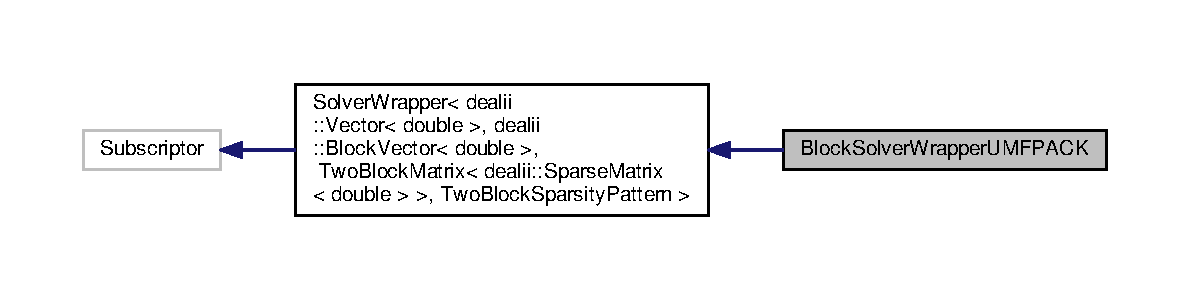
\includegraphics[width=350pt]{class_block_solver_wrapper_u_m_f_p_a_c_k__inherit__graph}
\end{center}
\end{figure}


Collaboration diagram for Block\+Solver\+Wrapper\+U\+M\+F\+P\+A\+CK\+:\nopagebreak
\begin{figure}[H]
\begin{center}
\leavevmode
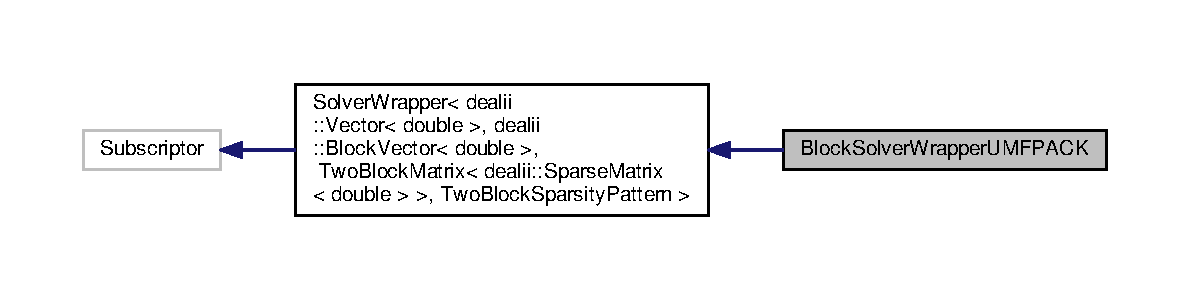
\includegraphics[width=350pt]{class_block_solver_wrapper_u_m_f_p_a_c_k__coll__graph}
\end{center}
\end{figure}
\subsection*{Public Member Functions}
\begin{DoxyCompactItemize}
\item 
virtual void \hyperlink{class_block_solver_wrapper_u_m_f_p_a_c_k_a0d27521861712a3b36cc15845e093df2}{solve} (const \hyperlink{class_two_block_matrix}{Two\+Block\+Matrix}$<$ {\bf dealii\+::\+Sparse\+Matrix}$<$ double $>$$>$ \&K\+\_\+stretched, {\bf dealii\+::\+Vector}$<$ double $>$ \&solution, const {\bf dealii\+::\+Block\+Vector}$<$ double $>$ \&f\+\_\+stretched, const bool symmetric=false)
\end{DoxyCompactItemize}


\subsection{Detailed Description}
A \hyperlink{class_solver_wrapper}{Solver\+Wrapper} for the direct solver from U\+M\+F\+P\+A\+CK for the case of a \hyperlink{class_two_block_matrix}{Two\+Block\+Matrix} using the U\+M\+F\+P\+A\+CK interface of deal.\+II 

\subsection{Member Function Documentation}
\index{Block\+Solver\+Wrapper\+U\+M\+F\+P\+A\+CK@{Block\+Solver\+Wrapper\+U\+M\+F\+P\+A\+CK}!solve@{solve}}
\index{solve@{solve}!Block\+Solver\+Wrapper\+U\+M\+F\+P\+A\+CK@{Block\+Solver\+Wrapper\+U\+M\+F\+P\+A\+CK}}
\subsubsection[{\texorpdfstring{solve(const Two\+Block\+Matrix$<$ dealii\+::\+Sparse\+Matrix$<$ double $>$$>$ \&\+K\+\_\+stretched, dealii\+::\+Vector$<$ double $>$ \&solution, const dealii\+::\+Block\+Vector$<$ double $>$ \&f\+\_\+stretched, const bool symmetric=false)}{solve(const TwoBlockMatrix< dealii::SparseMatrix< double >> &K_stretched, dealii::Vector< double > &solution, const dealii::BlockVector< double > &f_stretched, const bool symmetric=false)}}]{\setlength{\rightskip}{0pt plus 5cm}virtual void Block\+Solver\+Wrapper\+U\+M\+F\+P\+A\+C\+K\+::solve (
\begin{DoxyParamCaption}
\item[{const {\bf Two\+Block\+Matrix}$<$ {\bf dealii\+::\+Sparse\+Matrix}$<$ double $>$$>$ \&}]{K\+\_\+stretched, }
\item[{{\bf dealii\+::\+Vector}$<$ double $>$ \&}]{solution, }
\item[{const {\bf dealii\+::\+Block\+Vector}$<$ double $>$ \&}]{f\+\_\+stretched, }
\item[{const bool}]{symmetric = {\ttfamily false}}
\end{DoxyParamCaption}
)\hspace{0.3cm}{\ttfamily [virtual]}}\hypertarget{class_block_solver_wrapper_u_m_f_p_a_c_k_a0d27521861712a3b36cc15845e093df2}{}\label{class_block_solver_wrapper_u_m_f_p_a_c_k_a0d27521861712a3b36cc15845e093df2}




The solve function for the system of linear equations in the stretched form


\begin{DoxyParams}[1]{Parameters}
\mbox{\tt in}  & {\em K\+\_\+stretched} & The stretched system\+\_\+matrix\\
\hline
\mbox{\tt out}  & {\em solution} & The stretched solution vector\\
\hline
\mbox{\tt in}  & {\em f\+\_\+stretched} & The stretched right hand side vector\\
\hline
\mbox{\tt in}  & {\em symmetric} & A bool indicating whether {\ttfamily system\+\_\+matrix} is symmetric \\
\hline
\end{DoxyParams}


The documentation for this class was generated from the following file\+:\begin{DoxyCompactItemize}
\item 
/home/sst/code/\+Galerkin\+Tools/\+Galerkin\+Tools/include/galerkin\+\_\+tools/\hyperlink{solver__wrapper_8h}{solver\+\_\+wrapper.\+h}\end{DoxyCompactItemize}

\hypertarget{class_block_solver_wrapper_u_m_f_p_a_c_k2}{}\doxysection{Block\+Solver\+Wrapper\+U\+M\+F\+P\+A\+C\+K2 Class Reference}
\label{class_block_solver_wrapper_u_m_f_p_a_c_k2}\index{BlockSolverWrapperUMFPACK2@{BlockSolverWrapperUMFPACK2}}


{\ttfamily \#include $<$solver\+\_\+wrapper.\+h$>$}



Inheritance diagram for Block\+Solver\+Wrapper\+U\+M\+F\+P\+A\+C\+K2\+:\nopagebreak
\begin{figure}[H]
\begin{center}
\leavevmode
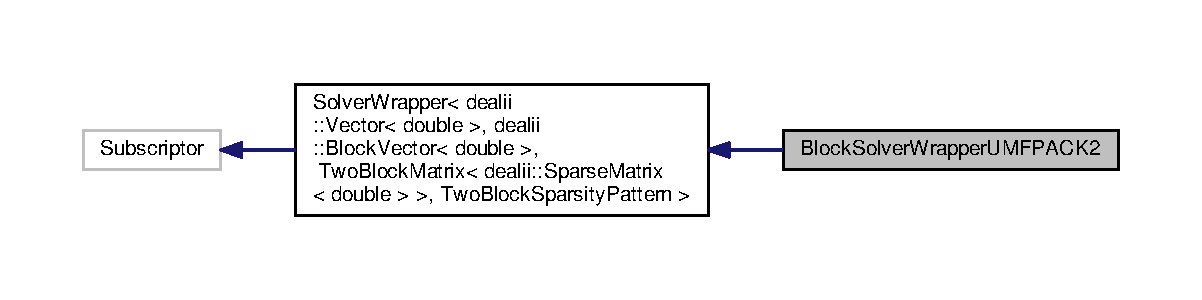
\includegraphics[width=350pt]{class_block_solver_wrapper_u_m_f_p_a_c_k2__inherit__graph}
\end{center}
\end{figure}


Collaboration diagram for Block\+Solver\+Wrapper\+U\+M\+F\+P\+A\+C\+K2\+:\nopagebreak
\begin{figure}[H]
\begin{center}
\leavevmode
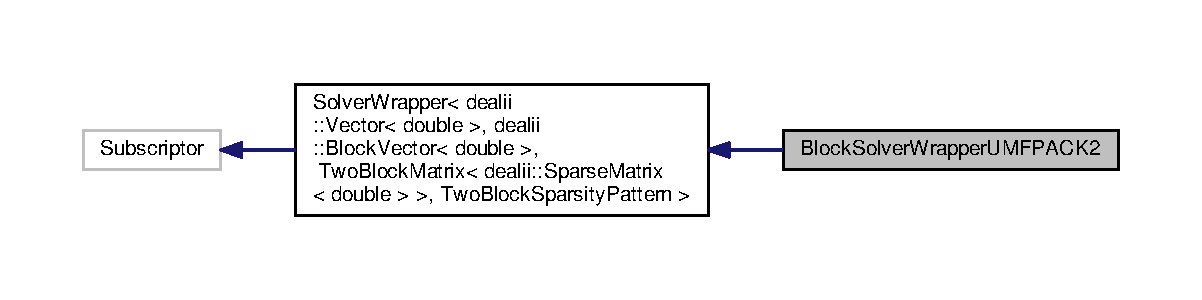
\includegraphics[width=350pt]{class_block_solver_wrapper_u_m_f_p_a_c_k2__coll__graph}
\end{center}
\end{figure}
\doxysubsection*{Public Member Functions}
\begin{DoxyCompactItemize}
\item 
\mbox{\hyperlink{class_block_solver_wrapper_u_m_f_p_a_c_k2_a8f298590602e05af072f1ce4178199f2}{$\sim$\+Block\+Solver\+Wrapper\+U\+M\+F\+P\+A\+C\+K2}} ()
\item 
virtual void \mbox{\hyperlink{class_block_solver_wrapper_u_m_f_p_a_c_k2_a651cb9299e8f368ba7294367260f9759}{solve}} (const \mbox{\hyperlink{class_two_block_matrix}{Two\+Block\+Matrix}}$<$ \textbf{ dealii\+::\+Sparse\+Matrix}$<$ double $>$$>$ \&K\+\_\+stretched, \textbf{ dealii\+::\+Vector}$<$ double $>$ \&solution, const \textbf{ dealii\+::\+Block\+Vector}$<$ double $>$ \&f\+\_\+stretched, const bool symmetric=false)
\item 
\mbox{\hyperlink{class_block_solver_wrapper_u_m_f_p_a_c_k2_aa454139937c8f01d8e893a7e09d3b1a2}{Decl\+Exception2}} (\textbf{ Exc\+U\+M\+F\+P\+A\+C\+K\+Error}, std\+::string, int,$<$$<$ \char`\"{}U\+M\+F\+P\+A\+CK routine \char`\"{}$<$$<$ arg1$<$$<$ \char`\"{} returned error status \char`\"{}$<$$<$ arg2$<$$<$ \char`\"{}.\char`\"{})
\end{DoxyCompactItemize}
\doxysubsection*{Public Attributes}
\begin{DoxyCompactItemize}
\item 
unsigned int \mbox{\hyperlink{class_block_solver_wrapper_u_m_f_p_a_c_k2_a5869a4301c4e7a3ae64aa8998131d8c7}{analyze}} = 0
\item 
unsigned int \mbox{\hyperlink{class_block_solver_wrapper_u_m_f_p_a_c_k2_af78261735f66012f531c3a71c9640d2c}{print\+\_\+level}} = 0
\end{DoxyCompactItemize}
\doxysubsection*{Private Member Functions}
\begin{DoxyCompactItemize}
\item 
void \mbox{\hyperlink{class_block_solver_wrapper_u_m_f_p_a_c_k2_a8df429ef59e02922971ed01dd4780cee}{initialize\+\_\+matrix}} (const \textbf{ Sparse\+Matrix}$<$ double $>$ \&matrix)
\item 
void \mbox{\hyperlink{class_block_solver_wrapper_u_m_f_p_a_c_k2_afc9d5243e71aa81bd391e36976ef5623}{analyze\+\_\+matrix}} ()
\item 
void \mbox{\hyperlink{class_block_solver_wrapper_u_m_f_p_a_c_k2_a1fb479f8089c3b71b2632f0267e6e7ff}{factorize\+\_\+matrix}} ()
\item 
void \mbox{\hyperlink{class_block_solver_wrapper_u_m_f_p_a_c_k2_ac308e6181b48e7e35f533d90a89773f3}{vmult}} (\textbf{ Vector}$<$ double $>$ \&x, const \textbf{ Vector}$<$ double $>$ \&f)
\end{DoxyCompactItemize}
\doxysubsection*{Private Attributes}
\begin{DoxyCompactItemize}
\item 
std\+::vector$<$ double $>$ \mbox{\hyperlink{class_block_solver_wrapper_u_m_f_p_a_c_k2_a295fca0b28991ae43c7bdfb72b5cdcb2}{control}} = std\+::vector$<$double$>$(U\+M\+F\+P\+A\+C\+K\+\_\+\+C\+O\+N\+T\+R\+OL)
\item 
std\+::vector$<$ double $>$ \mbox{\hyperlink{class_block_solver_wrapper_u_m_f_p_a_c_k2_a8dfbe8f5e1f1cf26460ba584b4eb02b6}{info}} = std\+::vector$<$double$>$(U\+M\+F\+P\+A\+C\+K\+\_\+\+I\+N\+FO)
\item 
unsigned int \mbox{\hyperlink{class_block_solver_wrapper_u_m_f_p_a_c_k2_a85d397826a36330bf3602d510acdd8d4}{N}}
\item 
void $\ast$ \mbox{\hyperlink{class_block_solver_wrapper_u_m_f_p_a_c_k2_a399387c1717404d92ed721fc31767f55}{symbolic\+\_\+decomposition}} = nullptr
\item 
void $\ast$ \mbox{\hyperlink{class_block_solver_wrapper_u_m_f_p_a_c_k2_ac3a439162324f36f5162439c075d02eb}{numeric\+\_\+decomposition}} = nullptr
\item 
std\+::vector$<$ Suite\+Sparse\+\_\+long $>$ \mbox{\hyperlink{class_block_solver_wrapper_u_m_f_p_a_c_k2_a18e53f152f97e51caab8dcf3efd5eaf1}{Ap}}
\item 
std\+::vector$<$ Suite\+Sparse\+\_\+long $>$ \mbox{\hyperlink{class_block_solver_wrapper_u_m_f_p_a_c_k2_a088fc386567b26c63b8d1a25a9319c75}{Ai}}
\item 
std\+::vector$<$ double $>$ \mbox{\hyperlink{class_block_solver_wrapper_u_m_f_p_a_c_k2_a57a4f7722dbbdd1ec2efa416f1cbb47c}{Ax}}
\end{DoxyCompactItemize}


\doxysubsection{Detailed Description}
A \mbox{\hyperlink{class_solver_wrapper}{Solver\+Wrapper}} for the direct solver from U\+M\+F\+P\+A\+CK using directly the interface to U\+M\+F\+P\+A\+CK (this allows for more flexibility of the solver compared to \mbox{\hyperlink{class_block_solver_wrapper_u_m_f_p_a_c_k}{Block\+Solver\+Wrapper\+U\+M\+F\+P\+A\+CK}}, which uses the deal.\+II interface to U\+M\+F\+P\+A\+CK)

\begin{DoxyNote}{Note}
U\+M\+F\+P\+A\+CK has its own license, independent of that of Galerkin\+Tools. If you want to use U\+M\+F\+P\+A\+CK you have to accept that license.
\end{DoxyNote}
Code partially copied over from deal.\+II 

\doxysubsection{Constructor \& Destructor Documentation}
\mbox{\Hypertarget{class_block_solver_wrapper_u_m_f_p_a_c_k2_a8f298590602e05af072f1ce4178199f2}\label{class_block_solver_wrapper_u_m_f_p_a_c_k2_a8f298590602e05af072f1ce4178199f2}} 
\index{BlockSolverWrapperUMFPACK2@{BlockSolverWrapperUMFPACK2}!````~BlockSolverWrapperUMFPACK2@{$\sim$BlockSolverWrapperUMFPACK2}}
\index{````~BlockSolverWrapperUMFPACK2@{$\sim$BlockSolverWrapperUMFPACK2}!BlockSolverWrapperUMFPACK2@{BlockSolverWrapperUMFPACK2}}
\doxysubsubsection{\texorpdfstring{$\sim$BlockSolverWrapperUMFPACK2()}{~BlockSolverWrapperUMFPACK2()}}
{\footnotesize\ttfamily Block\+Solver\+Wrapper\+U\+M\+F\+P\+A\+C\+K2\+::$\sim$\+Block\+Solver\+Wrapper\+U\+M\+F\+P\+A\+C\+K2 (\begin{DoxyParamCaption}{ }\end{DoxyParamCaption})}

Destructor. 

\doxysubsection{Member Function Documentation}
\mbox{\Hypertarget{class_block_solver_wrapper_u_m_f_p_a_c_k2_afc9d5243e71aa81bd391e36976ef5623}\label{class_block_solver_wrapper_u_m_f_p_a_c_k2_afc9d5243e71aa81bd391e36976ef5623}} 
\index{BlockSolverWrapperUMFPACK2@{BlockSolverWrapperUMFPACK2}!analyze\_matrix@{analyze\_matrix}}
\index{analyze\_matrix@{analyze\_matrix}!BlockSolverWrapperUMFPACK2@{BlockSolverWrapperUMFPACK2}}
\doxysubsubsection{\texorpdfstring{analyze\_matrix()}{analyze\_matrix()}}
{\footnotesize\ttfamily void Block\+Solver\+Wrapper\+U\+M\+F\+P\+A\+C\+K2\+::analyze\+\_\+matrix (\begin{DoxyParamCaption}{ }\end{DoxyParamCaption})\hspace{0.3cm}{\ttfamily [private]}}

This function analyses the given matrix and sets up \mbox{\hyperlink{class_block_solver_wrapper_u_m_f_p_a_c_k2_a399387c1717404d92ed721fc31767f55}{Block\+Solver\+Wrapper\+U\+M\+F\+P\+A\+C\+K2\+::symbolic\+\_\+decomposition}}. Whether this function does anything depends upon the value of \mbox{\hyperlink{class_block_solver_wrapper_u_m_f_p_a_c_k2_a5869a4301c4e7a3ae64aa8998131d8c7}{Block\+Solver\+Wrapper\+U\+M\+F\+P\+A\+C\+K2\+::analyze}}. \mbox{\Hypertarget{class_block_solver_wrapper_u_m_f_p_a_c_k2_aa454139937c8f01d8e893a7e09d3b1a2}\label{class_block_solver_wrapper_u_m_f_p_a_c_k2_aa454139937c8f01d8e893a7e09d3b1a2}} 
\index{BlockSolverWrapperUMFPACK2@{BlockSolverWrapperUMFPACK2}!DeclException2@{DeclException2}}
\index{DeclException2@{DeclException2}!BlockSolverWrapperUMFPACK2@{BlockSolverWrapperUMFPACK2}}
\doxysubsubsection{\texorpdfstring{DeclException2()}{DeclException2()}}
{\footnotesize\ttfamily Block\+Solver\+Wrapper\+U\+M\+F\+P\+A\+C\+K2\+::\+Decl\+Exception2 (\begin{DoxyParamCaption}\item[{\textbf{ Exc\+U\+M\+F\+P\+A\+C\+K\+Error}}]{,  }\item[{std\+::string}]{,  }\item[{int}]{,  }\item[{$<$$<$ \char`\"{}U\+M\+F\+P\+A\+CK routine \char`\"{}$<$$<$ arg1$<$$<$ \char`\"{} returned error status \char`\"{}$<$$<$ arg2$<$$<$ \char`\"{}.\char`\"{}}]{ }\end{DoxyParamCaption})}

\mbox{\Hypertarget{class_block_solver_wrapper_u_m_f_p_a_c_k2_a1fb479f8089c3b71b2632f0267e6e7ff}\label{class_block_solver_wrapper_u_m_f_p_a_c_k2_a1fb479f8089c3b71b2632f0267e6e7ff}} 
\index{BlockSolverWrapperUMFPACK2@{BlockSolverWrapperUMFPACK2}!factorize\_matrix@{factorize\_matrix}}
\index{factorize\_matrix@{factorize\_matrix}!BlockSolverWrapperUMFPACK2@{BlockSolverWrapperUMFPACK2}}
\doxysubsubsection{\texorpdfstring{factorize\_matrix()}{factorize\_matrix()}}
{\footnotesize\ttfamily void Block\+Solver\+Wrapper\+U\+M\+F\+P\+A\+C\+K2\+::factorize\+\_\+matrix (\begin{DoxyParamCaption}{ }\end{DoxyParamCaption})\hspace{0.3cm}{\ttfamily [private]}}

This function factorizes the matrix. The result is available from \mbox{\hyperlink{class_block_solver_wrapper_u_m_f_p_a_c_k2_ac3a439162324f36f5162439c075d02eb}{Block\+Solver\+Wrapper\+U\+M\+F\+P\+A\+C\+K2\+::numeric\+\_\+decomposition}}. \mbox{\Hypertarget{class_block_solver_wrapper_u_m_f_p_a_c_k2_a8df429ef59e02922971ed01dd4780cee}\label{class_block_solver_wrapper_u_m_f_p_a_c_k2_a8df429ef59e02922971ed01dd4780cee}} 
\index{BlockSolverWrapperUMFPACK2@{BlockSolverWrapperUMFPACK2}!initialize\_matrix@{initialize\_matrix}}
\index{initialize\_matrix@{initialize\_matrix}!BlockSolverWrapperUMFPACK2@{BlockSolverWrapperUMFPACK2}}
\doxysubsubsection{\texorpdfstring{initialize\_matrix()}{initialize\_matrix()}}
{\footnotesize\ttfamily void Block\+Solver\+Wrapper\+U\+M\+F\+P\+A\+C\+K2\+::initialize\+\_\+matrix (\begin{DoxyParamCaption}\item[{const \textbf{ Sparse\+Matrix}$<$ double $>$ \&}]{matrix }\end{DoxyParamCaption})\hspace{0.3cm}{\ttfamily [private]}}

Sets the data structures storing the matrix up (\mbox{\hyperlink{class_block_solver_wrapper_u_m_f_p_a_c_k2_a18e53f152f97e51caab8dcf3efd5eaf1}{Block\+Solver\+Wrapper\+U\+M\+F\+P\+A\+C\+K2\+::\+Ap}}, \mbox{\hyperlink{class_block_solver_wrapper_u_m_f_p_a_c_k2_a088fc386567b26c63b8d1a25a9319c75}{Block\+Solver\+Wrapper\+U\+M\+F\+P\+A\+C\+K2\+::\+Ai}}, \mbox{\hyperlink{class_block_solver_wrapper_u_m_f_p_a_c_k2_a57a4f7722dbbdd1ec2efa416f1cbb47c}{Block\+Solver\+Wrapper\+U\+M\+F\+P\+A\+C\+K2\+::\+Ax}}).

Also sets up the control parameters for the U\+M\+F\+P\+A\+CK routines


\begin{DoxyParams}[1]{Parameters}
\mbox{\texttt{ in}}  & {\em matrix} & The matrix A \\
\hline
\end{DoxyParams}
\mbox{\Hypertarget{class_block_solver_wrapper_u_m_f_p_a_c_k2_a651cb9299e8f368ba7294367260f9759}\label{class_block_solver_wrapper_u_m_f_p_a_c_k2_a651cb9299e8f368ba7294367260f9759}} 
\index{BlockSolverWrapperUMFPACK2@{BlockSolverWrapperUMFPACK2}!solve@{solve}}
\index{solve@{solve}!BlockSolverWrapperUMFPACK2@{BlockSolverWrapperUMFPACK2}}
\doxysubsubsection{\texorpdfstring{solve()}{solve()}}
{\footnotesize\ttfamily virtual void Block\+Solver\+Wrapper\+U\+M\+F\+P\+A\+C\+K2\+::solve (\begin{DoxyParamCaption}\item[{const \mbox{\hyperlink{class_two_block_matrix}{Two\+Block\+Matrix}}$<$ \textbf{ dealii\+::\+Sparse\+Matrix}$<$ double $>$$>$ \&}]{K\+\_\+stretched,  }\item[{\textbf{ dealii\+::\+Vector}$<$ double $>$ \&}]{solution,  }\item[{const \textbf{ dealii\+::\+Block\+Vector}$<$ double $>$ \&}]{f\+\_\+stretched,  }\item[{const bool}]{symmetric = {\ttfamily false} }\end{DoxyParamCaption})\hspace{0.3cm}{\ttfamily [virtual]}}





The solve function for the system of linear equations in the stretched form


\begin{DoxyParams}[1]{Parameters}
\mbox{\texttt{ in}}  & {\em K\+\_\+stretched} & The stretched system\+\_\+matrix\\
\hline
\mbox{\texttt{ out}}  & {\em solution} & The stretched solution vector\\
\hline
\mbox{\texttt{ in}}  & {\em f\+\_\+stretched} & The stretched right hand side vector\\
\hline
\mbox{\texttt{ in}}  & {\em symmetric} & A bool indicating whether {\ttfamily system\+\_\+matrix} is symmetric \\
\hline
\end{DoxyParams}
\mbox{\Hypertarget{class_block_solver_wrapper_u_m_f_p_a_c_k2_ac308e6181b48e7e35f533d90a89773f3}\label{class_block_solver_wrapper_u_m_f_p_a_c_k2_ac308e6181b48e7e35f533d90a89773f3}} 
\index{BlockSolverWrapperUMFPACK2@{BlockSolverWrapperUMFPACK2}!vmult@{vmult}}
\index{vmult@{vmult}!BlockSolverWrapperUMFPACK2@{BlockSolverWrapperUMFPACK2}}
\doxysubsubsection{\texorpdfstring{vmult()}{vmult()}}
{\footnotesize\ttfamily void Block\+Solver\+Wrapper\+U\+M\+F\+P\+A\+C\+K2\+::vmult (\begin{DoxyParamCaption}\item[{\textbf{ Vector}$<$ double $>$ \&}]{x,  }\item[{const \textbf{ Vector}$<$ double $>$ \&}]{f }\end{DoxyParamCaption})\hspace{0.3cm}{\ttfamily [private]}}

Multiply the inverse of A by {\ttfamily f} and store the result into {\ttfamily x}. I.\+e., solve Ax=f for x. This uses the factors computed by \mbox{\hyperlink{class_block_solver_wrapper_u_m_f_p_a_c_k2_a1fb479f8089c3b71b2632f0267e6e7ff}{Block\+Solver\+Wrapper\+U\+M\+F\+P\+A\+C\+K2\+::factorize\+\_\+matrix()}}.


\begin{DoxyParams}[1]{Parameters}
\mbox{\texttt{ out}}  & {\em x} & solution \\
\hline
\mbox{\texttt{ in}}  & {\em f} & rhs \\
\hline
\end{DoxyParams}


\doxysubsection{Member Data Documentation}
\mbox{\Hypertarget{class_block_solver_wrapper_u_m_f_p_a_c_k2_a088fc386567b26c63b8d1a25a9319c75}\label{class_block_solver_wrapper_u_m_f_p_a_c_k2_a088fc386567b26c63b8d1a25a9319c75}} 
\index{BlockSolverWrapperUMFPACK2@{BlockSolverWrapperUMFPACK2}!Ai@{Ai}}
\index{Ai@{Ai}!BlockSolverWrapperUMFPACK2@{BlockSolverWrapperUMFPACK2}}
\doxysubsubsection{\texorpdfstring{Ai}{Ai}}
{\footnotesize\ttfamily std\+::vector$<$Suite\+Sparse\+\_\+long$>$ Block\+Solver\+Wrapper\+U\+M\+F\+P\+A\+C\+K2\+::\+Ai\hspace{0.3cm}{\ttfamily [private]}}

Array storing the column indices of non-\/zero entries of A \mbox{\Hypertarget{class_block_solver_wrapper_u_m_f_p_a_c_k2_a5869a4301c4e7a3ae64aa8998131d8c7}\label{class_block_solver_wrapper_u_m_f_p_a_c_k2_a5869a4301c4e7a3ae64aa8998131d8c7}} 
\index{BlockSolverWrapperUMFPACK2@{BlockSolverWrapperUMFPACK2}!analyze@{analyze}}
\index{analyze@{analyze}!BlockSolverWrapperUMFPACK2@{BlockSolverWrapperUMFPACK2}}
\doxysubsubsection{\texorpdfstring{analyze}{analyze}}
{\footnotesize\ttfamily unsigned int Block\+Solver\+Wrapper\+U\+M\+F\+P\+A\+C\+K2\+::analyze = 0}

Key indicating when to analyze the matrix structure\+:~\newline
 0 -\/ before each factorization (default)~\newline
 1 -\/ only before the next factorization (afterwards, \mbox{\hyperlink{class_block_solver_wrapper_u_m_f_p_a_c_k2_a5869a4301c4e7a3ae64aa8998131d8c7}{Block\+Solver\+Wrapper\+U\+M\+F\+P\+A\+C\+K2\+::analyze}} will be set to 2)~\newline
 $>$=2 -\/ do not recompute

\begin{DoxyWarning}{Warning}
The user must ensure that \mbox{\hyperlink{class_block_solver_wrapper_u_m_f_p_a_c_k2_a5869a4301c4e7a3ae64aa8998131d8c7}{Block\+Solver\+Wrapper\+U\+M\+F\+P\+A\+C\+K2\+::analyze}}=0 or \mbox{\hyperlink{class_block_solver_wrapper_u_m_f_p_a_c_k2_a5869a4301c4e7a3ae64aa8998131d8c7}{Block\+Solver\+Wrapper\+U\+M\+F\+P\+A\+C\+K2\+::analyze}}=1 whenever the sparsity pattern of the matrix has changed (or during the first call). Currently, no internal checking is performed. 
\end{DoxyWarning}
\mbox{\Hypertarget{class_block_solver_wrapper_u_m_f_p_a_c_k2_a18e53f152f97e51caab8dcf3efd5eaf1}\label{class_block_solver_wrapper_u_m_f_p_a_c_k2_a18e53f152f97e51caab8dcf3efd5eaf1}} 
\index{BlockSolverWrapperUMFPACK2@{BlockSolverWrapperUMFPACK2}!Ap@{Ap}}
\index{Ap@{Ap}!BlockSolverWrapperUMFPACK2@{BlockSolverWrapperUMFPACK2}}
\doxysubsubsection{\texorpdfstring{Ap}{Ap}}
{\footnotesize\ttfamily std\+::vector$<$Suite\+Sparse\+\_\+long$>$ Block\+Solver\+Wrapper\+U\+M\+F\+P\+A\+C\+K2\+::\+Ap\hspace{0.3cm}{\ttfamily [private]}}

Array saying which row starts where in \mbox{\hyperlink{class_block_solver_wrapper_u_m_f_p_a_c_k2_a088fc386567b26c63b8d1a25a9319c75}{Block\+Solver\+Wrapper\+U\+M\+F\+P\+A\+C\+K2\+::\+Ai}} \mbox{\Hypertarget{class_block_solver_wrapper_u_m_f_p_a_c_k2_a57a4f7722dbbdd1ec2efa416f1cbb47c}\label{class_block_solver_wrapper_u_m_f_p_a_c_k2_a57a4f7722dbbdd1ec2efa416f1cbb47c}} 
\index{BlockSolverWrapperUMFPACK2@{BlockSolverWrapperUMFPACK2}!Ax@{Ax}}
\index{Ax@{Ax}!BlockSolverWrapperUMFPACK2@{BlockSolverWrapperUMFPACK2}}
\doxysubsubsection{\texorpdfstring{Ax}{Ax}}
{\footnotesize\ttfamily std\+::vector$<$double$>$ Block\+Solver\+Wrapper\+U\+M\+F\+P\+A\+C\+K2\+::\+Ax\hspace{0.3cm}{\ttfamily [private]}}

Array storing the numerical values of the non-\/zero entries of the matrix A \mbox{\Hypertarget{class_block_solver_wrapper_u_m_f_p_a_c_k2_a295fca0b28991ae43c7bdfb72b5cdcb2}\label{class_block_solver_wrapper_u_m_f_p_a_c_k2_a295fca0b28991ae43c7bdfb72b5cdcb2}} 
\index{BlockSolverWrapperUMFPACK2@{BlockSolverWrapperUMFPACK2}!control@{control}}
\index{control@{control}!BlockSolverWrapperUMFPACK2@{BlockSolverWrapperUMFPACK2}}
\doxysubsubsection{\texorpdfstring{control}{control}}
{\footnotesize\ttfamily std\+::vector$<$double$>$ Block\+Solver\+Wrapper\+U\+M\+F\+P\+A\+C\+K2\+::control = std\+::vector$<$double$>$(U\+M\+F\+P\+A\+C\+K\+\_\+\+C\+O\+N\+T\+R\+OL)\hspace{0.3cm}{\ttfamily [private]}}

Control array for the solver routines. \mbox{\Hypertarget{class_block_solver_wrapper_u_m_f_p_a_c_k2_a8dfbe8f5e1f1cf26460ba584b4eb02b6}\label{class_block_solver_wrapper_u_m_f_p_a_c_k2_a8dfbe8f5e1f1cf26460ba584b4eb02b6}} 
\index{BlockSolverWrapperUMFPACK2@{BlockSolverWrapperUMFPACK2}!info@{info}}
\index{info@{info}!BlockSolverWrapperUMFPACK2@{BlockSolverWrapperUMFPACK2}}
\doxysubsubsection{\texorpdfstring{info}{info}}
{\footnotesize\ttfamily std\+::vector$<$double$>$ Block\+Solver\+Wrapper\+U\+M\+F\+P\+A\+C\+K2\+::info = std\+::vector$<$double$>$(U\+M\+F\+P\+A\+C\+K\+\_\+\+I\+N\+FO)\hspace{0.3cm}{\ttfamily [private]}}

Info array for the solver routines. \mbox{\Hypertarget{class_block_solver_wrapper_u_m_f_p_a_c_k2_a85d397826a36330bf3602d510acdd8d4}\label{class_block_solver_wrapper_u_m_f_p_a_c_k2_a85d397826a36330bf3602d510acdd8d4}} 
\index{BlockSolverWrapperUMFPACK2@{BlockSolverWrapperUMFPACK2}!N@{N}}
\index{N@{N}!BlockSolverWrapperUMFPACK2@{BlockSolverWrapperUMFPACK2}}
\doxysubsubsection{\texorpdfstring{N}{N}}
{\footnotesize\ttfamily unsigned int Block\+Solver\+Wrapper\+U\+M\+F\+P\+A\+C\+K2\+::N\hspace{0.3cm}{\ttfamily [private]}}

The size of the matrix A of the \mbox{\hyperlink{class_two_block_matrix}{Two\+Block\+Matrix}} \mbox{\Hypertarget{class_block_solver_wrapper_u_m_f_p_a_c_k2_ac3a439162324f36f5162439c075d02eb}\label{class_block_solver_wrapper_u_m_f_p_a_c_k2_ac3a439162324f36f5162439c075d02eb}} 
\index{BlockSolverWrapperUMFPACK2@{BlockSolverWrapperUMFPACK2}!numeric\_decomposition@{numeric\_decomposition}}
\index{numeric\_decomposition@{numeric\_decomposition}!BlockSolverWrapperUMFPACK2@{BlockSolverWrapperUMFPACK2}}
\doxysubsubsection{\texorpdfstring{numeric\_decomposition}{numeric\_decomposition}}
{\footnotesize\ttfamily void$\ast$ Block\+Solver\+Wrapper\+U\+M\+F\+P\+A\+C\+K2\+::numeric\+\_\+decomposition = nullptr\hspace{0.3cm}{\ttfamily [private]}}

U\+M\+F\+P\+A\+CK numeric decomposition of A \mbox{\Hypertarget{class_block_solver_wrapper_u_m_f_p_a_c_k2_af78261735f66012f531c3a71c9640d2c}\label{class_block_solver_wrapper_u_m_f_p_a_c_k2_af78261735f66012f531c3a71c9640d2c}} 
\index{BlockSolverWrapperUMFPACK2@{BlockSolverWrapperUMFPACK2}!print\_level@{print\_level}}
\index{print\_level@{print\_level}!BlockSolverWrapperUMFPACK2@{BlockSolverWrapperUMFPACK2}}
\doxysubsubsection{\texorpdfstring{print\_level}{print\_level}}
{\footnotesize\ttfamily unsigned int Block\+Solver\+Wrapper\+U\+M\+F\+P\+A\+C\+K2\+::print\+\_\+level = 0}

level of diagnostic printing\+:~\newline
 0\+: no output~\newline
 1\+: error messages only~\newline
 2 or more\+: print status, whether or not an error occurred~\newline
 4 or more\+: also print the U\+M\+F\+P\+A\+CK Copyright~\newline
 6 or more\+: also print the U\+M\+F\+P\+A\+CK License \mbox{\Hypertarget{class_block_solver_wrapper_u_m_f_p_a_c_k2_a399387c1717404d92ed721fc31767f55}\label{class_block_solver_wrapper_u_m_f_p_a_c_k2_a399387c1717404d92ed721fc31767f55}} 
\index{BlockSolverWrapperUMFPACK2@{BlockSolverWrapperUMFPACK2}!symbolic\_decomposition@{symbolic\_decomposition}}
\index{symbolic\_decomposition@{symbolic\_decomposition}!BlockSolverWrapperUMFPACK2@{BlockSolverWrapperUMFPACK2}}
\doxysubsubsection{\texorpdfstring{symbolic\_decomposition}{symbolic\_decomposition}}
{\footnotesize\ttfamily void$\ast$ Block\+Solver\+Wrapper\+U\+M\+F\+P\+A\+C\+K2\+::symbolic\+\_\+decomposition = nullptr\hspace{0.3cm}{\ttfamily [private]}}

U\+M\+F\+P\+A\+CK symbolic decomposition of A 

The documentation for this class was generated from the following file\+:\begin{DoxyCompactItemize}
\item 
/home/sst/code/\+Galerkin\+Tools/\+Galerkin\+Tools/include/galerkin\+\_\+tools/\mbox{\hyperlink{solver__wrapper_8h}{solver\+\_\+wrapper.\+h}}\end{DoxyCompactItemize}

\hypertarget{class_dependent_field}{}\doxysection{Dependent\+Field$<$ dim, spacedim $>$ Class Template Reference}
\label{class_dependent_field}\index{DependentField$<$ dim, spacedim $>$@{DependentField$<$ dim, spacedim $>$}}


{\ttfamily \#include $<$dependent\+\_\+field.\+h$>$}

\doxysubsection*{Public Member Functions}
\begin{DoxyCompactItemize}
\item 
\mbox{\hyperlink{class_dependent_field_a5a47b8f5b0e51b29bf6f3ca6e18fda9c}{Dependent\+Field}} (const std\+::string \mbox{\hyperlink{class_dependent_field_a698b255f131279d1edb97b3c525153a0}{name}})
\item 
void \mbox{\hyperlink{class_dependent_field_a0726cab14197769ad07bd8f071e395ea}{add\+\_\+term}} (double coefficient, const \mbox{\hyperlink{class_independent_field}{Independent\+Field}}$<$ dim, spacedim $>$ \&independent\+\_\+field, const unsigned int component=0, const std\+::vector$<$ unsigned int $>$ derivatives=std\+::vector$<$ unsigned int $>$())
\item 
void \mbox{\hyperlink{class_dependent_field_a852ed477f6ee71ad85a6690d4a5e56fe}{add\+\_\+term}} (double coefficient, const \mbox{\hyperlink{class_independent_field}{Independent\+Field}}$<$ dim+1, spacedim $>$ \&independent\+\_\+field, const unsigned int component, const std\+::vector$<$ unsigned int $>$ derivatives, const \mbox{\hyperlink{triangulation__system_8h_a44f3c00e36c1d6e3c389ae693c09b435}{Interface\+Side}} side)
\item 
void \mbox{\hyperlink{class_dependent_field_acb8979c891a45ed7326eb47df41c0129}{add\+\_\+term}} (double coefficient, const \mbox{\hyperlink{class_independent_field}{Independent\+Field}}$<$ dim+1, spacedim $>$ \&independent\+\_\+field, const unsigned int component, const \mbox{\hyperlink{triangulation__system_8h_a44f3c00e36c1d6e3c389ae693c09b435}{Interface\+Side}} side)
\item 
void \mbox{\hyperlink{class_dependent_field_a1aaaf072334d4e06640383ae81766a39}{add\+\_\+term}} (double coefficient, const \mbox{\hyperlink{class_independent_field}{Independent\+Field}}$<$ dim, spacedim $>$ \&independent\+\_\+field, const unsigned int component, const unsigned int derivative)
\item 
void \mbox{\hyperlink{class_dependent_field_a43de305294f94c38c88fa4768b3f0155}{add\+\_\+term}} (double coefficient, const \mbox{\hyperlink{class_independent_field}{Independent\+Field}}$<$ dim+1, spacedim $>$ \&independent\+\_\+field, const unsigned int component, const unsigned int derivative, const \mbox{\hyperlink{triangulation__system_8h_a44f3c00e36c1d6e3c389ae693c09b435}{Interface\+Side}} side)
\item 
void \mbox{\hyperlink{class_dependent_field_adf9e4863ca954a9fa70c57aef68849f8}{add\+\_\+term}} (double coefficient, const \mbox{\hyperlink{class_independent_field}{Independent\+Field}}$<$ 0, spacedim $>$ \&independent\+\_\+field)
\item 
void \mbox{\hyperlink{class_dependent_field_a72196bff18c2c28a1e811877e739f4ee}{add\+\_\+term}} (double \mbox{\hyperlink{class_dependent_field_a32b37c78e04a16b6b606442f156c8ca9}{constant}})
\item 
const std\+::set$<$ \mbox{\hyperlink{class_dependent_field_term}{Dependent\+Field\+Term}}$<$ dim, spacedim $>$, \mbox{\hyperlink{struct_dependent_field_comparator_without_coefficient}{Dependent\+Field\+Comparator\+Without\+Coefficient}}$<$ dim, spacedim $>$ $>$ \& \mbox{\hyperlink{class_dependent_field_a01793fd56b83754bec50e9d4e0c94cae}{get\+\_\+terms\+\_\+interface}} () const
\item 
const std\+::set$<$ \mbox{\hyperlink{class_dependent_field_term}{Dependent\+Field\+Term}}$<$ dim+1, spacedim $>$, \mbox{\hyperlink{struct_dependent_field_comparator_without_coefficient}{Dependent\+Field\+Comparator\+Without\+Coefficient}}$<$ dim+1, spacedim $>$ $>$ \& \mbox{\hyperlink{class_dependent_field_aa88f72409a02de7505ff5ac5d694ed36}{get\+\_\+terms\+\_\+neighbor}} (const \mbox{\hyperlink{triangulation__system_8h_a44f3c00e36c1d6e3c389ae693c09b435}{Interface\+Side}} side) const
\item 
const std\+::set$<$ \mbox{\hyperlink{class_dependent_field_term}{Dependent\+Field\+Term}}$<$ 0, spacedim $>$, \mbox{\hyperlink{struct_dependent_field_comparator_without_coefficient}{Dependent\+Field\+Comparator\+Without\+Coefficient}}$<$ 0, spacedim $>$ $>$ \& \mbox{\hyperlink{class_dependent_field_a89fed0663944d7f392ddd4b75bcb60a8}{get\+\_\+terms\+\_\+independent\+\_\+scalars}} () const
\item 
double \mbox{\hyperlink{class_dependent_field_a213c5de7c4726eb823590de0510f1ff1}{get\+\_\+constant}} () const
\item 
std\+::set$<$ const \mbox{\hyperlink{class_independent_field}{Independent\+Field}}$<$ dim, spacedim $>$ $\ast$ $>$ \mbox{\hyperlink{class_dependent_field_a33760e356c5704614ed8cf7c532b4de6}{get\+\_\+independent\+\_\+fields\+\_\+interface}} () const
\item 
std\+::set$<$ const \mbox{\hyperlink{class_independent_field}{Independent\+Field}}$<$ dim+1, spacedim $>$ $\ast$ $>$ \mbox{\hyperlink{class_dependent_field_ac12fccee9603f2cf36990af16d8da604}{get\+\_\+independent\+\_\+fields\+\_\+neighbors}} () const
\item 
std\+::set$<$ const \mbox{\hyperlink{class_independent_field}{Independent\+Field}}$<$ 0, spacedim $>$ $\ast$ $>$ \mbox{\hyperlink{class_dependent_field_a15eb8101d33f2f09ada4cdf2cde73ad7}{get\+\_\+independent\+\_\+scalars}} () const
\item 
void \mbox{\hyperlink{class_dependent_field_adf0ad81e2d7b609b7dfde60a77f92a20}{print}} () const
\item 
bool \mbox{\hyperlink{class_dependent_field_aabc31c47b3f6cb69da28758d9672d8d8}{get\+\_\+is\+\_\+local}} () const
\item 
bool \mbox{\hyperlink{class_dependent_field_aa16f1559eca5060b0877dc3ec00cc552}{get\+\_\+is\+\_\+locally\+\_\+eliminated}} () const
\item 
bool \mbox{\hyperlink{class_dependent_field_a1c56c4e18d320e9c402f3adde546c681}{operator$<$}} (const \mbox{\hyperlink{class_dependent_field}{Dependent\+Field}} \&dependent\+\_\+field\+\_\+2) const
\item 
bool \mbox{\hyperlink{class_dependent_field_a808b18c7b0fc7c05204aed47b1509ce4}{operator==}} (const \mbox{\hyperlink{class_dependent_field}{Dependent\+Field}} \&dependent\+\_\+field\+\_\+2) const
\end{DoxyCompactItemize}
\doxysubsection*{Public Attributes}
\begin{DoxyCompactItemize}
\item 
const std\+::string \mbox{\hyperlink{class_dependent_field_a698b255f131279d1edb97b3c525153a0}{name}}
\end{DoxyCompactItemize}
\doxysubsection*{Private Attributes}
\begin{DoxyCompactItemize}
\item 
std\+::set$<$ \mbox{\hyperlink{class_dependent_field_term}{Dependent\+Field\+Term}}$<$ dim, spacedim $>$, \mbox{\hyperlink{struct_dependent_field_comparator_without_coefficient}{Dependent\+Field\+Comparator\+Without\+Coefficient}}$<$ dim, spacedim $>$ $>$ \mbox{\hyperlink{class_dependent_field_a463f490ef397b9b65112c94932afcd5c}{terms\+\_\+interface}}
\item 
std\+::set$<$ \mbox{\hyperlink{class_dependent_field_term}{Dependent\+Field\+Term}}$<$ dim+1, spacedim $>$, \mbox{\hyperlink{struct_dependent_field_comparator_without_coefficient}{Dependent\+Field\+Comparator\+Without\+Coefficient}}$<$ dim+1, spacedim $>$ $>$ \mbox{\hyperlink{class_dependent_field_a3f7812cd53686afce899438ae999999a}{terms\+\_\+neighbor\+\_\+plus}}
\item 
std\+::set$<$ \mbox{\hyperlink{class_dependent_field_term}{Dependent\+Field\+Term}}$<$ dim+1, spacedim $>$, \mbox{\hyperlink{struct_dependent_field_comparator_without_coefficient}{Dependent\+Field\+Comparator\+Without\+Coefficient}}$<$ dim+1, spacedim $>$ $>$ \mbox{\hyperlink{class_dependent_field_a406b6490dcd17d80737500184131a3e7}{terms\+\_\+neighbor\+\_\+minus}}
\item 
std\+::set$<$ \mbox{\hyperlink{class_dependent_field_term}{Dependent\+Field\+Term}}$<$ 0, spacedim $>$, \mbox{\hyperlink{struct_dependent_field_comparator_without_coefficient}{Dependent\+Field\+Comparator\+Without\+Coefficient}}$<$ 0, spacedim $>$ $>$ \mbox{\hyperlink{class_dependent_field_a642147ff57d5412554508f293182c649}{terms\+\_\+independent\+\_\+scalars}}
\item 
double \mbox{\hyperlink{class_dependent_field_a32b37c78e04a16b6b606442f156c8ca9}{constant}} = 0.\+0
\item 
bool \mbox{\hyperlink{class_dependent_field_aacdabff2601b1f0efcdce7a4413b47bc}{is\+\_\+local}} = false
\item 
bool \mbox{\hyperlink{class_dependent_field_a9c41e749b67a39b68a37ad9d893fb14d}{is\+\_\+locally\+\_\+eliminated}} = false
\end{DoxyCompactItemize}


\doxysubsection{Detailed Description}
\subsubsection*{template$<$unsigned int dim, unsigned int spacedim$>$\newline
class Dependent\+Field$<$ dim, spacedim $>$}

This class is used to define an interface related dependent field $e^\Sigma_\nu$ ( $\nu \in N=\left\{1 \hdots N^\mathrm{e,\Sigma}\right\}$) according to \begin{equation*} \begin{split} e^\Sigma_\nu &= \sum_{\eta \in H} \left[ a^\Sigma_{\nu\eta} u^\Sigma_\eta + b^\Sigma_{\nu\eta i} \dfrac{\partial u^\Sigma_\eta}{\partial x_i} \right]\\ & + \sum_{\epsilon \in E} \left[ a^+_{\nu\epsilon} (u^\Omega_\epsilon)^+ + b^+_{\nu\epsilon i} \left(\dfrac{\partial u^\Omega_\epsilon}{\partial x_i}\right)^+ \right]\\ & + \sum_{\epsilon \in E} \left[ a^-_{\nu\epsilon} (u^\Omega_\epsilon)^- + b^-_{\nu\epsilon i} \left(\dfrac{\partial u^\Omega_\epsilon}{\partial x_i}\right)^- \right]\\ & + \sum_{\iota \in I}c^\Sigma_{\nu\iota} C_\iota + d^\Sigma_\nu. \end{split} \end{equation*} where $a^\Sigma_{\nu\eta}$, $b^\Sigma_{\nu\eta i}$, $a^+_{\nu\epsilon}$, $b^+_{\nu\epsilon i}$, $a^-_{\nu\epsilon}$, $b^-_{\nu\epsilon i}$, $c^\Sigma_{\nu\iota}$, and $d^\Sigma_\nu$ are constants, summation is implied over $i$, and the notation $(\,)^-$ and $(\,)^+$, respectively, indicates whether a quantity is evaluated on the + or -\/ side of the interface (the remaining notation is introduced in \mbox{\hyperlink{class_independent_field}{Independent\+Field}} and \mbox{\hyperlink{class_independent_field_3_010_00_01spacedim_01_4}{Independent\+Field$<$0, spacedim$>$}}).

Although the class in principle also allows for higher spatial derivatives in the definition of $e^\Sigma_\nu$, the documentation is restricted to first derivatives because most other parts of the Galerkin\+Tools library make this restriction.


\begin{DoxyTemplParams}{Template Parameters}
{\em dim} & The dimension of the object on which the dependent field lives. Currently, only {\ttfamily dim} = {\ttfamily spacedim-\/1} is considered, although this class would in principle also work for dependent fields on lower dimensional objects.\\
\hline
{\em spacedim} & The spatial dimension of the problem \\
\hline
\end{DoxyTemplParams}


\doxysubsection{Constructor \& Destructor Documentation}
\mbox{\Hypertarget{class_dependent_field_a5a47b8f5b0e51b29bf6f3ca6e18fda9c}\label{class_dependent_field_a5a47b8f5b0e51b29bf6f3ca6e18fda9c}} 
\index{DependentField$<$ dim, spacedim $>$@{DependentField$<$ dim, spacedim $>$}!DependentField@{DependentField}}
\index{DependentField@{DependentField}!DependentField$<$ dim, spacedim $>$@{DependentField$<$ dim, spacedim $>$}}
\doxysubsubsection{\texorpdfstring{DependentField()}{DependentField()}}
{\footnotesize\ttfamily template$<$unsigned int dim, unsigned int spacedim$>$ \\
\mbox{\hyperlink{class_dependent_field}{Dependent\+Field}}$<$ dim, spacedim $>$\+::\mbox{\hyperlink{class_dependent_field}{Dependent\+Field}} (\begin{DoxyParamCaption}\item[{const std\+::string}]{name }\end{DoxyParamCaption})}

Constructor for a \mbox{\hyperlink{class_dependent_field}{Dependent\+Field}}.


\begin{DoxyParams}[1]{Parameters}
\mbox{\texttt{ in}}  & {\em name} & \mbox{\hyperlink{class_dependent_field_a698b255f131279d1edb97b3c525153a0}{Dependent\+Field\+::name}} \\
\hline
\end{DoxyParams}


\doxysubsection{Member Function Documentation}
\mbox{\Hypertarget{class_dependent_field_adf9e4863ca954a9fa70c57aef68849f8}\label{class_dependent_field_adf9e4863ca954a9fa70c57aef68849f8}} 
\index{DependentField$<$ dim, spacedim $>$@{DependentField$<$ dim, spacedim $>$}!add\_term@{add\_term}}
\index{add\_term@{add\_term}!DependentField$<$ dim, spacedim $>$@{DependentField$<$ dim, spacedim $>$}}
\doxysubsubsection{\texorpdfstring{add\_term()}{add\_term()}\hspace{0.1cm}{\footnotesize\ttfamily [1/7]}}
{\footnotesize\ttfamily template$<$unsigned int dim, unsigned int spacedim$>$ \\
void \mbox{\hyperlink{class_dependent_field}{Dependent\+Field}}$<$ dim, spacedim $>$\+::add\+\_\+term (\begin{DoxyParamCaption}\item[{double}]{coefficient,  }\item[{const \mbox{\hyperlink{class_independent_field}{Independent\+Field}}$<$ 0, spacedim $>$ \&}]{independent\+\_\+field }\end{DoxyParamCaption})}

Add a term $c^\Sigma_{\nu\iota} C_\iota$ to \mbox{\hyperlink{class_dependent_field_a642147ff57d5412554508f293182c649}{Dependent\+Field\+::terms\+\_\+independent\+\_\+scalars}} ({\ttfamily coefficient} is $c^\Sigma_{\nu\iota}$, {\ttfamily independent\+\_\+field} is $C_\iota$).

It is currently not allowed to add the same term (i.\+e. with the same {\ttfamily independent\+\_\+field}) two times.


\begin{DoxyParams}[1]{Parameters}
\mbox{\texttt{ in}}  & {\em coefficient} & \mbox{\hyperlink{class_dependent_field_term_a59a9183a32ac55fb728f3797b68a9f8f}{Dependent\+Field\+Term\+::coefficient}} of the term ( $c^\Sigma_{\nu\iota}$)\\
\hline
\mbox{\texttt{ in}}  & {\em independent\+\_\+field} & \mbox{\hyperlink{class_dependent_field_term_a89d1c3fea36e6fe105232097a321e095}{Dependent\+Field\+Term\+::independent\+\_\+field}} of the term ( $C_\iota$) \\
\hline
\end{DoxyParams}
\mbox{\Hypertarget{class_dependent_field_acb8979c891a45ed7326eb47df41c0129}\label{class_dependent_field_acb8979c891a45ed7326eb47df41c0129}} 
\index{DependentField$<$ dim, spacedim $>$@{DependentField$<$ dim, spacedim $>$}!add\_term@{add\_term}}
\index{add\_term@{add\_term}!DependentField$<$ dim, spacedim $>$@{DependentField$<$ dim, spacedim $>$}}
\doxysubsubsection{\texorpdfstring{add\_term()}{add\_term()}\hspace{0.1cm}{\footnotesize\ttfamily [2/7]}}
{\footnotesize\ttfamily template$<$unsigned int dim, unsigned int spacedim$>$ \\
void \mbox{\hyperlink{class_dependent_field}{Dependent\+Field}}$<$ dim, spacedim $>$\+::add\+\_\+term (\begin{DoxyParamCaption}\item[{double}]{coefficient,  }\item[{const \mbox{\hyperlink{class_independent_field}{Independent\+Field}}$<$ dim+1, spacedim $>$ \&}]{independent\+\_\+field,  }\item[{const unsigned int}]{component,  }\item[{const \mbox{\hyperlink{triangulation__system_8h_a44f3c00e36c1d6e3c389ae693c09b435}{Interface\+Side}}}]{side }\end{DoxyParamCaption})}

Add a term $a^+_{\nu\epsilon} (u^\Omega_\epsilon)^+$ or $a^-_{\nu\epsilon} (u^\Omega_\epsilon)^-$ to \mbox{\hyperlink{class_dependent_field_a3f7812cd53686afce899438ae999999a}{Dependent\+Field\+::terms\+\_\+neighbor\+\_\+plus}} or \mbox{\hyperlink{class_dependent_field_a406b6490dcd17d80737500184131a3e7}{Dependent\+Field\+::terms\+\_\+neighbor\+\_\+minus}}, respectively ({\ttfamily coefficient} is $a^+_{\nu\epsilon}$ or $a^-_{\nu\epsilon}$ depending on {\ttfamily side}, {\ttfamily independent\+\_\+field} and {\ttfamily component} describe $u^\Omega_\epsilon$, {\ttfamily side} specifies the side of the interface on which the independent field is evaluated).

It is currently not allowed to add the same term (i.\+e. with the same {\ttfamily independent\+\_\+field}, {\ttfamily component}, {\ttfamily side}) two times.


\begin{DoxyParams}[1]{Parameters}
\mbox{\texttt{ in}}  & {\em coefficient} & \mbox{\hyperlink{class_dependent_field_term_a59a9183a32ac55fb728f3797b68a9f8f}{Dependent\+Field\+Term\+::coefficient}} of the term ( $a^+_{\nu\epsilon}$ or $a^-_{\nu\epsilon}$ depending on {\ttfamily side})\\
\hline
\mbox{\texttt{ in}}  & {\em independent\+\_\+field} & \mbox{\hyperlink{class_dependent_field_term_a89d1c3fea36e6fe105232097a321e095}{Dependent\+Field\+Term\+::independent\+\_\+field}} of the term (describes together with {\ttfamily component} $u^\Omega_\epsilon$)\\
\hline
\mbox{\texttt{ in}}  & {\em component} & \mbox{\hyperlink{class_dependent_field_term_ac6f3ac40d4ee2c8b9f9bbdfa34079b74}{Dependent\+Field\+Term\+::component}} of the term (describes together with {\ttfamily independent\+\_\+field} $u^\Omega_\epsilon$)\\
\hline
\mbox{\texttt{ in}}  & {\em side} & Determines the side on which the independent field {\ttfamily independent\+\_\+field} is evaluated (either \mbox{\hyperlink{triangulation__system_8h_a44f3c00e36c1d6e3c389ae693c09b435}{Interface\+Side}}\+:\+:{\ttfamily minus} or \mbox{\hyperlink{triangulation__system_8h_a44f3c00e36c1d6e3c389ae693c09b435}{Interface\+Side}}\+:\+:{\ttfamily plus}) \\
\hline
\end{DoxyParams}
\mbox{\Hypertarget{class_dependent_field_a852ed477f6ee71ad85a6690d4a5e56fe}\label{class_dependent_field_a852ed477f6ee71ad85a6690d4a5e56fe}} 
\index{DependentField$<$ dim, spacedim $>$@{DependentField$<$ dim, spacedim $>$}!add\_term@{add\_term}}
\index{add\_term@{add\_term}!DependentField$<$ dim, spacedim $>$@{DependentField$<$ dim, spacedim $>$}}
\doxysubsubsection{\texorpdfstring{add\_term()}{add\_term()}\hspace{0.1cm}{\footnotesize\ttfamily [3/7]}}
{\footnotesize\ttfamily template$<$unsigned int dim, unsigned int spacedim$>$ \\
void \mbox{\hyperlink{class_dependent_field}{Dependent\+Field}}$<$ dim, spacedim $>$\+::add\+\_\+term (\begin{DoxyParamCaption}\item[{double}]{coefficient,  }\item[{const \mbox{\hyperlink{class_independent_field}{Independent\+Field}}$<$ dim+1, spacedim $>$ \&}]{independent\+\_\+field,  }\item[{const unsigned int}]{component,  }\item[{const std\+::vector$<$ unsigned int $>$}]{derivatives,  }\item[{const \mbox{\hyperlink{triangulation__system_8h_a44f3c00e36c1d6e3c389ae693c09b435}{Interface\+Side}}}]{side }\end{DoxyParamCaption})}

Add a term to \mbox{\hyperlink{class_dependent_field_a3f7812cd53686afce899438ae999999a}{Dependent\+Field\+::terms\+\_\+neighbor\+\_\+plus}} or \mbox{\hyperlink{class_dependent_field_a406b6490dcd17d80737500184131a3e7}{Dependent\+Field\+::terms\+\_\+neighbor\+\_\+minus}}.

Although this method allows to add terms involving spatial derivatives of arbitrary order, its main purpose in the Galerkin\+Tools library are the following two cases\+:

(1) Add a term $a^+_{\nu\epsilon} (u^\Omega_\epsilon)^+$ or $a^-_{\nu\epsilon} (u^\Omega_\epsilon)^-$ ({\ttfamily coefficient} is $a^+_{\nu\epsilon}$ or $a^-_{\nu\epsilon}$ depending on {\ttfamily side}, {\ttfamily independent\+\_\+field} and {\ttfamily component} describe $u^\Omega_\epsilon$, {\ttfamily derivatives} is empty, {\ttfamily side} specifies the side of the interface on which the independent field is evaluated)

(2) Add a term $b^+_{\nu\epsilon i} \left(\dfrac{\partial u^\Omega_\epsilon}{\partial x_i}\right)^+$ or $b^-_{\nu\epsilon i} \left(\dfrac{\partial u^\Omega_\epsilon}{\partial x_i}\right)^-$ ({\ttfamily coefficient} is $b^+_{\nu\epsilon i}$ or $b^-_{\nu\epsilon i}$ depending on {\ttfamily side}, {\ttfamily independent\+\_\+field} and {\ttfamily component} describe $u^\Omega_\epsilon$, {\ttfamily derivatives} contains a single element with $i$, {\ttfamily side} specifies the side of the interface on which the independent field is evaluated).

It is currently not allowed to add the same term (i.\+e. with the same {\ttfamily independent\+\_\+field}, {\ttfamily component}, {\ttfamily derivatives}, {\ttfamily side}) two times.


\begin{DoxyParams}[1]{Parameters}
\mbox{\texttt{ in}}  & {\em coefficient} & \mbox{\hyperlink{class_dependent_field_term_a59a9183a32ac55fb728f3797b68a9f8f}{Dependent\+Field\+Term\+::coefficient}} of the term\\
\hline
\mbox{\texttt{ in}}  & {\em independent\+\_\+field} & \mbox{\hyperlink{class_dependent_field_term_a89d1c3fea36e6fe105232097a321e095}{Dependent\+Field\+Term\+::independent\+\_\+field}} of the term\\
\hline
\mbox{\texttt{ in}}  & {\em component} & \mbox{\hyperlink{class_dependent_field_term_ac6f3ac40d4ee2c8b9f9bbdfa34079b74}{Dependent\+Field\+Term\+::component}} of the term\\
\hline
\mbox{\texttt{ in}}  & {\em derivatives} & \mbox{\hyperlink{class_dependent_field_term_af09c5452c3e8e71e9ee99db304b90135}{Dependent\+Field\+Term\+::derivatives}} of the term\\
\hline
\mbox{\texttt{ in}}  & {\em side} & Determines the side on which the independent field {\ttfamily independent\+\_\+field} is evaluated (either \mbox{\hyperlink{triangulation__system_8h_a44f3c00e36c1d6e3c389ae693c09b435}{Interface\+Side}}\+:\+:{\ttfamily minus} or \mbox{\hyperlink{triangulation__system_8h_a44f3c00e36c1d6e3c389ae693c09b435}{Interface\+Side}}\+:\+:{\ttfamily plus}) \\
\hline
\end{DoxyParams}
\mbox{\Hypertarget{class_dependent_field_a43de305294f94c38c88fa4768b3f0155}\label{class_dependent_field_a43de305294f94c38c88fa4768b3f0155}} 
\index{DependentField$<$ dim, spacedim $>$@{DependentField$<$ dim, spacedim $>$}!add\_term@{add\_term}}
\index{add\_term@{add\_term}!DependentField$<$ dim, spacedim $>$@{DependentField$<$ dim, spacedim $>$}}
\doxysubsubsection{\texorpdfstring{add\_term()}{add\_term()}\hspace{0.1cm}{\footnotesize\ttfamily [4/7]}}
{\footnotesize\ttfamily template$<$unsigned int dim, unsigned int spacedim$>$ \\
void \mbox{\hyperlink{class_dependent_field}{Dependent\+Field}}$<$ dim, spacedim $>$\+::add\+\_\+term (\begin{DoxyParamCaption}\item[{double}]{coefficient,  }\item[{const \mbox{\hyperlink{class_independent_field}{Independent\+Field}}$<$ dim+1, spacedim $>$ \&}]{independent\+\_\+field,  }\item[{const unsigned int}]{component,  }\item[{const unsigned int}]{derivative,  }\item[{const \mbox{\hyperlink{triangulation__system_8h_a44f3c00e36c1d6e3c389ae693c09b435}{Interface\+Side}}}]{side }\end{DoxyParamCaption})}

Add a term $b^+_{\nu\epsilon i} \left(\dfrac{\partial u^\Omega_\epsilon}{\partial x_i}\right)^+$ or $b^-_{\nu\epsilon i} \left(\dfrac{\partial u^\Omega_\epsilon}{\partial x_i}\right)^-$ to \mbox{\hyperlink{class_dependent_field_a3f7812cd53686afce899438ae999999a}{Dependent\+Field\+::terms\+\_\+neighbor\+\_\+plus}} or \mbox{\hyperlink{class_dependent_field_a406b6490dcd17d80737500184131a3e7}{Dependent\+Field\+::terms\+\_\+neighbor\+\_\+minus}}, respectively ({\ttfamily coefficient} is $b^+_{\nu\epsilon i}$ or $b^-_{\nu\epsilon i}$ depending on {\ttfamily side}, {\ttfamily independent\+\_\+field} and {\ttfamily component} describe $u^\Omega_\epsilon$, {\ttfamily derivative} is $i$, {\ttfamily side} specifies the side of the interface on which the independent field is evaluated).

It is currently not allowed to add the same term (i.\+e. with the same {\ttfamily independent\+\_\+field}, {\ttfamily component}, {\ttfamily derivative}, {\ttfamily side}) two times.


\begin{DoxyParams}[1]{Parameters}
\mbox{\texttt{ in}}  & {\em coefficient} & \mbox{\hyperlink{class_dependent_field_term_a59a9183a32ac55fb728f3797b68a9f8f}{Dependent\+Field\+Term\+::coefficient}} of the term ( $b^+_{\nu\epsilon i}$ or $b^-_{\nu\epsilon i}$ depending on {\ttfamily side})\\
\hline
\mbox{\texttt{ in}}  & {\em independent\+\_\+field} & \mbox{\hyperlink{class_dependent_field_term_a89d1c3fea36e6fe105232097a321e095}{Dependent\+Field\+Term\+::independent\+\_\+field}} of the term (describes together with {\ttfamily component} $u^\Omega_\epsilon$)\\
\hline
\mbox{\texttt{ in}}  & {\em component} & \mbox{\hyperlink{class_dependent_field_term_ac6f3ac40d4ee2c8b9f9bbdfa34079b74}{Dependent\+Field\+Term\+::component}} of the term (describes together with {\ttfamily independent\+\_\+field} $u^\Omega_\epsilon$)\\
\hline
\mbox{\texttt{ in}}  & {\em derivative} & The only element in \mbox{\hyperlink{class_dependent_field_term_af09c5452c3e8e71e9ee99db304b90135}{Dependent\+Field\+Term\+::derivatives}} of the term ( $i$)\\
\hline
\mbox{\texttt{ in}}  & {\em side} & Determines the side on which the independent field {\ttfamily independent\+\_\+field} is evaluated (either \mbox{\hyperlink{triangulation__system_8h_a44f3c00e36c1d6e3c389ae693c09b435}{Interface\+Side}}\+:\+:{\ttfamily minus} or \mbox{\hyperlink{triangulation__system_8h_a44f3c00e36c1d6e3c389ae693c09b435}{Interface\+Side}}\+:\+:{\ttfamily plus}) \\
\hline
\end{DoxyParams}
\mbox{\Hypertarget{class_dependent_field_a1aaaf072334d4e06640383ae81766a39}\label{class_dependent_field_a1aaaf072334d4e06640383ae81766a39}} 
\index{DependentField$<$ dim, spacedim $>$@{DependentField$<$ dim, spacedim $>$}!add\_term@{add\_term}}
\index{add\_term@{add\_term}!DependentField$<$ dim, spacedim $>$@{DependentField$<$ dim, spacedim $>$}}
\doxysubsubsection{\texorpdfstring{add\_term()}{add\_term()}\hspace{0.1cm}{\footnotesize\ttfamily [5/7]}}
{\footnotesize\ttfamily template$<$unsigned int dim, unsigned int spacedim$>$ \\
void \mbox{\hyperlink{class_dependent_field}{Dependent\+Field}}$<$ dim, spacedim $>$\+::add\+\_\+term (\begin{DoxyParamCaption}\item[{double}]{coefficient,  }\item[{const \mbox{\hyperlink{class_independent_field}{Independent\+Field}}$<$ dim, spacedim $>$ \&}]{independent\+\_\+field,  }\item[{const unsigned int}]{component,  }\item[{const unsigned int}]{derivative }\end{DoxyParamCaption})}

Add a term $b^\Sigma_{\nu \eta i} \dfrac{\partial u^\Sigma_\eta}{\partial x_i}$ to \mbox{\hyperlink{class_dependent_field_a463f490ef397b9b65112c94932afcd5c}{Dependent\+Field\+::terms\+\_\+interface}} ({\ttfamily coefficient} is $b^\Sigma_{\nu \eta i}$, {\ttfamily independent\+\_\+field} and {\ttfamily component} describe $u^\Sigma_\eta$, {\ttfamily derivative} is $i$).

It is currently not allowed to add the same term (i.\+e. with the same {\ttfamily independent\+\_\+field}, {\ttfamily component}, {\ttfamily derivative}) two times.


\begin{DoxyParams}[1]{Parameters}
\mbox{\texttt{ in}}  & {\em coefficient} & \mbox{\hyperlink{class_dependent_field_term_a59a9183a32ac55fb728f3797b68a9f8f}{Dependent\+Field\+Term\+::coefficient}} of the term ( $b^\Sigma_{\nu \eta i}$)\\
\hline
\mbox{\texttt{ in}}  & {\em independent\+\_\+field} & \mbox{\hyperlink{class_dependent_field_term_a89d1c3fea36e6fe105232097a321e095}{Dependent\+Field\+Term\+::independent\+\_\+field}} of the term (describes together with {\ttfamily component} $u^\Sigma_\eta$)\\
\hline
\mbox{\texttt{ in}}  & {\em component} & \mbox{\hyperlink{class_dependent_field_term_ac6f3ac40d4ee2c8b9f9bbdfa34079b74}{Dependent\+Field\+Term\+::component}} of the term (describes together with {\ttfamily independent\+\_\+field} $u^\Sigma_\eta$)\\
\hline
\mbox{\texttt{ in}}  & {\em derivative} & The only element in \mbox{\hyperlink{class_dependent_field_term_af09c5452c3e8e71e9ee99db304b90135}{Dependent\+Field\+Term\+::derivatives}} of the term ( $i$) \\
\hline
\end{DoxyParams}
\mbox{\Hypertarget{class_dependent_field_a0726cab14197769ad07bd8f071e395ea}\label{class_dependent_field_a0726cab14197769ad07bd8f071e395ea}} 
\index{DependentField$<$ dim, spacedim $>$@{DependentField$<$ dim, spacedim $>$}!add\_term@{add\_term}}
\index{add\_term@{add\_term}!DependentField$<$ dim, spacedim $>$@{DependentField$<$ dim, spacedim $>$}}
\doxysubsubsection{\texorpdfstring{add\_term()}{add\_term()}\hspace{0.1cm}{\footnotesize\ttfamily [6/7]}}
{\footnotesize\ttfamily template$<$unsigned int dim, unsigned int spacedim$>$ \\
void \mbox{\hyperlink{class_dependent_field}{Dependent\+Field}}$<$ dim, spacedim $>$\+::add\+\_\+term (\begin{DoxyParamCaption}\item[{double}]{coefficient,  }\item[{const \mbox{\hyperlink{class_independent_field}{Independent\+Field}}$<$ dim, spacedim $>$ \&}]{independent\+\_\+field,  }\item[{const unsigned int}]{component = {\ttfamily 0},  }\item[{const std\+::vector$<$ unsigned int $>$}]{derivatives = {\ttfamily std\+:\+:vector$<$~unsigned~int~$>$()} }\end{DoxyParamCaption})}

Add a term to \mbox{\hyperlink{class_dependent_field_a463f490ef397b9b65112c94932afcd5c}{Dependent\+Field\+::terms\+\_\+interface}}.

Although this method allows to add terms involving spatial derivatives of arbitrary order, its main purpose in the Galerkin\+Tools library are the following two cases\+:

(1) Add a term $a^\Sigma_{\nu\eta} u^\Sigma_\eta$ ({\ttfamily coefficient} is $a^\Sigma_{\nu\eta}$, {\ttfamily independent\+\_\+field} and {\ttfamily component} describe $u^\Sigma_\eta$, {\ttfamily derivatives} is empty)

(2) Add a term $b^\Sigma_{\nu \eta i} \dfrac{\partial u^\Sigma_\eta}{\partial x_i}$ ({\ttfamily coefficient} is $b^\Sigma_{\nu \eta i}$, {\ttfamily independent\+\_\+field} and {\ttfamily component} describe $u^\Sigma_\eta$, {\ttfamily derivatives} contains a single element with $i$)

It is currently not allowed to add the same term (i.\+e. with the same {\ttfamily independent\+\_\+field}, {\ttfamily component}, {\ttfamily derivatives}) two times.


\begin{DoxyParams}[1]{Parameters}
\mbox{\texttt{ in}}  & {\em coefficient} & \mbox{\hyperlink{class_dependent_field_term_a59a9183a32ac55fb728f3797b68a9f8f}{Dependent\+Field\+Term\+::coefficient}} of the term\\
\hline
\mbox{\texttt{ in}}  & {\em independent\+\_\+field} & \mbox{\hyperlink{class_dependent_field_term_a89d1c3fea36e6fe105232097a321e095}{Dependent\+Field\+Term\+::independent\+\_\+field}} of the term\\
\hline
\mbox{\texttt{ in}}  & {\em component} & \mbox{\hyperlink{class_dependent_field_term_ac6f3ac40d4ee2c8b9f9bbdfa34079b74}{Dependent\+Field\+Term\+::component}} of the term\\
\hline
\mbox{\texttt{ in}}  & {\em derivatives} & \mbox{\hyperlink{class_dependent_field_term_af09c5452c3e8e71e9ee99db304b90135}{Dependent\+Field\+Term\+::derivatives}} of the term \\
\hline
\end{DoxyParams}
\mbox{\Hypertarget{class_dependent_field_a72196bff18c2c28a1e811877e739f4ee}\label{class_dependent_field_a72196bff18c2c28a1e811877e739f4ee}} 
\index{DependentField$<$ dim, spacedim $>$@{DependentField$<$ dim, spacedim $>$}!add\_term@{add\_term}}
\index{add\_term@{add\_term}!DependentField$<$ dim, spacedim $>$@{DependentField$<$ dim, spacedim $>$}}
\doxysubsubsection{\texorpdfstring{add\_term()}{add\_term()}\hspace{0.1cm}{\footnotesize\ttfamily [7/7]}}
{\footnotesize\ttfamily template$<$unsigned int dim, unsigned int spacedim$>$ \\
void \mbox{\hyperlink{class_dependent_field}{Dependent\+Field}}$<$ dim, spacedim $>$\+::add\+\_\+term (\begin{DoxyParamCaption}\item[{double}]{constant }\end{DoxyParamCaption})}

Set the constant \mbox{\hyperlink{class_dependent_field_a32b37c78e04a16b6b606442f156c8ca9}{Dependent\+Field\+::constant}} (which corresponds to $d^\Sigma_\nu$)

It is currently not allowed to call this method again if \mbox{\hyperlink{class_dependent_field_a32b37c78e04a16b6b606442f156c8ca9}{Dependent\+Field\+::constant}} is already set to a non-\/zero value.


\begin{DoxyParams}[1]{Parameters}
\mbox{\texttt{ in}}  & {\em constant} & \mbox{\hyperlink{class_dependent_field_a32b37c78e04a16b6b606442f156c8ca9}{Dependent\+Field\+::constant}} ( $d^\Sigma_\nu$) \\
\hline
\end{DoxyParams}
\mbox{\Hypertarget{class_dependent_field_a213c5de7c4726eb823590de0510f1ff1}\label{class_dependent_field_a213c5de7c4726eb823590de0510f1ff1}} 
\index{DependentField$<$ dim, spacedim $>$@{DependentField$<$ dim, spacedim $>$}!get\_constant@{get\_constant}}
\index{get\_constant@{get\_constant}!DependentField$<$ dim, spacedim $>$@{DependentField$<$ dim, spacedim $>$}}
\doxysubsubsection{\texorpdfstring{get\_constant()}{get\_constant()}}
{\footnotesize\ttfamily template$<$unsigned int dim, unsigned int spacedim$>$ \\
double \mbox{\hyperlink{class_dependent_field}{Dependent\+Field}}$<$ dim, spacedim $>$\+::get\+\_\+constant (\begin{DoxyParamCaption}{ }\end{DoxyParamCaption}) const}

\begin{DoxyReturn}{Returns}
\mbox{\hyperlink{class_dependent_field_a32b37c78e04a16b6b606442f156c8ca9}{Dependent\+Field\+::constant}} ( $d^\Sigma_\nu$) 
\end{DoxyReturn}
\mbox{\Hypertarget{class_dependent_field_a33760e356c5704614ed8cf7c532b4de6}\label{class_dependent_field_a33760e356c5704614ed8cf7c532b4de6}} 
\index{DependentField$<$ dim, spacedim $>$@{DependentField$<$ dim, spacedim $>$}!get\_independent\_fields\_interface@{get\_independent\_fields\_interface}}
\index{get\_independent\_fields\_interface@{get\_independent\_fields\_interface}!DependentField$<$ dim, spacedim $>$@{DependentField$<$ dim, spacedim $>$}}
\doxysubsubsection{\texorpdfstring{get\_independent\_fields\_interface()}{get\_independent\_fields\_interface()}}
{\footnotesize\ttfamily template$<$unsigned int dim, unsigned int spacedim$>$ \\
std\+::set$<$const \mbox{\hyperlink{class_independent_field}{Independent\+Field}}$<$dim, spacedim$>$$\ast$$>$ \mbox{\hyperlink{class_dependent_field}{Dependent\+Field}}$<$ dim, spacedim $>$\+::get\+\_\+independent\+\_\+fields\+\_\+interface (\begin{DoxyParamCaption}{ }\end{DoxyParamCaption}) const}

\begin{DoxyReturn}{Returns}
A set containing all interface related \mbox{\hyperlink{class_independent_field}{Independent\+Field}} objects currently involved in the definition of the \mbox{\hyperlink{class_dependent_field}{Dependent\+Field}} 
\end{DoxyReturn}
\mbox{\Hypertarget{class_dependent_field_ac12fccee9603f2cf36990af16d8da604}\label{class_dependent_field_ac12fccee9603f2cf36990af16d8da604}} 
\index{DependentField$<$ dim, spacedim $>$@{DependentField$<$ dim, spacedim $>$}!get\_independent\_fields\_neighbors@{get\_independent\_fields\_neighbors}}
\index{get\_independent\_fields\_neighbors@{get\_independent\_fields\_neighbors}!DependentField$<$ dim, spacedim $>$@{DependentField$<$ dim, spacedim $>$}}
\doxysubsubsection{\texorpdfstring{get\_independent\_fields\_neighbors()}{get\_independent\_fields\_neighbors()}}
{\footnotesize\ttfamily template$<$unsigned int dim, unsigned int spacedim$>$ \\
std\+::set$<$const \mbox{\hyperlink{class_independent_field}{Independent\+Field}}$<$dim+1, spacedim$>$$\ast$$>$ \mbox{\hyperlink{class_dependent_field}{Dependent\+Field}}$<$ dim, spacedim $>$\+::get\+\_\+independent\+\_\+fields\+\_\+neighbors (\begin{DoxyParamCaption}{ }\end{DoxyParamCaption}) const}

\begin{DoxyReturn}{Returns}
A set containing all domain related \mbox{\hyperlink{class_independent_field}{Independent\+Field}} objects currently involved in the definition of the \mbox{\hyperlink{class_dependent_field}{Dependent\+Field}} 
\end{DoxyReturn}
\mbox{\Hypertarget{class_dependent_field_a15eb8101d33f2f09ada4cdf2cde73ad7}\label{class_dependent_field_a15eb8101d33f2f09ada4cdf2cde73ad7}} 
\index{DependentField$<$ dim, spacedim $>$@{DependentField$<$ dim, spacedim $>$}!get\_independent\_scalars@{get\_independent\_scalars}}
\index{get\_independent\_scalars@{get\_independent\_scalars}!DependentField$<$ dim, spacedim $>$@{DependentField$<$ dim, spacedim $>$}}
\doxysubsubsection{\texorpdfstring{get\_independent\_scalars()}{get\_independent\_scalars()}}
{\footnotesize\ttfamily template$<$unsigned int dim, unsigned int spacedim$>$ \\
std\+::set$<$const \mbox{\hyperlink{class_independent_field}{Independent\+Field}}$<$0, spacedim$>$$\ast$$>$ \mbox{\hyperlink{class_dependent_field}{Dependent\+Field}}$<$ dim, spacedim $>$\+::get\+\_\+independent\+\_\+scalars (\begin{DoxyParamCaption}{ }\end{DoxyParamCaption}) const}

\begin{DoxyReturn}{Returns}
A set containing all \mbox{\hyperlink{class_independent_field_3_010_00_01spacedim_01_4}{Independent\+Field$<$0, spacedim$>$}} objects currently involved in the definition of the \mbox{\hyperlink{class_dependent_field}{Dependent\+Field}} 
\end{DoxyReturn}
\mbox{\Hypertarget{class_dependent_field_aabc31c47b3f6cb69da28758d9672d8d8}\label{class_dependent_field_aabc31c47b3f6cb69da28758d9672d8d8}} 
\index{DependentField$<$ dim, spacedim $>$@{DependentField$<$ dim, spacedim $>$}!get\_is\_local@{get\_is\_local}}
\index{get\_is\_local@{get\_is\_local}!DependentField$<$ dim, spacedim $>$@{DependentField$<$ dim, spacedim $>$}}
\doxysubsubsection{\texorpdfstring{get\_is\_local()}{get\_is\_local()}}
{\footnotesize\ttfamily template$<$unsigned int dim, unsigned int spacedim$>$ \\
bool \mbox{\hyperlink{class_dependent_field}{Dependent\+Field}}$<$ dim, spacedim $>$\+::get\+\_\+is\+\_\+local (\begin{DoxyParamCaption}{ }\end{DoxyParamCaption}) const}

This methods returns \mbox{\hyperlink{class_dependent_field_aacdabff2601b1f0efcdce7a4413b47bc}{Dependent\+Field\+::is\+\_\+local}} \mbox{\Hypertarget{class_dependent_field_aa16f1559eca5060b0877dc3ec00cc552}\label{class_dependent_field_aa16f1559eca5060b0877dc3ec00cc552}} 
\index{DependentField$<$ dim, spacedim $>$@{DependentField$<$ dim, spacedim $>$}!get\_is\_locally\_eliminated@{get\_is\_locally\_eliminated}}
\index{get\_is\_locally\_eliminated@{get\_is\_locally\_eliminated}!DependentField$<$ dim, spacedim $>$@{DependentField$<$ dim, spacedim $>$}}
\doxysubsubsection{\texorpdfstring{get\_is\_locally\_eliminated()}{get\_is\_locally\_eliminated()}}
{\footnotesize\ttfamily template$<$unsigned int dim, unsigned int spacedim$>$ \\
bool \mbox{\hyperlink{class_dependent_field}{Dependent\+Field}}$<$ dim, spacedim $>$\+::get\+\_\+is\+\_\+locally\+\_\+eliminated (\begin{DoxyParamCaption}{ }\end{DoxyParamCaption}) const}

This methods returns \mbox{\hyperlink{class_dependent_field_a9c41e749b67a39b68a37ad9d893fb14d}{Dependent\+Field\+::is\+\_\+locally\+\_\+eliminated}} \mbox{\Hypertarget{class_dependent_field_a89fed0663944d7f392ddd4b75bcb60a8}\label{class_dependent_field_a89fed0663944d7f392ddd4b75bcb60a8}} 
\index{DependentField$<$ dim, spacedim $>$@{DependentField$<$ dim, spacedim $>$}!get\_terms\_independent\_scalars@{get\_terms\_independent\_scalars}}
\index{get\_terms\_independent\_scalars@{get\_terms\_independent\_scalars}!DependentField$<$ dim, spacedim $>$@{DependentField$<$ dim, spacedim $>$}}
\doxysubsubsection{\texorpdfstring{get\_terms\_independent\_scalars()}{get\_terms\_independent\_scalars()}}
{\footnotesize\ttfamily template$<$unsigned int dim, unsigned int spacedim$>$ \\
const std\+::set$<$ \mbox{\hyperlink{class_dependent_field_term}{Dependent\+Field\+Term}}$<$0, spacedim$>$, \mbox{\hyperlink{struct_dependent_field_comparator_without_coefficient}{Dependent\+Field\+Comparator\+Without\+Coefficient}}$<$0, spacedim$>$ $>$\& \mbox{\hyperlink{class_dependent_field}{Dependent\+Field}}$<$ dim, spacedim $>$\+::get\+\_\+terms\+\_\+independent\+\_\+scalars (\begin{DoxyParamCaption}{ }\end{DoxyParamCaption}) const}

\begin{DoxyReturn}{Returns}
A const reference to \mbox{\hyperlink{class_dependent_field_a642147ff57d5412554508f293182c649}{Dependent\+Field\+::terms\+\_\+independent\+\_\+scalars}} 
\end{DoxyReturn}
\mbox{\Hypertarget{class_dependent_field_a01793fd56b83754bec50e9d4e0c94cae}\label{class_dependent_field_a01793fd56b83754bec50e9d4e0c94cae}} 
\index{DependentField$<$ dim, spacedim $>$@{DependentField$<$ dim, spacedim $>$}!get\_terms\_interface@{get\_terms\_interface}}
\index{get\_terms\_interface@{get\_terms\_interface}!DependentField$<$ dim, spacedim $>$@{DependentField$<$ dim, spacedim $>$}}
\doxysubsubsection{\texorpdfstring{get\_terms\_interface()}{get\_terms\_interface()}}
{\footnotesize\ttfamily template$<$unsigned int dim, unsigned int spacedim$>$ \\
const std\+::set$<$ \mbox{\hyperlink{class_dependent_field_term}{Dependent\+Field\+Term}}$<$dim, spacedim$>$, \mbox{\hyperlink{struct_dependent_field_comparator_without_coefficient}{Dependent\+Field\+Comparator\+Without\+Coefficient}}$<$dim, spacedim$>$ $>$\& \mbox{\hyperlink{class_dependent_field}{Dependent\+Field}}$<$ dim, spacedim $>$\+::get\+\_\+terms\+\_\+interface (\begin{DoxyParamCaption}{ }\end{DoxyParamCaption}) const}

\begin{DoxyReturn}{Returns}
A const reference to \mbox{\hyperlink{class_dependent_field_a463f490ef397b9b65112c94932afcd5c}{Dependent\+Field\+::terms\+\_\+interface}} 
\end{DoxyReturn}
\mbox{\Hypertarget{class_dependent_field_aa88f72409a02de7505ff5ac5d694ed36}\label{class_dependent_field_aa88f72409a02de7505ff5ac5d694ed36}} 
\index{DependentField$<$ dim, spacedim $>$@{DependentField$<$ dim, spacedim $>$}!get\_terms\_neighbor@{get\_terms\_neighbor}}
\index{get\_terms\_neighbor@{get\_terms\_neighbor}!DependentField$<$ dim, spacedim $>$@{DependentField$<$ dim, spacedim $>$}}
\doxysubsubsection{\texorpdfstring{get\_terms\_neighbor()}{get\_terms\_neighbor()}}
{\footnotesize\ttfamily template$<$unsigned int dim, unsigned int spacedim$>$ \\
const std\+::set$<$ \mbox{\hyperlink{class_dependent_field_term}{Dependent\+Field\+Term}}$<$dim+1, spacedim$>$, \mbox{\hyperlink{struct_dependent_field_comparator_without_coefficient}{Dependent\+Field\+Comparator\+Without\+Coefficient}}$<$dim+1, spacedim$>$ $>$\& \mbox{\hyperlink{class_dependent_field}{Dependent\+Field}}$<$ dim, spacedim $>$\+::get\+\_\+terms\+\_\+neighbor (\begin{DoxyParamCaption}\item[{const \mbox{\hyperlink{triangulation__system_8h_a44f3c00e36c1d6e3c389ae693c09b435}{Interface\+Side}}}]{side }\end{DoxyParamCaption}) const}


\begin{DoxyParams}[1]{Parameters}
\mbox{\texttt{ in}}  & {\em side} & Determines whether \mbox{\hyperlink{class_dependent_field_a406b6490dcd17d80737500184131a3e7}{Dependent\+Field\+::terms\+\_\+neighbor\+\_\+minus}} or \mbox{\hyperlink{class_dependent_field_a3f7812cd53686afce899438ae999999a}{Dependent\+Field\+::terms\+\_\+neighbor\+\_\+plus}} is returned\\
\hline
\end{DoxyParams}
\begin{DoxyReturn}{Returns}
A const reference to \mbox{\hyperlink{class_dependent_field_a406b6490dcd17d80737500184131a3e7}{Dependent\+Field\+::terms\+\_\+neighbor\+\_\+minus}} or \mbox{\hyperlink{class_dependent_field_a3f7812cd53686afce899438ae999999a}{Dependent\+Field\+::terms\+\_\+neighbor\+\_\+plus}} depending on {\ttfamily side} 
\end{DoxyReturn}
\mbox{\Hypertarget{class_dependent_field_a1c56c4e18d320e9c402f3adde546c681}\label{class_dependent_field_a1c56c4e18d320e9c402f3adde546c681}} 
\index{DependentField$<$ dim, spacedim $>$@{DependentField$<$ dim, spacedim $>$}!operator$<$@{operator$<$}}
\index{operator$<$@{operator$<$}!DependentField$<$ dim, spacedim $>$@{DependentField$<$ dim, spacedim $>$}}
\doxysubsubsection{\texorpdfstring{operator$<$()}{operator<()}}
{\footnotesize\ttfamily template$<$unsigned int dim, unsigned int spacedim$>$ \\
bool \mbox{\hyperlink{class_dependent_field}{Dependent\+Field}}$<$ dim, spacedim $>$\+::operator$<$ (\begin{DoxyParamCaption}\item[{const \mbox{\hyperlink{class_dependent_field}{Dependent\+Field}}$<$ dim, spacedim $>$ \&}]{dependent\+\_\+field\+\_\+2 }\end{DoxyParamCaption}) const}

A comparison operator, which allows to check for equality of two \mbox{\hyperlink{class_dependent_field}{Dependent\+Field}}. Note that Dependent\+Field\+::locally\+\_\+eliminated and \mbox{\hyperlink{class_dependent_field_a698b255f131279d1edb97b3c525153a0}{Dependent\+Field\+::name}} are not involved in the comparison


\begin{DoxyParams}[1]{Parameters}
\mbox{\texttt{ in}}  & {\em dependent\+\_\+field\+\_\+2} & The \mbox{\hyperlink{class_dependent_field}{Dependent\+Field}} to compare with\\
\hline
\end{DoxyParams}
\begin{DoxyReturn}{Returns}
Boolean indicating result of comparison 
\end{DoxyReturn}
\mbox{\Hypertarget{class_dependent_field_a808b18c7b0fc7c05204aed47b1509ce4}\label{class_dependent_field_a808b18c7b0fc7c05204aed47b1509ce4}} 
\index{DependentField$<$ dim, spacedim $>$@{DependentField$<$ dim, spacedim $>$}!operator==@{operator==}}
\index{operator==@{operator==}!DependentField$<$ dim, spacedim $>$@{DependentField$<$ dim, spacedim $>$}}
\doxysubsubsection{\texorpdfstring{operator==()}{operator==()}}
{\footnotesize\ttfamily template$<$unsigned int dim, unsigned int spacedim$>$ \\
bool \mbox{\hyperlink{class_dependent_field}{Dependent\+Field}}$<$ dim, spacedim $>$\+::operator== (\begin{DoxyParamCaption}\item[{const \mbox{\hyperlink{class_dependent_field}{Dependent\+Field}}$<$ dim, spacedim $>$ \&}]{dependent\+\_\+field\+\_\+2 }\end{DoxyParamCaption}) const}

A comparison operator, which allows to check for equality of two \mbox{\hyperlink{class_dependent_field}{Dependent\+Field}}. Note that Dependent\+Field\+::locally\+\_\+eliminated and \mbox{\hyperlink{class_dependent_field_a698b255f131279d1edb97b3c525153a0}{Dependent\+Field\+::name}} are not involved in the comparison


\begin{DoxyParams}[1]{Parameters}
\mbox{\texttt{ in}}  & {\em dependent\+\_\+field\+\_\+2} & The \mbox{\hyperlink{class_dependent_field}{Dependent\+Field}} to compare with\\
\hline
\end{DoxyParams}
\begin{DoxyReturn}{Returns}
Boolean indicating result of comparison 
\end{DoxyReturn}
\mbox{\Hypertarget{class_dependent_field_adf0ad81e2d7b609b7dfde60a77f92a20}\label{class_dependent_field_adf0ad81e2d7b609b7dfde60a77f92a20}} 
\index{DependentField$<$ dim, spacedim $>$@{DependentField$<$ dim, spacedim $>$}!print@{print}}
\index{print@{print}!DependentField$<$ dim, spacedim $>$@{DependentField$<$ dim, spacedim $>$}}
\doxysubsubsection{\texorpdfstring{print()}{print()}}
{\footnotesize\ttfamily template$<$unsigned int dim, unsigned int spacedim$>$ \\
void \mbox{\hyperlink{class_dependent_field}{Dependent\+Field}}$<$ dim, spacedim $>$\+::print (\begin{DoxyParamCaption}{ }\end{DoxyParamCaption}) const}

This methods prints the current definition of the \mbox{\hyperlink{class_dependent_field_3_01spacedim_00_01spacedim_01_4}{Dependent\+Field$<$spacedim, spacedim$>$}} to {\ttfamily stdout}. 

\doxysubsection{Member Data Documentation}
\mbox{\Hypertarget{class_dependent_field_a32b37c78e04a16b6b606442f156c8ca9}\label{class_dependent_field_a32b37c78e04a16b6b606442f156c8ca9}} 
\index{DependentField$<$ dim, spacedim $>$@{DependentField$<$ dim, spacedim $>$}!constant@{constant}}
\index{constant@{constant}!DependentField$<$ dim, spacedim $>$@{DependentField$<$ dim, spacedim $>$}}
\doxysubsubsection{\texorpdfstring{constant}{constant}}
{\footnotesize\ttfamily template$<$unsigned int dim, unsigned int spacedim$>$ \\
double \mbox{\hyperlink{class_dependent_field}{Dependent\+Field}}$<$ dim, spacedim $>$\+::constant = 0.\+0\hspace{0.3cm}{\ttfamily [private]}}

This is the constant $d^\Sigma_\nu$ of the dependent field. \mbox{\Hypertarget{class_dependent_field_aacdabff2601b1f0efcdce7a4413b47bc}\label{class_dependent_field_aacdabff2601b1f0efcdce7a4413b47bc}} 
\index{DependentField$<$ dim, spacedim $>$@{DependentField$<$ dim, spacedim $>$}!is\_local@{is\_local}}
\index{is\_local@{is\_local}!DependentField$<$ dim, spacedim $>$@{DependentField$<$ dim, spacedim $>$}}
\doxysubsubsection{\texorpdfstring{is\_local}{is\_local}}
{\footnotesize\ttfamily template$<$unsigned int dim, unsigned int spacedim$>$ \\
bool \mbox{\hyperlink{class_dependent_field}{Dependent\+Field}}$<$ dim, spacedim $>$\+::is\+\_\+local = false\hspace{0.3cm}{\ttfamily [private]}}

Indicate whether this dependent field is equal to an independent scalar and locald. \mbox{\Hypertarget{class_dependent_field_a9c41e749b67a39b68a37ad9d893fb14d}\label{class_dependent_field_a9c41e749b67a39b68a37ad9d893fb14d}} 
\index{DependentField$<$ dim, spacedim $>$@{DependentField$<$ dim, spacedim $>$}!is\_locally\_eliminated@{is\_locally\_eliminated}}
\index{is\_locally\_eliminated@{is\_locally\_eliminated}!DependentField$<$ dim, spacedim $>$@{DependentField$<$ dim, spacedim $>$}}
\doxysubsubsection{\texorpdfstring{is\_locally\_eliminated}{is\_locally\_eliminated}}
{\footnotesize\ttfamily template$<$unsigned int dim, unsigned int spacedim$>$ \\
bool \mbox{\hyperlink{class_dependent_field}{Dependent\+Field}}$<$ dim, spacedim $>$\+::is\+\_\+locally\+\_\+eliminated = false\hspace{0.3cm}{\ttfamily [private]}}

Indicate whether this dependent field is equal to an independent scalar and locally eliminated. \mbox{\Hypertarget{class_dependent_field_a698b255f131279d1edb97b3c525153a0}\label{class_dependent_field_a698b255f131279d1edb97b3c525153a0}} 
\index{DependentField$<$ dim, spacedim $>$@{DependentField$<$ dim, spacedim $>$}!name@{name}}
\index{name@{name}!DependentField$<$ dim, spacedim $>$@{DependentField$<$ dim, spacedim $>$}}
\doxysubsubsection{\texorpdfstring{name}{name}}
{\footnotesize\ttfamily template$<$unsigned int dim, unsigned int spacedim$>$ \\
const std\+::string \mbox{\hyperlink{class_dependent_field}{Dependent\+Field}}$<$ dim, spacedim $>$\+::name}

The name of the dependent field, which is used to identify it in output, etc. \mbox{\Hypertarget{class_dependent_field_a642147ff57d5412554508f293182c649}\label{class_dependent_field_a642147ff57d5412554508f293182c649}} 
\index{DependentField$<$ dim, spacedim $>$@{DependentField$<$ dim, spacedim $>$}!terms\_independent\_scalars@{terms\_independent\_scalars}}
\index{terms\_independent\_scalars@{terms\_independent\_scalars}!DependentField$<$ dim, spacedim $>$@{DependentField$<$ dim, spacedim $>$}}
\doxysubsubsection{\texorpdfstring{terms\_independent\_scalars}{terms\_independent\_scalars}}
{\footnotesize\ttfamily template$<$unsigned int dim, unsigned int spacedim$>$ \\
std\+::set$<$ \mbox{\hyperlink{class_dependent_field_term}{Dependent\+Field\+Term}}$<$0, spacedim$>$, \mbox{\hyperlink{struct_dependent_field_comparator_without_coefficient}{Dependent\+Field\+Comparator\+Without\+Coefficient}}$<$0, spacedim$>$ $>$ \mbox{\hyperlink{class_dependent_field}{Dependent\+Field}}$<$ dim, spacedim $>$\+::terms\+\_\+independent\+\_\+scalars\hspace{0.3cm}{\ttfamily [private]}}

This set contains all summands making up the term $\sum_{\iota \in I}c^\Sigma_{\nu\iota} C_\iota$ of the dependent field. \mbox{\Hypertarget{class_dependent_field_a463f490ef397b9b65112c94932afcd5c}\label{class_dependent_field_a463f490ef397b9b65112c94932afcd5c}} 
\index{DependentField$<$ dim, spacedim $>$@{DependentField$<$ dim, spacedim $>$}!terms\_interface@{terms\_interface}}
\index{terms\_interface@{terms\_interface}!DependentField$<$ dim, spacedim $>$@{DependentField$<$ dim, spacedim $>$}}
\doxysubsubsection{\texorpdfstring{terms\_interface}{terms\_interface}}
{\footnotesize\ttfamily template$<$unsigned int dim, unsigned int spacedim$>$ \\
std\+::set$<$ \mbox{\hyperlink{class_dependent_field_term}{Dependent\+Field\+Term}}$<$dim, spacedim$>$, \mbox{\hyperlink{struct_dependent_field_comparator_without_coefficient}{Dependent\+Field\+Comparator\+Without\+Coefficient}}$<$dim, spacedim$>$ $>$ \mbox{\hyperlink{class_dependent_field}{Dependent\+Field}}$<$ dim, spacedim $>$\+::terms\+\_\+interface\hspace{0.3cm}{\ttfamily [private]}}

This set contains all summands making up the term $\sum_{\eta \in H} \left[ a^\Sigma_{\nu\eta} u^\Sigma_\eta + b^\Sigma_{\nu\eta i} \dfrac{\partial u^\Sigma_\eta}{\partial x_i} \right]$ of the dependent field. \mbox{\Hypertarget{class_dependent_field_a406b6490dcd17d80737500184131a3e7}\label{class_dependent_field_a406b6490dcd17d80737500184131a3e7}} 
\index{DependentField$<$ dim, spacedim $>$@{DependentField$<$ dim, spacedim $>$}!terms\_neighbor\_minus@{terms\_neighbor\_minus}}
\index{terms\_neighbor\_minus@{terms\_neighbor\_minus}!DependentField$<$ dim, spacedim $>$@{DependentField$<$ dim, spacedim $>$}}
\doxysubsubsection{\texorpdfstring{terms\_neighbor\_minus}{terms\_neighbor\_minus}}
{\footnotesize\ttfamily template$<$unsigned int dim, unsigned int spacedim$>$ \\
std\+::set$<$ \mbox{\hyperlink{class_dependent_field_term}{Dependent\+Field\+Term}}$<$dim+1, spacedim$>$, \mbox{\hyperlink{struct_dependent_field_comparator_without_coefficient}{Dependent\+Field\+Comparator\+Without\+Coefficient}}$<$dim+1, spacedim$>$ $>$ \mbox{\hyperlink{class_dependent_field}{Dependent\+Field}}$<$ dim, spacedim $>$\+::terms\+\_\+neighbor\+\_\+minus\hspace{0.3cm}{\ttfamily [private]}}

This set contains all summands making up the term $\sum_{\epsilon \in E} \left[ a^-_{\nu\epsilon} (u^\Omega_\epsilon)^- + b^-_{\nu\epsilon i} \left(\dfrac{\partial u^\Omega_\epsilon}{\partial x_i}\right)^- \right]$ of the dependent field. \mbox{\Hypertarget{class_dependent_field_a3f7812cd53686afce899438ae999999a}\label{class_dependent_field_a3f7812cd53686afce899438ae999999a}} 
\index{DependentField$<$ dim, spacedim $>$@{DependentField$<$ dim, spacedim $>$}!terms\_neighbor\_plus@{terms\_neighbor\_plus}}
\index{terms\_neighbor\_plus@{terms\_neighbor\_plus}!DependentField$<$ dim, spacedim $>$@{DependentField$<$ dim, spacedim $>$}}
\doxysubsubsection{\texorpdfstring{terms\_neighbor\_plus}{terms\_neighbor\_plus}}
{\footnotesize\ttfamily template$<$unsigned int dim, unsigned int spacedim$>$ \\
std\+::set$<$ \mbox{\hyperlink{class_dependent_field_term}{Dependent\+Field\+Term}}$<$dim+1, spacedim$>$, \mbox{\hyperlink{struct_dependent_field_comparator_without_coefficient}{Dependent\+Field\+Comparator\+Without\+Coefficient}}$<$dim+1, spacedim$>$ $>$ \mbox{\hyperlink{class_dependent_field}{Dependent\+Field}}$<$ dim, spacedim $>$\+::terms\+\_\+neighbor\+\_\+plus\hspace{0.3cm}{\ttfamily [private]}}

This set contains all summands making up the term $\sum_{\epsilon \in E} \left[ a^+_{\nu\epsilon} (u^\Omega_\epsilon)^+ + b^+_{\nu\epsilon i} \left(\dfrac{\partial u^\Omega_\epsilon}{\partial x_i}\right)^+ \right]$ of the dependent field. 

The documentation for this class was generated from the following file\+:\begin{DoxyCompactItemize}
\item 
/home/sst/code/\+Galerkin\+Tools/\+Galerkin\+Tools/include/galerkin\+\_\+tools/\mbox{\hyperlink{dependent__field_8h}{dependent\+\_\+field.\+h}}\end{DoxyCompactItemize}

\hypertarget{class_dependent_field_3_01spacedim_00_01spacedim_01_4}{}\doxysection{Dependent\+Field$<$ spacedim, spacedim $>$ Class Template Reference}
\label{class_dependent_field_3_01spacedim_00_01spacedim_01_4}\index{DependentField$<$ spacedim, spacedim $>$@{DependentField$<$ spacedim, spacedim $>$}}


{\ttfamily \#include $<$dependent\+\_\+field.\+h$>$}

\doxysubsection*{Public Member Functions}
\begin{DoxyCompactItemize}
\item 
\mbox{\hyperlink{class_dependent_field_3_01spacedim_00_01spacedim_01_4_a3b2090f3b7c66d84dbb41ec5e677ecfe}{Dependent\+Field}} (const std\+::string \mbox{\hyperlink{class_dependent_field_3_01spacedim_00_01spacedim_01_4_a99a47f4c10f0e472dbdc2b0945712e23}{name}})
\item 
void \mbox{\hyperlink{class_dependent_field_3_01spacedim_00_01spacedim_01_4_a9e0b93f36ef8bc10ee9028576db57390}{add\+\_\+term}} (double coefficient, const \mbox{\hyperlink{class_independent_field}{Independent\+Field}}$<$ spacedim, spacedim $>$ \&independent\+\_\+field, const unsigned int component=0, const std\+::vector$<$ unsigned int $>$ derivatives=std\+::vector$<$ unsigned int $>$())
\item 
void \mbox{\hyperlink{class_dependent_field_3_01spacedim_00_01spacedim_01_4_a79f3b134f21759492662b2f7173fff8e}{add\+\_\+term}} (double coefficient, const \mbox{\hyperlink{class_independent_field}{Independent\+Field}}$<$ spacedim, spacedim $>$ \&independent\+\_\+field, const unsigned int component, const unsigned int derivative)
\item 
void \mbox{\hyperlink{class_dependent_field_3_01spacedim_00_01spacedim_01_4_a25b4485644ccc8e2aeafddceadb33950}{add\+\_\+term}} (double coefficient, const \mbox{\hyperlink{class_independent_field}{Independent\+Field}}$<$ 0, spacedim $>$ \&independent\+\_\+field)
\item 
void \mbox{\hyperlink{class_dependent_field_3_01spacedim_00_01spacedim_01_4_a24fe77c93937f9563b3dac9e4520fd9b}{add\+\_\+term}} (double \mbox{\hyperlink{class_dependent_field_3_01spacedim_00_01spacedim_01_4_a24efc9c0928896be871908f050c406fc}{constant}})
\item 
const std\+::set$<$ \mbox{\hyperlink{class_dependent_field_term}{Dependent\+Field\+Term}}$<$ spacedim, spacedim $>$, \mbox{\hyperlink{struct_dependent_field_comparator_without_coefficient}{Dependent\+Field\+Comparator\+Without\+Coefficient}}$<$ spacedim, spacedim $>$ $>$ \& \mbox{\hyperlink{class_dependent_field_3_01spacedim_00_01spacedim_01_4_a953203ce2a0a0e5f9463184f43b19229}{get\+\_\+terms\+\_\+domain}} () const
\item 
const std\+::set$<$ \mbox{\hyperlink{class_dependent_field_term}{Dependent\+Field\+Term}}$<$ 0, spacedim $>$, \mbox{\hyperlink{struct_dependent_field_comparator_without_coefficient}{Dependent\+Field\+Comparator\+Without\+Coefficient}}$<$ 0, spacedim $>$ $>$ \& \mbox{\hyperlink{class_dependent_field_3_01spacedim_00_01spacedim_01_4_a93ca298c0f912330b2535e886d6ccdf0}{get\+\_\+terms\+\_\+independent\+\_\+scalars}} () const
\item 
double \mbox{\hyperlink{class_dependent_field_3_01spacedim_00_01spacedim_01_4_ae872945005ea9f660edf2a14edea7702}{get\+\_\+constant}} () const
\item 
std\+::set$<$ const \mbox{\hyperlink{class_independent_field}{Independent\+Field}}$<$ spacedim, spacedim $>$ $\ast$ $>$ \mbox{\hyperlink{class_dependent_field_3_01spacedim_00_01spacedim_01_4_ade98e0e1e1a8ebc3f8ad1ef7cf3268fa}{get\+\_\+independent\+\_\+fields\+\_\+domain}} () const
\item 
std\+::set$<$ const \mbox{\hyperlink{class_independent_field}{Independent\+Field}}$<$ 0, spacedim $>$ $\ast$ $>$ \mbox{\hyperlink{class_dependent_field_3_01spacedim_00_01spacedim_01_4_a9e441dd97513d30309aebff87f65c3af}{get\+\_\+independent\+\_\+scalars}} () const
\item 
void \mbox{\hyperlink{class_dependent_field_3_01spacedim_00_01spacedim_01_4_ad08ab17b8ea5d0bc07a0c6755d43ab10}{print}} () const
\item 
bool \mbox{\hyperlink{class_dependent_field_3_01spacedim_00_01spacedim_01_4_abf60a16e3b158c7c67c5e04d8ad41b5c}{get\+\_\+is\+\_\+local}} () const
\item 
bool \mbox{\hyperlink{class_dependent_field_3_01spacedim_00_01spacedim_01_4_a2897cd7975ebb9fa67a53c491fc8a7d8}{operator$<$}} (const \mbox{\hyperlink{class_dependent_field}{Dependent\+Field}}$<$ spacedim, spacedim $>$ \&dependent\+\_\+field\+\_\+2) const
\item 
bool \mbox{\hyperlink{class_dependent_field_3_01spacedim_00_01spacedim_01_4_a83626491df9b2bbd6f7d2f3587cbf7e0}{operator==}} (const \mbox{\hyperlink{class_dependent_field}{Dependent\+Field}}$<$ spacedim, spacedim $>$ \&dependent\+\_\+field\+\_\+2) const
\end{DoxyCompactItemize}
\doxysubsection*{Public Attributes}
\begin{DoxyCompactItemize}
\item 
const std\+::string \mbox{\hyperlink{class_dependent_field_3_01spacedim_00_01spacedim_01_4_a99a47f4c10f0e472dbdc2b0945712e23}{name}}
\end{DoxyCompactItemize}
\doxysubsection*{Private Attributes}
\begin{DoxyCompactItemize}
\item 
std\+::set$<$ \mbox{\hyperlink{class_dependent_field_term}{Dependent\+Field\+Term}}$<$ spacedim, spacedim $>$, \mbox{\hyperlink{struct_dependent_field_comparator_without_coefficient}{Dependent\+Field\+Comparator\+Without\+Coefficient}}$<$ spacedim, spacedim $>$ $>$ \mbox{\hyperlink{class_dependent_field_3_01spacedim_00_01spacedim_01_4_a2fc7920fe455597e911f68c56b8d4dbf}{terms\+\_\+domain}}
\item 
std\+::set$<$ \mbox{\hyperlink{class_dependent_field_term}{Dependent\+Field\+Term}}$<$ 0, spacedim $>$, \mbox{\hyperlink{struct_dependent_field_comparator_without_coefficient}{Dependent\+Field\+Comparator\+Without\+Coefficient}}$<$ 0, spacedim $>$ $>$ \mbox{\hyperlink{class_dependent_field_3_01spacedim_00_01spacedim_01_4_a3a6a89ad2fe38606f09573e6e1450879}{terms\+\_\+independent\+\_\+scalars}}
\item 
double \mbox{\hyperlink{class_dependent_field_3_01spacedim_00_01spacedim_01_4_a24efc9c0928896be871908f050c406fc}{constant}} = 0.\+0
\item 
bool \mbox{\hyperlink{class_dependent_field_3_01spacedim_00_01spacedim_01_4_ae43bf948e8f45545dd7e744689b47d5b}{is\+\_\+local}} = false
\end{DoxyCompactItemize}


\doxysubsection{Detailed Description}
\subsubsection*{template$<$unsigned int spacedim$>$\newline
class Dependent\+Field$<$ spacedim, spacedim $>$}

This class is used to define a domain related dependent field $e^\Omega_\lambda$ ( $\lambda \in \Lambda=\left\{1 \hdots N^{\mathrm{e},\Omega}\right\}$) according to \begin{equation*} e^\Omega_\lambda = \sum_{\epsilon \in E} \left[ a^\Omega_{\lambda\epsilon} u^\Omega_\epsilon + b^\Omega_{\lambda \epsilon i} \dfrac{\partial u^\Omega_\epsilon}{\partial x_i} \right] + \sum_{\iota \in I}c^\Omega_{\lambda\iota} C_\iota + d^\Omega_\lambda\, \end{equation*} where $a^\Omega_{\lambda\epsilon}$, $b^\Omega_{\lambda \epsilon i}$, $c^\Omega_{\lambda\iota}$, and $d^\Omega_\lambda$ are constants and summation is implied over $i$ (the remaining notation is introduced in \mbox{\hyperlink{class_independent_field}{Independent\+Field}} and \mbox{\hyperlink{class_independent_field_3_010_00_01spacedim_01_4}{Independent\+Field$<$0, spacedim$>$}}). Although the class in principle also allows for higher spatial derivatives in the definition of $e^\Omega_\lambda$, the documentation is restricted to first derivatives because most other parts of the Galerkin\+Tools library make this restriction.


\begin{DoxyTemplParams}{Template Parameters}
{\em spacedim} & The spatial dimension of the problem \\
\hline
\end{DoxyTemplParams}


\doxysubsection{Constructor \& Destructor Documentation}
\mbox{\Hypertarget{class_dependent_field_3_01spacedim_00_01spacedim_01_4_a3b2090f3b7c66d84dbb41ec5e677ecfe}\label{class_dependent_field_3_01spacedim_00_01spacedim_01_4_a3b2090f3b7c66d84dbb41ec5e677ecfe}} 
\index{DependentField$<$ spacedim, spacedim $>$@{DependentField$<$ spacedim, spacedim $>$}!DependentField@{DependentField}}
\index{DependentField@{DependentField}!DependentField$<$ spacedim, spacedim $>$@{DependentField$<$ spacedim, spacedim $>$}}
\doxysubsubsection{\texorpdfstring{DependentField()}{DependentField()}}
{\footnotesize\ttfamily template$<$unsigned int spacedim$>$ \\
\mbox{\hyperlink{class_dependent_field}{Dependent\+Field}}$<$ spacedim, spacedim $>$\+::\mbox{\hyperlink{class_dependent_field}{Dependent\+Field}} (\begin{DoxyParamCaption}\item[{const std\+::string}]{name }\end{DoxyParamCaption})}

Constructor for a \mbox{\hyperlink{class_dependent_field_3_01spacedim_00_01spacedim_01_4}{Dependent\+Field$<$spacedim, spacedim$>$}}


\begin{DoxyParams}[1]{Parameters}
\mbox{\texttt{ in}}  & {\em name} & \mbox{\hyperlink{class_dependent_field_3_01spacedim_00_01spacedim_01_4_a99a47f4c10f0e472dbdc2b0945712e23}{Dependent\+Field$<$spacedim, spacedim$>$\+::name}} \\
\hline
\end{DoxyParams}


\doxysubsection{Member Function Documentation}
\mbox{\Hypertarget{class_dependent_field_3_01spacedim_00_01spacedim_01_4_a25b4485644ccc8e2aeafddceadb33950}\label{class_dependent_field_3_01spacedim_00_01spacedim_01_4_a25b4485644ccc8e2aeafddceadb33950}} 
\index{DependentField$<$ spacedim, spacedim $>$@{DependentField$<$ spacedim, spacedim $>$}!add\_term@{add\_term}}
\index{add\_term@{add\_term}!DependentField$<$ spacedim, spacedim $>$@{DependentField$<$ spacedim, spacedim $>$}}
\doxysubsubsection{\texorpdfstring{add\_term()}{add\_term()}\hspace{0.1cm}{\footnotesize\ttfamily [1/4]}}
{\footnotesize\ttfamily template$<$unsigned int spacedim$>$ \\
void \mbox{\hyperlink{class_dependent_field}{Dependent\+Field}}$<$ spacedim, spacedim $>$\+::add\+\_\+term (\begin{DoxyParamCaption}\item[{double}]{coefficient,  }\item[{const \mbox{\hyperlink{class_independent_field}{Independent\+Field}}$<$ 0, spacedim $>$ \&}]{independent\+\_\+field }\end{DoxyParamCaption})}

Add a term $c^\Omega_{\lambda\iota} C_\iota$ to \mbox{\hyperlink{class_dependent_field_3_01spacedim_00_01spacedim_01_4_a3a6a89ad2fe38606f09573e6e1450879}{Dependent\+Field$<$spacedim, spacedim$>$\+::terms\+\_\+independent\+\_\+scalars}} ({\ttfamily coefficient} is $c^\Omega_{\lambda\iota}$, {\ttfamily independent\+\_\+field} is $C_\iota$).

It is currently not allowed to add the same term (i.\+e. with the same {\ttfamily independent\+\_\+field}) two times.


\begin{DoxyParams}[1]{Parameters}
\mbox{\texttt{ in}}  & {\em coefficient} & \mbox{\hyperlink{class_dependent_field_term_a59a9183a32ac55fb728f3797b68a9f8f}{Dependent\+Field\+Term\+::coefficient}} of the term ( $c^\Omega_{\lambda\iota}$)\\
\hline
\mbox{\texttt{ in}}  & {\em independent\+\_\+field} & \mbox{\hyperlink{class_dependent_field_term_a89d1c3fea36e6fe105232097a321e095}{Dependent\+Field\+Term\+::independent\+\_\+field}} of the term ( $C_\iota$) \\
\hline
\end{DoxyParams}
\mbox{\Hypertarget{class_dependent_field_3_01spacedim_00_01spacedim_01_4_a79f3b134f21759492662b2f7173fff8e}\label{class_dependent_field_3_01spacedim_00_01spacedim_01_4_a79f3b134f21759492662b2f7173fff8e}} 
\index{DependentField$<$ spacedim, spacedim $>$@{DependentField$<$ spacedim, spacedim $>$}!add\_term@{add\_term}}
\index{add\_term@{add\_term}!DependentField$<$ spacedim, spacedim $>$@{DependentField$<$ spacedim, spacedim $>$}}
\doxysubsubsection{\texorpdfstring{add\_term()}{add\_term()}\hspace{0.1cm}{\footnotesize\ttfamily [2/4]}}
{\footnotesize\ttfamily template$<$unsigned int spacedim$>$ \\
void \mbox{\hyperlink{class_dependent_field}{Dependent\+Field}}$<$ spacedim, spacedim $>$\+::add\+\_\+term (\begin{DoxyParamCaption}\item[{double}]{coefficient,  }\item[{const \mbox{\hyperlink{class_independent_field}{Independent\+Field}}$<$ spacedim, spacedim $>$ \&}]{independent\+\_\+field,  }\item[{const unsigned int}]{component,  }\item[{const unsigned int}]{derivative }\end{DoxyParamCaption})}

Add a term $b^\Omega_{\lambda \epsilon i} \dfrac{\partial u^\Omega_\epsilon}{\partial x_i}$ to \mbox{\hyperlink{class_dependent_field_3_01spacedim_00_01spacedim_01_4_a2fc7920fe455597e911f68c56b8d4dbf}{Dependent\+Field$<$spacedim, spacedim$>$\+::terms\+\_\+domain}} ({\ttfamily coefficient} is $b^\Omega_{\lambda \epsilon i}$, {\ttfamily independent\+\_\+field} and {\ttfamily component} describe $u^\Omega_\epsilon$, {\ttfamily derivative} is $i$).

It is currently not allowed to add the same term (i.\+e. with the same {\ttfamily independent\+\_\+field}, {\ttfamily component}, {\ttfamily derivative}) two times.


\begin{DoxyParams}[1]{Parameters}
\mbox{\texttt{ in}}  & {\em coefficient} & \mbox{\hyperlink{class_dependent_field_term_a59a9183a32ac55fb728f3797b68a9f8f}{Dependent\+Field\+Term\+::coefficient}} of the term ( $b^\Omega_{\lambda \epsilon i}$)\\
\hline
\mbox{\texttt{ in}}  & {\em independent\+\_\+field} & \mbox{\hyperlink{class_dependent_field_term_a89d1c3fea36e6fe105232097a321e095}{Dependent\+Field\+Term\+::independent\+\_\+field}} of the term (describes together with {\ttfamily component} $u^\Omega_\epsilon$)\\
\hline
\mbox{\texttt{ in}}  & {\em component} & \mbox{\hyperlink{class_dependent_field_term_ac6f3ac40d4ee2c8b9f9bbdfa34079b74}{Dependent\+Field\+Term\+::component}} of the term (describes together with {\ttfamily independent\+\_\+field} $u^\Omega_\epsilon$)\\
\hline
\mbox{\texttt{ in}}  & {\em derivative} & The only element in \mbox{\hyperlink{class_dependent_field_term_af09c5452c3e8e71e9ee99db304b90135}{Dependent\+Field\+Term\+::derivatives}} of the term ( $i$) \\
\hline
\end{DoxyParams}
\mbox{\Hypertarget{class_dependent_field_3_01spacedim_00_01spacedim_01_4_a9e0b93f36ef8bc10ee9028576db57390}\label{class_dependent_field_3_01spacedim_00_01spacedim_01_4_a9e0b93f36ef8bc10ee9028576db57390}} 
\index{DependentField$<$ spacedim, spacedim $>$@{DependentField$<$ spacedim, spacedim $>$}!add\_term@{add\_term}}
\index{add\_term@{add\_term}!DependentField$<$ spacedim, spacedim $>$@{DependentField$<$ spacedim, spacedim $>$}}
\doxysubsubsection{\texorpdfstring{add\_term()}{add\_term()}\hspace{0.1cm}{\footnotesize\ttfamily [3/4]}}
{\footnotesize\ttfamily template$<$unsigned int spacedim$>$ \\
void \mbox{\hyperlink{class_dependent_field}{Dependent\+Field}}$<$ spacedim, spacedim $>$\+::add\+\_\+term (\begin{DoxyParamCaption}\item[{double}]{coefficient,  }\item[{const \mbox{\hyperlink{class_independent_field}{Independent\+Field}}$<$ spacedim, spacedim $>$ \&}]{independent\+\_\+field,  }\item[{const unsigned int}]{component = {\ttfamily 0},  }\item[{const std\+::vector$<$ unsigned int $>$}]{derivatives = {\ttfamily std\+:\+:vector$<$~unsigned~int~$>$()} }\end{DoxyParamCaption})}

Add a term to \mbox{\hyperlink{class_dependent_field_3_01spacedim_00_01spacedim_01_4_a2fc7920fe455597e911f68c56b8d4dbf}{Dependent\+Field$<$spacedim, spacedim$>$\+::terms\+\_\+domain}}.

Although this method allows to add terms involving spatial derivatives of arbitrary order, its main purpose in the Galerkin\+Tools library are the following two cases\+:

(1) Add a term $a^\Omega_{\lambda\epsilon} u^\Omega_\epsilon$ ({\ttfamily coefficient} is $a^\Omega_{\lambda\epsilon}$, {\ttfamily independent\+\_\+field} and {\ttfamily component} describe $u^\Omega_\epsilon$, {\ttfamily derivatives} is empty).

(2) Add a term $b^\Omega_{\lambda \epsilon i} \dfrac{\partial u^\Omega_\epsilon}{\partial x_i}$ ({\ttfamily coefficient} is $b^\Omega_{\lambda \epsilon i}$, {\ttfamily independent\+\_\+field} and {\ttfamily component} describe $u^\Omega_\epsilon$, {\ttfamily derivatives} contains a single element with $i$).

It is currently not allowed to add the same term (i.\+e. with the same {\ttfamily independent\+\_\+field}, {\ttfamily component}, {\ttfamily derivatives}) two times.


\begin{DoxyParams}[1]{Parameters}
\mbox{\texttt{ in}}  & {\em coefficient} & \mbox{\hyperlink{class_dependent_field_term_a59a9183a32ac55fb728f3797b68a9f8f}{Dependent\+Field\+Term\+::coefficient}} of the term\\
\hline
\mbox{\texttt{ in}}  & {\em independent\+\_\+field} & \mbox{\hyperlink{class_dependent_field_term_a89d1c3fea36e6fe105232097a321e095}{Dependent\+Field\+Term\+::independent\+\_\+field}} of the term\\
\hline
\mbox{\texttt{ in}}  & {\em component} & \mbox{\hyperlink{class_dependent_field_term_ac6f3ac40d4ee2c8b9f9bbdfa34079b74}{Dependent\+Field\+Term\+::component}} of the term\\
\hline
\mbox{\texttt{ in}}  & {\em derivatives} & \mbox{\hyperlink{class_dependent_field_term_af09c5452c3e8e71e9ee99db304b90135}{Dependent\+Field\+Term\+::derivatives}} of the term \\
\hline
\end{DoxyParams}
\mbox{\Hypertarget{class_dependent_field_3_01spacedim_00_01spacedim_01_4_a24fe77c93937f9563b3dac9e4520fd9b}\label{class_dependent_field_3_01spacedim_00_01spacedim_01_4_a24fe77c93937f9563b3dac9e4520fd9b}} 
\index{DependentField$<$ spacedim, spacedim $>$@{DependentField$<$ spacedim, spacedim $>$}!add\_term@{add\_term}}
\index{add\_term@{add\_term}!DependentField$<$ spacedim, spacedim $>$@{DependentField$<$ spacedim, spacedim $>$}}
\doxysubsubsection{\texorpdfstring{add\_term()}{add\_term()}\hspace{0.1cm}{\footnotesize\ttfamily [4/4]}}
{\footnotesize\ttfamily template$<$unsigned int spacedim$>$ \\
void \mbox{\hyperlink{class_dependent_field}{Dependent\+Field}}$<$ spacedim, spacedim $>$\+::add\+\_\+term (\begin{DoxyParamCaption}\item[{double}]{constant }\end{DoxyParamCaption})}

Set the constant \mbox{\hyperlink{class_dependent_field_3_01spacedim_00_01spacedim_01_4_a24efc9c0928896be871908f050c406fc}{Dependent\+Field$<$spacedim, spacedim$>$\+::constant}} (which corresponds to $d^\Omega_\lambda$)

It is currently not allowed to call this method again if \mbox{\hyperlink{class_dependent_field_3_01spacedim_00_01spacedim_01_4_a24efc9c0928896be871908f050c406fc}{Dependent\+Field$<$spacedim, spacedim$>$\+::constant}} is already set to a non-\/zero value.


\begin{DoxyParams}[1]{Parameters}
\mbox{\texttt{ in}}  & {\em constant} & \mbox{\hyperlink{class_dependent_field_3_01spacedim_00_01spacedim_01_4_a24efc9c0928896be871908f050c406fc}{Dependent\+Field$<$spacedim, spacedim$>$\+::constant}} ( $d^\Omega_\lambda$) \\
\hline
\end{DoxyParams}
\mbox{\Hypertarget{class_dependent_field_3_01spacedim_00_01spacedim_01_4_ae872945005ea9f660edf2a14edea7702}\label{class_dependent_field_3_01spacedim_00_01spacedim_01_4_ae872945005ea9f660edf2a14edea7702}} 
\index{DependentField$<$ spacedim, spacedim $>$@{DependentField$<$ spacedim, spacedim $>$}!get\_constant@{get\_constant}}
\index{get\_constant@{get\_constant}!DependentField$<$ spacedim, spacedim $>$@{DependentField$<$ spacedim, spacedim $>$}}
\doxysubsubsection{\texorpdfstring{get\_constant()}{get\_constant()}}
{\footnotesize\ttfamily template$<$unsigned int spacedim$>$ \\
double \mbox{\hyperlink{class_dependent_field}{Dependent\+Field}}$<$ spacedim, spacedim $>$\+::get\+\_\+constant (\begin{DoxyParamCaption}{ }\end{DoxyParamCaption}) const}

\begin{DoxyReturn}{Returns}
\mbox{\hyperlink{class_dependent_field_3_01spacedim_00_01spacedim_01_4_a24efc9c0928896be871908f050c406fc}{Dependent\+Field$<$spacedim, spacedim$>$\+::constant}} ( $d^\Omega_\lambda$) 
\end{DoxyReturn}
\mbox{\Hypertarget{class_dependent_field_3_01spacedim_00_01spacedim_01_4_ade98e0e1e1a8ebc3f8ad1ef7cf3268fa}\label{class_dependent_field_3_01spacedim_00_01spacedim_01_4_ade98e0e1e1a8ebc3f8ad1ef7cf3268fa}} 
\index{DependentField$<$ spacedim, spacedim $>$@{DependentField$<$ spacedim, spacedim $>$}!get\_independent\_fields\_domain@{get\_independent\_fields\_domain}}
\index{get\_independent\_fields\_domain@{get\_independent\_fields\_domain}!DependentField$<$ spacedim, spacedim $>$@{DependentField$<$ spacedim, spacedim $>$}}
\doxysubsubsection{\texorpdfstring{get\_independent\_fields\_domain()}{get\_independent\_fields\_domain()}}
{\footnotesize\ttfamily template$<$unsigned int spacedim$>$ \\
std\+::set$<$const \mbox{\hyperlink{class_independent_field}{Independent\+Field}}$<$spacedim, spacedim$>$$\ast$$>$ \mbox{\hyperlink{class_dependent_field}{Dependent\+Field}}$<$ spacedim, spacedim $>$\+::get\+\_\+independent\+\_\+fields\+\_\+domain (\begin{DoxyParamCaption}{ }\end{DoxyParamCaption}) const}

\begin{DoxyReturn}{Returns}
A set containing all \mbox{\hyperlink{class_independent_field}{Independent\+Field}} objects currently involved in the definition of the \mbox{\hyperlink{class_dependent_field_3_01spacedim_00_01spacedim_01_4}{Dependent\+Field$<$spacedim, spacedim$>$}} 
\end{DoxyReturn}
\mbox{\Hypertarget{class_dependent_field_3_01spacedim_00_01spacedim_01_4_a9e441dd97513d30309aebff87f65c3af}\label{class_dependent_field_3_01spacedim_00_01spacedim_01_4_a9e441dd97513d30309aebff87f65c3af}} 
\index{DependentField$<$ spacedim, spacedim $>$@{DependentField$<$ spacedim, spacedim $>$}!get\_independent\_scalars@{get\_independent\_scalars}}
\index{get\_independent\_scalars@{get\_independent\_scalars}!DependentField$<$ spacedim, spacedim $>$@{DependentField$<$ spacedim, spacedim $>$}}
\doxysubsubsection{\texorpdfstring{get\_independent\_scalars()}{get\_independent\_scalars()}}
{\footnotesize\ttfamily template$<$unsigned int spacedim$>$ \\
std\+::set$<$const \mbox{\hyperlink{class_independent_field}{Independent\+Field}}$<$0, spacedim$>$$\ast$$>$ \mbox{\hyperlink{class_dependent_field}{Dependent\+Field}}$<$ spacedim, spacedim $>$\+::get\+\_\+independent\+\_\+scalars (\begin{DoxyParamCaption}{ }\end{DoxyParamCaption}) const}

\begin{DoxyReturn}{Returns}
A set containing all \mbox{\hyperlink{class_independent_field_3_010_00_01spacedim_01_4}{Independent\+Field$<$0, spacedim$>$}} objects currently involved in the definition of the \mbox{\hyperlink{class_dependent_field_3_01spacedim_00_01spacedim_01_4}{Dependent\+Field$<$spacedim, spacedim$>$}} 
\end{DoxyReturn}
\mbox{\Hypertarget{class_dependent_field_3_01spacedim_00_01spacedim_01_4_abf60a16e3b158c7c67c5e04d8ad41b5c}\label{class_dependent_field_3_01spacedim_00_01spacedim_01_4_abf60a16e3b158c7c67c5e04d8ad41b5c}} 
\index{DependentField$<$ spacedim, spacedim $>$@{DependentField$<$ spacedim, spacedim $>$}!get\_is\_local@{get\_is\_local}}
\index{get\_is\_local@{get\_is\_local}!DependentField$<$ spacedim, spacedim $>$@{DependentField$<$ spacedim, spacedim $>$}}
\doxysubsubsection{\texorpdfstring{get\_is\_local()}{get\_is\_local()}}
{\footnotesize\ttfamily template$<$unsigned int spacedim$>$ \\
bool \mbox{\hyperlink{class_dependent_field}{Dependent\+Field}}$<$ spacedim, spacedim $>$\+::get\+\_\+is\+\_\+local (\begin{DoxyParamCaption}{ }\end{DoxyParamCaption}) const}

This methods returns \mbox{\hyperlink{class_dependent_field_3_01spacedim_00_01spacedim_01_4_ae43bf948e8f45545dd7e744689b47d5b}{Dependent\+Field$<$spacedim, spacedim$>$\+::is\+\_\+local}} \mbox{\Hypertarget{class_dependent_field_3_01spacedim_00_01spacedim_01_4_a953203ce2a0a0e5f9463184f43b19229}\label{class_dependent_field_3_01spacedim_00_01spacedim_01_4_a953203ce2a0a0e5f9463184f43b19229}} 
\index{DependentField$<$ spacedim, spacedim $>$@{DependentField$<$ spacedim, spacedim $>$}!get\_terms\_domain@{get\_terms\_domain}}
\index{get\_terms\_domain@{get\_terms\_domain}!DependentField$<$ spacedim, spacedim $>$@{DependentField$<$ spacedim, spacedim $>$}}
\doxysubsubsection{\texorpdfstring{get\_terms\_domain()}{get\_terms\_domain()}}
{\footnotesize\ttfamily template$<$unsigned int spacedim$>$ \\
const std\+::set$<$ \mbox{\hyperlink{class_dependent_field_term}{Dependent\+Field\+Term}}$<$spacedim, spacedim$>$, \mbox{\hyperlink{struct_dependent_field_comparator_without_coefficient}{Dependent\+Field\+Comparator\+Without\+Coefficient}}$<$spacedim, spacedim$>$ $>$\& \mbox{\hyperlink{class_dependent_field}{Dependent\+Field}}$<$ spacedim, spacedim $>$\+::get\+\_\+terms\+\_\+domain (\begin{DoxyParamCaption}{ }\end{DoxyParamCaption}) const}

\begin{DoxyReturn}{Returns}
A const reference to \mbox{\hyperlink{class_dependent_field_3_01spacedim_00_01spacedim_01_4_a2fc7920fe455597e911f68c56b8d4dbf}{Dependent\+Field$<$spacedim, spacedim$>$\+::terms\+\_\+domain}} 
\end{DoxyReturn}
\mbox{\Hypertarget{class_dependent_field_3_01spacedim_00_01spacedim_01_4_a93ca298c0f912330b2535e886d6ccdf0}\label{class_dependent_field_3_01spacedim_00_01spacedim_01_4_a93ca298c0f912330b2535e886d6ccdf0}} 
\index{DependentField$<$ spacedim, spacedim $>$@{DependentField$<$ spacedim, spacedim $>$}!get\_terms\_independent\_scalars@{get\_terms\_independent\_scalars}}
\index{get\_terms\_independent\_scalars@{get\_terms\_independent\_scalars}!DependentField$<$ spacedim, spacedim $>$@{DependentField$<$ spacedim, spacedim $>$}}
\doxysubsubsection{\texorpdfstring{get\_terms\_independent\_scalars()}{get\_terms\_independent\_scalars()}}
{\footnotesize\ttfamily template$<$unsigned int spacedim$>$ \\
const std\+::set$<$ \mbox{\hyperlink{class_dependent_field_term}{Dependent\+Field\+Term}}$<$0, spacedim$>$, \mbox{\hyperlink{struct_dependent_field_comparator_without_coefficient}{Dependent\+Field\+Comparator\+Without\+Coefficient}}$<$0, spacedim$>$ $>$\& \mbox{\hyperlink{class_dependent_field}{Dependent\+Field}}$<$ spacedim, spacedim $>$\+::get\+\_\+terms\+\_\+independent\+\_\+scalars (\begin{DoxyParamCaption}{ }\end{DoxyParamCaption}) const}

\begin{DoxyReturn}{Returns}
A const reference to \mbox{\hyperlink{class_dependent_field_3_01spacedim_00_01spacedim_01_4_a3a6a89ad2fe38606f09573e6e1450879}{Dependent\+Field$<$spacedim, spacedim$>$\+::terms\+\_\+independent\+\_\+scalars}} 
\end{DoxyReturn}
\mbox{\Hypertarget{class_dependent_field_3_01spacedim_00_01spacedim_01_4_a2897cd7975ebb9fa67a53c491fc8a7d8}\label{class_dependent_field_3_01spacedim_00_01spacedim_01_4_a2897cd7975ebb9fa67a53c491fc8a7d8}} 
\index{DependentField$<$ spacedim, spacedim $>$@{DependentField$<$ spacedim, spacedim $>$}!operator$<$@{operator$<$}}
\index{operator$<$@{operator$<$}!DependentField$<$ spacedim, spacedim $>$@{DependentField$<$ spacedim, spacedim $>$}}
\doxysubsubsection{\texorpdfstring{operator$<$()}{operator<()}}
{\footnotesize\ttfamily template$<$unsigned int spacedim$>$ \\
bool \mbox{\hyperlink{class_dependent_field}{Dependent\+Field}}$<$ spacedim, spacedim $>$\+::operator$<$ (\begin{DoxyParamCaption}\item[{const \mbox{\hyperlink{class_dependent_field}{Dependent\+Field}}$<$ spacedim, spacedim $>$ \&}]{dependent\+\_\+field\+\_\+2 }\end{DoxyParamCaption}) const}

A comparison operator, which allows to check for equality of two \mbox{\hyperlink{class_dependent_field_3_01spacedim_00_01spacedim_01_4}{Dependent\+Field$<$spacedim,spacedim$>$}}. Note that \mbox{\hyperlink{class_dependent_field_3_01spacedim_00_01spacedim_01_4_ae43bf948e8f45545dd7e744689b47d5b}{Dependent\+Field$<$spacedim,spacedim$>$\+::is\+\_\+local}} and \mbox{\hyperlink{class_dependent_field_3_01spacedim_00_01spacedim_01_4_a99a47f4c10f0e472dbdc2b0945712e23}{Dependent\+Field$<$spacedim,spacedim$>$\+::name}} are not involved in the comparison


\begin{DoxyParams}[1]{Parameters}
\mbox{\texttt{ in}}  & {\em dependent\+\_\+field\+\_\+2} & The \mbox{\hyperlink{class_dependent_field}{Dependent\+Field}} to compare with\\
\hline
\end{DoxyParams}
\begin{DoxyReturn}{Returns}
Boolean indicating result of comparison 
\end{DoxyReturn}
\mbox{\Hypertarget{class_dependent_field_3_01spacedim_00_01spacedim_01_4_a83626491df9b2bbd6f7d2f3587cbf7e0}\label{class_dependent_field_3_01spacedim_00_01spacedim_01_4_a83626491df9b2bbd6f7d2f3587cbf7e0}} 
\index{DependentField$<$ spacedim, spacedim $>$@{DependentField$<$ spacedim, spacedim $>$}!operator==@{operator==}}
\index{operator==@{operator==}!DependentField$<$ spacedim, spacedim $>$@{DependentField$<$ spacedim, spacedim $>$}}
\doxysubsubsection{\texorpdfstring{operator==()}{operator==()}}
{\footnotesize\ttfamily template$<$unsigned int spacedim$>$ \\
bool \mbox{\hyperlink{class_dependent_field}{Dependent\+Field}}$<$ spacedim, spacedim $>$\+::operator== (\begin{DoxyParamCaption}\item[{const \mbox{\hyperlink{class_dependent_field}{Dependent\+Field}}$<$ spacedim, spacedim $>$ \&}]{dependent\+\_\+field\+\_\+2 }\end{DoxyParamCaption}) const}

A comparison operator, which allows to check for equality of two \mbox{\hyperlink{class_dependent_field_3_01spacedim_00_01spacedim_01_4}{Dependent\+Field$<$spacedim,spacedim$>$}}. Note that \mbox{\hyperlink{class_dependent_field_3_01spacedim_00_01spacedim_01_4_ae43bf948e8f45545dd7e744689b47d5b}{Dependent\+Field$<$spacedim,spacedim$>$\+::is\+\_\+local}} and \mbox{\hyperlink{class_dependent_field_3_01spacedim_00_01spacedim_01_4_a99a47f4c10f0e472dbdc2b0945712e23}{Dependent\+Field$<$spacedim,spacedim$>$\+::name}} are not involved in the comparison


\begin{DoxyParams}[1]{Parameters}
\mbox{\texttt{ in}}  & {\em dependent\+\_\+field\+\_\+2} & The \mbox{\hyperlink{class_dependent_field}{Dependent\+Field}} to compare with\\
\hline
\end{DoxyParams}
\begin{DoxyReturn}{Returns}
Boolean indicating result of comparison 
\end{DoxyReturn}
\mbox{\Hypertarget{class_dependent_field_3_01spacedim_00_01spacedim_01_4_ad08ab17b8ea5d0bc07a0c6755d43ab10}\label{class_dependent_field_3_01spacedim_00_01spacedim_01_4_ad08ab17b8ea5d0bc07a0c6755d43ab10}} 
\index{DependentField$<$ spacedim, spacedim $>$@{DependentField$<$ spacedim, spacedim $>$}!print@{print}}
\index{print@{print}!DependentField$<$ spacedim, spacedim $>$@{DependentField$<$ spacedim, spacedim $>$}}
\doxysubsubsection{\texorpdfstring{print()}{print()}}
{\footnotesize\ttfamily template$<$unsigned int spacedim$>$ \\
void \mbox{\hyperlink{class_dependent_field}{Dependent\+Field}}$<$ spacedim, spacedim $>$\+::print (\begin{DoxyParamCaption}{ }\end{DoxyParamCaption}) const}

This methods prints the current definition of the \mbox{\hyperlink{class_dependent_field}{Dependent\+Field}} to {\ttfamily stdout}. 

\doxysubsection{Member Data Documentation}
\mbox{\Hypertarget{class_dependent_field_3_01spacedim_00_01spacedim_01_4_a24efc9c0928896be871908f050c406fc}\label{class_dependent_field_3_01spacedim_00_01spacedim_01_4_a24efc9c0928896be871908f050c406fc}} 
\index{DependentField$<$ spacedim, spacedim $>$@{DependentField$<$ spacedim, spacedim $>$}!constant@{constant}}
\index{constant@{constant}!DependentField$<$ spacedim, spacedim $>$@{DependentField$<$ spacedim, spacedim $>$}}
\doxysubsubsection{\texorpdfstring{constant}{constant}}
{\footnotesize\ttfamily template$<$unsigned int spacedim$>$ \\
double \mbox{\hyperlink{class_dependent_field}{Dependent\+Field}}$<$ spacedim, spacedim $>$\+::constant = 0.\+0\hspace{0.3cm}{\ttfamily [private]}}

This is the constant $d^\Omega_\lambda$ of the dependent field. \mbox{\Hypertarget{class_dependent_field_3_01spacedim_00_01spacedim_01_4_ae43bf948e8f45545dd7e744689b47d5b}\label{class_dependent_field_3_01spacedim_00_01spacedim_01_4_ae43bf948e8f45545dd7e744689b47d5b}} 
\index{DependentField$<$ spacedim, spacedim $>$@{DependentField$<$ spacedim, spacedim $>$}!is\_local@{is\_local}}
\index{is\_local@{is\_local}!DependentField$<$ spacedim, spacedim $>$@{DependentField$<$ spacedim, spacedim $>$}}
\doxysubsubsection{\texorpdfstring{is\_local}{is\_local}}
{\footnotesize\ttfamily template$<$unsigned int spacedim$>$ \\
bool \mbox{\hyperlink{class_dependent_field}{Dependent\+Field}}$<$ spacedim, spacedim $>$\+::is\+\_\+local = false\hspace{0.3cm}{\ttfamily [private]}}

Indicate whether this is a local dependent field. If {\ttfamily true}, only local terms can be added to the dependent field subsequent to construction. \mbox{\Hypertarget{class_dependent_field_3_01spacedim_00_01spacedim_01_4_a99a47f4c10f0e472dbdc2b0945712e23}\label{class_dependent_field_3_01spacedim_00_01spacedim_01_4_a99a47f4c10f0e472dbdc2b0945712e23}} 
\index{DependentField$<$ spacedim, spacedim $>$@{DependentField$<$ spacedim, spacedim $>$}!name@{name}}
\index{name@{name}!DependentField$<$ spacedim, spacedim $>$@{DependentField$<$ spacedim, spacedim $>$}}
\doxysubsubsection{\texorpdfstring{name}{name}}
{\footnotesize\ttfamily template$<$unsigned int spacedim$>$ \\
const std\+::string \mbox{\hyperlink{class_dependent_field}{Dependent\+Field}}$<$ spacedim, spacedim $>$\+::name}

The name of the dependent field, which is used to identify it in output, etc. \mbox{\Hypertarget{class_dependent_field_3_01spacedim_00_01spacedim_01_4_a2fc7920fe455597e911f68c56b8d4dbf}\label{class_dependent_field_3_01spacedim_00_01spacedim_01_4_a2fc7920fe455597e911f68c56b8d4dbf}} 
\index{DependentField$<$ spacedim, spacedim $>$@{DependentField$<$ spacedim, spacedim $>$}!terms\_domain@{terms\_domain}}
\index{terms\_domain@{terms\_domain}!DependentField$<$ spacedim, spacedim $>$@{DependentField$<$ spacedim, spacedim $>$}}
\doxysubsubsection{\texorpdfstring{terms\_domain}{terms\_domain}}
{\footnotesize\ttfamily template$<$unsigned int spacedim$>$ \\
std\+::set$<$\mbox{\hyperlink{class_dependent_field_term}{Dependent\+Field\+Term}}$<$spacedim, spacedim$>$, \mbox{\hyperlink{struct_dependent_field_comparator_without_coefficient}{Dependent\+Field\+Comparator\+Without\+Coefficient}}$<$spacedim, spacedim$>$ $>$ \mbox{\hyperlink{class_dependent_field}{Dependent\+Field}}$<$ spacedim, spacedim $>$\+::terms\+\_\+domain\hspace{0.3cm}{\ttfamily [private]}}

This set contains all summands making up the term $\sum_{\epsilon \in E} \left[ a^\Omega_{\lambda\epsilon} u^\Omega_\epsilon + b^\Omega_{\lambda \epsilon i} \dfrac{\partial u^\Omega_\epsilon}{\partial x_i} \right]$ of the dependent field. \mbox{\Hypertarget{class_dependent_field_3_01spacedim_00_01spacedim_01_4_a3a6a89ad2fe38606f09573e6e1450879}\label{class_dependent_field_3_01spacedim_00_01spacedim_01_4_a3a6a89ad2fe38606f09573e6e1450879}} 
\index{DependentField$<$ spacedim, spacedim $>$@{DependentField$<$ spacedim, spacedim $>$}!terms\_independent\_scalars@{terms\_independent\_scalars}}
\index{terms\_independent\_scalars@{terms\_independent\_scalars}!DependentField$<$ spacedim, spacedim $>$@{DependentField$<$ spacedim, spacedim $>$}}
\doxysubsubsection{\texorpdfstring{terms\_independent\_scalars}{terms\_independent\_scalars}}
{\footnotesize\ttfamily template$<$unsigned int spacedim$>$ \\
std\+::set$<$\mbox{\hyperlink{class_dependent_field_term}{Dependent\+Field\+Term}}$<$0, spacedim$>$, \mbox{\hyperlink{struct_dependent_field_comparator_without_coefficient}{Dependent\+Field\+Comparator\+Without\+Coefficient}}$<$0, spacedim$>$ $>$ \mbox{\hyperlink{class_dependent_field}{Dependent\+Field}}$<$ spacedim, spacedim $>$\+::terms\+\_\+independent\+\_\+scalars\hspace{0.3cm}{\ttfamily [private]}}

This set contains all summands making up the term $\sum_{\iota \in I}c^\Omega_{\lambda\iota} C_\iota$ of the dependent field. 

The documentation for this class was generated from the following file\+:\begin{DoxyCompactItemize}
\item 
/home/sst/code/\+Galerkin\+Tools/\+Galerkin\+Tools/include/galerkin\+\_\+tools/\mbox{\hyperlink{dependent__field_8h}{dependent\+\_\+field.\+h}}\end{DoxyCompactItemize}

\hypertarget{class_dependent_field_term}{}\section{Dependent\+Field\+Term$<$ dim, spacedim $>$ Class Template Reference}
\label{class_dependent_field_term}\index{Dependent\+Field\+Term$<$ dim, spacedim $>$@{Dependent\+Field\+Term$<$ dim, spacedim $>$}}


{\ttfamily \#include $<$dependent\+\_\+field.\+h$>$}



Collaboration diagram for Dependent\+Field\+Term$<$ dim, spacedim $>$\+:
\nopagebreak
\begin{figure}[H]
\begin{center}
\leavevmode
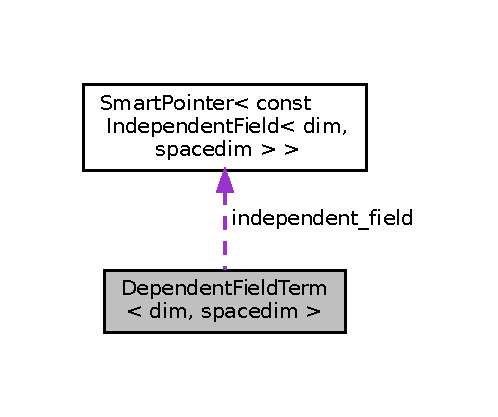
\includegraphics[width=220pt]{class_dependent_field_term__coll__graph}
\end{center}
\end{figure}
\subsection*{Public Member Functions}
\begin{DoxyCompactItemize}
\item 
\hyperlink{class_dependent_field_term_a149a09f602b0baadba9033d6a8da448c}{Dependent\+Field\+Term} (const double \hyperlink{class_dependent_field_term_a59a9183a32ac55fb728f3797b68a9f8f}{coefficient}, const \hyperlink{class_independent_field}{Independent\+Field}$<$ dim, spacedim $>$ \&\hyperlink{class_dependent_field_term_a89d1c3fea36e6fe105232097a321e095}{independent\+\_\+field}, const unsigned int \hyperlink{class_dependent_field_term_ac6f3ac40d4ee2c8b9f9bbdfa34079b74}{component}=0, const std\+::vector$<$ unsigned int $>$ \hyperlink{class_dependent_field_term_af09c5452c3e8e71e9ee99db304b90135}{derivatives}=std\+::vector$<$ unsigned int $>$())
\item 
double \hyperlink{class_dependent_field_term_a9c477ae87acdea43960f399ca2dd10b9}{first\+\_\+derivative} () const 
\item 
unsigned int \hyperlink{class_dependent_field_term_aa1c7aeb391135d4cafa1f208c15517ec}{n\+\_\+derivatives} () const 
\item 
bool \hyperlink{class_dependent_field_term_ab9934d7ad41e3a52073cc11293e7178b}{operator$<$} (const \hyperlink{class_dependent_field_term}{Dependent\+Field\+Term} \&dependent\+\_\+field\+\_\+2) const 
\end{DoxyCompactItemize}
\subsection*{Public Attributes}
\begin{DoxyCompactItemize}
\item 
const double \hyperlink{class_dependent_field_term_a59a9183a32ac55fb728f3797b68a9f8f}{coefficient}
\item 
const {\bf Smart\+Pointer}$<$ const \hyperlink{class_independent_field}{Independent\+Field}$<$ dim, spacedim $>$ $>$ \hyperlink{class_dependent_field_term_a89d1c3fea36e6fe105232097a321e095}{independent\+\_\+field}
\item 
const unsigned int \hyperlink{class_dependent_field_term_ac6f3ac40d4ee2c8b9f9bbdfa34079b74}{component}
\item 
const std\+::vector$<$ unsigned int $>$ \hyperlink{class_dependent_field_term_af09c5452c3e8e71e9ee99db304b90135}{derivatives}
\end{DoxyCompactItemize}


\subsection{Detailed Description}
\subsubsection*{template$<$unsigned int dim, unsigned int spacedim$>$\\*
class Dependent\+Field\+Term$<$ dim, spacedim $>$}

This class allows for the definition of a term of the form $a \dfrac{\partial^N f}{\partial x_{i_0} \hdots \partial x_{i_{N-1}}} $, where $a$ is a constant coefficient, and $f$ is a function of the spatial location $\boldsymbol{x}$. The function $f$ is derived $N$ times with respect to particular spatial coordinates, which is indicated by the notation $\dfrac{\partial^N f}{\partial x_{i_0} \hdots \partial x_{i_{N-1}}}$. It is noted that the $i_k$ in the latter expression refer to fixed numbers. I.\+e., $\dfrac{\partial^N f}{\partial x_{i_0} \hdots \partial x_{i_{N-1}}}$ is scalar valued, with examples being $\dfrac{\partial f}{\partial x_2}$ and $\dfrac{\partial^2 f}{\partial x_2 \partial x_1}$. \char`\"{}\+Zeroth\char`\"{} derivatives are also allowed by this class (i.\+e., terms of the form $a f$).

In particular, the function $f$ may either be a domain related independent field $u^\Omega_\epsilon$ or an interface related independent field $u^\Sigma_\eta$.


\begin{DoxyTemplParams}{Template Parameters}
{\em dim} & The dimension of the object on which the function $f$ lives\\
\hline
{\em spacedim} & The spatial dimension of the problem \\
\hline
\end{DoxyTemplParams}


\subsection{Constructor \& Destructor Documentation}
\index{Dependent\+Field\+Term@{Dependent\+Field\+Term}!Dependent\+Field\+Term@{Dependent\+Field\+Term}}
\index{Dependent\+Field\+Term@{Dependent\+Field\+Term}!Dependent\+Field\+Term@{Dependent\+Field\+Term}}
\subsubsection[{\texorpdfstring{Dependent\+Field\+Term(const double coefficient, const Independent\+Field$<$ dim, spacedim $>$ \&independent\+\_\+field, const unsigned int component=0, const std\+::vector$<$ unsigned int $>$ derivatives=std\+::vector$<$ unsigned int $>$())}{DependentFieldTerm(const double coefficient, const IndependentField< dim, spacedim > &independent_field, const unsigned int component=0, const std::vector< unsigned int > derivatives=std::vector< unsigned int >())}}]{\setlength{\rightskip}{0pt plus 5cm}template$<$unsigned int dim, unsigned int spacedim$>$ {\bf Dependent\+Field\+Term}$<$ dim, spacedim $>$\+::{\bf Dependent\+Field\+Term} (
\begin{DoxyParamCaption}
\item[{const double}]{coefficient, }
\item[{const {\bf Independent\+Field}$<$ dim, spacedim $>$ \&}]{independent\+\_\+field, }
\item[{const unsigned int}]{component = {\ttfamily 0}, }
\item[{const std\+::vector$<$ unsigned int $>$}]{derivatives = {\ttfamily std\+:\+:vector$<$~unsigned~int~$>$()}}
\end{DoxyParamCaption}
)}\hypertarget{class_dependent_field_term_a149a09f602b0baadba9033d6a8da448c}{}\label{class_dependent_field_term_a149a09f602b0baadba9033d6a8da448c}
The constructor of the class.


\begin{DoxyParams}[1]{Parameters}
\mbox{\tt in}  & {\em coefficient} & \hyperlink{class_dependent_field_term_a59a9183a32ac55fb728f3797b68a9f8f}{Dependent\+Field\+Term\+::coefficient} \\
\hline
\mbox{\tt in}  & {\em independent\+\_\+field} & \hyperlink{class_dependent_field_term_a89d1c3fea36e6fe105232097a321e095}{Dependent\+Field\+Term\+::independent\+\_\+field} \\
\hline
\mbox{\tt in}  & {\em component} & \hyperlink{class_dependent_field_term_ac6f3ac40d4ee2c8b9f9bbdfa34079b74}{Dependent\+Field\+Term\+::component} \\
\hline
\mbox{\tt in}  & {\em derivatives} & \hyperlink{class_dependent_field_term_af09c5452c3e8e71e9ee99db304b90135}{Dependent\+Field\+Term\+::derivatives} \\
\hline
\end{DoxyParams}


\subsection{Member Function Documentation}
\index{Dependent\+Field\+Term@{Dependent\+Field\+Term}!first\+\_\+derivative@{first\+\_\+derivative}}
\index{first\+\_\+derivative@{first\+\_\+derivative}!Dependent\+Field\+Term@{Dependent\+Field\+Term}}
\subsubsection[{\texorpdfstring{first\+\_\+derivative() const }{first_derivative() const }}]{\setlength{\rightskip}{0pt plus 5cm}template$<$unsigned int dim, unsigned int spacedim$>$ double {\bf Dependent\+Field\+Term}$<$ dim, spacedim $>$\+::first\+\_\+derivative (
\begin{DoxyParamCaption}
{}
\end{DoxyParamCaption}
) const}\hypertarget{class_dependent_field_term_a9c477ae87acdea43960f399ca2dd10b9}{}\label{class_dependent_field_term_a9c477ae87acdea43960f399ca2dd10b9}
\begin{DoxyReturn}{Returns}
\hyperlink{class_dependent_field_term_af09c5452c3e8e71e9ee99db304b90135}{Dependent\+Field\+Term\+::derivatives}\mbox{[}0\mbox{]} 
\end{DoxyReturn}
\index{Dependent\+Field\+Term@{Dependent\+Field\+Term}!n\+\_\+derivatives@{n\+\_\+derivatives}}
\index{n\+\_\+derivatives@{n\+\_\+derivatives}!Dependent\+Field\+Term@{Dependent\+Field\+Term}}
\subsubsection[{\texorpdfstring{n\+\_\+derivatives() const }{n_derivatives() const }}]{\setlength{\rightskip}{0pt plus 5cm}template$<$unsigned int dim, unsigned int spacedim$>$ unsigned int {\bf Dependent\+Field\+Term}$<$ dim, spacedim $>$\+::n\+\_\+derivatives (
\begin{DoxyParamCaption}
{}
\end{DoxyParamCaption}
) const}\hypertarget{class_dependent_field_term_aa1c7aeb391135d4cafa1f208c15517ec}{}\label{class_dependent_field_term_aa1c7aeb391135d4cafa1f208c15517ec}
\begin{DoxyReturn}{Returns}
The size of \hyperlink{class_dependent_field_term_af09c5452c3e8e71e9ee99db304b90135}{Dependent\+Field\+Term\+::derivatives} (i.\+e. $N$) 
\end{DoxyReturn}
\index{Dependent\+Field\+Term@{Dependent\+Field\+Term}!operator$<$@{operator$<$}}
\index{operator$<$@{operator$<$}!Dependent\+Field\+Term@{Dependent\+Field\+Term}}
\subsubsection[{\texorpdfstring{operator$<$(const Dependent\+Field\+Term \&dependent\+\_\+field\+\_\+2) const }{operator<(const DependentFieldTerm &dependent_field_2) const }}]{\setlength{\rightskip}{0pt plus 5cm}template$<$unsigned int dim, unsigned int spacedim$>$ bool {\bf Dependent\+Field\+Term}$<$ dim, spacedim $>$\+::operator$<$ (
\begin{DoxyParamCaption}
\item[{const {\bf Dependent\+Field\+Term}$<$ dim, spacedim $>$ \&}]{dependent\+\_\+field\+\_\+2}
\end{DoxyParamCaption}
) const}\hypertarget{class_dependent_field_term_ab9934d7ad41e3a52073cc11293e7178b}{}\label{class_dependent_field_term_ab9934d7ad41e3a52073cc11293e7178b}
A comparison operator, which allows to use \hyperlink{class_dependent_field_term}{Dependent\+Field\+Term} in {\ttfamily std\+::map} and {\ttfamily std\+::set}. The comparison operator is based on a lexicographic ordering according to the members \hyperlink{class_dependent_field_term_a89d1c3fea36e6fe105232097a321e095}{Dependent\+Field\+Term\+::independent\+\_\+field}, \hyperlink{class_dependent_field_term_ac6f3ac40d4ee2c8b9f9bbdfa34079b74}{Dependent\+Field\+Term\+::component}, \hyperlink{class_dependent_field_term_af09c5452c3e8e71e9ee99db304b90135}{Dependent\+Field\+Term\+::derivatives}. This means that the member \hyperlink{class_dependent_field_term_a59a9183a32ac55fb728f3797b68a9f8f}{Dependent\+Field\+Term\+::coefficient} does not factor into the comparison, which effectively means that two \hyperlink{class_dependent_field_term}{Dependent\+Field\+Term} objects are considered equal if they are associated with the same \hyperlink{class_dependent_field_term_a89d1c3fea36e6fe105232097a321e095}{Dependent\+Field\+Term\+::independent\+\_\+field}, \hyperlink{class_dependent_field_term_ac6f3ac40d4ee2c8b9f9bbdfa34079b74}{Dependent\+Field\+Term\+::component}, \hyperlink{class_dependent_field_term_af09c5452c3e8e71e9ee99db304b90135}{Dependent\+Field\+Term\+::derivatives} (the same \hyperlink{class_dependent_field_term_a89d1c3fea36e6fe105232097a321e095}{Dependent\+Field\+Term\+::independent\+\_\+field} here really means \char`\"{}exactly the same object\char`\"{}).


\begin{DoxyParams}[1]{Parameters}
\mbox{\tt in}  & {\em dependent\+\_\+field\+\_\+2} & The \hyperlink{class_dependent_field_term}{Dependent\+Field\+Term} to compare with\\
\hline
\end{DoxyParams}
\begin{DoxyReturn}{Returns}
Boolean indicating result of comparison 
\end{DoxyReturn}


\subsection{Member Data Documentation}
\index{Dependent\+Field\+Term@{Dependent\+Field\+Term}!coefficient@{coefficient}}
\index{coefficient@{coefficient}!Dependent\+Field\+Term@{Dependent\+Field\+Term}}
\subsubsection[{\texorpdfstring{coefficient}{coefficient}}]{\setlength{\rightskip}{0pt plus 5cm}template$<$unsigned int dim, unsigned int spacedim$>$ const double {\bf Dependent\+Field\+Term}$<$ dim, spacedim $>$\+::coefficient}\hypertarget{class_dependent_field_term_a59a9183a32ac55fb728f3797b68a9f8f}{}\label{class_dependent_field_term_a59a9183a32ac55fb728f3797b68a9f8f}
The coefficient $a$ \index{Dependent\+Field\+Term@{Dependent\+Field\+Term}!component@{component}}
\index{component@{component}!Dependent\+Field\+Term@{Dependent\+Field\+Term}}
\subsubsection[{\texorpdfstring{component}{component}}]{\setlength{\rightskip}{0pt plus 5cm}template$<$unsigned int dim, unsigned int spacedim$>$ const unsigned int {\bf Dependent\+Field\+Term}$<$ dim, spacedim $>$\+::component}\hypertarget{class_dependent_field_term_ac6f3ac40d4ee2c8b9f9bbdfa34079b74}{}\label{class_dependent_field_term_ac6f3ac40d4ee2c8b9f9bbdfa34079b74}
A component of the (possibly vector valued) \hyperlink{class_independent_field}{Independent\+Field} \hyperlink{class_dependent_field_term_a89d1c3fea36e6fe105232097a321e095}{Dependent\+Field\+Term\+::independent\+\_\+field}, which defines together with \hyperlink{class_dependent_field_term_a89d1c3fea36e6fe105232097a321e095}{Dependent\+Field\+Term\+::independent\+\_\+field} the independent field $f$. If \hyperlink{class_dependent_field_term_a89d1c3fea36e6fe105232097a321e095}{Dependent\+Field\+Term\+::independent\+\_\+field} is scalar valued, \hyperlink{class_dependent_field_term_ac6f3ac40d4ee2c8b9f9bbdfa34079b74}{Dependent\+Field\+Term\+::component} can only be zero. \index{Dependent\+Field\+Term@{Dependent\+Field\+Term}!derivatives@{derivatives}}
\index{derivatives@{derivatives}!Dependent\+Field\+Term@{Dependent\+Field\+Term}}
\subsubsection[{\texorpdfstring{derivatives}{derivatives}}]{\setlength{\rightskip}{0pt plus 5cm}template$<$unsigned int dim, unsigned int spacedim$>$ const std\+::vector$<$unsigned int$>$ {\bf Dependent\+Field\+Term}$<$ dim, spacedim $>$\+::derivatives}\hypertarget{class_dependent_field_term_af09c5452c3e8e71e9ee99db304b90135}{}\label{class_dependent_field_term_af09c5452c3e8e71e9ee99db304b90135}
A list of the spatial derivatives. The first element in the vector is $i_0$, the second element the derivative $i_1$, etc. The length of the vector is thus equal to the number of derivatives $N$; and in the special case that there are no derivatives, this vector will have the size zero. \index{Dependent\+Field\+Term@{Dependent\+Field\+Term}!independent\+\_\+field@{independent\+\_\+field}}
\index{independent\+\_\+field@{independent\+\_\+field}!Dependent\+Field\+Term@{Dependent\+Field\+Term}}
\subsubsection[{\texorpdfstring{independent\+\_\+field}{independent_field}}]{\setlength{\rightskip}{0pt plus 5cm}template$<$unsigned int dim, unsigned int spacedim$>$ const {\bf Smart\+Pointer}$<$const {\bf Independent\+Field}$<$dim, spacedim$>$ $>$ {\bf Dependent\+Field\+Term}$<$ dim, spacedim $>$\+::independent\+\_\+field}\hypertarget{class_dependent_field_term_a89d1c3fea36e6fe105232097a321e095}{}\label{class_dependent_field_term_a89d1c3fea36e6fe105232097a321e095}
An \hyperlink{class_independent_field}{Independent\+Field} object, which defines together with \hyperlink{class_dependent_field_term_ac6f3ac40d4ee2c8b9f9bbdfa34079b74}{Dependent\+Field\+Term\+::component}, the function $f$ 

The documentation for this class was generated from the following file\+:\begin{DoxyCompactItemize}
\item 
/home/sst/code/\+Galerkin\+Tools/\+Galerkin\+Tools/include/galerkin\+\_\+tools/\hyperlink{dependent__field_8h}{dependent\+\_\+field.\+h}\end{DoxyCompactItemize}

\hypertarget{class_dirichlet_constraint}{}\doxysection{Dirichlet\+Constraint$<$ spacedim $>$ Class Template Reference}
\label{class_dirichlet_constraint}\index{DirichletConstraint$<$ spacedim $>$@{DirichletConstraint$<$ spacedim $>$}}


{\ttfamily \#include $<$dirichlet\+\_\+constraint.\+h$>$}



Inheritance diagram for Dirichlet\+Constraint$<$ spacedim $>$\+:\nopagebreak
\begin{figure}[H]
\begin{center}
\leavevmode
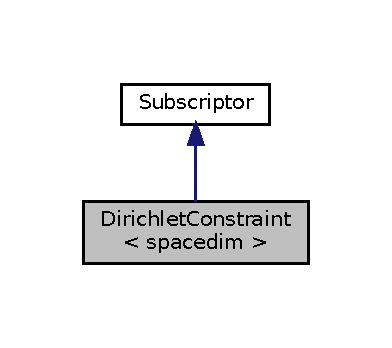
\includegraphics[width=188pt]{class_dirichlet_constraint__inherit__graph}
\end{center}
\end{figure}


Collaboration diagram for Dirichlet\+Constraint$<$ spacedim $>$\+:\nopagebreak
\begin{figure}[H]
\begin{center}
\leavevmode
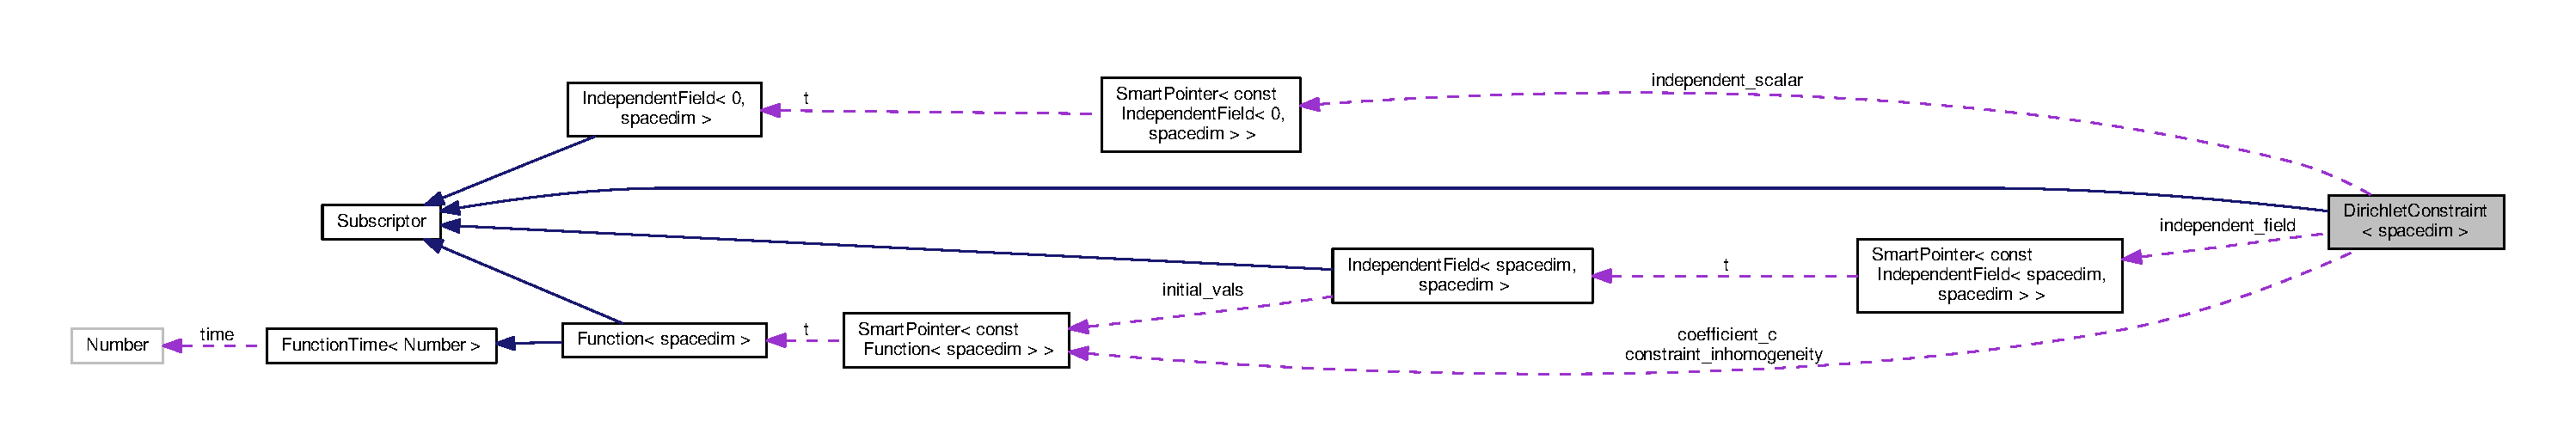
\includegraphics[width=350pt]{class_dirichlet_constraint__coll__graph}
\end{center}
\end{figure}
\doxysubsection*{Public Member Functions}
\begin{DoxyCompactItemize}
\item 
\mbox{\hyperlink{class_dirichlet_constraint_a14e75a7f8bcc8a18daa04a5c1164fe87}{Dirichlet\+Constraint}} (const \mbox{\hyperlink{class_independent_field}{Independent\+Field}}$<$ spacedim, spacedim $>$ \&\mbox{\hyperlink{class_dirichlet_constraint_abbd7945a973ed93d1d773307393ffde3}{independent\+\_\+field}}, const unsigned int \mbox{\hyperlink{class_dirichlet_constraint_a7e3c4d0e0906af1c81b88e05e41bdafc}{component}}, const \mbox{\hyperlink{triangulation__system_8h_a44f3c00e36c1d6e3c389ae693c09b435}{Interface\+Side}} \mbox{\hyperlink{class_dirichlet_constraint_ae049d107664d3bf23d287ec77545b6f3}{side}}, const std\+::set$<$ \textbf{ types\+::material\+\_\+id} $>$ \mbox{\hyperlink{class_dirichlet_constraint_a258b6ff11b206f966bb03943bb11f469}{domain\+\_\+of\+\_\+constraint}}, const \textbf{ Function}$<$ spacedim $>$ $\ast$const \mbox{\hyperlink{class_dirichlet_constraint_af22d2bca23999bdb4f2b67e8982d29c5}{constraint\+\_\+inhomogeneity}}=nullptr, const \mbox{\hyperlink{class_independent_field}{Independent\+Field}}$<$ 0, spacedim $>$ $\ast$\mbox{\hyperlink{class_dirichlet_constraint_a8793f0d41a9c6e88638d7cf5d52a6fdd}{independent\+\_\+scalar}}=nullptr, const \textbf{ Function}$<$ spacedim $>$ $\ast$const \mbox{\hyperlink{class_dirichlet_constraint_adea2dc6126a633b297eb7dfce832b9ef}{coefficient\+\_\+c}}=nullptr)
\item 
virtual \mbox{\hyperlink{class_dirichlet_constraint_ac6b6b7caf4694000486abff377fd1440}{$\sim$\+Dirichlet\+Constraint}} ()
\item 
void \mbox{\hyperlink{class_dirichlet_constraint_abdfdde6ef50639152e2a82d54b130042}{set\+\_\+constraint\+\_\+is\+\_\+active}} (const bool \mbox{\hyperlink{class_dirichlet_constraint_a1ae0b53768be76747f31b5bc584d9ed6}{constraint\+\_\+is\+\_\+active}})
\item 
bool \mbox{\hyperlink{class_dirichlet_constraint_ad1741529befff8fca4af6ee82224abb3}{get\+\_\+constraint\+\_\+is\+\_\+active}} () const
\item 
void \mbox{\hyperlink{class_dirichlet_constraint_ab8c509170d5d36f778415b88bceee99d}{set\+\_\+time}} (const double time) const
\end{DoxyCompactItemize}
\doxysubsection*{Public Attributes}
\begin{DoxyCompactItemize}
\item 
const std\+::set$<$ \textbf{ types\+::material\+\_\+id} $>$ \mbox{\hyperlink{class_dirichlet_constraint_a258b6ff11b206f966bb03943bb11f469}{domain\+\_\+of\+\_\+constraint}}
\item 
const \textbf{ Smart\+Pointer}$<$ const \mbox{\hyperlink{class_independent_field}{Independent\+Field}}$<$ spacedim, spacedim $>$ $>$ \mbox{\hyperlink{class_dirichlet_constraint_abbd7945a973ed93d1d773307393ffde3}{independent\+\_\+field}}
\item 
const unsigned int \mbox{\hyperlink{class_dirichlet_constraint_a7e3c4d0e0906af1c81b88e05e41bdafc}{component}}
\item 
const \mbox{\hyperlink{triangulation__system_8h_a44f3c00e36c1d6e3c389ae693c09b435}{Interface\+Side}} \mbox{\hyperlink{class_dirichlet_constraint_ae049d107664d3bf23d287ec77545b6f3}{side}}
\item 
const \textbf{ Smart\+Pointer}$<$ const \textbf{ Function}$<$ spacedim $>$ $>$ \mbox{\hyperlink{class_dirichlet_constraint_af22d2bca23999bdb4f2b67e8982d29c5}{constraint\+\_\+inhomogeneity}}
\item 
const \textbf{ Smart\+Pointer}$<$ const \mbox{\hyperlink{class_independent_field}{Independent\+Field}}$<$ 0, spacedim $>$ $>$ \mbox{\hyperlink{class_dirichlet_constraint_a8793f0d41a9c6e88638d7cf5d52a6fdd}{independent\+\_\+scalar}}
\item 
const \textbf{ Smart\+Pointer}$<$ const \textbf{ Function}$<$ spacedim $>$ $>$ \mbox{\hyperlink{class_dirichlet_constraint_adea2dc6126a633b297eb7dfce832b9ef}{coefficient\+\_\+c}}
\end{DoxyCompactItemize}
\doxysubsection*{Private Attributes}
\begin{DoxyCompactItemize}
\item 
bool \mbox{\hyperlink{class_dirichlet_constraint_a1ae0b53768be76747f31b5bc584d9ed6}{constraint\+\_\+is\+\_\+active}} = true
\end{DoxyCompactItemize}
\doxysubsection*{Additional Inherited Members}


\doxysubsection{Detailed Description}
\subsubsection*{template$<$unsigned int spacedim$>$\newline
class Dirichlet\+Constraint$<$ spacedim $>$}

Class defining a Dirichlet type interface condition for a domain related independent variable $u^\Omega_\epsilon$.

The Dirichlet type condition has the form $ \left(u^\Omega_\epsilon\right)^+ = b^\Omega_\epsilon + c^\Omega_\epsilon C_\iota$ or $ \left(u^\Omega_\epsilon\right)^- = b^\Omega_\epsilon + c^\Omega_\epsilon C_\iota$, where $b^\Omega_\epsilon$ and $c^\Omega_\epsilon$ are prescribed functions, which may depend on the spatial position on the interface; and + or -\/ indicates the side of the interface on which the Dirichlet type condition applies; and $C_\iota$ is a independent scalar (including this term allows to implement b.\+c.\+s of the form $u^\Omega_\epsilon = \mathrm{const.}$)

\begin{DoxyRefDesc}{Todo}
\item[\mbox{\hyperlink{todo__todo000008}{Todo}}]It would be desirable to also allow for Dirichlet type conditions on interface related fields (these conditions would then be imposed on codim 2 objects). This is not implemented yet.\end{DoxyRefDesc}


The \mbox{\hyperlink{class_dirichlet_constraint}{Dirichlet\+Constraint}} class inherits from \textbf{ Subscriptor} in order to be able to check that \mbox{\hyperlink{class_dirichlet_constraint}{Dirichlet\+Constraint}} objects are only destroyed when they are not needed anymore by other objects.


\begin{DoxyTemplParams}{Template Parameters}
{\em spacedim} & Spatial dimension of the problem \\
\hline
\end{DoxyTemplParams}


\doxysubsection{Constructor \& Destructor Documentation}
\mbox{\Hypertarget{class_dirichlet_constraint_a14e75a7f8bcc8a18daa04a5c1164fe87}\label{class_dirichlet_constraint_a14e75a7f8bcc8a18daa04a5c1164fe87}} 
\index{DirichletConstraint$<$ spacedim $>$@{DirichletConstraint$<$ spacedim $>$}!DirichletConstraint@{DirichletConstraint}}
\index{DirichletConstraint@{DirichletConstraint}!DirichletConstraint$<$ spacedim $>$@{DirichletConstraint$<$ spacedim $>$}}
\doxysubsubsection{\texorpdfstring{DirichletConstraint()}{DirichletConstraint()}}
{\footnotesize\ttfamily template$<$unsigned int spacedim$>$ \\
\mbox{\hyperlink{class_dirichlet_constraint}{Dirichlet\+Constraint}}$<$ spacedim $>$\+::\mbox{\hyperlink{class_dirichlet_constraint}{Dirichlet\+Constraint}} (\begin{DoxyParamCaption}\item[{const \mbox{\hyperlink{class_independent_field}{Independent\+Field}}$<$ spacedim, spacedim $>$ \&}]{independent\+\_\+field,  }\item[{const unsigned int}]{component,  }\item[{const \mbox{\hyperlink{triangulation__system_8h_a44f3c00e36c1d6e3c389ae693c09b435}{Interface\+Side}}}]{side,  }\item[{const std\+::set$<$ \textbf{ types\+::material\+\_\+id} $>$}]{domain\+\_\+of\+\_\+constraint,  }\item[{const \textbf{ Function}$<$ spacedim $>$ $\ast$const}]{constraint\+\_\+inhomogeneity = {\ttfamily nullptr},  }\item[{const \mbox{\hyperlink{class_independent_field}{Independent\+Field}}$<$ 0, spacedim $>$ $\ast$}]{independent\+\_\+scalar = {\ttfamily nullptr},  }\item[{const \textbf{ Function}$<$ spacedim $>$ $\ast$const}]{coefficient\+\_\+c = {\ttfamily nullptr} }\end{DoxyParamCaption})}

The constructor of the class


\begin{DoxyParams}[1]{Parameters}
\mbox{\texttt{ in}}  & {\em independent\+\_\+field} & \mbox{\hyperlink{class_dirichlet_constraint_abbd7945a973ed93d1d773307393ffde3}{Dirichlet\+Constraint\+::independent\+\_\+field}}\\
\hline
\mbox{\texttt{ in}}  & {\em component} & \mbox{\hyperlink{class_dirichlet_constraint_a7e3c4d0e0906af1c81b88e05e41bdafc}{Dirichlet\+Constraint\+::component}}\\
\hline
\mbox{\texttt{ in}}  & {\em side} & \mbox{\hyperlink{class_dirichlet_constraint_ae049d107664d3bf23d287ec77545b6f3}{Dirichlet\+Constraint\+::side}}\\
\hline
\mbox{\texttt{ in}}  & {\em domain\+\_\+of\+\_\+constraint} & \mbox{\hyperlink{class_dirichlet_constraint_a258b6ff11b206f966bb03943bb11f469}{Dirichlet\+Constraint\+::domain\+\_\+of\+\_\+constraint}}\\
\hline
\mbox{\texttt{ in}}  & {\em constraint\+\_\+inhomogeneity} & \mbox{\hyperlink{class_dirichlet_constraint_af22d2bca23999bdb4f2b67e8982d29c5}{Dirichlet\+Constraint\+::constraint\+\_\+inhomogeneity}}\\
\hline
\mbox{\texttt{ in}}  & {\em independent\+\_\+scalar} & \mbox{\hyperlink{class_dirichlet_constraint_a8793f0d41a9c6e88638d7cf5d52a6fdd}{Dirichlet\+Constraint\+::independent\+\_\+scalar}}\\
\hline
\mbox{\texttt{ in}}  & {\em coefficient\+\_\+c} & \mbox{\hyperlink{class_dirichlet_constraint_adea2dc6126a633b297eb7dfce832b9ef}{Dirichlet\+Constraint\+::coefficient\+\_\+c}} \\
\hline
\end{DoxyParams}
\mbox{\Hypertarget{class_dirichlet_constraint_ac6b6b7caf4694000486abff377fd1440}\label{class_dirichlet_constraint_ac6b6b7caf4694000486abff377fd1440}} 
\index{DirichletConstraint$<$ spacedim $>$@{DirichletConstraint$<$ spacedim $>$}!````~DirichletConstraint@{$\sim$DirichletConstraint}}
\index{````~DirichletConstraint@{$\sim$DirichletConstraint}!DirichletConstraint$<$ spacedim $>$@{DirichletConstraint$<$ spacedim $>$}}
\doxysubsubsection{\texorpdfstring{$\sim$DirichletConstraint()}{~DirichletConstraint()}}
{\footnotesize\ttfamily template$<$unsigned int spacedim$>$ \\
virtual \mbox{\hyperlink{class_dirichlet_constraint}{Dirichlet\+Constraint}}$<$ spacedim $>$\+::$\sim$\mbox{\hyperlink{class_dirichlet_constraint}{Dirichlet\+Constraint}} (\begin{DoxyParamCaption}{ }\end{DoxyParamCaption})\hspace{0.3cm}{\ttfamily [virtual]}}

The destructor of \mbox{\hyperlink{class_dirichlet_constraint}{Dirichlet\+Constraint}} essentially checks before destruction that the \mbox{\hyperlink{class_dirichlet_constraint}{Dirichlet\+Constraint}} object is not used by other objects. If this is the case, the program will be aborted. 

\doxysubsection{Member Function Documentation}
\mbox{\Hypertarget{class_dirichlet_constraint_ad1741529befff8fca4af6ee82224abb3}\label{class_dirichlet_constraint_ad1741529befff8fca4af6ee82224abb3}} 
\index{DirichletConstraint$<$ spacedim $>$@{DirichletConstraint$<$ spacedim $>$}!get\_constraint\_is\_active@{get\_constraint\_is\_active}}
\index{get\_constraint\_is\_active@{get\_constraint\_is\_active}!DirichletConstraint$<$ spacedim $>$@{DirichletConstraint$<$ spacedim $>$}}
\doxysubsubsection{\texorpdfstring{get\_constraint\_is\_active()}{get\_constraint\_is\_active()}}
{\footnotesize\ttfamily template$<$unsigned int spacedim$>$ \\
bool \mbox{\hyperlink{class_dirichlet_constraint}{Dirichlet\+Constraint}}$<$ spacedim $>$\+::get\+\_\+constraint\+\_\+is\+\_\+active (\begin{DoxyParamCaption}{ }\end{DoxyParamCaption}) const}

Return \mbox{\hyperlink{class_dirichlet_constraint_a1ae0b53768be76747f31b5bc584d9ed6}{Dirichlet\+Constraint\+::constraint\+\_\+is\+\_\+active}} \mbox{\Hypertarget{class_dirichlet_constraint_abdfdde6ef50639152e2a82d54b130042}\label{class_dirichlet_constraint_abdfdde6ef50639152e2a82d54b130042}} 
\index{DirichletConstraint$<$ spacedim $>$@{DirichletConstraint$<$ spacedim $>$}!set\_constraint\_is\_active@{set\_constraint\_is\_active}}
\index{set\_constraint\_is\_active@{set\_constraint\_is\_active}!DirichletConstraint$<$ spacedim $>$@{DirichletConstraint$<$ spacedim $>$}}
\doxysubsubsection{\texorpdfstring{set\_constraint\_is\_active()}{set\_constraint\_is\_active()}}
{\footnotesize\ttfamily template$<$unsigned int spacedim$>$ \\
void \mbox{\hyperlink{class_dirichlet_constraint}{Dirichlet\+Constraint}}$<$ spacedim $>$\+::set\+\_\+constraint\+\_\+is\+\_\+active (\begin{DoxyParamCaption}\item[{const bool}]{constraint\+\_\+is\+\_\+active }\end{DoxyParamCaption})}

Sets \mbox{\hyperlink{class_dirichlet_constraint_a1ae0b53768be76747f31b5bc584d9ed6}{Dirichlet\+Constraint\+::constraint\+\_\+is\+\_\+active}}


\begin{DoxyParams}[1]{Parameters}
\mbox{\texttt{ in}}  & {\em constraint\+\_\+is\+\_\+active} & Value to be assigned to \mbox{\hyperlink{class_dirichlet_constraint_a1ae0b53768be76747f31b5bc584d9ed6}{Dirichlet\+Constraint\+::constraint\+\_\+is\+\_\+active}} \\
\hline
\end{DoxyParams}
\mbox{\Hypertarget{class_dirichlet_constraint_ab8c509170d5d36f778415b88bceee99d}\label{class_dirichlet_constraint_ab8c509170d5d36f778415b88bceee99d}} 
\index{DirichletConstraint$<$ spacedim $>$@{DirichletConstraint$<$ spacedim $>$}!set\_time@{set\_time}}
\index{set\_time@{set\_time}!DirichletConstraint$<$ spacedim $>$@{DirichletConstraint$<$ spacedim $>$}}
\doxysubsubsection{\texorpdfstring{set\_time()}{set\_time()}}
{\footnotesize\ttfamily template$<$unsigned int spacedim$>$ \\
void \mbox{\hyperlink{class_dirichlet_constraint}{Dirichlet\+Constraint}}$<$ spacedim $>$\+::set\+\_\+time (\begin{DoxyParamCaption}\item[{const double}]{time }\end{DoxyParamCaption}) const}

Set the time at which the constraint is evaluated


\begin{DoxyParams}[1]{Parameters}
\mbox{\texttt{ in}}  & {\em time} & The time at which the constraint is evaluated \\
\hline
\end{DoxyParams}


\doxysubsection{Member Data Documentation}
\mbox{\Hypertarget{class_dirichlet_constraint_adea2dc6126a633b297eb7dfce832b9ef}\label{class_dirichlet_constraint_adea2dc6126a633b297eb7dfce832b9ef}} 
\index{DirichletConstraint$<$ spacedim $>$@{DirichletConstraint$<$ spacedim $>$}!coefficient\_c@{coefficient\_c}}
\index{coefficient\_c@{coefficient\_c}!DirichletConstraint$<$ spacedim $>$@{DirichletConstraint$<$ spacedim $>$}}
\doxysubsubsection{\texorpdfstring{coefficient\_c}{coefficient\_c}}
{\footnotesize\ttfamily template$<$unsigned int spacedim$>$ \\
const \textbf{ Smart\+Pointer}$<$const \textbf{ Function}$<$spacedim$>$ $>$ \mbox{\hyperlink{class_dirichlet_constraint}{Dirichlet\+Constraint}}$<$ spacedim $>$\+::coefficient\+\_\+c}

A \textbf{ Function} (or, rather, an instance of a derived class) specifying $c^\Omega_\epsilon$ in dependence on the spatial position. The \textbf{ Function} must have a single component and implement the method \textbf{ Function\+::value()}. If a {\ttfamily nullptr} is stored here, the function will be taken as uniformly one. \mbox{\Hypertarget{class_dirichlet_constraint_a7e3c4d0e0906af1c81b88e05e41bdafc}\label{class_dirichlet_constraint_a7e3c4d0e0906af1c81b88e05e41bdafc}} 
\index{DirichletConstraint$<$ spacedim $>$@{DirichletConstraint$<$ spacedim $>$}!component@{component}}
\index{component@{component}!DirichletConstraint$<$ spacedim $>$@{DirichletConstraint$<$ spacedim $>$}}
\doxysubsubsection{\texorpdfstring{component}{component}}
{\footnotesize\ttfamily template$<$unsigned int spacedim$>$ \\
const unsigned int \mbox{\hyperlink{class_dirichlet_constraint}{Dirichlet\+Constraint}}$<$ spacedim $>$\+::component}

component of \mbox{\hyperlink{class_independent_field}{Independent\+Field}} object to be constrained (defines together with \mbox{\hyperlink{class_dirichlet_constraint_abbd7945a973ed93d1d773307393ffde3}{Dirichlet\+Constraint\+::independent\+\_\+field}} $u^\Omega_\epsilon$) \mbox{\Hypertarget{class_dirichlet_constraint_af22d2bca23999bdb4f2b67e8982d29c5}\label{class_dirichlet_constraint_af22d2bca23999bdb4f2b67e8982d29c5}} 
\index{DirichletConstraint$<$ spacedim $>$@{DirichletConstraint$<$ spacedim $>$}!constraint\_inhomogeneity@{constraint\_inhomogeneity}}
\index{constraint\_inhomogeneity@{constraint\_inhomogeneity}!DirichletConstraint$<$ spacedim $>$@{DirichletConstraint$<$ spacedim $>$}}
\doxysubsubsection{\texorpdfstring{constraint\_inhomogeneity}{constraint\_inhomogeneity}}
{\footnotesize\ttfamily template$<$unsigned int spacedim$>$ \\
const \textbf{ Smart\+Pointer}$<$const \textbf{ Function}$<$spacedim$>$ $>$ \mbox{\hyperlink{class_dirichlet_constraint}{Dirichlet\+Constraint}}$<$ spacedim $>$\+::constraint\+\_\+inhomogeneity}

A \textbf{ Function} (or, rather, an instance of a derived class) specifying the constraint inhomogeneity $b^\Omega_\epsilon$ in dependence on the spatial position. The \textbf{ Function} must have a single component and implement the method \textbf{ Function\+::value()}. If a {\ttfamily nullptr} is stored here, the constraint will be assumed homogeneous. \mbox{\Hypertarget{class_dirichlet_constraint_a1ae0b53768be76747f31b5bc584d9ed6}\label{class_dirichlet_constraint_a1ae0b53768be76747f31b5bc584d9ed6}} 
\index{DirichletConstraint$<$ spacedim $>$@{DirichletConstraint$<$ spacedim $>$}!constraint\_is\_active@{constraint\_is\_active}}
\index{constraint\_is\_active@{constraint\_is\_active}!DirichletConstraint$<$ spacedim $>$@{DirichletConstraint$<$ spacedim $>$}}
\doxysubsubsection{\texorpdfstring{constraint\_is\_active}{constraint\_is\_active}}
{\footnotesize\ttfamily template$<$unsigned int spacedim$>$ \\
bool \mbox{\hyperlink{class_dirichlet_constraint}{Dirichlet\+Constraint}}$<$ spacedim $>$\+::constraint\+\_\+is\+\_\+active = true\hspace{0.3cm}{\ttfamily [private]}}

Bool indicating whether constraint is currently active \mbox{\Hypertarget{class_dirichlet_constraint_a258b6ff11b206f966bb03943bb11f469}\label{class_dirichlet_constraint_a258b6ff11b206f966bb03943bb11f469}} 
\index{DirichletConstraint$<$ spacedim $>$@{DirichletConstraint$<$ spacedim $>$}!domain\_of\_constraint@{domain\_of\_constraint}}
\index{domain\_of\_constraint@{domain\_of\_constraint}!DirichletConstraint$<$ spacedim $>$@{DirichletConstraint$<$ spacedim $>$}}
\doxysubsubsection{\texorpdfstring{domain\_of\_constraint}{domain\_of\_constraint}}
{\footnotesize\ttfamily template$<$unsigned int spacedim$>$ \\
const std\+::set$<$\textbf{ types\+::material\+\_\+id}$>$ \mbox{\hyperlink{class_dirichlet_constraint}{Dirichlet\+Constraint}}$<$ spacedim $>$\+::domain\+\_\+of\+\_\+constraint}

\textbf{ types\+::material\+\_\+id}s determining the portions of the interface on which the constraint is applied \mbox{\Hypertarget{class_dirichlet_constraint_abbd7945a973ed93d1d773307393ffde3}\label{class_dirichlet_constraint_abbd7945a973ed93d1d773307393ffde3}} 
\index{DirichletConstraint$<$ spacedim $>$@{DirichletConstraint$<$ spacedim $>$}!independent\_field@{independent\_field}}
\index{independent\_field@{independent\_field}!DirichletConstraint$<$ spacedim $>$@{DirichletConstraint$<$ spacedim $>$}}
\doxysubsubsection{\texorpdfstring{independent\_field}{independent\_field}}
{\footnotesize\ttfamily template$<$unsigned int spacedim$>$ \\
const \textbf{ Smart\+Pointer}$<$const \mbox{\hyperlink{class_independent_field}{Independent\+Field}}$<$spacedim, spacedim$>$ $>$ \mbox{\hyperlink{class_dirichlet_constraint}{Dirichlet\+Constraint}}$<$ spacedim $>$\+::independent\+\_\+field}

\mbox{\hyperlink{class_independent_field}{Independent\+Field}} object to be constrained (defines together with \mbox{\hyperlink{class_dirichlet_constraint_a7e3c4d0e0906af1c81b88e05e41bdafc}{Dirichlet\+Constraint\+::component}} $u^\Omega_\epsilon$) \mbox{\Hypertarget{class_dirichlet_constraint_a8793f0d41a9c6e88638d7cf5d52a6fdd}\label{class_dirichlet_constraint_a8793f0d41a9c6e88638d7cf5d52a6fdd}} 
\index{DirichletConstraint$<$ spacedim $>$@{DirichletConstraint$<$ spacedim $>$}!independent\_scalar@{independent\_scalar}}
\index{independent\_scalar@{independent\_scalar}!DirichletConstraint$<$ spacedim $>$@{DirichletConstraint$<$ spacedim $>$}}
\doxysubsubsection{\texorpdfstring{independent\_scalar}{independent\_scalar}}
{\footnotesize\ttfamily template$<$unsigned int spacedim$>$ \\
const \textbf{ Smart\+Pointer}$<$const \mbox{\hyperlink{class_independent_field}{Independent\+Field}}$<$0, spacedim$>$ $>$ \mbox{\hyperlink{class_dirichlet_constraint}{Dirichlet\+Constraint}}$<$ spacedim $>$\+::independent\+\_\+scalar}

$C_\iota$ \mbox{\Hypertarget{class_dirichlet_constraint_ae049d107664d3bf23d287ec77545b6f3}\label{class_dirichlet_constraint_ae049d107664d3bf23d287ec77545b6f3}} 
\index{DirichletConstraint$<$ spacedim $>$@{DirichletConstraint$<$ spacedim $>$}!side@{side}}
\index{side@{side}!DirichletConstraint$<$ spacedim $>$@{DirichletConstraint$<$ spacedim $>$}}
\doxysubsubsection{\texorpdfstring{side}{side}}
{\footnotesize\ttfamily template$<$unsigned int spacedim$>$ \\
const \mbox{\hyperlink{triangulation__system_8h_a44f3c00e36c1d6e3c389ae693c09b435}{Interface\+Side}} \mbox{\hyperlink{class_dirichlet_constraint}{Dirichlet\+Constraint}}$<$ spacedim $>$\+::side}

Side of the interface (\mbox{\hyperlink{triangulation__system_8h_a44f3c00e36c1d6e3c389ae693c09b435}{Interface\+Side}}\+:\+:{\ttfamily plus} or \mbox{\hyperlink{triangulation__system_8h_a44f3c00e36c1d6e3c389ae693c09b435}{Interface\+Side}}\+:\+:{\ttfamily minus}) on which constraint applies; this information is relevant if the independent field is discontinuous across the interface. 

The documentation for this class was generated from the following file\+:\begin{DoxyCompactItemize}
\item 
/home/sst/code/\+Galerkin\+Tools/\+Galerkin\+Tools/include/galerkin\+\_\+tools/\mbox{\hyperlink{dirichlet__constraint_8h}{dirichlet\+\_\+constraint.\+h}}\end{DoxyCompactItemize}

\hypertarget{class_do_f_handler_system}{}\section{Do\+F\+Handler\+System$<$ spacedim $>$ Class Template Reference}
\label{class_do_f_handler_system}\index{Do\+F\+Handler\+System$<$ spacedim $>$@{Do\+F\+Handler\+System$<$ spacedim $>$}}


{\ttfamily \#include $<$dof\+\_\+handler\+\_\+system.\+h$>$}



Collaboration diagram for Do\+F\+Handler\+System$<$ spacedim $>$\+:\nopagebreak
\begin{figure}[H]
\begin{center}
\leavevmode
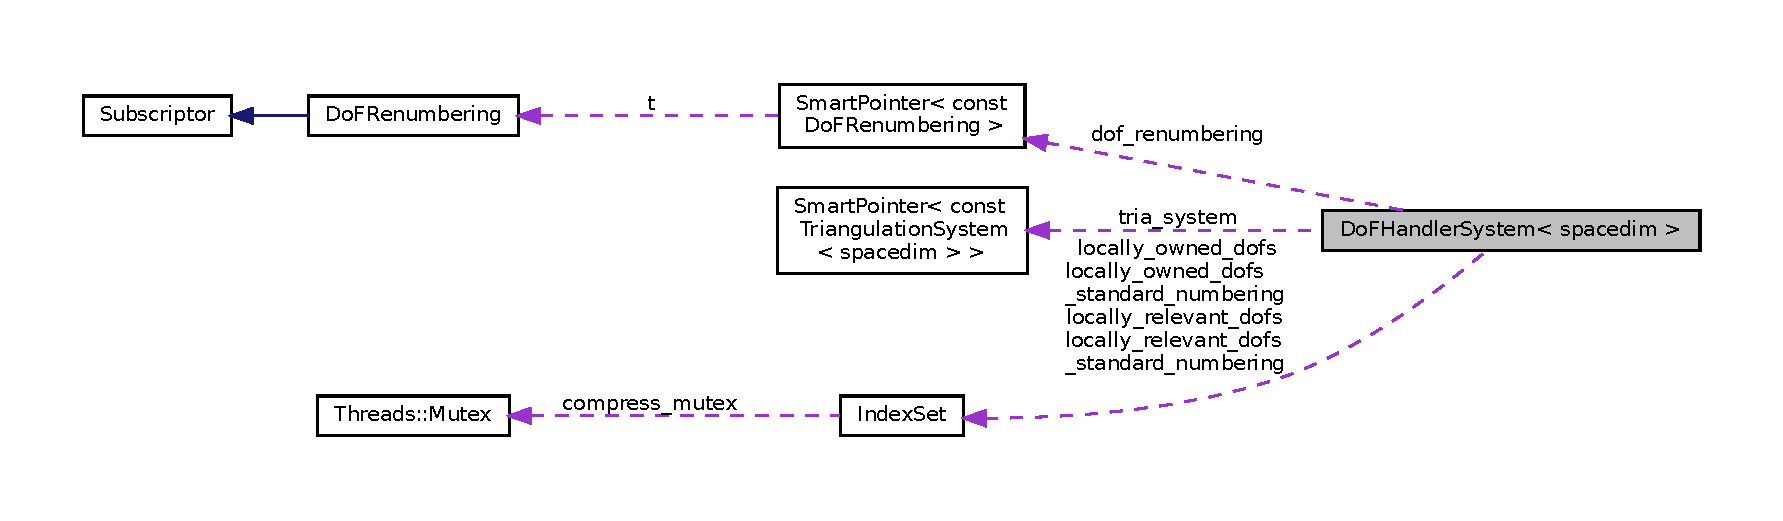
\includegraphics[width=350pt]{class_do_f_handler_system__coll__graph}
\end{center}
\end{figure}
\subsection*{Public Types}
\begin{DoxyCompactItemize}
\item 
typedef {\bf Tria\+Iterator}$<$ {\bf Cell\+Accessor}$<$ spacedim-\/1, spacedim $>$ $>$ \hyperlink{class_do_f_handler_system_a64bfb9dab5f61c2583896a7d086cb1f2}{Interface\+Cell}
\item 
typedef {\bf hp\+::\+Do\+F\+Handler}$<$ spacedim-\/1, spacedim $>$\+::{\bf cell\+\_\+iterator} \hyperlink{class_do_f_handler_system_a82e65f8c260f076489bd92615221a1d0}{Interface\+Cell\+DoF}
\item 
typedef {\bf Tria\+Iterator}$<$ {\bf Cell\+Accessor}$<$ spacedim, spacedim $>$ $>$ \hyperlink{class_do_f_handler_system_a84df955a5d8da7e1439a10f2a64811c0}{Domain\+Cell}
\item 
typedef {\bf hp\+::\+Do\+F\+Handler}$<$ spacedim, spacedim $>$\+::{\bf cell\+\_\+iterator} \hyperlink{class_do_f_handler_system_a01c54960bba8faa935d32f2d3d2fe914}{Domain\+Cell\+DoF}
\end{DoxyCompactItemize}
\subsection*{Public Member Functions}
\begin{DoxyCompactItemize}
\item 
\hyperlink{class_do_f_handler_system_acb31af36eec0abac1d6e764e3d08c7fe}{Do\+F\+Handler\+System} (const \hyperlink{class_triangulation_system}{Triangulation\+System}$<$ spacedim $>$ \&\hyperlink{class_do_f_handler_system_a06d93193cb47591db138cd8f41953796}{tria\+\_\+system})
\item 
\hyperlink{class_do_f_handler_system_a5a2f0389f4f4216b9841d9c518cb107e}{$\sim$\+Do\+F\+Handler\+System} ()
\item 
void \hyperlink{class_do_f_handler_system_ac6e0950ae9d140b0a9185bcfffe167d6}{distribute\+\_\+dofs} (const {\bf hp\+::\+F\+E\+Collection}$<$ spacedim, spacedim $>$ \&fe\+\_\+collection\+\_\+domain, const {\bf hp\+::\+F\+E\+Collection}$<$ spacedim-\/1, spacedim $>$ \&fe\+\_\+collection\+\_\+interface, const unsigned int n\+\_\+additional\+\_\+dofs=0)
\item 
void \hyperlink{class_do_f_handler_system_a1cbcc00826aca94736d3aebef157da72}{set\+\_\+fe} (const {\bf hp\+::\+F\+E\+Collection}$<$ spacedim, spacedim $>$ \&fe\+\_\+collection\+\_\+domain, const {\bf hp\+::\+F\+E\+Collection}$<$ spacedim-\/1, spacedim $>$ \&fe\+\_\+collection\+\_\+interface)
\item 
std\+::vector$<$ \hyperlink{class_interface_cell_domain_cells_do_f}{Interface\+Cell\+Domain\+Cells\+DoF}$<$ spacedim $>$ $>$\+::iterator \hyperlink{class_do_f_handler_system_a88d93ac03defd1b296238de4eb122841}{interface\+\_\+begin\+\_\+active} ()
\item 
std\+::vector$<$ \hyperlink{class_interface_cell_domain_cells_do_f}{Interface\+Cell\+Domain\+Cells\+DoF}$<$ spacedim $>$ $>$\+::iterator \hyperlink{class_do_f_handler_system_aecbc22a86943c1bc921a13ec7e2333f2}{interface\+\_\+end\+\_\+active} ()
\item 
const std\+::vector$<$ \hyperlink{class_interface_cell_domain_cells_do_f}{Interface\+Cell\+Domain\+Cells\+DoF}$<$ spacedim $>$ $>$ \& \hyperlink{class_do_f_handler_system_ae22105dc8db1090f12be9ecaed384228}{interface\+\_\+active\+\_\+iterators} () const 
\item 
\hyperlink{class_domain_cell_do_f_iterator}{Domain\+Cell\+Do\+F\+Iterator}$<$ spacedim $>$ \hyperlink{class_do_f_handler_system_aeee77ce076a84afdae132910c72de3b4}{domain\+\_\+begin\+\_\+active} () const 
\item 
\hyperlink{class_domain_cell_do_f_iterator}{Domain\+Cell\+Do\+F\+Iterator}$<$ spacedim $>$ \hyperlink{class_do_f_handler_system_afb624d9bed38a49be5ebbf16dd2abcd5}{domain\+\_\+end\+\_\+active} () const 
\item 
{\bf Iterator\+Range}$<$ \hyperlink{class_domain_cell_do_f_iterator}{Domain\+Cell\+Do\+F\+Iterator}$<$ spacedim $>$ $>$ \hyperlink{class_do_f_handler_system_a01759f9734ca7e762685d7c85fc30cad}{domain\+\_\+active\+\_\+iterators} () const 
\item 
unsigned int \hyperlink{class_do_f_handler_system_a69aca46be1a419d4ae3b66d57bed8b8e}{n\+\_\+dofs\+\_\+domain} () const 
\item 
unsigned int \hyperlink{class_do_f_handler_system_ac9edbf2dd12e85e83f9a945bd43065ab}{n\+\_\+dofs\+\_\+interface} () const 
\item 
unsigned int \hyperlink{class_do_f_handler_system_a516048c499fac349be1546daaca38d89}{n\+\_\+dofs\+\_\+additional} () const 
\item 
unsigned int \hyperlink{class_do_f_handler_system_a62460181681846997229c994c9df9a7a}{n\+\_\+dofs} () const 
\item 
void \hyperlink{class_do_f_handler_system_a0934c0d1d8ee44f1d5ad8771716db0e7}{get\+\_\+dof\+\_\+indices} (std\+::vector$<$ unsigned int $>$ \&dof\+\_\+indices) const 
\item 
unsigned int \hyperlink{class_do_f_handler_system_a3b13d23ab9e956c71529f415a9dbcd09}{get\+\_\+dof\+\_\+index} (const unsigned int \&dof\+\_\+index) const 
\item 
const {\bf hp\+::\+Do\+F\+Handler}$<$ spacedim, spacedim $>$ \& \hyperlink{class_do_f_handler_system_aa57297d063cb453c85d4c1135d0847b0}{get\+\_\+dof\+\_\+handler\+\_\+domain} () const 
\item 
const {\bf hp\+::\+Do\+F\+Handler}$<$ spacedim-\/1, spacedim $>$ \& \hyperlink{class_do_f_handler_system_a445c8ac85aada74eb741dd5a07d9a231}{get\+\_\+dof\+\_\+handler\+\_\+interface} () const 
\item 
{\bf hp\+::\+Do\+F\+Handler}$<$ spacedim, spacedim $>$ \& \hyperlink{class_do_f_handler_system_a47b35524f131eb242ade5a674096be90}{get\+\_\+dof\+\_\+handler\+\_\+domain} ()
\item 
{\bf hp\+::\+Do\+F\+Handler}$<$ spacedim-\/1, spacedim $>$ \& \hyperlink{class_do_f_handler_system_a7e006440056a4a246c2bdf14347c62d9}{get\+\_\+dof\+\_\+handler\+\_\+interface} ()
\item 
const {\bf Index\+Set} \& \hyperlink{class_do_f_handler_system_a4f4bced9fc691a16e97648856b42577d}{get\+\_\+locally\+\_\+owned\+\_\+dofs} () const 
\item 
const {\bf Index\+Set} \& \hyperlink{class_do_f_handler_system_a15566db3dbb5d3ab2e4732354432f56e}{get\+\_\+locally\+\_\+relevant\+\_\+dofs} () const 
\item 
void \hyperlink{class_do_f_handler_system_ab31e887efe0c3703e3a777287c250ed0}{attach\+\_\+dof\+\_\+renumbering} (const \hyperlink{class_do_f_renumbering}{Do\+F\+Renumbering} \&\hyperlink{class_do_f_handler_system_aef6159c606a24ac7daadcd3fe082b3b6}{dof\+\_\+renumbering})
\item 
void \hyperlink{class_do_f_handler_system_a8708acd1db19ae6965e885ebbe11d262}{make\+\_\+hanging\+\_\+node\+\_\+constraints} (Affine\+Constraints$<$ double $>$ \&constraint\+\_\+matrix) const 
\item 
{\footnotesize template$<$class Vector\+Type $>$ }\\void \hyperlink{class_do_f_handler_system_abe00061acc73a319e705939ed965018d}{split\+\_\+vector} (const {\bf Vector\+Type} \&in\+\_\+vect, {\bf Vector\+Type} \&out\+\_\+vect\+\_\+domain, {\bf Vector\+Type} \&out\+\_\+vect\+\_\+interface, {\bf Vector\+Type} \&out\+\_\+vect\+\_\+C) const 
\item 
const std\+::vector$<$ unsigned int $>$ \& \hyperlink{class_do_f_handler_system_a741d168ac52d3591d687736a7a4f6dd6}{get\+\_\+n\+\_\+dofs\+\_\+per\+\_\+processor} () const 
\item 
unsigned int \hyperlink{class_do_f_handler_system_a0acf8d35c183ac73bb445e3bac3dd59a}{get\+\_\+single\+\_\+dof\+\_\+index\+\_\+component\+\_\+interface} (const unsigned int component) const 
\item 
unsigned int \hyperlink{class_do_f_handler_system_aa25553114a5cbe59607b8b9df2162c3e}{get\+\_\+single\+\_\+dof\+\_\+index\+\_\+component\+\_\+domain} (const unsigned int component) const 
\end{DoxyCompactItemize}
\subsection*{Private Member Functions}
\begin{DoxyCompactItemize}
\item 
void \hyperlink{class_do_f_handler_system_a237b112398864f03ef97873f276960f5}{update\+\_\+interface\+\_\+domain\+\_\+relation} ()
\item 
void \hyperlink{class_do_f_handler_system_ab24852414baf7b391b67d21644bd66f8}{set\+\_\+locally\+\_\+owned\+\_\+dofs} ()
\item 
void \hyperlink{class_do_f_handler_system_affa92a0bb132688295b748e0c5436d2e}{set\+\_\+locally\+\_\+relevant\+\_\+dofs} ()
\item 
void \hyperlink{class_do_f_handler_system_a56c9cd6d17075c1b7a6d24d5d28357b2}{set\+\_\+locally\+\_\+owned\+\_\+dofs\+\_\+standard\+\_\+numbering} ()
\item 
void \hyperlink{class_do_f_handler_system_a51f57afbe35de6bdd39a979911eaa838}{set\+\_\+locally\+\_\+relevant\+\_\+dofs\+\_\+standard\+\_\+numbering} ()
\item 
void \hyperlink{class_do_f_handler_system_a5f235d3e4fa9dbd19cd541defdbaeacc}{split\+\_\+vector\+\_\+implementation} (const {\bf Linear\+Algebra\+::distributed\+::\+Vector}$<$ double $>$ \&in\+\_\+vect, {\bf Linear\+Algebra\+::distributed\+::\+Vector}$<$ double $>$ \&out\+\_\+vect, const unsigned int window\+\_\+begin, const unsigned int window\+\_\+end) const 
\item 
void \hyperlink{class_do_f_handler_system_a62a1c2f3a805f985203e5e131e9a547b}{split\+\_\+vector\+\_\+implementation} (const {\bf Vector}$<$ double $>$ \&in\+\_\+vect, {\bf Vector}$<$ double $>$ \&out\+\_\+vect, const unsigned int window\+\_\+begin, const unsigned int window\+\_\+end) const 
\end{DoxyCompactItemize}
\subsection*{Private Attributes}
\begin{DoxyCompactItemize}
\item 
const {\bf Smart\+Pointer}$<$ const \hyperlink{class_triangulation_system}{Triangulation\+System}$<$ spacedim $>$ $>$ \hyperlink{class_do_f_handler_system_a06d93193cb47591db138cd8f41953796}{tria\+\_\+system}
\item 
std\+::shared\+\_\+ptr$<$ {\bf hp\+::\+Do\+F\+Handler}$<$ spacedim, spacedim $>$ $>$ \hyperlink{class_do_f_handler_system_ac3c43d8113395b0011179231ff6c58aa}{dof\+\_\+handler\+\_\+domain}
\item 
std\+::shared\+\_\+ptr$<$ {\bf hp\+::\+Do\+F\+Handler}$<$ spacedim-\/1, spacedim $>$ $>$ \hyperlink{class_do_f_handler_system_aa9480c1fcf0d9170c026ef6611074d06}{dof\+\_\+handler\+\_\+interface}
\item 
std\+::vector$<$ unsigned int $>$ \hyperlink{class_do_f_handler_system_a15c27ca30c5905b44691779c755cd69c}{dof\+\_\+indices\+\_\+C}
\item 
std\+::vector$<$ unsigned int $>$ \hyperlink{class_do_f_handler_system_a7b2e77b2c718b0b13d861da7c0530b28}{locally\+\_\+owned\+\_\+dof\+\_\+indices\+\_\+C}
\item 
std\+::vector$<$ \hyperlink{class_interface_cell_domain_cells_do_f}{Interface\+Cell\+Domain\+Cells\+DoF}$<$ spacedim $>$ $>$ \hyperlink{class_do_f_handler_system_af0119b14377300f7f0457a18bb7dcd67}{active\+\_\+interface\+\_\+cell\+\_\+domain\+\_\+cells}
\item 
{\bf Smart\+Pointer}$<$ const \hyperlink{class_do_f_renumbering}{Do\+F\+Renumbering} $>$ \hyperlink{class_do_f_handler_system_aef6159c606a24ac7daadcd3fe082b3b6}{dof\+\_\+renumbering} = nullptr
\item 
{\bf Index\+Set} \hyperlink{class_do_f_handler_system_ad72a701a3581187eec846c831ba384c5}{locally\+\_\+owned\+\_\+dofs}
\item 
{\bf Index\+Set} \hyperlink{class_do_f_handler_system_a6b2de0e80cf0e67e62391cc84f8a7be5}{locally\+\_\+relevant\+\_\+dofs}
\item 
std\+::vector$<$ unsigned int $>$ \hyperlink{class_do_f_handler_system_acfe853db91a67d1f78e08d62d91bab1b}{n\+\_\+dofs\+\_\+per\+\_\+processor}
\item 
{\bf Index\+Set} \hyperlink{class_do_f_handler_system_a257ddb680d9f8276f7b802884dd8e577}{locally\+\_\+owned\+\_\+dofs\+\_\+standard\+\_\+numbering}
\item 
{\bf Index\+Set} \hyperlink{class_do_f_handler_system_a0e6744c40aada76d695f2c564f4c5040}{locally\+\_\+relevant\+\_\+dofs\+\_\+standard\+\_\+numbering}
\item 
std\+::vector$<$ boost\+::signals2\+::connection $>$ \hyperlink{class_do_f_handler_system_a286776a935dacb3d1c79a90f4ca7e5d8}{tria\+\_\+listeners}
\end{DoxyCompactItemize}
\subsection*{Friends}
\begin{DoxyCompactItemize}
\item 
{\footnotesize template$<$unsigned int$>$ }\\class \hyperlink{class_do_f_handler_system_a266cb42b2fa4af49d4df0d938f962749}{Interface\+Cell\+Do\+F\+Iterator}
\item 
{\footnotesize template$<$unsigned int$>$ }\\class \hyperlink{class_do_f_handler_system_a22fa60ad60906aacbbe21d3b5704ebfc}{Domain\+Cell\+Do\+F\+Iterator}
\end{DoxyCompactItemize}


\subsection{Detailed Description}
\subsubsection*{template$<$unsigned int spacedim$>$\\*
class Do\+F\+Handler\+System$<$ spacedim $>$}

Class defining a dof handler system consisting of a dof handler for domain related dofs (i.\+e., those dofs which are related to the independent fields $u^\Omega_\epsilon$) and a dof handler for interface related dofs (i.\+e., those dofs which are related to the independent fields $u^\Sigma_\eta$). In addition, also a number of dofs which are not related to a mesh is allowed.

The standard ordering (i.\+e. without explicit renumbering) used in this library is that the domain related dofs are followed by the interface related dofs, which are in turn followed by the additional dofs not related to a mesh.

Conceptually, all independent fields $u^\Omega_\epsilon$ and $u^\Sigma_\eta$ are defined on the entire domain $\Omega$ and the entire interface $\Sigma$, respectively. However, certain independent fields may be extended by zero to certain portions of the domain and interface, respectively (just because they are not needed there according to the model). In order to be able to conveniently deal with this situation, {\bf hp\+::\+Do\+F\+Handler}s are used internally. This allows to use {\bf F\+E\+\_\+\+Nothing} finite elements everywhere, where an independent field is zero (see also step-\/46 in the deal.\+II tutorial).


\begin{DoxyTemplParams}{Template Parameters}
{\em spacedim} & spatial dimension \\
\hline
\end{DoxyTemplParams}


\subsection{Member Typedef Documentation}
\index{Do\+F\+Handler\+System@{Do\+F\+Handler\+System}!Domain\+Cell@{Domain\+Cell}}
\index{Domain\+Cell@{Domain\+Cell}!Do\+F\+Handler\+System@{Do\+F\+Handler\+System}}
\subsubsection[{\texorpdfstring{Domain\+Cell}{DomainCell}}]{\setlength{\rightskip}{0pt plus 5cm}template$<$unsigned int spacedim$>$ typedef {\bf Tria\+Iterator}$<${\bf Cell\+Accessor}$<$spacedim, spacedim$>$ $>$ {\bf Do\+F\+Handler\+System}$<$ spacedim $>$\+::{\bf Domain\+Cell}}\hypertarget{class_do_f_handler_system_a84df955a5d8da7e1439a10f2a64811c0}{}\label{class_do_f_handler_system_a84df955a5d8da7e1439a10f2a64811c0}
A convenience typedef for a deal.\+II {\bf Tria\+Iterator} referring to a domain cell \index{Do\+F\+Handler\+System@{Do\+F\+Handler\+System}!Domain\+Cell\+DoF@{Domain\+Cell\+DoF}}
\index{Domain\+Cell\+DoF@{Domain\+Cell\+DoF}!Do\+F\+Handler\+System@{Do\+F\+Handler\+System}}
\subsubsection[{\texorpdfstring{Domain\+Cell\+DoF}{DomainCellDoF}}]{\setlength{\rightskip}{0pt plus 5cm}template$<$unsigned int spacedim$>$ typedef {\bf hp\+::\+Do\+F\+Handler}$<$spacedim, spacedim$>$\+::{\bf cell\+\_\+iterator} {\bf Do\+F\+Handler\+System}$<$ spacedim $>$\+::{\bf Domain\+Cell\+DoF}}\hypertarget{class_do_f_handler_system_a01c54960bba8faa935d32f2d3d2fe914}{}\label{class_do_f_handler_system_a01c54960bba8faa935d32f2d3d2fe914}
A convenience typedef for a deal.\+II cell iterator referring to a domain cell (with dof information) \index{Do\+F\+Handler\+System@{Do\+F\+Handler\+System}!Interface\+Cell@{Interface\+Cell}}
\index{Interface\+Cell@{Interface\+Cell}!Do\+F\+Handler\+System@{Do\+F\+Handler\+System}}
\subsubsection[{\texorpdfstring{Interface\+Cell}{InterfaceCell}}]{\setlength{\rightskip}{0pt plus 5cm}template$<$unsigned int spacedim$>$ typedef {\bf Tria\+Iterator}$<${\bf Cell\+Accessor}$<$spacedim-\/1, spacedim$>$ $>$ {\bf Do\+F\+Handler\+System}$<$ spacedim $>$\+::{\bf Interface\+Cell}}\hypertarget{class_do_f_handler_system_a64bfb9dab5f61c2583896a7d086cb1f2}{}\label{class_do_f_handler_system_a64bfb9dab5f61c2583896a7d086cb1f2}
A convenience typedef for a deal.\+II {\bf Tria\+Iterator} referring to an interface cell \index{Do\+F\+Handler\+System@{Do\+F\+Handler\+System}!Interface\+Cell\+DoF@{Interface\+Cell\+DoF}}
\index{Interface\+Cell\+DoF@{Interface\+Cell\+DoF}!Do\+F\+Handler\+System@{Do\+F\+Handler\+System}}
\subsubsection[{\texorpdfstring{Interface\+Cell\+DoF}{InterfaceCellDoF}}]{\setlength{\rightskip}{0pt plus 5cm}template$<$unsigned int spacedim$>$ typedef {\bf hp\+::\+Do\+F\+Handler}$<$spacedim-\/1, spacedim$>$\+::{\bf cell\+\_\+iterator} {\bf Do\+F\+Handler\+System}$<$ spacedim $>$\+::{\bf Interface\+Cell\+DoF}}\hypertarget{class_do_f_handler_system_a82e65f8c260f076489bd92615221a1d0}{}\label{class_do_f_handler_system_a82e65f8c260f076489bd92615221a1d0}
A convenience typedef for a deal.\+II cell iterator referring to an interface cell (with dof information) 

\subsection{Constructor \& Destructor Documentation}
\index{Do\+F\+Handler\+System@{Do\+F\+Handler\+System}!Do\+F\+Handler\+System@{Do\+F\+Handler\+System}}
\index{Do\+F\+Handler\+System@{Do\+F\+Handler\+System}!Do\+F\+Handler\+System@{Do\+F\+Handler\+System}}
\subsubsection[{\texorpdfstring{Do\+F\+Handler\+System(const Triangulation\+System$<$ spacedim $>$ \&tria\+\_\+system)}{DoFHandlerSystem(const TriangulationSystem< spacedim > &tria_system)}}]{\setlength{\rightskip}{0pt plus 5cm}template$<$unsigned int spacedim$>$ {\bf Do\+F\+Handler\+System}$<$ spacedim $>$\+::{\bf Do\+F\+Handler\+System} (
\begin{DoxyParamCaption}
\item[{const {\bf Triangulation\+System}$<$ spacedim $>$ \&}]{tria\+\_\+system}
\end{DoxyParamCaption}
)}\hypertarget{class_do_f_handler_system_acb31af36eec0abac1d6e764e3d08c7fe}{}\label{class_do_f_handler_system_acb31af36eec0abac1d6e764e3d08c7fe}
Construct a \hyperlink{class_do_f_handler_system}{Do\+F\+Handler\+System} from a \hyperlink{class_triangulation_system}{Triangulation\+System}


\begin{DoxyParams}[1]{Parameters}
\mbox{\tt in}  & {\em tria\+\_\+system} & The \hyperlink{class_triangulation_system}{Triangulation\+System} underlying the \hyperlink{class_do_f_handler_system}{Do\+F\+Handler\+System} \\
\hline
\end{DoxyParams}
\index{Do\+F\+Handler\+System@{Do\+F\+Handler\+System}!````~Do\+F\+Handler\+System@{$\sim$\+Do\+F\+Handler\+System}}
\index{````~Do\+F\+Handler\+System@{$\sim$\+Do\+F\+Handler\+System}!Do\+F\+Handler\+System@{Do\+F\+Handler\+System}}
\subsubsection[{\texorpdfstring{$\sim$\+Do\+F\+Handler\+System()}{~DoFHandlerSystem()}}]{\setlength{\rightskip}{0pt plus 5cm}template$<$unsigned int spacedim$>$ {\bf Do\+F\+Handler\+System}$<$ spacedim $>$\+::$\sim${\bf Do\+F\+Handler\+System} (
\begin{DoxyParamCaption}
{}
\end{DoxyParamCaption}
)}\hypertarget{class_do_f_handler_system_a5a2f0389f4f4216b9841d9c518cb107e}{}\label{class_do_f_handler_system_a5a2f0389f4f4216b9841d9c518cb107e}
Destructor 

\subsection{Member Function Documentation}
\index{Do\+F\+Handler\+System@{Do\+F\+Handler\+System}!attach\+\_\+dof\+\_\+renumbering@{attach\+\_\+dof\+\_\+renumbering}}
\index{attach\+\_\+dof\+\_\+renumbering@{attach\+\_\+dof\+\_\+renumbering}!Do\+F\+Handler\+System@{Do\+F\+Handler\+System}}
\subsubsection[{\texorpdfstring{attach\+\_\+dof\+\_\+renumbering(const Do\+F\+Renumbering \&dof\+\_\+renumbering)}{attach_dof_renumbering(const DoFRenumbering &dof_renumbering)}}]{\setlength{\rightskip}{0pt plus 5cm}template$<$unsigned int spacedim$>$ void {\bf Do\+F\+Handler\+System}$<$ spacedim $>$\+::attach\+\_\+dof\+\_\+renumbering (
\begin{DoxyParamCaption}
\item[{const {\bf Do\+F\+Renumbering} \&}]{dof\+\_\+renumbering}
\end{DoxyParamCaption}
)}\hypertarget{class_do_f_handler_system_ab31e887efe0c3703e3a777287c250ed0}{}\label{class_do_f_handler_system_ab31e887efe0c3703e3a777287c250ed0}
Attach a \hyperlink{class_do_f_renumbering}{Do\+F\+Renumbering} object to the \hyperlink{class_do_f_handler_system}{Do\+F\+Handler\+System}


\begin{DoxyParams}[1]{Parameters}
\mbox{\tt in}  & {\em dof\+\_\+renumbering} & The new \hyperlink{class_do_f_handler_system_aef6159c606a24ac7daadcd3fe082b3b6}{Do\+F\+Handler\+System\+::dof\+\_\+renumbering} to be used\\
\hline
\end{DoxyParams}
\begin{DoxyWarning}{Warning}
The renumbering scheme must not change the range of the dof indices associated with the independent scalars (the numbering of the independent scalars within this range can however be changed)! 
\end{DoxyWarning}
\index{Do\+F\+Handler\+System@{Do\+F\+Handler\+System}!distribute\+\_\+dofs@{distribute\+\_\+dofs}}
\index{distribute\+\_\+dofs@{distribute\+\_\+dofs}!Do\+F\+Handler\+System@{Do\+F\+Handler\+System}}
\subsubsection[{\texorpdfstring{distribute\+\_\+dofs(const hp\+::\+F\+E\+Collection$<$ spacedim, spacedim $>$ \&fe\+\_\+collection\+\_\+domain, const hp\+::\+F\+E\+Collection$<$ spacedim-\/1, spacedim $>$ \&fe\+\_\+collection\+\_\+interface, const unsigned int n\+\_\+additional\+\_\+dofs=0)}{distribute_dofs(const hp::FECollection< spacedim, spacedim > &fe_collection_domain, const hp::FECollection< spacedim-1, spacedim > &fe_collection_interface, const unsigned int n_additional_dofs=0)}}]{\setlength{\rightskip}{0pt plus 5cm}template$<$unsigned int spacedim$>$ void {\bf Do\+F\+Handler\+System}$<$ spacedim $>$\+::distribute\+\_\+dofs (
\begin{DoxyParamCaption}
\item[{const {\bf hp\+::\+F\+E\+Collection}$<$ spacedim, spacedim $>$ \&}]{fe\+\_\+collection\+\_\+domain, }
\item[{const {\bf hp\+::\+F\+E\+Collection}$<$ spacedim-\/1, spacedim $>$ \&}]{fe\+\_\+collection\+\_\+interface, }
\item[{const unsigned int}]{n\+\_\+additional\+\_\+dofs = {\ttfamily 0}}
\end{DoxyParamCaption}
)}\hypertarget{class_do_f_handler_system_ac6e0950ae9d140b0a9185bcfffe167d6}{}\label{class_do_f_handler_system_ac6e0950ae9d140b0a9185bcfffe167d6}
This function actually distributes the dofs and must be called after any refinement of the triangulation. Before you call this function, make sure that all cells in the mesh have assigned the correct {\ttfamily active\+\_\+fe\+\_\+index!} 


\begin{DoxyParams}[1]{Parameters}
\mbox{\tt in}  & {\em fe\+\_\+collection\+\_\+domain} & the fe collection to be used for the distribution of dofs on the domain\\
\hline
\mbox{\tt in}  & {\em fe\+\_\+collection\+\_\+interface} & the fe collection to be used for the distribution of dofs on the interface\\
\hline
\mbox{\tt in}  & {\em n\+\_\+additional\+\_\+dofs} & A number of additional dofs to be included in the \hyperlink{class_do_f_handler_system}{Do\+F\+Handler\+System}, which are not related to a mesh \\
\hline
\end{DoxyParams}
\index{Do\+F\+Handler\+System@{Do\+F\+Handler\+System}!domain\+\_\+active\+\_\+iterators@{domain\+\_\+active\+\_\+iterators}}
\index{domain\+\_\+active\+\_\+iterators@{domain\+\_\+active\+\_\+iterators}!Do\+F\+Handler\+System@{Do\+F\+Handler\+System}}
\subsubsection[{\texorpdfstring{domain\+\_\+active\+\_\+iterators() const }{domain_active_iterators() const }}]{\setlength{\rightskip}{0pt plus 5cm}template$<$unsigned int spacedim$>$ {\bf Iterator\+Range}$<${\bf Domain\+Cell\+Do\+F\+Iterator}$<$spacedim$>$ $>$ {\bf Do\+F\+Handler\+System}$<$ spacedim $>$\+::domain\+\_\+active\+\_\+iterators (
\begin{DoxyParamCaption}
{}
\end{DoxyParamCaption}
) const}\hypertarget{class_do_f_handler_system_a01759f9734ca7e762685d7c85fc30cad}{}\label{class_do_f_handler_system_a01759f9734ca7e762685d7c85fc30cad}
\begin{DoxyReturn}{Returns}
This returns the iterator range between \hyperlink{class_do_f_handler_system_aeee77ce076a84afdae132910c72de3b4}{Do\+F\+Handler\+System\+::domain\+\_\+begin\+\_\+active()} and \hyperlink{class_do_f_handler_system_afb624d9bed38a49be5ebbf16dd2abcd5}{Do\+F\+Handler\+System\+::domain\+\_\+end\+\_\+active()} 
\end{DoxyReturn}
\index{Do\+F\+Handler\+System@{Do\+F\+Handler\+System}!domain\+\_\+begin\+\_\+active@{domain\+\_\+begin\+\_\+active}}
\index{domain\+\_\+begin\+\_\+active@{domain\+\_\+begin\+\_\+active}!Do\+F\+Handler\+System@{Do\+F\+Handler\+System}}
\subsubsection[{\texorpdfstring{domain\+\_\+begin\+\_\+active() const }{domain_begin_active() const }}]{\setlength{\rightskip}{0pt plus 5cm}template$<$unsigned int spacedim$>$ {\bf Domain\+Cell\+Do\+F\+Iterator}$<$spacedim$>$ {\bf Do\+F\+Handler\+System}$<$ spacedim $>$\+::domain\+\_\+begin\+\_\+active (
\begin{DoxyParamCaption}
{}
\end{DoxyParamCaption}
) const}\hypertarget{class_do_f_handler_system_aeee77ce076a84afdae132910c72de3b4}{}\label{class_do_f_handler_system_aeee77ce076a84afdae132910c72de3b4}
\begin{DoxyReturn}{Returns}
An iterator (with dof information) to the first active domain cell. Note that this is an extension of a deal.\+II iterator. If you ask for the dof indices by {\ttfamily iterator\+\_\+name.\+get\+\_\+dof\+\_\+indices()}, you will get the dof indices according to the global ordering of this \hyperlink{class_do_f_handler_system}{Do\+F\+Handler\+System}. If you ask for iterator\+\_\+name-\/$>$\hyperlink{class_do_f_handler_system_a0934c0d1d8ee44f1d5ad8771716db0e7}{get\+\_\+dof\+\_\+indices()} you will get the dof indices according to the deal.\+II ordering in the domain related dof handler. 
\end{DoxyReturn}
\index{Do\+F\+Handler\+System@{Do\+F\+Handler\+System}!domain\+\_\+end\+\_\+active@{domain\+\_\+end\+\_\+active}}
\index{domain\+\_\+end\+\_\+active@{domain\+\_\+end\+\_\+active}!Do\+F\+Handler\+System@{Do\+F\+Handler\+System}}
\subsubsection[{\texorpdfstring{domain\+\_\+end\+\_\+active() const }{domain_end_active() const }}]{\setlength{\rightskip}{0pt plus 5cm}template$<$unsigned int spacedim$>$ {\bf Domain\+Cell\+Do\+F\+Iterator}$<$spacedim$>$ {\bf Do\+F\+Handler\+System}$<$ spacedim $>$\+::domain\+\_\+end\+\_\+active (
\begin{DoxyParamCaption}
{}
\end{DoxyParamCaption}
) const}\hypertarget{class_do_f_handler_system_afb624d9bed38a49be5ebbf16dd2abcd5}{}\label{class_do_f_handler_system_afb624d9bed38a49be5ebbf16dd2abcd5}
\begin{DoxyReturn}{Returns}
An iterator (with dof information) to past the last active domain cell. 
\end{DoxyReturn}
\index{Do\+F\+Handler\+System@{Do\+F\+Handler\+System}!get\+\_\+dof\+\_\+handler\+\_\+domain@{get\+\_\+dof\+\_\+handler\+\_\+domain}}
\index{get\+\_\+dof\+\_\+handler\+\_\+domain@{get\+\_\+dof\+\_\+handler\+\_\+domain}!Do\+F\+Handler\+System@{Do\+F\+Handler\+System}}
\subsubsection[{\texorpdfstring{get\+\_\+dof\+\_\+handler\+\_\+domain() const }{get_dof_handler_domain() const }}]{\setlength{\rightskip}{0pt plus 5cm}template$<$unsigned int spacedim$>$ const {\bf hp\+::\+Do\+F\+Handler}$<$spacedim, spacedim$>$\& {\bf Do\+F\+Handler\+System}$<$ spacedim $>$\+::get\+\_\+dof\+\_\+handler\+\_\+domain (
\begin{DoxyParamCaption}
{}
\end{DoxyParamCaption}
) const}\hypertarget{class_do_f_handler_system_aa57297d063cb453c85d4c1135d0847b0}{}\label{class_do_f_handler_system_aa57297d063cb453c85d4c1135d0847b0}
\begin{DoxyReturn}{Returns}
domain related dof handler 
\end{DoxyReturn}
\index{Do\+F\+Handler\+System@{Do\+F\+Handler\+System}!get\+\_\+dof\+\_\+handler\+\_\+domain@{get\+\_\+dof\+\_\+handler\+\_\+domain}}
\index{get\+\_\+dof\+\_\+handler\+\_\+domain@{get\+\_\+dof\+\_\+handler\+\_\+domain}!Do\+F\+Handler\+System@{Do\+F\+Handler\+System}}
\subsubsection[{\texorpdfstring{get\+\_\+dof\+\_\+handler\+\_\+domain()}{get_dof_handler_domain()}}]{\setlength{\rightskip}{0pt plus 5cm}template$<$unsigned int spacedim$>$ {\bf hp\+::\+Do\+F\+Handler}$<$spacedim, spacedim$>$\& {\bf Do\+F\+Handler\+System}$<$ spacedim $>$\+::get\+\_\+dof\+\_\+handler\+\_\+domain (
\begin{DoxyParamCaption}
{}
\end{DoxyParamCaption}
)}\hypertarget{class_do_f_handler_system_a47b35524f131eb242ade5a674096be90}{}\label{class_do_f_handler_system_a47b35524f131eb242ade5a674096be90}
\begin{DoxyReturn}{Returns}
domain related dof handler (warning\+: this is a non-\/const reference, which is mainly intended for dof renumbering) 
\end{DoxyReturn}
\index{Do\+F\+Handler\+System@{Do\+F\+Handler\+System}!get\+\_\+dof\+\_\+handler\+\_\+interface@{get\+\_\+dof\+\_\+handler\+\_\+interface}}
\index{get\+\_\+dof\+\_\+handler\+\_\+interface@{get\+\_\+dof\+\_\+handler\+\_\+interface}!Do\+F\+Handler\+System@{Do\+F\+Handler\+System}}
\subsubsection[{\texorpdfstring{get\+\_\+dof\+\_\+handler\+\_\+interface() const }{get_dof_handler_interface() const }}]{\setlength{\rightskip}{0pt plus 5cm}template$<$unsigned int spacedim$>$ const {\bf hp\+::\+Do\+F\+Handler}$<$spacedim-\/1, spacedim$>$\& {\bf Do\+F\+Handler\+System}$<$ spacedim $>$\+::get\+\_\+dof\+\_\+handler\+\_\+interface (
\begin{DoxyParamCaption}
{}
\end{DoxyParamCaption}
) const}\hypertarget{class_do_f_handler_system_a445c8ac85aada74eb741dd5a07d9a231}{}\label{class_do_f_handler_system_a445c8ac85aada74eb741dd5a07d9a231}
\begin{DoxyReturn}{Returns}
interface related dof handler 
\end{DoxyReturn}
\index{Do\+F\+Handler\+System@{Do\+F\+Handler\+System}!get\+\_\+dof\+\_\+handler\+\_\+interface@{get\+\_\+dof\+\_\+handler\+\_\+interface}}
\index{get\+\_\+dof\+\_\+handler\+\_\+interface@{get\+\_\+dof\+\_\+handler\+\_\+interface}!Do\+F\+Handler\+System@{Do\+F\+Handler\+System}}
\subsubsection[{\texorpdfstring{get\+\_\+dof\+\_\+handler\+\_\+interface()}{get_dof_handler_interface()}}]{\setlength{\rightskip}{0pt plus 5cm}template$<$unsigned int spacedim$>$ {\bf hp\+::\+Do\+F\+Handler}$<$spacedim-\/1, spacedim$>$\& {\bf Do\+F\+Handler\+System}$<$ spacedim $>$\+::get\+\_\+dof\+\_\+handler\+\_\+interface (
\begin{DoxyParamCaption}
{}
\end{DoxyParamCaption}
)}\hypertarget{class_do_f_handler_system_a7e006440056a4a246c2bdf14347c62d9}{}\label{class_do_f_handler_system_a7e006440056a4a246c2bdf14347c62d9}
\begin{DoxyReturn}{Returns}
interface related dof handler (warning\+: this is a non-\/const reference, which is mainly intended for dof renumbering) 
\end{DoxyReturn}
\index{Do\+F\+Handler\+System@{Do\+F\+Handler\+System}!get\+\_\+dof\+\_\+index@{get\+\_\+dof\+\_\+index}}
\index{get\+\_\+dof\+\_\+index@{get\+\_\+dof\+\_\+index}!Do\+F\+Handler\+System@{Do\+F\+Handler\+System}}
\subsubsection[{\texorpdfstring{get\+\_\+dof\+\_\+index(const unsigned int \&dof\+\_\+index) const }{get_dof_index(const unsigned int &dof_index) const }}]{\setlength{\rightskip}{0pt plus 5cm}template$<$unsigned int spacedim$>$ unsigned int {\bf Do\+F\+Handler\+System}$<$ spacedim $>$\+::get\+\_\+dof\+\_\+index (
\begin{DoxyParamCaption}
\item[{const unsigned int \&}]{dof\+\_\+index}
\end{DoxyParamCaption}
) const}\hypertarget{class_do_f_handler_system_a3b13d23ab9e956c71529f415a9dbcd09}{}\label{class_do_f_handler_system_a3b13d23ab9e956c71529f415a9dbcd09}
Function returning the global dof index of the n-\/th dof not related to the mesh


\begin{DoxyParams}[1]{Parameters}
\mbox{\tt out}  & {\em dof\+\_\+index} & dof for which the global dof index is to be returned \\
\hline
\end{DoxyParams}
\index{Do\+F\+Handler\+System@{Do\+F\+Handler\+System}!get\+\_\+dof\+\_\+indices@{get\+\_\+dof\+\_\+indices}}
\index{get\+\_\+dof\+\_\+indices@{get\+\_\+dof\+\_\+indices}!Do\+F\+Handler\+System@{Do\+F\+Handler\+System}}
\subsubsection[{\texorpdfstring{get\+\_\+dof\+\_\+indices(std\+::vector$<$ unsigned int $>$ \&dof\+\_\+indices) const }{get_dof_indices(std::vector< unsigned int > &dof_indices) const }}]{\setlength{\rightskip}{0pt plus 5cm}template$<$unsigned int spacedim$>$ void {\bf Do\+F\+Handler\+System}$<$ spacedim $>$\+::get\+\_\+dof\+\_\+indices (
\begin{DoxyParamCaption}
\item[{std\+::vector$<$ unsigned int $>$ \&}]{dof\+\_\+indices}
\end{DoxyParamCaption}
) const}\hypertarget{class_do_f_handler_system_a0934c0d1d8ee44f1d5ad8771716db0e7}{}\label{class_do_f_handler_system_a0934c0d1d8ee44f1d5ad8771716db0e7}
Function returning the global dof indices of the dofs not related to a mesh


\begin{DoxyParams}[1]{Parameters}
\mbox{\tt out}  & {\em dof\+\_\+indices} & dof indices of the dofs not related to a mesh \\
\hline
\end{DoxyParams}
\index{Do\+F\+Handler\+System@{Do\+F\+Handler\+System}!get\+\_\+locally\+\_\+owned\+\_\+dofs@{get\+\_\+locally\+\_\+owned\+\_\+dofs}}
\index{get\+\_\+locally\+\_\+owned\+\_\+dofs@{get\+\_\+locally\+\_\+owned\+\_\+dofs}!Do\+F\+Handler\+System@{Do\+F\+Handler\+System}}
\subsubsection[{\texorpdfstring{get\+\_\+locally\+\_\+owned\+\_\+dofs() const }{get_locally_owned_dofs() const }}]{\setlength{\rightskip}{0pt plus 5cm}template$<$unsigned int spacedim$>$ const {\bf Index\+Set}\& {\bf Do\+F\+Handler\+System}$<$ spacedim $>$\+::get\+\_\+locally\+\_\+owned\+\_\+dofs (
\begin{DoxyParamCaption}
{}
\end{DoxyParamCaption}
) const}\hypertarget{class_do_f_handler_system_a4f4bced9fc691a16e97648856b42577d}{}\label{class_do_f_handler_system_a4f4bced9fc691a16e97648856b42577d}
\begin{DoxyReturn}{Returns}
The set of locally owned dofs (possibly renumbered according to \hyperlink{class_do_f_handler_system_aef6159c606a24ac7daadcd3fe082b3b6}{Do\+F\+Handler\+System\+::dof\+\_\+renumbering}) 
\end{DoxyReturn}
\index{Do\+F\+Handler\+System@{Do\+F\+Handler\+System}!get\+\_\+locally\+\_\+relevant\+\_\+dofs@{get\+\_\+locally\+\_\+relevant\+\_\+dofs}}
\index{get\+\_\+locally\+\_\+relevant\+\_\+dofs@{get\+\_\+locally\+\_\+relevant\+\_\+dofs}!Do\+F\+Handler\+System@{Do\+F\+Handler\+System}}
\subsubsection[{\texorpdfstring{get\+\_\+locally\+\_\+relevant\+\_\+dofs() const }{get_locally_relevant_dofs() const }}]{\setlength{\rightskip}{0pt plus 5cm}template$<$unsigned int spacedim$>$ const {\bf Index\+Set}\& {\bf Do\+F\+Handler\+System}$<$ spacedim $>$\+::get\+\_\+locally\+\_\+relevant\+\_\+dofs (
\begin{DoxyParamCaption}
{}
\end{DoxyParamCaption}
) const}\hypertarget{class_do_f_handler_system_a15566db3dbb5d3ab2e4732354432f56e}{}\label{class_do_f_handler_system_a15566db3dbb5d3ab2e4732354432f56e}
\begin{DoxyReturn}{Returns}
The set of locally relevant dofs (possibly renumbered according to \hyperlink{class_do_f_handler_system_aef6159c606a24ac7daadcd3fe082b3b6}{Do\+F\+Handler\+System\+::dof\+\_\+renumbering}) 
\end{DoxyReturn}
\index{Do\+F\+Handler\+System@{Do\+F\+Handler\+System}!get\+\_\+n\+\_\+dofs\+\_\+per\+\_\+processor@{get\+\_\+n\+\_\+dofs\+\_\+per\+\_\+processor}}
\index{get\+\_\+n\+\_\+dofs\+\_\+per\+\_\+processor@{get\+\_\+n\+\_\+dofs\+\_\+per\+\_\+processor}!Do\+F\+Handler\+System@{Do\+F\+Handler\+System}}
\subsubsection[{\texorpdfstring{get\+\_\+n\+\_\+dofs\+\_\+per\+\_\+processor() const }{get_n_dofs_per_processor() const }}]{\setlength{\rightskip}{0pt plus 5cm}template$<$unsigned int spacedim$>$ const std\+::vector$<$unsigned int$>$\& {\bf Do\+F\+Handler\+System}$<$ spacedim $>$\+::get\+\_\+n\+\_\+dofs\+\_\+per\+\_\+processor (
\begin{DoxyParamCaption}
{}
\end{DoxyParamCaption}
) const}\hypertarget{class_do_f_handler_system_a741d168ac52d3591d687736a7a4f6dd6}{}\label{class_do_f_handler_system_a741d168ac52d3591d687736a7a4f6dd6}
\begin{DoxyReturn}{Returns}
The number of dofs per processor (the n-\/th element of the vector corresponds to the n-\/th processor) 
\end{DoxyReturn}
\index{Do\+F\+Handler\+System@{Do\+F\+Handler\+System}!get\+\_\+single\+\_\+dof\+\_\+index\+\_\+component\+\_\+domain@{get\+\_\+single\+\_\+dof\+\_\+index\+\_\+component\+\_\+domain}}
\index{get\+\_\+single\+\_\+dof\+\_\+index\+\_\+component\+\_\+domain@{get\+\_\+single\+\_\+dof\+\_\+index\+\_\+component\+\_\+domain}!Do\+F\+Handler\+System@{Do\+F\+Handler\+System}}
\subsubsection[{\texorpdfstring{get\+\_\+single\+\_\+dof\+\_\+index\+\_\+component\+\_\+domain(const unsigned int component) const }{get_single_dof_index_component_domain(const unsigned int component) const }}]{\setlength{\rightskip}{0pt plus 5cm}template$<$unsigned int spacedim$>$ unsigned int {\bf Do\+F\+Handler\+System}$<$ spacedim $>$\+::get\+\_\+single\+\_\+dof\+\_\+index\+\_\+component\+\_\+domain (
\begin{DoxyParamCaption}
\item[{const unsigned int}]{component}
\end{DoxyParamCaption}
) const}\hypertarget{class_do_f_handler_system_aa25553114a5cbe59607b8b9df2162c3e}{}\label{class_do_f_handler_system_aa25553114a5cbe59607b8b9df2162c3e}

\begin{DoxyParams}[1]{Parameters}
\mbox{\tt in}  & {\em component} & The component for which a global dof index is to be returned\\
\hline
\end{DoxyParams}
\begin{DoxyReturn}{Returns}
A single global dof index associated with {\ttfamily component}. If no dof index is found, {\bf numbers\+::invalid\+\_\+dof\+\_\+index} is returned.
\end{DoxyReturn}
\begin{DoxyNote}{Note}
This function can be used to constrain a single dof of a domain related field (e.\+g. to fix a scalar potential)

This works only if the finite element corresponding to {\ttfamily component} is primitive.

This searches in the locally owned dofs on the current processor. If you apply a constraint to fix e.\+g. the constant of a scalar potential field, make sure that you do so only on a single processor. 
\end{DoxyNote}
\index{Do\+F\+Handler\+System@{Do\+F\+Handler\+System}!get\+\_\+single\+\_\+dof\+\_\+index\+\_\+component\+\_\+interface@{get\+\_\+single\+\_\+dof\+\_\+index\+\_\+component\+\_\+interface}}
\index{get\+\_\+single\+\_\+dof\+\_\+index\+\_\+component\+\_\+interface@{get\+\_\+single\+\_\+dof\+\_\+index\+\_\+component\+\_\+interface}!Do\+F\+Handler\+System@{Do\+F\+Handler\+System}}
\subsubsection[{\texorpdfstring{get\+\_\+single\+\_\+dof\+\_\+index\+\_\+component\+\_\+interface(const unsigned int component) const }{get_single_dof_index_component_interface(const unsigned int component) const }}]{\setlength{\rightskip}{0pt plus 5cm}template$<$unsigned int spacedim$>$ unsigned int {\bf Do\+F\+Handler\+System}$<$ spacedim $>$\+::get\+\_\+single\+\_\+dof\+\_\+index\+\_\+component\+\_\+interface (
\begin{DoxyParamCaption}
\item[{const unsigned int}]{component}
\end{DoxyParamCaption}
) const}\hypertarget{class_do_f_handler_system_a0acf8d35c183ac73bb445e3bac3dd59a}{}\label{class_do_f_handler_system_a0acf8d35c183ac73bb445e3bac3dd59a}

\begin{DoxyParams}[1]{Parameters}
\mbox{\tt in}  & {\em component} & The component for which a global dof index is to be returned\\
\hline
\end{DoxyParams}
\begin{DoxyReturn}{Returns}
A single global dof index associated with {\ttfamily component}. If no dof index is found, {\bf numbers\+::invalid\+\_\+dof\+\_\+index} is returned.
\end{DoxyReturn}
\begin{DoxyNote}{Note}
This function can be used to constrain a single dof of an interface related field (e.\+g. to fix a scalar potential)

This works only if the finite element corresponding to {\ttfamily component} is primitive.

This searches in the locally owned dofs on the current processor. If you apply a constraint to fix e.\+g. the constant of a scalar potential field, make sure that you do so only on a single processor. 
\end{DoxyNote}
\index{Do\+F\+Handler\+System@{Do\+F\+Handler\+System}!interface\+\_\+active\+\_\+iterators@{interface\+\_\+active\+\_\+iterators}}
\index{interface\+\_\+active\+\_\+iterators@{interface\+\_\+active\+\_\+iterators}!Do\+F\+Handler\+System@{Do\+F\+Handler\+System}}
\subsubsection[{\texorpdfstring{interface\+\_\+active\+\_\+iterators() const }{interface_active_iterators() const }}]{\setlength{\rightskip}{0pt plus 5cm}template$<$unsigned int spacedim$>$ const std\+::vector$<$ {\bf Interface\+Cell\+Domain\+Cells\+DoF}$<$spacedim$>$ $>$\& {\bf Do\+F\+Handler\+System}$<$ spacedim $>$\+::interface\+\_\+active\+\_\+iterators (
\begin{DoxyParamCaption}
{}
\end{DoxyParamCaption}
) const}\hypertarget{class_do_f_handler_system_ae22105dc8db1090f12be9ecaed384228}{}\label{class_do_f_handler_system_ae22105dc8db1090f12be9ecaed384228}
\begin{DoxyReturn}{Returns}
This returns a const reference to \hyperlink{class_do_f_handler_system_af0119b14377300f7f0457a18bb7dcd67}{Do\+F\+Handler\+System\+::active\+\_\+interface\+\_\+cell\+\_\+domain\+\_\+cells}, which is essentially be meant for range based loops instead of using the functions \hyperlink{class_do_f_handler_system_a88d93ac03defd1b296238de4eb122841}{Do\+F\+Handler\+System\+::interface\+\_\+begin\+\_\+active()} and \hyperlink{class_do_f_handler_system_aecbc22a86943c1bc921a13ec7e2333f2}{Do\+F\+Handler\+System\+::interface\+\_\+end\+\_\+active()} (hence the name of the function). 
\end{DoxyReturn}
\index{Do\+F\+Handler\+System@{Do\+F\+Handler\+System}!interface\+\_\+begin\+\_\+active@{interface\+\_\+begin\+\_\+active}}
\index{interface\+\_\+begin\+\_\+active@{interface\+\_\+begin\+\_\+active}!Do\+F\+Handler\+System@{Do\+F\+Handler\+System}}
\subsubsection[{\texorpdfstring{interface\+\_\+begin\+\_\+active()}{interface_begin_active()}}]{\setlength{\rightskip}{0pt plus 5cm}template$<$unsigned int spacedim$>$ std\+::vector$<$ {\bf Interface\+Cell\+Domain\+Cells\+DoF}$<$spacedim$>$ $>$\+::iterator {\bf Do\+F\+Handler\+System}$<$ spacedim $>$\+::interface\+\_\+begin\+\_\+active (
\begin{DoxyParamCaption}
{}
\end{DoxyParamCaption}
)}\hypertarget{class_do_f_handler_system_a88d93ac03defd1b296238de4eb122841}{}\label{class_do_f_handler_system_a88d93ac03defd1b296238de4eb122841}
\begin{DoxyReturn}{Returns}
An iterator (with dof information) to the first active interface cell. Note that this is not a deal.\+II iterator. Rather, it is an iterator to the first element in \hyperlink{class_do_f_handler_system_af0119b14377300f7f0457a18bb7dcd67}{Do\+F\+Handler\+System\+::active\+\_\+interface\+\_\+cell\+\_\+domain\+\_\+cells}. However, through the returned iterator, deal.\+II iterators to the interface cells and adjacent domain cells can be obtained. 
\end{DoxyReturn}
\index{Do\+F\+Handler\+System@{Do\+F\+Handler\+System}!interface\+\_\+end\+\_\+active@{interface\+\_\+end\+\_\+active}}
\index{interface\+\_\+end\+\_\+active@{interface\+\_\+end\+\_\+active}!Do\+F\+Handler\+System@{Do\+F\+Handler\+System}}
\subsubsection[{\texorpdfstring{interface\+\_\+end\+\_\+active()}{interface_end_active()}}]{\setlength{\rightskip}{0pt plus 5cm}template$<$unsigned int spacedim$>$ std\+::vector$<$ {\bf Interface\+Cell\+Domain\+Cells\+DoF}$<$spacedim$>$ $>$\+::iterator {\bf Do\+F\+Handler\+System}$<$ spacedim $>$\+::interface\+\_\+end\+\_\+active (
\begin{DoxyParamCaption}
{}
\end{DoxyParamCaption}
)}\hypertarget{class_do_f_handler_system_aecbc22a86943c1bc921a13ec7e2333f2}{}\label{class_do_f_handler_system_aecbc22a86943c1bc921a13ec7e2333f2}
\begin{DoxyReturn}{Returns}
An iterator (with dof information) to past the last active interface cell. Note that this is not a deal.\+II iterator. Rather, it is an iterator to the past the end element in \hyperlink{class_do_f_handler_system_af0119b14377300f7f0457a18bb7dcd67}{Do\+F\+Handler\+System\+::active\+\_\+interface\+\_\+cell\+\_\+domain\+\_\+cells}. 
\end{DoxyReturn}
\index{Do\+F\+Handler\+System@{Do\+F\+Handler\+System}!make\+\_\+hanging\+\_\+node\+\_\+constraints@{make\+\_\+hanging\+\_\+node\+\_\+constraints}}
\index{make\+\_\+hanging\+\_\+node\+\_\+constraints@{make\+\_\+hanging\+\_\+node\+\_\+constraints}!Do\+F\+Handler\+System@{Do\+F\+Handler\+System}}
\subsubsection[{\texorpdfstring{make\+\_\+hanging\+\_\+node\+\_\+constraints(\+Affine\+Constraints$<$ double $>$ \&constraint\+\_\+matrix) const }{make_hanging_node_constraints(AffineConstraints< double > &constraint_matrix) const }}]{\setlength{\rightskip}{0pt plus 5cm}template$<$unsigned int spacedim$>$ void {\bf Do\+F\+Handler\+System}$<$ spacedim $>$\+::make\+\_\+hanging\+\_\+node\+\_\+constraints (
\begin{DoxyParamCaption}
\item[{Affine\+Constraints$<$ double $>$ \&}]{constraint\+\_\+matrix}
\end{DoxyParamCaption}
) const}\hypertarget{class_do_f_handler_system_a8708acd1db19ae6965e885ebbe11d262}{}\label{class_do_f_handler_system_a8708acd1db19ae6965e885ebbe11d262}
Method generating the hanging node constraints (both for the domain related as well as the interface related dofs).


\begin{DoxyParams}[1]{Parameters}
\mbox{\tt out}  & {\em constraint\+\_\+matrix} & constraint matrix with the hanging node constraints\\
\hline
\end{DoxyParams}
\begin{DoxyWarning}{Warning}
The constraint matrix will be cleared before the constraints are written. This means that if you have other constraints, it will be necessary to merge the constraint matrices. The {\ttfamily local\+\_\+lines} property will be set to what \hyperlink{class_do_f_handler_system_a15566db3dbb5d3ab2e4732354432f56e}{Do\+F\+Handler\+System\+::get\+\_\+locally\+\_\+relevant\+\_\+dofs()} of the object \hyperlink{class_assembly_helper_a885e660c749e91a35e3279643ebcd87f}{Assembly\+Helper\+::dof\+\_\+handler\+\_\+system} returns. 
\end{DoxyWarning}
\index{Do\+F\+Handler\+System@{Do\+F\+Handler\+System}!n\+\_\+dofs@{n\+\_\+dofs}}
\index{n\+\_\+dofs@{n\+\_\+dofs}!Do\+F\+Handler\+System@{Do\+F\+Handler\+System}}
\subsubsection[{\texorpdfstring{n\+\_\+dofs() const }{n_dofs() const }}]{\setlength{\rightskip}{0pt plus 5cm}template$<$unsigned int spacedim$>$ unsigned int {\bf Do\+F\+Handler\+System}$<$ spacedim $>$\+::n\+\_\+dofs (
\begin{DoxyParamCaption}
{}
\end{DoxyParamCaption}
) const}\hypertarget{class_do_f_handler_system_a62460181681846997229c994c9df9a7a}{}\label{class_do_f_handler_system_a62460181681846997229c994c9df9a7a}
\begin{DoxyReturn}{Returns}
Total number of dofs 
\end{DoxyReturn}
\index{Do\+F\+Handler\+System@{Do\+F\+Handler\+System}!n\+\_\+dofs\+\_\+additional@{n\+\_\+dofs\+\_\+additional}}
\index{n\+\_\+dofs\+\_\+additional@{n\+\_\+dofs\+\_\+additional}!Do\+F\+Handler\+System@{Do\+F\+Handler\+System}}
\subsubsection[{\texorpdfstring{n\+\_\+dofs\+\_\+additional() const }{n_dofs_additional() const }}]{\setlength{\rightskip}{0pt plus 5cm}template$<$unsigned int spacedim$>$ unsigned int {\bf Do\+F\+Handler\+System}$<$ spacedim $>$\+::n\+\_\+dofs\+\_\+additional (
\begin{DoxyParamCaption}
{}
\end{DoxyParamCaption}
) const}\hypertarget{class_do_f_handler_system_a516048c499fac349be1546daaca38d89}{}\label{class_do_f_handler_system_a516048c499fac349be1546daaca38d89}
\begin{DoxyReturn}{Returns}
Number of dofs not related to a mesh 
\end{DoxyReturn}
\index{Do\+F\+Handler\+System@{Do\+F\+Handler\+System}!n\+\_\+dofs\+\_\+domain@{n\+\_\+dofs\+\_\+domain}}
\index{n\+\_\+dofs\+\_\+domain@{n\+\_\+dofs\+\_\+domain}!Do\+F\+Handler\+System@{Do\+F\+Handler\+System}}
\subsubsection[{\texorpdfstring{n\+\_\+dofs\+\_\+domain() const }{n_dofs_domain() const }}]{\setlength{\rightskip}{0pt plus 5cm}template$<$unsigned int spacedim$>$ unsigned int {\bf Do\+F\+Handler\+System}$<$ spacedim $>$\+::n\+\_\+dofs\+\_\+domain (
\begin{DoxyParamCaption}
{}
\end{DoxyParamCaption}
) const}\hypertarget{class_do_f_handler_system_a69aca46be1a419d4ae3b66d57bed8b8e}{}\label{class_do_f_handler_system_a69aca46be1a419d4ae3b66d57bed8b8e}
\begin{DoxyReturn}{Returns}
Number of dofs on domain (i.\+e., the number of dofs currently associated with \hyperlink{class_do_f_handler_system_ac3c43d8113395b0011179231ff6c58aa}{Do\+F\+Handler\+System\+::dof\+\_\+handler\+\_\+domain}) 
\end{DoxyReturn}
\index{Do\+F\+Handler\+System@{Do\+F\+Handler\+System}!n\+\_\+dofs\+\_\+interface@{n\+\_\+dofs\+\_\+interface}}
\index{n\+\_\+dofs\+\_\+interface@{n\+\_\+dofs\+\_\+interface}!Do\+F\+Handler\+System@{Do\+F\+Handler\+System}}
\subsubsection[{\texorpdfstring{n\+\_\+dofs\+\_\+interface() const }{n_dofs_interface() const }}]{\setlength{\rightskip}{0pt plus 5cm}template$<$unsigned int spacedim$>$ unsigned int {\bf Do\+F\+Handler\+System}$<$ spacedim $>$\+::n\+\_\+dofs\+\_\+interface (
\begin{DoxyParamCaption}
{}
\end{DoxyParamCaption}
) const}\hypertarget{class_do_f_handler_system_ac9edbf2dd12e85e83f9a945bd43065ab}{}\label{class_do_f_handler_system_ac9edbf2dd12e85e83f9a945bd43065ab}
\begin{DoxyReturn}{Returns}
Number of dofs on interface (i.\+e., the number of dofs currently associated with \hyperlink{class_do_f_handler_system_aa9480c1fcf0d9170c026ef6611074d06}{Do\+F\+Handler\+System\+::dof\+\_\+handler\+\_\+interface}) 
\end{DoxyReturn}
\index{Do\+F\+Handler\+System@{Do\+F\+Handler\+System}!set\+\_\+fe@{set\+\_\+fe}}
\index{set\+\_\+fe@{set\+\_\+fe}!Do\+F\+Handler\+System@{Do\+F\+Handler\+System}}
\subsubsection[{\texorpdfstring{set\+\_\+fe(const hp\+::\+F\+E\+Collection$<$ spacedim, spacedim $>$ \&fe\+\_\+collection\+\_\+domain, const hp\+::\+F\+E\+Collection$<$ spacedim-\/1, spacedim $>$ \&fe\+\_\+collection\+\_\+interface)}{set_fe(const hp::FECollection< spacedim, spacedim > &fe_collection_domain, const hp::FECollection< spacedim-1, spacedim > &fe_collection_interface)}}]{\setlength{\rightskip}{0pt plus 5cm}template$<$unsigned int spacedim$>$ void {\bf Do\+F\+Handler\+System}$<$ spacedim $>$\+::set\+\_\+fe (
\begin{DoxyParamCaption}
\item[{const {\bf hp\+::\+F\+E\+Collection}$<$ spacedim, spacedim $>$ \&}]{fe\+\_\+collection\+\_\+domain, }
\item[{const {\bf hp\+::\+F\+E\+Collection}$<$ spacedim-\/1, spacedim $>$ \&}]{fe\+\_\+collection\+\_\+interface}
\end{DoxyParamCaption}
)}\hypertarget{class_do_f_handler_system_a1cbcc00826aca94736d3aebef157da72}{}\label{class_do_f_handler_system_a1cbcc00826aca94736d3aebef157da72}
This function sets the F\+E\+Collection objects to be used. However, it does not distribute any dofs


\begin{DoxyParams}[1]{Parameters}
\mbox{\tt in}  & {\em fe\+\_\+collection\+\_\+domain} & the fe collection to be used for the distribution of dofs on the domain\\
\hline
\mbox{\tt in}  & {\em fe\+\_\+collection\+\_\+interface} & the fe collection to be used for the distribution of dofs on the interface \\
\hline
\end{DoxyParams}
\index{Do\+F\+Handler\+System@{Do\+F\+Handler\+System}!set\+\_\+locally\+\_\+owned\+\_\+dofs@{set\+\_\+locally\+\_\+owned\+\_\+dofs}}
\index{set\+\_\+locally\+\_\+owned\+\_\+dofs@{set\+\_\+locally\+\_\+owned\+\_\+dofs}!Do\+F\+Handler\+System@{Do\+F\+Handler\+System}}
\subsubsection[{\texorpdfstring{set\+\_\+locally\+\_\+owned\+\_\+dofs()}{set_locally_owned_dofs()}}]{\setlength{\rightskip}{0pt plus 5cm}template$<$unsigned int spacedim$>$ void {\bf Do\+F\+Handler\+System}$<$ spacedim $>$\+::set\+\_\+locally\+\_\+owned\+\_\+dofs (
\begin{DoxyParamCaption}
{}
\end{DoxyParamCaption}
)\hspace{0.3cm}{\ttfamily [private]}}\hypertarget{class_do_f_handler_system_ab24852414baf7b391b67d21644bd66f8}{}\label{class_do_f_handler_system_ab24852414baf7b391b67d21644bd66f8}
Function setting \hyperlink{class_do_f_handler_system_ad72a701a3581187eec846c831ba384c5}{Do\+F\+Handler\+System\+::locally\+\_\+owned\+\_\+dofs} \index{Do\+F\+Handler\+System@{Do\+F\+Handler\+System}!set\+\_\+locally\+\_\+owned\+\_\+dofs\+\_\+standard\+\_\+numbering@{set\+\_\+locally\+\_\+owned\+\_\+dofs\+\_\+standard\+\_\+numbering}}
\index{set\+\_\+locally\+\_\+owned\+\_\+dofs\+\_\+standard\+\_\+numbering@{set\+\_\+locally\+\_\+owned\+\_\+dofs\+\_\+standard\+\_\+numbering}!Do\+F\+Handler\+System@{Do\+F\+Handler\+System}}
\subsubsection[{\texorpdfstring{set\+\_\+locally\+\_\+owned\+\_\+dofs\+\_\+standard\+\_\+numbering()}{set_locally_owned_dofs_standard_numbering()}}]{\setlength{\rightskip}{0pt plus 5cm}template$<$unsigned int spacedim$>$ void {\bf Do\+F\+Handler\+System}$<$ spacedim $>$\+::set\+\_\+locally\+\_\+owned\+\_\+dofs\+\_\+standard\+\_\+numbering (
\begin{DoxyParamCaption}
{}
\end{DoxyParamCaption}
)\hspace{0.3cm}{\ttfamily [private]}}\hypertarget{class_do_f_handler_system_a56c9cd6d17075c1b7a6d24d5d28357b2}{}\label{class_do_f_handler_system_a56c9cd6d17075c1b7a6d24d5d28357b2}
Function setting \hyperlink{class_do_f_handler_system_a257ddb680d9f8276f7b802884dd8e577}{Do\+F\+Handler\+System\+::locally\+\_\+owned\+\_\+dofs\+\_\+standard\+\_\+numbering} \index{Do\+F\+Handler\+System@{Do\+F\+Handler\+System}!set\+\_\+locally\+\_\+relevant\+\_\+dofs@{set\+\_\+locally\+\_\+relevant\+\_\+dofs}}
\index{set\+\_\+locally\+\_\+relevant\+\_\+dofs@{set\+\_\+locally\+\_\+relevant\+\_\+dofs}!Do\+F\+Handler\+System@{Do\+F\+Handler\+System}}
\subsubsection[{\texorpdfstring{set\+\_\+locally\+\_\+relevant\+\_\+dofs()}{set_locally_relevant_dofs()}}]{\setlength{\rightskip}{0pt plus 5cm}template$<$unsigned int spacedim$>$ void {\bf Do\+F\+Handler\+System}$<$ spacedim $>$\+::set\+\_\+locally\+\_\+relevant\+\_\+dofs (
\begin{DoxyParamCaption}
{}
\end{DoxyParamCaption}
)\hspace{0.3cm}{\ttfamily [private]}}\hypertarget{class_do_f_handler_system_affa92a0bb132688295b748e0c5436d2e}{}\label{class_do_f_handler_system_affa92a0bb132688295b748e0c5436d2e}
Function setting \hyperlink{class_do_f_handler_system_a6b2de0e80cf0e67e62391cc84f8a7be5}{Do\+F\+Handler\+System\+::locally\+\_\+relevant\+\_\+dofs} \index{Do\+F\+Handler\+System@{Do\+F\+Handler\+System}!set\+\_\+locally\+\_\+relevant\+\_\+dofs\+\_\+standard\+\_\+numbering@{set\+\_\+locally\+\_\+relevant\+\_\+dofs\+\_\+standard\+\_\+numbering}}
\index{set\+\_\+locally\+\_\+relevant\+\_\+dofs\+\_\+standard\+\_\+numbering@{set\+\_\+locally\+\_\+relevant\+\_\+dofs\+\_\+standard\+\_\+numbering}!Do\+F\+Handler\+System@{Do\+F\+Handler\+System}}
\subsubsection[{\texorpdfstring{set\+\_\+locally\+\_\+relevant\+\_\+dofs\+\_\+standard\+\_\+numbering()}{set_locally_relevant_dofs_standard_numbering()}}]{\setlength{\rightskip}{0pt plus 5cm}template$<$unsigned int spacedim$>$ void {\bf Do\+F\+Handler\+System}$<$ spacedim $>$\+::set\+\_\+locally\+\_\+relevant\+\_\+dofs\+\_\+standard\+\_\+numbering (
\begin{DoxyParamCaption}
{}
\end{DoxyParamCaption}
)\hspace{0.3cm}{\ttfamily [private]}}\hypertarget{class_do_f_handler_system_a51f57afbe35de6bdd39a979911eaa838}{}\label{class_do_f_handler_system_a51f57afbe35de6bdd39a979911eaa838}
Function setting \hyperlink{class_do_f_handler_system_a0e6744c40aada76d695f2c564f4c5040}{Do\+F\+Handler\+System\+::locally\+\_\+relevant\+\_\+dofs\+\_\+standard\+\_\+numbering} \index{Do\+F\+Handler\+System@{Do\+F\+Handler\+System}!split\+\_\+vector@{split\+\_\+vector}}
\index{split\+\_\+vector@{split\+\_\+vector}!Do\+F\+Handler\+System@{Do\+F\+Handler\+System}}
\subsubsection[{\texorpdfstring{split\+\_\+vector(const Vector\+Type \&in\+\_\+vect, Vector\+Type \&out\+\_\+vect\+\_\+domain, Vector\+Type \&out\+\_\+vect\+\_\+interface, Vector\+Type \&out\+\_\+vect\+\_\+\+C) const }{split_vector(const VectorType &in_vect, VectorType &out_vect_domain, VectorType &out_vect_interface, VectorType &out_vect_C) const }}]{\setlength{\rightskip}{0pt plus 5cm}template$<$unsigned int spacedim$>$ template$<$class Vector\+Type $>$ void {\bf Do\+F\+Handler\+System}$<$ spacedim $>$\+::split\+\_\+vector (
\begin{DoxyParamCaption}
\item[{const {\bf Vector\+Type} \&}]{in\+\_\+vect, }
\item[{{\bf Vector\+Type} \&}]{out\+\_\+vect\+\_\+domain, }
\item[{{\bf Vector\+Type} \&}]{out\+\_\+vect\+\_\+interface, }
\item[{{\bf Vector\+Type} \&}]{out\+\_\+vect\+\_\+C}
\end{DoxyParamCaption}
) const}\hypertarget{class_do_f_handler_system_abe00061acc73a319e705939ed965018d}{}\label{class_do_f_handler_system_abe00061acc73a319e705939ed965018d}
This function renumbers a distributed vector, which is renumbered according to \hyperlink{class_do_f_handler_system_aef6159c606a24ac7daadcd3fe082b3b6}{Do\+F\+Handler\+System\+::dof\+\_\+renumbering}, back to the standard numbering of this \hyperlink{class_do_f_handler_system}{Do\+F\+Handler\+System} and splits it into the domain part, the interface part, and the additional dof part.


\begin{DoxyParams}[1]{Parameters}
\mbox{\tt in}  & {\em in\+\_\+vect} & the original global vector\\
\hline
\mbox{\tt out}  & {\em out\+\_\+vect\+\_\+domain} & the resulting domain related vector\\
\hline
\mbox{\tt out}  & {\em out\+\_\+vect\+\_\+interface} & the resulting interface related vector\\
\hline
\mbox{\tt out}  & {\em out\+\_\+vect\+\_\+C} & the resulting additional dof related vector \\
\hline
\end{DoxyParams}
\index{Do\+F\+Handler\+System@{Do\+F\+Handler\+System}!split\+\_\+vector\+\_\+implementation@{split\+\_\+vector\+\_\+implementation}}
\index{split\+\_\+vector\+\_\+implementation@{split\+\_\+vector\+\_\+implementation}!Do\+F\+Handler\+System@{Do\+F\+Handler\+System}}
\subsubsection[{\texorpdfstring{split\+\_\+vector\+\_\+implementation(const Linear\+Algebra\+::distributed\+::\+Vector$<$ double $>$ \&in\+\_\+vect, Linear\+Algebra\+::distributed\+::\+Vector$<$ double $>$ \&out\+\_\+vect, const unsigned int window\+\_\+begin, const unsigned int window\+\_\+end) const }{split_vector_implementation(const LinearAlgebra::distributed::Vector< double > &in_vect, LinearAlgebra::distributed::Vector< double > &out_vect, const unsigned int window_begin, const unsigned int window_end) const }}]{\setlength{\rightskip}{0pt plus 5cm}template$<$unsigned int spacedim$>$ void {\bf Do\+F\+Handler\+System}$<$ spacedim $>$\+::split\+\_\+vector\+\_\+implementation (
\begin{DoxyParamCaption}
\item[{const {\bf Linear\+Algebra\+::distributed\+::\+Vector}$<$ double $>$ \&}]{in\+\_\+vect, }
\item[{{\bf Linear\+Algebra\+::distributed\+::\+Vector}$<$ double $>$ \&}]{out\+\_\+vect, }
\item[{const unsigned int}]{window\+\_\+begin, }
\item[{const unsigned int}]{window\+\_\+end}
\end{DoxyParamCaption}
) const\hspace{0.3cm}{\ttfamily [private]}}\hypertarget{class_do_f_handler_system_a5f235d3e4fa9dbd19cd541defdbaeacc}{}\label{class_do_f_handler_system_a5f235d3e4fa9dbd19cd541defdbaeacc}
This function allows to renumber a distributed vector, which is renumbered according to \hyperlink{class_do_f_handler_system_aef6159c606a24ac7daadcd3fe082b3b6}{Do\+F\+Handler\+System\+::dof\+\_\+renumbering}, back to the standard numbering of this \hyperlink{class_do_f_handler_system}{Do\+F\+Handler\+System}

The result of this renumbering can be sliced to the interval of elements \mbox{[}window\+\_\+begin, window\+\_\+end). The latter operation creates a \char`\"{}view\char`\"{} of the vector through the window \mbox{[}{\ttfamily window\+\_\+begin}, {\ttfamily window\+\_\+end}). I.\+e., the resulting vector contains {\ttfamily window\+\_\+end} -\/ {\ttfamily window\+\_\+begin} elements. This is used to extract different parts of the vector (domain related, etc.)

The function will not change ownership of vector elements.

Also, this function will only work if the locally owned range of {\ttfamily in\+\_\+vect} and {\ttfamily out\+\_\+vect} is contiguous!


\begin{DoxyParams}[1]{Parameters}
\mbox{\tt in}  & {\em in\+\_\+vect} & The vector to be rearranged\\
\hline
\mbox{\tt out}  & {\em out\+\_\+vect} & The rearranged and sliced vector.\\
\hline
\mbox{\tt in}  & {\em window\+\_\+begin} & The first (global) element to be included in the return vector\\
\hline
\mbox{\tt in}  & {\em window\+\_\+end} & The past the last (global) element to be included in the return vector (if larger than the vector size, all elements starting from {\ttfamily window\+\_\+begin} will be included) \\
\hline
\end{DoxyParams}
\index{Do\+F\+Handler\+System@{Do\+F\+Handler\+System}!split\+\_\+vector\+\_\+implementation@{split\+\_\+vector\+\_\+implementation}}
\index{split\+\_\+vector\+\_\+implementation@{split\+\_\+vector\+\_\+implementation}!Do\+F\+Handler\+System@{Do\+F\+Handler\+System}}
\subsubsection[{\texorpdfstring{split\+\_\+vector\+\_\+implementation(const Vector$<$ double $>$ \&in\+\_\+vect, Vector$<$ double $>$ \&out\+\_\+vect, const unsigned int window\+\_\+begin, const unsigned int window\+\_\+end) const }{split_vector_implementation(const Vector< double > &in_vect, Vector< double > &out_vect, const unsigned int window_begin, const unsigned int window_end) const }}]{\setlength{\rightskip}{0pt plus 5cm}template$<$unsigned int spacedim$>$ void {\bf Do\+F\+Handler\+System}$<$ spacedim $>$\+::split\+\_\+vector\+\_\+implementation (
\begin{DoxyParamCaption}
\item[{const {\bf Vector}$<$ double $>$ \&}]{in\+\_\+vect, }
\item[{{\bf Vector}$<$ double $>$ \&}]{out\+\_\+vect, }
\item[{const unsigned int}]{window\+\_\+begin, }
\item[{const unsigned int}]{window\+\_\+end}
\end{DoxyParamCaption}
) const\hspace{0.3cm}{\ttfamily [private]}}\hypertarget{class_do_f_handler_system_a62a1c2f3a805f985203e5e131e9a547b}{}\label{class_do_f_handler_system_a62a1c2f3a805f985203e5e131e9a547b}
This function allows to renumber a sequential vector, which is renumbered according to \hyperlink{class_do_f_handler_system_aef6159c606a24ac7daadcd3fe082b3b6}{Do\+F\+Handler\+System\+::dof\+\_\+renumbering}, back to the standard numbering of this \hyperlink{class_do_f_handler_system}{Do\+F\+Handler\+System}

The result of this renumbering can be sliced to the interval of elements \mbox{[}window\+\_\+begin, window\+\_\+end). The latter operation creates a \char`\"{}view\char`\"{} of the vector through the window \mbox{[}{\ttfamily window\+\_\+begin}, {\ttfamily window\+\_\+end}). I.\+e., the resulting vector contains {\ttfamily window\+\_\+end} -\/ {\ttfamily window\+\_\+begin} elements. This is used to extract different parts of the vector (domain related, etc.)


\begin{DoxyParams}[1]{Parameters}
\mbox{\tt in}  & {\em in\+\_\+vect} & The vector to be rearranged\\
\hline
\mbox{\tt out}  & {\em out\+\_\+vect} & The rearranged and sliced vector.\\
\hline
\mbox{\tt in}  & {\em window\+\_\+begin} & The first (global) element to be included in the return vector\\
\hline
\mbox{\tt in}  & {\em window\+\_\+end} & The past the last (global) element to be included in the return vector (if larger than the vector size, all elements starting from {\ttfamily window\+\_\+begin} will be included) \\
\hline
\end{DoxyParams}
\index{Do\+F\+Handler\+System@{Do\+F\+Handler\+System}!update\+\_\+interface\+\_\+domain\+\_\+relation@{update\+\_\+interface\+\_\+domain\+\_\+relation}}
\index{update\+\_\+interface\+\_\+domain\+\_\+relation@{update\+\_\+interface\+\_\+domain\+\_\+relation}!Do\+F\+Handler\+System@{Do\+F\+Handler\+System}}
\subsubsection[{\texorpdfstring{update\+\_\+interface\+\_\+domain\+\_\+relation()}{update_interface_domain_relation()}}]{\setlength{\rightskip}{0pt plus 5cm}template$<$unsigned int spacedim$>$ void {\bf Do\+F\+Handler\+System}$<$ spacedim $>$\+::update\+\_\+interface\+\_\+domain\+\_\+relation (
\begin{DoxyParamCaption}
{}
\end{DoxyParamCaption}
)\hspace{0.3cm}{\ttfamily [private]}}\hypertarget{class_do_f_handler_system_a237b112398864f03ef97873f276960f5}{}\label{class_do_f_handler_system_a237b112398864f03ef97873f276960f5}
This function updates \hyperlink{class_do_f_handler_system_af0119b14377300f7f0457a18bb7dcd67}{Do\+F\+Handler\+System\+::active\+\_\+interface\+\_\+cell\+\_\+domain\+\_\+cells}. It is called automatically after any refinement of the \hyperlink{class_triangulation_system}{Triangulation\+System} \hyperlink{class_do_f_handler_system_a06d93193cb47591db138cd8f41953796}{Do\+F\+Handler\+System\+::tria\+\_\+system}. 

\subsection{Friends And Related Function Documentation}
\index{Do\+F\+Handler\+System@{Do\+F\+Handler\+System}!Domain\+Cell\+Do\+F\+Iterator@{Domain\+Cell\+Do\+F\+Iterator}}
\index{Domain\+Cell\+Do\+F\+Iterator@{Domain\+Cell\+Do\+F\+Iterator}!Do\+F\+Handler\+System@{Do\+F\+Handler\+System}}
\subsubsection[{\texorpdfstring{Domain\+Cell\+Do\+F\+Iterator}{DomainCellDoFIterator}}]{\setlength{\rightskip}{0pt plus 5cm}template$<$unsigned int spacedim$>$ template$<$unsigned int$>$ friend class {\bf Domain\+Cell\+Do\+F\+Iterator}\hspace{0.3cm}{\ttfamily [friend]}}\hypertarget{class_do_f_handler_system_a22fa60ad60906aacbbe21d3b5704ebfc}{}\label{class_do_f_handler_system_a22fa60ad60906aacbbe21d3b5704ebfc}
This is necssary to get access to the current renumbering scheme \index{Do\+F\+Handler\+System@{Do\+F\+Handler\+System}!Interface\+Cell\+Do\+F\+Iterator@{Interface\+Cell\+Do\+F\+Iterator}}
\index{Interface\+Cell\+Do\+F\+Iterator@{Interface\+Cell\+Do\+F\+Iterator}!Do\+F\+Handler\+System@{Do\+F\+Handler\+System}}
\subsubsection[{\texorpdfstring{Interface\+Cell\+Do\+F\+Iterator}{InterfaceCellDoFIterator}}]{\setlength{\rightskip}{0pt plus 5cm}template$<$unsigned int spacedim$>$ template$<$unsigned int$>$ friend class {\bf Interface\+Cell\+Do\+F\+Iterator}\hspace{0.3cm}{\ttfamily [friend]}}\hypertarget{class_do_f_handler_system_a266cb42b2fa4af49d4df0d938f962749}{}\label{class_do_f_handler_system_a266cb42b2fa4af49d4df0d938f962749}
This is necssary to get access to the current renumbering scheme 

\subsection{Member Data Documentation}
\index{Do\+F\+Handler\+System@{Do\+F\+Handler\+System}!active\+\_\+interface\+\_\+cell\+\_\+domain\+\_\+cells@{active\+\_\+interface\+\_\+cell\+\_\+domain\+\_\+cells}}
\index{active\+\_\+interface\+\_\+cell\+\_\+domain\+\_\+cells@{active\+\_\+interface\+\_\+cell\+\_\+domain\+\_\+cells}!Do\+F\+Handler\+System@{Do\+F\+Handler\+System}}
\subsubsection[{\texorpdfstring{active\+\_\+interface\+\_\+cell\+\_\+domain\+\_\+cells}{active_interface_cell_domain_cells}}]{\setlength{\rightskip}{0pt plus 5cm}template$<$unsigned int spacedim$>$ std\+::vector$<${\bf Interface\+Cell\+Domain\+Cells\+DoF}$<$spacedim$>$ $>$ {\bf Do\+F\+Handler\+System}$<$ spacedim $>$\+::active\+\_\+interface\+\_\+cell\+\_\+domain\+\_\+cells\hspace{0.3cm}{\ttfamily [private]}}\hypertarget{class_do_f_handler_system_af0119b14377300f7f0457a18bb7dcd67}{}\label{class_do_f_handler_system_af0119b14377300f7f0457a18bb7dcd67}
This vector contains the interface cells and corresponding domain cells of the active mesh (with dof information). This member is the equivalent to \hyperlink{class_triangulation_system_a516c7a253cefbc5e208714538b21424d}{Triangulation\+System\+::active\+\_\+interface\+\_\+cell\+\_\+domain\+\_\+cells} \index{Do\+F\+Handler\+System@{Do\+F\+Handler\+System}!dof\+\_\+handler\+\_\+domain@{dof\+\_\+handler\+\_\+domain}}
\index{dof\+\_\+handler\+\_\+domain@{dof\+\_\+handler\+\_\+domain}!Do\+F\+Handler\+System@{Do\+F\+Handler\+System}}
\subsubsection[{\texorpdfstring{dof\+\_\+handler\+\_\+domain}{dof_handler_domain}}]{\setlength{\rightskip}{0pt plus 5cm}template$<$unsigned int spacedim$>$ std\+::shared\+\_\+ptr$<${\bf hp\+::\+Do\+F\+Handler}$<$spacedim, spacedim$>$ $>$ {\bf Do\+F\+Handler\+System}$<$ spacedim $>$\+::dof\+\_\+handler\+\_\+domain\hspace{0.3cm}{\ttfamily [private]}}\hypertarget{class_do_f_handler_system_ac3c43d8113395b0011179231ff6c58aa}{}\label{class_do_f_handler_system_ac3c43d8113395b0011179231ff6c58aa}
{\bf hp\+::\+Do\+F\+Handler} for domain related dofs \index{Do\+F\+Handler\+System@{Do\+F\+Handler\+System}!dof\+\_\+handler\+\_\+interface@{dof\+\_\+handler\+\_\+interface}}
\index{dof\+\_\+handler\+\_\+interface@{dof\+\_\+handler\+\_\+interface}!Do\+F\+Handler\+System@{Do\+F\+Handler\+System}}
\subsubsection[{\texorpdfstring{dof\+\_\+handler\+\_\+interface}{dof_handler_interface}}]{\setlength{\rightskip}{0pt plus 5cm}template$<$unsigned int spacedim$>$ std\+::shared\+\_\+ptr$<${\bf hp\+::\+Do\+F\+Handler}$<$spacedim-\/1, spacedim$>$ $>$ {\bf Do\+F\+Handler\+System}$<$ spacedim $>$\+::dof\+\_\+handler\+\_\+interface\hspace{0.3cm}{\ttfamily [private]}}\hypertarget{class_do_f_handler_system_aa9480c1fcf0d9170c026ef6611074d06}{}\label{class_do_f_handler_system_aa9480c1fcf0d9170c026ef6611074d06}
{\bf hp\+::\+Do\+F\+Handler} for interface related dofs \index{Do\+F\+Handler\+System@{Do\+F\+Handler\+System}!dof\+\_\+indices\+\_\+C@{dof\+\_\+indices\+\_\+C}}
\index{dof\+\_\+indices\+\_\+C@{dof\+\_\+indices\+\_\+C}!Do\+F\+Handler\+System@{Do\+F\+Handler\+System}}
\subsubsection[{\texorpdfstring{dof\+\_\+indices\+\_\+C}{dof_indices_C}}]{\setlength{\rightskip}{0pt plus 5cm}template$<$unsigned int spacedim$>$ std\+::vector$<$unsigned int$>$ {\bf Do\+F\+Handler\+System}$<$ spacedim $>$\+::dof\+\_\+indices\+\_\+C\hspace{0.3cm}{\ttfamily [private]}}\hypertarget{class_do_f_handler_system_a15c27ca30c5905b44691779c755cd69c}{}\label{class_do_f_handler_system_a15c27ca30c5905b44691779c755cd69c}
A vector with the dof indices of the additional dofs which are not related to a mesh These numbers are consecutive and start after the finite element related dofs. \index{Do\+F\+Handler\+System@{Do\+F\+Handler\+System}!dof\+\_\+renumbering@{dof\+\_\+renumbering}}
\index{dof\+\_\+renumbering@{dof\+\_\+renumbering}!Do\+F\+Handler\+System@{Do\+F\+Handler\+System}}
\subsubsection[{\texorpdfstring{dof\+\_\+renumbering}{dof_renumbering}}]{\setlength{\rightskip}{0pt plus 5cm}template$<$unsigned int spacedim$>$ {\bf Smart\+Pointer}$<$const {\bf Do\+F\+Renumbering}$>$ {\bf Do\+F\+Handler\+System}$<$ spacedim $>$\+::dof\+\_\+renumbering = nullptr\hspace{0.3cm}{\ttfamily [private]}}\hypertarget{class_do_f_handler_system_aef6159c606a24ac7daadcd3fe082b3b6}{}\label{class_do_f_handler_system_aef6159c606a24ac7daadcd3fe082b3b6}
A \hyperlink{class_do_f_renumbering}{Do\+F\+Renumbering} object defining the renumbering of dofs. If this is a {\ttfamily nullptr}, no renumbering will be applied and the dof numbering of the domain and interface related dof handlers is used with the convention that domain related dofs come first, followed by interface related dofs (which are shifted by the number of dofs associated with the domain related domain handler to avoid duplicate dofs), and finally followed by the dofs not related to any mesh. This ordering is also used as the basis for renumbering by the \hyperlink{class_do_f_renumbering}{Do\+F\+Renumbering} object.

Note that the dof numbering can be influenced in two ways\+: (1) Renumbering of the dofs of the domain and interface related domain handlers; (2) this \hyperlink{class_do_f_renumbering}{Do\+F\+Renumbering} object. The reason for including the second possibility is that the dof handlers by themselves can only be renumbered separately, meaning that e.\+g. for the domain related dof handler the dof indices can only be in the range \mbox{[}0, number of domain related dofs). This makes it impossible to achieve a contiguous indexing of the union of domain and interface related dofs on each processor in parallel computations. However, the latter can be achieved by the \hyperlink{class_do_f_renumbering}{Do\+F\+Renumbering} object provided here. \index{Do\+F\+Handler\+System@{Do\+F\+Handler\+System}!locally\+\_\+owned\+\_\+dof\+\_\+indices\+\_\+C@{locally\+\_\+owned\+\_\+dof\+\_\+indices\+\_\+C}}
\index{locally\+\_\+owned\+\_\+dof\+\_\+indices\+\_\+C@{locally\+\_\+owned\+\_\+dof\+\_\+indices\+\_\+C}!Do\+F\+Handler\+System@{Do\+F\+Handler\+System}}
\subsubsection[{\texorpdfstring{locally\+\_\+owned\+\_\+dof\+\_\+indices\+\_\+C}{locally_owned_dof_indices_C}}]{\setlength{\rightskip}{0pt plus 5cm}template$<$unsigned int spacedim$>$ std\+::vector$<$unsigned int$>$ {\bf Do\+F\+Handler\+System}$<$ spacedim $>$\+::locally\+\_\+owned\+\_\+dof\+\_\+indices\+\_\+C\hspace{0.3cm}{\ttfamily [private]}}\hypertarget{class_do_f_handler_system_a7b2e77b2c718b0b13d861da7c0530b28}{}\label{class_do_f_handler_system_a7b2e77b2c718b0b13d861da7c0530b28}
A vector with the locally owned dof indices of the additional dofs which are not related to a mesh \index{Do\+F\+Handler\+System@{Do\+F\+Handler\+System}!locally\+\_\+owned\+\_\+dofs@{locally\+\_\+owned\+\_\+dofs}}
\index{locally\+\_\+owned\+\_\+dofs@{locally\+\_\+owned\+\_\+dofs}!Do\+F\+Handler\+System@{Do\+F\+Handler\+System}}
\subsubsection[{\texorpdfstring{locally\+\_\+owned\+\_\+dofs}{locally_owned_dofs}}]{\setlength{\rightskip}{0pt plus 5cm}template$<$unsigned int spacedim$>$ {\bf Index\+Set} {\bf Do\+F\+Handler\+System}$<$ spacedim $>$\+::locally\+\_\+owned\+\_\+dofs\hspace{0.3cm}{\ttfamily [private]}}\hypertarget{class_do_f_handler_system_ad72a701a3581187eec846c831ba384c5}{}\label{class_do_f_handler_system_ad72a701a3581187eec846c831ba384c5}
The index set with the locally owned dofs \index{Do\+F\+Handler\+System@{Do\+F\+Handler\+System}!locally\+\_\+owned\+\_\+dofs\+\_\+standard\+\_\+numbering@{locally\+\_\+owned\+\_\+dofs\+\_\+standard\+\_\+numbering}}
\index{locally\+\_\+owned\+\_\+dofs\+\_\+standard\+\_\+numbering@{locally\+\_\+owned\+\_\+dofs\+\_\+standard\+\_\+numbering}!Do\+F\+Handler\+System@{Do\+F\+Handler\+System}}
\subsubsection[{\texorpdfstring{locally\+\_\+owned\+\_\+dofs\+\_\+standard\+\_\+numbering}{locally_owned_dofs_standard_numbering}}]{\setlength{\rightskip}{0pt plus 5cm}template$<$unsigned int spacedim$>$ {\bf Index\+Set} {\bf Do\+F\+Handler\+System}$<$ spacedim $>$\+::locally\+\_\+owned\+\_\+dofs\+\_\+standard\+\_\+numbering\hspace{0.3cm}{\ttfamily [private]}}\hypertarget{class_do_f_handler_system_a257ddb680d9f8276f7b802884dd8e577}{}\label{class_do_f_handler_system_a257ddb680d9f8276f7b802884dd8e577}
The index set with the locally owned dofs in the standard numbering (i.\+e., without application of renumbering) \index{Do\+F\+Handler\+System@{Do\+F\+Handler\+System}!locally\+\_\+relevant\+\_\+dofs@{locally\+\_\+relevant\+\_\+dofs}}
\index{locally\+\_\+relevant\+\_\+dofs@{locally\+\_\+relevant\+\_\+dofs}!Do\+F\+Handler\+System@{Do\+F\+Handler\+System}}
\subsubsection[{\texorpdfstring{locally\+\_\+relevant\+\_\+dofs}{locally_relevant_dofs}}]{\setlength{\rightskip}{0pt plus 5cm}template$<$unsigned int spacedim$>$ {\bf Index\+Set} {\bf Do\+F\+Handler\+System}$<$ spacedim $>$\+::locally\+\_\+relevant\+\_\+dofs\hspace{0.3cm}{\ttfamily [private]}}\hypertarget{class_do_f_handler_system_a6b2de0e80cf0e67e62391cc84f8a7be5}{}\label{class_do_f_handler_system_a6b2de0e80cf0e67e62391cc84f8a7be5}
The index set with the locally relevant dofs \index{Do\+F\+Handler\+System@{Do\+F\+Handler\+System}!locally\+\_\+relevant\+\_\+dofs\+\_\+standard\+\_\+numbering@{locally\+\_\+relevant\+\_\+dofs\+\_\+standard\+\_\+numbering}}
\index{locally\+\_\+relevant\+\_\+dofs\+\_\+standard\+\_\+numbering@{locally\+\_\+relevant\+\_\+dofs\+\_\+standard\+\_\+numbering}!Do\+F\+Handler\+System@{Do\+F\+Handler\+System}}
\subsubsection[{\texorpdfstring{locally\+\_\+relevant\+\_\+dofs\+\_\+standard\+\_\+numbering}{locally_relevant_dofs_standard_numbering}}]{\setlength{\rightskip}{0pt plus 5cm}template$<$unsigned int spacedim$>$ {\bf Index\+Set} {\bf Do\+F\+Handler\+System}$<$ spacedim $>$\+::locally\+\_\+relevant\+\_\+dofs\+\_\+standard\+\_\+numbering\hspace{0.3cm}{\ttfamily [private]}}\hypertarget{class_do_f_handler_system_a0e6744c40aada76d695f2c564f4c5040}{}\label{class_do_f_handler_system_a0e6744c40aada76d695f2c564f4c5040}
The index set with the locally relevant dofs (i.\+e., without application of renumbering) \index{Do\+F\+Handler\+System@{Do\+F\+Handler\+System}!n\+\_\+dofs\+\_\+per\+\_\+processor@{n\+\_\+dofs\+\_\+per\+\_\+processor}}
\index{n\+\_\+dofs\+\_\+per\+\_\+processor@{n\+\_\+dofs\+\_\+per\+\_\+processor}!Do\+F\+Handler\+System@{Do\+F\+Handler\+System}}
\subsubsection[{\texorpdfstring{n\+\_\+dofs\+\_\+per\+\_\+processor}{n_dofs_per_processor}}]{\setlength{\rightskip}{0pt plus 5cm}template$<$unsigned int spacedim$>$ std\+::vector$<$unsigned int$>$ {\bf Do\+F\+Handler\+System}$<$ spacedim $>$\+::n\+\_\+dofs\+\_\+per\+\_\+processor\hspace{0.3cm}{\ttfamily [private]}}\hypertarget{class_do_f_handler_system_acfe853db91a67d1f78e08d62d91bab1b}{}\label{class_do_f_handler_system_acfe853db91a67d1f78e08d62d91bab1b}
A vector with the numbers of locally owned dofs per processor \index{Do\+F\+Handler\+System@{Do\+F\+Handler\+System}!tria\+\_\+listeners@{tria\+\_\+listeners}}
\index{tria\+\_\+listeners@{tria\+\_\+listeners}!Do\+F\+Handler\+System@{Do\+F\+Handler\+System}}
\subsubsection[{\texorpdfstring{tria\+\_\+listeners}{tria_listeners}}]{\setlength{\rightskip}{0pt plus 5cm}template$<$unsigned int spacedim$>$ std\+::vector$<$boost\+::signals2\+::connection$>$ {\bf Do\+F\+Handler\+System}$<$ spacedim $>$\+::tria\+\_\+listeners\hspace{0.3cm}{\ttfamily [private]}}\hypertarget{class_do_f_handler_system_a286776a935dacb3d1c79a90f4ca7e5d8}{}\label{class_do_f_handler_system_a286776a935dacb3d1c79a90f4ca7e5d8}
A list of connections with which this object connects to the triangulations to get information about when the triangulations change. \index{Do\+F\+Handler\+System@{Do\+F\+Handler\+System}!tria\+\_\+system@{tria\+\_\+system}}
\index{tria\+\_\+system@{tria\+\_\+system}!Do\+F\+Handler\+System@{Do\+F\+Handler\+System}}
\subsubsection[{\texorpdfstring{tria\+\_\+system}{tria_system}}]{\setlength{\rightskip}{0pt plus 5cm}template$<$unsigned int spacedim$>$ const {\bf Smart\+Pointer}$<$const {\bf Triangulation\+System}$<$spacedim$>$ $>$ {\bf Do\+F\+Handler\+System}$<$ spacedim $>$\+::tria\+\_\+system\hspace{0.3cm}{\ttfamily [private]}}\hypertarget{class_do_f_handler_system_a06d93193cb47591db138cd8f41953796}{}\label{class_do_f_handler_system_a06d93193cb47591db138cd8f41953796}
The \hyperlink{class_triangulation_system}{Triangulation\+System} underlying the \hyperlink{class_do_f_handler_system}{Do\+F\+Handler\+System} 

The documentation for this class was generated from the following file\+:\begin{DoxyCompactItemize}
\item 
/home/sst/\+F\+E/code/incremental\+F\+E/galerkin\+\_\+tools/include/galerkin\+\_\+tools/\hyperlink{dof__handler__system_8h}{dof\+\_\+handler\+\_\+system.\+h}\end{DoxyCompactItemize}

\hypertarget{class_do_f_renumbering}{}\doxysection{Do\+F\+Renumbering Class Reference}
\label{class_do_f_renumbering}\index{DoFRenumbering@{DoFRenumbering}}


{\ttfamily \#include $<$dof\+\_\+renumbering.\+h$>$}



Inheritance diagram for Do\+F\+Renumbering\+:\nopagebreak
\begin{figure}[H]
\begin{center}
\leavevmode
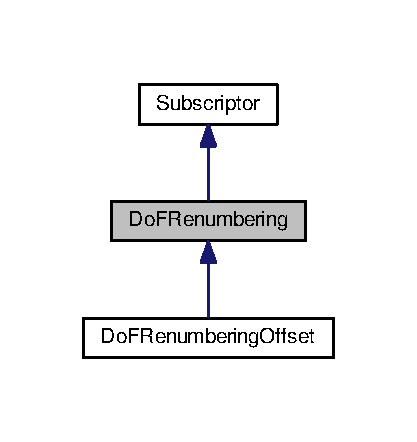
\includegraphics[width=211pt]{class_do_f_renumbering__inherit__graph}
\end{center}
\end{figure}


Collaboration diagram for Do\+F\+Renumbering\+:\nopagebreak
\begin{figure}[H]
\begin{center}
\leavevmode
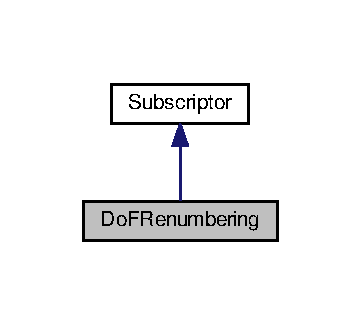
\includegraphics[width=181pt]{class_do_f_renumbering__coll__graph}
\end{center}
\end{figure}
\doxysubsection*{Public Member Functions}
\begin{DoxyCompactItemize}
\item 
virtual void \mbox{\hyperlink{class_do_f_renumbering_a3dd9e72a14b3078a9f823222eacd162c}{convert\+\_\+dof\+\_\+indices}} (std\+::vector$<$ unsigned int $>$ \&dof\+\_\+indices) const
\item 
virtual std\+::vector$<$ std\+::pair$<$ const unsigned int, const unsigned int $>$ $>$ \mbox{\hyperlink{class_do_f_renumbering_a39be83786966bdce332a902104993c74}{convert\+\_\+range}} (const unsigned int range\+\_\+begin, const unsigned int range\+\_\+end) const
\item 
virtual \mbox{\hyperlink{class_do_f_renumbering_a0443d7cb614fa161e4201ff7a6bdf541}{$\sim$\+Do\+F\+Renumbering}} ()
\end{DoxyCompactItemize}
\doxysubsection*{Additional Inherited Members}


\doxysubsection{Detailed Description}
This class is intended to describe a renumbering of dof indices

The class inherits from \textbf{ Subscriptor} in order to be able to check that \mbox{\hyperlink{class_do_f_renumbering}{Do\+F\+Renumbering}} objects are only destroyed when they are not needed anymore by other objects.

The default implementation does no renumbering. 

\doxysubsection{Constructor \& Destructor Documentation}
\mbox{\Hypertarget{class_do_f_renumbering_a0443d7cb614fa161e4201ff7a6bdf541}\label{class_do_f_renumbering_a0443d7cb614fa161e4201ff7a6bdf541}} 
\index{DoFRenumbering@{DoFRenumbering}!````~DoFRenumbering@{$\sim$DoFRenumbering}}
\index{````~DoFRenumbering@{$\sim$DoFRenumbering}!DoFRenumbering@{DoFRenumbering}}
\doxysubsubsection{\texorpdfstring{$\sim$DoFRenumbering()}{~DoFRenumbering()}}
{\footnotesize\ttfamily virtual Do\+F\+Renumbering\+::$\sim$\+Do\+F\+Renumbering (\begin{DoxyParamCaption}{ }\end{DoxyParamCaption})\hspace{0.3cm}{\ttfamily [virtual]}}

The destructor of \mbox{\hyperlink{class_do_f_renumbering}{Do\+F\+Renumbering}} essentially checks before destruction that the \mbox{\hyperlink{class_do_f_renumbering}{Do\+F\+Renumbering}} object is not used by other objects. If this is the case, the program will be aborted. 

\doxysubsection{Member Function Documentation}
\mbox{\Hypertarget{class_do_f_renumbering_a3dd9e72a14b3078a9f823222eacd162c}\label{class_do_f_renumbering_a3dd9e72a14b3078a9f823222eacd162c}} 
\index{DoFRenumbering@{DoFRenumbering}!convert\_dof\_indices@{convert\_dof\_indices}}
\index{convert\_dof\_indices@{convert\_dof\_indices}!DoFRenumbering@{DoFRenumbering}}
\doxysubsubsection{\texorpdfstring{convert\_dof\_indices()}{convert\_dof\_indices()}}
{\footnotesize\ttfamily virtual void Do\+F\+Renumbering\+::convert\+\_\+dof\+\_\+indices (\begin{DoxyParamCaption}\item[{std\+::vector$<$ unsigned int $>$ \&}]{dof\+\_\+indices }\end{DoxyParamCaption}) const\hspace{0.3cm}{\ttfamily [virtual]}}

This function renumbers the incoming dof indices


\begin{DoxyParams}[1]{Parameters}
\mbox{\texttt{ in,out}}  & {\em dof\+\_\+indices} & The vector with the dof indices to be renumbered \\
\hline
\end{DoxyParams}


Reimplemented in \mbox{\hyperlink{class_do_f_renumbering_offset_a11744a010a6502ae0aa9bac11c7ff3f0}{Do\+F\+Renumbering\+Offset}}.

\mbox{\Hypertarget{class_do_f_renumbering_a39be83786966bdce332a902104993c74}\label{class_do_f_renumbering_a39be83786966bdce332a902104993c74}} 
\index{DoFRenumbering@{DoFRenumbering}!convert\_range@{convert\_range}}
\index{convert\_range@{convert\_range}!DoFRenumbering@{DoFRenumbering}}
\doxysubsubsection{\texorpdfstring{convert\_range()}{convert\_range()}}
{\footnotesize\ttfamily virtual std\+::vector$<$std\+::pair$<$const unsigned int, const unsigned int$>$ $>$ Do\+F\+Renumbering\+::convert\+\_\+range (\begin{DoxyParamCaption}\item[{const unsigned int}]{range\+\_\+begin,  }\item[{const unsigned int}]{range\+\_\+end }\end{DoxyParamCaption}) const\hspace{0.3cm}{\ttfamily [virtual]}}

Converts a contiguous range \mbox{[}{\ttfamily range\+\_\+begin}, {\ttfamily range\+\_\+end}\mbox{]} of indices into one or several contiguous ranges in the new numbering


\begin{DoxyParams}[1]{Parameters}
\mbox{\texttt{ in}}  & {\em range\+\_\+begin} & First index\\
\hline
\mbox{\texttt{ in}}  & {\em range\+\_\+end} & Past the last index\\
\hline
\end{DoxyParams}
\begin{DoxyReturn}{Returns}
A vector with one or several ranges. 
\end{DoxyReturn}


Reimplemented in \mbox{\hyperlink{class_do_f_renumbering_offset_adef238432ea7b8100c3d4d0e008a9f72}{Do\+F\+Renumbering\+Offset}}.



The documentation for this class was generated from the following file\+:\begin{DoxyCompactItemize}
\item 
/home/sst/code/\+Galerkin\+Tools/\+Galerkin\+Tools/include/galerkin\+\_\+tools/\mbox{\hyperlink{dof__renumbering_8h}{dof\+\_\+renumbering.\+h}}\end{DoxyCompactItemize}

\hypertarget{class_do_f_renumbering_offset}{}\section{Do\+F\+Renumbering\+Offset Class Reference}
\label{class_do_f_renumbering_offset}\index{Do\+F\+Renumbering\+Offset@{Do\+F\+Renumbering\+Offset}}


{\ttfamily \#include $<$dof\+\_\+renumbering.\+h$>$}



Inheritance diagram for Do\+F\+Renumbering\+Offset\+:\nopagebreak
\begin{figure}[H]
\begin{center}
\leavevmode
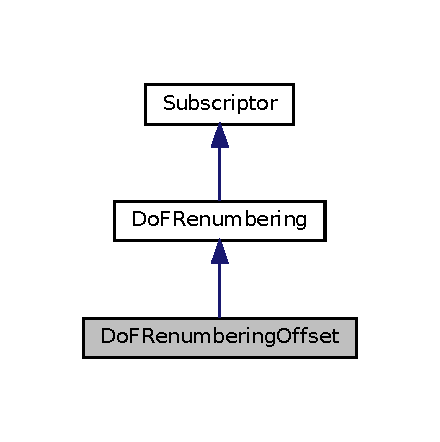
\includegraphics[width=200pt]{class_do_f_renumbering_offset__inherit__graph}
\end{center}
\end{figure}


Collaboration diagram for Do\+F\+Renumbering\+Offset\+:\nopagebreak
\begin{figure}[H]
\begin{center}
\leavevmode
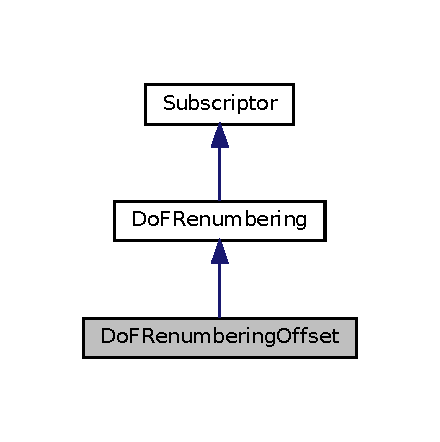
\includegraphics[width=200pt]{class_do_f_renumbering_offset__coll__graph}
\end{center}
\end{figure}
\subsection*{Public Member Functions}
\begin{DoxyCompactItemize}
\item 
void \hyperlink{class_do_f_renumbering_offset_a39333b4c3597c2b4a967f7af3cec0054}{add\+\_\+range} (const unsigned int dof\+\_\+start, const unsigned int dof\+\_\+end, const int offset)
\item 
virtual void \hyperlink{class_do_f_renumbering_offset_a7b48f6f59b90c015b7e176148edbb797}{convert\+\_\+dof\+\_\+indices} (std\+::vector$<$ unsigned int $>$ \&dof\+\_\+indices) const 
\item 
virtual std\+::vector$<$ std\+::pair$<$ const unsigned int, const unsigned int $>$ $>$ \hyperlink{class_do_f_renumbering_offset_ac066233b202f7982d29206c1221c1f6a}{convert\+\_\+range} (const unsigned int range\+\_\+begin, const unsigned int range\+\_\+end) const 
\item 
const std\+::vector$<$ std\+::tuple$<$ const unsigned int, const unsigned int, const int $>$ $>$ \& \hyperlink{class_do_f_renumbering_offset_af92a21719157c5fd5e8ae42cf8af87f6}{get\+\_\+dof\+\_\+offsets} () const 
\item 
void \hyperlink{class_do_f_renumbering_offset_ac7156c58d0aa5dcb57fa0fe3ac437453}{clear} ()
\item 
void \hyperlink{class_do_f_renumbering_offset_a51ae1b70be0b0a2444c4bba71a272f71}{print} (std\+::ostream \&out) const 
\end{DoxyCompactItemize}
\subsection*{Private Attributes}
\begin{DoxyCompactItemize}
\item 
std\+::vector$<$ std\+::tuple$<$ const unsigned int, const unsigned int, const int $>$ $>$ \hyperlink{class_do_f_renumbering_offset_a5df6c4b70b1394c3670ced634146c9a9}{dof\+\_\+offsets}
\end{DoxyCompactItemize}
\subsection*{Additional Inherited Members}


\subsection{Detailed Description}
This renumbering scheme is based on applying offsets to index ranges. Presently no measures are taken to ensure that the overall index set is consistent! 

\subsection{Member Function Documentation}
\index{Do\+F\+Renumbering\+Offset@{Do\+F\+Renumbering\+Offset}!add\+\_\+range@{add\+\_\+range}}
\index{add\+\_\+range@{add\+\_\+range}!Do\+F\+Renumbering\+Offset@{Do\+F\+Renumbering\+Offset}}
\subsubsection[{\texorpdfstring{add\+\_\+range(const unsigned int dof\+\_\+start, const unsigned int dof\+\_\+end, const int offset)}{add_range(const unsigned int dof_start, const unsigned int dof_end, const int offset)}}]{\setlength{\rightskip}{0pt plus 5cm}void Do\+F\+Renumbering\+Offset\+::add\+\_\+range (
\begin{DoxyParamCaption}
\item[{const unsigned int}]{dof\+\_\+start, }
\item[{const unsigned int}]{dof\+\_\+end, }
\item[{const int}]{offset}
\end{DoxyParamCaption}
)}\hypertarget{class_do_f_renumbering_offset_a39333b4c3597c2b4a967f7af3cec0054}{}\label{class_do_f_renumbering_offset_a39333b4c3597c2b4a967f7af3cec0054}
Add an element to \hyperlink{class_do_f_renumbering_offset_a5df6c4b70b1394c3670ced634146c9a9}{Do\+F\+Renumbering\+Offset\+::dof\+\_\+offsets}


\begin{DoxyParams}[1]{Parameters}
\mbox{\tt in}  & {\em dof\+\_\+start} & The first index of the original interval\\
\hline
\mbox{\tt in}  & {\em dof\+\_\+end} & The last index of the original interval (or, rather, the index past the last index)\\
\hline
\mbox{\tt in}  & {\em offset} & The offset to be applied \\
\hline
\end{DoxyParams}
\index{Do\+F\+Renumbering\+Offset@{Do\+F\+Renumbering\+Offset}!clear@{clear}}
\index{clear@{clear}!Do\+F\+Renumbering\+Offset@{Do\+F\+Renumbering\+Offset}}
\subsubsection[{\texorpdfstring{clear()}{clear()}}]{\setlength{\rightskip}{0pt plus 5cm}void Do\+F\+Renumbering\+Offset\+::clear (
\begin{DoxyParamCaption}
{}
\end{DoxyParamCaption}
)}\hypertarget{class_do_f_renumbering_offset_ac7156c58d0aa5dcb57fa0fe3ac437453}{}\label{class_do_f_renumbering_offset_ac7156c58d0aa5dcb57fa0fe3ac437453}
Function resetting the object \index{Do\+F\+Renumbering\+Offset@{Do\+F\+Renumbering\+Offset}!convert\+\_\+dof\+\_\+indices@{convert\+\_\+dof\+\_\+indices}}
\index{convert\+\_\+dof\+\_\+indices@{convert\+\_\+dof\+\_\+indices}!Do\+F\+Renumbering\+Offset@{Do\+F\+Renumbering\+Offset}}
\subsubsection[{\texorpdfstring{convert\+\_\+dof\+\_\+indices(std\+::vector$<$ unsigned int $>$ \&dof\+\_\+indices) const }{convert_dof_indices(std::vector< unsigned int > &dof_indices) const }}]{\setlength{\rightskip}{0pt plus 5cm}virtual void Do\+F\+Renumbering\+Offset\+::convert\+\_\+dof\+\_\+indices (
\begin{DoxyParamCaption}
\item[{std\+::vector$<$ unsigned int $>$ \&}]{dof\+\_\+indices}
\end{DoxyParamCaption}
) const\hspace{0.3cm}{\ttfamily [virtual]}}\hypertarget{class_do_f_renumbering_offset_a7b48f6f59b90c015b7e176148edbb797}{}\label{class_do_f_renumbering_offset_a7b48f6f59b90c015b7e176148edbb797}
This function renumbers the incoming dof indices


\begin{DoxyParams}[1]{Parameters}
\mbox{\tt in,out}  & {\em dof\+\_\+indices} & The vector with the dof indices to be renumbered \\
\hline
\end{DoxyParams}


Reimplemented from \hyperlink{class_do_f_renumbering_ad37a052986c62df79a1ebc8abea13e89}{Do\+F\+Renumbering}.

\index{Do\+F\+Renumbering\+Offset@{Do\+F\+Renumbering\+Offset}!convert\+\_\+range@{convert\+\_\+range}}
\index{convert\+\_\+range@{convert\+\_\+range}!Do\+F\+Renumbering\+Offset@{Do\+F\+Renumbering\+Offset}}
\subsubsection[{\texorpdfstring{convert\+\_\+range(const unsigned int range\+\_\+begin, const unsigned int range\+\_\+end) const }{convert_range(const unsigned int range_begin, const unsigned int range_end) const }}]{\setlength{\rightskip}{0pt plus 5cm}virtual std\+::vector$<$std\+::pair$<$const unsigned int, const unsigned int$>$ $>$ Do\+F\+Renumbering\+Offset\+::convert\+\_\+range (
\begin{DoxyParamCaption}
\item[{const unsigned int}]{range\+\_\+begin, }
\item[{const unsigned int}]{range\+\_\+end}
\end{DoxyParamCaption}
) const\hspace{0.3cm}{\ttfamily [virtual]}}\hypertarget{class_do_f_renumbering_offset_ac066233b202f7982d29206c1221c1f6a}{}\label{class_do_f_renumbering_offset_ac066233b202f7982d29206c1221c1f6a}
Converts a contiguous range \mbox{[}{\ttfamily range\+\_\+begin}, {\ttfamily range\+\_\+end}\mbox{]} of indices into one or several contiguous ranges in the new numbering


\begin{DoxyParams}[1]{Parameters}
\mbox{\tt in}  & {\em range\+\_\+begin} & First index\\
\hline
\mbox{\tt in}  & {\em range\+\_\+end} & Past the last index\\
\hline
\end{DoxyParams}
\begin{DoxyReturn}{Returns}
A vector with one or several ranges. 
\end{DoxyReturn}


Reimplemented from \hyperlink{class_do_f_renumbering_ae95ba2f7f04a172812f086fc75b61c15}{Do\+F\+Renumbering}.

\index{Do\+F\+Renumbering\+Offset@{Do\+F\+Renumbering\+Offset}!get\+\_\+dof\+\_\+offsets@{get\+\_\+dof\+\_\+offsets}}
\index{get\+\_\+dof\+\_\+offsets@{get\+\_\+dof\+\_\+offsets}!Do\+F\+Renumbering\+Offset@{Do\+F\+Renumbering\+Offset}}
\subsubsection[{\texorpdfstring{get\+\_\+dof\+\_\+offsets() const }{get_dof_offsets() const }}]{\setlength{\rightskip}{0pt plus 5cm}const std\+::vector$<$std\+::tuple$<$const unsigned int, const unsigned int, const int$>$ $>$\& Do\+F\+Renumbering\+Offset\+::get\+\_\+dof\+\_\+offsets (
\begin{DoxyParamCaption}
{}
\end{DoxyParamCaption}
) const}\hypertarget{class_do_f_renumbering_offset_af92a21719157c5fd5e8ae42cf8af87f6}{}\label{class_do_f_renumbering_offset_af92a21719157c5fd5e8ae42cf8af87f6}
\begin{DoxyReturn}{Returns}
\hyperlink{class_do_f_renumbering_offset_a5df6c4b70b1394c3670ced634146c9a9}{Do\+F\+Renumbering\+Offset\+::dof\+\_\+offsets} 
\end{DoxyReturn}
\index{Do\+F\+Renumbering\+Offset@{Do\+F\+Renumbering\+Offset}!print@{print}}
\index{print@{print}!Do\+F\+Renumbering\+Offset@{Do\+F\+Renumbering\+Offset}}
\subsubsection[{\texorpdfstring{print(std\+::ostream \&out) const }{print(std::ostream &out) const }}]{\setlength{\rightskip}{0pt plus 5cm}void Do\+F\+Renumbering\+Offset\+::print (
\begin{DoxyParamCaption}
\item[{std\+::ostream \&}]{out}
\end{DoxyParamCaption}
) const}\hypertarget{class_do_f_renumbering_offset_a51ae1b70be0b0a2444c4bba71a272f71}{}\label{class_do_f_renumbering_offset_a51ae1b70be0b0a2444c4bba71a272f71}
print the renumbering scheme to screen


\begin{DoxyParams}[1]{Parameters}
\mbox{\tt in}  & {\em out} & The output stream \\
\hline
\end{DoxyParams}


\subsection{Member Data Documentation}
\index{Do\+F\+Renumbering\+Offset@{Do\+F\+Renumbering\+Offset}!dof\+\_\+offsets@{dof\+\_\+offsets}}
\index{dof\+\_\+offsets@{dof\+\_\+offsets}!Do\+F\+Renumbering\+Offset@{Do\+F\+Renumbering\+Offset}}
\subsubsection[{\texorpdfstring{dof\+\_\+offsets}{dof_offsets}}]{\setlength{\rightskip}{0pt plus 5cm}std\+::vector$<$std\+::tuple$<$const unsigned int, const unsigned int, const int$>$ $>$ Do\+F\+Renumbering\+Offset\+::dof\+\_\+offsets\hspace{0.3cm}{\ttfamily [private]}}\hypertarget{class_do_f_renumbering_offset_a5df6c4b70b1394c3670ced634146c9a9}{}\label{class_do_f_renumbering_offset_a5df6c4b70b1394c3670ced634146c9a9}
This data structure defines a fixed shift of dof numbers from a certain interval \mbox{[}dof\+\_\+start\+\_\+i, dof\+\_\+end\+\_\+i\mbox{]} to the interval \mbox{[}dof\+\_\+start\+\_\+i + offset\+\_\+i, dof\+\_\+end\+\_\+i + offset\+\_\+i\mbox{]}. The tuples (dof\+\_\+start\+\_\+i, dof\+\_\+end\+\_\+i, offset\+\_\+i) define this shift. Multiple intervals can be added and the order of adding the intervals influences how the intervals are searched during conversion of dof indices. In particular, if a certain dof index is to be converted, it is initially tried to find it in the interval added first, if it is not found there, the second interval is tried, and so forth.\begin{DoxyRefDesc}{Todo}
\item[\hyperlink{todo__todo000009}{Todo}]It would be worthwhile to implement a more effective conversion scheme. \end{DoxyRefDesc}


The documentation for this class was generated from the following file\+:\begin{DoxyCompactItemize}
\item 
/home/sst/\+F\+E/code/incremental\+F\+E/galerkin\+\_\+tools/include/galerkin\+\_\+tools/\hyperlink{dof__renumbering_8h}{dof\+\_\+renumbering.\+h}\end{DoxyCompactItemize}

\hypertarget{class_domain_cell_do_f_iterator}{}\section{Domain\+Cell\+Do\+F\+Iterator$<$ spacedim $>$ Class Template Reference}
\label{class_domain_cell_do_f_iterator}\index{Domain\+Cell\+Do\+F\+Iterator$<$ spacedim $>$@{Domain\+Cell\+Do\+F\+Iterator$<$ spacedim $>$}}


{\ttfamily \#include $<$dof\+\_\+handler\+\_\+system.\+h$>$}



Inheritance diagram for Domain\+Cell\+Do\+F\+Iterator$<$ spacedim $>$\+:\nopagebreak
\begin{figure}[H]
\begin{center}
\leavevmode
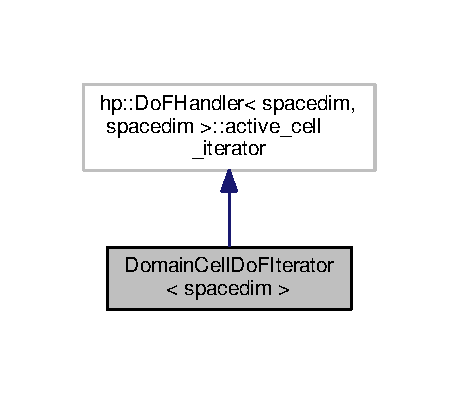
\includegraphics[width=220pt]{class_domain_cell_do_f_iterator__inherit__graph}
\end{center}
\end{figure}


Collaboration diagram for Domain\+Cell\+Do\+F\+Iterator$<$ spacedim $>$\+:\nopagebreak
\begin{figure}[H]
\begin{center}
\leavevmode
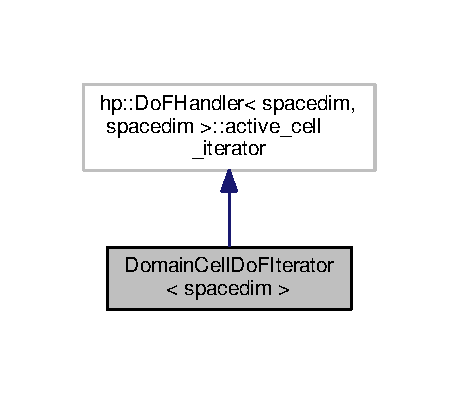
\includegraphics[width=220pt]{class_domain_cell_do_f_iterator__coll__graph}
\end{center}
\end{figure}
\subsection*{Public Member Functions}
\begin{DoxyCompactItemize}
\item 
\hyperlink{class_domain_cell_do_f_iterator_a36416883d4c91dd0849520d3e205dba1}{Domain\+Cell\+Do\+F\+Iterator} (const {\bf Tria\+Iterator}$<$ {\bf Cell\+Accessor}$<$ spacedim, spacedim $>$$>$ \&domain\+\_\+cell, const \hyperlink{class_do_f_handler_system}{Do\+F\+Handler\+System}$<$ spacedim $>$ \&\hyperlink{class_domain_cell_do_f_iterator_a7431a0505f1e5b0b796c7f58cf9a060c}{dof\+\_\+handler\+\_\+system})
\item 
\hyperlink{class_domain_cell_do_f_iterator_a4e987bc73bb2c8ec6974cc6427505091}{Domain\+Cell\+Do\+F\+Iterator} (const \hyperlink{class_do_f_handler_system}{Do\+F\+Handler\+System}$<$ spacedim $>$ \&\hyperlink{class_domain_cell_do_f_iterator_a7431a0505f1e5b0b796c7f58cf9a060c}{dof\+\_\+handler\+\_\+system})
\item 
void \hyperlink{class_domain_cell_do_f_iterator_ad93f1a26a4efd4ca94af45d13e250aba}{get\+\_\+dof\+\_\+indices} (std\+::vector$<$ {\bf types\+::global\+\_\+dof\+\_\+index} $>$ \&dof\+\_\+indices) const 
\end{DoxyCompactItemize}
\subsection*{Private Attributes}
\begin{DoxyCompactItemize}
\item 
const \hyperlink{class_do_f_handler_system}{Do\+F\+Handler\+System}$<$ spacedim $>$ \& \hyperlink{class_domain_cell_do_f_iterator_a7431a0505f1e5b0b796c7f58cf9a060c}{dof\+\_\+handler\+\_\+system}
\end{DoxyCompactItemize}


\subsection{Detailed Description}
\subsubsection*{template$<$unsigned int spacedim$>$\\*
class Domain\+Cell\+Do\+F\+Iterator$<$ spacedim $>$}

This is an active cell iterator (for domain cells) pretty much like the active\+\_\+cell\+\_\+iterator of deal.\+II. However, the difference is that it provides the function \hyperlink{class_domain_cell_do_f_iterator_ad93f1a26a4efd4ca94af45d13e250aba}{Domain\+Cell\+Do\+F\+Iterator\+::get\+\_\+dof\+\_\+indices()}, which returns the dof indices of the cells in the global ordering of the \hyperlink{class_do_f_handler_system}{Do\+F\+Handler\+System} instead of the dof ordering of the deal.\+II dof handler. By using the function domain\+\_\+cell\+\_\+dof\+\_\+iterator.\+get\+\_\+dof\+\_\+indices() you will get the indices in the global ordering of the \hyperlink{class_do_f_handler_system}{Do\+F\+Handler\+System}. In contrast, if you use domain\+\_\+cell\+\_\+dof\+\_\+iterator-\/$>$\hyperlink{class_domain_cell_do_f_iterator_ad93f1a26a4efd4ca94af45d13e250aba}{get\+\_\+dof\+\_\+indices()}, you get the indices in the ordering of the deal.\+II dof handler. 

\subsection{Constructor \& Destructor Documentation}
\index{Domain\+Cell\+Do\+F\+Iterator@{Domain\+Cell\+Do\+F\+Iterator}!Domain\+Cell\+Do\+F\+Iterator@{Domain\+Cell\+Do\+F\+Iterator}}
\index{Domain\+Cell\+Do\+F\+Iterator@{Domain\+Cell\+Do\+F\+Iterator}!Domain\+Cell\+Do\+F\+Iterator@{Domain\+Cell\+Do\+F\+Iterator}}
\subsubsection[{\texorpdfstring{Domain\+Cell\+Do\+F\+Iterator(const Tria\+Iterator$<$ Cell\+Accessor$<$ spacedim, spacedim $>$$>$ \&domain\+\_\+cell, const Do\+F\+Handler\+System$<$ spacedim $>$ \&dof\+\_\+handler\+\_\+system)}{DomainCellDoFIterator(const TriaIterator< CellAccessor< spacedim, spacedim >> &domain_cell, const DoFHandlerSystem< spacedim > &dof_handler_system)}}]{\setlength{\rightskip}{0pt plus 5cm}template$<$unsigned int spacedim$>$ {\bf Domain\+Cell\+Do\+F\+Iterator}$<$ spacedim $>$\+::{\bf Domain\+Cell\+Do\+F\+Iterator} (
\begin{DoxyParamCaption}
\item[{const {\bf Tria\+Iterator}$<$ {\bf Cell\+Accessor}$<$ spacedim, spacedim $>$$>$ \&}]{domain\+\_\+cell, }
\item[{const {\bf Do\+F\+Handler\+System}$<$ spacedim $>$ \&}]{dof\+\_\+handler\+\_\+system}
\end{DoxyParamCaption}
)}\hypertarget{class_domain_cell_do_f_iterator_a36416883d4c91dd0849520d3e205dba1}{}\label{class_domain_cell_do_f_iterator_a36416883d4c91dd0849520d3e205dba1}
Constructor


\begin{DoxyParams}[1]{Parameters}
\mbox{\tt in}  & {\em domain\+\_\+cell} & The domain cell of the triangulation\\
\hline
\mbox{\tt in}  & {\em dof\+\_\+handler\+\_\+system} & The underlying \hyperlink{class_do_f_handler_system}{Do\+F\+Handler\+System} \\
\hline
\end{DoxyParams}
\index{Domain\+Cell\+Do\+F\+Iterator@{Domain\+Cell\+Do\+F\+Iterator}!Domain\+Cell\+Do\+F\+Iterator@{Domain\+Cell\+Do\+F\+Iterator}}
\index{Domain\+Cell\+Do\+F\+Iterator@{Domain\+Cell\+Do\+F\+Iterator}!Domain\+Cell\+Do\+F\+Iterator@{Domain\+Cell\+Do\+F\+Iterator}}
\subsubsection[{\texorpdfstring{Domain\+Cell\+Do\+F\+Iterator(const Do\+F\+Handler\+System$<$ spacedim $>$ \&dof\+\_\+handler\+\_\+system)}{DomainCellDoFIterator(const DoFHandlerSystem< spacedim > &dof_handler_system)}}]{\setlength{\rightskip}{0pt plus 5cm}template$<$unsigned int spacedim$>$ {\bf Domain\+Cell\+Do\+F\+Iterator}$<$ spacedim $>$\+::{\bf Domain\+Cell\+Do\+F\+Iterator} (
\begin{DoxyParamCaption}
\item[{const {\bf Do\+F\+Handler\+System}$<$ spacedim $>$ \&}]{dof\+\_\+handler\+\_\+system}
\end{DoxyParamCaption}
)}\hypertarget{class_domain_cell_do_f_iterator_a4e987bc73bb2c8ec6974cc6427505091}{}\label{class_domain_cell_do_f_iterator_a4e987bc73bb2c8ec6974cc6427505091}
Constructor for the end() element


\begin{DoxyParams}[1]{Parameters}
\mbox{\tt in}  & {\em dof\+\_\+handler\+\_\+system} & The underlying \hyperlink{class_do_f_handler_system}{Do\+F\+Handler\+System} \\
\hline
\end{DoxyParams}


\subsection{Member Function Documentation}
\index{Domain\+Cell\+Do\+F\+Iterator@{Domain\+Cell\+Do\+F\+Iterator}!get\+\_\+dof\+\_\+indices@{get\+\_\+dof\+\_\+indices}}
\index{get\+\_\+dof\+\_\+indices@{get\+\_\+dof\+\_\+indices}!Domain\+Cell\+Do\+F\+Iterator@{Domain\+Cell\+Do\+F\+Iterator}}
\subsubsection[{\texorpdfstring{get\+\_\+dof\+\_\+indices(std\+::vector$<$ types\+::global\+\_\+dof\+\_\+index $>$ \&dof\+\_\+indices) const }{get_dof_indices(std::vector< types::global_dof_index > &dof_indices) const }}]{\setlength{\rightskip}{0pt plus 5cm}template$<$unsigned int spacedim$>$ void {\bf Domain\+Cell\+Do\+F\+Iterator}$<$ spacedim $>$\+::get\+\_\+dof\+\_\+indices (
\begin{DoxyParamCaption}
\item[{std\+::vector$<$ {\bf types\+::global\+\_\+dof\+\_\+index} $>$ \&}]{dof\+\_\+indices}
\end{DoxyParamCaption}
) const}\hypertarget{class_domain_cell_do_f_iterator_ad93f1a26a4efd4ca94af45d13e250aba}{}\label{class_domain_cell_do_f_iterator_ad93f1a26a4efd4ca94af45d13e250aba}
Function returning the dof indices in the global ordering of the dof handler system \hyperlink{class_domain_cell_do_f_iterator_a7431a0505f1e5b0b796c7f58cf9a060c}{Domain\+Cell\+Do\+F\+Iterator\+::dof\+\_\+handler\+\_\+system}


\begin{DoxyParams}[1]{Parameters}
\mbox{\tt out}  & {\em dof\+\_\+indices} & The returned dof indices \\
\hline
\end{DoxyParams}


\subsection{Member Data Documentation}
\index{Domain\+Cell\+Do\+F\+Iterator@{Domain\+Cell\+Do\+F\+Iterator}!dof\+\_\+handler\+\_\+system@{dof\+\_\+handler\+\_\+system}}
\index{dof\+\_\+handler\+\_\+system@{dof\+\_\+handler\+\_\+system}!Domain\+Cell\+Do\+F\+Iterator@{Domain\+Cell\+Do\+F\+Iterator}}
\subsubsection[{\texorpdfstring{dof\+\_\+handler\+\_\+system}{dof_handler_system}}]{\setlength{\rightskip}{0pt plus 5cm}template$<$unsigned int spacedim$>$ const {\bf Do\+F\+Handler\+System}$<$spacedim$>$\& {\bf Domain\+Cell\+Do\+F\+Iterator}$<$ spacedim $>$\+::dof\+\_\+handler\+\_\+system\hspace{0.3cm}{\ttfamily [private]}}\hypertarget{class_domain_cell_do_f_iterator_a7431a0505f1e5b0b796c7f58cf9a060c}{}\label{class_domain_cell_do_f_iterator_a7431a0505f1e5b0b796c7f58cf9a060c}
The underlying \hyperlink{class_do_f_handler_system}{Do\+F\+Handler\+System} 

The documentation for this class was generated from the following file\+:\begin{DoxyCompactItemize}
\item 
/home/sst/code/\+Galerkin\+Tools/\+Galerkin\+Tools/include/galerkin\+\_\+tools/\hyperlink{dof__handler__system_8h}{dof\+\_\+handler\+\_\+system.\+h}\end{DoxyCompactItemize}

\hypertarget{class_f_e_values_interface}{}\doxysection{FEValues\+Interface$<$ spacedim $>$ Class Template Reference}
\label{class_f_e_values_interface}\index{FEValuesInterface$<$ spacedim $>$@{FEValuesInterface$<$ spacedim $>$}}


{\ttfamily \#include $<$fe\+\_\+values\+\_\+interface.\+h$>$}



Collaboration diagram for FEValues\+Interface$<$ spacedim $>$\+:\nopagebreak
\begin{figure}[H]
\begin{center}
\leavevmode
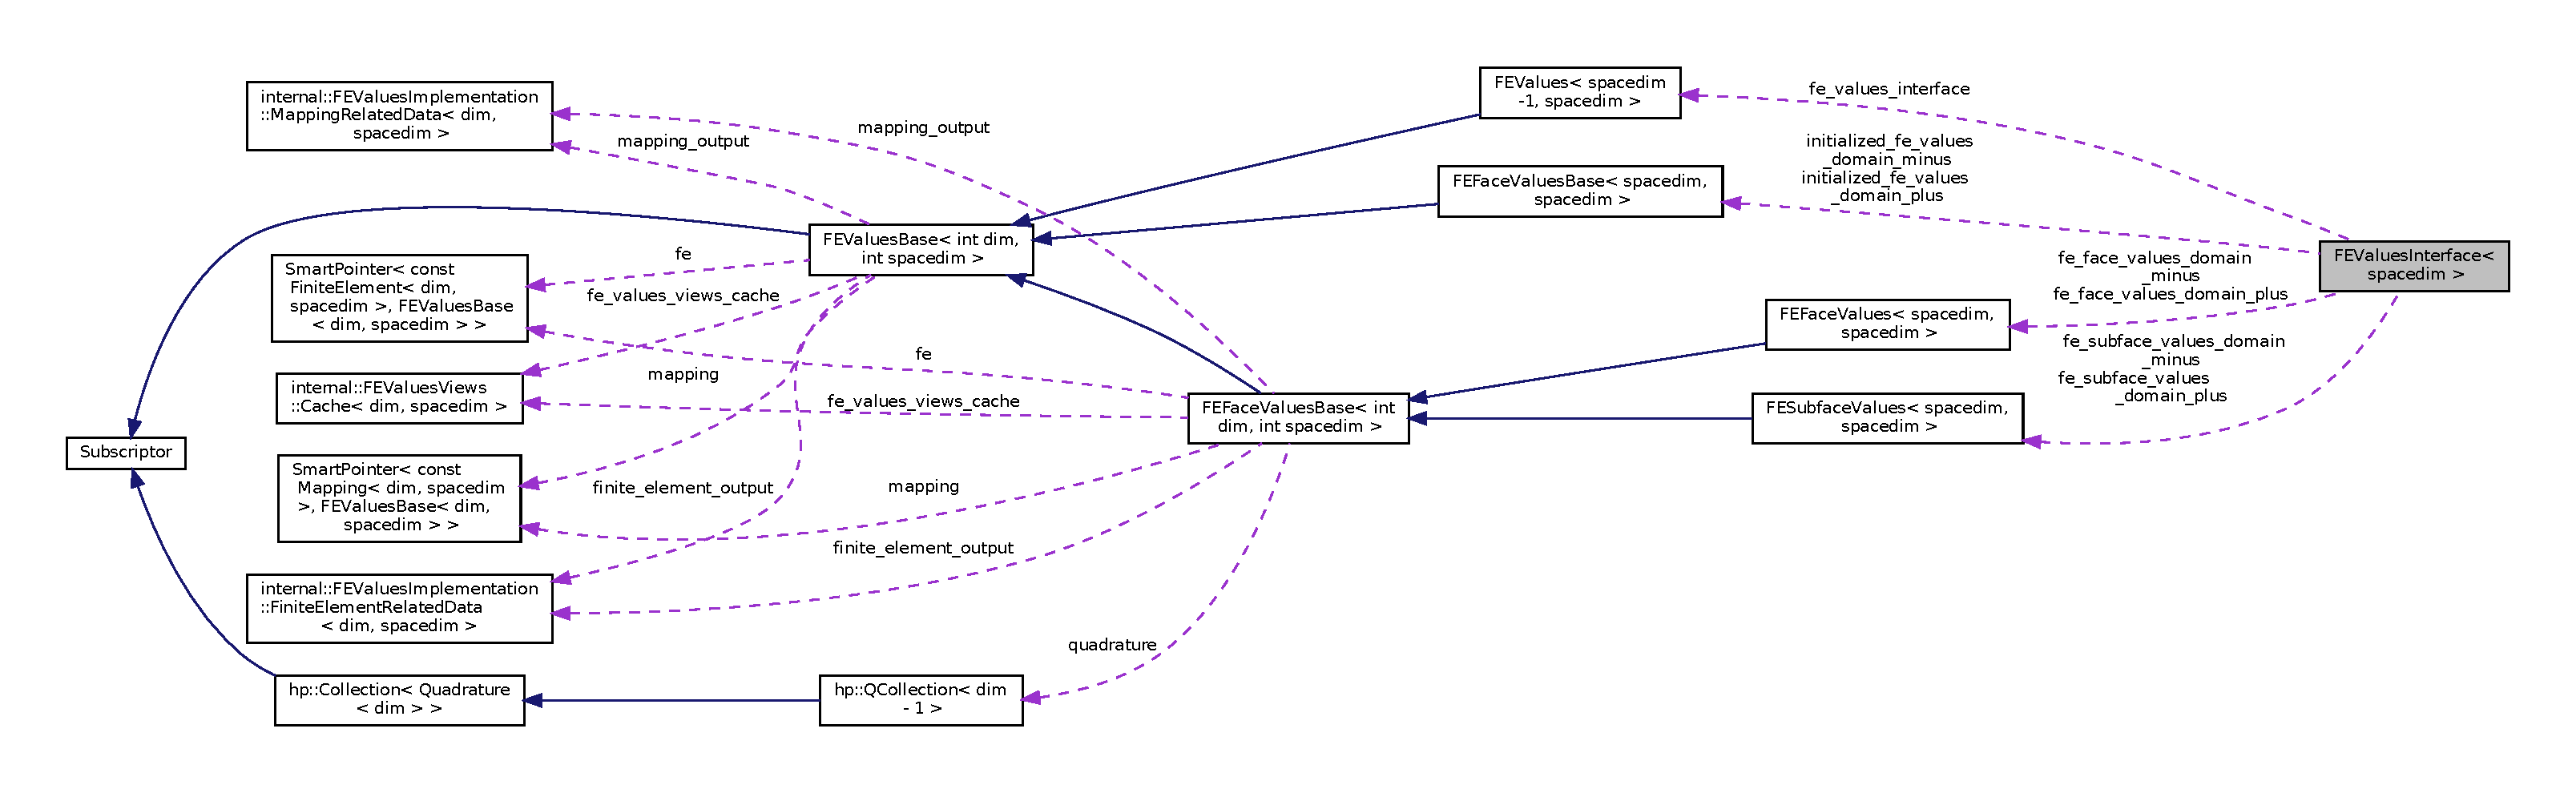
\includegraphics[width=350pt]{class_f_e_values_interface__coll__graph}
\end{center}
\end{figure}
\doxysubsection*{Public Member Functions}
\begin{DoxyCompactItemize}
\item 
\mbox{\hyperlink{class_f_e_values_interface_ae48863eabc0754e1cc033143fcd2d443}{FEValues\+Interface}} (const \textbf{ Mapping}$<$ spacedim-\/1, spacedim $>$ \&mapping\+\_\+interface, const \textbf{ Mapping}$<$ spacedim, spacedim $>$ \&mapping\+\_\+domain, const \textbf{ Finite\+Element}$<$ spacedim-\/1, spacedim $>$ \&fe\+\_\+interface, const \textbf{ Finite\+Element}$<$ spacedim, spacedim $>$ \&fe\+\_\+domain\+\_\+minus, const \textbf{ Finite\+Element}$<$ spacedim, spacedim $>$ \&fe\+\_\+domain\+\_\+plus, const \textbf{ Quadrature}$<$ spacedim-\/1 $>$ \&quadrature, const \textbf{ Update\+Flags} update\+\_\+flags\+\_\+interface, const \textbf{ Update\+Flags} update\+\_\+flags\+\_\+domain\+\_\+minus, const \textbf{ Update\+Flags} update\+\_\+flags\+\_\+domain\+\_\+plus)
\item 
void \mbox{\hyperlink{class_f_e_values_interface_a334ed0ef179516854690e7e3fa273aa0}{reinit}} (const \mbox{\hyperlink{class_interface_cell_domain_cells_do_f}{Interface\+Cell\+Domain\+Cells\+DoF}}$<$ spacedim $>$ \&interface\+\_\+cell\+\_\+domain\+\_\+cells)
\item 
void \mbox{\hyperlink{class_f_e_values_interface_a875a17d471069ddb97cbd8e6f7aba2b8}{reinit}} (const \mbox{\hyperlink{class_interface_cell_domain_cells}{Interface\+Cell\+Domain\+Cells}}$<$ spacedim $>$ \&interface\+\_\+cell\+\_\+domain\+\_\+cells)
\item 
const \textbf{ Quadrature}$<$ spacedim-\/1 $>$ \& \mbox{\hyperlink{class_f_e_values_interface_abbaae0efa290c18b4ecfabc90b151136}{get\+\_\+quadrature}} () const
\item 
const \textbf{ FEValues}$<$ spacedim-\/1, spacedim $>$ \& \mbox{\hyperlink{class_f_e_values_interface_a15a3cc642c056496b79e41732f7012c4}{get\+\_\+fe\+\_\+values\+\_\+interface}} () const
\item 
const \textbf{ FEFace\+Values\+Base}$<$ spacedim, spacedim $>$ \& \mbox{\hyperlink{class_f_e_values_interface_a85aeb4a21ad21576d2d550f2d57f3a00}{get\+\_\+fe\+\_\+values\+\_\+domain}} (const \mbox{\hyperlink{triangulation__system_8h_a44f3c00e36c1d6e3c389ae693c09b435}{Interface\+Side}} \&interface\+\_\+side) const
\end{DoxyCompactItemize}
\doxysubsection*{Public Attributes}
\begin{DoxyCompactItemize}
\item 
const unsigned int \mbox{\hyperlink{class_f_e_values_interface_a100afc348b15432f9e241ff56ebffa8d}{n\+\_\+quadrature\+\_\+points}}
\end{DoxyCompactItemize}
\doxysubsection*{Private Attributes}
\begin{DoxyCompactItemize}
\item 
\mbox{\hyperlink{triangulation__system_8h_a4cfb8c5e21535951e919b6a6b1023af7}{Interface\+Refinement\+Case}} \mbox{\hyperlink{class_f_e_values_interface_a4a14b4fa181df533a6c7e7971fad5c4e}{initialized\+\_\+interface\+\_\+refinement\+\_\+case}}
\item 
const \textbf{ FEFace\+Values\+Base}$<$ spacedim, spacedim $>$ $\ast$ \mbox{\hyperlink{class_f_e_values_interface_a48f1a887c14615d665408f156d879980}{initialized\+\_\+fe\+\_\+values\+\_\+domain\+\_\+minus}} = nullptr
\item 
const \textbf{ FEFace\+Values\+Base}$<$ spacedim, spacedim $>$ $\ast$ \mbox{\hyperlink{class_f_e_values_interface_ab1f7524d517a79cd5e4adbd43017f415}{initialized\+\_\+fe\+\_\+values\+\_\+domain\+\_\+plus}} = nullptr
\item 
\textbf{ FEValues}$<$ spacedim-\/1, spacedim $>$ \mbox{\hyperlink{class_f_e_values_interface_a75f4ee97ebaefa2d1ded52c445953473}{fe\+\_\+values\+\_\+interface}}
\item 
\textbf{ FEFace\+Values}$<$ spacedim, spacedim $>$ \mbox{\hyperlink{class_f_e_values_interface_a1ce4354bfe2e852fdc5b7917614404a7}{fe\+\_\+face\+\_\+values\+\_\+domain\+\_\+minus}}
\item 
\textbf{ FEFace\+Values}$<$ spacedim, spacedim $>$ \mbox{\hyperlink{class_f_e_values_interface_a6d6820b66a2694d327238c6b3c7fb30c}{fe\+\_\+face\+\_\+values\+\_\+domain\+\_\+plus}}
\item 
\textbf{ FESubface\+Values}$<$ spacedim, spacedim $>$ \mbox{\hyperlink{class_f_e_values_interface_abe003c242c807dd162c396d812bbfe77}{fe\+\_\+subface\+\_\+values\+\_\+domain\+\_\+minus}}
\item 
\textbf{ FESubface\+Values}$<$ spacedim, spacedim $>$ \mbox{\hyperlink{class_f_e_values_interface_a184e705efd975db536299ad619585a65}{fe\+\_\+subface\+\_\+values\+\_\+domain\+\_\+plus}}
\end{DoxyCompactItemize}


\doxysubsection{Detailed Description}
\subsubsection*{template$<$unsigned int spacedim$>$\newline
class FEValues\+Interface$<$ spacedim $>$}

This class collects the different \textbf{ FEValues}, \textbf{ FEFace\+Values}, and \textbf{ FESubface\+Values} objects needed for cells at the interface. The situation there is a bit tricky, because, the domain cells adjacent to the interface cell may be refined differently, thus requiring either an \textbf{ FEFace\+Values} or \textbf{ FESubface\+Values} object. This class makes sure that always the correct objects are used. 

\doxysubsection{Constructor \& Destructor Documentation}
\mbox{\Hypertarget{class_f_e_values_interface_ae48863eabc0754e1cc033143fcd2d443}\label{class_f_e_values_interface_ae48863eabc0754e1cc033143fcd2d443}} 
\index{FEValuesInterface$<$ spacedim $>$@{FEValuesInterface$<$ spacedim $>$}!FEValuesInterface@{FEValuesInterface}}
\index{FEValuesInterface@{FEValuesInterface}!FEValuesInterface$<$ spacedim $>$@{FEValuesInterface$<$ spacedim $>$}}
\doxysubsubsection{\texorpdfstring{FEValuesInterface()}{FEValuesInterface()}}
{\footnotesize\ttfamily template$<$unsigned int spacedim$>$ \\
\mbox{\hyperlink{class_f_e_values_interface}{FEValues\+Interface}}$<$ spacedim $>$\+::\mbox{\hyperlink{class_f_e_values_interface}{FEValues\+Interface}} (\begin{DoxyParamCaption}\item[{const \textbf{ Mapping}$<$ spacedim-\/1, spacedim $>$ \&}]{mapping\+\_\+interface,  }\item[{const \textbf{ Mapping}$<$ spacedim, spacedim $>$ \&}]{mapping\+\_\+domain,  }\item[{const \textbf{ Finite\+Element}$<$ spacedim-\/1, spacedim $>$ \&}]{fe\+\_\+interface,  }\item[{const \textbf{ Finite\+Element}$<$ spacedim, spacedim $>$ \&}]{fe\+\_\+domain\+\_\+minus,  }\item[{const \textbf{ Finite\+Element}$<$ spacedim, spacedim $>$ \&}]{fe\+\_\+domain\+\_\+plus,  }\item[{const \textbf{ Quadrature}$<$ spacedim-\/1 $>$ \&}]{quadrature,  }\item[{const \textbf{ Update\+Flags}}]{update\+\_\+flags\+\_\+interface,  }\item[{const \textbf{ Update\+Flags}}]{update\+\_\+flags\+\_\+domain\+\_\+minus,  }\item[{const \textbf{ Update\+Flags}}]{update\+\_\+flags\+\_\+domain\+\_\+plus }\end{DoxyParamCaption})}

The constructor of the class


\begin{DoxyParams}[1]{Parameters}
\mbox{\texttt{ in}}  & {\em mapping\+\_\+interface} & The mapping to be used for the interface cells\\
\hline
\mbox{\texttt{ in}}  & {\em mapping\+\_\+domain} & The mapping to be used for the domain cells\\
\hline
\mbox{\texttt{ in}}  & {\em fe\+\_\+interface} & The finite element for the interface cells\\
\hline
\mbox{\texttt{ in}}  & {\em fe\+\_\+domain\+\_\+minus} & The finite element for the domain cells on the minus side of the interface\\
\hline
\mbox{\texttt{ in}}  & {\em fe\+\_\+domain\+\_\+plus} & The finite element for the domain cells on the plus side of the interface\\
\hline
\mbox{\texttt{ in}}  & {\em quadrature} & The \textbf{ Quadrature} rule to be used\\
\hline
\mbox{\texttt{ in}}  & {\em update\+\_\+flags\+\_\+interface} & \textbf{ Update\+Flags} for the interface cells\\
\hline
\mbox{\texttt{ in}}  & {\em update\+\_\+flags\+\_\+domain\+\_\+minus} & \textbf{ Update\+Flags} for the domain cells on the minus side of interface\\
\hline
\mbox{\texttt{ in}}  & {\em update\+\_\+flags\+\_\+domain\+\_\+plus} & \textbf{ Update\+Flags} for the domain cells on the plus side of interface \\
\hline
\end{DoxyParams}


\doxysubsection{Member Function Documentation}
\mbox{\Hypertarget{class_f_e_values_interface_a85aeb4a21ad21576d2d550f2d57f3a00}\label{class_f_e_values_interface_a85aeb4a21ad21576d2d550f2d57f3a00}} 
\index{FEValuesInterface$<$ spacedim $>$@{FEValuesInterface$<$ spacedim $>$}!get\_fe\_values\_domain@{get\_fe\_values\_domain}}
\index{get\_fe\_values\_domain@{get\_fe\_values\_domain}!FEValuesInterface$<$ spacedim $>$@{FEValuesInterface$<$ spacedim $>$}}
\doxysubsubsection{\texorpdfstring{get\_fe\_values\_domain()}{get\_fe\_values\_domain()}}
{\footnotesize\ttfamily template$<$unsigned int spacedim$>$ \\
const \textbf{ FEFace\+Values\+Base}$<$spacedim,spacedim$>$\& \mbox{\hyperlink{class_f_e_values_interface}{FEValues\+Interface}}$<$ spacedim $>$\+::get\+\_\+fe\+\_\+values\+\_\+domain (\begin{DoxyParamCaption}\item[{const \mbox{\hyperlink{triangulation__system_8h_a44f3c00e36c1d6e3c389ae693c09b435}{Interface\+Side}} \&}]{interface\+\_\+side }\end{DoxyParamCaption}) const}


\begin{DoxyParams}[1]{Parameters}
\mbox{\texttt{ in}}  & {\em interface\+\_\+side} & Either \mbox{\hyperlink{triangulation__system_8h_a44f3c00e36c1d6e3c389ae693c09b435}{Interface\+Side}}\+:\+:{\ttfamily minus} or \mbox{\hyperlink{triangulation__system_8h_a44f3c00e36c1d6e3c389ae693c09b435}{Interface\+Side}}\+:\+:{\ttfamily plus} depending on the side of the interface for which the \textbf{ FEFace\+Values} or \textbf{ FESubface\+Values} is required\\
\hline
\end{DoxyParams}
\begin{DoxyReturn}{Returns}
The presently initialized \textbf{ FEFace\+Values} or \textbf{ FESubface\+Values} object for domain cells on the minus or plus side of the interface 
\end{DoxyReturn}
\mbox{\Hypertarget{class_f_e_values_interface_a15a3cc642c056496b79e41732f7012c4}\label{class_f_e_values_interface_a15a3cc642c056496b79e41732f7012c4}} 
\index{FEValuesInterface$<$ spacedim $>$@{FEValuesInterface$<$ spacedim $>$}!get\_fe\_values\_interface@{get\_fe\_values\_interface}}
\index{get\_fe\_values\_interface@{get\_fe\_values\_interface}!FEValuesInterface$<$ spacedim $>$@{FEValuesInterface$<$ spacedim $>$}}
\doxysubsubsection{\texorpdfstring{get\_fe\_values\_interface()}{get\_fe\_values\_interface()}}
{\footnotesize\ttfamily template$<$unsigned int spacedim$>$ \\
const \textbf{ FEValues}$<$spacedim-\/1,spacedim$>$\& \mbox{\hyperlink{class_f_e_values_interface}{FEValues\+Interface}}$<$ spacedim $>$\+::get\+\_\+fe\+\_\+values\+\_\+interface (\begin{DoxyParamCaption}{ }\end{DoxyParamCaption}) const}

\begin{DoxyReturn}{Returns}
The presently initialized \textbf{ FEValues} object for interface cells 
\end{DoxyReturn}
\mbox{\Hypertarget{class_f_e_values_interface_abbaae0efa290c18b4ecfabc90b151136}\label{class_f_e_values_interface_abbaae0efa290c18b4ecfabc90b151136}} 
\index{FEValuesInterface$<$ spacedim $>$@{FEValuesInterface$<$ spacedim $>$}!get\_quadrature@{get\_quadrature}}
\index{get\_quadrature@{get\_quadrature}!FEValuesInterface$<$ spacedim $>$@{FEValuesInterface$<$ spacedim $>$}}
\doxysubsubsection{\texorpdfstring{get\_quadrature()}{get\_quadrature()}}
{\footnotesize\ttfamily template$<$unsigned int spacedim$>$ \\
const \textbf{ Quadrature}$<$spacedim-\/1$>$\& \mbox{\hyperlink{class_f_e_values_interface}{FEValues\+Interface}}$<$ spacedim $>$\+::get\+\_\+quadrature (\begin{DoxyParamCaption}{ }\end{DoxyParamCaption}) const}

\begin{DoxyReturn}{Returns}
\textbf{ Quadrature} scheme in use 
\end{DoxyReturn}
\mbox{\Hypertarget{class_f_e_values_interface_a875a17d471069ddb97cbd8e6f7aba2b8}\label{class_f_e_values_interface_a875a17d471069ddb97cbd8e6f7aba2b8}} 
\index{FEValuesInterface$<$ spacedim $>$@{FEValuesInterface$<$ spacedim $>$}!reinit@{reinit}}
\index{reinit@{reinit}!FEValuesInterface$<$ spacedim $>$@{FEValuesInterface$<$ spacedim $>$}}
\doxysubsubsection{\texorpdfstring{reinit()}{reinit()}\hspace{0.1cm}{\footnotesize\ttfamily [1/2]}}
{\footnotesize\ttfamily template$<$unsigned int spacedim$>$ \\
void \mbox{\hyperlink{class_f_e_values_interface}{FEValues\+Interface}}$<$ spacedim $>$\+::reinit (\begin{DoxyParamCaption}\item[{const \mbox{\hyperlink{class_interface_cell_domain_cells}{Interface\+Cell\+Domain\+Cells}}$<$ spacedim $>$ \&}]{interface\+\_\+cell\+\_\+domain\+\_\+cells }\end{DoxyParamCaption})}

Initialize the object with an \mbox{\hyperlink{class_interface_cell_domain_cells}{Interface\+Cell\+Domain\+Cells}}. This initializes the required \textbf{ FEValues}, \textbf{ FEFace\+Values}, and \textbf{ FESubface\+Values} objects. However, note that the {\ttfamily interface\+\_\+cell\+\_\+domain\+\_\+cells} does not contain any dof information. Therefore, the \textbf{ FEValues}, \textbf{ FEFace\+Values}, and \textbf{ FESubface\+Values} don\textquotesingle{}t have the information to compute any values which require knowledge of the dof values.


\begin{DoxyParams}[1]{Parameters}
\mbox{\texttt{ in}}  & {\em interface\+\_\+cell\+\_\+domain\+\_\+cells} & The \mbox{\hyperlink{class_interface_cell_domain_cells}{Interface\+Cell\+Domain\+Cells}} \\
\hline
\end{DoxyParams}
\mbox{\Hypertarget{class_f_e_values_interface_a334ed0ef179516854690e7e3fa273aa0}\label{class_f_e_values_interface_a334ed0ef179516854690e7e3fa273aa0}} 
\index{FEValuesInterface$<$ spacedim $>$@{FEValuesInterface$<$ spacedim $>$}!reinit@{reinit}}
\index{reinit@{reinit}!FEValuesInterface$<$ spacedim $>$@{FEValuesInterface$<$ spacedim $>$}}
\doxysubsubsection{\texorpdfstring{reinit()}{reinit()}\hspace{0.1cm}{\footnotesize\ttfamily [2/2]}}
{\footnotesize\ttfamily template$<$unsigned int spacedim$>$ \\
void \mbox{\hyperlink{class_f_e_values_interface}{FEValues\+Interface}}$<$ spacedim $>$\+::reinit (\begin{DoxyParamCaption}\item[{const \mbox{\hyperlink{class_interface_cell_domain_cells_do_f}{Interface\+Cell\+Domain\+Cells\+DoF}}$<$ spacedim $>$ \&}]{interface\+\_\+cell\+\_\+domain\+\_\+cells }\end{DoxyParamCaption})}

Initialize the object with an \mbox{\hyperlink{class_interface_cell_domain_cells_do_f}{Interface\+Cell\+Domain\+Cells\+DoF}}. This initializes the required \textbf{ FEValues}, \textbf{ FEFace\+Values}, and \textbf{ FESubface\+Values} objects.


\begin{DoxyParams}[1]{Parameters}
\mbox{\texttt{ in}}  & {\em interface\+\_\+cell\+\_\+domain\+\_\+cells} & The \mbox{\hyperlink{class_interface_cell_domain_cells_do_f}{Interface\+Cell\+Domain\+Cells\+DoF}} \\
\hline
\end{DoxyParams}


\doxysubsection{Member Data Documentation}
\mbox{\Hypertarget{class_f_e_values_interface_a1ce4354bfe2e852fdc5b7917614404a7}\label{class_f_e_values_interface_a1ce4354bfe2e852fdc5b7917614404a7}} 
\index{FEValuesInterface$<$ spacedim $>$@{FEValuesInterface$<$ spacedim $>$}!fe\_face\_values\_domain\_minus@{fe\_face\_values\_domain\_minus}}
\index{fe\_face\_values\_domain\_minus@{fe\_face\_values\_domain\_minus}!FEValuesInterface$<$ spacedim $>$@{FEValuesInterface$<$ spacedim $>$}}
\doxysubsubsection{\texorpdfstring{fe\_face\_values\_domain\_minus}{fe\_face\_values\_domain\_minus}}
{\footnotesize\ttfamily template$<$unsigned int spacedim$>$ \\
\textbf{ FEFace\+Values}$<$spacedim, spacedim$>$ \mbox{\hyperlink{class_f_e_values_interface}{FEValues\+Interface}}$<$ spacedim $>$\+::fe\+\_\+face\+\_\+values\+\_\+domain\+\_\+minus\hspace{0.3cm}{\ttfamily [private]}}

The \textbf{ FEFace\+Values} object for the domain cell face on the minus side (this is used in case the minus side is refined to the same degree as the interface cell) \mbox{\Hypertarget{class_f_e_values_interface_a6d6820b66a2694d327238c6b3c7fb30c}\label{class_f_e_values_interface_a6d6820b66a2694d327238c6b3c7fb30c}} 
\index{FEValuesInterface$<$ spacedim $>$@{FEValuesInterface$<$ spacedim $>$}!fe\_face\_values\_domain\_plus@{fe\_face\_values\_domain\_plus}}
\index{fe\_face\_values\_domain\_plus@{fe\_face\_values\_domain\_plus}!FEValuesInterface$<$ spacedim $>$@{FEValuesInterface$<$ spacedim $>$}}
\doxysubsubsection{\texorpdfstring{fe\_face\_values\_domain\_plus}{fe\_face\_values\_domain\_plus}}
{\footnotesize\ttfamily template$<$unsigned int spacedim$>$ \\
\textbf{ FEFace\+Values}$<$spacedim, spacedim$>$ \mbox{\hyperlink{class_f_e_values_interface}{FEValues\+Interface}}$<$ spacedim $>$\+::fe\+\_\+face\+\_\+values\+\_\+domain\+\_\+plus\hspace{0.3cm}{\ttfamily [private]}}

The \textbf{ FEFace\+Values} object for the domain cell face on the plus side (this is used in case the plus side is refined to the same degree as the interface cell) \mbox{\Hypertarget{class_f_e_values_interface_abe003c242c807dd162c396d812bbfe77}\label{class_f_e_values_interface_abe003c242c807dd162c396d812bbfe77}} 
\index{FEValuesInterface$<$ spacedim $>$@{FEValuesInterface$<$ spacedim $>$}!fe\_subface\_values\_domain\_minus@{fe\_subface\_values\_domain\_minus}}
\index{fe\_subface\_values\_domain\_minus@{fe\_subface\_values\_domain\_minus}!FEValuesInterface$<$ spacedim $>$@{FEValuesInterface$<$ spacedim $>$}}
\doxysubsubsection{\texorpdfstring{fe\_subface\_values\_domain\_minus}{fe\_subface\_values\_domain\_minus}}
{\footnotesize\ttfamily template$<$unsigned int spacedim$>$ \\
\textbf{ FESubface\+Values}$<$spacedim, spacedim$>$ \mbox{\hyperlink{class_f_e_values_interface}{FEValues\+Interface}}$<$ spacedim $>$\+::fe\+\_\+subface\+\_\+values\+\_\+domain\+\_\+minus\hspace{0.3cm}{\ttfamily [private]}}

The \textbf{ FESubface\+Values} object for the domain cell face on the minus side (this is used in case the minus side is coarser than the interface cell) \mbox{\Hypertarget{class_f_e_values_interface_a184e705efd975db536299ad619585a65}\label{class_f_e_values_interface_a184e705efd975db536299ad619585a65}} 
\index{FEValuesInterface$<$ spacedim $>$@{FEValuesInterface$<$ spacedim $>$}!fe\_subface\_values\_domain\_plus@{fe\_subface\_values\_domain\_plus}}
\index{fe\_subface\_values\_domain\_plus@{fe\_subface\_values\_domain\_plus}!FEValuesInterface$<$ spacedim $>$@{FEValuesInterface$<$ spacedim $>$}}
\doxysubsubsection{\texorpdfstring{fe\_subface\_values\_domain\_plus}{fe\_subface\_values\_domain\_plus}}
{\footnotesize\ttfamily template$<$unsigned int spacedim$>$ \\
\textbf{ FESubface\+Values}$<$spacedim, spacedim$>$ \mbox{\hyperlink{class_f_e_values_interface}{FEValues\+Interface}}$<$ spacedim $>$\+::fe\+\_\+subface\+\_\+values\+\_\+domain\+\_\+plus\hspace{0.3cm}{\ttfamily [private]}}

The \textbf{ FESubface\+Values} object for the domain cell face on the plus side (this is used in case the plus side is coarser than the interface cell) \mbox{\Hypertarget{class_f_e_values_interface_a75f4ee97ebaefa2d1ded52c445953473}\label{class_f_e_values_interface_a75f4ee97ebaefa2d1ded52c445953473}} 
\index{FEValuesInterface$<$ spacedim $>$@{FEValuesInterface$<$ spacedim $>$}!fe\_values\_interface@{fe\_values\_interface}}
\index{fe\_values\_interface@{fe\_values\_interface}!FEValuesInterface$<$ spacedim $>$@{FEValuesInterface$<$ spacedim $>$}}
\doxysubsubsection{\texorpdfstring{fe\_values\_interface}{fe\_values\_interface}}
{\footnotesize\ttfamily template$<$unsigned int spacedim$>$ \\
\textbf{ FEValues}$<$spacedim-\/1, spacedim$>$ \mbox{\hyperlink{class_f_e_values_interface}{FEValues\+Interface}}$<$ spacedim $>$\+::fe\+\_\+values\+\_\+interface\hspace{0.3cm}{\ttfamily [private]}}

The \textbf{ FEValues} object for the interface cell \mbox{\Hypertarget{class_f_e_values_interface_a48f1a887c14615d665408f156d879980}\label{class_f_e_values_interface_a48f1a887c14615d665408f156d879980}} 
\index{FEValuesInterface$<$ spacedim $>$@{FEValuesInterface$<$ spacedim $>$}!initialized\_fe\_values\_domain\_minus@{initialized\_fe\_values\_domain\_minus}}
\index{initialized\_fe\_values\_domain\_minus@{initialized\_fe\_values\_domain\_minus}!FEValuesInterface$<$ spacedim $>$@{FEValuesInterface$<$ spacedim $>$}}
\doxysubsubsection{\texorpdfstring{initialized\_fe\_values\_domain\_minus}{initialized\_fe\_values\_domain\_minus}}
{\footnotesize\ttfamily template$<$unsigned int spacedim$>$ \\
const \textbf{ FEFace\+Values\+Base}$<$spacedim, spacedim$>$$\ast$ \mbox{\hyperlink{class_f_e_values_interface}{FEValues\+Interface}}$<$ spacedim $>$\+::initialized\+\_\+fe\+\_\+values\+\_\+domain\+\_\+minus = nullptr\hspace{0.3cm}{\ttfamily [private]}}

The \textbf{ FEFace\+Values} or \textbf{ FESubface\+Values} object currently in use for the domain cell on the minus side of the interface \mbox{\Hypertarget{class_f_e_values_interface_ab1f7524d517a79cd5e4adbd43017f415}\label{class_f_e_values_interface_ab1f7524d517a79cd5e4adbd43017f415}} 
\index{FEValuesInterface$<$ spacedim $>$@{FEValuesInterface$<$ spacedim $>$}!initialized\_fe\_values\_domain\_plus@{initialized\_fe\_values\_domain\_plus}}
\index{initialized\_fe\_values\_domain\_plus@{initialized\_fe\_values\_domain\_plus}!FEValuesInterface$<$ spacedim $>$@{FEValuesInterface$<$ spacedim $>$}}
\doxysubsubsection{\texorpdfstring{initialized\_fe\_values\_domain\_plus}{initialized\_fe\_values\_domain\_plus}}
{\footnotesize\ttfamily template$<$unsigned int spacedim$>$ \\
const \textbf{ FEFace\+Values\+Base}$<$spacedim, spacedim$>$$\ast$ \mbox{\hyperlink{class_f_e_values_interface}{FEValues\+Interface}}$<$ spacedim $>$\+::initialized\+\_\+fe\+\_\+values\+\_\+domain\+\_\+plus = nullptr\hspace{0.3cm}{\ttfamily [private]}}

The \textbf{ FEFace\+Values} or \textbf{ FESubface\+Values} object currently in use for the domain cell on the minus side of the interface \mbox{\Hypertarget{class_f_e_values_interface_a4a14b4fa181df533a6c7e7971fad5c4e}\label{class_f_e_values_interface_a4a14b4fa181df533a6c7e7971fad5c4e}} 
\index{FEValuesInterface$<$ spacedim $>$@{FEValuesInterface$<$ spacedim $>$}!initialized\_interface\_refinement\_case@{initialized\_interface\_refinement\_case}}
\index{initialized\_interface\_refinement\_case@{initialized\_interface\_refinement\_case}!FEValuesInterface$<$ spacedim $>$@{FEValuesInterface$<$ spacedim $>$}}
\doxysubsubsection{\texorpdfstring{initialized\_interface\_refinement\_case}{initialized\_interface\_refinement\_case}}
{\footnotesize\ttfamily template$<$unsigned int spacedim$>$ \\
\mbox{\hyperlink{triangulation__system_8h_a4cfb8c5e21535951e919b6a6b1023af7}{Interface\+Refinement\+Case}} \mbox{\hyperlink{class_f_e_values_interface}{FEValues\+Interface}}$<$ spacedim $>$\+::initialized\+\_\+interface\+\_\+refinement\+\_\+case\hspace{0.3cm}{\ttfamily [private]}}

The refinement case at the interface cell with which the \textbf{ FEValues} objects are initialized currently. \mbox{\Hypertarget{class_f_e_values_interface_a100afc348b15432f9e241ff56ebffa8d}\label{class_f_e_values_interface_a100afc348b15432f9e241ff56ebffa8d}} 
\index{FEValuesInterface$<$ spacedim $>$@{FEValuesInterface$<$ spacedim $>$}!n\_quadrature\_points@{n\_quadrature\_points}}
\index{n\_quadrature\_points@{n\_quadrature\_points}!FEValuesInterface$<$ spacedim $>$@{FEValuesInterface$<$ spacedim $>$}}
\doxysubsubsection{\texorpdfstring{n\_quadrature\_points}{n\_quadrature\_points}}
{\footnotesize\ttfamily template$<$unsigned int spacedim$>$ \\
const unsigned int \mbox{\hyperlink{class_f_e_values_interface}{FEValues\+Interface}}$<$ spacedim $>$\+::n\+\_\+quadrature\+\_\+points}

The number of quadrature points 

The documentation for this class was generated from the following file\+:\begin{DoxyCompactItemize}
\item 
/home/sst/code/\+Galerkin\+Tools/\+Galerkin\+Tools/include/galerkin\+\_\+tools/\mbox{\hyperlink{fe__values__interface_8h}{fe\+\_\+values\+\_\+interface.\+h}}\end{DoxyCompactItemize}

\hypertarget{class_independent_field}{}\doxysection{Independent\+Field$<$ dim, spacedim $>$ Class Template Reference}
\label{class_independent_field}\index{IndependentField$<$ dim, spacedim $>$@{IndependentField$<$ dim, spacedim $>$}}


{\ttfamily \#include $<$independent\+\_\+field.\+h$>$}



Inheritance diagram for Independent\+Field$<$ dim, spacedim $>$\+:\nopagebreak
\begin{figure}[H]
\begin{center}
\leavevmode
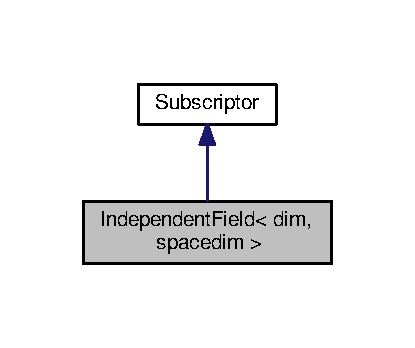
\includegraphics[width=213pt]{class_independent_field__inherit__graph}
\end{center}
\end{figure}


Collaboration diagram for Independent\+Field$<$ dim, spacedim $>$\+:\nopagebreak
\begin{figure}[H]
\begin{center}
\leavevmode
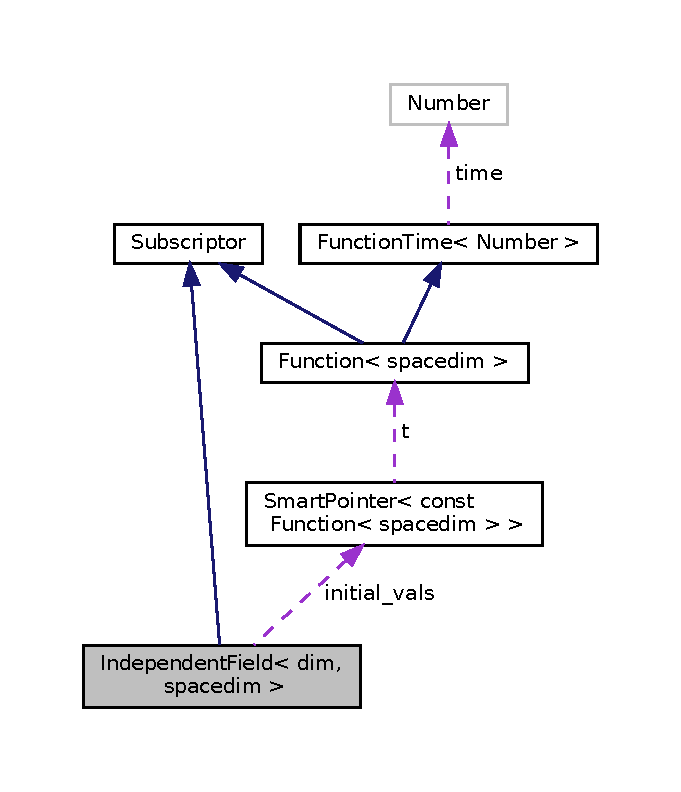
\includegraphics[width=327pt]{class_independent_field__coll__graph}
\end{center}
\end{figure}
\doxysubsection*{Public Member Functions}
\begin{DoxyCompactItemize}
\item 
\mbox{\hyperlink{class_independent_field_afb12ec32511568a9504312730542bfa1}{Independent\+Field}} (const std\+::string \mbox{\hyperlink{class_independent_field_ae05f8565e4ce1a70b5b833555dc084b5}{name}}, const \textbf{ Finite\+Element}$<$ dim, spacedim $>$ \&\mbox{\hyperlink{class_independent_field_a1c583665b7710bd3b815b03ba026b6d3}{fe}}, const unsigned int \mbox{\hyperlink{class_independent_field_a7b19ea8c30d72cf27f05669de61f30a8}{n\+\_\+components}}, const std\+::set$<$ \textbf{ types\+::material\+\_\+id} $>$ \mbox{\hyperlink{class_independent_field_a4e09e114870c0b3761bc2e32916e5850}{non\+\_\+zero\+\_\+regions}}, const \textbf{ Function}$<$ spacedim $>$ $\ast$const \mbox{\hyperlink{class_independent_field_a274c902785d2937a6065f7e09f3976c3}{initial\+\_\+vals}}=nullptr, const bool \mbox{\hyperlink{class_independent_field_a8e77d8d321a259bec955a71f55ef41e5}{is\+\_\+local}}=false, const bool \mbox{\hyperlink{class_independent_field_a755514cb31014d9b39e1b3e677c4527d}{is\+\_\+locally\+\_\+eliminated}}=false)
\item 
\mbox{\hyperlink{class_independent_field_af953c9ecc5965d5bcbd61fab9e0b6e2b}{Independent\+Field}} (const std\+::string \mbox{\hyperlink{class_independent_field_ae05f8565e4ce1a70b5b833555dc084b5}{name}}, const \textbf{ Finite\+Element}$<$ dim, spacedim $>$ \&\mbox{\hyperlink{class_independent_field_a1c583665b7710bd3b815b03ba026b6d3}{fe}}, const std\+::set$<$ \textbf{ types\+::material\+\_\+id} $>$ \mbox{\hyperlink{class_independent_field_a4e09e114870c0b3761bc2e32916e5850}{non\+\_\+zero\+\_\+regions}}, const \textbf{ Function}$<$ spacedim $>$ $\ast$const \mbox{\hyperlink{class_independent_field_a274c902785d2937a6065f7e09f3976c3}{initial\+\_\+vals}}=nullptr)
\item 
\mbox{\hyperlink{class_independent_field_af83ee8c1600bb079a3075244a7b39481}{$\sim$\+Independent\+Field}} ()
\end{DoxyCompactItemize}
\doxysubsection*{Public Attributes}
\begin{DoxyCompactItemize}
\item 
const std\+::string \mbox{\hyperlink{class_independent_field_ae05f8565e4ce1a70b5b833555dc084b5}{name}}
\item 
const std\+::unique\+\_\+ptr$<$ const \textbf{ Finite\+Element}$<$ dim, spacedim $>$ $>$ \mbox{\hyperlink{class_independent_field_a1c583665b7710bd3b815b03ba026b6d3}{fe}}
\item 
const unsigned int \mbox{\hyperlink{class_independent_field_a7b19ea8c30d72cf27f05669de61f30a8}{n\+\_\+components}}
\item 
const std\+::set$<$ \textbf{ types\+::material\+\_\+id} $>$ \mbox{\hyperlink{class_independent_field_a4e09e114870c0b3761bc2e32916e5850}{non\+\_\+zero\+\_\+regions}}
\item 
const \textbf{ Smart\+Pointer}$<$ const \textbf{ Function}$<$ spacedim $>$ $>$ \mbox{\hyperlink{class_independent_field_a274c902785d2937a6065f7e09f3976c3}{initial\+\_\+vals}}
\item 
const bool \mbox{\hyperlink{class_independent_field_a8e77d8d321a259bec955a71f55ef41e5}{is\+\_\+local}} = false
\item 
const bool \mbox{\hyperlink{class_independent_field_a755514cb31014d9b39e1b3e677c4527d}{is\+\_\+locally\+\_\+eliminated}} = false
\end{DoxyCompactItemize}
\doxysubsection*{Additional Inherited Members}


\doxysubsection{Detailed Description}
\subsubsection*{template$<$unsigned int dim, unsigned int spacedim$>$\newline
class Independent\+Field$<$ dim, spacedim $>$}

This class is used to define \char`\"{}independent fields\char`\"{}, which are the unknowns of the problem to be solved. Currently domain related and interface related fields are considered, which live on the domain $\Omega$ and the interface $\Sigma$, respectively.

Domain related fields are denoted by $u^\Omega_\epsilon(\boldsymbol{X})$, where $\epsilon \in E=\left\{1 \hdots N^\mathrm{u,\Omega}\right\}$ enumerates the independent fields, and $\boldsymbol{X} \in \mathcal{R}^n$ is the location in Euclidean $n$-\/space.

Interface related fields are denoted by $u^\Sigma_\eta(\boldsymbol{X})$, where $\eta \in H=\left\{1 \hdots N^\mathrm{u,\Sigma}\right\}$.

Each $u^\Omega_\epsilon$ and $u^\Sigma_\eta$, respectively, is considered a scalar valued field. \textbf{ Vector} and tensor valued independent fields may be represented by combining several scalar valued fields.

In order to allow for the use of vector valued finite elements, each \mbox{\hyperlink{class_independent_field}{Independent\+Field}} object may represent a $K$-\/vector of scalar valued independent fields. The restriction is, however, that either all $K$ vector components are discretized with the same (scalar valued) finite element, or that the complete $K$-\/vector is discretized by a single (vector valued) finite element.

The \mbox{\hyperlink{class_independent_field}{Independent\+Field}} class inherits from \textbf{ Subscriptor} in order to be able to check that \mbox{\hyperlink{class_independent_field}{Independent\+Field}} objects are only destroyed when they are not needed anymore by other objects.


\begin{DoxyTemplParams}{Template Parameters}
{\em spacedim} & This template parameter represents the spatial dimension $n$ of the space wherein the problem is formulated.\\
\hline
{\em dim} & This template parameter represents the dimensionality of the object on which the $K$-\/vector of independent fields represented by the \mbox{\hyperlink{class_independent_field}{Independent\+Field}} object lives. E.\+g., an \mbox{\hyperlink{class_independent_field}{Independent\+Field}} $<$3,3$>$ represents a field living on the domain in Euclidean $3$-\/space, while an \mbox{\hyperlink{class_independent_field}{Independent\+Field}} $<$2,3$>$ represents a field living on an interface or boundary embedded in Euclidean $3$-\/space. \\
\hline
\end{DoxyTemplParams}


\doxysubsection{Constructor \& Destructor Documentation}
\mbox{\Hypertarget{class_independent_field_afb12ec32511568a9504312730542bfa1}\label{class_independent_field_afb12ec32511568a9504312730542bfa1}} 
\index{IndependentField$<$ dim, spacedim $>$@{IndependentField$<$ dim, spacedim $>$}!IndependentField@{IndependentField}}
\index{IndependentField@{IndependentField}!IndependentField$<$ dim, spacedim $>$@{IndependentField$<$ dim, spacedim $>$}}
\doxysubsubsection{\texorpdfstring{IndependentField()}{IndependentField()}\hspace{0.1cm}{\footnotesize\ttfamily [1/2]}}
{\footnotesize\ttfamily template$<$unsigned int dim, unsigned int spacedim$>$ \\
\mbox{\hyperlink{class_independent_field}{Independent\+Field}}$<$ dim, spacedim $>$\+::\mbox{\hyperlink{class_independent_field}{Independent\+Field}} (\begin{DoxyParamCaption}\item[{const std\+::string}]{name,  }\item[{const \textbf{ Finite\+Element}$<$ dim, spacedim $>$ \&}]{fe,  }\item[{const unsigned int}]{n\+\_\+components,  }\item[{const std\+::set$<$ \textbf{ types\+::material\+\_\+id} $>$}]{non\+\_\+zero\+\_\+regions,  }\item[{const \textbf{ Function}$<$ spacedim $>$ $\ast$const}]{initial\+\_\+vals = {\ttfamily nullptr},  }\item[{const bool}]{is\+\_\+local = {\ttfamily false},  }\item[{const bool}]{is\+\_\+locally\+\_\+eliminated = {\ttfamily false} }\end{DoxyParamCaption})}

The constructor of the class for the case that \mbox{\hyperlink{class_independent_field_a7b19ea8c30d72cf27f05669de61f30a8}{Independent\+Field\+::n\+\_\+components}} copies of a scalar valued finite element are used for discretization of the $K$-\/vector of independent fields represented by the \mbox{\hyperlink{class_independent_field}{Independent\+Field}} object.


\begin{DoxyParams}[1]{Parameters}
\mbox{\texttt{ in}}  & {\em name} & \mbox{\hyperlink{class_independent_field_ae05f8565e4ce1a70b5b833555dc084b5}{Independent\+Field\+::name}}\\
\hline
\mbox{\texttt{ in}}  & {\em fe} & \mbox{\hyperlink{class_independent_field_a1c583665b7710bd3b815b03ba026b6d3}{Independent\+Field\+::fe}}, must be a scalar valued finite element\\
\hline
\mbox{\texttt{ in}}  & {\em n\+\_\+components} & \mbox{\hyperlink{class_independent_field_a7b19ea8c30d72cf27f05669de61f30a8}{Independent\+Field\+::n\+\_\+components}}\\
\hline
\mbox{\texttt{ in}}  & {\em non\+\_\+zero\+\_\+regions} & \mbox{\hyperlink{class_independent_field_a4e09e114870c0b3761bc2e32916e5850}{Independent\+Field\+::non\+\_\+zero\+\_\+regions}}\\
\hline
\mbox{\texttt{ in}}  & {\em initial\+\_\+vals} & \mbox{\hyperlink{class_independent_field_a274c902785d2937a6065f7e09f3976c3}{Independent\+Field\+::initial\+\_\+vals}}, if a null pointer is provided, the initial values of the independent fields are assumed to be zero.\\
\hline
\mbox{\texttt{ in}}  & {\em is\+\_\+local} & \mbox{\hyperlink{class_independent_field_a8e77d8d321a259bec955a71f55ef41e5}{Independent\+Field\+::is\+\_\+local}}\\
\hline
\mbox{\texttt{ in}}  & {\em is\+\_\+locally\+\_\+eliminated} & \mbox{\hyperlink{class_independent_field_a755514cb31014d9b39e1b3e677c4527d}{Independent\+Field\+::is\+\_\+locally\+\_\+eliminated}} \\
\hline
\end{DoxyParams}
\mbox{\Hypertarget{class_independent_field_af953c9ecc5965d5bcbd61fab9e0b6e2b}\label{class_independent_field_af953c9ecc5965d5bcbd61fab9e0b6e2b}} 
\index{IndependentField$<$ dim, spacedim $>$@{IndependentField$<$ dim, spacedim $>$}!IndependentField@{IndependentField}}
\index{IndependentField@{IndependentField}!IndependentField$<$ dim, spacedim $>$@{IndependentField$<$ dim, spacedim $>$}}
\doxysubsubsection{\texorpdfstring{IndependentField()}{IndependentField()}\hspace{0.1cm}{\footnotesize\ttfamily [2/2]}}
{\footnotesize\ttfamily template$<$unsigned int dim, unsigned int spacedim$>$ \\
\mbox{\hyperlink{class_independent_field}{Independent\+Field}}$<$ dim, spacedim $>$\+::\mbox{\hyperlink{class_independent_field}{Independent\+Field}} (\begin{DoxyParamCaption}\item[{const std\+::string}]{name,  }\item[{const \textbf{ Finite\+Element}$<$ dim, spacedim $>$ \&}]{fe,  }\item[{const std\+::set$<$ \textbf{ types\+::material\+\_\+id} $>$}]{non\+\_\+zero\+\_\+regions,  }\item[{const \textbf{ Function}$<$ spacedim $>$ $\ast$const}]{initial\+\_\+vals = {\ttfamily nullptr} }\end{DoxyParamCaption})}

The constructor of the class for the case that a vector valued finite element is used for discretization of the $K$-\/vector of independent fields represented by the \mbox{\hyperlink{class_independent_field}{Independent\+Field}} object. With this constructor, \mbox{\hyperlink{class_independent_field_a7b19ea8c30d72cf27f05669de61f30a8}{Independent\+Field\+::n\+\_\+components}} will be deduced from the number of components of the \mbox{\hyperlink{class_independent_field_a1c583665b7710bd3b815b03ba026b6d3}{Independent\+Field\+::fe}} object.


\begin{DoxyParams}[1]{Parameters}
\mbox{\texttt{ in}}  & {\em name} & \mbox{\hyperlink{class_independent_field_ae05f8565e4ce1a70b5b833555dc084b5}{Independent\+Field\+::name}}\\
\hline
\mbox{\texttt{ in}}  & {\em fe} & \mbox{\hyperlink{class_independent_field_a1c583665b7710bd3b815b03ba026b6d3}{Independent\+Field\+::fe}}\\
\hline
\mbox{\texttt{ in}}  & {\em non\+\_\+zero\+\_\+regions} & \mbox{\hyperlink{class_independent_field_a4e09e114870c0b3761bc2e32916e5850}{Independent\+Field\+::non\+\_\+zero\+\_\+regions}}\\
\hline
\mbox{\texttt{ in}}  & {\em initial\+\_\+vals} & \mbox{\hyperlink{class_independent_field_a274c902785d2937a6065f7e09f3976c3}{Independent\+Field\+::initial\+\_\+vals}}, if a null pointer is provided, the initial values of the independent fields are assumed to be zero. \\
\hline
\end{DoxyParams}
\mbox{\Hypertarget{class_independent_field_af83ee8c1600bb079a3075244a7b39481}\label{class_independent_field_af83ee8c1600bb079a3075244a7b39481}} 
\index{IndependentField$<$ dim, spacedim $>$@{IndependentField$<$ dim, spacedim $>$}!````~IndependentField@{$\sim$IndependentField}}
\index{````~IndependentField@{$\sim$IndependentField}!IndependentField$<$ dim, spacedim $>$@{IndependentField$<$ dim, spacedim $>$}}
\doxysubsubsection{\texorpdfstring{$\sim$IndependentField()}{~IndependentField()}}
{\footnotesize\ttfamily template$<$unsigned int dim, unsigned int spacedim$>$ \\
\mbox{\hyperlink{class_independent_field}{Independent\+Field}}$<$ dim, spacedim $>$\+::$\sim$\mbox{\hyperlink{class_independent_field}{Independent\+Field}} (\begin{DoxyParamCaption}{ }\end{DoxyParamCaption})}

The destructor of \mbox{\hyperlink{class_independent_field}{Independent\+Field}} essentially checks before destruction that the \mbox{\hyperlink{class_independent_field}{Independent\+Field}} object is not used by other objects. If this is the case, the program will be aborted. 

\doxysubsection{Member Data Documentation}
\mbox{\Hypertarget{class_independent_field_a1c583665b7710bd3b815b03ba026b6d3}\label{class_independent_field_a1c583665b7710bd3b815b03ba026b6d3}} 
\index{IndependentField$<$ dim, spacedim $>$@{IndependentField$<$ dim, spacedim $>$}!fe@{fe}}
\index{fe@{fe}!IndependentField$<$ dim, spacedim $>$@{IndependentField$<$ dim, spacedim $>$}}
\doxysubsubsection{\texorpdfstring{fe}{fe}}
{\footnotesize\ttfamily template$<$unsigned int dim, unsigned int spacedim$>$ \\
const std\+::unique\+\_\+ptr$<$const \textbf{ Finite\+Element}$<$dim, spacedim$>$ $>$ \mbox{\hyperlink{class_independent_field}{Independent\+Field}}$<$ dim, spacedim $>$\+::fe}

The finite element used for the discretization of the $K$-\/vector of independent fields represented by the \mbox{\hyperlink{class_independent_field}{Independent\+Field}} object. The finite element stored here may be either scalar valued (in which case \mbox{\hyperlink{class_independent_field_a7b19ea8c30d72cf27f05669de61f30a8}{Independent\+Field\+::n\+\_\+components}} copies of \mbox{\hyperlink{class_independent_field_a1c583665b7710bd3b815b03ba026b6d3}{Independent\+Field\+::fe}} are used to discretize all the vector components) or vector valued (in which case its number of components must equal \mbox{\hyperlink{class_independent_field_a7b19ea8c30d72cf27f05669de61f30a8}{Independent\+Field\+::n\+\_\+components}}). \mbox{\Hypertarget{class_independent_field_a274c902785d2937a6065f7e09f3976c3}\label{class_independent_field_a274c902785d2937a6065f7e09f3976c3}} 
\index{IndependentField$<$ dim, spacedim $>$@{IndependentField$<$ dim, spacedim $>$}!initial\_vals@{initial\_vals}}
\index{initial\_vals@{initial\_vals}!IndependentField$<$ dim, spacedim $>$@{IndependentField$<$ dim, spacedim $>$}}
\doxysubsubsection{\texorpdfstring{initial\_vals}{initial\_vals}}
{\footnotesize\ttfamily template$<$unsigned int dim, unsigned int spacedim$>$ \\
const \textbf{ Smart\+Pointer}$<$const \textbf{ Function}$<$spacedim$>$ $>$ \mbox{\hyperlink{class_independent_field}{Independent\+Field}}$<$ dim, spacedim $>$\+::initial\+\_\+vals}

A \textbf{ Function} (or, rather, an instance of a derived class) specifying the initial values of the independent fields represented by \mbox{\hyperlink{class_independent_field}{Independent\+Field}} as a function of position in space. The \textbf{ Function} must implement the method \textbf{ Function\+::value()}, which provides with the initial values for all \mbox{\hyperlink{class_independent_field_a7b19ea8c30d72cf27f05669de61f30a8}{Independent\+Field\+::n\+\_\+components}} components. \mbox{\Hypertarget{class_independent_field_a8e77d8d321a259bec955a71f55ef41e5}\label{class_independent_field_a8e77d8d321a259bec955a71f55ef41e5}} 
\index{IndependentField$<$ dim, spacedim $>$@{IndependentField$<$ dim, spacedim $>$}!is\_local@{is\_local}}
\index{is\_local@{is\_local}!IndependentField$<$ dim, spacedim $>$@{IndependentField$<$ dim, spacedim $>$}}
\doxysubsubsection{\texorpdfstring{is\_local}{is\_local}}
{\footnotesize\ttfamily template$<$unsigned int dim, unsigned int spacedim$>$ \\
const bool \mbox{\hyperlink{class_independent_field}{Independent\+Field}}$<$ dim, spacedim $>$\+::is\+\_\+local = false}

If this is true, the independent field is assumed to be local. In this case, the following restrictions apply\+:


\begin{DoxyItemize}
\item The independent field must be discretized by an \textbf{ F\+E\+\_\+\+D\+G\+Q\+Arbitrary\+Nodes} of deal.\+II.
\item The quadrature points used for the integration process of the scalar functionals involving the independent field must coincide with the support points of the used \textbf{ F\+E\+\_\+\+D\+G\+Q\+Arbitrary\+Nodes}.
\item All scalar functionals involving the independent field must be primitive.
\item The independent field must not be associated with constraints. \begin{DoxyRefDesc}{Todo}
\item[\mbox{\hyperlink{todo__todo000012}{Todo}}]The latter may be relaxed to a certain degree. This needs, however, to be implemented.\end{DoxyRefDesc}

\end{DoxyItemize}

The effect of setting this to true is that the entries in the sparsity pattern can be substantially reduced. \mbox{\Hypertarget{class_independent_field_a755514cb31014d9b39e1b3e677c4527d}\label{class_independent_field_a755514cb31014d9b39e1b3e677c4527d}} 
\index{IndependentField$<$ dim, spacedim $>$@{IndependentField$<$ dim, spacedim $>$}!is\_locally\_eliminated@{is\_locally\_eliminated}}
\index{is\_locally\_eliminated@{is\_locally\_eliminated}!IndependentField$<$ dim, spacedim $>$@{IndependentField$<$ dim, spacedim $>$}}
\doxysubsubsection{\texorpdfstring{is\_locally\_eliminated}{is\_locally\_eliminated}}
{\footnotesize\ttfamily template$<$unsigned int dim, unsigned int spacedim$>$ \\
const bool \mbox{\hyperlink{class_independent_field}{Independent\+Field}}$<$ dim, spacedim $>$\+::is\+\_\+locally\+\_\+eliminated = false}

If this is true, the independent field is assumed to be locally eliminated at the quadrature point level in that the local value of the independent field can be determined at the quadrature point level based on the previous local values of the independent field and the current and previous local values of the other field variables.

Note also that this can only be true if \mbox{\hyperlink{class_independent_field_a8e77d8d321a259bec955a71f55ef41e5}{Independent\+Field\+::is\+\_\+local}} is true as well and, therefore, the restrictions for local fields apply. However, in addition it is necessary that the scalar functional locally determines the new values of the independent field. In order to implement a simple mechanism for feeding these new values back to the global assembly scheme, it is additionally assumed that the locally eliminated independent fields have a 1 to 1 correspondence to a dependent field in that the dependent field equals the independent field. Thus, the mechanism for feeding the new values back is simply that the scalar functional updates the respective value of the dependent field associated with the locally eliminated independent field.

The purpose of the mechanism just described is that \char`\"{}hidden/internal\char`\"{} variables, which are common in continuum mechanics, can be easily incorporated without the need of additional data structures storing them. \mbox{\Hypertarget{class_independent_field_a7b19ea8c30d72cf27f05669de61f30a8}\label{class_independent_field_a7b19ea8c30d72cf27f05669de61f30a8}} 
\index{IndependentField$<$ dim, spacedim $>$@{IndependentField$<$ dim, spacedim $>$}!n\_components@{n\_components}}
\index{n\_components@{n\_components}!IndependentField$<$ dim, spacedim $>$@{IndependentField$<$ dim, spacedim $>$}}
\doxysubsubsection{\texorpdfstring{n\_components}{n\_components}}
{\footnotesize\ttfamily template$<$unsigned int dim, unsigned int spacedim$>$ \\
const unsigned int \mbox{\hyperlink{class_independent_field}{Independent\+Field}}$<$ dim, spacedim $>$\+::n\+\_\+components}

The number of vector components associated with the \mbox{\hyperlink{class_independent_field}{Independent\+Field}} object. In case that the finite element \mbox{\hyperlink{class_independent_field_a1c583665b7710bd3b815b03ba026b6d3}{Independent\+Field\+::fe}} is scalar valued, \mbox{\hyperlink{class_independent_field_a7b19ea8c30d72cf27f05669de61f30a8}{Independent\+Field\+::n\+\_\+components}} corresponds to the multiplicity of the finite element. In case that the finite element \mbox{\hyperlink{class_independent_field_a1c583665b7710bd3b815b03ba026b6d3}{Independent\+Field\+::fe}} is vector valued, the number of components of \mbox{\hyperlink{class_independent_field_a1c583665b7710bd3b815b03ba026b6d3}{Independent\+Field\+::fe}} must correspond to \mbox{\hyperlink{class_independent_field_a7b19ea8c30d72cf27f05669de61f30a8}{Independent\+Field\+::n\+\_\+components}}. \mbox{\Hypertarget{class_independent_field_ae05f8565e4ce1a70b5b833555dc084b5}\label{class_independent_field_ae05f8565e4ce1a70b5b833555dc084b5}} 
\index{IndependentField$<$ dim, spacedim $>$@{IndependentField$<$ dim, spacedim $>$}!name@{name}}
\index{name@{name}!IndependentField$<$ dim, spacedim $>$@{IndependentField$<$ dim, spacedim $>$}}
\doxysubsubsection{\texorpdfstring{name}{name}}
{\footnotesize\ttfamily template$<$unsigned int dim, unsigned int spacedim$>$ \\
const std\+::string \mbox{\hyperlink{class_independent_field}{Independent\+Field}}$<$ dim, spacedim $>$\+::name}

A string with a unique name for the \mbox{\hyperlink{class_independent_field}{Independent\+Field}} object, which is used to identify it in output and to ensure a well defined ordering of \mbox{\hyperlink{class_independent_field}{Independent\+Field}} objects. \mbox{\Hypertarget{class_independent_field_a4e09e114870c0b3761bc2e32916e5850}\label{class_independent_field_a4e09e114870c0b3761bc2e32916e5850}} 
\index{IndependentField$<$ dim, spacedim $>$@{IndependentField$<$ dim, spacedim $>$}!non\_zero\_regions@{non\_zero\_regions}}
\index{non\_zero\_regions@{non\_zero\_regions}!IndependentField$<$ dim, spacedim $>$@{IndependentField$<$ dim, spacedim $>$}}
\doxysubsubsection{\texorpdfstring{non\_zero\_regions}{non\_zero\_regions}}
{\footnotesize\ttfamily template$<$unsigned int dim, unsigned int spacedim$>$ \\
const std\+::set$<$\textbf{ types\+::material\+\_\+id}$>$ \mbox{\hyperlink{class_independent_field}{Independent\+Field}}$<$ dim, spacedim $>$\+::non\+\_\+zero\+\_\+regions}

A set of \textbf{ types\+::material\+\_\+id} indicating on which domain/interface portions the independent fields represented by the \mbox{\hyperlink{class_independent_field}{Independent\+Field}} object are non-\/zero. On all cells of the triangulation having a \textbf{ types\+::material\+\_\+id} listed in \mbox{\hyperlink{class_independent_field_a4e09e114870c0b3761bc2e32916e5850}{Independent\+Field\+::non\+\_\+zero\+\_\+regions}}, the finite element \mbox{\hyperlink{class_independent_field_a1c583665b7710bd3b815b03ba026b6d3}{Independent\+Field\+::fe}} will be used for discretization. In contrast, on a cell with a material id not listed in \mbox{\hyperlink{class_independent_field_a4e09e114870c0b3761bc2e32916e5850}{Independent\+Field\+::non\+\_\+zero\+\_\+regions}}, the independent fields are assumed to be zero and are \char`\"{}discretized\char`\"{} by \mbox{\hyperlink{class_independent_field_a7b19ea8c30d72cf27f05669de61f30a8}{Independent\+Field\+::n\+\_\+components}} copies of \textbf{ F\+E\+\_\+\+Nothing}. 

The documentation for this class was generated from the following file\+:\begin{DoxyCompactItemize}
\item 
/home/sst/code/\+Galerkin\+Tools/\+Galerkin\+Tools/include/galerkin\+\_\+tools/\mbox{\hyperlink{independent__field_8h}{independent\+\_\+field.\+h}}\end{DoxyCompactItemize}

\hypertarget{class_independent_field_3_010_00_01spacedim_01_4}{}\section{Independent\+Field$<$ 0, spacedim $>$ Class Template Reference}
\label{class_independent_field_3_010_00_01spacedim_01_4}\index{Independent\+Field$<$ 0, spacedim $>$@{Independent\+Field$<$ 0, spacedim $>$}}


{\ttfamily \#include $<$independent\+\_\+field.\+h$>$}



Inheritance diagram for Independent\+Field$<$ 0, spacedim $>$\+:
\nopagebreak
\begin{figure}[H]
\begin{center}
\leavevmode
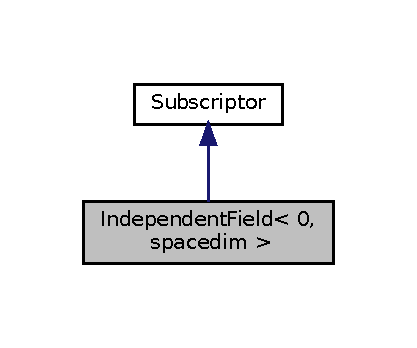
\includegraphics[width=188pt]{class_independent_field_3_010_00_01spacedim_01_4__inherit__graph}
\end{center}
\end{figure}


Collaboration diagram for Independent\+Field$<$ 0, spacedim $>$\+:
\nopagebreak
\begin{figure}[H]
\begin{center}
\leavevmode
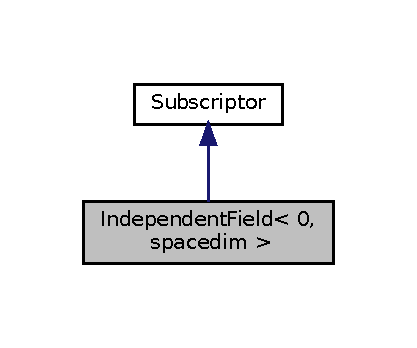
\includegraphics[width=188pt]{class_independent_field_3_010_00_01spacedim_01_4__coll__graph}
\end{center}
\end{figure}
\subsection*{Public Member Functions}
\begin{DoxyCompactItemize}
\item 
\hyperlink{class_independent_field_3_010_00_01spacedim_01_4_a8a486862088446941ea97fc471c5d44c}{Independent\+Field} (const std\+::string \hyperlink{class_independent_field_3_010_00_01spacedim_01_4_a05ecdcc8310253f055fbc59abaa2bc90}{name}, const double \hyperlink{class_independent_field_3_010_00_01spacedim_01_4_a8c4c434806dadc5b885102322e27357c}{initial\+\_\+value}=0.\+0)
\item 
\hyperlink{class_independent_field_3_010_00_01spacedim_01_4_a653c01f2a6aeffba44542d9788433647}{$\sim$\+Independent\+Field} ()
\end{DoxyCompactItemize}
\subsection*{Public Attributes}
\begin{DoxyCompactItemize}
\item 
const std\+::string \hyperlink{class_independent_field_3_010_00_01spacedim_01_4_a05ecdcc8310253f055fbc59abaa2bc90}{name}
\item 
const double \hyperlink{class_independent_field_3_010_00_01spacedim_01_4_a8c4c434806dadc5b885102322e27357c}{initial\+\_\+value}
\item 
const unsigned int \hyperlink{class_independent_field_3_010_00_01spacedim_01_4_a248c2226570c71914f5219e7e3052561}{n\+\_\+components} = 1
\end{DoxyCompactItemize}
\subsection*{Additional Inherited Members}


\subsection{Detailed Description}
\subsubsection*{template$<$unsigned int spacedim$>$\\*
class Independent\+Field$<$ 0, spacedim $>$}

This class is used to define an independent scalar $C_\iota$, where $\iota \in I=\left\{1 \hdots N^\mathrm{C}\right\}$ enumerates the independent scalars (which may be interpreted as independent fields living on a single point in space). 

\subsection{Constructor \& Destructor Documentation}
\index{Independent\+Field$<$ 0, spacedim $>$@{Independent\+Field$<$ 0, spacedim $>$}!Independent\+Field@{Independent\+Field}}
\index{Independent\+Field@{Independent\+Field}!Independent\+Field$<$ 0, spacedim $>$@{Independent\+Field$<$ 0, spacedim $>$}}
\subsubsection[{\texorpdfstring{Independent\+Field(const std\+::string name, const double initial\+\_\+value=0.\+0)}{IndependentField(const std::string name, const double initial_value=0.0)}}]{\setlength{\rightskip}{0pt plus 5cm}template$<$unsigned int spacedim$>$ {\bf Independent\+Field}$<$ 0, spacedim $>$\+::{\bf Independent\+Field} (
\begin{DoxyParamCaption}
\item[{const std\+::string}]{name, }
\item[{const double}]{initial\+\_\+value = {\ttfamily 0.0}}
\end{DoxyParamCaption}
)}\hypertarget{class_independent_field_3_010_00_01spacedim_01_4_a8a486862088446941ea97fc471c5d44c}{}\label{class_independent_field_3_010_00_01spacedim_01_4_a8a486862088446941ea97fc471c5d44c}
The constructor of the class.


\begin{DoxyParams}[1]{Parameters}
\mbox{\tt in}  & {\em name} & \hyperlink{class_independent_field_3_010_00_01spacedim_01_4_a05ecdcc8310253f055fbc59abaa2bc90}{Independent\+Field$<$0, spacedim$>$\+::name}\\
\hline
\mbox{\tt in}  & {\em initial\+\_\+value} & \hyperlink{class_independent_field_3_010_00_01spacedim_01_4_a8c4c434806dadc5b885102322e27357c}{Independent\+Field$<$0, spacedim$>$\+::initial\+\_\+value} \\
\hline
\end{DoxyParams}
\index{Independent\+Field$<$ 0, spacedim $>$@{Independent\+Field$<$ 0, spacedim $>$}!````~Independent\+Field@{$\sim$\+Independent\+Field}}
\index{````~Independent\+Field@{$\sim$\+Independent\+Field}!Independent\+Field$<$ 0, spacedim $>$@{Independent\+Field$<$ 0, spacedim $>$}}
\subsubsection[{\texorpdfstring{$\sim$\+Independent\+Field()}{~IndependentField()}}]{\setlength{\rightskip}{0pt plus 5cm}template$<$unsigned int spacedim$>$ {\bf Independent\+Field}$<$ 0, spacedim $>$\+::$\sim${\bf Independent\+Field} (
\begin{DoxyParamCaption}
{}
\end{DoxyParamCaption}
)}\hypertarget{class_independent_field_3_010_00_01spacedim_01_4_a653c01f2a6aeffba44542d9788433647}{}\label{class_independent_field_3_010_00_01spacedim_01_4_a653c01f2a6aeffba44542d9788433647}
The destructor of \hyperlink{class_independent_field_3_010_00_01spacedim_01_4}{Independent\+Field$<$0, spacedim$>$} essentially checks before destruction that the \hyperlink{class_independent_field_3_010_00_01spacedim_01_4}{Independent\+Field$<$0, spacedim$>$} object is not used by other objects. If this is the case, the program will be aborted. 

\subsection{Member Data Documentation}
\index{Independent\+Field$<$ 0, spacedim $>$@{Independent\+Field$<$ 0, spacedim $>$}!initial\+\_\+value@{initial\+\_\+value}}
\index{initial\+\_\+value@{initial\+\_\+value}!Independent\+Field$<$ 0, spacedim $>$@{Independent\+Field$<$ 0, spacedim $>$}}
\subsubsection[{\texorpdfstring{initial\+\_\+value}{initial_value}}]{\setlength{\rightskip}{0pt plus 5cm}template$<$unsigned int spacedim$>$ const double {\bf Independent\+Field}$<$ 0, spacedim $>$\+::initial\+\_\+value}\hypertarget{class_independent_field_3_010_00_01spacedim_01_4_a8c4c434806dadc5b885102322e27357c}{}\label{class_independent_field_3_010_00_01spacedim_01_4_a8c4c434806dadc5b885102322e27357c}
The initial value of the independent field. \index{Independent\+Field$<$ 0, spacedim $>$@{Independent\+Field$<$ 0, spacedim $>$}!n\+\_\+components@{n\+\_\+components}}
\index{n\+\_\+components@{n\+\_\+components}!Independent\+Field$<$ 0, spacedim $>$@{Independent\+Field$<$ 0, spacedim $>$}}
\subsubsection[{\texorpdfstring{n\+\_\+components}{n_components}}]{\setlength{\rightskip}{0pt plus 5cm}template$<$unsigned int spacedim$>$ const unsigned int {\bf Independent\+Field}$<$ 0, spacedim $>$\+::n\+\_\+components = 1}\hypertarget{class_independent_field_3_010_00_01spacedim_01_4_a248c2226570c71914f5219e7e3052561}{}\label{class_independent_field_3_010_00_01spacedim_01_4_a248c2226570c71914f5219e7e3052561}
The number of vector components associated with the \hyperlink{class_independent_field_3_010_00_01spacedim_01_4}{Independent\+Field$<$0, spacedim$>$} object. Here, only \hyperlink{class_independent_field_3_010_00_01spacedim_01_4_a248c2226570c71914f5219e7e3052561}{Independent\+Field$<$0, spacedim$>$\+::n\+\_\+components} = 1 is allowed, because no vector valued independent scalars are considered at present (although they may be represented by several \hyperlink{class_independent_field_3_010_00_01spacedim_01_4}{Independent\+Field$<$0, spacedim$>$} objects). \index{Independent\+Field$<$ 0, spacedim $>$@{Independent\+Field$<$ 0, spacedim $>$}!name@{name}}
\index{name@{name}!Independent\+Field$<$ 0, spacedim $>$@{Independent\+Field$<$ 0, spacedim $>$}}
\subsubsection[{\texorpdfstring{name}{name}}]{\setlength{\rightskip}{0pt plus 5cm}template$<$unsigned int spacedim$>$ const std\+::string {\bf Independent\+Field}$<$ 0, spacedim $>$\+::name}\hypertarget{class_independent_field_3_010_00_01spacedim_01_4_a05ecdcc8310253f055fbc59abaa2bc90}{}\label{class_independent_field_3_010_00_01spacedim_01_4_a05ecdcc8310253f055fbc59abaa2bc90}
A string with a unique name for the \hyperlink{class_independent_field_3_010_00_01spacedim_01_4}{Independent\+Field$<$0, spacedim$>$} object, which is used to identify it in output and to ensure a well defined ordering of \hyperlink{class_independent_field_3_010_00_01spacedim_01_4}{Independent\+Field$<$0, spacedim$>$} objects. 

The documentation for this class was generated from the following file\+:\begin{DoxyCompactItemize}
\item 
/home/sst/code/\+Galerkin\+Tools/\+Galerkin\+Tools/include/galerkin\+\_\+tools/\hyperlink{independent__field_8h}{independent\+\_\+field.\+h}\end{DoxyCompactItemize}

\hypertarget{class_interface_cell_do_f_iterator}{}\doxysection{Interface\+Cell\+Do\+F\+Iterator$<$ spacedim $>$ Class Template Reference}
\label{class_interface_cell_do_f_iterator}\index{InterfaceCellDoFIterator$<$ spacedim $>$@{InterfaceCellDoFIterator$<$ spacedim $>$}}


{\ttfamily \#include $<$dof\+\_\+handler\+\_\+system.\+h$>$}



Inheritance diagram for Interface\+Cell\+Do\+F\+Iterator$<$ spacedim $>$\+:\nopagebreak
\begin{figure}[H]
\begin{center}
\leavevmode
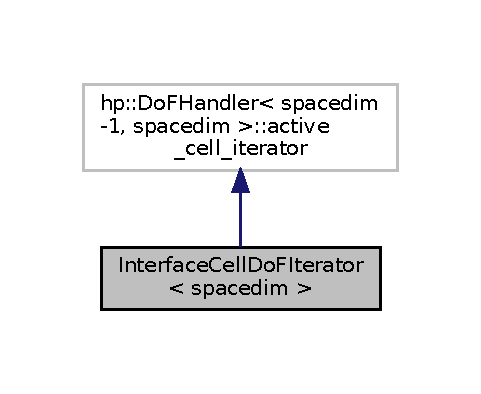
\includegraphics[width=231pt]{class_interface_cell_do_f_iterator__inherit__graph}
\end{center}
\end{figure}


Collaboration diagram for Interface\+Cell\+Do\+F\+Iterator$<$ spacedim $>$\+:\nopagebreak
\begin{figure}[H]
\begin{center}
\leavevmode
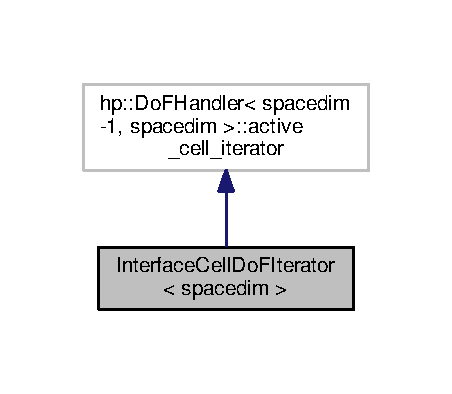
\includegraphics[width=231pt]{class_interface_cell_do_f_iterator__coll__graph}
\end{center}
\end{figure}
\doxysubsection*{Public Member Functions}
\begin{DoxyCompactItemize}
\item 
\mbox{\hyperlink{class_interface_cell_do_f_iterator_a41a74a50c801c67a5393d568ed2768b7}{Interface\+Cell\+Do\+F\+Iterator}} (const \textbf{ Tria\+Iterator}$<$ \textbf{ Cell\+Accessor}$<$ spacedim-\/1, spacedim $>$$>$ \&interface\+\_\+cell, const \mbox{\hyperlink{class_do_f_handler_system}{Do\+F\+Handler\+System}}$<$ spacedim $>$ \&\mbox{\hyperlink{class_interface_cell_do_f_iterator_a62045b61faee901392a7326b624d2b02}{dof\+\_\+handler\+\_\+system}})
\item 
\mbox{\hyperlink{class_interface_cell_do_f_iterator_a0dc67a5bf4cbf83e786af1fb28b6dd7c}{Interface\+Cell\+Do\+F\+Iterator}} (const \mbox{\hyperlink{class_do_f_handler_system}{Do\+F\+Handler\+System}}$<$ spacedim $>$ \&\mbox{\hyperlink{class_interface_cell_do_f_iterator_a62045b61faee901392a7326b624d2b02}{dof\+\_\+handler\+\_\+system}})
\item 
void \mbox{\hyperlink{class_interface_cell_do_f_iterator_af4d16fe93631559a8d4405352ebf1546}{get\+\_\+dof\+\_\+indices}} (std\+::vector$<$ \textbf{ types\+::global\+\_\+dof\+\_\+index} $>$ \&dof\+\_\+indices) const
\end{DoxyCompactItemize}
\doxysubsection*{Private Attributes}
\begin{DoxyCompactItemize}
\item 
const \mbox{\hyperlink{class_do_f_handler_system}{Do\+F\+Handler\+System}}$<$ spacedim $>$ \& \mbox{\hyperlink{class_interface_cell_do_f_iterator_a62045b61faee901392a7326b624d2b02}{dof\+\_\+handler\+\_\+system}}
\end{DoxyCompactItemize}


\doxysubsection{Detailed Description}
\subsubsection*{template$<$unsigned int spacedim$>$\newline
class Interface\+Cell\+Do\+F\+Iterator$<$ spacedim $>$}

This is an active cell iterator (for interface cells) pretty much like the active\+\_\+cell\+\_\+iterator of deal.\+II. However, the difference is that it provides with the function \mbox{\hyperlink{class_interface_cell_do_f_iterator_af4d16fe93631559a8d4405352ebf1546}{Interface\+Cell\+Do\+F\+Iterator\+::get\+\_\+dof\+\_\+indices()}}, which returns the dof indices of the cells in the global ordering of the \mbox{\hyperlink{class_do_f_handler_system}{Do\+F\+Handler\+System}} instead of the dof ordering of the deal.\+II dof handler. By using the function interface\+\_\+cell\+\_\+dof\+\_\+iterator.\+get\+\_\+dof\+\_\+indices() you will get the indices in the global ordering of the \mbox{\hyperlink{class_do_f_handler_system}{Do\+F\+Handler\+System}}. In contrast, if you use interface\+\_\+cell\+\_\+dof\+\_\+iterator-\/$>$\mbox{\hyperlink{class_interface_cell_do_f_iterator_af4d16fe93631559a8d4405352ebf1546}{get\+\_\+dof\+\_\+indices()}}, you get the indices in the ordering of the deal.\+II dof handler. 

\doxysubsection{Constructor \& Destructor Documentation}
\mbox{\Hypertarget{class_interface_cell_do_f_iterator_a41a74a50c801c67a5393d568ed2768b7}\label{class_interface_cell_do_f_iterator_a41a74a50c801c67a5393d568ed2768b7}} 
\index{InterfaceCellDoFIterator$<$ spacedim $>$@{InterfaceCellDoFIterator$<$ spacedim $>$}!InterfaceCellDoFIterator@{InterfaceCellDoFIterator}}
\index{InterfaceCellDoFIterator@{InterfaceCellDoFIterator}!InterfaceCellDoFIterator$<$ spacedim $>$@{InterfaceCellDoFIterator$<$ spacedim $>$}}
\doxysubsubsection{\texorpdfstring{InterfaceCellDoFIterator()}{InterfaceCellDoFIterator()}\hspace{0.1cm}{\footnotesize\ttfamily [1/2]}}
{\footnotesize\ttfamily template$<$unsigned int spacedim$>$ \\
\mbox{\hyperlink{class_interface_cell_do_f_iterator}{Interface\+Cell\+Do\+F\+Iterator}}$<$ spacedim $>$\+::\mbox{\hyperlink{class_interface_cell_do_f_iterator}{Interface\+Cell\+Do\+F\+Iterator}} (\begin{DoxyParamCaption}\item[{const \textbf{ Tria\+Iterator}$<$ \textbf{ Cell\+Accessor}$<$ spacedim-\/1, spacedim $>$$>$ \&}]{interface\+\_\+cell,  }\item[{const \mbox{\hyperlink{class_do_f_handler_system}{Do\+F\+Handler\+System}}$<$ spacedim $>$ \&}]{dof\+\_\+handler\+\_\+system }\end{DoxyParamCaption})}

Constructor


\begin{DoxyParams}[1]{Parameters}
\mbox{\texttt{ in}}  & {\em interface\+\_\+cell} & The interface cell of the triangulation\\
\hline
\mbox{\texttt{ in}}  & {\em dof\+\_\+handler\+\_\+system} & The underlying \mbox{\hyperlink{class_do_f_handler_system}{Do\+F\+Handler\+System}} \\
\hline
\end{DoxyParams}
\mbox{\Hypertarget{class_interface_cell_do_f_iterator_a0dc67a5bf4cbf83e786af1fb28b6dd7c}\label{class_interface_cell_do_f_iterator_a0dc67a5bf4cbf83e786af1fb28b6dd7c}} 
\index{InterfaceCellDoFIterator$<$ spacedim $>$@{InterfaceCellDoFIterator$<$ spacedim $>$}!InterfaceCellDoFIterator@{InterfaceCellDoFIterator}}
\index{InterfaceCellDoFIterator@{InterfaceCellDoFIterator}!InterfaceCellDoFIterator$<$ spacedim $>$@{InterfaceCellDoFIterator$<$ spacedim $>$}}
\doxysubsubsection{\texorpdfstring{InterfaceCellDoFIterator()}{InterfaceCellDoFIterator()}\hspace{0.1cm}{\footnotesize\ttfamily [2/2]}}
{\footnotesize\ttfamily template$<$unsigned int spacedim$>$ \\
\mbox{\hyperlink{class_interface_cell_do_f_iterator}{Interface\+Cell\+Do\+F\+Iterator}}$<$ spacedim $>$\+::\mbox{\hyperlink{class_interface_cell_do_f_iterator}{Interface\+Cell\+Do\+F\+Iterator}} (\begin{DoxyParamCaption}\item[{const \mbox{\hyperlink{class_do_f_handler_system}{Do\+F\+Handler\+System}}$<$ spacedim $>$ \&}]{dof\+\_\+handler\+\_\+system }\end{DoxyParamCaption})}

Constructor for the end() element


\begin{DoxyParams}[1]{Parameters}
\mbox{\texttt{ in}}  & {\em dof\+\_\+handler\+\_\+system} & The underlying \mbox{\hyperlink{class_do_f_handler_system}{Do\+F\+Handler\+System}} \\
\hline
\end{DoxyParams}


\doxysubsection{Member Function Documentation}
\mbox{\Hypertarget{class_interface_cell_do_f_iterator_af4d16fe93631559a8d4405352ebf1546}\label{class_interface_cell_do_f_iterator_af4d16fe93631559a8d4405352ebf1546}} 
\index{InterfaceCellDoFIterator$<$ spacedim $>$@{InterfaceCellDoFIterator$<$ spacedim $>$}!get\_dof\_indices@{get\_dof\_indices}}
\index{get\_dof\_indices@{get\_dof\_indices}!InterfaceCellDoFIterator$<$ spacedim $>$@{InterfaceCellDoFIterator$<$ spacedim $>$}}
\doxysubsubsection{\texorpdfstring{get\_dof\_indices()}{get\_dof\_indices()}}
{\footnotesize\ttfamily template$<$unsigned int spacedim$>$ \\
void \mbox{\hyperlink{class_interface_cell_do_f_iterator}{Interface\+Cell\+Do\+F\+Iterator}}$<$ spacedim $>$\+::get\+\_\+dof\+\_\+indices (\begin{DoxyParamCaption}\item[{std\+::vector$<$ \textbf{ types\+::global\+\_\+dof\+\_\+index} $>$ \&}]{dof\+\_\+indices }\end{DoxyParamCaption}) const}

Function returning the dof indices in the global ordering of the dof handler system \mbox{\hyperlink{class_interface_cell_do_f_iterator_a62045b61faee901392a7326b624d2b02}{Interface\+Cell\+Do\+F\+Iterator\+::dof\+\_\+handler\+\_\+system}}


\begin{DoxyParams}[1]{Parameters}
\mbox{\texttt{ out}}  & {\em dof\+\_\+indices} & The returned dof indices \\
\hline
\end{DoxyParams}


\doxysubsection{Member Data Documentation}
\mbox{\Hypertarget{class_interface_cell_do_f_iterator_a62045b61faee901392a7326b624d2b02}\label{class_interface_cell_do_f_iterator_a62045b61faee901392a7326b624d2b02}} 
\index{InterfaceCellDoFIterator$<$ spacedim $>$@{InterfaceCellDoFIterator$<$ spacedim $>$}!dof\_handler\_system@{dof\_handler\_system}}
\index{dof\_handler\_system@{dof\_handler\_system}!InterfaceCellDoFIterator$<$ spacedim $>$@{InterfaceCellDoFIterator$<$ spacedim $>$}}
\doxysubsubsection{\texorpdfstring{dof\_handler\_system}{dof\_handler\_system}}
{\footnotesize\ttfamily template$<$unsigned int spacedim$>$ \\
const \mbox{\hyperlink{class_do_f_handler_system}{Do\+F\+Handler\+System}}$<$spacedim$>$\& \mbox{\hyperlink{class_interface_cell_do_f_iterator}{Interface\+Cell\+Do\+F\+Iterator}}$<$ spacedim $>$\+::dof\+\_\+handler\+\_\+system\hspace{0.3cm}{\ttfamily [private]}}

The underlying \mbox{\hyperlink{class_do_f_handler_system}{Do\+F\+Handler\+System}} 

The documentation for this class was generated from the following file\+:\begin{DoxyCompactItemize}
\item 
/home/sst/code/\+Galerkin\+Tools/\+Galerkin\+Tools/include/galerkin\+\_\+tools/\mbox{\hyperlink{dof__handler__system_8h}{dof\+\_\+handler\+\_\+system.\+h}}\end{DoxyCompactItemize}

\hypertarget{class_interface_cell_domain_cells}{}\section{Interface\+Cell\+Domain\+Cells$<$ spacedim $>$ Class Template Reference}
\label{class_interface_cell_domain_cells}\index{Interface\+Cell\+Domain\+Cells$<$ spacedim $>$@{Interface\+Cell\+Domain\+Cells$<$ spacedim $>$}}


{\ttfamily \#include $<$triangulation\+\_\+system.\+h$>$}



Inheritance diagram for Interface\+Cell\+Domain\+Cells$<$ spacedim $>$\+:
\nopagebreak
\begin{figure}[H]
\begin{center}
\leavevmode
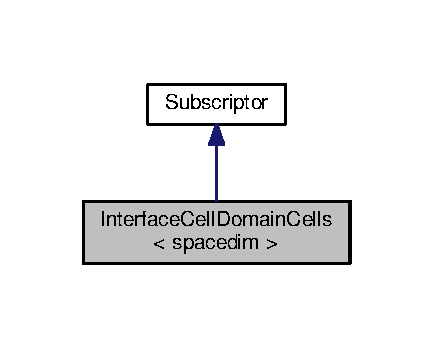
\includegraphics[width=208pt]{class_interface_cell_domain_cells__inherit__graph}
\end{center}
\end{figure}


Collaboration diagram for Interface\+Cell\+Domain\+Cells$<$ spacedim $>$\+:
\nopagebreak
\begin{figure}[H]
\begin{center}
\leavevmode
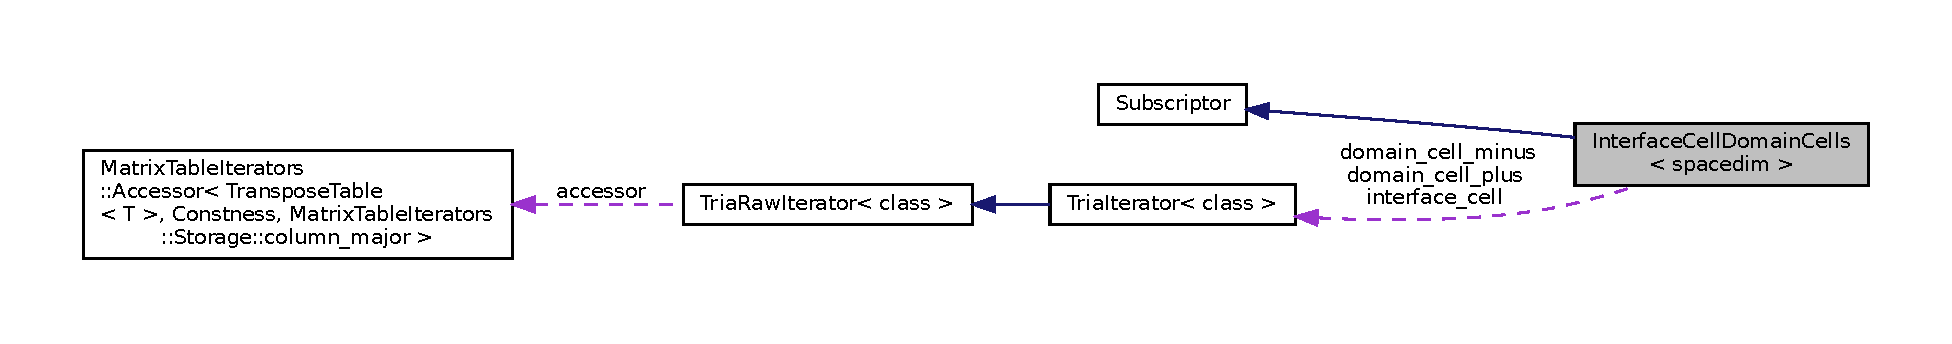
\includegraphics[width=298pt]{class_interface_cell_domain_cells__coll__graph}
\end{center}
\end{figure}
\subsection*{Public Types}
\begin{DoxyCompactItemize}
\item 
typedef {\bf Tria\+Iterator}$<$ {\bf Cell\+Accessor}$<$ spacedim-\/1, spacedim $>$ $>$ \hyperlink{class_interface_cell_domain_cells_ac6c8ada1cde14364575ef0191a278bf8}{Interface\+Cell}
\item 
typedef {\bf Tria\+Iterator}$<$ {\bf Cell\+Accessor}$<$ spacedim, spacedim $>$ $>$ \hyperlink{class_interface_cell_domain_cells_aea8f8f65d0f5021da9c5b8e147b6d587}{Domain\+Cell}
\end{DoxyCompactItemize}
\subsection*{Public Member Functions}
\begin{DoxyCompactItemize}
\item 
\hyperlink{class_interface_cell_domain_cells_a016b875566033b0da13d774081eaeaf4}{Interface\+Cell\+Domain\+Cells} (const \hyperlink{class_interface_cell_domain_cells_aea8f8f65d0f5021da9c5b8e147b6d587}{Domain\+Cell} \&domain\+\_\+cell, const unsigned int face, const \hyperlink{class_interface_cell_domain_cells_ac6c8ada1cde14364575ef0191a278bf8}{Interface\+Cell} \&\hyperlink{class_interface_cell_domain_cells_acabc5a62be3f7742c3c334ae1777fbd5}{interface\+\_\+cell}, const \hyperlink{triangulation__system_8h_a44f3c00e36c1d6e3c389ae693c09b435}{Interface\+Side} interface\+\_\+side)
\item 
\hyperlink{class_interface_cell_domain_cells_a7dae568b2d3c80762d0e1af52c93f279}{$\sim$\+Interface\+Cell\+Domain\+Cells} ()
\item 
std\+::tuple$<$ const {\bf types\+::material\+\_\+id}, const {\bf types\+::material\+\_\+id}, const {\bf types\+::material\+\_\+id} $>$ \hyperlink{class_interface_cell_domain_cells_a9b5388da2f3a61d4340ae4d1b979d6d1}{get\+\_\+material\+\_\+ids} () const 
\end{DoxyCompactItemize}
\subsection*{Public Attributes}
\begin{DoxyCompactItemize}
\item 
const \hyperlink{class_interface_cell_domain_cells_ac6c8ada1cde14364575ef0191a278bf8}{Interface\+Cell} \hyperlink{class_interface_cell_domain_cells_acabc5a62be3f7742c3c334ae1777fbd5}{interface\+\_\+cell}
\item 
const \hyperlink{class_interface_cell_domain_cells_aea8f8f65d0f5021da9c5b8e147b6d587}{Domain\+Cell} \hyperlink{class_interface_cell_domain_cells_ae610a6a7b0ff4a421ee051cb873bbc22}{domain\+\_\+cell\+\_\+minus}
\item 
const unsigned int \hyperlink{class_interface_cell_domain_cells_a51a9eaf54de991f5fa432220b09205cd}{face\+\_\+minus}
\item 
const \hyperlink{class_interface_cell_domain_cells_aea8f8f65d0f5021da9c5b8e147b6d587}{Domain\+Cell} \hyperlink{class_interface_cell_domain_cells_a72c7faaed3a84c546d47960f1064f9df}{domain\+\_\+cell\+\_\+plus}
\item 
const unsigned int \hyperlink{class_interface_cell_domain_cells_a8780275f79c7137ef65df9b7d4039017}{face\+\_\+plus}
\item 
const \hyperlink{triangulation__system_8h_a4cfb8c5e21535951e919b6a6b1023af7}{Interface\+Refinement\+Case} \hyperlink{class_interface_cell_domain_cells_ab1b5469ca5c40256942ea179abbba92c}{refinement\+\_\+case}
\item 
const unsigned int \hyperlink{class_interface_cell_domain_cells_aba7f3e048c6985006988d716cb31aa7d}{subface}
\end{DoxyCompactItemize}
\subsection*{Private Member Functions}
\begin{DoxyCompactItemize}
\item 
\hyperlink{class_interface_cell_domain_cells_a4c0fd73a697833a1257b9341982897de}{Interface\+Cell\+Domain\+Cells} (const std\+::tuple$<$ const \hyperlink{class_interface_cell_domain_cells_ac6c8ada1cde14364575ef0191a278bf8}{Interface\+Cell}, const \hyperlink{class_interface_cell_domain_cells_aea8f8f65d0f5021da9c5b8e147b6d587}{Domain\+Cell}, const unsigned int, const \hyperlink{class_interface_cell_domain_cells_aea8f8f65d0f5021da9c5b8e147b6d587}{Domain\+Cell}, const unsigned int, const \hyperlink{triangulation__system_8h_a4cfb8c5e21535951e919b6a6b1023af7}{Interface\+Refinement\+Case}, const unsigned int $>$ input)
\end{DoxyCompactItemize}
\subsection*{Static Private Member Functions}
\begin{DoxyCompactItemize}
\item 
static std\+::tuple$<$ const \hyperlink{class_interface_cell_domain_cells_ac6c8ada1cde14364575ef0191a278bf8}{Interface\+Cell}, const \hyperlink{class_interface_cell_domain_cells_aea8f8f65d0f5021da9c5b8e147b6d587}{Domain\+Cell}, const unsigned int, const \hyperlink{class_interface_cell_domain_cells_aea8f8f65d0f5021da9c5b8e147b6d587}{Domain\+Cell}, const unsigned int, const \hyperlink{triangulation__system_8h_a4cfb8c5e21535951e919b6a6b1023af7}{Interface\+Refinement\+Case}, const unsigned int $>$ \hyperlink{class_interface_cell_domain_cells_a3f892a73f1f38f7412e549b9e62a8928}{convert\+\_\+constructor\+\_\+inputs} (const \hyperlink{class_interface_cell_domain_cells_aea8f8f65d0f5021da9c5b8e147b6d587}{Domain\+Cell} \&domain\+\_\+cell, const unsigned int face, const \hyperlink{class_interface_cell_domain_cells_ac6c8ada1cde14364575ef0191a278bf8}{Interface\+Cell} \&\hyperlink{class_interface_cell_domain_cells_acabc5a62be3f7742c3c334ae1777fbd5}{interface\+\_\+cell}, const \hyperlink{triangulation__system_8h_a44f3c00e36c1d6e3c389ae693c09b435}{Interface\+Side} interface\+\_\+side)
\end{DoxyCompactItemize}
\subsection*{Additional Inherited Members}


\subsection{Detailed Description}
\subsubsection*{template$<$unsigned int spacedim$>$\\*
class Interface\+Cell\+Domain\+Cells$<$ spacedim $>$}

Objects of this class contain information about an interface cell and the neighboring domain cells.

The \hyperlink{class_interface_cell_domain_cells}{Interface\+Cell\+Domain\+Cells} class inherits from {\bf Subscriptor} in order to be able to check that \hyperlink{class_interface_cell_domain_cells}{Interface\+Cell\+Domain\+Cells} objects are only destroyed when they are not needed anymore by other objects.


\begin{DoxyTemplParams}{Template Parameters}
{\em spacedim} & The spatial dimension into which the interface is embedded. \\
\hline
\end{DoxyTemplParams}


\subsection{Member Typedef Documentation}
\index{Interface\+Cell\+Domain\+Cells@{Interface\+Cell\+Domain\+Cells}!Domain\+Cell@{Domain\+Cell}}
\index{Domain\+Cell@{Domain\+Cell}!Interface\+Cell\+Domain\+Cells@{Interface\+Cell\+Domain\+Cells}}
\subsubsection[{\texorpdfstring{Domain\+Cell}{DomainCell}}]{\setlength{\rightskip}{0pt plus 5cm}template$<$unsigned int spacedim$>$ typedef {\bf Tria\+Iterator}$<${\bf Cell\+Accessor}$<$spacedim, spacedim$>$ $>$ {\bf Interface\+Cell\+Domain\+Cells}$<$ spacedim $>$\+::{\bf Domain\+Cell}}\hypertarget{class_interface_cell_domain_cells_aea8f8f65d0f5021da9c5b8e147b6d587}{}\label{class_interface_cell_domain_cells_aea8f8f65d0f5021da9c5b8e147b6d587}
A convenience typedef for a deal.\+II {\bf Tria\+Iterator} referring to a domain cell \index{Interface\+Cell\+Domain\+Cells@{Interface\+Cell\+Domain\+Cells}!Interface\+Cell@{Interface\+Cell}}
\index{Interface\+Cell@{Interface\+Cell}!Interface\+Cell\+Domain\+Cells@{Interface\+Cell\+Domain\+Cells}}
\subsubsection[{\texorpdfstring{Interface\+Cell}{InterfaceCell}}]{\setlength{\rightskip}{0pt plus 5cm}template$<$unsigned int spacedim$>$ typedef {\bf Tria\+Iterator}$<${\bf Cell\+Accessor}$<$spacedim-\/1, spacedim$>$ $>$ {\bf Interface\+Cell\+Domain\+Cells}$<$ spacedim $>$\+::{\bf Interface\+Cell}}\hypertarget{class_interface_cell_domain_cells_ac6c8ada1cde14364575ef0191a278bf8}{}\label{class_interface_cell_domain_cells_ac6c8ada1cde14364575ef0191a278bf8}
A convenience typedef for a deal.\+II {\bf Tria\+Iterator} referring to an interface cell 

\subsection{Constructor \& Destructor Documentation}
\index{Interface\+Cell\+Domain\+Cells@{Interface\+Cell\+Domain\+Cells}!Interface\+Cell\+Domain\+Cells@{Interface\+Cell\+Domain\+Cells}}
\index{Interface\+Cell\+Domain\+Cells@{Interface\+Cell\+Domain\+Cells}!Interface\+Cell\+Domain\+Cells@{Interface\+Cell\+Domain\+Cells}}
\subsubsection[{\texorpdfstring{Interface\+Cell\+Domain\+Cells(const std\+::tuple$<$ const Interface\+Cell, const Domain\+Cell, const unsigned int, const Domain\+Cell, const unsigned int, const Interface\+Refinement\+Case, const unsigned int $>$ input)}{InterfaceCellDomainCells(const std::tuple< const InterfaceCell, const DomainCell, const unsigned int, const DomainCell, const unsigned int, const InterfaceRefinementCase, const unsigned int > input)}}]{\setlength{\rightskip}{0pt plus 5cm}template$<$unsigned int spacedim$>$ {\bf Interface\+Cell\+Domain\+Cells}$<$ spacedim $>$\+::{\bf Interface\+Cell\+Domain\+Cells} (
\begin{DoxyParamCaption}
\item[{const std\+::tuple$<$ const {\bf Interface\+Cell}, const {\bf Domain\+Cell}, const unsigned int, const {\bf Domain\+Cell}, const unsigned int, const {\bf Interface\+Refinement\+Case}, const unsigned int $>$}]{input}
\end{DoxyParamCaption}
)\hspace{0.3cm}{\ttfamily [private]}}\hypertarget{class_interface_cell_domain_cells_a4c0fd73a697833a1257b9341982897de}{}\label{class_interface_cell_domain_cells_a4c0fd73a697833a1257b9341982897de}
This private constructor is called by the public constructor in order to set up the member variables. The conversion between the input parameters of the public constructor and this private constructor is done by the static member function \hyperlink{class_interface_cell_domain_cells_a3f892a73f1f38f7412e549b9e62a8928}{Interface\+Cell\+Domain\+Cells\+::convert\+\_\+constructor\+\_\+inputs}. Although this indirect approach is a bit awkward, it has the advantage of maintaining constness of the members of this class.


\begin{DoxyParams}[1]{Parameters}
\mbox{\tt in}  & {\em input} & A tuple containing the members \hyperlink{class_interface_cell_domain_cells_acabc5a62be3f7742c3c334ae1777fbd5}{Interface\+Cell\+Domain\+Cells\+::interface\+\_\+cell}, \hyperlink{class_interface_cell_domain_cells_ae610a6a7b0ff4a421ee051cb873bbc22}{Interface\+Cell\+Domain\+Cells\+::domain\+\_\+cell\+\_\+minus}, \hyperlink{class_interface_cell_domain_cells_a51a9eaf54de991f5fa432220b09205cd}{Interface\+Cell\+Domain\+Cells\+::face\+\_\+minus}, \hyperlink{class_interface_cell_domain_cells_a72c7faaed3a84c546d47960f1064f9df}{Interface\+Cell\+Domain\+Cells\+::domain\+\_\+cell\+\_\+plus}, \hyperlink{class_interface_cell_domain_cells_a8780275f79c7137ef65df9b7d4039017}{Interface\+Cell\+Domain\+Cells\+::face\+\_\+plus}, \hyperlink{class_interface_cell_domain_cells_ab1b5469ca5c40256942ea179abbba92c}{Interface\+Cell\+Domain\+Cells\+::refinement\+\_\+case}, \hyperlink{class_interface_cell_domain_cells_aba7f3e048c6985006988d716cb31aa7d}{Interface\+Cell\+Domain\+Cells\+::subface} \\
\hline
\end{DoxyParams}
\index{Interface\+Cell\+Domain\+Cells@{Interface\+Cell\+Domain\+Cells}!Interface\+Cell\+Domain\+Cells@{Interface\+Cell\+Domain\+Cells}}
\index{Interface\+Cell\+Domain\+Cells@{Interface\+Cell\+Domain\+Cells}!Interface\+Cell\+Domain\+Cells@{Interface\+Cell\+Domain\+Cells}}
\subsubsection[{\texorpdfstring{Interface\+Cell\+Domain\+Cells(const Domain\+Cell \&domain\+\_\+cell, const unsigned int face, const Interface\+Cell \&interface\+\_\+cell, const Interface\+Side interface\+\_\+side)}{InterfaceCellDomainCells(const DomainCell &domain_cell, const unsigned int face, const InterfaceCell &interface_cell, const InterfaceSide interface_side)}}]{\setlength{\rightskip}{0pt plus 5cm}template$<$unsigned int spacedim$>$ {\bf Interface\+Cell\+Domain\+Cells}$<$ spacedim $>$\+::{\bf Interface\+Cell\+Domain\+Cells} (
\begin{DoxyParamCaption}
\item[{const {\bf Domain\+Cell} \&}]{domain\+\_\+cell, }
\item[{const unsigned int}]{face, }
\item[{const {\bf Interface\+Cell} \&}]{interface\+\_\+cell, }
\item[{const {\bf Interface\+Side}}]{interface\+\_\+side}
\end{DoxyParamCaption}
)}\hypertarget{class_interface_cell_domain_cells_a016b875566033b0da13d774081eaeaf4}{}\label{class_interface_cell_domain_cells_a016b875566033b0da13d774081eaeaf4}
The public constructor of this class.


\begin{DoxyParams}[1]{Parameters}
\mbox{\tt in}  & {\em domain\+\_\+cell} & An iterator to the domain cell underlying the interface cell {\ttfamily interface\+\_\+cell} \\
\hline
\mbox{\tt in}  & {\em face} & The face number of the domain cell {\ttfamily domain\+\_\+cell} underlying the interface {\ttfamily interface\+\_\+cell} \\
\hline
\mbox{\tt in}  & {\em interface\+\_\+cell} & An iterator to the interface cell, which is defined by the pair {\ttfamily domain\+\_\+cell}, {\ttfamily face}. The constructor will assert on whether the domain cell face defined by the pair {\ttfamily domain\+\_\+cell}, {\ttfamily face} coincides with {\ttfamily interface\+\_\+cell} by checking coincidence of the face / cell centers.\\
\hline
\mbox{\tt in}  & {\em interface\+\_\+side} & The side of the interface cell on which {\ttfamily domain\+\_\+cell} lies \\
\hline
\end{DoxyParams}
\index{Interface\+Cell\+Domain\+Cells@{Interface\+Cell\+Domain\+Cells}!````~Interface\+Cell\+Domain\+Cells@{$\sim$\+Interface\+Cell\+Domain\+Cells}}
\index{````~Interface\+Cell\+Domain\+Cells@{$\sim$\+Interface\+Cell\+Domain\+Cells}!Interface\+Cell\+Domain\+Cells@{Interface\+Cell\+Domain\+Cells}}
\subsubsection[{\texorpdfstring{$\sim$\+Interface\+Cell\+Domain\+Cells()}{~InterfaceCellDomainCells()}}]{\setlength{\rightskip}{0pt plus 5cm}template$<$unsigned int spacedim$>$ {\bf Interface\+Cell\+Domain\+Cells}$<$ spacedim $>$\+::$\sim${\bf Interface\+Cell\+Domain\+Cells} (
\begin{DoxyParamCaption}
{}
\end{DoxyParamCaption}
)}\hypertarget{class_interface_cell_domain_cells_a7dae568b2d3c80762d0e1af52c93f279}{}\label{class_interface_cell_domain_cells_a7dae568b2d3c80762d0e1af52c93f279}
The destructor of \hyperlink{class_interface_cell_domain_cells}{Interface\+Cell\+Domain\+Cells} essentially checks before destruction that the \hyperlink{class_interface_cell_domain_cells}{Interface\+Cell\+Domain\+Cells} object is not used by other objects. If this is the case, the program will be aborted. 

\subsection{Member Function Documentation}
\index{Interface\+Cell\+Domain\+Cells@{Interface\+Cell\+Domain\+Cells}!convert\+\_\+constructor\+\_\+inputs@{convert\+\_\+constructor\+\_\+inputs}}
\index{convert\+\_\+constructor\+\_\+inputs@{convert\+\_\+constructor\+\_\+inputs}!Interface\+Cell\+Domain\+Cells@{Interface\+Cell\+Domain\+Cells}}
\subsubsection[{\texorpdfstring{convert\+\_\+constructor\+\_\+inputs(const Domain\+Cell \&domain\+\_\+cell, const unsigned int face, const Interface\+Cell \&interface\+\_\+cell, const Interface\+Side interface\+\_\+side)}{convert_constructor_inputs(const DomainCell &domain_cell, const unsigned int face, const InterfaceCell &interface_cell, const InterfaceSide interface_side)}}]{\setlength{\rightskip}{0pt plus 5cm}template$<$unsigned int spacedim$>$ static std\+::tuple$<$const {\bf Interface\+Cell}, const {\bf Domain\+Cell}, const unsigned int, const {\bf Domain\+Cell}, const unsigned int, const {\bf Interface\+Refinement\+Case}, const unsigned int$>$ {\bf Interface\+Cell\+Domain\+Cells}$<$ spacedim $>$\+::convert\+\_\+constructor\+\_\+inputs (
\begin{DoxyParamCaption}
\item[{const {\bf Domain\+Cell} \&}]{domain\+\_\+cell, }
\item[{const unsigned int}]{face, }
\item[{const {\bf Interface\+Cell} \&}]{interface\+\_\+cell, }
\item[{const {\bf Interface\+Side}}]{interface\+\_\+side}
\end{DoxyParamCaption}
)\hspace{0.3cm}{\ttfamily [static]}, {\ttfamily [private]}}\hypertarget{class_interface_cell_domain_cells_a3f892a73f1f38f7412e549b9e62a8928}{}\label{class_interface_cell_domain_cells_a3f892a73f1f38f7412e549b9e62a8928}
This method is used internally to convert the inputs of the public constructor into the information required to set up the const members of this class with the private constructor.


\begin{DoxyParams}[1]{Parameters}
\mbox{\tt in}  & {\em domain\+\_\+cell} & An iterator to the domain cell underlying the interface cell {\ttfamily interface\+\_\+cell} \\
\hline
\mbox{\tt in}  & {\em face} & The face number of the domain cell {\ttfamily domain\+\_\+cell} underlying the interface {\ttfamily interface\+\_\+cell} \\
\hline
\mbox{\tt in}  & {\em interface\+\_\+cell} & An iterator to the interface cell, which is defined by the pair {\ttfamily domain\+\_\+cell}, {\ttfamily face}. The constructor will assert on whether the domain cell face defined by the pair {\ttfamily domain\+\_\+cell}, {\ttfamily face} coincides with {\ttfamily interface\+\_\+cell} by checking coincidence of the face / cell centers.\\
\hline
\mbox{\tt in}  & {\em interface\+\_\+side} & The side of interface on which {\ttfamily domain\+\_\+cell} lies\\
\hline
\end{DoxyParams}
\begin{DoxyReturn}{Returns}
A tuple containing the members \hyperlink{class_interface_cell_domain_cells_acabc5a62be3f7742c3c334ae1777fbd5}{Interface\+Cell\+Domain\+Cells\+::interface\+\_\+cell}, \hyperlink{class_interface_cell_domain_cells_ae610a6a7b0ff4a421ee051cb873bbc22}{Interface\+Cell\+Domain\+Cells\+::domain\+\_\+cell\+\_\+minus}, \hyperlink{class_interface_cell_domain_cells_a51a9eaf54de991f5fa432220b09205cd}{Interface\+Cell\+Domain\+Cells\+::face\+\_\+minus}, \hyperlink{class_interface_cell_domain_cells_a72c7faaed3a84c546d47960f1064f9df}{Interface\+Cell\+Domain\+Cells\+::domain\+\_\+cell\+\_\+plus}, \hyperlink{class_interface_cell_domain_cells_a8780275f79c7137ef65df9b7d4039017}{Interface\+Cell\+Domain\+Cells\+::face\+\_\+plus}, \hyperlink{class_interface_cell_domain_cells_ab1b5469ca5c40256942ea179abbba92c}{Interface\+Cell\+Domain\+Cells\+::refinement\+\_\+case}, \hyperlink{class_interface_cell_domain_cells_aba7f3e048c6985006988d716cb31aa7d}{Interface\+Cell\+Domain\+Cells\+::subface} 
\end{DoxyReturn}
\index{Interface\+Cell\+Domain\+Cells@{Interface\+Cell\+Domain\+Cells}!get\+\_\+material\+\_\+ids@{get\+\_\+material\+\_\+ids}}
\index{get\+\_\+material\+\_\+ids@{get\+\_\+material\+\_\+ids}!Interface\+Cell\+Domain\+Cells@{Interface\+Cell\+Domain\+Cells}}
\subsubsection[{\texorpdfstring{get\+\_\+material\+\_\+ids() const }{get_material_ids() const }}]{\setlength{\rightskip}{0pt plus 5cm}template$<$unsigned int spacedim$>$ std\+::tuple$<$const {\bf types\+::material\+\_\+id}, const {\bf types\+::material\+\_\+id}, const {\bf types\+::material\+\_\+id}$>$ {\bf Interface\+Cell\+Domain\+Cells}$<$ spacedim $>$\+::get\+\_\+material\+\_\+ids (
\begin{DoxyParamCaption}
{}
\end{DoxyParamCaption}
) const}\hypertarget{class_interface_cell_domain_cells_a9b5388da2f3a61d4340ae4d1b979d6d1}{}\label{class_interface_cell_domain_cells_a9b5388da2f3a61d4340ae4d1b979d6d1}
\begin{DoxyReturn}{Returns}
This method returns a tuple with the {\bf types\+::material\+\_\+id}s associated with \hyperlink{class_interface_cell_domain_cells_acabc5a62be3f7742c3c334ae1777fbd5}{Interface\+Cell\+Domain\+Cells\+::interface\+\_\+cell}, \hyperlink{class_interface_cell_domain_cells_ae610a6a7b0ff4a421ee051cb873bbc22}{Interface\+Cell\+Domain\+Cells\+::domain\+\_\+cell\+\_\+minus}, \hyperlink{class_interface_cell_domain_cells_a72c7faaed3a84c546d47960f1064f9df}{Interface\+Cell\+Domain\+Cells\+::domain\+\_\+cell\+\_\+plus} (in this order).
\end{DoxyReturn}
If the interface cell is actually at the boundary, the third member of the tuple will be returned as {\bf numbers\+::invalid\+\_\+material\+\_\+id} 

\subsection{Member Data Documentation}
\index{Interface\+Cell\+Domain\+Cells@{Interface\+Cell\+Domain\+Cells}!domain\+\_\+cell\+\_\+minus@{domain\+\_\+cell\+\_\+minus}}
\index{domain\+\_\+cell\+\_\+minus@{domain\+\_\+cell\+\_\+minus}!Interface\+Cell\+Domain\+Cells@{Interface\+Cell\+Domain\+Cells}}
\subsubsection[{\texorpdfstring{domain\+\_\+cell\+\_\+minus}{domain_cell_minus}}]{\setlength{\rightskip}{0pt plus 5cm}template$<$unsigned int spacedim$>$ const {\bf Domain\+Cell} {\bf Interface\+Cell\+Domain\+Cells}$<$ spacedim $>$\+::domain\+\_\+cell\+\_\+minus}\hypertarget{class_interface_cell_domain_cells_ae610a6a7b0ff4a421ee051cb873bbc22}{}\label{class_interface_cell_domain_cells_ae610a6a7b0ff4a421ee051cb873bbc22}
A deal.\+II {\bf Tria\+Iterator} to the domain cell adjacent to the interface cell on the minus side.

\hyperlink{class_interface_cell_domain_cells_ae610a6a7b0ff4a421ee051cb873bbc22}{Interface\+Cell\+Domain\+Cells\+::domain\+\_\+cell\+\_\+minus} is refined to the same degree as \hyperlink{class_interface_cell_domain_cells_acabc5a62be3f7742c3c334ae1777fbd5}{Interface\+Cell\+Domain\+Cells\+::interface\+\_\+cell} if \hyperlink{class_interface_cell_domain_cells_ab1b5469ca5c40256942ea179abbba92c}{Interface\+Cell\+Domain\+Cells\+::refinement\+\_\+case} == {\ttfamily minus\+\_\+is\+\_\+finer} or if \hyperlink{class_interface_cell_domain_cells_ab1b5469ca5c40256942ea179abbba92c}{Interface\+Cell\+Domain\+Cells\+::refinement\+\_\+case} == {\ttfamily equally\+\_\+fine} or if \hyperlink{class_interface_cell_domain_cells_ab1b5469ca5c40256942ea179abbba92c}{Interface\+Cell\+Domain\+Cells\+::refinement\+\_\+case} == {\ttfamily at\+\_\+boundary}. Otherwise, it is once less refined than \hyperlink{class_interface_cell_domain_cells_acabc5a62be3f7742c3c334ae1777fbd5}{Interface\+Cell\+Domain\+Cells\+::interface\+\_\+cell}. \index{Interface\+Cell\+Domain\+Cells@{Interface\+Cell\+Domain\+Cells}!domain\+\_\+cell\+\_\+plus@{domain\+\_\+cell\+\_\+plus}}
\index{domain\+\_\+cell\+\_\+plus@{domain\+\_\+cell\+\_\+plus}!Interface\+Cell\+Domain\+Cells@{Interface\+Cell\+Domain\+Cells}}
\subsubsection[{\texorpdfstring{domain\+\_\+cell\+\_\+plus}{domain_cell_plus}}]{\setlength{\rightskip}{0pt plus 5cm}template$<$unsigned int spacedim$>$ const {\bf Domain\+Cell} {\bf Interface\+Cell\+Domain\+Cells}$<$ spacedim $>$\+::domain\+\_\+cell\+\_\+plus}\hypertarget{class_interface_cell_domain_cells_a72c7faaed3a84c546d47960f1064f9df}{}\label{class_interface_cell_domain_cells_a72c7faaed3a84c546d47960f1064f9df}
A deal.\+II {\bf Tria\+Iterator} to the domain cell adjacent to the interface cell on the plus side.

\hyperlink{class_interface_cell_domain_cells_a72c7faaed3a84c546d47960f1064f9df}{Interface\+Cell\+Domain\+Cells\+::domain\+\_\+cell\+\_\+plus} is refined to the same degree as \hyperlink{class_interface_cell_domain_cells_acabc5a62be3f7742c3c334ae1777fbd5}{Interface\+Cell\+Domain\+Cells\+::interface\+\_\+cell} if \hyperlink{class_interface_cell_domain_cells_ab1b5469ca5c40256942ea179abbba92c}{Interface\+Cell\+Domain\+Cells\+::refinement\+\_\+case} == {\ttfamily plus\+\_\+is\+\_\+finer} or if \hyperlink{class_interface_cell_domain_cells_ab1b5469ca5c40256942ea179abbba92c}{Interface\+Cell\+Domain\+Cells\+::refinement\+\_\+case} == {\ttfamily equally\+\_\+fine}; and it is once less refined than \hyperlink{class_interface_cell_domain_cells_acabc5a62be3f7742c3c334ae1777fbd5}{Interface\+Cell\+Domain\+Cells\+::interface\+\_\+cell} if \hyperlink{class_interface_cell_domain_cells_ab1b5469ca5c40256942ea179abbba92c}{Interface\+Cell\+Domain\+Cells\+::refinement\+\_\+case} == {\ttfamily minus\+\_\+is\+\_\+finer}. Otherwise, the interface is actually a boundary, in which case \hyperlink{class_interface_cell_domain_cells_a72c7faaed3a84c546d47960f1064f9df}{Interface\+Cell\+Domain\+Cells\+::domain\+\_\+cell\+\_\+plus} is set to the same cell as \hyperlink{class_interface_cell_domain_cells_ae610a6a7b0ff4a421ee051cb873bbc22}{Interface\+Cell\+Domain\+Cells\+::domain\+\_\+cell\+\_\+minus}. \index{Interface\+Cell\+Domain\+Cells@{Interface\+Cell\+Domain\+Cells}!face\+\_\+minus@{face\+\_\+minus}}
\index{face\+\_\+minus@{face\+\_\+minus}!Interface\+Cell\+Domain\+Cells@{Interface\+Cell\+Domain\+Cells}}
\subsubsection[{\texorpdfstring{face\+\_\+minus}{face_minus}}]{\setlength{\rightskip}{0pt plus 5cm}template$<$unsigned int spacedim$>$ const unsigned int {\bf Interface\+Cell\+Domain\+Cells}$<$ spacedim $>$\+::face\+\_\+minus}\hypertarget{class_interface_cell_domain_cells_a51a9eaf54de991f5fa432220b09205cd}{}\label{class_interface_cell_domain_cells_a51a9eaf54de991f5fa432220b09205cd}
The face number of the face of the domain cell on the minus side lying on the interface \index{Interface\+Cell\+Domain\+Cells@{Interface\+Cell\+Domain\+Cells}!face\+\_\+plus@{face\+\_\+plus}}
\index{face\+\_\+plus@{face\+\_\+plus}!Interface\+Cell\+Domain\+Cells@{Interface\+Cell\+Domain\+Cells}}
\subsubsection[{\texorpdfstring{face\+\_\+plus}{face_plus}}]{\setlength{\rightskip}{0pt plus 5cm}template$<$unsigned int spacedim$>$ const unsigned int {\bf Interface\+Cell\+Domain\+Cells}$<$ spacedim $>$\+::face\+\_\+plus}\hypertarget{class_interface_cell_domain_cells_a8780275f79c7137ef65df9b7d4039017}{}\label{class_interface_cell_domain_cells_a8780275f79c7137ef65df9b7d4039017}
The face number of the face of the domain cell on the plus side lying on the interface \index{Interface\+Cell\+Domain\+Cells@{Interface\+Cell\+Domain\+Cells}!interface\+\_\+cell@{interface\+\_\+cell}}
\index{interface\+\_\+cell@{interface\+\_\+cell}!Interface\+Cell\+Domain\+Cells@{Interface\+Cell\+Domain\+Cells}}
\subsubsection[{\texorpdfstring{interface\+\_\+cell}{interface_cell}}]{\setlength{\rightskip}{0pt plus 5cm}template$<$unsigned int spacedim$>$ const {\bf Interface\+Cell} {\bf Interface\+Cell\+Domain\+Cells}$<$ spacedim $>$\+::interface\+\_\+cell}\hypertarget{class_interface_cell_domain_cells_acabc5a62be3f7742c3c334ae1777fbd5}{}\label{class_interface_cell_domain_cells_acabc5a62be3f7742c3c334ae1777fbd5}
A deal.\+II {\bf Tria\+Iterator} to the interface cell \index{Interface\+Cell\+Domain\+Cells@{Interface\+Cell\+Domain\+Cells}!refinement\+\_\+case@{refinement\+\_\+case}}
\index{refinement\+\_\+case@{refinement\+\_\+case}!Interface\+Cell\+Domain\+Cells@{Interface\+Cell\+Domain\+Cells}}
\subsubsection[{\texorpdfstring{refinement\+\_\+case}{refinement_case}}]{\setlength{\rightskip}{0pt plus 5cm}template$<$unsigned int spacedim$>$ const {\bf Interface\+Refinement\+Case} {\bf Interface\+Cell\+Domain\+Cells}$<$ spacedim $>$\+::refinement\+\_\+case}\hypertarget{class_interface_cell_domain_cells_ab1b5469ca5c40256942ea179abbba92c}{}\label{class_interface_cell_domain_cells_ab1b5469ca5c40256942ea179abbba92c}
The refinement situation at the interface cell. See \hyperlink{triangulation__system_8h_a4cfb8c5e21535951e919b6a6b1023af7}{Interface\+Refinement\+Case} for further documentation. \index{Interface\+Cell\+Domain\+Cells@{Interface\+Cell\+Domain\+Cells}!subface@{subface}}
\index{subface@{subface}!Interface\+Cell\+Domain\+Cells@{Interface\+Cell\+Domain\+Cells}}
\subsubsection[{\texorpdfstring{subface}{subface}}]{\setlength{\rightskip}{0pt plus 5cm}template$<$unsigned int spacedim$>$ const unsigned int {\bf Interface\+Cell\+Domain\+Cells}$<$ spacedim $>$\+::subface}\hypertarget{class_interface_cell_domain_cells_aba7f3e048c6985006988d716cb31aa7d}{}\label{class_interface_cell_domain_cells_aba7f3e048c6985006988d716cb31aa7d}
This member applies only to the case, where the domain mesh on one side of the interface cell is refined differently than the domain mesh on the other side (i.\+e., where \hyperlink{class_interface_cell_domain_cells_ab1b5469ca5c40256942ea179abbba92c}{Interface\+Cell\+Domain\+Cells\+::refinement\+\_\+case} == {\ttfamily minus\+\_\+is\+\_\+finer} or \hyperlink{class_interface_cell_domain_cells_ab1b5469ca5c40256942ea179abbba92c}{Interface\+Cell\+Domain\+Cells\+::refinement\+\_\+case} == {\ttfamily plus\+\_\+is\+\_\+finer}). It represents the subface of the domain cell face on the coarser side of the interface coinciding with the interface cell (and, by assumption on the properties of the meshes, with the domain cell face on the finer side of the interface as well).

See also the documentation of the {\bf Cell\+Accessor$<$dim, spacedim$>$\+::neighbor\+\_\+of\+\_\+coarser\+\_\+neighbor()} method. 

The documentation for this class was generated from the following file\+:\begin{DoxyCompactItemize}
\item 
/home/sst/code/\+Galerkin\+Tools/\+Galerkin\+Tools/include/galerkin\+\_\+tools/\hyperlink{triangulation__system_8h}{triangulation\+\_\+system.\+h}\end{DoxyCompactItemize}

\hypertarget{class_interface_cell_domain_cells_do_f}{}\doxysection{Interface\+Cell\+Domain\+Cells\+DoF$<$ spacedim $>$ Class Template Reference}
\label{class_interface_cell_domain_cells_do_f}\index{InterfaceCellDomainCellsDoF$<$ spacedim $>$@{InterfaceCellDomainCellsDoF$<$ spacedim $>$}}


{\ttfamily \#include $<$dof\+\_\+handler\+\_\+system.\+h$>$}



Inheritance diagram for Interface\+Cell\+Domain\+Cells\+DoF$<$ spacedim $>$\+:\nopagebreak
\begin{figure}[H]
\begin{center}
\leavevmode
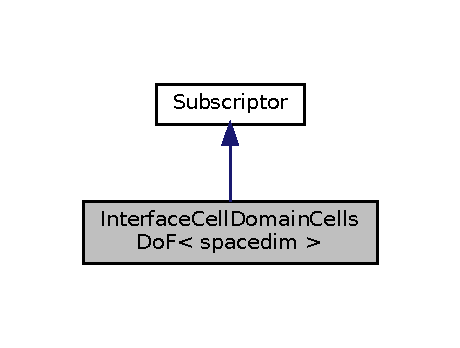
\includegraphics[width=221pt]{class_interface_cell_domain_cells_do_f__inherit__graph}
\end{center}
\end{figure}


Collaboration diagram for Interface\+Cell\+Domain\+Cells\+DoF$<$ spacedim $>$\+:\nopagebreak
\begin{figure}[H]
\begin{center}
\leavevmode
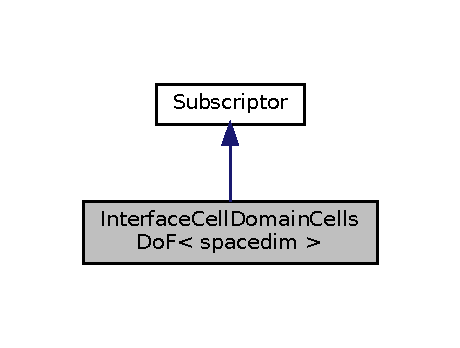
\includegraphics[width=221pt]{class_interface_cell_domain_cells_do_f__coll__graph}
\end{center}
\end{figure}
\doxysubsection*{Public Types}
\begin{DoxyCompactItemize}
\item 
typedef \textbf{ Tria\+Iterator}$<$ \textbf{ Cell\+Accessor}$<$ spacedim-\/1, spacedim $>$ $>$ \mbox{\hyperlink{class_interface_cell_domain_cells_do_f_a55783857b93a31baac5a6e6ee3dad22f}{Interface\+Cell}}
\item 
typedef \textbf{ Do\+F\+Handler}$<$ spacedim-\/1, spacedim $>$\+::\textbf{ cell\+\_\+iterator} \mbox{\hyperlink{class_interface_cell_domain_cells_do_f_ac24e469237fddaf0310a5f818ba13afd}{Interface\+Cell\+DoF}}
\item 
typedef \textbf{ Tria\+Iterator}$<$ \textbf{ Cell\+Accessor}$<$ spacedim, spacedim $>$ $>$ \mbox{\hyperlink{class_interface_cell_domain_cells_do_f_a0d0b12a444adb340e1ffc2dd23d77902}{Domain\+Cell}}
\item 
typedef \textbf{ Do\+F\+Handler}$<$ spacedim, spacedim $>$\+::\textbf{ cell\+\_\+iterator} \mbox{\hyperlink{class_interface_cell_domain_cells_do_f_a78225607ebf9880311f4fdeb30c5a89d}{Domain\+Cell\+DoF}}
\end{DoxyCompactItemize}
\doxysubsection*{Public Member Functions}
\begin{DoxyCompactItemize}
\item 
\mbox{\hyperlink{class_interface_cell_domain_cells_do_f_a79a88327d88717a2c3381fe7131b435d}{Interface\+Cell\+Domain\+Cells\+DoF}} (const \mbox{\hyperlink{class_interface_cell_domain_cells}{Interface\+Cell\+Domain\+Cells}}$<$ spacedim $>$ \&interface\+\_\+cell\+\_\+domain\+\_\+cells, const \mbox{\hyperlink{class_do_f_handler_system}{Do\+F\+Handler\+System}}$<$ spacedim $>$ \&dof\+\_\+handler\+\_\+system)
\item 
\mbox{\hyperlink{class_interface_cell_domain_cells_do_f_a090e1536777928b78dff7fa7b1021a1e}{$\sim$\+Interface\+Cell\+Domain\+Cells\+DoF}} ()
\item 
std\+::tuple$<$ const \textbf{ types\+::material\+\_\+id}, const \textbf{ types\+::material\+\_\+id}, const \textbf{ types\+::material\+\_\+id} $>$ \mbox{\hyperlink{class_interface_cell_domain_cells_do_f_a4823f0f9c791b61d6fb75699952464e5}{get\+\_\+material\+\_\+ids}} () const
\item 
void \mbox{\hyperlink{class_interface_cell_domain_cells_do_f_ab6ff11f2adfa7cd1fd13a2d3e9b3b130}{get\+\_\+dof\+\_\+indices\+\_\+local\+\_\+global\+\_\+interface}} (\textbf{ std\+::vector}$<$ unsigned int $>$ \&dof\+\_\+indices\+\_\+local\+\_\+global, \textbf{ std\+::vector}$<$ unsigned int $>$ \&dof\+\_\+indices\+\_\+local\+\_\+global\+\_\+minus, \textbf{ std\+::vector}$<$ unsigned int $>$ \&dof\+\_\+indices\+\_\+local\+\_\+global\+\_\+plus) const
\item 
void \mbox{\hyperlink{class_interface_cell_domain_cells_do_f_a69d8ac580b83b2469ba1cc611bb5776b}{get\+\_\+dof\+\_\+indices\+\_\+local\+\_\+global\+\_\+interface}} (\textbf{ std\+::vector}$<$ unsigned int $>$ \&dof\+\_\+indices\+\_\+local\+\_\+global) const
\end{DoxyCompactItemize}
\doxysubsection*{Public Attributes}
\begin{DoxyCompactItemize}
\item 
const \mbox{\hyperlink{class_interface_cell_do_f_iterator}{Interface\+Cell\+Do\+F\+Iterator}}$<$ spacedim $>$ \mbox{\hyperlink{class_interface_cell_domain_cells_do_f_a5fe7922af91545598d89c77ba42a59da}{interface\+\_\+cell}}
\item 
const \mbox{\hyperlink{class_domain_cell_do_f_iterator}{Domain\+Cell\+Do\+F\+Iterator}}$<$ spacedim $>$ \mbox{\hyperlink{class_interface_cell_domain_cells_do_f_ac8c84df4298d2d5be54dc8bf81e48c4b}{domain\+\_\+cell\+\_\+minus}}
\item 
const unsigned int \mbox{\hyperlink{class_interface_cell_domain_cells_do_f_a01fc12497d44b06c7a325ea8f0b2ad28}{face\+\_\+minus}}
\item 
const \mbox{\hyperlink{class_domain_cell_do_f_iterator}{Domain\+Cell\+Do\+F\+Iterator}}$<$ spacedim $>$ \mbox{\hyperlink{class_interface_cell_domain_cells_do_f_a8fd9dbd3a1e53023ecca7917b004bab1}{domain\+\_\+cell\+\_\+plus}}
\item 
const unsigned int \mbox{\hyperlink{class_interface_cell_domain_cells_do_f_afcb7abea75dfc6e310493a6ff9aadcf6}{face\+\_\+plus}}
\item 
const \mbox{\hyperlink{triangulation__system_8h_a4cfb8c5e21535951e919b6a6b1023af7}{Interface\+Refinement\+Case}} \mbox{\hyperlink{class_interface_cell_domain_cells_do_f_aebb7e5f13d079fc83f98f67bcfcc6de3}{refinement\+\_\+case}}
\item 
const unsigned int \mbox{\hyperlink{class_interface_cell_domain_cells_do_f_ac0f33cbe60afdc4f5856ea39a085ed1a}{subface}}
\end{DoxyCompactItemize}
\doxysubsection*{Additional Inherited Members}


\doxysubsection{Detailed Description}
\subsubsection*{template$<$unsigned int spacedim$>$\newline
class Interface\+Cell\+Domain\+Cells\+Do\+F$<$ spacedim $>$}

This class is the equivalent to \mbox{\hyperlink{class_interface_cell_domain_cells}{Interface\+Cell\+Domain\+Cells}} with information about the degrees of freedom associated with the interface cell and the neighboring domain cells

The \mbox{\hyperlink{class_interface_cell_domain_cells_do_f}{Interface\+Cell\+Domain\+Cells\+DoF}} class inherits from \textbf{ Subscriptor} in order to be able to check that \mbox{\hyperlink{class_interface_cell_domain_cells_do_f}{Interface\+Cell\+Domain\+Cells\+DoF}} objects are only destroyed when they are not needed anymore by other objects.


\begin{DoxyTemplParams}{Template Parameters}
{\em spacedim} & The spatial dimension into which the interface is embedded. \\
\hline
\end{DoxyTemplParams}


\doxysubsection{Member Typedef Documentation}
\mbox{\Hypertarget{class_interface_cell_domain_cells_do_f_a0d0b12a444adb340e1ffc2dd23d77902}\label{class_interface_cell_domain_cells_do_f_a0d0b12a444adb340e1ffc2dd23d77902}} 
\index{InterfaceCellDomainCellsDoF$<$ spacedim $>$@{InterfaceCellDomainCellsDoF$<$ spacedim $>$}!DomainCell@{DomainCell}}
\index{DomainCell@{DomainCell}!InterfaceCellDomainCellsDoF$<$ spacedim $>$@{InterfaceCellDomainCellsDoF$<$ spacedim $>$}}
\doxysubsubsection{\texorpdfstring{DomainCell}{DomainCell}}
{\footnotesize\ttfamily template$<$unsigned int spacedim$>$ \\
typedef \textbf{ Tria\+Iterator}$<$\textbf{ Cell\+Accessor}$<$spacedim, spacedim$>$ $>$ \mbox{\hyperlink{class_interface_cell_domain_cells_do_f}{Interface\+Cell\+Domain\+Cells\+DoF}}$<$ spacedim $>$\+::\mbox{\hyperlink{class_interface_cell_domain_cells_do_f_a0d0b12a444adb340e1ffc2dd23d77902}{Domain\+Cell}}}

A convenience typedef for a deal.\+II \textbf{ Tria\+Iterator} referring to a domain cell \mbox{\Hypertarget{class_interface_cell_domain_cells_do_f_a78225607ebf9880311f4fdeb30c5a89d}\label{class_interface_cell_domain_cells_do_f_a78225607ebf9880311f4fdeb30c5a89d}} 
\index{InterfaceCellDomainCellsDoF$<$ spacedim $>$@{InterfaceCellDomainCellsDoF$<$ spacedim $>$}!DomainCellDoF@{DomainCellDoF}}
\index{DomainCellDoF@{DomainCellDoF}!InterfaceCellDomainCellsDoF$<$ spacedim $>$@{InterfaceCellDomainCellsDoF$<$ spacedim $>$}}
\doxysubsubsection{\texorpdfstring{DomainCellDoF}{DomainCellDoF}}
{\footnotesize\ttfamily template$<$unsigned int spacedim$>$ \\
typedef \textbf{ Do\+F\+Handler}$<$spacedim, spacedim$>$\+::\textbf{ cell\+\_\+iterator} \mbox{\hyperlink{class_interface_cell_domain_cells_do_f}{Interface\+Cell\+Domain\+Cells\+DoF}}$<$ spacedim $>$\+::\mbox{\hyperlink{class_interface_cell_domain_cells_do_f_a78225607ebf9880311f4fdeb30c5a89d}{Domain\+Cell\+DoF}}}

A convenience typedef for a deal.\+II cell iterator referring to a domain cell (with dof information) \mbox{\Hypertarget{class_interface_cell_domain_cells_do_f_a55783857b93a31baac5a6e6ee3dad22f}\label{class_interface_cell_domain_cells_do_f_a55783857b93a31baac5a6e6ee3dad22f}} 
\index{InterfaceCellDomainCellsDoF$<$ spacedim $>$@{InterfaceCellDomainCellsDoF$<$ spacedim $>$}!InterfaceCell@{InterfaceCell}}
\index{InterfaceCell@{InterfaceCell}!InterfaceCellDomainCellsDoF$<$ spacedim $>$@{InterfaceCellDomainCellsDoF$<$ spacedim $>$}}
\doxysubsubsection{\texorpdfstring{InterfaceCell}{InterfaceCell}}
{\footnotesize\ttfamily template$<$unsigned int spacedim$>$ \\
typedef \textbf{ Tria\+Iterator}$<$\textbf{ Cell\+Accessor}$<$spacedim-\/1, spacedim$>$ $>$ \mbox{\hyperlink{class_interface_cell_domain_cells_do_f}{Interface\+Cell\+Domain\+Cells\+DoF}}$<$ spacedim $>$\+::\mbox{\hyperlink{class_interface_cell_domain_cells_do_f_a55783857b93a31baac5a6e6ee3dad22f}{Interface\+Cell}}}

A convenience typedef for a deal.\+II \textbf{ Tria\+Iterator} referring to an interface cell \mbox{\Hypertarget{class_interface_cell_domain_cells_do_f_ac24e469237fddaf0310a5f818ba13afd}\label{class_interface_cell_domain_cells_do_f_ac24e469237fddaf0310a5f818ba13afd}} 
\index{InterfaceCellDomainCellsDoF$<$ spacedim $>$@{InterfaceCellDomainCellsDoF$<$ spacedim $>$}!InterfaceCellDoF@{InterfaceCellDoF}}
\index{InterfaceCellDoF@{InterfaceCellDoF}!InterfaceCellDomainCellsDoF$<$ spacedim $>$@{InterfaceCellDomainCellsDoF$<$ spacedim $>$}}
\doxysubsubsection{\texorpdfstring{InterfaceCellDoF}{InterfaceCellDoF}}
{\footnotesize\ttfamily template$<$unsigned int spacedim$>$ \\
typedef \textbf{ Do\+F\+Handler}$<$spacedim-\/1, spacedim$>$\+::\textbf{ cell\+\_\+iterator} \mbox{\hyperlink{class_interface_cell_domain_cells_do_f}{Interface\+Cell\+Domain\+Cells\+DoF}}$<$ spacedim $>$\+::\mbox{\hyperlink{class_interface_cell_domain_cells_do_f_ac24e469237fddaf0310a5f818ba13afd}{Interface\+Cell\+DoF}}}

A convenience typedef for a deal.\+II cell iterator referring to an interface cell (with dof information) 

\doxysubsection{Constructor \& Destructor Documentation}
\mbox{\Hypertarget{class_interface_cell_domain_cells_do_f_a79a88327d88717a2c3381fe7131b435d}\label{class_interface_cell_domain_cells_do_f_a79a88327d88717a2c3381fe7131b435d}} 
\index{InterfaceCellDomainCellsDoF$<$ spacedim $>$@{InterfaceCellDomainCellsDoF$<$ spacedim $>$}!InterfaceCellDomainCellsDoF@{InterfaceCellDomainCellsDoF}}
\index{InterfaceCellDomainCellsDoF@{InterfaceCellDomainCellsDoF}!InterfaceCellDomainCellsDoF$<$ spacedim $>$@{InterfaceCellDomainCellsDoF$<$ spacedim $>$}}
\doxysubsubsection{\texorpdfstring{InterfaceCellDomainCellsDoF()}{InterfaceCellDomainCellsDoF()}}
{\footnotesize\ttfamily template$<$unsigned int spacedim$>$ \\
\mbox{\hyperlink{class_interface_cell_domain_cells_do_f}{Interface\+Cell\+Domain\+Cells\+DoF}}$<$ spacedim $>$\+::\mbox{\hyperlink{class_interface_cell_domain_cells_do_f}{Interface\+Cell\+Domain\+Cells\+DoF}} (\begin{DoxyParamCaption}\item[{const \mbox{\hyperlink{class_interface_cell_domain_cells}{Interface\+Cell\+Domain\+Cells}}$<$ spacedim $>$ \&}]{interface\+\_\+cell\+\_\+domain\+\_\+cells,  }\item[{const \mbox{\hyperlink{class_do_f_handler_system}{Do\+F\+Handler\+System}}$<$ spacedim $>$ \&}]{dof\+\_\+handler\+\_\+system }\end{DoxyParamCaption})}

This constructor constructs an \mbox{\hyperlink{class_interface_cell_domain_cells_do_f}{Interface\+Cell\+Domain\+Cells\+DoF}} object from a corresponding \mbox{\hyperlink{class_interface_cell_domain_cells}{Interface\+Cell\+Domain\+Cells}} object and the \mbox{\hyperlink{class_do_f_handler_system}{Do\+F\+Handler\+System}}.


\begin{DoxyParams}[1]{Parameters}
\mbox{\texttt{ in}}  & {\em interface\+\_\+cell\+\_\+domain\+\_\+cells} & \mbox{\hyperlink{class_interface_cell_domain_cells}{Interface\+Cell\+Domain\+Cells}} object \\
\hline
\mbox{\texttt{ in}}  & {\em dof\+\_\+handler\+\_\+system} & the \mbox{\hyperlink{class_do_f_handler_system}{Do\+F\+Handler\+System}} \\
\hline
\end{DoxyParams}
\mbox{\Hypertarget{class_interface_cell_domain_cells_do_f_a090e1536777928b78dff7fa7b1021a1e}\label{class_interface_cell_domain_cells_do_f_a090e1536777928b78dff7fa7b1021a1e}} 
\index{InterfaceCellDomainCellsDoF$<$ spacedim $>$@{InterfaceCellDomainCellsDoF$<$ spacedim $>$}!````~InterfaceCellDomainCellsDoF@{$\sim$InterfaceCellDomainCellsDoF}}
\index{````~InterfaceCellDomainCellsDoF@{$\sim$InterfaceCellDomainCellsDoF}!InterfaceCellDomainCellsDoF$<$ spacedim $>$@{InterfaceCellDomainCellsDoF$<$ spacedim $>$}}
\doxysubsubsection{\texorpdfstring{$\sim$InterfaceCellDomainCellsDoF()}{~InterfaceCellDomainCellsDoF()}}
{\footnotesize\ttfamily template$<$unsigned int spacedim$>$ \\
\mbox{\hyperlink{class_interface_cell_domain_cells_do_f}{Interface\+Cell\+Domain\+Cells\+DoF}}$<$ spacedim $>$\+::$\sim$\mbox{\hyperlink{class_interface_cell_domain_cells_do_f}{Interface\+Cell\+Domain\+Cells\+DoF}} (\begin{DoxyParamCaption}{ }\end{DoxyParamCaption})}

The destructor of \mbox{\hyperlink{class_interface_cell_domain_cells_do_f}{Interface\+Cell\+Domain\+Cells\+DoF}} essentially checks before destruction that the \mbox{\hyperlink{class_interface_cell_domain_cells_do_f}{Interface\+Cell\+Domain\+Cells\+DoF}} object is not used by other objects. If this is the case, the program will be aborted. 

\doxysubsection{Member Function Documentation}
\mbox{\Hypertarget{class_interface_cell_domain_cells_do_f_a69d8ac580b83b2469ba1cc611bb5776b}\label{class_interface_cell_domain_cells_do_f_a69d8ac580b83b2469ba1cc611bb5776b}} 
\index{InterfaceCellDomainCellsDoF$<$ spacedim $>$@{InterfaceCellDomainCellsDoF$<$ spacedim $>$}!get\_dof\_indices\_local\_global\_interface@{get\_dof\_indices\_local\_global\_interface}}
\index{get\_dof\_indices\_local\_global\_interface@{get\_dof\_indices\_local\_global\_interface}!InterfaceCellDomainCellsDoF$<$ spacedim $>$@{InterfaceCellDomainCellsDoF$<$ spacedim $>$}}
\doxysubsubsection{\texorpdfstring{get\_dof\_indices\_local\_global\_interface()}{get\_dof\_indices\_local\_global\_interface()}\hspace{0.1cm}{\footnotesize\ttfamily [1/2]}}
{\footnotesize\ttfamily template$<$unsigned int spacedim$>$ \\
void \mbox{\hyperlink{class_interface_cell_domain_cells_do_f}{Interface\+Cell\+Domain\+Cells\+DoF}}$<$ spacedim $>$\+::get\+\_\+dof\+\_\+indices\+\_\+local\+\_\+global\+\_\+interface (\begin{DoxyParamCaption}\item[{\textbf{ std\+::vector}$<$ unsigned int $>$ \&}]{dof\+\_\+indices\+\_\+local\+\_\+global }\end{DoxyParamCaption}) const}

Method to get the map between local and global dof indices related to the interface cell \mbox{\hyperlink{class_interface_cell_domain_cells_do_f_a5fe7922af91545598d89c77ba42a59da}{Interface\+Cell\+Domain\+Cells\+Do\+F\+::interface\+\_\+cell}}.


\begin{DoxyParams}[1]{Parameters}
\mbox{\texttt{ out}}  & {\em dof\+\_\+indices\+\_\+local\+\_\+global} & mapping between local dof indices and global ones on \mbox{\hyperlink{class_interface_cell_domain_cells_do_f_a5fe7922af91545598d89c77ba42a59da}{Interface\+Cell\+Domain\+Cells\+Do\+F\+::interface\+\_\+cell}} \\
\hline
\end{DoxyParams}
\mbox{\Hypertarget{class_interface_cell_domain_cells_do_f_ab6ff11f2adfa7cd1fd13a2d3e9b3b130}\label{class_interface_cell_domain_cells_do_f_ab6ff11f2adfa7cd1fd13a2d3e9b3b130}} 
\index{InterfaceCellDomainCellsDoF$<$ spacedim $>$@{InterfaceCellDomainCellsDoF$<$ spacedim $>$}!get\_dof\_indices\_local\_global\_interface@{get\_dof\_indices\_local\_global\_interface}}
\index{get\_dof\_indices\_local\_global\_interface@{get\_dof\_indices\_local\_global\_interface}!InterfaceCellDomainCellsDoF$<$ spacedim $>$@{InterfaceCellDomainCellsDoF$<$ spacedim $>$}}
\doxysubsubsection{\texorpdfstring{get\_dof\_indices\_local\_global\_interface()}{get\_dof\_indices\_local\_global\_interface()}\hspace{0.1cm}{\footnotesize\ttfamily [2/2]}}
{\footnotesize\ttfamily template$<$unsigned int spacedim$>$ \\
void \mbox{\hyperlink{class_interface_cell_domain_cells_do_f}{Interface\+Cell\+Domain\+Cells\+DoF}}$<$ spacedim $>$\+::get\+\_\+dof\+\_\+indices\+\_\+local\+\_\+global\+\_\+interface (\begin{DoxyParamCaption}\item[{\textbf{ std\+::vector}$<$ unsigned int $>$ \&}]{dof\+\_\+indices\+\_\+local\+\_\+global,  }\item[{\textbf{ std\+::vector}$<$ unsigned int $>$ \&}]{dof\+\_\+indices\+\_\+local\+\_\+global\+\_\+minus,  }\item[{\textbf{ std\+::vector}$<$ unsigned int $>$ \&}]{dof\+\_\+indices\+\_\+local\+\_\+global\+\_\+plus }\end{DoxyParamCaption}) const}

Method to get the maps between local and global dof indices related to the interface cell \mbox{\hyperlink{class_interface_cell_domain_cells_do_f_a5fe7922af91545598d89c77ba42a59da}{Interface\+Cell\+Domain\+Cells\+Do\+F\+::interface\+\_\+cell}} and the neighboring domain cells \mbox{\hyperlink{class_interface_cell_domain_cells_do_f_ac8c84df4298d2d5be54dc8bf81e48c4b}{Interface\+Cell\+Domain\+Cells\+Do\+F\+::domain\+\_\+cell\+\_\+minus}} and \mbox{\hyperlink{class_interface_cell_domain_cells_do_f_a8fd9dbd3a1e53023ecca7917b004bab1}{Interface\+Cell\+Domain\+Cells\+Do\+F\+::domain\+\_\+cell\+\_\+plus}}.


\begin{DoxyParams}[1]{Parameters}
\mbox{\texttt{ out}}  & {\em dof\+\_\+indices\+\_\+local\+\_\+global} & mapping between local dof indices and global ones on \mbox{\hyperlink{class_interface_cell_domain_cells_do_f_a5fe7922af91545598d89c77ba42a59da}{Interface\+Cell\+Domain\+Cells\+Do\+F\+::interface\+\_\+cell}}\\
\hline
\mbox{\texttt{ out}}  & {\em dof\+\_\+indices\+\_\+local\+\_\+global\+\_\+minus} & mapping between local dof indices and global ones on \mbox{\hyperlink{class_interface_cell_domain_cells_do_f_ac8c84df4298d2d5be54dc8bf81e48c4b}{Interface\+Cell\+Domain\+Cells\+Do\+F\+::domain\+\_\+cell\+\_\+minus}}\\
\hline
\mbox{\texttt{ out}}  & {\em dof\+\_\+indices\+\_\+local\+\_\+global\+\_\+plus} & mapping between local dof indices and global ones on \mbox{\hyperlink{class_interface_cell_domain_cells_do_f_a8fd9dbd3a1e53023ecca7917b004bab1}{Interface\+Cell\+Domain\+Cells\+Do\+F\+::domain\+\_\+cell\+\_\+plus}} \\
\hline
\end{DoxyParams}
\mbox{\Hypertarget{class_interface_cell_domain_cells_do_f_a4823f0f9c791b61d6fb75699952464e5}\label{class_interface_cell_domain_cells_do_f_a4823f0f9c791b61d6fb75699952464e5}} 
\index{InterfaceCellDomainCellsDoF$<$ spacedim $>$@{InterfaceCellDomainCellsDoF$<$ spacedim $>$}!get\_material\_ids@{get\_material\_ids}}
\index{get\_material\_ids@{get\_material\_ids}!InterfaceCellDomainCellsDoF$<$ spacedim $>$@{InterfaceCellDomainCellsDoF$<$ spacedim $>$}}
\doxysubsubsection{\texorpdfstring{get\_material\_ids()}{get\_material\_ids()}}
{\footnotesize\ttfamily template$<$unsigned int spacedim$>$ \\
std\+::tuple$<$const \textbf{ types\+::material\+\_\+id}, const \textbf{ types\+::material\+\_\+id}, const \textbf{ types\+::material\+\_\+id}$>$ \mbox{\hyperlink{class_interface_cell_domain_cells_do_f}{Interface\+Cell\+Domain\+Cells\+DoF}}$<$ spacedim $>$\+::get\+\_\+material\+\_\+ids (\begin{DoxyParamCaption}{ }\end{DoxyParamCaption}) const}

\begin{DoxyReturn}{Returns}
This method returns a tuple with the \textbf{ types\+::material\+\_\+id}s associated with \mbox{\hyperlink{class_interface_cell_domain_cells_do_f_a5fe7922af91545598d89c77ba42a59da}{Interface\+Cell\+Domain\+Cells\+Do\+F\+::interface\+\_\+cell}}, \mbox{\hyperlink{class_interface_cell_domain_cells_do_f_ac8c84df4298d2d5be54dc8bf81e48c4b}{Interface\+Cell\+Domain\+Cells\+Do\+F\+::domain\+\_\+cell\+\_\+minus}}, \mbox{\hyperlink{class_interface_cell_domain_cells_do_f_a8fd9dbd3a1e53023ecca7917b004bab1}{Interface\+Cell\+Domain\+Cells\+Do\+F\+::domain\+\_\+cell\+\_\+plus}} (in this order).
\end{DoxyReturn}
If the interface cell is actually at the boundary, the third member of the tuple will be returned as \textbf{ numbers\+::invalid\+\_\+material\+\_\+id} 

\doxysubsection{Member Data Documentation}
\mbox{\Hypertarget{class_interface_cell_domain_cells_do_f_ac8c84df4298d2d5be54dc8bf81e48c4b}\label{class_interface_cell_domain_cells_do_f_ac8c84df4298d2d5be54dc8bf81e48c4b}} 
\index{InterfaceCellDomainCellsDoF$<$ spacedim $>$@{InterfaceCellDomainCellsDoF$<$ spacedim $>$}!domain\_cell\_minus@{domain\_cell\_minus}}
\index{domain\_cell\_minus@{domain\_cell\_minus}!InterfaceCellDomainCellsDoF$<$ spacedim $>$@{InterfaceCellDomainCellsDoF$<$ spacedim $>$}}
\doxysubsubsection{\texorpdfstring{domain\_cell\_minus}{domain\_cell\_minus}}
{\footnotesize\ttfamily template$<$unsigned int spacedim$>$ \\
const \mbox{\hyperlink{class_domain_cell_do_f_iterator}{Domain\+Cell\+Do\+F\+Iterator}}$<$spacedim$>$ \mbox{\hyperlink{class_interface_cell_domain_cells_do_f}{Interface\+Cell\+Domain\+Cells\+DoF}}$<$ spacedim $>$\+::domain\+\_\+cell\+\_\+minus}

A deal.\+II iterator with dof information to the domain cell adjacent to the interface cell on the minus side.

\mbox{\hyperlink{class_interface_cell_domain_cells_do_f_ac8c84df4298d2d5be54dc8bf81e48c4b}{Interface\+Cell\+Domain\+Cells\+Do\+F\+::domain\+\_\+cell\+\_\+minus}} is refined to the same degree as \mbox{\hyperlink{class_interface_cell_domain_cells_do_f_a5fe7922af91545598d89c77ba42a59da}{Interface\+Cell\+Domain\+Cells\+Do\+F\+::interface\+\_\+cell}} if \mbox{\hyperlink{class_interface_cell_domain_cells_do_f_aebb7e5f13d079fc83f98f67bcfcc6de3}{Interface\+Cell\+Domain\+Cells\+Do\+F\+::refinement\+\_\+case}} == {\ttfamily minus\+\_\+is\+\_\+finer} or if \mbox{\hyperlink{class_interface_cell_domain_cells_do_f_aebb7e5f13d079fc83f98f67bcfcc6de3}{Interface\+Cell\+Domain\+Cells\+Do\+F\+::refinement\+\_\+case}} == {\ttfamily equally\+\_\+fine} or if \mbox{\hyperlink{class_interface_cell_domain_cells_do_f_aebb7e5f13d079fc83f98f67bcfcc6de3}{Interface\+Cell\+Domain\+Cells\+Do\+F\+::refinement\+\_\+case}} == {\ttfamily at\+\_\+boundary}. Otherwise, it is once less refined than \mbox{\hyperlink{class_interface_cell_domain_cells_do_f_a5fe7922af91545598d89c77ba42a59da}{Interface\+Cell\+Domain\+Cells\+Do\+F\+::interface\+\_\+cell}}. \mbox{\Hypertarget{class_interface_cell_domain_cells_do_f_a8fd9dbd3a1e53023ecca7917b004bab1}\label{class_interface_cell_domain_cells_do_f_a8fd9dbd3a1e53023ecca7917b004bab1}} 
\index{InterfaceCellDomainCellsDoF$<$ spacedim $>$@{InterfaceCellDomainCellsDoF$<$ spacedim $>$}!domain\_cell\_plus@{domain\_cell\_plus}}
\index{domain\_cell\_plus@{domain\_cell\_plus}!InterfaceCellDomainCellsDoF$<$ spacedim $>$@{InterfaceCellDomainCellsDoF$<$ spacedim $>$}}
\doxysubsubsection{\texorpdfstring{domain\_cell\_plus}{domain\_cell\_plus}}
{\footnotesize\ttfamily template$<$unsigned int spacedim$>$ \\
const \mbox{\hyperlink{class_domain_cell_do_f_iterator}{Domain\+Cell\+Do\+F\+Iterator}}$<$spacedim$>$ \mbox{\hyperlink{class_interface_cell_domain_cells_do_f}{Interface\+Cell\+Domain\+Cells\+DoF}}$<$ spacedim $>$\+::domain\+\_\+cell\+\_\+plus}

A deal.\+II iterator with dof information to the domain cell adjacent to the interface cell on the plus side.

\mbox{\hyperlink{class_interface_cell_domain_cells_do_f_a8fd9dbd3a1e53023ecca7917b004bab1}{Interface\+Cell\+Domain\+Cells\+Do\+F\+::domain\+\_\+cell\+\_\+plus}} is refined to the same degree as \mbox{\hyperlink{class_interface_cell_domain_cells_do_f_a5fe7922af91545598d89c77ba42a59da}{Interface\+Cell\+Domain\+Cells\+Do\+F\+::interface\+\_\+cell}} if \mbox{\hyperlink{class_interface_cell_domain_cells_do_f_aebb7e5f13d079fc83f98f67bcfcc6de3}{Interface\+Cell\+Domain\+Cells\+Do\+F\+::refinement\+\_\+case}} == {\ttfamily plus\+\_\+is\+\_\+finer} or if \mbox{\hyperlink{class_interface_cell_domain_cells_do_f_aebb7e5f13d079fc83f98f67bcfcc6de3}{Interface\+Cell\+Domain\+Cells\+Do\+F\+::refinement\+\_\+case}} == {\ttfamily equally\+\_\+fine}; and it is once less refined than \mbox{\hyperlink{class_interface_cell_domain_cells_do_f_a5fe7922af91545598d89c77ba42a59da}{Interface\+Cell\+Domain\+Cells\+Do\+F\+::interface\+\_\+cell}} if \mbox{\hyperlink{class_interface_cell_domain_cells_do_f_aebb7e5f13d079fc83f98f67bcfcc6de3}{Interface\+Cell\+Domain\+Cells\+Do\+F\+::refinement\+\_\+case}} == {\ttfamily minus\+\_\+is\+\_\+finer}. Otherwise, the interface is actually a boundary, in which case \mbox{\hyperlink{class_interface_cell_domain_cells_do_f_a8fd9dbd3a1e53023ecca7917b004bab1}{Interface\+Cell\+Domain\+Cells\+Do\+F\+::domain\+\_\+cell\+\_\+plus}} is set to the same cell as \mbox{\hyperlink{class_interface_cell_domain_cells_do_f_ac8c84df4298d2d5be54dc8bf81e48c4b}{Interface\+Cell\+Domain\+Cells\+Do\+F\+::domain\+\_\+cell\+\_\+minus}}. \mbox{\Hypertarget{class_interface_cell_domain_cells_do_f_a01fc12497d44b06c7a325ea8f0b2ad28}\label{class_interface_cell_domain_cells_do_f_a01fc12497d44b06c7a325ea8f0b2ad28}} 
\index{InterfaceCellDomainCellsDoF$<$ spacedim $>$@{InterfaceCellDomainCellsDoF$<$ spacedim $>$}!face\_minus@{face\_minus}}
\index{face\_minus@{face\_minus}!InterfaceCellDomainCellsDoF$<$ spacedim $>$@{InterfaceCellDomainCellsDoF$<$ spacedim $>$}}
\doxysubsubsection{\texorpdfstring{face\_minus}{face\_minus}}
{\footnotesize\ttfamily template$<$unsigned int spacedim$>$ \\
const unsigned int \mbox{\hyperlink{class_interface_cell_domain_cells_do_f}{Interface\+Cell\+Domain\+Cells\+DoF}}$<$ spacedim $>$\+::face\+\_\+minus}

The face number of the face of the domain cell on the minus side lying on the interface \mbox{\Hypertarget{class_interface_cell_domain_cells_do_f_afcb7abea75dfc6e310493a6ff9aadcf6}\label{class_interface_cell_domain_cells_do_f_afcb7abea75dfc6e310493a6ff9aadcf6}} 
\index{InterfaceCellDomainCellsDoF$<$ spacedim $>$@{InterfaceCellDomainCellsDoF$<$ spacedim $>$}!face\_plus@{face\_plus}}
\index{face\_plus@{face\_plus}!InterfaceCellDomainCellsDoF$<$ spacedim $>$@{InterfaceCellDomainCellsDoF$<$ spacedim $>$}}
\doxysubsubsection{\texorpdfstring{face\_plus}{face\_plus}}
{\footnotesize\ttfamily template$<$unsigned int spacedim$>$ \\
const unsigned int \mbox{\hyperlink{class_interface_cell_domain_cells_do_f}{Interface\+Cell\+Domain\+Cells\+DoF}}$<$ spacedim $>$\+::face\+\_\+plus}

The face number of the face of the domain cell on the plus side lying on the interface \mbox{\Hypertarget{class_interface_cell_domain_cells_do_f_a5fe7922af91545598d89c77ba42a59da}\label{class_interface_cell_domain_cells_do_f_a5fe7922af91545598d89c77ba42a59da}} 
\index{InterfaceCellDomainCellsDoF$<$ spacedim $>$@{InterfaceCellDomainCellsDoF$<$ spacedim $>$}!interface\_cell@{interface\_cell}}
\index{interface\_cell@{interface\_cell}!InterfaceCellDomainCellsDoF$<$ spacedim $>$@{InterfaceCellDomainCellsDoF$<$ spacedim $>$}}
\doxysubsubsection{\texorpdfstring{interface\_cell}{interface\_cell}}
{\footnotesize\ttfamily template$<$unsigned int spacedim$>$ \\
const \mbox{\hyperlink{class_interface_cell_do_f_iterator}{Interface\+Cell\+Do\+F\+Iterator}}$<$spacedim$>$ \mbox{\hyperlink{class_interface_cell_domain_cells_do_f}{Interface\+Cell\+Domain\+Cells\+DoF}}$<$ spacedim $>$\+::interface\+\_\+cell}

A deal.\+II iterator with dof information to the interface cell \mbox{\Hypertarget{class_interface_cell_domain_cells_do_f_aebb7e5f13d079fc83f98f67bcfcc6de3}\label{class_interface_cell_domain_cells_do_f_aebb7e5f13d079fc83f98f67bcfcc6de3}} 
\index{InterfaceCellDomainCellsDoF$<$ spacedim $>$@{InterfaceCellDomainCellsDoF$<$ spacedim $>$}!refinement\_case@{refinement\_case}}
\index{refinement\_case@{refinement\_case}!InterfaceCellDomainCellsDoF$<$ spacedim $>$@{InterfaceCellDomainCellsDoF$<$ spacedim $>$}}
\doxysubsubsection{\texorpdfstring{refinement\_case}{refinement\_case}}
{\footnotesize\ttfamily template$<$unsigned int spacedim$>$ \\
const \mbox{\hyperlink{triangulation__system_8h_a4cfb8c5e21535951e919b6a6b1023af7}{Interface\+Refinement\+Case}} \mbox{\hyperlink{class_interface_cell_domain_cells_do_f}{Interface\+Cell\+Domain\+Cells\+DoF}}$<$ spacedim $>$\+::refinement\+\_\+case}

The refinement situation at the interface cell. See \mbox{\hyperlink{triangulation__system_8h_a4cfb8c5e21535951e919b6a6b1023af7}{Interface\+Refinement\+Case}} for further documentation. \mbox{\Hypertarget{class_interface_cell_domain_cells_do_f_ac0f33cbe60afdc4f5856ea39a085ed1a}\label{class_interface_cell_domain_cells_do_f_ac0f33cbe60afdc4f5856ea39a085ed1a}} 
\index{InterfaceCellDomainCellsDoF$<$ spacedim $>$@{InterfaceCellDomainCellsDoF$<$ spacedim $>$}!subface@{subface}}
\index{subface@{subface}!InterfaceCellDomainCellsDoF$<$ spacedim $>$@{InterfaceCellDomainCellsDoF$<$ spacedim $>$}}
\doxysubsubsection{\texorpdfstring{subface}{subface}}
{\footnotesize\ttfamily template$<$unsigned int spacedim$>$ \\
const unsigned int \mbox{\hyperlink{class_interface_cell_domain_cells_do_f}{Interface\+Cell\+Domain\+Cells\+DoF}}$<$ spacedim $>$\+::subface}

This member applies only to the case, where the domain mesh on one side of the interface cell is refined differently than the domain mesh on the other side (i.\+e., where \mbox{\hyperlink{class_interface_cell_domain_cells_do_f_aebb7e5f13d079fc83f98f67bcfcc6de3}{Interface\+Cell\+Domain\+Cells\+Do\+F\+::refinement\+\_\+case}} == {\ttfamily minus\+\_\+is\+\_\+finer} or \mbox{\hyperlink{class_interface_cell_domain_cells_do_f_aebb7e5f13d079fc83f98f67bcfcc6de3}{Interface\+Cell\+Domain\+Cells\+Do\+F\+::refinement\+\_\+case}} == {\ttfamily plus\+\_\+is\+\_\+finer}). It represents the subface of the domain cell face on the coarser side of the interface coinciding with the interface cell (and, by assumption on the properties of the meshes, with the domain cell face on the finer side of the interface as well).

See also the documentation of the \textbf{ Cell\+Accessor$<$dim, spacedim$>$\+::neighbor\+\_\+of\+\_\+coarser\+\_\+neighbor()} method. 

The documentation for this class was generated from the following file\+:\begin{DoxyCompactItemize}
\item 
/home/sst/code/\+Galerkin\+Tools/\+Galerkin\+Tools/include/galerkin\+\_\+tools/\mbox{\hyperlink{dof__handler__system_8h}{dof\+\_\+handler\+\_\+system.\+h}}\end{DoxyCompactItemize}

\hypertarget{class_linear_material_domain}{}\doxysection{Linear\+Material\+Domain$<$ spacedim $>$ Class Template Reference}
\label{class_linear_material_domain}\index{LinearMaterialDomain$<$ spacedim $>$@{LinearMaterialDomain$<$ spacedim $>$}}


{\ttfamily \#include $<$linear\+\_\+material.\+h$>$}



Inheritance diagram for Linear\+Material\+Domain$<$ spacedim $>$\+:\nopagebreak
\begin{figure}[H]
\begin{center}
\leavevmode
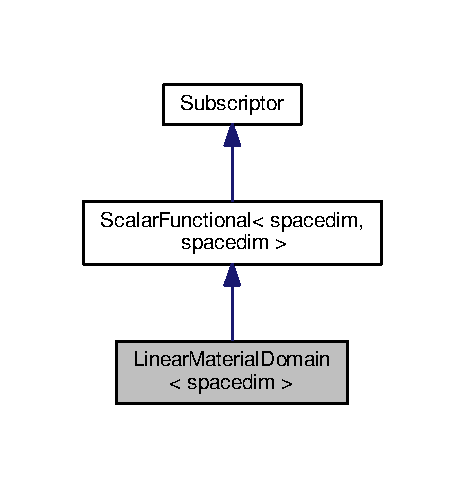
\includegraphics[width=238pt]{class_linear_material_domain__inherit__graph}
\end{center}
\end{figure}


Collaboration diagram for Linear\+Material\+Domain$<$ spacedim $>$\+:\nopagebreak
\begin{figure}[H]
\begin{center}
\leavevmode
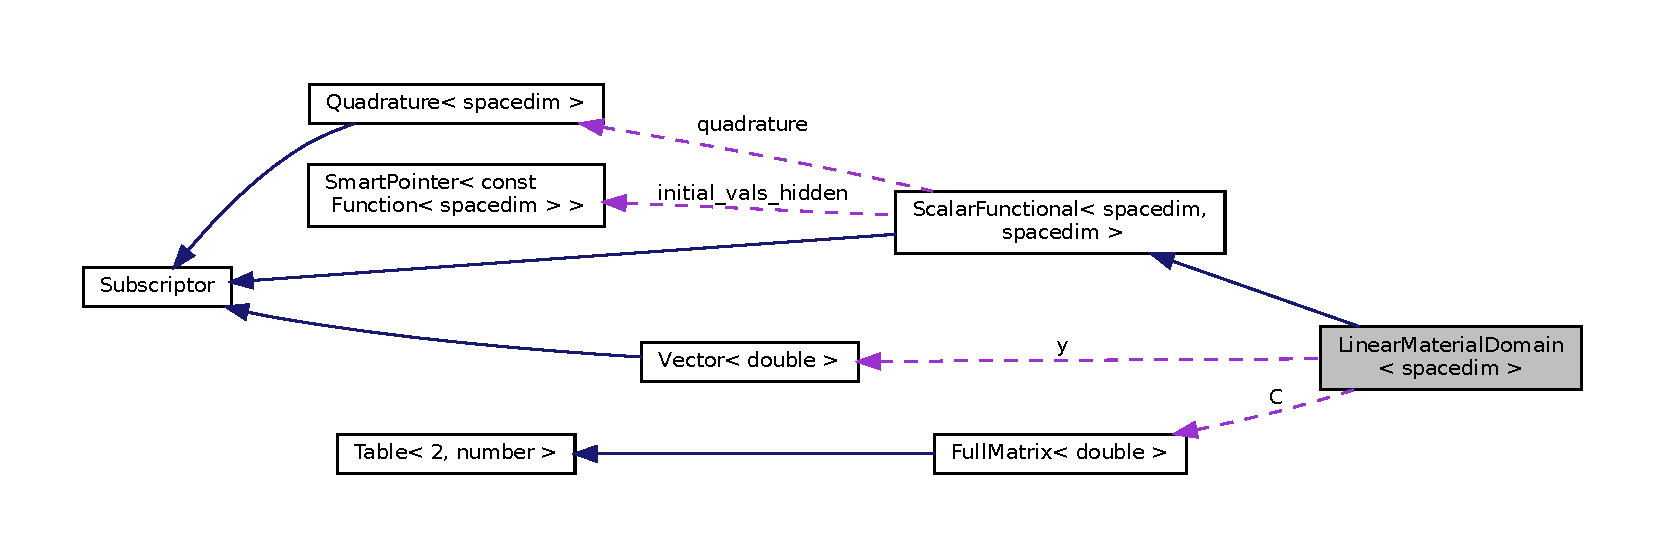
\includegraphics[width=350pt]{class_linear_material_domain__coll__graph}
\end{center}
\end{figure}
\doxysubsection*{Public Member Functions}
\begin{DoxyCompactItemize}
\item 
\mbox{\hyperlink{class_linear_material_domain_a7f91a980e9475691513443cd6b2efbc1}{Linear\+Material\+Domain}} (const \textbf{ std\+::vector}$<$ \mbox{\hyperlink{class_dependent_field}{Dependent\+Field}}$<$ spacedim, spacedim $>$$>$ \mbox{\hyperlink{class_scalar_functional_3_01spacedim_00_01spacedim_01_4_adfed9b70b743ba245a39c3e63b951f96}{e\+\_\+omega}}, const \textbf{ std\+::set}$<$ \textbf{ types\+::material\+\_\+id} $>$ \mbox{\hyperlink{class_scalar_functional_3_01spacedim_00_01spacedim_01_4_aa192395f822a64f60df43bf9d36c2f3a}{domain\+\_\+of\+\_\+integration}}, const \textbf{ Quadrature}$<$ spacedim $>$ \mbox{\hyperlink{class_scalar_functional_3_01spacedim_00_01spacedim_01_4_ab83ee3ae077b211137824b006098382e}{quadrature}}, const \textbf{ Full\+Matrix}$<$ double $>$ \mbox{\hyperlink{class_linear_material_domain_a8ac95fcf4f77790670b8520ba9593a7c}{C}}, const \textbf{ Vector}$<$ double $>$ \mbox{\hyperlink{class_linear_material_domain_a7ea9ab6930c0b0aa826e809ef245b0e2}{y}}, const std\+::string \mbox{\hyperlink{class_scalar_functional_3_01spacedim_00_01spacedim_01_4_a195248af3821548af3000872e9e6d00e}{name}}=\char`\"{}Linear\+Material\+Domain\char`\"{})
\item 
bool \mbox{\hyperlink{class_linear_material_domain_a4d73bbb0e545ee21c5635e7dac071719}{get\+\_\+h\+\_\+omega}} (\textbf{ Vector}$<$ double $>$ \&\mbox{\hyperlink{class_scalar_functional_3_01spacedim_00_01spacedim_01_4_adfed9b70b743ba245a39c3e63b951f96}{e\+\_\+omega}}, const \textbf{ std\+::vector}$<$ \textbf{ Vector}$<$ double $>$$>$ \&e\+\_\+omega\+\_\+ref\+\_\+sets, \textbf{ Vector}$<$ double $>$ \&hidden\+\_\+vars, const \textbf{ Point}$<$ spacedim $>$ \&x, double \&h\+\_\+omega, \textbf{ Vector}$<$ double $>$ \&h\+\_\+omega\+\_\+1, \textbf{ Full\+Matrix}$<$ double $>$ \&h\+\_\+omega\+\_\+2, const std\+::tuple$<$ bool, bool, bool $>$ requested\+\_\+quantities) const
\end{DoxyCompactItemize}
\doxysubsection*{Private Attributes}
\begin{DoxyCompactItemize}
\item 
const \textbf{ Full\+Matrix}$<$ double $>$ \mbox{\hyperlink{class_linear_material_domain_a8ac95fcf4f77790670b8520ba9593a7c}{C}}
\item 
const \textbf{ Vector}$<$ double $>$ \mbox{\hyperlink{class_linear_material_domain_a7ea9ab6930c0b0aa826e809ef245b0e2}{y}}
\end{DoxyCompactItemize}
\doxysubsection*{Additional Inherited Members}


\doxysubsection{Detailed Description}
\subsubsection*{template$<$unsigned int spacedim$>$\newline
class Linear\+Material\+Domain$<$ spacedim $>$}

Class defining the scalar functional $H^\Omega_\rho$ according to $H^\Omega_\rho=\int_\Omega \left[ \dfrac{1}{2} {\boldsymbol{e}^\Omega}^\top \boldsymbol{C} {\boldsymbol{e}^\Omega} + \boldsymbol{y}^\top \boldsymbol{e}^\Omega \right] \mathrm{d}V$, where $\boldsymbol{e}^\Omega$ is a vector with a selection of dependent fields $e^\Omega_\lambda$, $\boldsymbol{C}$ is a matrix, and $\boldsymbol{y}$ is a vector. 

\doxysubsection{Constructor \& Destructor Documentation}
\mbox{\Hypertarget{class_linear_material_domain_a7f91a980e9475691513443cd6b2efbc1}\label{class_linear_material_domain_a7f91a980e9475691513443cd6b2efbc1}} 
\index{LinearMaterialDomain$<$ spacedim $>$@{LinearMaterialDomain$<$ spacedim $>$}!LinearMaterialDomain@{LinearMaterialDomain}}
\index{LinearMaterialDomain@{LinearMaterialDomain}!LinearMaterialDomain$<$ spacedim $>$@{LinearMaterialDomain$<$ spacedim $>$}}
\doxysubsubsection{\texorpdfstring{LinearMaterialDomain()}{LinearMaterialDomain()}}
{\footnotesize\ttfamily template$<$unsigned int spacedim$>$ \\
\mbox{\hyperlink{class_linear_material_domain}{Linear\+Material\+Domain}}$<$ spacedim $>$\+::\mbox{\hyperlink{class_linear_material_domain}{Linear\+Material\+Domain}} (\begin{DoxyParamCaption}\item[{const \textbf{ std\+::vector}$<$ \mbox{\hyperlink{class_dependent_field}{Dependent\+Field}}$<$ spacedim, spacedim $>$$>$}]{e\+\_\+omega,  }\item[{const \textbf{ std\+::set}$<$ \textbf{ types\+::material\+\_\+id} $>$}]{domain\+\_\+of\+\_\+integration,  }\item[{const \textbf{ Quadrature}$<$ spacedim $>$}]{quadrature,  }\item[{const \textbf{ Full\+Matrix}$<$ double $>$}]{C,  }\item[{const \textbf{ Vector}$<$ double $>$}]{y,  }\item[{const std\+::string}]{name = {\ttfamily \char`\"{}LinearMaterialDomain$<$~spacedim~$>$\char`\"{}} }\end{DoxyParamCaption})}

The constructor of the class.


\begin{DoxyParams}[1]{Parameters}
\mbox{\texttt{ in}}  & {\em e\+\_\+omega} & \mbox{\hyperlink{class_scalar_functional_3_01spacedim_00_01spacedim_01_4_adfed9b70b743ba245a39c3e63b951f96}{Scalar\+Functional$<$spacedim, spacedim$>$\+::e\+\_\+omega}}\\
\hline
\mbox{\texttt{ in}}  & {\em domain\+\_\+of\+\_\+integration} & \mbox{\hyperlink{class_scalar_functional_3_01spacedim_00_01spacedim_01_4_aa192395f822a64f60df43bf9d36c2f3a}{Scalar\+Functional$<$spacedim, spacedim$>$\+::domain\+\_\+of\+\_\+integration}}\\
\hline
\mbox{\texttt{ in}}  & {\em quadrature} & \mbox{\hyperlink{class_scalar_functional_3_01spacedim_00_01spacedim_01_4_ab83ee3ae077b211137824b006098382e}{Scalar\+Functional$<$spacedim, spacedim$>$\+::quadrature}}\\
\hline
\mbox{\texttt{ in}}  & {\em C} & \mbox{\hyperlink{class_linear_material_domain_a8ac95fcf4f77790670b8520ba9593a7c}{Linear\+Material\+Domain\+::C}}\\
\hline
\mbox{\texttt{ in}}  & {\em y} & \mbox{\hyperlink{class_linear_material_domain_a7ea9ab6930c0b0aa826e809ef245b0e2}{Linear\+Material\+Domain\+::y}}\\
\hline
\mbox{\texttt{ in}}  & {\em name} & \mbox{\hyperlink{class_scalar_functional_3_01spacedim_00_01spacedim_01_4_a195248af3821548af3000872e9e6d00e}{Scalar\+Functional$<$spacedim, spacedim$>$\+::name}} \\
\hline
\end{DoxyParams}


\doxysubsection{Member Function Documentation}
\mbox{\Hypertarget{class_linear_material_domain_a4d73bbb0e545ee21c5635e7dac071719}\label{class_linear_material_domain_a4d73bbb0e545ee21c5635e7dac071719}} 
\index{LinearMaterialDomain$<$ spacedim $>$@{LinearMaterialDomain$<$ spacedim $>$}!get\_h\_omega@{get\_h\_omega}}
\index{get\_h\_omega@{get\_h\_omega}!LinearMaterialDomain$<$ spacedim $>$@{LinearMaterialDomain$<$ spacedim $>$}}
\doxysubsubsection{\texorpdfstring{get\_h\_omega()}{get\_h\_omega()}}
{\footnotesize\ttfamily template$<$unsigned int spacedim$>$ \\
bool \mbox{\hyperlink{class_linear_material_domain}{Linear\+Material\+Domain}}$<$ spacedim $>$\+::get\+\_\+h\+\_\+omega (\begin{DoxyParamCaption}\item[{\textbf{ Vector}$<$ double $>$ \&}]{e\+\_\+omega,  }\item[{const \textbf{ std\+::vector}$<$ \textbf{ Vector}$<$ double $>$$>$ \&}]{e\+\_\+omega\+\_\+ref\+\_\+sets,  }\item[{\textbf{ Vector}$<$ double $>$ \&}]{hidden\+\_\+vars,  }\item[{const \textbf{ Point}$<$ spacedim $>$ \&}]{x,  }\item[{double \&}]{h\+\_\+omega,  }\item[{\textbf{ Vector}$<$ double $>$ \&}]{h\+\_\+omega\+\_\+1,  }\item[{\textbf{ Full\+Matrix}$<$ double $>$ \&}]{h\+\_\+omega\+\_\+2,  }\item[{const std\+::tuple$<$ bool, bool, bool $>$}]{requested\+\_\+quantities }\end{DoxyParamCaption}) const\hspace{0.3cm}{\ttfamily [virtual]}}

See \mbox{\hyperlink{class_scalar_functional_3_01spacedim_00_01spacedim_01_4_a8665cb5b5a57ad22217e4c112845d43b}{Scalar\+Functional$<$spacedim, spacedim$>$\+::get\+\_\+h\+\_\+omega}} for detailed information on this method.


\begin{DoxyParams}[1]{Parameters}
\mbox{\texttt{ in}}  & {\em e\+\_\+omega} & $\boldsymbol{e}^\Omega$\\
\hline
\mbox{\texttt{ in}}  & {\em e\+\_\+omega\+\_\+ref\+\_\+sets} & Sets of reference values of $\boldsymbol{e}^\Omega$. None are required here.\\
\hline
\mbox{\texttt{ in,out}}  & {\em hidden\+\_\+vars} & Values of \char`\"{}hidden\char`\"{} variables associated with the integrand $h^\Omega_\rho$. Here, no hidden variables are present.\\
\hline
\mbox{\texttt{ in}}  & {\em x} & Location of material point\\
\hline
\mbox{\texttt{ out}}  & {\em h\+\_\+omega} & $\dfrac{1}{2} {\boldsymbol{e}^\Omega}^\top \boldsymbol{C} {\boldsymbol{e}^\Omega} + \boldsymbol{y}^\top \boldsymbol{e}^\Omega$\\
\hline
\mbox{\texttt{ out}}  & {\em h\+\_\+omega\+\_\+1} & $\boldsymbol{C} {\boldsymbol{e}^\Omega} + \boldsymbol{y}^\top$\\
\hline
\mbox{\texttt{ out}}  & {\em h\+\_\+omega\+\_\+2} & $\boldsymbol{C}$\\
\hline
\mbox{\texttt{ in}}  & {\em requested\+\_\+quantities} & A tuple indicating which quantities are actually to be computed\\
\hline
\end{DoxyParams}
\begin{DoxyReturn}{Returns}
{\ttfamily false} if the evaluation of {\ttfamily h\+\_\+omega}, {\ttfamily h\+\_\+omega\+\_\+1}, and {\ttfamily h\+\_\+omega\+\_\+2} was successful, and {\ttfamily true} if an error prevented the proper calculation of these quantities 
\end{DoxyReturn}


Implements \mbox{\hyperlink{class_scalar_functional_3_01spacedim_00_01spacedim_01_4_a8665cb5b5a57ad22217e4c112845d43b}{Scalar\+Functional$<$ spacedim, spacedim $>$}}.



\doxysubsection{Member Data Documentation}
\mbox{\Hypertarget{class_linear_material_domain_a8ac95fcf4f77790670b8520ba9593a7c}\label{class_linear_material_domain_a8ac95fcf4f77790670b8520ba9593a7c}} 
\index{LinearMaterialDomain$<$ spacedim $>$@{LinearMaterialDomain$<$ spacedim $>$}!C@{C}}
\index{C@{C}!LinearMaterialDomain$<$ spacedim $>$@{LinearMaterialDomain$<$ spacedim $>$}}
\doxysubsubsection{\texorpdfstring{C}{C}}
{\footnotesize\ttfamily template$<$unsigned int spacedim$>$ \\
const \textbf{ Full\+Matrix}$<$double$>$ \mbox{\hyperlink{class_linear_material_domain}{Linear\+Material\+Domain}}$<$ spacedim $>$\+::C\hspace{0.3cm}{\ttfamily [private]}}

$\boldsymbol{C}$ \mbox{\Hypertarget{class_linear_material_domain_a7ea9ab6930c0b0aa826e809ef245b0e2}\label{class_linear_material_domain_a7ea9ab6930c0b0aa826e809ef245b0e2}} 
\index{LinearMaterialDomain$<$ spacedim $>$@{LinearMaterialDomain$<$ spacedim $>$}!y@{y}}
\index{y@{y}!LinearMaterialDomain$<$ spacedim $>$@{LinearMaterialDomain$<$ spacedim $>$}}
\doxysubsubsection{\texorpdfstring{y}{y}}
{\footnotesize\ttfamily template$<$unsigned int spacedim$>$ \\
const \textbf{ Vector}$<$double$>$ \mbox{\hyperlink{class_linear_material_domain}{Linear\+Material\+Domain}}$<$ spacedim $>$\+::y\hspace{0.3cm}{\ttfamily [private]}}

$\boldsymbol{y}$ 

The documentation for this class was generated from the following file\+:\begin{DoxyCompactItemize}
\item 
/home/sst/code/\+Galerkin\+Tools/\+Galerkin\+Tools/include/galerkin\+\_\+tools/\mbox{\hyperlink{linear__material_8h}{linear\+\_\+material.\+h}}\end{DoxyCompactItemize}

\hypertarget{class_linear_material_interface}{}\doxysection{Linear\+Material\+Interface$<$ spacedim $>$ Class Template Reference}
\label{class_linear_material_interface}\index{LinearMaterialInterface$<$ spacedim $>$@{LinearMaterialInterface$<$ spacedim $>$}}


{\ttfamily \#include $<$linear\+\_\+material.\+h$>$}



Inheritance diagram for Linear\+Material\+Interface$<$ spacedim $>$\+:\nopagebreak
\begin{figure}[H]
\begin{center}
\leavevmode
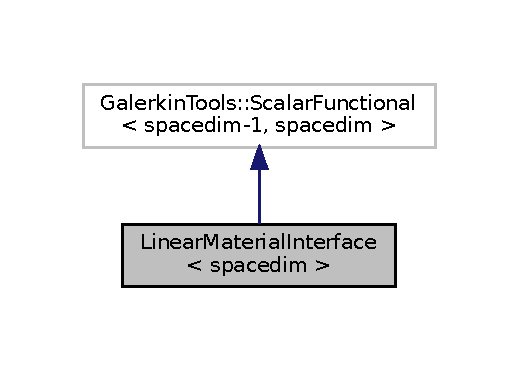
\includegraphics[width=249pt]{class_linear_material_interface__inherit__graph}
\end{center}
\end{figure}


Collaboration diagram for Linear\+Material\+Interface$<$ spacedim $>$\+:\nopagebreak
\begin{figure}[H]
\begin{center}
\leavevmode
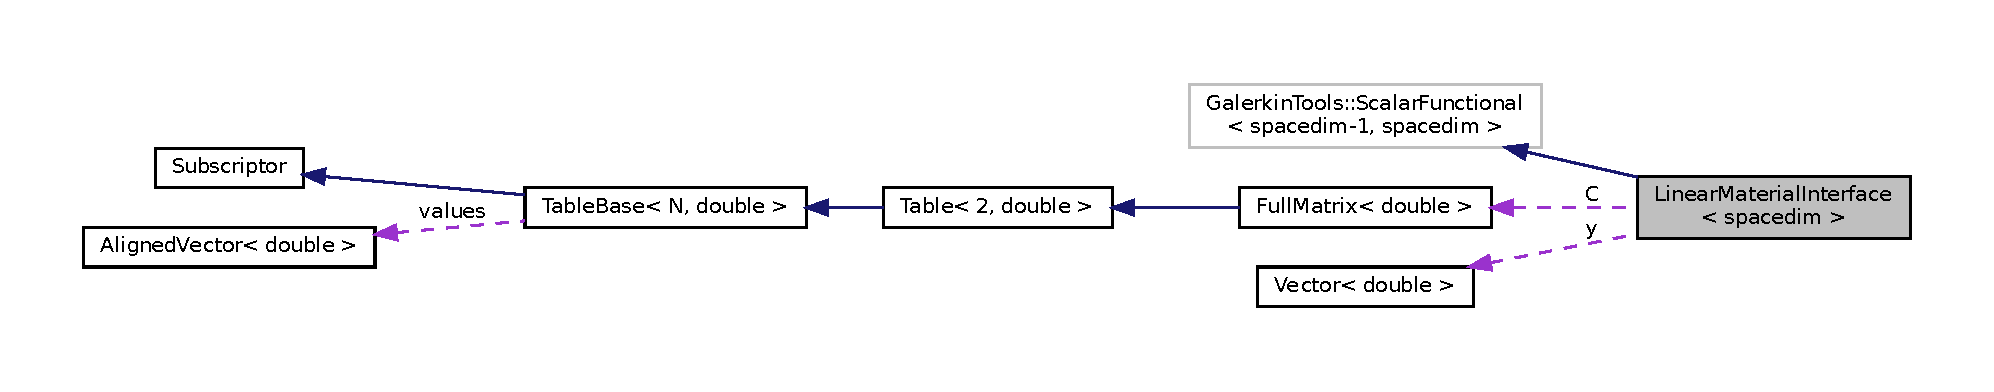
\includegraphics[width=350pt]{class_linear_material_interface__coll__graph}
\end{center}
\end{figure}
\doxysubsection*{Public Member Functions}
\begin{DoxyCompactItemize}
\item 
\mbox{\hyperlink{class_linear_material_interface_ac10a5c148dd81edab41d22dd207c78a2}{Linear\+Material\+Interface}} (const \textbf{ std\+::vector}$<$ \mbox{\hyperlink{class_dependent_field}{Dependent\+Field}}$<$ spacedim-\/1, spacedim $>$$>$ e\+\_\+sigma, const \textbf{ std\+::set}$<$ \textbf{ types\+::material\+\_\+id} $>$ domain\+\_\+of\+\_\+integration, const \textbf{ Quadrature}$<$ spacedim-\/1 $>$ quadrature, const \textbf{ Full\+Matrix}$<$ double $>$ \mbox{\hyperlink{class_linear_material_interface_ae0b1ef211453e5fd3e1416ff37c315db}{C}}, const \textbf{ Vector}$<$ double $>$ \mbox{\hyperlink{class_linear_material_interface_a3864513d7662e4d1c91e606467befd59}{y}}, const std\+::string name=\char`\"{}Linear\+Material\+Interface\char`\"{})
\item 
bool \mbox{\hyperlink{class_linear_material_interface_af5cca6ebef9371fd07782e3ae0171d65}{get\+\_\+h\+\_\+sigma}} (\textbf{ Vector}$<$ double $>$ \&e\+\_\+sigma, const \textbf{ std\+::vector}$<$ \textbf{ Vector}$<$ double $>$$>$ \&e\+\_\+sigma\+\_\+ref\+\_\+sets, \textbf{ Vector}$<$ double $>$ \&hidden\+\_\+vars, const \textbf{ Point}$<$ spacedim $>$ \&x, const \textbf{ Tensor}$<$ 1, spacedim $>$ \&\textbf{ n}, double \&h\+\_\+sigma, \textbf{ Vector}$<$ double $>$ \&h\+\_\+sigma\+\_\+1, \textbf{ Full\+Matrix}$<$ double $>$ \&h\+\_\+sigma\+\_\+2, const std\+::tuple$<$ bool, bool, bool $>$ requested\+\_\+quantities) const
\end{DoxyCompactItemize}
\doxysubsection*{Private Attributes}
\begin{DoxyCompactItemize}
\item 
const \textbf{ Full\+Matrix}$<$ double $>$ \mbox{\hyperlink{class_linear_material_interface_ae0b1ef211453e5fd3e1416ff37c315db}{C}}
\item 
const \textbf{ Vector}$<$ double $>$ \mbox{\hyperlink{class_linear_material_interface_a3864513d7662e4d1c91e606467befd59}{y}}
\end{DoxyCompactItemize}


\doxysubsection{Detailed Description}
\subsubsection*{template$<$unsigned int spacedim$>$\newline
class Linear\+Material\+Interface$<$ spacedim $>$}

Class defining the scalar functional $H^\Sigma_\tau$ according to $H^\Sigma_\tau=\int_\Sigma \left[ \dfrac{1}{2} {\boldsymbol{e}^\Sigma}^\top \boldsymbol{C} {\boldsymbol{e}^\Sigma} + \boldsymbol{y}^\top \boldsymbol{e}^\Sigma \right] \mathrm{d}S$, where $\boldsymbol{e}^\Sigma$ is a vector with a selection of dependent fields $e^\Sigma_\nu$, $\boldsymbol{C}$ is a matrix, and $\boldsymbol{y}$ is a vector. 

\doxysubsection{Constructor \& Destructor Documentation}
\mbox{\Hypertarget{class_linear_material_interface_ac10a5c148dd81edab41d22dd207c78a2}\label{class_linear_material_interface_ac10a5c148dd81edab41d22dd207c78a2}} 
\index{LinearMaterialInterface$<$ spacedim $>$@{LinearMaterialInterface$<$ spacedim $>$}!LinearMaterialInterface@{LinearMaterialInterface}}
\index{LinearMaterialInterface@{LinearMaterialInterface}!LinearMaterialInterface$<$ spacedim $>$@{LinearMaterialInterface$<$ spacedim $>$}}
\doxysubsubsection{\texorpdfstring{LinearMaterialInterface()}{LinearMaterialInterface()}}
{\footnotesize\ttfamily template$<$unsigned int spacedim$>$ \\
\mbox{\hyperlink{class_linear_material_interface}{Linear\+Material\+Interface}}$<$ spacedim $>$\+::\mbox{\hyperlink{class_linear_material_interface}{Linear\+Material\+Interface}} (\begin{DoxyParamCaption}\item[{const \textbf{ std\+::vector}$<$ \mbox{\hyperlink{class_dependent_field}{Dependent\+Field}}$<$ spacedim-\/1, spacedim $>$$>$}]{e\+\_\+sigma,  }\item[{const \textbf{ std\+::set}$<$ \textbf{ types\+::material\+\_\+id} $>$}]{domain\+\_\+of\+\_\+integration,  }\item[{const \textbf{ Quadrature}$<$ spacedim-\/1 $>$}]{quadrature,  }\item[{const \textbf{ Full\+Matrix}$<$ double $>$}]{C,  }\item[{const \textbf{ Vector}$<$ double $>$}]{y,  }\item[{const std\+::string}]{name = {\ttfamily \char`\"{}LinearMaterialInterface$<$~spacedim~$>$\char`\"{}} }\end{DoxyParamCaption})}

The constructor of the class.


\begin{DoxyParams}[1]{Parameters}
\mbox{\texttt{ in}}  & {\em e\+\_\+sigma} & \mbox{\hyperlink{class_scalar_functional_a86662b03a63219227993a2c6c07aefc1}{Scalar\+Functional\+::e\+\_\+sigma}}\\
\hline
\mbox{\texttt{ in}}  & {\em domain\+\_\+of\+\_\+integration} & \mbox{\hyperlink{class_scalar_functional_ae3b6dd6934e1cd55fcc55cf344179407}{Scalar\+Functional\+::domain\+\_\+of\+\_\+integration}}\\
\hline
\mbox{\texttt{ in}}  & {\em quadrature} & \mbox{\hyperlink{class_scalar_functional_adea9ff214aeb2a1d8c3712a9d2433883}{Scalar\+Functional\+::quadrature}}\\
\hline
\mbox{\texttt{ in}}  & {\em C} & \mbox{\hyperlink{class_linear_material_interface_ae0b1ef211453e5fd3e1416ff37c315db}{Linear\+Material\+Interface\+::C}}\\
\hline
\mbox{\texttt{ in}}  & {\em y} & \mbox{\hyperlink{class_linear_material_interface_a3864513d7662e4d1c91e606467befd59}{Linear\+Material\+Interface\+::y}}\\
\hline
\mbox{\texttt{ in}}  & {\em name} & \mbox{\hyperlink{class_scalar_functional_a4d184688053b3443d10e228e4a8eba60}{Scalar\+Functional\+::name}} \\
\hline
\end{DoxyParams}


\doxysubsection{Member Function Documentation}
\mbox{\Hypertarget{class_linear_material_interface_af5cca6ebef9371fd07782e3ae0171d65}\label{class_linear_material_interface_af5cca6ebef9371fd07782e3ae0171d65}} 
\index{LinearMaterialInterface$<$ spacedim $>$@{LinearMaterialInterface$<$ spacedim $>$}!get\_h\_sigma@{get\_h\_sigma}}
\index{get\_h\_sigma@{get\_h\_sigma}!LinearMaterialInterface$<$ spacedim $>$@{LinearMaterialInterface$<$ spacedim $>$}}
\doxysubsubsection{\texorpdfstring{get\_h\_sigma()}{get\_h\_sigma()}}
{\footnotesize\ttfamily template$<$unsigned int spacedim$>$ \\
bool \mbox{\hyperlink{class_linear_material_interface}{Linear\+Material\+Interface}}$<$ spacedim $>$\+::get\+\_\+h\+\_\+sigma (\begin{DoxyParamCaption}\item[{\textbf{ Vector}$<$ double $>$ \&}]{e\+\_\+sigma,  }\item[{const \textbf{ std\+::vector}$<$ \textbf{ Vector}$<$ double $>$$>$ \&}]{e\+\_\+sigma\+\_\+ref\+\_\+sets,  }\item[{\textbf{ Vector}$<$ double $>$ \&}]{hidden\+\_\+vars,  }\item[{const \textbf{ Point}$<$ spacedim $>$ \&}]{x,  }\item[{const \textbf{ Tensor}$<$ 1, spacedim $>$ \&}]{n,  }\item[{double \&}]{h\+\_\+sigma,  }\item[{\textbf{ Vector}$<$ double $>$ \&}]{h\+\_\+sigma\+\_\+1,  }\item[{\textbf{ Full\+Matrix}$<$ double $>$ \&}]{h\+\_\+sigma\+\_\+2,  }\item[{const std\+::tuple$<$ bool, bool, bool $>$}]{requested\+\_\+quantities }\end{DoxyParamCaption}) const}

See \mbox{\hyperlink{class_scalar_functional_adb295fb739a743d5a1273025eb8dae72}{Scalar\+Functional\+::get\+\_\+h\+\_\+sigma}} for detailed information on this method.


\begin{DoxyParams}[1]{Parameters}
\mbox{\texttt{ in}}  & {\em e\+\_\+sigma} & $\boldsymbol{e}^\Sigma$\\
\hline
\mbox{\texttt{ in}}  & {\em e\+\_\+sigma\+\_\+ref\+\_\+sets} & Sets of reference values of $\boldsymbol{e}^\Sigma$. None are required here.\\
\hline
\mbox{\texttt{ in,out}}  & {\em hidden\+\_\+vars} & Values of \char`\"{}hidden\char`\"{} variables associated with the integrand $h^\Sigma_\tau$. Here, no hidden variables are present.\\
\hline
\mbox{\texttt{ in}}  & {\em x} & Location of material point\\
\hline
\mbox{\texttt{ in}}  & {\em n} & Normal vector pointing from -\/ to + side of the interface $\Sigma$ at {\ttfamily x}. Not required for this particular scalar functional.\\
\hline
\mbox{\texttt{ out}}  & {\em h\+\_\+sigma} & $\dfrac{1}{2} {\boldsymbol{e}^\Sigma}^\top \boldsymbol{C} {\boldsymbol{e}^\Sigma} + \boldsymbol{y}^\top \boldsymbol{e}^\Sigma$\\
\hline
\mbox{\texttt{ out}}  & {\em h\+\_\+sigma\+\_\+1} & $\boldsymbol{C} {\boldsymbol{e}^\Sigma} + \boldsymbol{y}^\top$\\
\hline
\mbox{\texttt{ out}}  & {\em h\+\_\+sigma\+\_\+2} & $\boldsymbol{C}$\\
\hline
\mbox{\texttt{ in}}  & {\em requested\+\_\+quantities} & A tuple indicating which quantities are actually to be computed\\
\hline
\end{DoxyParams}
\begin{DoxyReturn}{Returns}
{\ttfamily false} if the evaluation of {\ttfamily h\+\_\+sigma}, {\ttfamily h\+\_\+sigma\+\_\+1}, and {\ttfamily h\+\_\+sigma\+\_\+2} was successful, and {\ttfamily true} if an error prevented the proper calculation of these quantities 
\end{DoxyReturn}


\doxysubsection{Member Data Documentation}
\mbox{\Hypertarget{class_linear_material_interface_ae0b1ef211453e5fd3e1416ff37c315db}\label{class_linear_material_interface_ae0b1ef211453e5fd3e1416ff37c315db}} 
\index{LinearMaterialInterface$<$ spacedim $>$@{LinearMaterialInterface$<$ spacedim $>$}!C@{C}}
\index{C@{C}!LinearMaterialInterface$<$ spacedim $>$@{LinearMaterialInterface$<$ spacedim $>$}}
\doxysubsubsection{\texorpdfstring{C}{C}}
{\footnotesize\ttfamily template$<$unsigned int spacedim$>$ \\
const \textbf{ Full\+Matrix}$<$double$>$ \mbox{\hyperlink{class_linear_material_interface}{Linear\+Material\+Interface}}$<$ spacedim $>$\+::C\hspace{0.3cm}{\ttfamily [private]}}

$\boldsymbol{C}$ \mbox{\Hypertarget{class_linear_material_interface_a3864513d7662e4d1c91e606467befd59}\label{class_linear_material_interface_a3864513d7662e4d1c91e606467befd59}} 
\index{LinearMaterialInterface$<$ spacedim $>$@{LinearMaterialInterface$<$ spacedim $>$}!y@{y}}
\index{y@{y}!LinearMaterialInterface$<$ spacedim $>$@{LinearMaterialInterface$<$ spacedim $>$}}
\doxysubsubsection{\texorpdfstring{y}{y}}
{\footnotesize\ttfamily template$<$unsigned int spacedim$>$ \\
const \textbf{ Vector}$<$double$>$ \mbox{\hyperlink{class_linear_material_interface}{Linear\+Material\+Interface}}$<$ spacedim $>$\+::y\hspace{0.3cm}{\ttfamily [private]}}

$\boldsymbol{y}$ 

The documentation for this class was generated from the following file\+:\begin{DoxyCompactItemize}
\item 
/home/sst/code/\+Galerkin\+Tools/\+Galerkin\+Tools/include/galerkin\+\_\+tools/\mbox{\hyperlink{linear__material_8h}{linear\+\_\+material.\+h}}\end{DoxyCompactItemize}

\hypertarget{class_scalar_functional}{}\doxysection{Scalar\+Functional$<$ dim, spacedim $>$ Class Template Reference}
\label{class_scalar_functional}\index{ScalarFunctional$<$ dim, spacedim $>$@{ScalarFunctional$<$ dim, spacedim $>$}}


{\ttfamily \#include $<$scalar\+\_\+functional.\+h$>$}



Inheritance diagram for Scalar\+Functional$<$ dim, spacedim $>$\+:\nopagebreak
\begin{figure}[H]
\begin{center}
\leavevmode
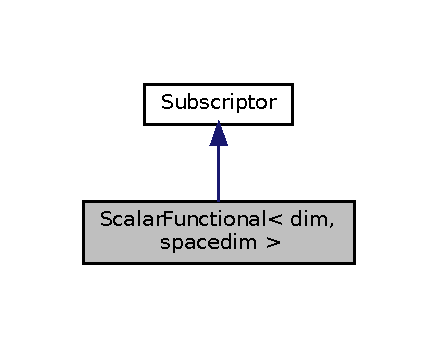
\includegraphics[width=210pt]{class_scalar_functional__inherit__graph}
\end{center}
\end{figure}


Collaboration diagram for Scalar\+Functional$<$ dim, spacedim $>$\+:\nopagebreak
\begin{figure}[H]
\begin{center}
\leavevmode
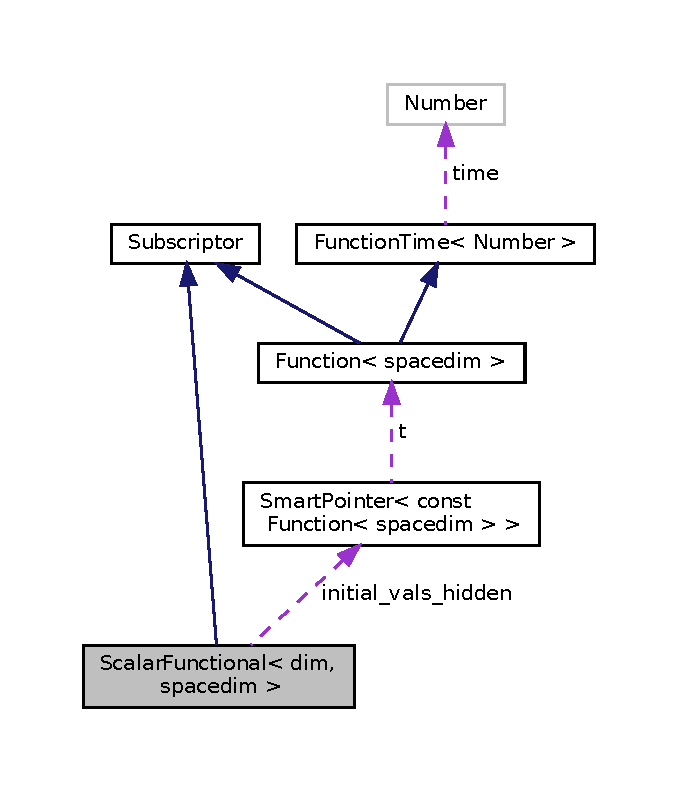
\includegraphics[width=326pt]{class_scalar_functional__coll__graph}
\end{center}
\end{figure}
\doxysubsection*{Public Member Functions}
\begin{DoxyCompactItemize}
\item 
\mbox{\hyperlink{class_scalar_functional_ac0618ada3b80400784ee8553a66aade9}{Scalar\+Functional}} (const std\+::vector$<$ \mbox{\hyperlink{class_dependent_field}{Dependent\+Field}}$<$ dim, spacedim $>$$>$ \mbox{\hyperlink{class_scalar_functional_a86662b03a63219227993a2c6c07aefc1}{e\+\_\+sigma}}, const std\+::set$<$ \textbf{ types\+::material\+\_\+id} $>$ \mbox{\hyperlink{class_scalar_functional_ae3b6dd6934e1cd55fcc55cf344179407}{domain\+\_\+of\+\_\+integration}}, const \textbf{ Quadrature}$<$ dim $>$ \mbox{\hyperlink{class_scalar_functional_adea9ff214aeb2a1d8c3712a9d2433883}{quadrature}}, const std\+::string \mbox{\hyperlink{class_scalar_functional_a4d184688053b3443d10e228e4a8eba60}{name}}, const unsigned int \mbox{\hyperlink{class_scalar_functional_a7e12423f4b29e9e0aaa0f7f9c2d1c0eb}{n\+\_\+ref\+\_\+sets}}=0, const unsigned int \mbox{\hyperlink{class_scalar_functional_a8b1617930242870f22eef5e306cb717f}{n\+\_\+hidden}}=0, const \textbf{ Function}$<$ spacedim $>$ $\ast$const \mbox{\hyperlink{class_scalar_functional_a602d0bc2c945822c6b756fc63183ae2b}{initial\+\_\+vals\+\_\+hidden}}=nullptr)
\item 
virtual bool \mbox{\hyperlink{class_scalar_functional_a1b9874b2fd591c844ecfcd1db8212c54}{get\+\_\+h\+\_\+sigma}} (const \textbf{ Vector}$<$ double $>$ \&\mbox{\hyperlink{class_scalar_functional_a86662b03a63219227993a2c6c07aefc1}{e\+\_\+sigma}}, const std\+::vector$<$ \textbf{ Vector}$<$ double $>$$>$ \&e\+\_\+sigma\+\_\+ref\+\_\+sets, \textbf{ Vector}$<$ double $>$ \&hidden\+\_\+vars, const \textbf{ Point}$<$ spacedim $>$ \&x, const \textbf{ Tensor}$<$ 1, spacedim $>$ \&n, double \&h\+\_\+sigma, \textbf{ Vector}$<$ double $>$ \&h\+\_\+sigma\+\_\+1, \textbf{ Full\+Matrix}$<$ double $>$ \&h\+\_\+sigma\+\_\+2, const std\+::tuple$<$ bool, bool, bool $>$ requested\+\_\+quantities) const =0
\item 
virtual double \mbox{\hyperlink{class_scalar_functional_ae4f5fbd69cabfda73cc2b30ae0263ca5}{get\+\_\+maximum\+\_\+step}} (const \textbf{ Vector}$<$ double $>$ \&\mbox{\hyperlink{class_scalar_functional_a86662b03a63219227993a2c6c07aefc1}{e\+\_\+sigma}}, const std\+::vector$<$ \textbf{ Vector}$<$ double $>$$>$ \&e\+\_\+sigma\+\_\+ref\+\_\+sets, const \textbf{ Vector}$<$ double $>$ \&delta\+\_\+e\+\_\+sigma, const \textbf{ Vector}$<$ double $>$ \&hidden\+\_\+vars, const \textbf{ Point}$<$ spacedim $>$ \&x, const \textbf{ Tensor}$<$ 1, spacedim $>$ \&n) const
\item 
void \mbox{\hyperlink{class_scalar_functional_a0c0a2095a33e657a7a984e706ed7f968}{compare\+\_\+derivatives\+\_\+with\+\_\+numerical\+\_\+derivatives}} (\textbf{ Vector}$<$ double $>$ \&\mbox{\hyperlink{class_scalar_functional_a86662b03a63219227993a2c6c07aefc1}{e\+\_\+sigma}}, const std\+::vector$<$ \textbf{ Vector}$<$ double $>$$>$ \&e\+\_\+sigma\+\_\+ref\+\_\+sets, \textbf{ Vector}$<$ double $>$ \&hidden\+\_\+vars, const \textbf{ Point}$<$ spacedim $>$ \&x, const \textbf{ Tensor}$<$ 1, spacedim $>$ \&n, const std\+::string detailed\+\_\+printout\+\_\+file=\char`\"{}\char`\"{}, const double \textbf{ epsilon}=1\textbf{ e}-\/8) const
\item 
virtual \mbox{\hyperlink{class_scalar_functional_aed36f35e6d2c9f9a93ee2749d01f2a51}{$\sim$\+Scalar\+Functional}} ()
\end{DoxyCompactItemize}
\doxysubsection*{Public Attributes}
\begin{DoxyCompactItemize}
\item 
const std\+::set$<$ \textbf{ types\+::material\+\_\+id} $>$ \mbox{\hyperlink{class_scalar_functional_ae3b6dd6934e1cd55fcc55cf344179407}{domain\+\_\+of\+\_\+integration}}
\item 
const \textbf{ Smart\+Pointer}$<$ const \textbf{ Function}$<$ spacedim $>$ $>$ \mbox{\hyperlink{class_scalar_functional_a602d0bc2c945822c6b756fc63183ae2b}{initial\+\_\+vals\+\_\+hidden}}
\item 
const std\+::vector$<$ \mbox{\hyperlink{class_dependent_field}{Dependent\+Field}}$<$ dim, spacedim $>$ $>$ \mbox{\hyperlink{class_scalar_functional_a86662b03a63219227993a2c6c07aefc1}{e\+\_\+sigma}}
\item 
const \textbf{ Quadrature}$<$ dim $>$ \mbox{\hyperlink{class_scalar_functional_adea9ff214aeb2a1d8c3712a9d2433883}{quadrature}}
\item 
const unsigned int \mbox{\hyperlink{class_scalar_functional_a8b1617930242870f22eef5e306cb717f}{n\+\_\+hidden}}
\item 
const std\+::string \mbox{\hyperlink{class_scalar_functional_a4d184688053b3443d10e228e4a8eba60}{name}}
\item 
const unsigned int \mbox{\hyperlink{class_scalar_functional_a7e12423f4b29e9e0aaa0f7f9c2d1c0eb}{n\+\_\+ref\+\_\+sets}}
\end{DoxyCompactItemize}
\doxysubsection*{Additional Inherited Members}


\doxysubsection{Detailed Description}
\subsubsection*{template$<$unsigned int dim, unsigned int spacedim$>$\newline
class Scalar\+Functional$<$ dim, spacedim $>$}

Class defining an interface related scalar functional $H^\Sigma_\tau = \int_\Sigma h^\Sigma_\tau(e^\Sigma_\nu, \boldsymbol{X}) \mathrm{d}S$, where $\tau \in T=\left\{1 \hdots N^\mathrm{H,\Sigma}\right\}$.

\char`\"{}\+Hidden\char`\"{} variables involved in the definition of the functions $h^\Sigma_\tau$ are allowed for (in order to allow for incorporation of e.\+g. classical plasticity formulations).

The integrand $h^\Sigma_\tau$ may, besides the current values of $e^\Sigma_\nu$, also depend on an arbitrary number of sets of \char`\"{}reference values\char`\"{} of $e^\Sigma_\nu$. These reference values can e.\+g. be the values of the $e^\Sigma_\nu$ at previous instants of time. When derivatives of $h^\Sigma_\tau$ w.\+r.\+t. the dependent variables are calculated, these reference values are generally regarded as fixed.

In principle, it is often sufficient that the first and second derivatives of $h^\Sigma_\tau$ are known, as the values themselves do not factor into the finite element system. However, this depends on the exact problem.

The \mbox{\hyperlink{class_scalar_functional}{Scalar\+Functional}} class inherits from \textbf{ Subscriptor} in order to be able to check that \mbox{\hyperlink{class_scalar_functional}{Scalar\+Functional}} objects are only destroyed when they are not needed anymore by other objects.


\begin{DoxyTemplParams}{Template Parameters}
{\em dim} & The dimension of the object on which the \mbox{\hyperlink{class_scalar_functional}{Scalar\+Functional}} is defined. Currently, only {\ttfamily dim} = {\ttfamily spacedim-\/1} is considered, although this class would in principle also work for scalar functionals on lower dimensional objects.\\
\hline
{\em spacedim} & The spatial dimension of the problem \\
\hline
\end{DoxyTemplParams}


\doxysubsection{Constructor \& Destructor Documentation}
\mbox{\Hypertarget{class_scalar_functional_ac0618ada3b80400784ee8553a66aade9}\label{class_scalar_functional_ac0618ada3b80400784ee8553a66aade9}} 
\index{ScalarFunctional$<$ dim, spacedim $>$@{ScalarFunctional$<$ dim, spacedim $>$}!ScalarFunctional@{ScalarFunctional}}
\index{ScalarFunctional@{ScalarFunctional}!ScalarFunctional$<$ dim, spacedim $>$@{ScalarFunctional$<$ dim, spacedim $>$}}
\doxysubsubsection{\texorpdfstring{ScalarFunctional()}{ScalarFunctional()}}
{\footnotesize\ttfamily template$<$unsigned int dim, unsigned int spacedim$>$ \\
\mbox{\hyperlink{class_scalar_functional}{Scalar\+Functional}}$<$ dim, spacedim $>$\+::\mbox{\hyperlink{class_scalar_functional}{Scalar\+Functional}} (\begin{DoxyParamCaption}\item[{const std\+::vector$<$ \mbox{\hyperlink{class_dependent_field}{Dependent\+Field}}$<$ dim, spacedim $>$$>$}]{e\+\_\+sigma,  }\item[{const std\+::set$<$ \textbf{ types\+::material\+\_\+id} $>$}]{domain\+\_\+of\+\_\+integration,  }\item[{const \textbf{ Quadrature}$<$ dim $>$}]{quadrature,  }\item[{const std\+::string}]{name,  }\item[{const unsigned int}]{n\+\_\+ref\+\_\+sets = {\ttfamily 0},  }\item[{const unsigned int}]{n\+\_\+hidden = {\ttfamily 0},  }\item[{const \textbf{ Function}$<$ spacedim $>$ $\ast$const}]{initial\+\_\+vals\+\_\+hidden = {\ttfamily nullptr} }\end{DoxyParamCaption})}

The constructor of the class


\begin{DoxyParams}[1]{Parameters}
\mbox{\texttt{ in}}  & {\em e\+\_\+sigma} & \mbox{\hyperlink{class_scalar_functional_a86662b03a63219227993a2c6c07aefc1}{Scalar\+Functional\+::e\+\_\+sigma}}\\
\hline
\mbox{\texttt{ in}}  & {\em domain\+\_\+of\+\_\+integration} & \mbox{\hyperlink{class_scalar_functional_ae3b6dd6934e1cd55fcc55cf344179407}{Scalar\+Functional\+::domain\+\_\+of\+\_\+integration}}\\
\hline
\mbox{\texttt{ in}}  & {\em quadrature} & \mbox{\hyperlink{class_scalar_functional_adea9ff214aeb2a1d8c3712a9d2433883}{Scalar\+Functional\+::quadrature}}\\
\hline
\mbox{\texttt{ in}}  & {\em name} & \mbox{\hyperlink{class_scalar_functional_a4d184688053b3443d10e228e4a8eba60}{Scalar\+Functional\+::name}}\\
\hline
\mbox{\texttt{ in}}  & {\em n\+\_\+ref\+\_\+sets} & \mbox{\hyperlink{class_scalar_functional_a7e12423f4b29e9e0aaa0f7f9c2d1c0eb}{Scalar\+Functional\+::n\+\_\+ref\+\_\+sets}}\\
\hline
\mbox{\texttt{ in}}  & {\em n\+\_\+hidden} & \mbox{\hyperlink{class_scalar_functional_a8b1617930242870f22eef5e306cb717f}{Scalar\+Functional\+::n\+\_\+hidden}}\\
\hline
\mbox{\texttt{ in}}  & {\em initial\+\_\+vals\+\_\+hidden} & \mbox{\hyperlink{class_scalar_functional_a602d0bc2c945822c6b756fc63183ae2b}{Scalar\+Functional\+::initial\+\_\+vals\+\_\+hidden}} (if {\ttfamily n\+\_\+hidden$>$0} and this argument is omitted, the initial values will be set to zero) \\
\hline
\end{DoxyParams}
\mbox{\Hypertarget{class_scalar_functional_aed36f35e6d2c9f9a93ee2749d01f2a51}\label{class_scalar_functional_aed36f35e6d2c9f9a93ee2749d01f2a51}} 
\index{ScalarFunctional$<$ dim, spacedim $>$@{ScalarFunctional$<$ dim, spacedim $>$}!````~ScalarFunctional@{$\sim$ScalarFunctional}}
\index{````~ScalarFunctional@{$\sim$ScalarFunctional}!ScalarFunctional$<$ dim, spacedim $>$@{ScalarFunctional$<$ dim, spacedim $>$}}
\doxysubsubsection{\texorpdfstring{$\sim$ScalarFunctional()}{~ScalarFunctional()}}
{\footnotesize\ttfamily template$<$unsigned int dim, unsigned int spacedim$>$ \\
virtual \mbox{\hyperlink{class_scalar_functional}{Scalar\+Functional}}$<$ dim, spacedim $>$\+::$\sim$\mbox{\hyperlink{class_scalar_functional}{Scalar\+Functional}} (\begin{DoxyParamCaption}{ }\end{DoxyParamCaption})\hspace{0.3cm}{\ttfamily [virtual]}}

The destructor of \mbox{\hyperlink{class_scalar_functional}{Scalar\+Functional}} essentially checks before destruction that the \mbox{\hyperlink{class_scalar_functional}{Scalar\+Functional}} object is not used by other objects. If this is the case, the program will be aborted. 

\doxysubsection{Member Function Documentation}
\mbox{\Hypertarget{class_scalar_functional_a0c0a2095a33e657a7a984e706ed7f968}\label{class_scalar_functional_a0c0a2095a33e657a7a984e706ed7f968}} 
\index{ScalarFunctional$<$ dim, spacedim $>$@{ScalarFunctional$<$ dim, spacedim $>$}!compare\_derivatives\_with\_numerical\_derivatives@{compare\_derivatives\_with\_numerical\_derivatives}}
\index{compare\_derivatives\_with\_numerical\_derivatives@{compare\_derivatives\_with\_numerical\_derivatives}!ScalarFunctional$<$ dim, spacedim $>$@{ScalarFunctional$<$ dim, spacedim $>$}}
\doxysubsubsection{\texorpdfstring{compare\_derivatives\_with\_numerical\_derivatives()}{compare\_derivatives\_with\_numerical\_derivatives()}}
{\footnotesize\ttfamily template$<$unsigned int dim, unsigned int spacedim$>$ \\
void \mbox{\hyperlink{class_scalar_functional}{Scalar\+Functional}}$<$ dim, spacedim $>$\+::compare\+\_\+derivatives\+\_\+with\+\_\+numerical\+\_\+derivatives (\begin{DoxyParamCaption}\item[{\textbf{ Vector}$<$ double $>$ \&}]{e\+\_\+sigma,  }\item[{const std\+::vector$<$ \textbf{ Vector}$<$ double $>$$>$ \&}]{e\+\_\+sigma\+\_\+ref\+\_\+sets,  }\item[{\textbf{ Vector}$<$ double $>$ \&}]{hidden\+\_\+vars,  }\item[{const \textbf{ Point}$<$ spacedim $>$ \&}]{x,  }\item[{const \textbf{ Tensor}$<$ 1, spacedim $>$ \&}]{n,  }\item[{const std\+::string}]{detailed\+\_\+printout\+\_\+file = {\ttfamily \char`\"{}\char`\"{}},  }\item[{const double}]{epsilon = {\ttfamily 1\textbf{ e}-\/8} }\end{DoxyParamCaption}) const}

Function comparing the computed derivatives of the integrand $h^\Sigma_\tau$ provided by \mbox{\hyperlink{class_scalar_functional_a1b9874b2fd591c844ecfcd1db8212c54}{Scalar\+Functional\+::get\+\_\+h\+\_\+sigma()}} with corresponding numerically computed finite difference based derivatives.

In the case of the first derivative, the numerical derivatives are obtained based on the values for $h^\Sigma_\tau$ provided by \mbox{\hyperlink{class_scalar_functional_a1b9874b2fd591c844ecfcd1db8212c54}{Scalar\+Functional\+::get\+\_\+h\+\_\+sigma()}}; and in the case of the second derivatives, the numerical derivatives are obtained based on the values for the first derivatives of $h^\Sigma_\tau$ provided by \mbox{\hyperlink{class_scalar_functional_a1b9874b2fd591c844ecfcd1db8212c54}{Scalar\+Functional\+::get\+\_\+h\+\_\+sigma()}} ). In both cases, a simple forward finite difference approach is used. Generally, the first numerical derivative can only be \char`\"{}correct\char`\"{} if the computation of the value of $h^\Sigma_\tau$ is correctly implemented in the function \mbox{\hyperlink{class_scalar_functional_a1b9874b2fd591c844ecfcd1db8212c54}{Scalar\+Functional\+::get\+\_\+h\+\_\+sigma()}}; and likewise the second numerical derivative can only be \char`\"{}correct\char`\"{} if the computation of the first derivative of $h^\Sigma_\tau$ is correctly implemented in the function \mbox{\hyperlink{class_scalar_functional_a1b9874b2fd591c844ecfcd1db8212c54}{Scalar\+Functional\+::get\+\_\+h\+\_\+sigma()}}.

This function is essentially meant for testing of user defined functions \mbox{\hyperlink{class_scalar_functional_a1b9874b2fd591c844ecfcd1db8212c54}{Scalar\+Functional\+::get\+\_\+h\+\_\+sigma()}}.


\begin{DoxyParams}[1]{Parameters}
\mbox{\texttt{ in}}  & {\em e\+\_\+sigma} & Values of $e^\Sigma_\nu$ (the ordering is defined by the ordering of the dependent fields in \mbox{\hyperlink{class_scalar_functional_a86662b03a63219227993a2c6c07aefc1}{Scalar\+Functional\+::e\+\_\+sigma}})\\
\hline
\mbox{\texttt{ in}}  & {\em e\+\_\+sigma\+\_\+ref\+\_\+sets} & Sets of reference values of $e^\Sigma_\nu$ (as required according to \mbox{\hyperlink{class_scalar_functional_a7e12423f4b29e9e0aaa0f7f9c2d1c0eb}{Scalar\+Functional\+::n\+\_\+ref\+\_\+sets}})\\
\hline
\mbox{\texttt{ in,out}}  & {\em hidden\+\_\+vars} & Values of \char`\"{}hidden\char`\"{} variables associated with the integrand $h^\Sigma_\tau$. This vector has the size \mbox{\hyperlink{class_scalar_functional_a8b1617930242870f22eef5e306cb717f}{Scalar\+Functional\+::n\+\_\+hidden}}.\\
\hline
\mbox{\texttt{ in}}  & {\em x} & Location of material point at which integrand $h^\Sigma_\tau$ and derivatives thereof are evaluated\\
\hline
\mbox{\texttt{ in}}  & {\em n} & Normal vector pointing from -\/ to + side of the interface $\Sigma$ at {\ttfamily x} \\
\hline
\mbox{\texttt{ in}}  & {\em detailed\+\_\+printout\+\_\+file} & A file to which detailed printout is written if requested\\
\hline
\mbox{\texttt{ in}}  & {\em epsilon} & Step width for finite difference computation \\
\hline
\end{DoxyParams}
\mbox{\Hypertarget{class_scalar_functional_a1b9874b2fd591c844ecfcd1db8212c54}\label{class_scalar_functional_a1b9874b2fd591c844ecfcd1db8212c54}} 
\index{ScalarFunctional$<$ dim, spacedim $>$@{ScalarFunctional$<$ dim, spacedim $>$}!get\_h\_sigma@{get\_h\_sigma}}
\index{get\_h\_sigma@{get\_h\_sigma}!ScalarFunctional$<$ dim, spacedim $>$@{ScalarFunctional$<$ dim, spacedim $>$}}
\doxysubsubsection{\texorpdfstring{get\_h\_sigma()}{get\_h\_sigma()}}
{\footnotesize\ttfamily template$<$unsigned int dim, unsigned int spacedim$>$ \\
virtual bool \mbox{\hyperlink{class_scalar_functional}{Scalar\+Functional}}$<$ dim, spacedim $>$\+::get\+\_\+h\+\_\+sigma (\begin{DoxyParamCaption}\item[{const \textbf{ Vector}$<$ double $>$ \&}]{e\+\_\+sigma,  }\item[{const std\+::vector$<$ \textbf{ Vector}$<$ double $>$$>$ \&}]{e\+\_\+sigma\+\_\+ref\+\_\+sets,  }\item[{\textbf{ Vector}$<$ double $>$ \&}]{hidden\+\_\+vars,  }\item[{const \textbf{ Point}$<$ spacedim $>$ \&}]{x,  }\item[{const \textbf{ Tensor}$<$ 1, spacedim $>$ \&}]{n,  }\item[{double \&}]{h\+\_\+sigma,  }\item[{\textbf{ Vector}$<$ double $>$ \&}]{h\+\_\+sigma\+\_\+1,  }\item[{\textbf{ Full\+Matrix}$<$ double $>$ \&}]{h\+\_\+sigma\+\_\+2,  }\item[{const std\+::tuple$<$ bool, bool, bool $>$}]{requested\+\_\+quantities }\end{DoxyParamCaption}) const\hspace{0.3cm}{\ttfamily [pure virtual]}}

Function for evaluation of integrand $h^\Sigma_\tau$ and computation of first and second derivatives w.\+r.\+t. the dependent fields $e^\Sigma_\nu$.

This function is pure virtual, and, therefore, it is not possible to instantiate objects of this class. Rather, derived user defined classes must implement this function.


\begin{DoxyParams}[1]{Parameters}
\mbox{\texttt{ in}}  & {\em e\+\_\+sigma} & Values of $e^\Sigma_\nu$ (the ordering is defined by the ordering of the dependent fields in \mbox{\hyperlink{class_scalar_functional_a86662b03a63219227993a2c6c07aefc1}{Scalar\+Functional\+::e\+\_\+sigma}})\\
\hline
\mbox{\texttt{ in}}  & {\em e\+\_\+sigma\+\_\+ref\+\_\+sets} & Sets of reference values of $e^\Sigma_\nu$ (as required according to \mbox{\hyperlink{class_scalar_functional_a7e12423f4b29e9e0aaa0f7f9c2d1c0eb}{Scalar\+Functional\+::n\+\_\+ref\+\_\+sets}})\\
\hline
\mbox{\texttt{ in,out}}  & {\em hidden\+\_\+vars} & Values of \char`\"{}hidden\char`\"{} variables associated with the integrand $h^\Sigma_\tau$. This vector has the size \mbox{\hyperlink{class_scalar_functional_a8b1617930242870f22eef5e306cb717f}{Scalar\+Functional\+::n\+\_\+hidden}}. The inputs are the previously known values of the hidden variables, which may be overwritten by the function (the user can decide during assembly of the finite element system whether the returned updated values of the hidden variables are really used to update the stored values of the hidden variables or whether they are discarded)\\
\hline
\mbox{\texttt{ in}}  & {\em x} & Location of material point at which integrand $h^\Sigma_\tau$ and derivatives thereof are evaluated\\
\hline
\mbox{\texttt{ in}}  & {\em n} & Normal vector pointing from -\/ to + side of the interface $\Sigma$ at {\ttfamily x} \\
\hline
\mbox{\texttt{ out}}  & {\em h\+\_\+sigma} & Current value of $h^\Sigma_\tau$.\\
\hline
\mbox{\texttt{ out}}  & {\em h\+\_\+sigma\+\_\+1} & First derivatives of $h^\Sigma_\tau$ w.\+r.\+t. $e^\Sigma_\nu$ (the ordering is defined by the ordering of the dependent fields in \mbox{\hyperlink{class_scalar_functional_a86662b03a63219227993a2c6c07aefc1}{Scalar\+Functional\+::e\+\_\+sigma}}, and {\ttfamily h\+\_\+sigma\+\_\+1} will already be initialized to the correct size if it is called by \mbox{\hyperlink{class_assembly_helper}{Assembly\+Helper}} objects)\\
\hline
\mbox{\texttt{ out}}  & {\em h\+\_\+sigma\+\_\+2} & Second derivatives of $h^\Sigma_\tau$ w.\+r.\+t. $e^\Sigma_\nu$ (the ordering is defined by the ordering of the dependent fields in \mbox{\hyperlink{class_scalar_functional_a86662b03a63219227993a2c6c07aefc1}{Scalar\+Functional\+::e\+\_\+sigma}}, and {\ttfamily h\+\_\+sigma\+\_\+2} will already be initialized to the correct size if it is called by \mbox{\hyperlink{class_assembly_helper}{Assembly\+Helper}} objects). If $h^\Sigma_\tau$ exists, this matrix will generally be symmetric. However, in principle the routines do also work for cases where $h^\Sigma_\tau$ does not exist and {\ttfamily h\+\_\+sigma\+\_\+2} is not symmetric.\\
\hline
\mbox{\texttt{ in}}  & {\em requested\+\_\+quantities} & A tuple indicating which quantities are actually to be computed (e.\+g. ({\ttfamily true}, {\ttfamily false}, {\ttfamily true}) indicates that {\ttfamily h\+\_\+sigma} and {\ttfamily h\+\_\+sigma\+\_\+2} are to be computed)\\
\hline
\end{DoxyParams}
\begin{DoxyReturn}{Returns}
{\ttfamily false} if the evaluation of the integrand $h^\Sigma_\tau$ and its derivatives was successful, and {\ttfamily true} if an error prevented the proper calculation of these quantities (e.\+g. because a dependent field, which should be non-\/negative, was actually negative) 
\end{DoxyReturn}
\mbox{\Hypertarget{class_scalar_functional_ae4f5fbd69cabfda73cc2b30ae0263ca5}\label{class_scalar_functional_ae4f5fbd69cabfda73cc2b30ae0263ca5}} 
\index{ScalarFunctional$<$ dim, spacedim $>$@{ScalarFunctional$<$ dim, spacedim $>$}!get\_maximum\_step@{get\_maximum\_step}}
\index{get\_maximum\_step@{get\_maximum\_step}!ScalarFunctional$<$ dim, spacedim $>$@{ScalarFunctional$<$ dim, spacedim $>$}}
\doxysubsubsection{\texorpdfstring{get\_maximum\_step()}{get\_maximum\_step()}}
{\footnotesize\ttfamily template$<$unsigned int dim, unsigned int spacedim$>$ \\
virtual double \mbox{\hyperlink{class_scalar_functional}{Scalar\+Functional}}$<$ dim, spacedim $>$\+::get\+\_\+maximum\+\_\+step (\begin{DoxyParamCaption}\item[{const \textbf{ Vector}$<$ double $>$ \&}]{e\+\_\+sigma,  }\item[{const std\+::vector$<$ \textbf{ Vector}$<$ double $>$$>$ \&}]{e\+\_\+sigma\+\_\+ref\+\_\+sets,  }\item[{const \textbf{ Vector}$<$ double $>$ \&}]{delta\+\_\+e\+\_\+sigma,  }\item[{const \textbf{ Vector}$<$ double $>$ \&}]{hidden\+\_\+vars,  }\item[{const \textbf{ Point}$<$ spacedim $>$ \&}]{x,  }\item[{const \textbf{ Tensor}$<$ 1, spacedim $>$ \&}]{n }\end{DoxyParamCaption}) const\hspace{0.3cm}{\ttfamily [virtual]}}

Function for evaluation of the maximum permissible step length


\begin{DoxyParams}[1]{Parameters}
\mbox{\texttt{ in}}  & {\em e\+\_\+sigma} & Values of $e^\Sigma_\nu$ (the ordering is defined by the ordering of the dependent fields in \mbox{\hyperlink{class_scalar_functional_a86662b03a63219227993a2c6c07aefc1}{Scalar\+Functional\+::e\+\_\+sigma}})\\
\hline
\mbox{\texttt{ in}}  & {\em e\+\_\+sigma\+\_\+ref\+\_\+sets} & Sets of reference values of $e^\Sigma_\nu$ (as required according to \mbox{\hyperlink{class_scalar_functional_a7e12423f4b29e9e0aaa0f7f9c2d1c0eb}{Scalar\+Functional\+::n\+\_\+ref\+\_\+sets}})\\
\hline
\mbox{\texttt{ in}}  & {\em delta\+\_\+e\+\_\+sigma} & Values of $\Delta e^\Sigma_\nu$\\
\hline
\mbox{\texttt{ in}}  & {\em hidden\+\_\+vars} & Values of \char`\"{}hidden\char`\"{} variables associated with the integrand $h^\Sigma_\tau$. This vector has the size \mbox{\hyperlink{class_scalar_functional_a8b1617930242870f22eef5e306cb717f}{Scalar\+Functional\+::n\+\_\+hidden}}.\\
\hline
\mbox{\texttt{ in}}  & {\em x} & Location of material point\\
\hline
\mbox{\texttt{ in}}  & {\em n} & Normal vector pointing from -\/ to + side of the interface $\Sigma$ at {\ttfamily x} \\
\hline
\end{DoxyParams}
\begin{DoxyReturn}{Returns}
The maximum $\alpha$ such that $e^\Sigma_\nu + \alpha \Delta e^\Sigma_\nu$ is a permissible state; the standard implementation returns D\+B\+L\+\_\+\+M\+AX 
\end{DoxyReturn}


\doxysubsection{Member Data Documentation}
\mbox{\Hypertarget{class_scalar_functional_ae3b6dd6934e1cd55fcc55cf344179407}\label{class_scalar_functional_ae3b6dd6934e1cd55fcc55cf344179407}} 
\index{ScalarFunctional$<$ dim, spacedim $>$@{ScalarFunctional$<$ dim, spacedim $>$}!domain\_of\_integration@{domain\_of\_integration}}
\index{domain\_of\_integration@{domain\_of\_integration}!ScalarFunctional$<$ dim, spacedim $>$@{ScalarFunctional$<$ dim, spacedim $>$}}
\doxysubsubsection{\texorpdfstring{domain\_of\_integration}{domain\_of\_integration}}
{\footnotesize\ttfamily template$<$unsigned int dim, unsigned int spacedim$>$ \\
const std\+::set$<$\textbf{ types\+::material\+\_\+id}$>$ \mbox{\hyperlink{class_scalar_functional}{Scalar\+Functional}}$<$ dim, spacedim $>$\+::domain\+\_\+of\+\_\+integration}

Set of \textbf{ types\+::material\+\_\+id}s determining the interfacial domain of integration (i.\+e. those regions of the total interface $\Sigma$, where the integrand $h^\Sigma_\tau$ is non-\/zero). \mbox{\Hypertarget{class_scalar_functional_a86662b03a63219227993a2c6c07aefc1}\label{class_scalar_functional_a86662b03a63219227993a2c6c07aefc1}} 
\index{ScalarFunctional$<$ dim, spacedim $>$@{ScalarFunctional$<$ dim, spacedim $>$}!e\_sigma@{e\_sigma}}
\index{e\_sigma@{e\_sigma}!ScalarFunctional$<$ dim, spacedim $>$@{ScalarFunctional$<$ dim, spacedim $>$}}
\doxysubsubsection{\texorpdfstring{e\_sigma}{e\_sigma}}
{\footnotesize\ttfamily template$<$unsigned int dim, unsigned int spacedim$>$ \\
const std\+::vector$<$\mbox{\hyperlink{class_dependent_field}{Dependent\+Field}}$<$dim, spacedim$>$ $>$ \mbox{\hyperlink{class_scalar_functional}{Scalar\+Functional}}$<$ dim, spacedim $>$\+::e\+\_\+sigma}

Vector containing the dependent fields $e^\Sigma_\nu$ whereupon the integrand $h^\Sigma_\tau$ depends. The ordering in this vector defines the ordering in vectors and matrices related to derivatives of $h^\Sigma_\tau$ w.\+r.\+t. the dependent fields $e^\Sigma_\nu$. \mbox{\Hypertarget{class_scalar_functional_a602d0bc2c945822c6b756fc63183ae2b}\label{class_scalar_functional_a602d0bc2c945822c6b756fc63183ae2b}} 
\index{ScalarFunctional$<$ dim, spacedim $>$@{ScalarFunctional$<$ dim, spacedim $>$}!initial\_vals\_hidden@{initial\_vals\_hidden}}
\index{initial\_vals\_hidden@{initial\_vals\_hidden}!ScalarFunctional$<$ dim, spacedim $>$@{ScalarFunctional$<$ dim, spacedim $>$}}
\doxysubsubsection{\texorpdfstring{initial\_vals\_hidden}{initial\_vals\_hidden}}
{\footnotesize\ttfamily template$<$unsigned int dim, unsigned int spacedim$>$ \\
const \textbf{ Smart\+Pointer}$<$const \textbf{ Function}$<$spacedim$>$ $>$ \mbox{\hyperlink{class_scalar_functional}{Scalar\+Functional}}$<$ dim, spacedim $>$\+::initial\+\_\+vals\+\_\+hidden}

A {\ttfamily \textbf{ Function}}, which must be supplied by the user for determination of non-\/zero initial values of the hidden variables (applies only if \mbox{\hyperlink{class_scalar_functional_a8b1617930242870f22eef5e306cb717f}{Scalar\+Functional\+::n\+\_\+hidden}} $>$ 0).

The number of components of \mbox{\hyperlink{class_scalar_functional_a602d0bc2c945822c6b756fc63183ae2b}{Scalar\+Functional\+::initial\+\_\+vals\+\_\+hidden}} must be equal to \mbox{\hyperlink{class_scalar_functional_a8b1617930242870f22eef5e306cb717f}{Scalar\+Functional\+::n\+\_\+hidden}}

As a minimum requirement, \mbox{\hyperlink{class_scalar_functional_a602d0bc2c945822c6b756fc63183ae2b}{Scalar\+Functional\+::initial\+\_\+vals\+\_\+hidden}} must implement the method \textbf{ Function\+::value()}. \mbox{\Hypertarget{class_scalar_functional_a8b1617930242870f22eef5e306cb717f}\label{class_scalar_functional_a8b1617930242870f22eef5e306cb717f}} 
\index{ScalarFunctional$<$ dim, spacedim $>$@{ScalarFunctional$<$ dim, spacedim $>$}!n\_hidden@{n\_hidden}}
\index{n\_hidden@{n\_hidden}!ScalarFunctional$<$ dim, spacedim $>$@{ScalarFunctional$<$ dim, spacedim $>$}}
\doxysubsubsection{\texorpdfstring{n\_hidden}{n\_hidden}}
{\footnotesize\ttfamily template$<$unsigned int dim, unsigned int spacedim$>$ \\
const unsigned int \mbox{\hyperlink{class_scalar_functional}{Scalar\+Functional}}$<$ dim, spacedim $>$\+::n\+\_\+hidden}

Number of \char`\"{}hidden\char`\"{} variables associated with the integrand $h^\Sigma_\tau$ of the scalar functional \mbox{\Hypertarget{class_scalar_functional_a7e12423f4b29e9e0aaa0f7f9c2d1c0eb}\label{class_scalar_functional_a7e12423f4b29e9e0aaa0f7f9c2d1c0eb}} 
\index{ScalarFunctional$<$ dim, spacedim $>$@{ScalarFunctional$<$ dim, spacedim $>$}!n\_ref\_sets@{n\_ref\_sets}}
\index{n\_ref\_sets@{n\_ref\_sets}!ScalarFunctional$<$ dim, spacedim $>$@{ScalarFunctional$<$ dim, spacedim $>$}}
\doxysubsubsection{\texorpdfstring{n\_ref\_sets}{n\_ref\_sets}}
{\footnotesize\ttfamily template$<$unsigned int dim, unsigned int spacedim$>$ \\
const unsigned int \mbox{\hyperlink{class_scalar_functional}{Scalar\+Functional}}$<$ dim, spacedim $>$\+::n\+\_\+ref\+\_\+sets}

The number of sets of reference values of the dependent fields $e^\Sigma_\nu$ involved in the definition of the integrand $h^\Sigma_\tau$ \mbox{\Hypertarget{class_scalar_functional_a4d184688053b3443d10e228e4a8eba60}\label{class_scalar_functional_a4d184688053b3443d10e228e4a8eba60}} 
\index{ScalarFunctional$<$ dim, spacedim $>$@{ScalarFunctional$<$ dim, spacedim $>$}!name@{name}}
\index{name@{name}!ScalarFunctional$<$ dim, spacedim $>$@{ScalarFunctional$<$ dim, spacedim $>$}}
\doxysubsubsection{\texorpdfstring{name}{name}}
{\footnotesize\ttfamily template$<$unsigned int dim, unsigned int spacedim$>$ \\
const std\+::string \mbox{\hyperlink{class_scalar_functional}{Scalar\+Functional}}$<$ dim, spacedim $>$\+::name}

A name for the scalar functional \mbox{\Hypertarget{class_scalar_functional_adea9ff214aeb2a1d8c3712a9d2433883}\label{class_scalar_functional_adea9ff214aeb2a1d8c3712a9d2433883}} 
\index{ScalarFunctional$<$ dim, spacedim $>$@{ScalarFunctional$<$ dim, spacedim $>$}!quadrature@{quadrature}}
\index{quadrature@{quadrature}!ScalarFunctional$<$ dim, spacedim $>$@{ScalarFunctional$<$ dim, spacedim $>$}}
\doxysubsubsection{\texorpdfstring{quadrature}{quadrature}}
{\footnotesize\ttfamily template$<$unsigned int dim, unsigned int spacedim$>$ \\
const \textbf{ Quadrature}$<$dim$>$ \mbox{\hyperlink{class_scalar_functional}{Scalar\+Functional}}$<$ dim, spacedim $>$\+::quadrature}

\textbf{ Quadrature} rule when integrating over the domain determined by \mbox{\hyperlink{class_scalar_functional_ae3b6dd6934e1cd55fcc55cf344179407}{Scalar\+Functional\+::domain\+\_\+of\+\_\+integration}} 

The documentation for this class was generated from the following file\+:\begin{DoxyCompactItemize}
\item 
/home/sst/code/\+Galerkin\+Tools/\+Galerkin\+Tools/include/galerkin\+\_\+tools/\mbox{\hyperlink{scalar__functional_8h}{scalar\+\_\+functional.\+h}}\end{DoxyCompactItemize}

\hypertarget{class_scalar_functional_3_01spacedim_00_01spacedim_01_4}{}\section{Scalar\+Functional$<$ spacedim, spacedim $>$ Class Template Reference}
\label{class_scalar_functional_3_01spacedim_00_01spacedim_01_4}\index{Scalar\+Functional$<$ spacedim, spacedim $>$@{Scalar\+Functional$<$ spacedim, spacedim $>$}}


{\ttfamily \#include $<$scalar\+\_\+functional.\+h$>$}



Inheritance diagram for Scalar\+Functional$<$ spacedim, spacedim $>$\+:
\nopagebreak
\begin{figure}[H]
\begin{center}
\leavevmode
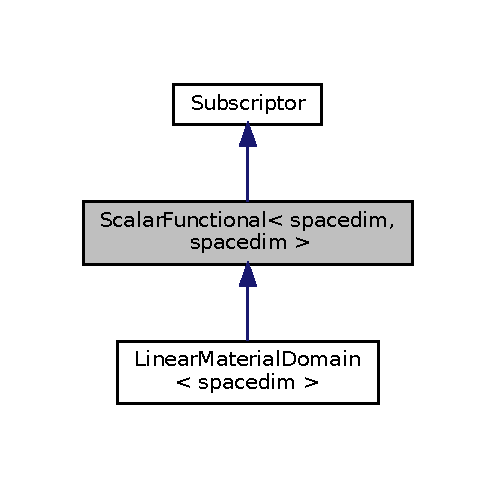
\includegraphics[width=223pt]{class_scalar_functional_3_01spacedim_00_01spacedim_01_4__inherit__graph}
\end{center}
\end{figure}


Collaboration diagram for Scalar\+Functional$<$ spacedim, spacedim $>$\+:
\nopagebreak
\begin{figure}[H]
\begin{center}
\leavevmode
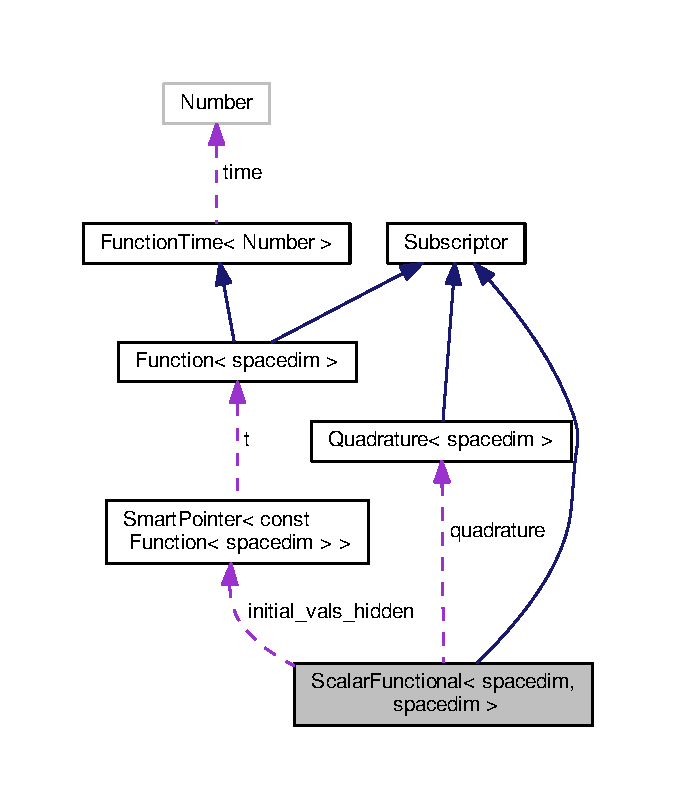
\includegraphics[width=325pt]{class_scalar_functional_3_01spacedim_00_01spacedim_01_4__coll__graph}
\end{center}
\end{figure}
\subsection*{Public Member Functions}
\begin{DoxyCompactItemize}
\item 
\hyperlink{class_scalar_functional_3_01spacedim_00_01spacedim_01_4_a4c4903b402908f26b8c8b433a7cbeb76}{Scalar\+Functional} (const std\+::vector$<$ \hyperlink{class_dependent_field}{Dependent\+Field}$<$ spacedim, spacedim $>$$>$ \hyperlink{class_scalar_functional_3_01spacedim_00_01spacedim_01_4_adfed9b70b743ba245a39c3e63b951f96}{e\+\_\+omega}, const std\+::set$<$ {\bf types\+::material\+\_\+id} $>$ \hyperlink{class_scalar_functional_3_01spacedim_00_01spacedim_01_4_aa192395f822a64f60df43bf9d36c2f3a}{domain\+\_\+of\+\_\+integration}, const {\bf Quadrature}$<$ spacedim $>$ \hyperlink{class_scalar_functional_3_01spacedim_00_01spacedim_01_4_ab83ee3ae077b211137824b006098382e}{quadrature}, const std\+::string \hyperlink{class_scalar_functional_3_01spacedim_00_01spacedim_01_4_a195248af3821548af3000872e9e6d00e}{name}, const unsigned int \hyperlink{class_scalar_functional_3_01spacedim_00_01spacedim_01_4_acee2c3c289e5b2b680996facc2f79e78}{n\+\_\+ref\+\_\+sets}=0, const unsigned int \hyperlink{class_scalar_functional_3_01spacedim_00_01spacedim_01_4_a7df6711471715f907bc9911449c5c825}{n\+\_\+hidden}=0, const {\bf Function}$<$ spacedim $>$ $\ast$const \hyperlink{class_scalar_functional_3_01spacedim_00_01spacedim_01_4_ae3282d5182360e0030e4cc5e02fbe2eb}{initial\+\_\+vals\+\_\+hidden}=nullptr)
\item 
virtual bool \hyperlink{class_scalar_functional_3_01spacedim_00_01spacedim_01_4_a629bfeae4d8ea364fc3f72fea8016ac8}{get\+\_\+h\+\_\+omega} (const {\bf Vector}$<$ double $>$ \&\hyperlink{class_scalar_functional_3_01spacedim_00_01spacedim_01_4_adfed9b70b743ba245a39c3e63b951f96}{e\+\_\+omega}, const std\+::vector$<$ {\bf Vector}$<$ double $>$$>$ \&e\+\_\+omega\+\_\+ref\+\_\+sets, {\bf Vector}$<$ double $>$ \&hidden\+\_\+vars, const {\bf Point}$<$ spacedim $>$ \&x, double \&h\+\_\+omega, {\bf Vector}$<$ double $>$ \&h\+\_\+omega\+\_\+1, {\bf Full\+Matrix}$<$ double $>$ \&h\+\_\+omega\+\_\+2, const std\+::tuple$<$ bool, bool, bool $>$ requested\+\_\+quantities) const =0
\item 
virtual double \hyperlink{class_scalar_functional_3_01spacedim_00_01spacedim_01_4_aba0e5304e9786bf28a25483d467e5d70}{get\+\_\+maximum\+\_\+step} (const {\bf Vector}$<$ double $>$ \&\hyperlink{class_scalar_functional_3_01spacedim_00_01spacedim_01_4_adfed9b70b743ba245a39c3e63b951f96}{e\+\_\+omega}, const std\+::vector$<$ {\bf Vector}$<$ double $>$$>$ \&e\+\_\+omega\+\_\+ref\+\_\+sets, const {\bf Vector}$<$ double $>$ \&delta\+\_\+e\+\_\+omega, const {\bf Vector}$<$ double $>$ \&hidden\+\_\+vars, const {\bf Point}$<$ spacedim $>$ \&x) const 
\item 
void \hyperlink{class_scalar_functional_3_01spacedim_00_01spacedim_01_4_ab7f0d81df4bb8604f0ebc270b64d7f68}{compare\+\_\+derivatives\+\_\+with\+\_\+numerical\+\_\+derivatives} ({\bf Vector}$<$ double $>$ \&\hyperlink{class_scalar_functional_3_01spacedim_00_01spacedim_01_4_adfed9b70b743ba245a39c3e63b951f96}{e\+\_\+omega}, const std\+::vector$<$ {\bf Vector}$<$ double $>$$>$ \&e\+\_\+omega\+\_\+ref\+\_\+sets, {\bf Vector}$<$ double $>$ \&hidden\+\_\+vars, const {\bf Point}$<$ spacedim $>$ \&x, const std\+::string detailed\+\_\+printout\+\_\+file=\char`\"{}\char`\"{}, const double {\bf epsilon}=1e-\/8) const 
\item 
virtual \hyperlink{class_scalar_functional_3_01spacedim_00_01spacedim_01_4_a42b56519b3e4338d248c1e29e29831a6}{$\sim$\+Scalar\+Functional} ()
\end{DoxyCompactItemize}
\subsection*{Public Attributes}
\begin{DoxyCompactItemize}
\item 
const std\+::set$<$ {\bf types\+::material\+\_\+id} $>$ \hyperlink{class_scalar_functional_3_01spacedim_00_01spacedim_01_4_aa192395f822a64f60df43bf9d36c2f3a}{domain\+\_\+of\+\_\+integration}
\item 
const {\bf Smart\+Pointer}$<$ const {\bf Function}$<$ spacedim $>$ $>$ \hyperlink{class_scalar_functional_3_01spacedim_00_01spacedim_01_4_ae3282d5182360e0030e4cc5e02fbe2eb}{initial\+\_\+vals\+\_\+hidden}
\item 
const std\+::vector$<$ \hyperlink{class_dependent_field}{Dependent\+Field}$<$ spacedim, spacedim $>$ $>$ \hyperlink{class_scalar_functional_3_01spacedim_00_01spacedim_01_4_adfed9b70b743ba245a39c3e63b951f96}{e\+\_\+omega}
\item 
const {\bf Quadrature}$<$ spacedim $>$ \hyperlink{class_scalar_functional_3_01spacedim_00_01spacedim_01_4_ab83ee3ae077b211137824b006098382e}{quadrature}
\item 
const unsigned int \hyperlink{class_scalar_functional_3_01spacedim_00_01spacedim_01_4_a7df6711471715f907bc9911449c5c825}{n\+\_\+hidden}
\item 
const std\+::string \hyperlink{class_scalar_functional_3_01spacedim_00_01spacedim_01_4_a195248af3821548af3000872e9e6d00e}{name}
\item 
const unsigned int \hyperlink{class_scalar_functional_3_01spacedim_00_01spacedim_01_4_acee2c3c289e5b2b680996facc2f79e78}{n\+\_\+ref\+\_\+sets}
\end{DoxyCompactItemize}
\subsection*{Additional Inherited Members}


\subsection{Detailed Description}
\subsubsection*{template$<$unsigned int spacedim$>$\\*
class Scalar\+Functional$<$ spacedim, spacedim $>$}

Class defining a domain related scalar functional $H^\Omega_\rho = \int_\Omega h^\Omega_\rho(e^\Omega_\lambda, \boldsymbol{X}) \mathrm{d}V$, where $\rho \in P=\left\{1 \hdots N^\mathrm{H,\Omega}\right\}$.

\char`\"{}\+Hidden\char`\"{} variables involved in the definition of the functions $h^\Omega_\rho$ are allowed for (in order to allow for incorporation of e.\+g. classical plasticity formulations).

The integrand $h^\Omega_\rho$ may, besides the current values of $e^\Omega_\lambda$, also depend on an arbitrary number of sets of \char`\"{}reference values\char`\"{} of $e^\Omega_\lambda$. These reference values can e.\+g. be the values of the $e^\Omega_\lambda$ at previous instants of time. When derivatives of $h^\Omega_\rho$ w.\+r.\+t. the dependent variables are calculated, these reference values are generally regarded as fixed.

In principle, it is often sufficient that the first and second derivatives of $h^\Omega_\rho$ are known, as the values themselves do not factor into the finite element system. However, this depends on the exact problem.

The \hyperlink{class_scalar_functional_3_01spacedim_00_01spacedim_01_4}{Scalar\+Functional$<$spacedim, spacedim$>$} class inherits from {\bf Subscriptor} in order to be able to check that \hyperlink{class_scalar_functional_3_01spacedim_00_01spacedim_01_4}{Scalar\+Functional$<$spacedim, spacedim$>$} objects are only destroyed when they are not needed anymore by other objects.


\begin{DoxyTemplParams}{Template Parameters}
{\em spacedim} & The spatial dimension of the problem \\
\hline
\end{DoxyTemplParams}


\subsection{Constructor \& Destructor Documentation}
\index{Scalar\+Functional$<$ spacedim, spacedim $>$@{Scalar\+Functional$<$ spacedim, spacedim $>$}!Scalar\+Functional@{Scalar\+Functional}}
\index{Scalar\+Functional@{Scalar\+Functional}!Scalar\+Functional$<$ spacedim, spacedim $>$@{Scalar\+Functional$<$ spacedim, spacedim $>$}}
\subsubsection[{\texorpdfstring{Scalar\+Functional(const std\+::vector$<$ Dependent\+Field$<$ spacedim, spacedim $>$$>$ e\+\_\+omega, const std\+::set$<$ types\+::material\+\_\+id $>$ domain\+\_\+of\+\_\+integration, const Quadrature$<$ spacedim $>$ quadrature, const std\+::string name, const unsigned int n\+\_\+ref\+\_\+sets=0, const unsigned int n\+\_\+hidden=0, const Function$<$ spacedim $>$ $\ast$const initial\+\_\+vals\+\_\+hidden=nullptr)}{ScalarFunctional(const std::vector< DependentField< spacedim, spacedim >> e_omega, const std::set< types::material_id > domain_of_integration, const Quadrature< spacedim > quadrature, const std::string name, const unsigned int n_ref_sets=0, const unsigned int n_hidden=0, const Function< spacedim > *const initial_vals_hidden=nullptr)}}]{\setlength{\rightskip}{0pt plus 5cm}template$<$unsigned int spacedim$>$ {\bf Scalar\+Functional}$<$ spacedim, spacedim $>$\+::{\bf Scalar\+Functional} (
\begin{DoxyParamCaption}
\item[{const std\+::vector$<$ {\bf Dependent\+Field}$<$ spacedim, spacedim $>$$>$}]{e\+\_\+omega, }
\item[{const std\+::set$<$ {\bf types\+::material\+\_\+id} $>$}]{domain\+\_\+of\+\_\+integration, }
\item[{const {\bf Quadrature}$<$ spacedim $>$}]{quadrature, }
\item[{const std\+::string}]{name, }
\item[{const unsigned int}]{n\+\_\+ref\+\_\+sets = {\ttfamily 0}, }
\item[{const unsigned int}]{n\+\_\+hidden = {\ttfamily 0}, }
\item[{const {\bf Function}$<$ spacedim $>$ $\ast$const}]{initial\+\_\+vals\+\_\+hidden = {\ttfamily nullptr}}
\end{DoxyParamCaption}
)}\hypertarget{class_scalar_functional_3_01spacedim_00_01spacedim_01_4_a4c4903b402908f26b8c8b433a7cbeb76}{}\label{class_scalar_functional_3_01spacedim_00_01spacedim_01_4_a4c4903b402908f26b8c8b433a7cbeb76}
The constructor of the class


\begin{DoxyParams}[1]{Parameters}
\mbox{\tt in}  & {\em e\+\_\+omega} & \hyperlink{class_scalar_functional_3_01spacedim_00_01spacedim_01_4_adfed9b70b743ba245a39c3e63b951f96}{Scalar\+Functional$<$spacedim, spacedim$>$\+::e\+\_\+omega}\\
\hline
\mbox{\tt in}  & {\em domain\+\_\+of\+\_\+integration} & \hyperlink{class_scalar_functional_3_01spacedim_00_01spacedim_01_4_aa192395f822a64f60df43bf9d36c2f3a}{Scalar\+Functional$<$spacedim, spacedim$>$\+::domain\+\_\+of\+\_\+integration}\\
\hline
\mbox{\tt in}  & {\em quadrature} & \hyperlink{class_scalar_functional_3_01spacedim_00_01spacedim_01_4_ab83ee3ae077b211137824b006098382e}{Scalar\+Functional$<$spacedim, spacedim$>$\+::quadrature}\\
\hline
\mbox{\tt in}  & {\em name} & \hyperlink{class_scalar_functional_3_01spacedim_00_01spacedim_01_4_a195248af3821548af3000872e9e6d00e}{Scalar\+Functional$<$spacedim, spacedim$>$\+::name}\\
\hline
\mbox{\tt in}  & {\em n\+\_\+ref\+\_\+sets} & \hyperlink{class_scalar_functional_3_01spacedim_00_01spacedim_01_4_acee2c3c289e5b2b680996facc2f79e78}{Scalar\+Functional$<$spacedim, spacedim$>$\+::n\+\_\+ref\+\_\+sets}\\
\hline
\mbox{\tt in}  & {\em n\+\_\+hidden} & \hyperlink{class_scalar_functional_3_01spacedim_00_01spacedim_01_4_a7df6711471715f907bc9911449c5c825}{Scalar\+Functional$<$spacedim, spacedim$>$\+::n\+\_\+hidden}\\
\hline
\mbox{\tt in}  & {\em initial\+\_\+vals\+\_\+hidden} & \hyperlink{class_scalar_functional_3_01spacedim_00_01spacedim_01_4_ae3282d5182360e0030e4cc5e02fbe2eb}{Scalar\+Functional$<$spacedim, spacedim$>$\+::initial\+\_\+vals\+\_\+hidden} (if {\ttfamily n\+\_\+hidden$>$0} and this argument is omitted, the initial values will be set to zero) \\
\hline
\end{DoxyParams}
\index{Scalar\+Functional$<$ spacedim, spacedim $>$@{Scalar\+Functional$<$ spacedim, spacedim $>$}!````~Scalar\+Functional@{$\sim$\+Scalar\+Functional}}
\index{````~Scalar\+Functional@{$\sim$\+Scalar\+Functional}!Scalar\+Functional$<$ spacedim, spacedim $>$@{Scalar\+Functional$<$ spacedim, spacedim $>$}}
\subsubsection[{\texorpdfstring{$\sim$\+Scalar\+Functional()}{~ScalarFunctional()}}]{\setlength{\rightskip}{0pt plus 5cm}template$<$unsigned int spacedim$>$ virtual {\bf Scalar\+Functional}$<$ spacedim, spacedim $>$\+::$\sim${\bf Scalar\+Functional} (
\begin{DoxyParamCaption}
{}
\end{DoxyParamCaption}
)\hspace{0.3cm}{\ttfamily [virtual]}}\hypertarget{class_scalar_functional_3_01spacedim_00_01spacedim_01_4_a42b56519b3e4338d248c1e29e29831a6}{}\label{class_scalar_functional_3_01spacedim_00_01spacedim_01_4_a42b56519b3e4338d248c1e29e29831a6}
The destructor of \hyperlink{class_scalar_functional_3_01spacedim_00_01spacedim_01_4}{Scalar\+Functional$<$spacedim, spacedim$>$} essentially checks before destruction that the \hyperlink{class_scalar_functional_3_01spacedim_00_01spacedim_01_4}{Scalar\+Functional$<$spacedim, spacedim$>$} object is not used by other objects. If this is the case, the program will be aborted. 

\subsection{Member Function Documentation}
\index{Scalar\+Functional$<$ spacedim, spacedim $>$@{Scalar\+Functional$<$ spacedim, spacedim $>$}!compare\+\_\+derivatives\+\_\+with\+\_\+numerical\+\_\+derivatives@{compare\+\_\+derivatives\+\_\+with\+\_\+numerical\+\_\+derivatives}}
\index{compare\+\_\+derivatives\+\_\+with\+\_\+numerical\+\_\+derivatives@{compare\+\_\+derivatives\+\_\+with\+\_\+numerical\+\_\+derivatives}!Scalar\+Functional$<$ spacedim, spacedim $>$@{Scalar\+Functional$<$ spacedim, spacedim $>$}}
\subsubsection[{\texorpdfstring{compare\+\_\+derivatives\+\_\+with\+\_\+numerical\+\_\+derivatives(\+Vector$<$ double $>$ \&e\+\_\+omega, const std\+::vector$<$ Vector$<$ double $>$$>$ \&e\+\_\+omega\+\_\+ref\+\_\+sets, Vector$<$ double $>$ \&hidden\+\_\+vars, const Point$<$ spacedim $>$ \&x, const std\+::string detailed\+\_\+printout\+\_\+file="""", const double epsilon=1e-\/8) const }{compare_derivatives_with_numerical_derivatives(Vector< double > &e_omega, const std::vector< Vector< double >> &e_omega_ref_sets, Vector< double > &hidden_vars, const Point< spacedim > &x, const std::string detailed_printout_file="", const double epsilon=1e-8) const }}]{\setlength{\rightskip}{0pt plus 5cm}template$<$unsigned int spacedim$>$ void {\bf Scalar\+Functional}$<$ spacedim, spacedim $>$\+::compare\+\_\+derivatives\+\_\+with\+\_\+numerical\+\_\+derivatives (
\begin{DoxyParamCaption}
\item[{{\bf Vector}$<$ double $>$ \&}]{e\+\_\+omega, }
\item[{const std\+::vector$<$ {\bf Vector}$<$ double $>$$>$ \&}]{e\+\_\+omega\+\_\+ref\+\_\+sets, }
\item[{{\bf Vector}$<$ double $>$ \&}]{hidden\+\_\+vars, }
\item[{const {\bf Point}$<$ spacedim $>$ \&}]{x, }
\item[{const std\+::string}]{detailed\+\_\+printout\+\_\+file = {\ttfamily \char`\"{}\char`\"{}}, }
\item[{const double}]{epsilon = {\ttfamily 1e-\/8}}
\end{DoxyParamCaption}
) const}\hypertarget{class_scalar_functional_3_01spacedim_00_01spacedim_01_4_ab7f0d81df4bb8604f0ebc270b64d7f68}{}\label{class_scalar_functional_3_01spacedim_00_01spacedim_01_4_ab7f0d81df4bb8604f0ebc270b64d7f68}
Function comparing the computed derivatives of the integrand $h^\Omega_\rho$ provided by \hyperlink{class_scalar_functional_3_01spacedim_00_01spacedim_01_4_a629bfeae4d8ea364fc3f72fea8016ac8}{Scalar\+Functional$<$spacedim, spacedim$>$\+::get\+\_\+h\+\_\+omega()} with corresponding numerically computed finite difference based derivatives.

In the case of the first derivative, the numerical derivatives are obtained based on the values for $h^\Omega_\rho$ provided by \hyperlink{class_scalar_functional_3_01spacedim_00_01spacedim_01_4_a629bfeae4d8ea364fc3f72fea8016ac8}{Scalar\+Functional$<$spacedim, spacedim$>$\+::get\+\_\+h\+\_\+omega()}; and in the case of the second derivatives, the numerical derivatives are obtained based on the values for the first derivatives of $h^\Omega_\rho$ provided by \hyperlink{class_scalar_functional_3_01spacedim_00_01spacedim_01_4_a629bfeae4d8ea364fc3f72fea8016ac8}{Scalar\+Functional$<$spacedim, spacedim$>$\+::get\+\_\+h\+\_\+omega()} ). In both cases, a simple forward finite difference approach is used. Generally, the first numerical derivative can only be \char`\"{}correct\char`\"{} if the computation of the value of $h^\Omega_\rho$ is correctly implemented in the function \hyperlink{class_scalar_functional_3_01spacedim_00_01spacedim_01_4_a629bfeae4d8ea364fc3f72fea8016ac8}{Scalar\+Functional$<$spacedim, spacedim$>$\+::get\+\_\+h\+\_\+omega()}; and likewise the second numerical derivative can only be \char`\"{}correct\char`\"{} if the computation of the first derivative of $h^\Omega_\rho$ is correctly implemented in the function \hyperlink{class_scalar_functional_3_01spacedim_00_01spacedim_01_4_a629bfeae4d8ea364fc3f72fea8016ac8}{Scalar\+Functional$<$spacedim, spacedim$>$\+::get\+\_\+h\+\_\+omega()}.

This function is essentially meant for testing of user defined functions \hyperlink{class_scalar_functional_3_01spacedim_00_01spacedim_01_4_a629bfeae4d8ea364fc3f72fea8016ac8}{Scalar\+Functional$<$spacedim, spacedim$>$\+::get\+\_\+h\+\_\+omega()}.


\begin{DoxyParams}[1]{Parameters}
\mbox{\tt in}  & {\em e\+\_\+omega} & Values of $e^\Omega_\lambda$ (the ordering is defined by the ordering of the dependent fields in \hyperlink{class_scalar_functional_3_01spacedim_00_01spacedim_01_4_adfed9b70b743ba245a39c3e63b951f96}{Scalar\+Functional$<$spacedim, spacedim$>$\+::e\+\_\+omega})\\
\hline
\mbox{\tt in}  & {\em e\+\_\+omega\+\_\+ref\+\_\+sets} & Sets of reference values of $e^\Omega_\lambda$ (as required according to \hyperlink{class_scalar_functional_3_01spacedim_00_01spacedim_01_4_acee2c3c289e5b2b680996facc2f79e78}{Scalar\+Functional$<$spacedim, spacedim$>$\+::n\+\_\+ref\+\_\+sets})\\
\hline
\mbox{\tt in,out}  & {\em hidden\+\_\+vars} & Values of \char`\"{}hidden\char`\"{} variables associated with the integrand $h^\Omega_\rho$. This vector has the size \hyperlink{class_scalar_functional_3_01spacedim_00_01spacedim_01_4_a7df6711471715f907bc9911449c5c825}{Scalar\+Functional$<$spacedim, spacedim$>$\+::n\+\_\+hidden}.\\
\hline
\mbox{\tt in}  & {\em x} & Location of material point at which integrand $h^\Omega_\rho$ and derivatives thereof are evaluated\\
\hline
\mbox{\tt in}  & {\em detailed\+\_\+printout\+\_\+file} & A file to which detailed printout is written if requested\\
\hline
\mbox{\tt in}  & {\em epsilon} & Step width for finite difference computation \\
\hline
\end{DoxyParams}
\index{Scalar\+Functional$<$ spacedim, spacedim $>$@{Scalar\+Functional$<$ spacedim, spacedim $>$}!get\+\_\+h\+\_\+omega@{get\+\_\+h\+\_\+omega}}
\index{get\+\_\+h\+\_\+omega@{get\+\_\+h\+\_\+omega}!Scalar\+Functional$<$ spacedim, spacedim $>$@{Scalar\+Functional$<$ spacedim, spacedim $>$}}
\subsubsection[{\texorpdfstring{get\+\_\+h\+\_\+omega(const Vector$<$ double $>$ \&e\+\_\+omega, const std\+::vector$<$ Vector$<$ double $>$$>$ \&e\+\_\+omega\+\_\+ref\+\_\+sets, Vector$<$ double $>$ \&hidden\+\_\+vars, const Point$<$ spacedim $>$ \&x, double \&h\+\_\+omega, Vector$<$ double $>$ \&h\+\_\+omega\+\_\+1, Full\+Matrix$<$ double $>$ \&h\+\_\+omega\+\_\+2, const std\+::tuple$<$ bool, bool, bool $>$ requested\+\_\+quantities) const =0}{get_h_omega(const Vector< double > &e_omega, const std::vector< Vector< double >> &e_omega_ref_sets, Vector< double > &hidden_vars, const Point< spacedim > &x, double &h_omega, Vector< double > &h_omega_1, FullMatrix< double > &h_omega_2, const std::tuple< bool, bool, bool > requested_quantities) const =0}}]{\setlength{\rightskip}{0pt plus 5cm}template$<$unsigned int spacedim$>$ virtual bool {\bf Scalar\+Functional}$<$ spacedim, spacedim $>$\+::get\+\_\+h\+\_\+omega (
\begin{DoxyParamCaption}
\item[{const {\bf Vector}$<$ double $>$ \&}]{e\+\_\+omega, }
\item[{const std\+::vector$<$ {\bf Vector}$<$ double $>$$>$ \&}]{e\+\_\+omega\+\_\+ref\+\_\+sets, }
\item[{{\bf Vector}$<$ double $>$ \&}]{hidden\+\_\+vars, }
\item[{const {\bf Point}$<$ spacedim $>$ \&}]{x, }
\item[{double \&}]{h\+\_\+omega, }
\item[{{\bf Vector}$<$ double $>$ \&}]{h\+\_\+omega\+\_\+1, }
\item[{{\bf Full\+Matrix}$<$ double $>$ \&}]{h\+\_\+omega\+\_\+2, }
\item[{const std\+::tuple$<$ bool, bool, bool $>$}]{requested\+\_\+quantities}
\end{DoxyParamCaption}
) const\hspace{0.3cm}{\ttfamily [pure virtual]}}\hypertarget{class_scalar_functional_3_01spacedim_00_01spacedim_01_4_a629bfeae4d8ea364fc3f72fea8016ac8}{}\label{class_scalar_functional_3_01spacedim_00_01spacedim_01_4_a629bfeae4d8ea364fc3f72fea8016ac8}
Function for evaluation of integrand $h^\Omega_\rho$ and computation of first and second derivatives w.\+r.\+t. the dependent fields $e^\Omega_\lambda$.

This function is pure virtual, and, therefore, it is not possible to instantiate objects of this class. Rather, derived user defined classes must implement this function.


\begin{DoxyParams}[1]{Parameters}
\mbox{\tt in}  & {\em e\+\_\+omega} & Values of $e^\Omega_\lambda$ (the ordering is defined by the ordering of the dependent fields in \hyperlink{class_scalar_functional_3_01spacedim_00_01spacedim_01_4_adfed9b70b743ba245a39c3e63b951f96}{Scalar\+Functional$<$spacedim, spacedim$>$\+::e\+\_\+omega})\\
\hline
\mbox{\tt in}  & {\em e\+\_\+omega\+\_\+ref\+\_\+sets} & Sets of reference values of $e^\Omega_\lambda$ (as required according to \hyperlink{class_scalar_functional_3_01spacedim_00_01spacedim_01_4_acee2c3c289e5b2b680996facc2f79e78}{Scalar\+Functional$<$spacedim, spacedim$>$\+::n\+\_\+ref\+\_\+sets})\\
\hline
\mbox{\tt in,out}  & {\em hidden\+\_\+vars} & Values of \char`\"{}hidden\char`\"{} variables associated with the integrand $h^\Omega_\rho$. This vector has the size \hyperlink{class_scalar_functional_3_01spacedim_00_01spacedim_01_4_a7df6711471715f907bc9911449c5c825}{Scalar\+Functional$<$spacedim, spacedim$>$\+::n\+\_\+hidden}. The inputs are the previously known values of the hidden variables, which may be overwritten by the function (the user can decide during assembly of the finite element system whether the returned updated values of the hidden variables are really used to update the stored values of the hidden variables or whether they are discarded)\\
\hline
\mbox{\tt in}  & {\em x} & Location of material point at which integrand $h^\Omega_\rho$ and derivatives thereof are evaluated\\
\hline
\mbox{\tt out}  & {\em h\+\_\+omega} & Current value of $h^\Omega_\rho$.\\
\hline
\mbox{\tt out}  & {\em h\+\_\+omega\+\_\+1} & First derivatives of $h^\Omega_\rho$ w.\+r.\+t. $e^\Omega_\lambda$ (the ordering is defined by the ordering of the dependent fields in \hyperlink{class_scalar_functional_3_01spacedim_00_01spacedim_01_4_adfed9b70b743ba245a39c3e63b951f96}{Scalar\+Functional$<$spacedim, spacedim$>$\+::e\+\_\+omega}, and {\ttfamily h\+\_\+omega\+\_\+1} will already be initialized to the correct size if it is called by \hyperlink{class_assembly_helper}{Assembly\+Helper} objects)\\
\hline
\mbox{\tt out}  & {\em h\+\_\+omega\+\_\+2} & Second derivatives of $h^\Omega_\rho$ w.\+r.\+t. $e^\Omega_\lambda$ (the ordering is defined by the ordering of the dependent fields in \hyperlink{class_scalar_functional_3_01spacedim_00_01spacedim_01_4_adfed9b70b743ba245a39c3e63b951f96}{Scalar\+Functional$<$spacedim, spacedim$>$\+::e\+\_\+omega}, and {\ttfamily h\+\_\+omega\+\_\+2} will already be initialized to the correct size if it is called by \hyperlink{class_assembly_helper}{Assembly\+Helper} objects). If $h^\Omega_\rho$ exists, this matrix will generally be symmetric. However, in principle the routines do also work for cases where $h^\Omega_\rho$ does not exist and {\ttfamily h\+\_\+omega\+\_\+2} is not symmetric.\\
\hline
\mbox{\tt in}  & {\em requested\+\_\+quantities} & A tuple indicating which quantities are actually to be computed (e.\+g. ({\ttfamily true}, {\ttfamily false}, {\ttfamily true}) indicates that {\ttfamily h\+\_\+omega} and {\ttfamily h\+\_\+omega\+\_\+2} are to be computed)\\
\hline
\end{DoxyParams}
\begin{DoxyReturn}{Returns}
{\ttfamily false} if the evaluation of the integrand $h^\Omega_\rho$ and its derivatives was successful, and {\ttfamily true} if an error prevented the proper calculation of these quantities (e.\+g. because a dependent field, which should be non-\/negative, was actually negative) 
\end{DoxyReturn}


Implemented in \hyperlink{class_linear_material_domain_ac071e6886b4e661442af7a003d5f2b2a}{Linear\+Material\+Domain$<$ spacedim $>$}.

\index{Scalar\+Functional$<$ spacedim, spacedim $>$@{Scalar\+Functional$<$ spacedim, spacedim $>$}!get\+\_\+maximum\+\_\+step@{get\+\_\+maximum\+\_\+step}}
\index{get\+\_\+maximum\+\_\+step@{get\+\_\+maximum\+\_\+step}!Scalar\+Functional$<$ spacedim, spacedim $>$@{Scalar\+Functional$<$ spacedim, spacedim $>$}}
\subsubsection[{\texorpdfstring{get\+\_\+maximum\+\_\+step(const Vector$<$ double $>$ \&e\+\_\+omega, const std\+::vector$<$ Vector$<$ double $>$$>$ \&e\+\_\+omega\+\_\+ref\+\_\+sets, const Vector$<$ double $>$ \&delta\+\_\+e\+\_\+omega, const Vector$<$ double $>$ \&hidden\+\_\+vars, const Point$<$ spacedim $>$ \&x) const }{get_maximum_step(const Vector< double > &e_omega, const std::vector< Vector< double >> &e_omega_ref_sets, const Vector< double > &delta_e_omega, const Vector< double > &hidden_vars, const Point< spacedim > &x) const }}]{\setlength{\rightskip}{0pt plus 5cm}template$<$unsigned int spacedim$>$ virtual double {\bf Scalar\+Functional}$<$ spacedim, spacedim $>$\+::get\+\_\+maximum\+\_\+step (
\begin{DoxyParamCaption}
\item[{const {\bf Vector}$<$ double $>$ \&}]{e\+\_\+omega, }
\item[{const std\+::vector$<$ {\bf Vector}$<$ double $>$$>$ \&}]{e\+\_\+omega\+\_\+ref\+\_\+sets, }
\item[{const {\bf Vector}$<$ double $>$ \&}]{delta\+\_\+e\+\_\+omega, }
\item[{const {\bf Vector}$<$ double $>$ \&}]{hidden\+\_\+vars, }
\item[{const {\bf Point}$<$ spacedim $>$ \&}]{x}
\end{DoxyParamCaption}
) const\hspace{0.3cm}{\ttfamily [virtual]}}\hypertarget{class_scalar_functional_3_01spacedim_00_01spacedim_01_4_aba0e5304e9786bf28a25483d467e5d70}{}\label{class_scalar_functional_3_01spacedim_00_01spacedim_01_4_aba0e5304e9786bf28a25483d467e5d70}
Function for evaluation of the maximum permissible step length


\begin{DoxyParams}[1]{Parameters}
\mbox{\tt in}  & {\em e\+\_\+omega} & Values of $e^\Omega_\lambda$ (the ordering is defined by the ordering of the dependent fields in Scalar\+Functional\+::e\+\_\+omega)\\
\hline
\mbox{\tt in}  & {\em e\+\_\+omega\+\_\+ref\+\_\+sets} & Sets of reference values of $e^\Omega_\lambda$ (as required according to \hyperlink{class_scalar_functional_a7e12423f4b29e9e0aaa0f7f9c2d1c0eb}{Scalar\+Functional\+::n\+\_\+ref\+\_\+sets})\\
\hline
\mbox{\tt in}  & {\em delta\+\_\+e\+\_\+omega} & Values of $\Delta e^\Omega_\lambda$\\
\hline
\mbox{\tt in}  & {\em hidden\+\_\+vars} & Values of \char`\"{}hidden\char`\"{} variables associated with the integrand $h^\Omega_\rho$. This vector has the size \hyperlink{class_scalar_functional_3_01spacedim_00_01spacedim_01_4_a7df6711471715f907bc9911449c5c825}{Scalar\+Functional$<$spacedim, spacedim$>$\+::n\+\_\+hidden}.\\
\hline
\mbox{\tt in}  & {\em x} & Location of material point\\
\hline
\end{DoxyParams}
\begin{DoxyReturn}{Returns}
The maximum $\alpha$ such that $e^\Omega_\lambda + \alpha \Delta e^\Omega_\lambda$ is a permissible state; the standard implementation returns D\+B\+L\+\_\+\+M\+AX 
\end{DoxyReturn}


\subsection{Member Data Documentation}
\index{Scalar\+Functional$<$ spacedim, spacedim $>$@{Scalar\+Functional$<$ spacedim, spacedim $>$}!domain\+\_\+of\+\_\+integration@{domain\+\_\+of\+\_\+integration}}
\index{domain\+\_\+of\+\_\+integration@{domain\+\_\+of\+\_\+integration}!Scalar\+Functional$<$ spacedim, spacedim $>$@{Scalar\+Functional$<$ spacedim, spacedim $>$}}
\subsubsection[{\texorpdfstring{domain\+\_\+of\+\_\+integration}{domain_of_integration}}]{\setlength{\rightskip}{0pt plus 5cm}template$<$unsigned int spacedim$>$ const std\+::set$<${\bf types\+::material\+\_\+id}$>$ {\bf Scalar\+Functional}$<$ spacedim, spacedim $>$\+::domain\+\_\+of\+\_\+integration}\hypertarget{class_scalar_functional_3_01spacedim_00_01spacedim_01_4_aa192395f822a64f60df43bf9d36c2f3a}{}\label{class_scalar_functional_3_01spacedim_00_01spacedim_01_4_aa192395f822a64f60df43bf9d36c2f3a}
Set of {\bf types\+::material\+\_\+id}s determining the domain of integration (i.\+e. those regions of the domain $\Omega$, where the integrand $h^\Omega_\rho$ is non-\/zero). \index{Scalar\+Functional$<$ spacedim, spacedim $>$@{Scalar\+Functional$<$ spacedim, spacedim $>$}!e\+\_\+omega@{e\+\_\+omega}}
\index{e\+\_\+omega@{e\+\_\+omega}!Scalar\+Functional$<$ spacedim, spacedim $>$@{Scalar\+Functional$<$ spacedim, spacedim $>$}}
\subsubsection[{\texorpdfstring{e\+\_\+omega}{e_omega}}]{\setlength{\rightskip}{0pt plus 5cm}template$<$unsigned int spacedim$>$ const std\+::vector$<${\bf Dependent\+Field}$<$spacedim, spacedim$>$ $>$ {\bf Scalar\+Functional}$<$ spacedim, spacedim $>$\+::e\+\_\+omega}\hypertarget{class_scalar_functional_3_01spacedim_00_01spacedim_01_4_adfed9b70b743ba245a39c3e63b951f96}{}\label{class_scalar_functional_3_01spacedim_00_01spacedim_01_4_adfed9b70b743ba245a39c3e63b951f96}
Vector containing the dependent fields $e^\Omega_\lambda$ whereupon the integrand $h^\Omega_\rho$ depends. The ordering in this vector defines the ordering in vectors and matrices related to derivatives of $h^\Omega_\rho$ w.\+r.\+t. the dependent fields $e^\Omega_\lambda$. \index{Scalar\+Functional$<$ spacedim, spacedim $>$@{Scalar\+Functional$<$ spacedim, spacedim $>$}!initial\+\_\+vals\+\_\+hidden@{initial\+\_\+vals\+\_\+hidden}}
\index{initial\+\_\+vals\+\_\+hidden@{initial\+\_\+vals\+\_\+hidden}!Scalar\+Functional$<$ spacedim, spacedim $>$@{Scalar\+Functional$<$ spacedim, spacedim $>$}}
\subsubsection[{\texorpdfstring{initial\+\_\+vals\+\_\+hidden}{initial_vals_hidden}}]{\setlength{\rightskip}{0pt plus 5cm}template$<$unsigned int spacedim$>$ const {\bf Smart\+Pointer}$<$const {\bf Function}$<$spacedim$>$ $>$ {\bf Scalar\+Functional}$<$ spacedim, spacedim $>$\+::initial\+\_\+vals\+\_\+hidden}\hypertarget{class_scalar_functional_3_01spacedim_00_01spacedim_01_4_ae3282d5182360e0030e4cc5e02fbe2eb}{}\label{class_scalar_functional_3_01spacedim_00_01spacedim_01_4_ae3282d5182360e0030e4cc5e02fbe2eb}
A {\bf Function}, which must be supplied by the user for determination of non-\/zero initial values of the hidden variables (applies only if \hyperlink{class_scalar_functional_3_01spacedim_00_01spacedim_01_4_a7df6711471715f907bc9911449c5c825}{Scalar\+Functional$<$spacedim, spacedim$>$\+::n\+\_\+hidden} $>$ 0).

The number of components of \hyperlink{class_scalar_functional_3_01spacedim_00_01spacedim_01_4_ae3282d5182360e0030e4cc5e02fbe2eb}{Scalar\+Functional$<$spacedim, spacedim$>$\+::initial\+\_\+vals\+\_\+hidden} must be equal to \hyperlink{class_scalar_functional_3_01spacedim_00_01spacedim_01_4_a7df6711471715f907bc9911449c5c825}{Scalar\+Functional$<$spacedim, spacedim$>$\+::n\+\_\+hidden}

As a minimum requirement, \hyperlink{class_scalar_functional_3_01spacedim_00_01spacedim_01_4_ae3282d5182360e0030e4cc5e02fbe2eb}{Scalar\+Functional$<$spacedim, spacedim$>$\+::initial\+\_\+vals\+\_\+hidden} must implement the method {\bf Function\+::value()}. \index{Scalar\+Functional$<$ spacedim, spacedim $>$@{Scalar\+Functional$<$ spacedim, spacedim $>$}!n\+\_\+hidden@{n\+\_\+hidden}}
\index{n\+\_\+hidden@{n\+\_\+hidden}!Scalar\+Functional$<$ spacedim, spacedim $>$@{Scalar\+Functional$<$ spacedim, spacedim $>$}}
\subsubsection[{\texorpdfstring{n\+\_\+hidden}{n_hidden}}]{\setlength{\rightskip}{0pt plus 5cm}template$<$unsigned int spacedim$>$ const unsigned int {\bf Scalar\+Functional}$<$ spacedim, spacedim $>$\+::n\+\_\+hidden}\hypertarget{class_scalar_functional_3_01spacedim_00_01spacedim_01_4_a7df6711471715f907bc9911449c5c825}{}\label{class_scalar_functional_3_01spacedim_00_01spacedim_01_4_a7df6711471715f907bc9911449c5c825}
Number of \char`\"{}hidden\char`\"{} variables associated with the integrand $h^\Omega_\rho$ of the scalar functional \index{Scalar\+Functional$<$ spacedim, spacedim $>$@{Scalar\+Functional$<$ spacedim, spacedim $>$}!n\+\_\+ref\+\_\+sets@{n\+\_\+ref\+\_\+sets}}
\index{n\+\_\+ref\+\_\+sets@{n\+\_\+ref\+\_\+sets}!Scalar\+Functional$<$ spacedim, spacedim $>$@{Scalar\+Functional$<$ spacedim, spacedim $>$}}
\subsubsection[{\texorpdfstring{n\+\_\+ref\+\_\+sets}{n_ref_sets}}]{\setlength{\rightskip}{0pt plus 5cm}template$<$unsigned int spacedim$>$ const unsigned int {\bf Scalar\+Functional}$<$ spacedim, spacedim $>$\+::n\+\_\+ref\+\_\+sets}\hypertarget{class_scalar_functional_3_01spacedim_00_01spacedim_01_4_acee2c3c289e5b2b680996facc2f79e78}{}\label{class_scalar_functional_3_01spacedim_00_01spacedim_01_4_acee2c3c289e5b2b680996facc2f79e78}
The number of sets of reference values of the dependent fields $e^\Omega_\lambda$ involved in the definition of the integrand $h^\Omega_\rho$ \index{Scalar\+Functional$<$ spacedim, spacedim $>$@{Scalar\+Functional$<$ spacedim, spacedim $>$}!name@{name}}
\index{name@{name}!Scalar\+Functional$<$ spacedim, spacedim $>$@{Scalar\+Functional$<$ spacedim, spacedim $>$}}
\subsubsection[{\texorpdfstring{name}{name}}]{\setlength{\rightskip}{0pt plus 5cm}template$<$unsigned int spacedim$>$ const std\+::string {\bf Scalar\+Functional}$<$ spacedim, spacedim $>$\+::name}\hypertarget{class_scalar_functional_3_01spacedim_00_01spacedim_01_4_a195248af3821548af3000872e9e6d00e}{}\label{class_scalar_functional_3_01spacedim_00_01spacedim_01_4_a195248af3821548af3000872e9e6d00e}
A name for the scalar functional \index{Scalar\+Functional$<$ spacedim, spacedim $>$@{Scalar\+Functional$<$ spacedim, spacedim $>$}!quadrature@{quadrature}}
\index{quadrature@{quadrature}!Scalar\+Functional$<$ spacedim, spacedim $>$@{Scalar\+Functional$<$ spacedim, spacedim $>$}}
\subsubsection[{\texorpdfstring{quadrature}{quadrature}}]{\setlength{\rightskip}{0pt plus 5cm}template$<$unsigned int spacedim$>$ const {\bf Quadrature}$<$spacedim$>$ {\bf Scalar\+Functional}$<$ spacedim, spacedim $>$\+::quadrature}\hypertarget{class_scalar_functional_3_01spacedim_00_01spacedim_01_4_ab83ee3ae077b211137824b006098382e}{}\label{class_scalar_functional_3_01spacedim_00_01spacedim_01_4_ab83ee3ae077b211137824b006098382e}
{\bf Quadrature} rule when integrating over the domain determined by \hyperlink{class_scalar_functional_3_01spacedim_00_01spacedim_01_4_aa192395f822a64f60df43bf9d36c2f3a}{Scalar\+Functional$<$spacedim, spacedim$>$\+::domain\+\_\+of\+\_\+integration} 

The documentation for this class was generated from the following file\+:\begin{DoxyCompactItemize}
\item 
/home/sst/code/\+Galerkin\+Tools/\+Galerkin\+Tools/include/galerkin\+\_\+tools/\hyperlink{scalar__functional_8h}{scalar\+\_\+functional.\+h}\end{DoxyCompactItemize}

\hypertarget{class_solver_wrapper}{}\doxysection{Solver\+Wrapper$<$ Solution\+Vector\+Type, R\+H\+S\+Vector\+Type, Matrix\+Type, Sparsity\+Pattern\+Type $>$ Class Template Reference}
\label{class_solver_wrapper}\index{SolverWrapper$<$ SolutionVectorType, RHSVectorType, MatrixType, SparsityPatternType $>$@{SolverWrapper$<$ SolutionVectorType, RHSVectorType, MatrixType, SparsityPatternType $>$}}


{\ttfamily \#include $<$solver\+\_\+wrapper.\+h$>$}



Inheritance diagram for Solver\+Wrapper$<$ Solution\+Vector\+Type, R\+H\+S\+Vector\+Type, Matrix\+Type, Sparsity\+Pattern\+Type $>$\+:\nopagebreak
\begin{figure}[H]
\begin{center}
\leavevmode
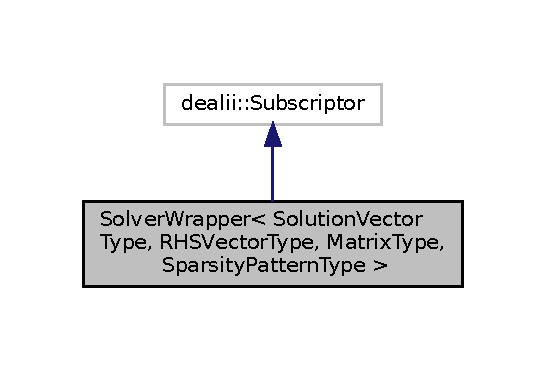
\includegraphics[width=262pt]{class_solver_wrapper__inherit__graph}
\end{center}
\end{figure}


Collaboration diagram for Solver\+Wrapper$<$ Solution\+Vector\+Type, R\+H\+S\+Vector\+Type, Matrix\+Type, Sparsity\+Pattern\+Type $>$\+:\nopagebreak
\begin{figure}[H]
\begin{center}
\leavevmode
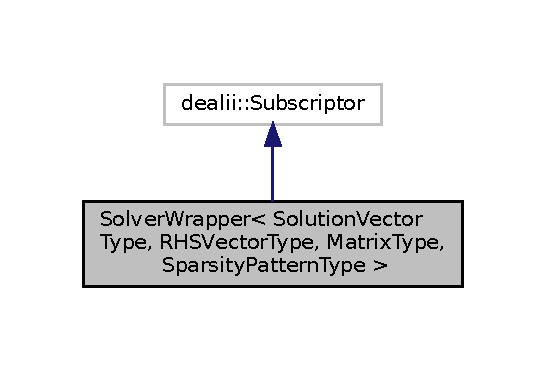
\includegraphics[width=262pt]{class_solver_wrapper__coll__graph}
\end{center}
\end{figure}
\doxysubsection*{Public Member Functions}
\begin{DoxyCompactItemize}
\item 
virtual void \mbox{\hyperlink{class_solver_wrapper_a509594953f388e594bfdde5b927ece35}{solve}} (const \textbf{ Matrix\+Type} \&K\+\_\+stretched, Solution\+Vector\+Type \&solution, const R\+H\+S\+Vector\+Type \&f\+\_\+stretched, const bool \textbf{ symmetric})=0
\item 
virtual \mbox{\hyperlink{class_solver_wrapper_a738e65e298fb0b13327e853fc9683b6d}{$\sim$\+Solver\+Wrapper}} ()
\end{DoxyCompactItemize}


\doxysubsection{Detailed Description}
\subsubsection*{template$<$class Solution\+Vector\+Type, class R\+H\+S\+Vector\+Type, class Matrix\+Type, class Sparsity\+Pattern\+Type$>$\newline
class Solver\+Wrapper$<$ Solution\+Vector\+Type, R\+H\+S\+Vector\+Type, Matrix\+Type, Sparsity\+Pattern\+Type $>$}

This class essentially wraps some functions related to the solver used for the problem and the corresponding data types into a common interface.

The \mbox{\hyperlink{class_solver_wrapper}{Solver\+Wrapper}} class inherits from \textbf{ Subscriptor} in order to be able to check that \mbox{\hyperlink{class_solver_wrapper}{Solver\+Wrapper}} objects are only destroyed when they are not needed anymore by other objects.


\begin{DoxyTemplParams}{Template Parameters}
{\em Solution\+Vector\+Type} & The type used for the solution vector\\
\hline
{\em R\+H\+S\+Vector\+Type} & The type used for the right hand side\\
\hline
{\em Matrix\+Type} & The type used for the system matrix\\
\hline
{\em Sparsity\+Pattern\+Type} & The sparsity pattern used for initialization of the matrix \\
\hline
\end{DoxyTemplParams}


\doxysubsection{Constructor \& Destructor Documentation}
\mbox{\Hypertarget{class_solver_wrapper_a738e65e298fb0b13327e853fc9683b6d}\label{class_solver_wrapper_a738e65e298fb0b13327e853fc9683b6d}} 
\index{SolverWrapper$<$ SolutionVectorType, RHSVectorType, MatrixType, SparsityPatternType $>$@{SolverWrapper$<$ SolutionVectorType, RHSVectorType, MatrixType, SparsityPatternType $>$}!````~SolverWrapper@{$\sim$SolverWrapper}}
\index{````~SolverWrapper@{$\sim$SolverWrapper}!SolverWrapper$<$ SolutionVectorType, RHSVectorType, MatrixType, SparsityPatternType $>$@{SolverWrapper$<$ SolutionVectorType, RHSVectorType, MatrixType, SparsityPatternType $>$}}
\doxysubsubsection{\texorpdfstring{$\sim$SolverWrapper()}{~SolverWrapper()}}
{\footnotesize\ttfamily template$<$class Solution\+Vector\+Type , class R\+H\+S\+Vector\+Type , class Matrix\+Type , class Sparsity\+Pattern\+Type $>$ \\
virtual \mbox{\hyperlink{class_solver_wrapper}{Solver\+Wrapper}}$<$ Solution\+Vector\+Type, R\+H\+S\+Vector\+Type, \textbf{ Matrix\+Type}, Sparsity\+Pattern\+Type $>$\+::$\sim$\mbox{\hyperlink{class_solver_wrapper}{Solver\+Wrapper}} (\begin{DoxyParamCaption}{ }\end{DoxyParamCaption})\hspace{0.3cm}{\ttfamily [virtual]}}

The destructor of \mbox{\hyperlink{class_solver_wrapper}{Solver\+Wrapper}} essentially checks before destruction that the \mbox{\hyperlink{class_solver_wrapper}{Solver\+Wrapper}} object is not used by other objects. If this is the case, the program will be aborted. 

\doxysubsection{Member Function Documentation}
\mbox{\Hypertarget{class_solver_wrapper_a509594953f388e594bfdde5b927ece35}\label{class_solver_wrapper_a509594953f388e594bfdde5b927ece35}} 
\index{SolverWrapper$<$ SolutionVectorType, RHSVectorType, MatrixType, SparsityPatternType $>$@{SolverWrapper$<$ SolutionVectorType, RHSVectorType, MatrixType, SparsityPatternType $>$}!solve@{solve}}
\index{solve@{solve}!SolverWrapper$<$ SolutionVectorType, RHSVectorType, MatrixType, SparsityPatternType $>$@{SolverWrapper$<$ SolutionVectorType, RHSVectorType, MatrixType, SparsityPatternType $>$}}
\doxysubsubsection{\texorpdfstring{solve()}{solve()}}
{\footnotesize\ttfamily template$<$class Solution\+Vector\+Type , class R\+H\+S\+Vector\+Type , class Matrix\+Type , class Sparsity\+Pattern\+Type $>$ \\
virtual void \mbox{\hyperlink{class_solver_wrapper}{Solver\+Wrapper}}$<$ Solution\+Vector\+Type, R\+H\+S\+Vector\+Type, \textbf{ Matrix\+Type}, Sparsity\+Pattern\+Type $>$\+::solve (\begin{DoxyParamCaption}\item[{const \textbf{ Matrix\+Type} \&}]{K\+\_\+stretched,  }\item[{Solution\+Vector\+Type \&}]{solution,  }\item[{const R\+H\+S\+Vector\+Type \&}]{f\+\_\+stretched,  }\item[{const bool}]{symmetric }\end{DoxyParamCaption})\hspace{0.3cm}{\ttfamily [pure virtual]}}

The solve function for the system of linear equations in the stretched form


\begin{DoxyParams}[1]{Parameters}
\mbox{\texttt{ in}}  & {\em K\+\_\+stretched} & The stretched system\+\_\+matrix\\
\hline
\mbox{\texttt{ out}}  & {\em solution} & The stretched solution vector\\
\hline
\mbox{\texttt{ in}}  & {\em f\+\_\+stretched} & The stretched right hand side vector\\
\hline
\mbox{\texttt{ in}}  & {\em symmetric} & A bool indicating whether {\ttfamily system\+\_\+matrix} is symmetric \\
\hline
\end{DoxyParams}


Implemented in \mbox{\hyperlink{class_solver_wrapper_p_e_t_sc_iterative_ade08d6ee2dfb5a6900f99edd8d12fd86}{Solver\+Wrapper\+P\+E\+T\+Sc\+Iterative}}, \mbox{\hyperlink{class_solver_wrapper_p_e_t_sc_a0b4a570ebbfba3dd2fcf116b3f32948b}{Solver\+Wrapper\+P\+E\+T\+Sc}}, and \mbox{\hyperlink{class_solver_wrapper_u_m_f_p_a_c_k_a68f5e2055270d172a4ffdf4a8a4f536e}{Solver\+Wrapper\+U\+M\+F\+P\+A\+CK}}.



The documentation for this class was generated from the following file\+:\begin{DoxyCompactItemize}
\item 
/home/sst/code/\+Galerkin\+Tools/\+Galerkin\+Tools/include/galerkin\+\_\+tools/\mbox{\hyperlink{solver__wrapper_8h}{solver\+\_\+wrapper.\+h}}\end{DoxyCompactItemize}

\hypertarget{class_solver_wrapper_p_e_t_sc}{}\section{Solver\+Wrapper\+P\+E\+T\+Sc Class Reference}
\label{class_solver_wrapper_p_e_t_sc}\index{Solver\+Wrapper\+P\+E\+T\+Sc@{Solver\+Wrapper\+P\+E\+T\+Sc}}


{\ttfamily \#include $<$solver\+\_\+wrapper.\+h$>$}



Inheritance diagram for Solver\+Wrapper\+P\+E\+T\+Sc\+:\nopagebreak
\begin{figure}[H]
\begin{center}
\leavevmode
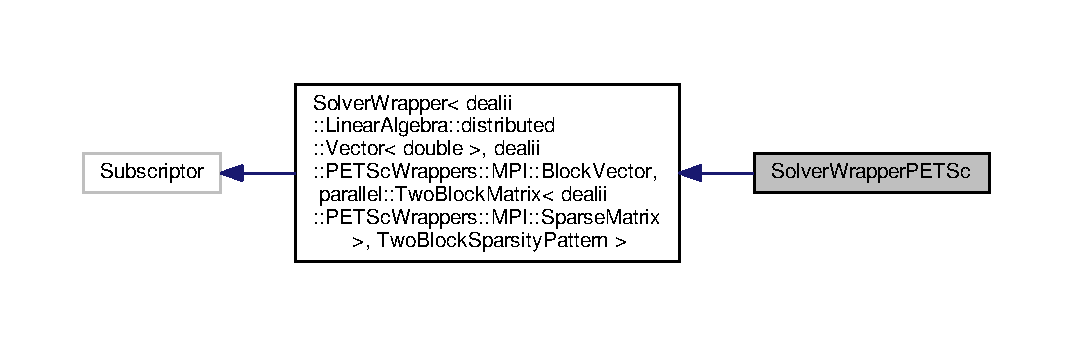
\includegraphics[width=350pt]{class_solver_wrapper_p_e_t_sc__inherit__graph}
\end{center}
\end{figure}


Collaboration diagram for Solver\+Wrapper\+P\+E\+T\+Sc\+:\nopagebreak
\begin{figure}[H]
\begin{center}
\leavevmode
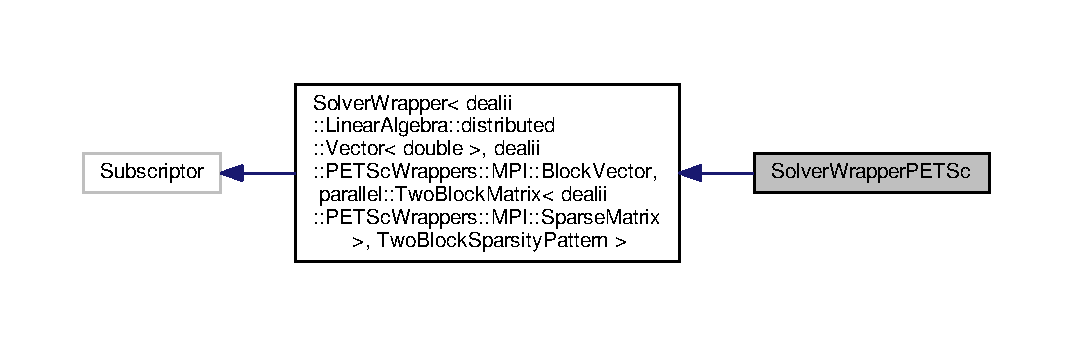
\includegraphics[width=350pt]{class_solver_wrapper_p_e_t_sc__coll__graph}
\end{center}
\end{figure}
\subsection*{Public Member Functions}
\begin{DoxyCompactItemize}
\item 
virtual void \hyperlink{class_solver_wrapper_p_e_t_sc_ac1033bb655ccc7459c4549e5ae4988c5}{solve} (const \hyperlink{classparallel_1_1_two_block_matrix}{parallel\+::\+Two\+Block\+Matrix}$<$ {\bf dealii\+::\+P\+E\+T\+Sc\+Wrappers\+::\+M\+P\+I\+::\+Sparse\+Matrix} $>$ \&K\+\_\+stretched, {\bf dealii\+::\+Linear\+Algebra\+::distributed\+::\+Vector}$<$ double $>$ \&solution, const {\bf dealii\+::\+P\+E\+T\+Sc\+Wrappers\+::\+M\+P\+I\+::\+Block\+Vector} \&f\+\_\+stretched, const bool symmetric=false) const 
\end{DoxyCompactItemize}


\subsection{Detailed Description}
A \hyperlink{class_solver_wrapper}{Solver\+Wrapper} for the P\+E\+T\+Sc M\+U\+M\+PS solver, which works for parallel computations. 

\subsection{Member Function Documentation}
\index{Solver\+Wrapper\+P\+E\+T\+Sc@{Solver\+Wrapper\+P\+E\+T\+Sc}!solve@{solve}}
\index{solve@{solve}!Solver\+Wrapper\+P\+E\+T\+Sc@{Solver\+Wrapper\+P\+E\+T\+Sc}}
\subsubsection[{\texorpdfstring{solve(const parallel\+::\+Two\+Block\+Matrix$<$ dealii\+::\+P\+E\+T\+Sc\+Wrappers\+::\+M\+P\+I\+::\+Sparse\+Matrix $>$ \&\+K\+\_\+stretched, dealii\+::\+Linear\+Algebra\+::distributed\+::\+Vector$<$ double $>$ \&solution, const dealii\+::\+P\+E\+T\+Sc\+Wrappers\+::\+M\+P\+I\+::\+Block\+Vector \&f\+\_\+stretched, const bool symmetric=false) const }{solve(const parallel::TwoBlockMatrix< dealii::PETScWrappers::MPI::SparseMatrix > &K_stretched, dealii::LinearAlgebra::distributed::Vector< double > &solution, const dealii::PETScWrappers::MPI::BlockVector &f_stretched, const bool symmetric=false) const }}]{\setlength{\rightskip}{0pt plus 5cm}virtual void Solver\+Wrapper\+P\+E\+T\+Sc\+::solve (
\begin{DoxyParamCaption}
\item[{const {\bf parallel\+::\+Two\+Block\+Matrix}$<$ {\bf dealii\+::\+P\+E\+T\+Sc\+Wrappers\+::\+M\+P\+I\+::\+Sparse\+Matrix} $>$ \&}]{K\+\_\+stretched, }
\item[{{\bf dealii\+::\+Linear\+Algebra\+::distributed\+::\+Vector}$<$ double $>$ \&}]{solution, }
\item[{const {\bf dealii\+::\+P\+E\+T\+Sc\+Wrappers\+::\+M\+P\+I\+::\+Block\+Vector} \&}]{f\+\_\+stretched, }
\item[{const bool}]{symmetric = {\ttfamily false}}
\end{DoxyParamCaption}
) const\hspace{0.3cm}{\ttfamily [virtual]}}\hypertarget{class_solver_wrapper_p_e_t_sc_ac1033bb655ccc7459c4549e5ae4988c5}{}\label{class_solver_wrapper_p_e_t_sc_ac1033bb655ccc7459c4549e5ae4988c5}




The solve function for the system of linear equations in the stretched form


\begin{DoxyParams}[1]{Parameters}
\mbox{\tt in}  & {\em K\+\_\+stretched} & The stretched system\+\_\+matrix\\
\hline
\mbox{\tt out}  & {\em solution} & The stretched solution vector\\
\hline
\mbox{\tt in}  & {\em f\+\_\+stretched} & The stretched right hand side vector\\
\hline
\mbox{\tt in}  & {\em symmetric} & A bool indicating whether {\ttfamily system\+\_\+matrix} is symmetric \\
\hline
\end{DoxyParams}


Implements \hyperlink{class_solver_wrapper_a75a599630086e2edee14eb43ae071733}{Solver\+Wrapper$<$ dealii\+::\+Linear\+Algebra\+::distributed\+::\+Vector$<$ double $>$, dealii\+::\+P\+E\+T\+Sc\+Wrappers\+::\+M\+P\+I\+::\+Block\+Vector, parallel\+::\+Two\+Block\+Matrix$<$ dealii\+::\+P\+E\+T\+Sc\+Wrappers\+::\+M\+P\+I\+::\+Sparse\+Matrix $>$, Two\+Block\+Sparsity\+Pattern $>$}.



The documentation for this class was generated from the following file\+:\begin{DoxyCompactItemize}
\item 
/home/sst/code/\+Galerkin\+Tools/\+Galerkin\+Tools/include/galerkin\+\_\+tools/\hyperlink{solver__wrapper_8h}{solver\+\_\+wrapper.\+h}\end{DoxyCompactItemize}

\hypertarget{class_solver_wrapper_p_e_t_sc_iterative}{}\section{Solver\+Wrapper\+P\+E\+T\+Sc\+Iterative Class Reference}
\label{class_solver_wrapper_p_e_t_sc_iterative}\index{Solver\+Wrapper\+P\+E\+T\+Sc\+Iterative@{Solver\+Wrapper\+P\+E\+T\+Sc\+Iterative}}


{\ttfamily \#include $<$solver\+\_\+wrapper.\+h$>$}



Inheritance diagram for Solver\+Wrapper\+P\+E\+T\+Sc\+Iterative\+:
\nopagebreak
\begin{figure}[H]
\begin{center}
\leavevmode
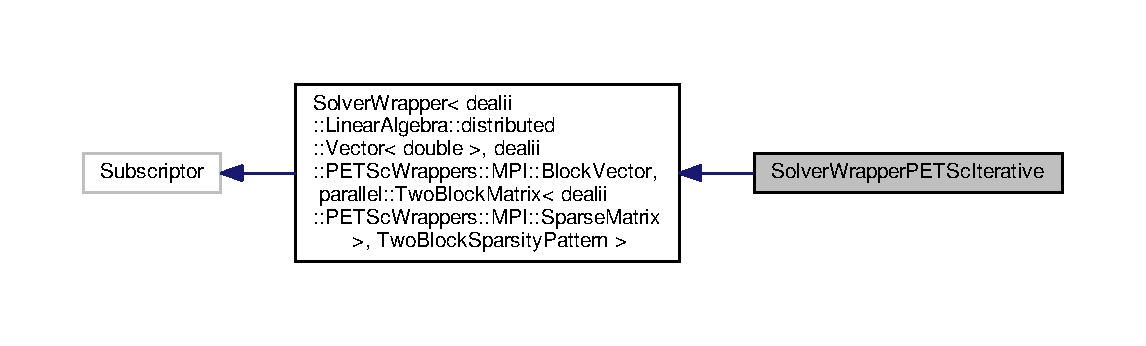
\includegraphics[width=350pt]{class_solver_wrapper_p_e_t_sc_iterative__inherit__graph}
\end{center}
\end{figure}


Collaboration diagram for Solver\+Wrapper\+P\+E\+T\+Sc\+Iterative\+:
\nopagebreak
\begin{figure}[H]
\begin{center}
\leavevmode
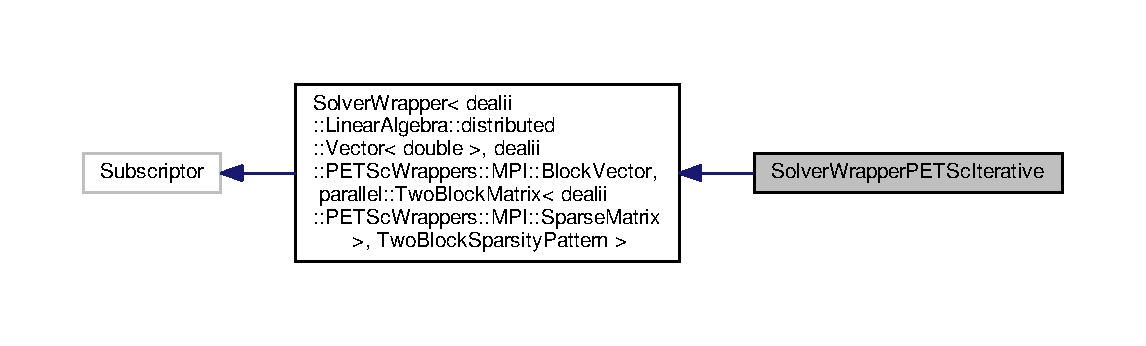
\includegraphics[width=350pt]{class_solver_wrapper_p_e_t_sc_iterative__coll__graph}
\end{center}
\end{figure}
\subsection*{Public Member Functions}
\begin{DoxyCompactItemize}
\item 
virtual void \hyperlink{class_solver_wrapper_p_e_t_sc_iterative_a22441581003123bc0ecefde1cf0f121a}{solve} (const \hyperlink{classparallel_1_1_two_block_matrix}{parallel\+::\+Two\+Block\+Matrix}$<$ {\bf dealii\+::\+P\+E\+T\+Sc\+Wrappers\+::\+M\+P\+I\+::\+Sparse\+Matrix} $>$ \&K\+\_\+stretched, {\bf dealii\+::\+Linear\+Algebra\+::distributed\+::\+Vector}$<$ double $>$ \&solution, const {\bf dealii\+::\+P\+E\+T\+Sc\+Wrappers\+::\+M\+P\+I\+::\+Block\+Vector} \&f\+\_\+stretched, const bool symmetric=false) const 
\end{DoxyCompactItemize}


\subsection{Detailed Description}
A \hyperlink{class_solver_wrapper}{Solver\+Wrapper} for the P\+E\+T\+Sc M\+U\+M\+PS solver, which works for parallel computations. 

\subsection{Member Function Documentation}
\index{Solver\+Wrapper\+P\+E\+T\+Sc\+Iterative@{Solver\+Wrapper\+P\+E\+T\+Sc\+Iterative}!solve@{solve}}
\index{solve@{solve}!Solver\+Wrapper\+P\+E\+T\+Sc\+Iterative@{Solver\+Wrapper\+P\+E\+T\+Sc\+Iterative}}
\subsubsection[{\texorpdfstring{solve(const parallel\+::\+Two\+Block\+Matrix$<$ dealii\+::\+P\+E\+T\+Sc\+Wrappers\+::\+M\+P\+I\+::\+Sparse\+Matrix $>$ \&\+K\+\_\+stretched, dealii\+::\+Linear\+Algebra\+::distributed\+::\+Vector$<$ double $>$ \&solution, const dealii\+::\+P\+E\+T\+Sc\+Wrappers\+::\+M\+P\+I\+::\+Block\+Vector \&f\+\_\+stretched, const bool symmetric=false) const }{solve(const parallel::TwoBlockMatrix< dealii::PETScWrappers::MPI::SparseMatrix > &K_stretched, dealii::LinearAlgebra::distributed::Vector< double > &solution, const dealii::PETScWrappers::MPI::BlockVector &f_stretched, const bool symmetric=false) const }}]{\setlength{\rightskip}{0pt plus 5cm}virtual void Solver\+Wrapper\+P\+E\+T\+Sc\+Iterative\+::solve (
\begin{DoxyParamCaption}
\item[{const {\bf parallel\+::\+Two\+Block\+Matrix}$<$ {\bf dealii\+::\+P\+E\+T\+Sc\+Wrappers\+::\+M\+P\+I\+::\+Sparse\+Matrix} $>$ \&}]{K\+\_\+stretched, }
\item[{{\bf dealii\+::\+Linear\+Algebra\+::distributed\+::\+Vector}$<$ double $>$ \&}]{solution, }
\item[{const {\bf dealii\+::\+P\+E\+T\+Sc\+Wrappers\+::\+M\+P\+I\+::\+Block\+Vector} \&}]{f\+\_\+stretched, }
\item[{const bool}]{symmetric = {\ttfamily false}}
\end{DoxyParamCaption}
) const\hspace{0.3cm}{\ttfamily [virtual]}}\hypertarget{class_solver_wrapper_p_e_t_sc_iterative_a22441581003123bc0ecefde1cf0f121a}{}\label{class_solver_wrapper_p_e_t_sc_iterative_a22441581003123bc0ecefde1cf0f121a}




The solve function for the system of linear equations in the stretched form


\begin{DoxyParams}[1]{Parameters}
\mbox{\tt in}  & {\em K\+\_\+stretched} & The stretched system\+\_\+matrix\\
\hline
\mbox{\tt out}  & {\em solution} & The stretched solution vector\\
\hline
\mbox{\tt in}  & {\em f\+\_\+stretched} & The stretched right hand side vector\\
\hline
\mbox{\tt in}  & {\em symmetric} & A bool indicating whether {\ttfamily system\+\_\+matrix} is symmetric \\
\hline
\end{DoxyParams}


Implements \hyperlink{class_solver_wrapper_a75a599630086e2edee14eb43ae071733}{Solver\+Wrapper$<$ dealii\+::\+Linear\+Algebra\+::distributed\+::\+Vector$<$ double $>$, dealii\+::\+P\+E\+T\+Sc\+Wrappers\+::\+M\+P\+I\+::\+Block\+Vector, parallel\+::\+Two\+Block\+Matrix$<$ dealii\+::\+P\+E\+T\+Sc\+Wrappers\+::\+M\+P\+I\+::\+Sparse\+Matrix $>$, Two\+Block\+Sparsity\+Pattern $>$}.



The documentation for this class was generated from the following file\+:\begin{DoxyCompactItemize}
\item 
/home/sst/code/\+Galerkin\+Tools/\+Galerkin\+Tools/include/galerkin\+\_\+tools/\hyperlink{solver__wrapper_8h}{solver\+\_\+wrapper.\+h}\end{DoxyCompactItemize}

\hypertarget{class_solver_wrapper_u_m_f_p_a_c_k}{}\section{Solver\+Wrapper\+U\+M\+F\+P\+A\+CK Class Reference}
\label{class_solver_wrapper_u_m_f_p_a_c_k}\index{Solver\+Wrapper\+U\+M\+F\+P\+A\+CK@{Solver\+Wrapper\+U\+M\+F\+P\+A\+CK}}


{\ttfamily \#include $<$solver\+\_\+wrapper.\+h$>$}



Inheritance diagram for Solver\+Wrapper\+U\+M\+F\+P\+A\+CK\+:\nopagebreak
\begin{figure}[H]
\begin{center}
\leavevmode
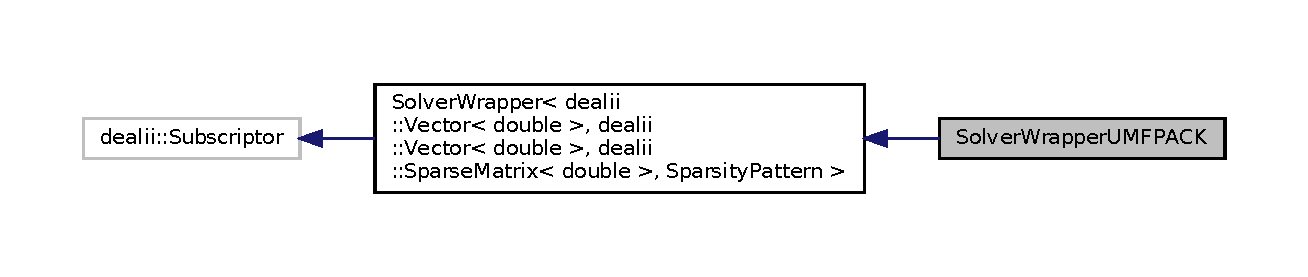
\includegraphics[width=350pt]{class_solver_wrapper_u_m_f_p_a_c_k__inherit__graph}
\end{center}
\end{figure}


Collaboration diagram for Solver\+Wrapper\+U\+M\+F\+P\+A\+CK\+:\nopagebreak
\begin{figure}[H]
\begin{center}
\leavevmode
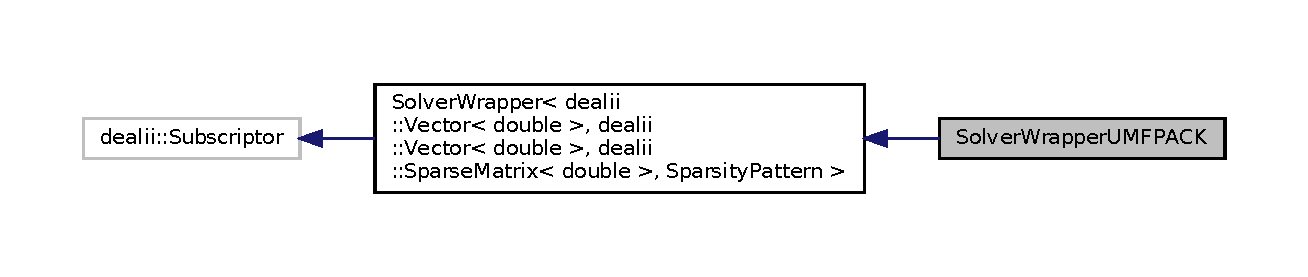
\includegraphics[width=350pt]{class_solver_wrapper_u_m_f_p_a_c_k__coll__graph}
\end{center}
\end{figure}
\subsection*{Public Member Functions}
\begin{DoxyCompactItemize}
\item 
virtual void \hyperlink{class_solver_wrapper_u_m_f_p_a_c_k_a80ed8c6186251e670960945e9ebc0c5b}{solve} (const {\bf dealii\+::\+Sparse\+Matrix}$<$ double $>$ \&K\+\_\+stretched, {\bf dealii\+::\+Vector}$<$ double $>$ \&solution, const {\bf dealii\+::\+Vector}$<$ double $>$ \&f\+\_\+stretched, const bool symmetric=false) const 
\end{DoxyCompactItemize}


\subsection{Detailed Description}
A \hyperlink{class_solver_wrapper}{Solver\+Wrapper} for the direct solver from U\+M\+F\+P\+A\+CK 

\subsection{Member Function Documentation}
\index{Solver\+Wrapper\+U\+M\+F\+P\+A\+CK@{Solver\+Wrapper\+U\+M\+F\+P\+A\+CK}!solve@{solve}}
\index{solve@{solve}!Solver\+Wrapper\+U\+M\+F\+P\+A\+CK@{Solver\+Wrapper\+U\+M\+F\+P\+A\+CK}}
\subsubsection[{\texorpdfstring{solve(const dealii\+::\+Sparse\+Matrix$<$ double $>$ \&\+K\+\_\+stretched, dealii\+::\+Vector$<$ double $>$ \&solution, const dealii\+::\+Vector$<$ double $>$ \&f\+\_\+stretched, const bool symmetric=false) const }{solve(const dealii::SparseMatrix< double > &K_stretched, dealii::Vector< double > &solution, const dealii::Vector< double > &f_stretched, const bool symmetric=false) const }}]{\setlength{\rightskip}{0pt plus 5cm}virtual void Solver\+Wrapper\+U\+M\+F\+P\+A\+C\+K\+::solve (
\begin{DoxyParamCaption}
\item[{const {\bf dealii\+::\+Sparse\+Matrix}$<$ double $>$ \&}]{K\+\_\+stretched, }
\item[{{\bf dealii\+::\+Vector}$<$ double $>$ \&}]{solution, }
\item[{const {\bf dealii\+::\+Vector}$<$ double $>$ \&}]{f\+\_\+stretched, }
\item[{const bool}]{symmetric = {\ttfamily false}}
\end{DoxyParamCaption}
) const\hspace{0.3cm}{\ttfamily [virtual]}}\hypertarget{class_solver_wrapper_u_m_f_p_a_c_k_a80ed8c6186251e670960945e9ebc0c5b}{}\label{class_solver_wrapper_u_m_f_p_a_c_k_a80ed8c6186251e670960945e9ebc0c5b}




The solve function for the system of linear equations in the stretched form


\begin{DoxyParams}[1]{Parameters}
\mbox{\tt in}  & {\em K\+\_\+stretched} & The stretched system\+\_\+matrix\\
\hline
\mbox{\tt out}  & {\em solution} & The stretched solution vector\\
\hline
\mbox{\tt in}  & {\em f\+\_\+stretched} & The stretched right hand side vector\\
\hline
\mbox{\tt in}  & {\em symmetric} & A bool indicating whether {\ttfamily system\+\_\+matrix} is symmetric \\
\hline
\end{DoxyParams}


Implements \hyperlink{class_solver_wrapper_a75a599630086e2edee14eb43ae071733}{Solver\+Wrapper$<$ dealii\+::\+Vector$<$ double $>$, dealii\+::\+Vector$<$ double $>$, dealii\+::\+Sparse\+Matrix$<$ double $>$, Sparsity\+Pattern $>$}.



The documentation for this class was generated from the following file\+:\begin{DoxyCompactItemize}
\item 
/home/sst/code/\+Galerkin\+Tools/\+Galerkin\+Tools/include/galerkin\+\_\+tools/\hyperlink{solver__wrapper_8h}{solver\+\_\+wrapper.\+h}\end{DoxyCompactItemize}

\hypertarget{class_total_potential}{}\doxysection{Total\+Potential$<$ spacedim $>$ Class Template Reference}
\label{class_total_potential}\index{TotalPotential$<$ spacedim $>$@{TotalPotential$<$ spacedim $>$}}


{\ttfamily \#include $<$total\+\_\+potential.\+h$>$}

\doxysubsection*{Public Member Functions}
\begin{DoxyCompactItemize}
\item 
void \mbox{\hyperlink{class_total_potential_ace8b22eef7789f5c7eb78606ba1f110c}{add\+\_\+total\+\_\+potential\+\_\+contribution}} (const \mbox{\hyperlink{class_total_potential_contribution}{Total\+Potential\+Contribution}}$<$ spacedim $>$ \&total\+\_\+potential\+\_\+contribution)
\end{DoxyCompactItemize}
\doxysubsection*{Private Attributes}
\begin{DoxyCompactItemize}
\item 
std\+::vector$<$ \textbf{ Smart\+Pointer}$<$ const \mbox{\hyperlink{class_total_potential_contribution}{Total\+Potential\+Contribution}}$<$ spacedim $>$ $>$ $>$ \mbox{\hyperlink{class_total_potential_a5a14ce0e2fabf8116566aa67fb11db35}{total\+\_\+potential\+\_\+contributions}}
\item 
unsigned int \mbox{\hyperlink{class_total_potential_a800f9366116679fd0f7d3173a3bfc539}{max\+\_\+dependent\+\_\+vars}} = 0
\end{DoxyCompactItemize}
\doxysubsection*{Friends}
\begin{DoxyCompactItemize}
\item 
{\footnotesize template$<$unsigned int $>$ }\\class \mbox{\hyperlink{class_total_potential_af4019c2e39cc934d646aaa35c3c52773}{Assembly\+Helper}}
\end{DoxyCompactItemize}


\doxysubsection{Detailed Description}
\subsubsection*{template$<$unsigned int spacedim$>$\newline
class Total\+Potential$<$ spacedim $>$}

Class collecting all \mbox{\hyperlink{class_total_potential_contribution}{Total\+Potential\+Contribution}} objects $\Pi_i$ in the total potential $\Pi$ according to \begin{equation*} \Pi = \Pi(H^\Omega_\rho, H^\Sigma_\tau, C_\iota) = \sum_i \Pi_i(H^\Omega_\rho, H^\Sigma_\tau, C_\iota). \end{equation*}


\begin{DoxyTemplParams}{Template Parameters}
{\em spacedim} & Spatial dimension \\
\hline
\end{DoxyTemplParams}


\doxysubsection{Member Function Documentation}
\mbox{\Hypertarget{class_total_potential_ace8b22eef7789f5c7eb78606ba1f110c}\label{class_total_potential_ace8b22eef7789f5c7eb78606ba1f110c}} 
\index{TotalPotential$<$ spacedim $>$@{TotalPotential$<$ spacedim $>$}!add\_total\_potential\_contribution@{add\_total\_potential\_contribution}}
\index{add\_total\_potential\_contribution@{add\_total\_potential\_contribution}!TotalPotential$<$ spacedim $>$@{TotalPotential$<$ spacedim $>$}}
\doxysubsubsection{\texorpdfstring{add\_total\_potential\_contribution()}{add\_total\_potential\_contribution()}}
{\footnotesize\ttfamily template$<$unsigned int spacedim$>$ \\
void \mbox{\hyperlink{class_total_potential}{Total\+Potential}}$<$ spacedim $>$\+::add\+\_\+total\+\_\+potential\+\_\+contribution (\begin{DoxyParamCaption}\item[{const \mbox{\hyperlink{class_total_potential_contribution}{Total\+Potential\+Contribution}}$<$ spacedim $>$ \&}]{total\+\_\+potential\+\_\+contribution }\end{DoxyParamCaption})}

Add a contribution $\Pi_i$ to the total potential (i.\+e. to \mbox{\hyperlink{class_total_potential_a5a14ce0e2fabf8116566aa67fb11db35}{Total\+Potential\+::total\+\_\+potential\+\_\+contributions}})


\begin{DoxyParams}[1]{Parameters}
\mbox{\texttt{ in}}  & {\em total\+\_\+potential\+\_\+contribution} & A contribution $\Pi_i$ \\
\hline
\end{DoxyParams}


\doxysubsection{Friends And Related Function Documentation}
\mbox{\Hypertarget{class_total_potential_af4019c2e39cc934d646aaa35c3c52773}\label{class_total_potential_af4019c2e39cc934d646aaa35c3c52773}} 
\index{TotalPotential$<$ spacedim $>$@{TotalPotential$<$ spacedim $>$}!AssemblyHelper@{AssemblyHelper}}
\index{AssemblyHelper@{AssemblyHelper}!TotalPotential$<$ spacedim $>$@{TotalPotential$<$ spacedim $>$}}
\doxysubsubsection{\texorpdfstring{AssemblyHelper}{AssemblyHelper}}
{\footnotesize\ttfamily template$<$unsigned int spacedim$>$ \\
template$<$unsigned int $>$ \\
friend class \mbox{\hyperlink{class_assembly_helper}{Assembly\+Helper}}\hspace{0.3cm}{\ttfamily [friend]}}

\mbox{\hyperlink{class_assembly_helper}{Assembly\+Helper}} is a friend of \mbox{\hyperlink{class_total_potential}{Total\+Potential}} to get direct access to \mbox{\hyperlink{class_total_potential_a5a14ce0e2fabf8116566aa67fb11db35}{Total\+Potential\+::total\+\_\+potential\+\_\+contributions}} and \mbox{\hyperlink{class_total_potential_a800f9366116679fd0f7d3173a3bfc539}{Total\+Potential\+::max\+\_\+dependent\+\_\+vars}} 

\doxysubsection{Member Data Documentation}
\mbox{\Hypertarget{class_total_potential_a800f9366116679fd0f7d3173a3bfc539}\label{class_total_potential_a800f9366116679fd0f7d3173a3bfc539}} 
\index{TotalPotential$<$ spacedim $>$@{TotalPotential$<$ spacedim $>$}!max\_dependent\_vars@{max\_dependent\_vars}}
\index{max\_dependent\_vars@{max\_dependent\_vars}!TotalPotential$<$ spacedim $>$@{TotalPotential$<$ spacedim $>$}}
\doxysubsubsection{\texorpdfstring{max\_dependent\_vars}{max\_dependent\_vars}}
{\footnotesize\ttfamily template$<$unsigned int spacedim$>$ \\
unsigned int \mbox{\hyperlink{class_total_potential}{Total\+Potential}}$<$ spacedim $>$\+::max\+\_\+dependent\+\_\+vars = 0\hspace{0.3cm}{\ttfamily [private]}}

Maximum number of dependent variables in a \mbox{\hyperlink{class_scalar_functional}{Scalar\+Functional}} (or \mbox{\hyperlink{class_scalar_functional_3_01spacedim_00_01spacedim_01_4}{Scalar\+Functional$<$spacedim, spacedim$>$}}, respectively). This information is used internally to reserve an appropriate amount of memory for certain vectors and matrices. \mbox{\Hypertarget{class_total_potential_a5a14ce0e2fabf8116566aa67fb11db35}\label{class_total_potential_a5a14ce0e2fabf8116566aa67fb11db35}} 
\index{TotalPotential$<$ spacedim $>$@{TotalPotential$<$ spacedim $>$}!total\_potential\_contributions@{total\_potential\_contributions}}
\index{total\_potential\_contributions@{total\_potential\_contributions}!TotalPotential$<$ spacedim $>$@{TotalPotential$<$ spacedim $>$}}
\doxysubsubsection{\texorpdfstring{total\_potential\_contributions}{total\_potential\_contributions}}
{\footnotesize\ttfamily template$<$unsigned int spacedim$>$ \\
std\+::vector$<$ \textbf{ Smart\+Pointer}$<$const \mbox{\hyperlink{class_total_potential_contribution}{Total\+Potential\+Contribution}}$<$spacedim$>$ $>$ $>$ \mbox{\hyperlink{class_total_potential}{Total\+Potential}}$<$ spacedim $>$\+::total\+\_\+potential\+\_\+contributions\hspace{0.3cm}{\ttfamily [private]}}

Collection of the \mbox{\hyperlink{class_total_potential_contribution}{Total\+Potential\+Contribution}} objects corresponding to the $\Pi_i$ 

The documentation for this class was generated from the following file\+:\begin{DoxyCompactItemize}
\item 
/home/sst/code/\+Galerkin\+Tools/\+Galerkin\+Tools/include/galerkin\+\_\+tools/\mbox{\hyperlink{total__potential_8h}{total\+\_\+potential.\+h}}\end{DoxyCompactItemize}

\hypertarget{class_total_potential_contribution}{}\section{Total\+Potential\+Contribution$<$ spacedim $>$ Class Template Reference}
\label{class_total_potential_contribution}\index{Total\+Potential\+Contribution$<$ spacedim $>$@{Total\+Potential\+Contribution$<$ spacedim $>$}}


{\ttfamily \#include $<$total\+\_\+potential\+\_\+contribution.\+h$>$}



Inheritance diagram for Total\+Potential\+Contribution$<$ spacedim $>$\+:\nopagebreak
\begin{figure}[H]
\begin{center}
\leavevmode
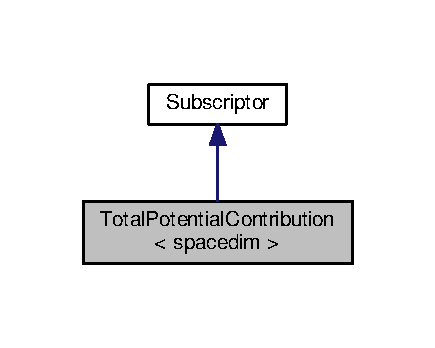
\includegraphics[width=209pt]{class_total_potential_contribution__inherit__graph}
\end{center}
\end{figure}


Collaboration diagram for Total\+Potential\+Contribution$<$ spacedim $>$\+:\nopagebreak
\begin{figure}[H]
\begin{center}
\leavevmode
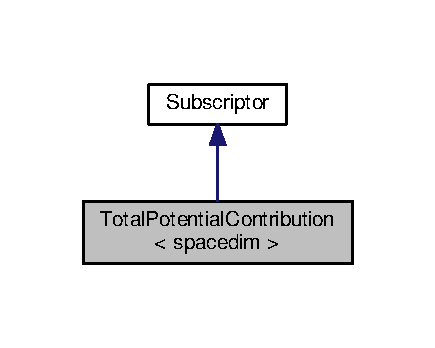
\includegraphics[width=209pt]{class_total_potential_contribution__coll__graph}
\end{center}
\end{figure}
\subsection*{Public Member Functions}
\begin{DoxyCompactItemize}
\item 
virtual bool \hyperlink{class_total_potential_contribution_a0d281fceeb90ece5c4d2655df5eb9948}{get\+\_\+potential\+\_\+contribution} (const {\bf Vector}$<$ double $>$ \&H\+\_\+omega\+\_\+\+H\+\_\+sigma\+\_\+C, const std\+::vector$<$ {\bf Vector}$<$ double $>$$>$ \&C\+\_\+ref\+\_\+sets, double \&Pi, {\bf Vector}$<$ double $>$ \&Pi\+\_\+1, {\bf Full\+Matrix}$<$ double $>$ \&Pi\+\_\+2, const std\+::tuple$<$ bool, bool, bool $>$ \&requested\+\_\+quantities) const 
\item 
\hyperlink{class_total_potential_contribution_a1932d6d7c269344542fc8e9221de4448}{Total\+Potential\+Contribution} (const std\+::vector$<$ const \hyperlink{class_scalar_functional}{Scalar\+Functional}$<$ spacedim, spacedim $>$ $\ast$ $>$ \&\hyperlink{class_total_potential_contribution_a15191539345978a3d0c7293bd7ecaa91}{H\+\_\+omega}, const std\+::vector$<$ const \hyperlink{class_scalar_functional}{Scalar\+Functional}$<$ spacedim-\/1, spacedim $>$ $\ast$ $>$ \&\hyperlink{class_total_potential_contribution_aac404e3a8493d9170541e34bd96673d3}{H\+\_\+sigma}, const std\+::vector$<$ const \hyperlink{class_independent_field}{Independent\+Field}$<$ 0, spacedim $>$ $\ast$ $>$ \&\hyperlink{class_total_potential_contribution_adea8f8f88243adec43df300e8c8d4593}{C})
\item 
\hyperlink{class_total_potential_contribution_ad64c449f4cae79fb8462f4679c50d606}{Total\+Potential\+Contribution} (const \hyperlink{class_scalar_functional}{Scalar\+Functional}$<$ spacedim, spacedim $>$ \&\hyperlink{class_total_potential_contribution_a15191539345978a3d0c7293bd7ecaa91}{H\+\_\+omega})
\item 
\hyperlink{class_total_potential_contribution_a4625ad0c798469b9da9bcb62cc0d00f6}{Total\+Potential\+Contribution} (const \hyperlink{class_scalar_functional}{Scalar\+Functional}$<$ spacedim-\/1, spacedim $>$ \&\hyperlink{class_total_potential_contribution_aac404e3a8493d9170541e34bd96673d3}{H\+\_\+sigma})
\item 
virtual \hyperlink{class_total_potential_contribution_af9ecccfc930f6826be4a903194541d5f}{$\sim$\+Total\+Potential\+Contribution} ()
\end{DoxyCompactItemize}
\subsection*{Public Attributes}
\begin{DoxyCompactItemize}
\item 
const bool \hyperlink{class_total_potential_contribution_a45bfb25a7693c949c26e223cf4a1a1e7}{is\+\_\+primitive}
\item 
const std\+::vector$<$ const \hyperlink{class_scalar_functional}{Scalar\+Functional}$<$ spacedim, spacedim $>$ $\ast$ $>$ \hyperlink{class_total_potential_contribution_a15191539345978a3d0c7293bd7ecaa91}{H\+\_\+omega}
\item 
const std\+::vector$<$ const \hyperlink{class_scalar_functional}{Scalar\+Functional}$<$ spacedim-\/1, spacedim $>$ $\ast$ $>$ \hyperlink{class_total_potential_contribution_aac404e3a8493d9170541e34bd96673d3}{H\+\_\+sigma}
\item 
const std\+::vector$<$ const \hyperlink{class_independent_field}{Independent\+Field}$<$ 0, spacedim $>$ $\ast$ $>$ \hyperlink{class_total_potential_contribution_adea8f8f88243adec43df300e8c8d4593}{C}
\end{DoxyCompactItemize}
\subsection*{Additional Inherited Members}


\subsection{Detailed Description}
\subsubsection*{template$<$unsigned int spacedim$>$\\*
class Total\+Potential\+Contribution$<$ spacedim $>$}

Objects of this class are used to define contributions to the total potential.

It is assumed that the total potential can be written as \begin{equation*} \Pi = \Pi(H^\Omega_\rho, H^\Sigma_\tau, C_\iota) = \sum_i \Pi_i(H^\Omega_\rho, H^\Sigma_\tau, C_\iota), \end{equation*} where the task of this class is to define a single contribution $\Pi_i$.

The function $\Pi_i$ may, besides the current values of $C_\iota$, also depend on an arbitrary number of sets of \char`\"{}reference values\char`\"{} of $C_\iota$. These reference values can e.\+g. be the values of the $C_\iota$ at previous instants of time. When derivatives of $\Pi_i$ w.\+r.\+t. its arguments $H^\Omega_\rho$, $H^\Sigma_\tau$, $C_\iota$ are calculated, these reference values are generally regarded as fixed. \char`\"{}\+Reference values\char`\"{} of the domain and interface related scalar functionals are currently not allowed for.

In the general case, the user must implement a class inheriting from \hyperlink{class_total_potential_contribution}{Total\+Potential\+Contribution}, which in particular overwrites the method \hyperlink{class_total_potential_contribution_a0d281fceeb90ece5c4d2655df5eb9948}{Total\+Potential\+Contribution\+::get\+\_\+potential\+\_\+contribution()} defining the the form of the function $\Pi_i$. However, for two special (but very common) cases the class \hyperlink{class_total_potential_contribution}{Total\+Potential\+Contribution} can be used straight away\+:

(1) $\Pi_i=H^\Omega_\rho$ -\/ i.\+e., the total potential contribution is equal to a particular domain related scalar functional.

(2) $\Pi_i=H^\Sigma_\tau$ -\/ i.\+e., the total potential contribution is equal to a particular interface related scalar functional.

In principle, it is sufficient that the first and second derivatives of $\Pi_i$ are known, as the values themselves do not factor into the finite element system. Also, the class can still be used if the function $\Pi_i$ does not even exist (then, the problem is simply defined in the sense of a weak form by the \char`\"{}first derivative\char`\"{} of $\Pi_i$).

The \hyperlink{class_total_potential_contribution}{Total\+Potential\+Contribution} class inherits from {\bf Subscriptor} in order to be able to check that \hyperlink{class_total_potential_contribution}{Total\+Potential\+Contribution} objects are only destroyed when they are not needed anymore by other objects.


\begin{DoxyTemplParams}{Template Parameters}
{\em spacedim} & Spatial dimension \\
\hline
\end{DoxyTemplParams}


\subsection{Constructor \& Destructor Documentation}
\index{Total\+Potential\+Contribution@{Total\+Potential\+Contribution}!Total\+Potential\+Contribution@{Total\+Potential\+Contribution}}
\index{Total\+Potential\+Contribution@{Total\+Potential\+Contribution}!Total\+Potential\+Contribution@{Total\+Potential\+Contribution}}
\subsubsection[{\texorpdfstring{Total\+Potential\+Contribution(const std\+::vector$<$ const Scalar\+Functional$<$ spacedim, spacedim $>$ $\ast$ $>$ \&\+H\+\_\+omega, const std\+::vector$<$ const Scalar\+Functional$<$ spacedim-\/1, spacedim $>$ $\ast$ $>$ \&\+H\+\_\+sigma, const std\+::vector$<$ const Independent\+Field$<$ 0, spacedim $>$ $\ast$ $>$ \&\+C)}{TotalPotentialContribution(const std::vector< const ScalarFunctional< spacedim, spacedim > * > &H_omega, const std::vector< const ScalarFunctional< spacedim-1, spacedim > * > &H_sigma, const std::vector< const IndependentField< 0, spacedim > * > &C)}}]{\setlength{\rightskip}{0pt plus 5cm}template$<$unsigned int spacedim$>$ {\bf Total\+Potential\+Contribution}$<$ spacedim $>$\+::{\bf Total\+Potential\+Contribution} (
\begin{DoxyParamCaption}
\item[{const std\+::vector$<$ const {\bf Scalar\+Functional}$<$ spacedim, spacedim $>$ $\ast$ $>$ \&}]{H\+\_\+omega, }
\item[{const std\+::vector$<$ const {\bf Scalar\+Functional}$<$ spacedim-\/1, spacedim $>$ $\ast$ $>$ \&}]{H\+\_\+sigma, }
\item[{const std\+::vector$<$ const {\bf Independent\+Field}$<$ 0, spacedim $>$ $\ast$ $>$ \&}]{C}
\end{DoxyParamCaption}
)}\hypertarget{class_total_potential_contribution_a1932d6d7c269344542fc8e9221de4448}{}\label{class_total_potential_contribution_a1932d6d7c269344542fc8e9221de4448}
Constructor, which is to be used in case that the potential contribution is neither of the form $\Pi_i=H^\Omega_\rho$ nor $\Pi_i=H^\Sigma_\tau$. This will set \hyperlink{class_total_potential_contribution_a45bfb25a7693c949c26e223cf4a1a1e7}{Total\+Potential\+Contribution\+::is\+\_\+primitive} to false, which means that you\textquotesingle{}ll have to implement \hyperlink{class_total_potential_contribution_a0d281fceeb90ece5c4d2655df5eb9948}{Total\+Potential\+Contribution\+::get\+\_\+potential\+\_\+contribution()} in a derived class.


\begin{DoxyParams}[1]{Parameters}
\mbox{\tt in}  & {\em H\+\_\+omega} & \hyperlink{class_total_potential_contribution_a15191539345978a3d0c7293bd7ecaa91}{Total\+Potential\+Contribution\+::\+H\+\_\+omega}\\
\hline
\mbox{\tt in}  & {\em H\+\_\+sigma} & \hyperlink{class_total_potential_contribution_aac404e3a8493d9170541e34bd96673d3}{Total\+Potential\+Contribution\+::\+H\+\_\+sigma}\\
\hline
\mbox{\tt in}  & {\em C} & \hyperlink{class_total_potential_contribution_adea8f8f88243adec43df300e8c8d4593}{Total\+Potential\+Contribution\+::C} \\
\hline
\end{DoxyParams}
\index{Total\+Potential\+Contribution@{Total\+Potential\+Contribution}!Total\+Potential\+Contribution@{Total\+Potential\+Contribution}}
\index{Total\+Potential\+Contribution@{Total\+Potential\+Contribution}!Total\+Potential\+Contribution@{Total\+Potential\+Contribution}}
\subsubsection[{\texorpdfstring{Total\+Potential\+Contribution(const Scalar\+Functional$<$ spacedim, spacedim $>$ \&\+H\+\_\+omega)}{TotalPotentialContribution(const ScalarFunctional< spacedim, spacedim > &H_omega)}}]{\setlength{\rightskip}{0pt plus 5cm}template$<$unsigned int spacedim$>$ {\bf Total\+Potential\+Contribution}$<$ spacedim $>$\+::{\bf Total\+Potential\+Contribution} (
\begin{DoxyParamCaption}
\item[{const {\bf Scalar\+Functional}$<$ spacedim, spacedim $>$ \&}]{H\+\_\+omega}
\end{DoxyParamCaption}
)}\hypertarget{class_total_potential_contribution_ad64c449f4cae79fb8462f4679c50d606}{}\label{class_total_potential_contribution_ad64c449f4cae79fb8462f4679c50d606}
Constructor for the special case $\Pi_i=H^\Omega_\rho$


\begin{DoxyParams}[1]{Parameters}
\mbox{\tt in}  & {\em H\+\_\+omega} & $H^\Omega_\rho$ \\
\hline
\end{DoxyParams}
\index{Total\+Potential\+Contribution@{Total\+Potential\+Contribution}!Total\+Potential\+Contribution@{Total\+Potential\+Contribution}}
\index{Total\+Potential\+Contribution@{Total\+Potential\+Contribution}!Total\+Potential\+Contribution@{Total\+Potential\+Contribution}}
\subsubsection[{\texorpdfstring{Total\+Potential\+Contribution(const Scalar\+Functional$<$ spacedim-\/1, spacedim $>$ \&\+H\+\_\+sigma)}{TotalPotentialContribution(const ScalarFunctional< spacedim-1, spacedim > &H_sigma)}}]{\setlength{\rightskip}{0pt plus 5cm}template$<$unsigned int spacedim$>$ {\bf Total\+Potential\+Contribution}$<$ spacedim $>$\+::{\bf Total\+Potential\+Contribution} (
\begin{DoxyParamCaption}
\item[{const {\bf Scalar\+Functional}$<$ spacedim-\/1, spacedim $>$ \&}]{H\+\_\+sigma}
\end{DoxyParamCaption}
)}\hypertarget{class_total_potential_contribution_a4625ad0c798469b9da9bcb62cc0d00f6}{}\label{class_total_potential_contribution_a4625ad0c798469b9da9bcb62cc0d00f6}
Constructor for the special case $\Pi_i=H^\Sigma_\tau$


\begin{DoxyParams}[1]{Parameters}
\mbox{\tt in}  & {\em H\+\_\+sigma} & $H^\Sigma_\tau$ \\
\hline
\end{DoxyParams}
\index{Total\+Potential\+Contribution@{Total\+Potential\+Contribution}!````~Total\+Potential\+Contribution@{$\sim$\+Total\+Potential\+Contribution}}
\index{````~Total\+Potential\+Contribution@{$\sim$\+Total\+Potential\+Contribution}!Total\+Potential\+Contribution@{Total\+Potential\+Contribution}}
\subsubsection[{\texorpdfstring{$\sim$\+Total\+Potential\+Contribution()}{~TotalPotentialContribution()}}]{\setlength{\rightskip}{0pt plus 5cm}template$<$unsigned int spacedim$>$ virtual {\bf Total\+Potential\+Contribution}$<$ spacedim $>$\+::$\sim${\bf Total\+Potential\+Contribution} (
\begin{DoxyParamCaption}
{}
\end{DoxyParamCaption}
)\hspace{0.3cm}{\ttfamily [virtual]}}\hypertarget{class_total_potential_contribution_af9ecccfc930f6826be4a903194541d5f}{}\label{class_total_potential_contribution_af9ecccfc930f6826be4a903194541d5f}
The destructor of \hyperlink{class_total_potential_contribution}{Total\+Potential\+Contribution} essentially checks before destruction that the \hyperlink{class_total_potential_contribution}{Total\+Potential\+Contribution} object is not used by other objects. If this is the case, the program will be aborted. 

\subsection{Member Function Documentation}
\index{Total\+Potential\+Contribution@{Total\+Potential\+Contribution}!get\+\_\+potential\+\_\+contribution@{get\+\_\+potential\+\_\+contribution}}
\index{get\+\_\+potential\+\_\+contribution@{get\+\_\+potential\+\_\+contribution}!Total\+Potential\+Contribution@{Total\+Potential\+Contribution}}
\subsubsection[{\texorpdfstring{get\+\_\+potential\+\_\+contribution(const Vector$<$ double $>$ \&\+H\+\_\+omega\+\_\+\+H\+\_\+sigma\+\_\+\+C, const std\+::vector$<$ Vector$<$ double $>$$>$ \&\+C\+\_\+ref\+\_\+sets, double \&\+Pi, Vector$<$ double $>$ \&\+Pi\+\_\+1, Full\+Matrix$<$ double $>$ \&\+Pi\+\_\+2, const std\+::tuple$<$ bool, bool, bool $>$ \&requested\+\_\+quantities) const }{get_potential_contribution(const Vector< double > &H_omega_H_sigma_C, const std::vector< Vector< double >> &C_ref_sets, double &Pi, Vector< double > &Pi_1, FullMatrix< double > &Pi_2, const std::tuple< bool, bool, bool > &requested_quantities) const }}]{\setlength{\rightskip}{0pt plus 5cm}template$<$unsigned int spacedim$>$ virtual bool {\bf Total\+Potential\+Contribution}$<$ spacedim $>$\+::get\+\_\+potential\+\_\+contribution (
\begin{DoxyParamCaption}
\item[{const {\bf Vector}$<$ double $>$ \&}]{H\+\_\+omega\+\_\+\+H\+\_\+sigma\+\_\+C, }
\item[{const std\+::vector$<$ {\bf Vector}$<$ double $>$$>$ \&}]{C\+\_\+ref\+\_\+sets, }
\item[{double \&}]{Pi, }
\item[{{\bf Vector}$<$ double $>$ \&}]{Pi\+\_\+1, }
\item[{{\bf Full\+Matrix}$<$ double $>$ \&}]{Pi\+\_\+2, }
\item[{const std\+::tuple$<$ bool, bool, bool $>$ \&}]{requested\+\_\+quantities}
\end{DoxyParamCaption}
) const\hspace{0.3cm}{\ttfamily [virtual]}}\hypertarget{class_total_potential_contribution_a0d281fceeb90ece5c4d2655df5eb9948}{}\label{class_total_potential_contribution_a0d281fceeb90ece5c4d2655df5eb9948}
This function defines the form of $\Pi_i(H^\Omega_\rho, H^\Sigma_\tau, C_\iota)$ as well as the derivatives w.\+r.\+t. its arguments. It must be overwritten by the user in classes inheriting from \hyperlink{class_total_potential_contribution}{Total\+Potential\+Contribution}. The standard implementation of the function will just terminate the program because it should be called under no circumstances (for cases with \hyperlink{class_total_potential_contribution_a45bfb25a7693c949c26e223cf4a1a1e7}{Total\+Potential\+Contribution\+::is\+\_\+primitive} == {\ttfamily true} there is no necessity to call the function; and for all other cases the fact that the function is called indicates that the user has forgotten to overwrite it in a derived class).


\begin{DoxyParams}[1]{Parameters}
\mbox{\tt in}  & {\em H\+\_\+omega\+\_\+\+H\+\_\+sigma\+\_\+C} & This vector contains the values of $H^\Omega_\rho$, $H^\Sigma_\tau$, $C_\iota$ in the ordering defined by \hyperlink{class_total_potential_contribution_a15191539345978a3d0c7293bd7ecaa91}{Total\+Potential\+Contribution\+::\+H\+\_\+omega}, \hyperlink{class_total_potential_contribution_aac404e3a8493d9170541e34bd96673d3}{Total\+Potential\+Contribution\+::\+H\+\_\+sigma}, \hyperlink{class_total_potential_contribution_adea8f8f88243adec43df300e8c8d4593}{Total\+Potential\+Contribution\+::C} (domain related scalar functionals are the first elements, followed by the interface related scalar functionals, and finally the independent scalars).\\
\hline
\mbox{\tt in}  & {\em C\+\_\+ref\+\_\+sets} & Sets of reference values of $C_\iota$ (as many as are provided)\\
\hline
\mbox{\tt out}  & {\em Pi} & Value of $\Pi_i$. As the value of this potential does not factor into the finite element system, it can be set to zero if desired (for example in cases where $\Pi_i$ cannot be expressed explicitly or where it does not even exist).\\
\hline
\mbox{\tt out}  & {\em Pi\+\_\+1} & First derivatives of $\Pi_i$ w.\+r.\+t. $H^\Omega_\rho$, $H^\Sigma_\tau$, $C_\iota$ (in the same ordering as in {\ttfamily H\+\_\+omega\+\_\+\+H\+\_\+sigma\+\_\+C})\\
\hline
\mbox{\tt out}  & {\em Pi\+\_\+2} & Second derivatives of $\Pi_i$ w.\+r.\+t. $H^\Omega_\rho$, $H^\Sigma_\tau$, $C_\iota$ (in the same ordering as in {\ttfamily H\+\_\+omega\+\_\+\+H\+\_\+sigma\+\_\+C}). If there is a potential $\Pi_i$, this matrix will generally be symmetric. However, in principle the routines do also work for cases where $\Pi_i$ does not exist and {\ttfamily Pi\+\_\+2} is not symmetric.\\
\hline
\mbox{\tt in}  & {\em requested\+\_\+quantities} & Tuple indicating which quantities are actually to be computed (e.\+g. ({\ttfamily true}, {\ttfamily false}, {\ttfamily true}) indicates that {\ttfamily Pi} and {\ttfamily Pi\+\_\+2} are to be computed)\\
\hline
\end{DoxyParams}
\begin{DoxyReturn}{Returns}
{\ttfamily false} if the evaluation of $\Pi_i$ and its derivatives was successful, and {\ttfamily true} if an error prevented the proper calculation of these quantities 
\end{DoxyReturn}


\subsection{Member Data Documentation}
\index{Total\+Potential\+Contribution@{Total\+Potential\+Contribution}!C@{C}}
\index{C@{C}!Total\+Potential\+Contribution@{Total\+Potential\+Contribution}}
\subsubsection[{\texorpdfstring{C}{C}}]{\setlength{\rightskip}{0pt plus 5cm}template$<$unsigned int spacedim$>$ const std\+::vector$<$const {\bf Independent\+Field}$<$0, spacedim$>$$\ast$$>$ {\bf Total\+Potential\+Contribution}$<$ spacedim $>$\+::C}\hypertarget{class_total_potential_contribution_adea8f8f88243adec43df300e8c8d4593}{}\label{class_total_potential_contribution_adea8f8f88243adec43df300e8c8d4593}
vector with the independent scalars $C_\iota$ entering into $\Pi_i$ \index{Total\+Potential\+Contribution@{Total\+Potential\+Contribution}!H\+\_\+omega@{H\+\_\+omega}}
\index{H\+\_\+omega@{H\+\_\+omega}!Total\+Potential\+Contribution@{Total\+Potential\+Contribution}}
\subsubsection[{\texorpdfstring{H\+\_\+omega}{H_omega}}]{\setlength{\rightskip}{0pt plus 5cm}template$<$unsigned int spacedim$>$ const std\+::vector$<$const {\bf Scalar\+Functional}$<$spacedim, spacedim$>$$\ast$$>$ {\bf Total\+Potential\+Contribution}$<$ spacedim $>$\+::H\+\_\+omega}\hypertarget{class_total_potential_contribution_a15191539345978a3d0c7293bd7ecaa91}{}\label{class_total_potential_contribution_a15191539345978a3d0c7293bd7ecaa91}
vector with the domain related scalar functionals $H^\Omega_\rho$ entering into $\Pi_i$ \index{Total\+Potential\+Contribution@{Total\+Potential\+Contribution}!H\+\_\+sigma@{H\+\_\+sigma}}
\index{H\+\_\+sigma@{H\+\_\+sigma}!Total\+Potential\+Contribution@{Total\+Potential\+Contribution}}
\subsubsection[{\texorpdfstring{H\+\_\+sigma}{H_sigma}}]{\setlength{\rightskip}{0pt plus 5cm}template$<$unsigned int spacedim$>$ const std\+::vector$<$const {\bf Scalar\+Functional}$<$spacedim-\/1, spacedim$>$$\ast$$>$ {\bf Total\+Potential\+Contribution}$<$ spacedim $>$\+::H\+\_\+sigma}\hypertarget{class_total_potential_contribution_aac404e3a8493d9170541e34bd96673d3}{}\label{class_total_potential_contribution_aac404e3a8493d9170541e34bd96673d3}
vector with the interface related scalar functionals $H^\Sigma_\tau$ entering into $\Pi_i$ \index{Total\+Potential\+Contribution@{Total\+Potential\+Contribution}!is\+\_\+primitive@{is\+\_\+primitive}}
\index{is\+\_\+primitive@{is\+\_\+primitive}!Total\+Potential\+Contribution@{Total\+Potential\+Contribution}}
\subsubsection[{\texorpdfstring{is\+\_\+primitive}{is_primitive}}]{\setlength{\rightskip}{0pt plus 5cm}template$<$unsigned int spacedim$>$ const bool {\bf Total\+Potential\+Contribution}$<$ spacedim $>$\+::is\+\_\+primitive}\hypertarget{class_total_potential_contribution_a45bfb25a7693c949c26e223cf4a1a1e7}{}\label{class_total_potential_contribution_a45bfb25a7693c949c26e223cf4a1a1e7}
This bool is {\ttfamily true} if (and only if), the \hyperlink{class_total_potential_contribution}{Total\+Potential\+Contribution} is either of the form $\Pi_i=H^\Omega_\rho$ or $\Pi_i=H^\Sigma_\tau$. If this is the case, this class can be used straight away. If this is not the case, only derived classes overwriting the function \hyperlink{class_total_potential_contribution_a0d281fceeb90ece5c4d2655df5eb9948}{Total\+Potential\+Contribution\+::get\+\_\+potential\+\_\+contribution()} can be used. 

The documentation for this class was generated from the following file\+:\begin{DoxyCompactItemize}
\item 
/home/sst/\+F\+E/code/incremental\+F\+E/galerkin\+\_\+tools/include/galerkin\+\_\+tools/\hyperlink{total__potential__contribution_8h}{total\+\_\+potential\+\_\+contribution.\+h}\end{DoxyCompactItemize}

\hypertarget{classparallel_1_1_triangulation_system}{}\doxysection{parallel\+::Triangulation\+System$<$ spacedim $>$ Class Template Reference}
\label{classparallel_1_1_triangulation_system}\index{parallel::TriangulationSystem$<$ spacedim $>$@{parallel::TriangulationSystem$<$ spacedim $>$}}


{\ttfamily \#include $<$triangulation\+\_\+system.\+h$>$}



Inheritance diagram for parallel\+::Triangulation\+System$<$ spacedim $>$\+:\nopagebreak
\begin{figure}[H]
\begin{center}
\leavevmode
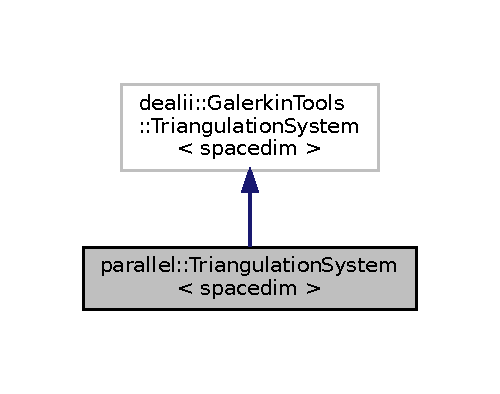
\includegraphics[width=240pt]{classparallel_1_1_triangulation_system__inherit__graph}
\end{center}
\end{figure}


Collaboration diagram for parallel\+::Triangulation\+System$<$ spacedim $>$\+:\nopagebreak
\begin{figure}[H]
\begin{center}
\leavevmode
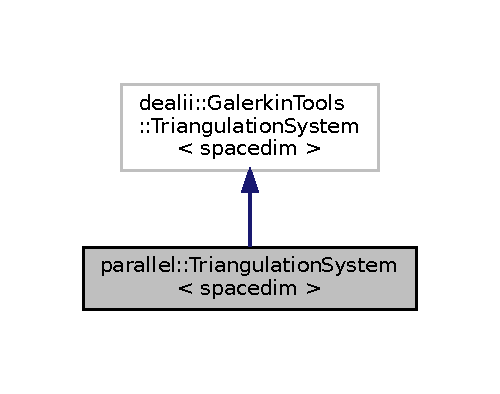
\includegraphics[width=240pt]{classparallel_1_1_triangulation_system__coll__graph}
\end{center}
\end{figure}
\doxysubsection*{Public Member Functions}
\begin{DoxyCompactItemize}
\item 
\mbox{\hyperlink{classparallel_1_1_triangulation_system_a312a7db9393869aa3c9b84b1e316342b}{Triangulation\+System}} (dealii\+::parallel\+::distributed\+::\+Triangulation$<$ spacedim, spacedim $>$ \&tria\+\_\+domain, const bool fix\+\_\+vertex\+\_\+positions=false)
\item 
virtual \mbox{\hyperlink{classparallel_1_1_triangulation_system_ad12682d17e85ee169fd53cdbe0536f16}{$\sim$\+Triangulation\+System}} ()=default
\item 
virtual const dealii\+::parallel\+::distributed\+::\+Triangulation$<$ spacedim, spacedim $>$ \& \mbox{\hyperlink{classparallel_1_1_triangulation_system_a8dfd7da98adf853fd6ec27cbfccec90b}{get\+\_\+triangulation\+\_\+domain}} () const
\item 
virtual const dealii\+::\+Galerkin\+Tools\+::parallel\+::\+Triangulation$<$ spacedim-\/1, spacedim $>$ \& \mbox{\hyperlink{classparallel_1_1_triangulation_system_acaac838c580c71c0152b1eef7c084ebb}{get\+\_\+triangulation\+\_\+interface}} () const
\item 
virtual dealii\+::parallel\+::distributed\+::\+Triangulation$<$ spacedim, spacedim $>$ \& \mbox{\hyperlink{classparallel_1_1_triangulation_system_abadd4ec597f43a8992f6477690c9f6c4}{get\+\_\+triangulation\+\_\+domain}} ()
\item 
virtual dealii\+::\+Galerkin\+Tools\+::parallel\+::\+Triangulation$<$ spacedim-\/1, spacedim $>$ \& \mbox{\hyperlink{classparallel_1_1_triangulation_system_ad5c8bebc3b72cae7e1ec086790b2f76d}{get\+\_\+triangulation\+\_\+interface}} ()
\item 
virtual void \mbox{\hyperlink{classparallel_1_1_triangulation_system_a5a7ef73bec1fbe698480e1bd7c6cd8a7}{close}} ()
\item 
void \mbox{\hyperlink{classparallel_1_1_triangulation_system_a6220dec5dd926987eedf084273062f9c}{write\+\_\+meshes\+\_\+per\+\_\+processor\+\_\+as\+\_\+vtu}} (const std\+::string file\+\_\+name\+\_\+domain, const std\+::string file\+\_\+name\+\_\+interface) const
\item 
virtual std\+::pair$<$ const unsigned int, const unsigned int $>$ \mbox{\hyperlink{classparallel_1_1_triangulation_system_afbde3803f2243308fa33593d6b5f17b4}{get\+\_\+this\+\_\+proc\+\_\+n\+\_\+procs}} () const
\end{DoxyCompactItemize}
\doxysubsection*{Private Member Functions}
\begin{DoxyCompactItemize}
\item 
virtual void \mbox{\hyperlink{classparallel_1_1_triangulation_system_a79e9789e83e12900c85cf8de0644271f}{pre\+\_\+refinement\+\_\+domain}} ()
\item 
virtual void \mbox{\hyperlink{classparallel_1_1_triangulation_system_a951181f2ad877283d458fa19db42efb2}{post\+\_\+refinement\+\_\+domain}} ()
\item 
void \mbox{\hyperlink{classparallel_1_1_triangulation_system_ae214de5a3053ae320a1eb6d879f03b43}{update\+\_\+interface\+\_\+subdomain\+\_\+ids}} () const
\end{DoxyCompactItemize}
\doxysubsection*{Private Attributes}
\begin{DoxyCompactItemize}
\item 
M\+P\+I\+\_\+\+Comm \mbox{\hyperlink{classparallel_1_1_triangulation_system_aff7cdcf04d5a4fb633d714130da893b0}{mpi\+\_\+communicator}}
\end{DoxyCompactItemize}


\doxysubsection{Detailed Description}
\subsubsection*{template$<$unsigned int spacedim$>$\newline
class parallel\+::\+Triangulation\+System$<$ spacedim $>$}

This is the parallel computing equivalent of the class \mbox{\hyperlink{classparallel_1_1_triangulation_system}{Triangulation\+System}} (for general information refer to the documentation of this class).

For the domain triangulation the \textbf{ parallel\+::distributed\+::\+Triangulation} class is used. In contrast, for the interface triangulation the \textbf{ parallel\+::distributed\+::\+Triangulation} class is used, which allows for the necessary manual management of the partitioning of the triangulation.

Regarding ownership of interface cells, the convention used is that the ownership of interface cells is according to the ownership of the underlying domain cells on the minus side of the interface.

In general, the complete coarse domain mesh with all \textbf{ types\+::material\+\_\+id}s, \textbf{ types\+::manifold\+\_\+id}s must be identically defined on each processor (this ensures that no ids are lost during the repartitioning process after mesh refinement).


\begin{DoxyTemplParams}{Template Parameters}
{\em spacedim} & The spatial dimension of the problem. \\
\hline
\end{DoxyTemplParams}


\doxysubsection{Constructor \& Destructor Documentation}
\mbox{\Hypertarget{classparallel_1_1_triangulation_system_a312a7db9393869aa3c9b84b1e316342b}\label{classparallel_1_1_triangulation_system_a312a7db9393869aa3c9b84b1e316342b}} 
\index{parallel::TriangulationSystem$<$ spacedim $>$@{parallel::TriangulationSystem$<$ spacedim $>$}!TriangulationSystem@{TriangulationSystem}}
\index{TriangulationSystem@{TriangulationSystem}!parallel::TriangulationSystem$<$ spacedim $>$@{parallel::TriangulationSystem$<$ spacedim $>$}}
\doxysubsubsection{\texorpdfstring{TriangulationSystem()}{TriangulationSystem()}}
{\footnotesize\ttfamily template$<$unsigned int spacedim$>$ \\
\mbox{\hyperlink{classparallel_1_1_triangulation_system}{parallel\+::\+Triangulation\+System}}$<$ spacedim $>$\+::\mbox{\hyperlink{classparallel_1_1_triangulation_system}{Triangulation\+System}} (\begin{DoxyParamCaption}\item[{dealii\+::parallel\+::distributed\+::\+Triangulation$<$ spacedim, spacedim $>$ \&}]{tria\+\_\+domain,  }\item[{const bool}]{fix\+\_\+vertex\+\_\+positions = {\ttfamily false} }\end{DoxyParamCaption})}

Constructor of the parallel\+::distributed\+::\+Triangulation\+System. Note that the constructor does not copy the {\ttfamily tria\+\_\+domain} object supplied, but rather stores a pointer to it. So do not change it after construction of the parallel\+::distributed\+::\+Triangulation\+System unless you\textquotesingle{}re knowing exactly what you are doing (the only change to the domain triangulation, which is admissible, is mesh refinement). No checking on external changes of the domain triangulation is currently performed and, therefore, doing so may lead to errors which are hard to debug.


\begin{DoxyParams}[1]{Parameters}
\mbox{\texttt{ in}}  & {\em tria\+\_\+domain} & \mbox{\hyperlink{class_triangulation_system_a68bafddc70652cb7c64701c74e86279f}{Triangulation\+System\+::tria\+\_\+domain}}\\
\hline
\mbox{\texttt{ in}}  & {\em fix\+\_\+vertex\+\_\+positions} & \mbox{\hyperlink{class_triangulation_system_a74bfeabee5174d77a8477ba9d2de4813}{Triangulation\+System\+::fix\+\_\+vertex\+\_\+positions}} \\
\hline
\end{DoxyParams}
\mbox{\Hypertarget{classparallel_1_1_triangulation_system_ad12682d17e85ee169fd53cdbe0536f16}\label{classparallel_1_1_triangulation_system_ad12682d17e85ee169fd53cdbe0536f16}} 
\index{parallel::TriangulationSystem$<$ spacedim $>$@{parallel::TriangulationSystem$<$ spacedim $>$}!````~TriangulationSystem@{$\sim$TriangulationSystem}}
\index{````~TriangulationSystem@{$\sim$TriangulationSystem}!parallel::TriangulationSystem$<$ spacedim $>$@{parallel::TriangulationSystem$<$ spacedim $>$}}
\doxysubsubsection{\texorpdfstring{$\sim$TriangulationSystem()}{~TriangulationSystem()}}
{\footnotesize\ttfamily template$<$unsigned int spacedim$>$ \\
virtual \mbox{\hyperlink{classparallel_1_1_triangulation_system}{parallel\+::\+Triangulation\+System}}$<$ spacedim $>$\+::$\sim$\mbox{\hyperlink{classparallel_1_1_triangulation_system}{Triangulation\+System}} (\begin{DoxyParamCaption}{ }\end{DoxyParamCaption})\hspace{0.3cm}{\ttfamily [virtual]}, {\ttfamily [default]}}

Destructor 

\doxysubsection{Member Function Documentation}
\mbox{\Hypertarget{classparallel_1_1_triangulation_system_a5a7ef73bec1fbe698480e1bd7c6cd8a7}\label{classparallel_1_1_triangulation_system_a5a7ef73bec1fbe698480e1bd7c6cd8a7}} 
\index{parallel::TriangulationSystem$<$ spacedim $>$@{parallel::TriangulationSystem$<$ spacedim $>$}!close@{close}}
\index{close@{close}!parallel::TriangulationSystem$<$ spacedim $>$@{parallel::TriangulationSystem$<$ spacedim $>$}}
\doxysubsubsection{\texorpdfstring{close()}{close()}}
{\footnotesize\ttfamily template$<$unsigned int spacedim$>$ \\
virtual void \mbox{\hyperlink{classparallel_1_1_triangulation_system}{parallel\+::\+Triangulation\+System}}$<$ spacedim $>$\+::close (\begin{DoxyParamCaption}{ }\end{DoxyParamCaption})\hspace{0.3cm}{\ttfamily [virtual]}}

Function closing the interface definition. After this function has been called, no modifications to the interface triangulation are possible. This function does the real work of creating the interface triangulation and associating it with the underlying domain triangulation. \mbox{\Hypertarget{classparallel_1_1_triangulation_system_afbde3803f2243308fa33593d6b5f17b4}\label{classparallel_1_1_triangulation_system_afbde3803f2243308fa33593d6b5f17b4}} 
\index{parallel::TriangulationSystem$<$ spacedim $>$@{parallel::TriangulationSystem$<$ spacedim $>$}!get\_this\_proc\_n\_procs@{get\_this\_proc\_n\_procs}}
\index{get\_this\_proc\_n\_procs@{get\_this\_proc\_n\_procs}!parallel::TriangulationSystem$<$ spacedim $>$@{parallel::TriangulationSystem$<$ spacedim $>$}}
\doxysubsubsection{\texorpdfstring{get\_this\_proc\_n\_procs()}{get\_this\_proc\_n\_procs()}}
{\footnotesize\ttfamily template$<$unsigned int spacedim$>$ \\
virtual std\+::pair$<$const unsigned int, const unsigned int$>$ \mbox{\hyperlink{classparallel_1_1_triangulation_system}{parallel\+::\+Triangulation\+System}}$<$ spacedim $>$\+::get\+\_\+this\+\_\+proc\+\_\+n\+\_\+procs (\begin{DoxyParamCaption}{ }\end{DoxyParamCaption}) const\hspace{0.3cm}{\ttfamily [virtual]}}

\begin{DoxyReturn}{Returns}
The number of this processor and the total number of participating processors 
\end{DoxyReturn}
\mbox{\Hypertarget{classparallel_1_1_triangulation_system_abadd4ec597f43a8992f6477690c9f6c4}\label{classparallel_1_1_triangulation_system_abadd4ec597f43a8992f6477690c9f6c4}} 
\index{parallel::TriangulationSystem$<$ spacedim $>$@{parallel::TriangulationSystem$<$ spacedim $>$}!get\_triangulation\_domain@{get\_triangulation\_domain}}
\index{get\_triangulation\_domain@{get\_triangulation\_domain}!parallel::TriangulationSystem$<$ spacedim $>$@{parallel::TriangulationSystem$<$ spacedim $>$}}
\doxysubsubsection{\texorpdfstring{get\_triangulation\_domain()}{get\_triangulation\_domain()}\hspace{0.1cm}{\footnotesize\ttfamily [1/2]}}
{\footnotesize\ttfamily template$<$unsigned int spacedim$>$ \\
virtual dealii\+::parallel\+::distributed\+::\+Triangulation$<$spacedim, spacedim$>$\& \mbox{\hyperlink{classparallel_1_1_triangulation_system}{parallel\+::\+Triangulation\+System}}$<$ spacedim $>$\+::get\+\_\+triangulation\+\_\+domain (\begin{DoxyParamCaption}{ }\end{DoxyParamCaption})\hspace{0.3cm}{\ttfamily [virtual]}}

\begin{DoxyReturn}{Returns}
This returns a reference to the domain triangulation. 
\end{DoxyReturn}
\mbox{\Hypertarget{classparallel_1_1_triangulation_system_a8dfd7da98adf853fd6ec27cbfccec90b}\label{classparallel_1_1_triangulation_system_a8dfd7da98adf853fd6ec27cbfccec90b}} 
\index{parallel::TriangulationSystem$<$ spacedim $>$@{parallel::TriangulationSystem$<$ spacedim $>$}!get\_triangulation\_domain@{get\_triangulation\_domain}}
\index{get\_triangulation\_domain@{get\_triangulation\_domain}!parallel::TriangulationSystem$<$ spacedim $>$@{parallel::TriangulationSystem$<$ spacedim $>$}}
\doxysubsubsection{\texorpdfstring{get\_triangulation\_domain()}{get\_triangulation\_domain()}\hspace{0.1cm}{\footnotesize\ttfamily [2/2]}}
{\footnotesize\ttfamily template$<$unsigned int spacedim$>$ \\
virtual const dealii\+::parallel\+::distributed\+::\+Triangulation$<$spacedim, spacedim$>$\& \mbox{\hyperlink{classparallel_1_1_triangulation_system}{parallel\+::\+Triangulation\+System}}$<$ spacedim $>$\+::get\+\_\+triangulation\+\_\+domain (\begin{DoxyParamCaption}{ }\end{DoxyParamCaption}) const\hspace{0.3cm}{\ttfamily [virtual]}}

\begin{DoxyReturn}{Returns}
This returns a const reference to the domain triangulation. 
\end{DoxyReturn}
\mbox{\Hypertarget{classparallel_1_1_triangulation_system_ad5c8bebc3b72cae7e1ec086790b2f76d}\label{classparallel_1_1_triangulation_system_ad5c8bebc3b72cae7e1ec086790b2f76d}} 
\index{parallel::TriangulationSystem$<$ spacedim $>$@{parallel::TriangulationSystem$<$ spacedim $>$}!get\_triangulation\_interface@{get\_triangulation\_interface}}
\index{get\_triangulation\_interface@{get\_triangulation\_interface}!parallel::TriangulationSystem$<$ spacedim $>$@{parallel::TriangulationSystem$<$ spacedim $>$}}
\doxysubsubsection{\texorpdfstring{get\_triangulation\_interface()}{get\_triangulation\_interface()}\hspace{0.1cm}{\footnotesize\ttfamily [1/2]}}
{\footnotesize\ttfamily template$<$unsigned int spacedim$>$ \\
virtual dealii\+::\+Galerkin\+Tools\+::parallel\+::\+Triangulation$<$spacedim-\/1, spacedim$>$\& \mbox{\hyperlink{classparallel_1_1_triangulation_system}{parallel\+::\+Triangulation\+System}}$<$ spacedim $>$\+::get\+\_\+triangulation\+\_\+interface (\begin{DoxyParamCaption}{ }\end{DoxyParamCaption})\hspace{0.3cm}{\ttfamily [virtual]}}

\begin{DoxyReturn}{Returns}
This returns a reference to the interface triangulation. 
\end{DoxyReturn}
\mbox{\Hypertarget{classparallel_1_1_triangulation_system_acaac838c580c71c0152b1eef7c084ebb}\label{classparallel_1_1_triangulation_system_acaac838c580c71c0152b1eef7c084ebb}} 
\index{parallel::TriangulationSystem$<$ spacedim $>$@{parallel::TriangulationSystem$<$ spacedim $>$}!get\_triangulation\_interface@{get\_triangulation\_interface}}
\index{get\_triangulation\_interface@{get\_triangulation\_interface}!parallel::TriangulationSystem$<$ spacedim $>$@{parallel::TriangulationSystem$<$ spacedim $>$}}
\doxysubsubsection{\texorpdfstring{get\_triangulation\_interface()}{get\_triangulation\_interface()}\hspace{0.1cm}{\footnotesize\ttfamily [2/2]}}
{\footnotesize\ttfamily template$<$unsigned int spacedim$>$ \\
virtual const dealii\+::\+Galerkin\+Tools\+::parallel\+::\+Triangulation$<$spacedim-\/1, spacedim$>$\& \mbox{\hyperlink{classparallel_1_1_triangulation_system}{parallel\+::\+Triangulation\+System}}$<$ spacedim $>$\+::get\+\_\+triangulation\+\_\+interface (\begin{DoxyParamCaption}{ }\end{DoxyParamCaption}) const\hspace{0.3cm}{\ttfamily [virtual]}}

\begin{DoxyReturn}{Returns}
This returns a const reference to the interface triangulation. 
\end{DoxyReturn}
\mbox{\Hypertarget{classparallel_1_1_triangulation_system_a951181f2ad877283d458fa19db42efb2}\label{classparallel_1_1_triangulation_system_a951181f2ad877283d458fa19db42efb2}} 
\index{parallel::TriangulationSystem$<$ spacedim $>$@{parallel::TriangulationSystem$<$ spacedim $>$}!post\_refinement\_domain@{post\_refinement\_domain}}
\index{post\_refinement\_domain@{post\_refinement\_domain}!parallel::TriangulationSystem$<$ spacedim $>$@{parallel::TriangulationSystem$<$ spacedim $>$}}
\doxysubsubsection{\texorpdfstring{post\_refinement\_domain()}{post\_refinement\_domain()}}
{\footnotesize\ttfamily template$<$unsigned int spacedim$>$ \\
virtual void \mbox{\hyperlink{classparallel_1_1_triangulation_system}{parallel\+::\+Triangulation\+System}}$<$ spacedim $>$\+::post\+\_\+refinement\+\_\+domain (\begin{DoxyParamCaption}{ }\end{DoxyParamCaption})\hspace{0.3cm}{\ttfamily [private]}, {\ttfamily [virtual]}}

This internal function takes care that the interface mesh is updated after any refinement/coarsening of the domain cells. The underlying mechanism is that the method is attached to the domain triangulation during construction of the \mbox{\hyperlink{classparallel_1_1_triangulation_system}{Triangulation\+System}}; and it will always be called immediately after the domain mesh has been refined.

\begin{DoxyRefDesc}{Todo}
\item[\mbox{\hyperlink{todo__todo000016}{Todo}}]This function will also have to be involved in the transfer of hidden variables between meshes. However, this is not implemented yet, meaning that hidden variables can currently not be combined with mesh refinement during the computation. \end{DoxyRefDesc}
\mbox{\Hypertarget{classparallel_1_1_triangulation_system_a79e9789e83e12900c85cf8de0644271f}\label{classparallel_1_1_triangulation_system_a79e9789e83e12900c85cf8de0644271f}} 
\index{parallel::TriangulationSystem$<$ spacedim $>$@{parallel::TriangulationSystem$<$ spacedim $>$}!pre\_refinement\_domain@{pre\_refinement\_domain}}
\index{pre\_refinement\_domain@{pre\_refinement\_domain}!parallel::TriangulationSystem$<$ spacedim $>$@{parallel::TriangulationSystem$<$ spacedim $>$}}
\doxysubsubsection{\texorpdfstring{pre\_refinement\_domain()}{pre\_refinement\_domain()}}
{\footnotesize\ttfamily template$<$unsigned int spacedim$>$ \\
virtual void \mbox{\hyperlink{classparallel_1_1_triangulation_system}{parallel\+::\+Triangulation\+System}}$<$ spacedim $>$\+::pre\+\_\+refinement\+\_\+domain (\begin{DoxyParamCaption}{ }\end{DoxyParamCaption})\hspace{0.3cm}{\ttfamily [private]}, {\ttfamily [virtual]}}

In parallel, this function does nothing except triggering the \mbox{\hyperlink{class_triangulation_system_ad3b16b86e7cbe4800fb5a40114cbc5fb}{Triangulation\+System\+::pre\+\_\+refinement()}} signal.

\begin{DoxyRefDesc}{Todo}
\item[\mbox{\hyperlink{todo__todo000015}{Todo}}]This function will have to be involved in the transfer of hidden variables between meshes. However, this is not implemented yet, meaning that hidden variables can currently not be combined with mesh refinement during the computation. \end{DoxyRefDesc}
\mbox{\Hypertarget{classparallel_1_1_triangulation_system_ae214de5a3053ae320a1eb6d879f03b43}\label{classparallel_1_1_triangulation_system_ae214de5a3053ae320a1eb6d879f03b43}} 
\index{parallel::TriangulationSystem$<$ spacedim $>$@{parallel::TriangulationSystem$<$ spacedim $>$}!update\_interface\_subdomain\_ids@{update\_interface\_subdomain\_ids}}
\index{update\_interface\_subdomain\_ids@{update\_interface\_subdomain\_ids}!parallel::TriangulationSystem$<$ spacedim $>$@{parallel::TriangulationSystem$<$ spacedim $>$}}
\doxysubsubsection{\texorpdfstring{update\_interface\_subdomain\_ids()}{update\_interface\_subdomain\_ids()}}
{\footnotesize\ttfamily template$<$unsigned int spacedim$>$ \\
void \mbox{\hyperlink{classparallel_1_1_triangulation_system}{parallel\+::\+Triangulation\+System}}$<$ spacedim $>$\+::update\+\_\+interface\+\_\+subdomain\+\_\+ids (\begin{DoxyParamCaption}{ }\end{DoxyParamCaption}) const\hspace{0.3cm}{\ttfamily [private]}}

This function assigns the interface subdomain ids according to the subdomain ids of the underlying domain cells on the minus side. \mbox{\Hypertarget{classparallel_1_1_triangulation_system_a6220dec5dd926987eedf084273062f9c}\label{classparallel_1_1_triangulation_system_a6220dec5dd926987eedf084273062f9c}} 
\index{parallel::TriangulationSystem$<$ spacedim $>$@{parallel::TriangulationSystem$<$ spacedim $>$}!write\_meshes\_per\_processor\_as\_vtu@{write\_meshes\_per\_processor\_as\_vtu}}
\index{write\_meshes\_per\_processor\_as\_vtu@{write\_meshes\_per\_processor\_as\_vtu}!parallel::TriangulationSystem$<$ spacedim $>$@{parallel::TriangulationSystem$<$ spacedim $>$}}
\doxysubsubsection{\texorpdfstring{write\_meshes\_per\_processor\_as\_vtu()}{write\_meshes\_per\_processor\_as\_vtu()}}
{\footnotesize\ttfamily template$<$unsigned int spacedim$>$ \\
void \mbox{\hyperlink{classparallel_1_1_triangulation_system}{parallel\+::\+Triangulation\+System}}$<$ spacedim $>$\+::write\+\_\+meshes\+\_\+per\+\_\+processor\+\_\+as\+\_\+vtu (\begin{DoxyParamCaption}\item[{const std\+::string}]{file\+\_\+name\+\_\+domain,  }\item[{const std\+::string}]{file\+\_\+name\+\_\+interface }\end{DoxyParamCaption}) const}

Write triangulations in $\ast$.vtu format for each processor, and add a .pvtu file for visualization in Visit or Paraview that describes the collection of $\ast$.vtu files.

Note that the extension .vtu will be added automatically.

If a file name is left empty, the corresponding meshes will not be written.


\begin{DoxyParams}[1]{Parameters}
\mbox{\texttt{ in}}  & {\em file\+\_\+name\+\_\+domain} & file name for the domain triangulation\\
\hline
\mbox{\texttt{ in}}  & {\em file\+\_\+name\+\_\+interface} & file name for the interface triangulation \\
\hline
\end{DoxyParams}


\doxysubsection{Member Data Documentation}
\mbox{\Hypertarget{classparallel_1_1_triangulation_system_aff7cdcf04d5a4fb633d714130da893b0}\label{classparallel_1_1_triangulation_system_aff7cdcf04d5a4fb633d714130da893b0}} 
\index{parallel::TriangulationSystem$<$ spacedim $>$@{parallel::TriangulationSystem$<$ spacedim $>$}!mpi\_communicator@{mpi\_communicator}}
\index{mpi\_communicator@{mpi\_communicator}!parallel::TriangulationSystem$<$ spacedim $>$@{parallel::TriangulationSystem$<$ spacedim $>$}}
\doxysubsubsection{\texorpdfstring{mpi\_communicator}{mpi\_communicator}}
{\footnotesize\ttfamily template$<$unsigned int spacedim$>$ \\
M\+P\+I\+\_\+\+Comm \mbox{\hyperlink{classparallel_1_1_triangulation_system}{parallel\+::\+Triangulation\+System}}$<$ spacedim $>$\+::mpi\+\_\+communicator\hspace{0.3cm}{\ttfamily [private]}}

M\+PI communicator 

The documentation for this class was generated from the following file\+:\begin{DoxyCompactItemize}
\item 
/home/sst/code/\+Galerkin\+Tools/\+Galerkin\+Tools/include/galerkin\+\_\+tools/\mbox{\hyperlink{triangulation__system_8h}{triangulation\+\_\+system.\+h}}\end{DoxyCompactItemize}

\hypertarget{class_triangulation_system}{}\doxysection{Triangulation\+System$<$ spacedim $>$ Class Template Reference}
\label{class_triangulation_system}\index{TriangulationSystem$<$ spacedim $>$@{TriangulationSystem$<$ spacedim $>$}}


{\ttfamily \#include $<$triangulation\+\_\+system.\+h$>$}



Inheritance diagram for Triangulation\+System$<$ spacedim $>$\+:\nopagebreak
\begin{figure}[H]
\begin{center}
\leavevmode
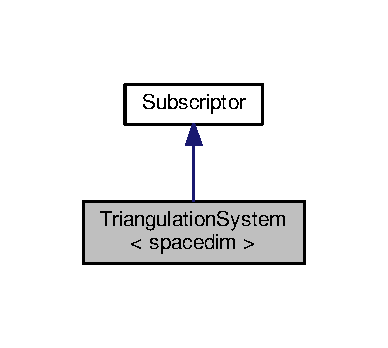
\includegraphics[width=197pt]{class_triangulation_system__inherit__graph}
\end{center}
\end{figure}


Collaboration diagram for Triangulation\+System$<$ spacedim $>$\+:\nopagebreak
\begin{figure}[H]
\begin{center}
\leavevmode
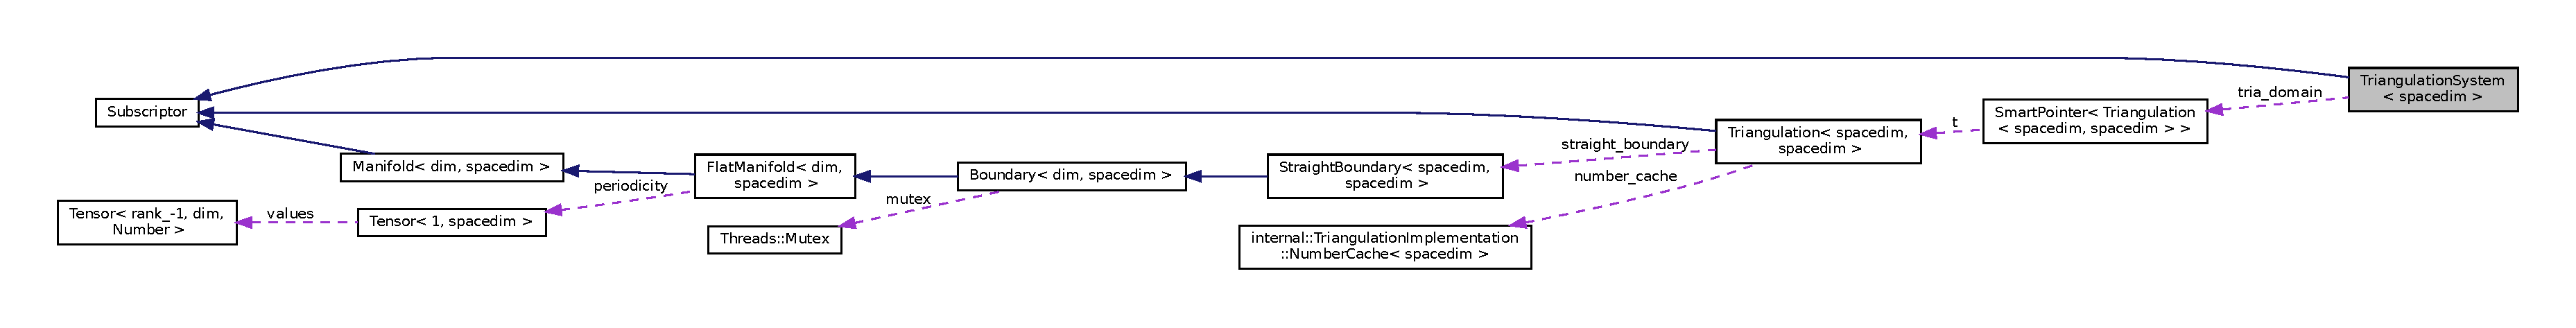
\includegraphics[width=350pt]{class_triangulation_system__coll__graph}
\end{center}
\end{figure}
\doxysubsection*{Public Types}
\begin{DoxyCompactItemize}
\item 
typedef \textbf{ Tria\+Iterator}$<$ \textbf{ Cell\+Accessor}$<$ spacedim-\/1, spacedim $>$ $>$ \mbox{\hyperlink{class_triangulation_system_a1d62a56e335cf19f4a4ec7932fbaef09}{Interface\+Cell}}
\item 
typedef \textbf{ Tria\+Iterator}$<$ \textbf{ Cell\+Accessor}$<$ spacedim, spacedim $>$ $>$ \mbox{\hyperlink{class_triangulation_system_af53de5ec80a16d9cb167660b2832b240}{Domain\+Cell}}
\item 
typedef \textbf{ Tria\+Active\+Iterator}$<$ \textbf{ Cell\+Accessor}$<$ spacedim-\/1, spacedim $>$ $>$ \mbox{\hyperlink{class_triangulation_system_a4c3f97884b5478ebd6771433c5273ac5}{Active\+Interface\+Cell}}
\item 
typedef \textbf{ Tria\+Active\+Iterator}$<$ \textbf{ Cell\+Accessor}$<$ spacedim, spacedim $>$ $>$ \mbox{\hyperlink{class_triangulation_system_a6aa358f6803facdc7e7ee72698a5f4cb}{Active\+Domain\+Cell}}
\end{DoxyCompactItemize}
\doxysubsection*{Public Member Functions}
\begin{DoxyCompactItemize}
\item 
\mbox{\hyperlink{class_triangulation_system_a2d41b2b77cc2835f81a8584ca24dccad}{Triangulation\+System}} (\textbf{ Triangulation}$<$ spacedim, spacedim $>$ \&\mbox{\hyperlink{class_triangulation_system_a68bafddc70652cb7c64701c74e86279f}{tria\+\_\+domain}}, const bool \mbox{\hyperlink{class_triangulation_system_a74bfeabee5174d77a8477ba9d2de4813}{fix\+\_\+vertex\+\_\+positions}}=false)
\item 
virtual \mbox{\hyperlink{class_triangulation_system_a9b0dc550fe1566ab1ba6668a868d0a70}{$\sim$\+Triangulation\+System}} ()
\item 
virtual const \textbf{ Triangulation}$<$ spacedim, spacedim $>$ \& \mbox{\hyperlink{class_triangulation_system_a70637dc46ee4a36433c3ec3c5dc544c5}{get\+\_\+triangulation\+\_\+domain}} () const
\item 
virtual const \textbf{ Triangulation}$<$ spacedim-\/1, spacedim $>$ \& \mbox{\hyperlink{class_triangulation_system_af6c6bc5c73c44896c976bf8e118fa67c}{get\+\_\+triangulation\+\_\+interface}} () const
\item 
virtual \textbf{ Triangulation}$<$ spacedim, spacedim $>$ \& \mbox{\hyperlink{class_triangulation_system_a4c4e1d0589f962d92532586d808c7da2}{get\+\_\+triangulation\+\_\+domain}} ()
\item 
virtual \textbf{ Triangulation}$<$ spacedim-\/1, spacedim $>$ \& \mbox{\hyperlink{class_triangulation_system_a73ef25cdc88395ef6d1ebcf6792cb97f}{get\+\_\+triangulation\+\_\+interface}} ()
\item 
virtual void \mbox{\hyperlink{class_triangulation_system_ad3605f3f59fbd55942288026107c4e6d}{close}} ()
\item 
void \mbox{\hyperlink{class_triangulation_system_a004ced64c3160c7589b6e7bf12f58019}{add\+\_\+interface\+\_\+cell}} (const \mbox{\hyperlink{class_triangulation_system_af53de5ec80a16d9cb167660b2832b240}{Domain\+Cell}} \&domain\+\_\+cell, const unsigned int face, const \textbf{ types\+::material\+\_\+id} \textbf{ material\+\_\+id})
\item 
void \mbox{\hyperlink{class_triangulation_system_a2bb42253dc27cab092c7c76c66b83585}{add\+\_\+interface\+\_\+cells}} (std\+::vector$<$ std\+::tuple$<$ const \mbox{\hyperlink{class_triangulation_system_af53de5ec80a16d9cb167660b2832b240}{Domain\+Cell}}, const unsigned int, const \textbf{ types\+::material\+\_\+id} $>$ $>$ interface\+\_\+cells)
\item 
void \mbox{\hyperlink{class_triangulation_system_a54803f193d6f237b2039ba6f5bca09b9}{set\+\_\+interface\+\_\+manifold}} (const \textbf{ types\+::manifold\+\_\+id} \textbf{ manifold\+\_\+id}, const \textbf{ Manifold}$<$ spacedim-\/1, spacedim $>$ \&manifold)
\item 
void \mbox{\hyperlink{class_triangulation_system_afb5564d01d3914b15b552f95648d231b}{set\+\_\+interface\+\_\+manifolds}} (const std\+::map$<$ \textbf{ types\+::manifold\+\_\+id}, std\+::reference\+\_\+wrapper$<$ const \textbf{ Manifold}$<$ spacedim-\/1, spacedim $>$$>$$>$ manifolds)
\item 
std\+::vector$<$ \mbox{\hyperlink{class_interface_cell_domain_cells}{Interface\+Cell\+Domain\+Cells}}$<$ spacedim $>$ $>$\+::iterator \mbox{\hyperlink{class_triangulation_system_abbbd02a7e813a0604d072480bda93b1a}{interface\+\_\+begin\+\_\+active}} ()
\item 
std\+::vector$<$ \mbox{\hyperlink{class_interface_cell_domain_cells}{Interface\+Cell\+Domain\+Cells}}$<$ spacedim $>$ $>$\+::iterator \mbox{\hyperlink{class_triangulation_system_abcab5ca315d720879468cf92a820c29a}{interface\+\_\+end\+\_\+active}} ()
\item 
const std\+::vector$<$ \mbox{\hyperlink{class_interface_cell_domain_cells}{Interface\+Cell\+Domain\+Cells}}$<$ spacedim $>$ $>$ \& \mbox{\hyperlink{class_triangulation_system_ac46573e9f30edb21ca6f39770ceceaee}{interface\+\_\+active\+\_\+iterators}} () const
\item 
std\+::vector$<$ \mbox{\hyperlink{class_interface_cell_domain_cells}{Interface\+Cell\+Domain\+Cells}}$<$ spacedim $>$ $>$\+::iterator \mbox{\hyperlink{class_triangulation_system_aaf68847ea61f015fce319bb9810833f4}{interface\+\_\+begin\+\_\+coarse}} ()
\item 
std\+::vector$<$ \mbox{\hyperlink{class_interface_cell_domain_cells}{Interface\+Cell\+Domain\+Cells}}$<$ spacedim $>$ $>$\+::iterator \mbox{\hyperlink{class_triangulation_system_a1595839f52f5f5b9d7af31836f9c1f0f}{interface\+\_\+end\+\_\+coarse}} ()
\item 
const std\+::vector$<$ \mbox{\hyperlink{class_interface_cell_domain_cells}{Interface\+Cell\+Domain\+Cells}}$<$ spacedim $>$ $>$ \& \mbox{\hyperlink{class_triangulation_system_afa664696e5d01f0c4b408251311f13b2}{interface\+\_\+coarse\+\_\+iterators}} () const
\item 
void \mbox{\hyperlink{class_triangulation_system_ab8700003a38ead6d2b7cadc896b9c94c}{write\+\_\+triangulations\+\_\+vtk}} (const std\+::string file\+\_\+name\+\_\+domain, const std\+::string file\+\_\+name\+\_\+interface) const
\item 
void \mbox{\hyperlink{class_triangulation_system_a8aa29c77fd798ddd8a5e20806ea21558}{refine\+\_\+global}} (const unsigned int times=1)
\item 
void \mbox{\hyperlink{class_triangulation_system_a62be2563cc8d810a71941e15490f9840}{execute\+\_\+coarsening\+\_\+and\+\_\+refinement}} ()
\item 
bool \mbox{\hyperlink{class_triangulation_system_a6b03827603784e9ce86ddd5484fa52be}{check\+\_\+active\+\_\+interface\+\_\+cell\+\_\+domain\+\_\+cells\+\_\+consistency}} (const double tol=1\textbf{ e}-\/12) const
\item 
virtual std\+::pair$<$ const unsigned int, const unsigned int $>$ \mbox{\hyperlink{class_triangulation_system_a1d468c78ec2c3c57b66bf2c307201eea}{get\+\_\+this\+\_\+proc\+\_\+n\+\_\+procs}} () const
\end{DoxyCompactItemize}
\doxysubsection*{Public Attributes}
\begin{DoxyCompactItemize}
\item 
boost\+::signals2\+::signal$<$ void()$>$ \mbox{\hyperlink{class_triangulation_system_ad3b16b86e7cbe4800fb5a40114cbc5fb}{pre\+\_\+refinement}}
\item 
boost\+::signals2\+::signal$<$ void()$>$ \mbox{\hyperlink{class_triangulation_system_a8813b73cab76c8b77c47c00c39233f76}{post\+\_\+refinement}}
\end{DoxyCompactItemize}
\doxysubsection*{Protected Member Functions}
\begin{DoxyCompactItemize}
\item 
void \mbox{\hyperlink{class_triangulation_system_aee020d825bdf108d69f8e5b71b7ad665}{generate\+\_\+tria\+\_\+interface\+\_\+from\+\_\+tria\+\_\+domain}} ()
\end{DoxyCompactItemize}
\doxysubsection*{Protected Attributes}
\begin{DoxyCompactItemize}
\item 
const \textbf{ Smart\+Pointer}$<$ \textbf{ Triangulation}$<$ spacedim, spacedim $>$ $>$ \mbox{\hyperlink{class_triangulation_system_a68bafddc70652cb7c64701c74e86279f}{tria\+\_\+domain}}
\item 
std\+::unique\+\_\+ptr$<$ \textbf{ Triangulation}$<$ spacedim-\/1, spacedim $>$ $>$ \mbox{\hyperlink{class_triangulation_system_af145fb3f6a3b3ef9ed92111f9fca5b7d}{tria\+\_\+interface}}
\item 
bool \mbox{\hyperlink{class_triangulation_system_aef5ae937cc00b7954357bb8ae88b1f73}{closed}} = false
\end{DoxyCompactItemize}
\doxysubsection*{Private Member Functions}
\begin{DoxyCompactItemize}
\item 
void \mbox{\hyperlink{class_triangulation_system_a4214cf789cf39910305db9fe554249a0}{generate\+\_\+active\+\_\+interface\+\_\+cells\+\_\+domain\+\_\+cells}} (const bool no\+\_\+assert=false)
\item 
void \mbox{\hyperlink{class_triangulation_system_a449457dd44d9c9d9aaa5754532e8537e}{generate\+\_\+active\+\_\+interface\+\_\+cells\+\_\+domain\+\_\+cells\+\_\+recursion}} (const \mbox{\hyperlink{class_triangulation_system_af53de5ec80a16d9cb167660b2832b240}{Domain\+Cell}} \&domain\+\_\+cell, const unsigned int \&face, const \mbox{\hyperlink{class_triangulation_system_a1d62a56e335cf19f4a4ec7932fbaef09}{Interface\+Cell}} \&interface\+\_\+cell, const bool no\+\_\+assert)
\item 
bool \mbox{\hyperlink{class_triangulation_system_a0dfaa2e780dbb0f750b1a85ed9428740}{check\+\_\+material\+\_\+ids\+\_\+recursion}} (const \mbox{\hyperlink{class_triangulation_system_af53de5ec80a16d9cb167660b2832b240}{Domain\+Cell}} \&domain\+\_\+cell) const
\item 
virtual void \mbox{\hyperlink{class_triangulation_system_ae1862e6da3157dc8d539fdc0439e9f48}{pre\+\_\+refinement\+\_\+domain}} ()
\item 
virtual void \mbox{\hyperlink{class_triangulation_system_a8435489384095f687363d200ccfce628}{post\+\_\+refinement\+\_\+domain}} ()
\item 
void \mbox{\hyperlink{class_triangulation_system_aca3dc94f1006a603f56ac12c730ae242}{push\+\_\+tria\+\_\+listeners\+\_\+to\+\_\+end}} ()
\end{DoxyCompactItemize}
\doxysubsection*{Private Attributes}
\begin{DoxyCompactItemize}
\item 
std\+::map$<$ std\+::pair$<$ const \mbox{\hyperlink{class_triangulation_system_af53de5ec80a16d9cb167660b2832b240}{Domain\+Cell}}, const unsigned int $>$, \textbf{ types\+::material\+\_\+id} $>$ \mbox{\hyperlink{class_triangulation_system_a9a14a8a68bda679330a169413f0e2dfb}{coarse\+\_\+domain\+\_\+faces\+\_\+material\+\_\+ids}}
\item 
std\+::map$<$ \textbf{ dealii\+::types\+::manifold\+\_\+id}, const dealii\+::\+Manifold$<$ spacedim-\/1, spacedim $>$ $\ast$ $>$ \mbox{\hyperlink{class_triangulation_system_a130322b74b66f27d8611ce92ad241c6d}{interface\+\_\+manifolds}}
\item 
std\+::vector$<$ \mbox{\hyperlink{class_interface_cell_domain_cells}{Interface\+Cell\+Domain\+Cells}}$<$ spacedim $>$ $>$ \mbox{\hyperlink{class_triangulation_system_a5b909c472fe2508da44e89b017aa146c}{coarse\+\_\+interface\+\_\+cell\+\_\+domain\+\_\+cells}}
\item 
std\+::vector$<$ \mbox{\hyperlink{class_interface_cell_domain_cells}{Interface\+Cell\+Domain\+Cells}}$<$ spacedim $>$ $>$ \mbox{\hyperlink{class_triangulation_system_a516c7a253cefbc5e208714538b21424d}{active\+\_\+interface\+\_\+cell\+\_\+domain\+\_\+cells}}
\item 
std\+::vector$<$ boost\+::signals2\+::connection $>$ \mbox{\hyperlink{class_triangulation_system_a713f97bee5570de1f5571d86a41e83f6}{tria\+\_\+listeners}}
\item 
const bool \mbox{\hyperlink{class_triangulation_system_a74bfeabee5174d77a8477ba9d2de4813}{fix\+\_\+vertex\+\_\+positions}} = false
\end{DoxyCompactItemize}
\doxysubsection*{Friends}
\begin{DoxyCompactItemize}
\item 
{\footnotesize template$<$unsigned int $>$ }\\class \mbox{\hyperlink{class_triangulation_system_af4019c2e39cc934d646aaa35c3c52773}{Assembly\+Helper}}
\end{DoxyCompactItemize}
\doxysubsection*{Additional Inherited Members}


\doxysubsection{Detailed Description}
\subsubsection*{template$<$unsigned int spacedim$>$\newline
class Triangulation\+System$<$ spacedim $>$}

Objects of this class contain all information about the domain and interface mesh and how both of them are related to each other (i.\+e., which domain cell faces underly the interface mesh). They are also used for the actual definition of the interface mesh based on the domain mesh. Moreover, objects of this class are used to ensure that the interface mesh is refined in a consistent way with the domain mesh.

The following general notes apply to domain and interface meshes\+:

(1) The domain mesh may be split into several portions, which are identified by \textbf{ types\+::material\+\_\+id}s. In the same way, the interface mesh may be split into several portions. The domain / interface portions must generally be defined by the coarse mesh cells. I.\+e., child cells must always have the same \textbf{ types\+::material\+\_\+id} as the corresponding coarse cell.

(2) Neighboring domain cells with two different \textbf{ types\+::material\+\_\+id}s will share faces / nodes where they meet if the domain triangulation has been set up accordingly.

(3) Neighboring interface cells with two different \textbf{ types\+::material\+\_\+id}s will not share edges/nodes where they meet. If degrees of freedom are to be shared for these situations, this can currently only be achieved by appropriate constraints.

(4) Boundaries are generally considered as special cases of interfaces. The distinguishing feature of boundaries is just that no mesh exists on one side of the interface (and, therefore, no domain related independent fields live on this side).

(5) An interface mesh must be set up wherever interface related independent fields live and/or Dirichlet type constraints on domain related fields are applied on interfaces using the built in functionality of \mbox{\hyperlink{class_assembly_helper}{Assembly\+Helper}}.

(6) The definition of the interface mesh is done via the domain mesh. In particular, each interface cell is defined by a face of a domain cell. The domain cell used in this process defines the minus side of the interface cell. Generally, only domain cells of the coarse mesh are allowed for the definition of the interfaces. This implies that the coarse domain mesh must be set up before the interface mesh can be defined.

(7) Each interface cell is always refined in the same way as the face of the more refined domain cell adjacent to the interface. Also, it is assumed that refinement of the interface mesh always happens indirectly through refinement of the domain mesh (by the requirement set out before). I.\+e., it is not possible to mark interface cells for refinement. Rather, the adjacent domain cells must be marked for refinement if the interface mesh is to be refined.

(8) At present only isotropic refinement is allowed for. This choice has been made because many important functionalities of the deal.\+II library are based on the very same assumption currently.

(9) The \textbf{ types\+::manifold\+\_\+id}s of interface cells will generally be taken from the \textbf{ types\+::manifold\+\_\+id}s of the coarse mesh domain cell faces underlying the interface cells (on the minus side of the interface).

(10) In order to avoid undefined behavior when the \mbox{\hyperlink{class_triangulation_system}{Triangulation\+System}} is used with an \mbox{\hyperlink{class_assembly_helper}{Assembly\+Helper}} object, the definition of \textbf{ types\+::material\+\_\+id}s, \textbf{ types\+::manifold\+\_\+id}s, etc. should always be done on the coarse domain mesh before the \mbox{\hyperlink{class_triangulation_system}{Triangulation\+System}} is constructed. Also it should be done before any kind of refinement in order to ensure that ids are properly inherited to children (and, therefore, the ids of the refined mesh stay consistent with the coarse mesh).

(11) Due to restrictions in the deal.\+II library, it is presently not allowed for that more than two interface cells share a common edge (and the corresponding nodes). Currently, these situations can only be treated by appropriately \char`\"{}chopping\char`\"{} the interface mesh into different portions (i.\+e., portions with different \textbf{ types\+::material\+\_\+id}s). As described above, this approach will create duplicate edges and nodes where interface cells with different \textbf{ types\+::material\+\_\+id}s meet, meaning that it may be necessary to constrain dofs together on these duplicate edges.

The \mbox{\hyperlink{class_triangulation_system}{Triangulation\+System}} class inherits from \textbf{ Subscriptor} in order to be able to check that \mbox{\hyperlink{class_triangulation_system}{Triangulation\+System}} objects are only destroyed when they are not needed anymore by other objects.


\begin{DoxyTemplParams}{Template Parameters}
{\em spacedim} & The spatial dimension of the problem. \\
\hline
\end{DoxyTemplParams}


\doxysubsection{Member Typedef Documentation}
\mbox{\Hypertarget{class_triangulation_system_a6aa358f6803facdc7e7ee72698a5f4cb}\label{class_triangulation_system_a6aa358f6803facdc7e7ee72698a5f4cb}} 
\index{TriangulationSystem$<$ spacedim $>$@{TriangulationSystem$<$ spacedim $>$}!ActiveDomainCell@{ActiveDomainCell}}
\index{ActiveDomainCell@{ActiveDomainCell}!TriangulationSystem$<$ spacedim $>$@{TriangulationSystem$<$ spacedim $>$}}
\doxysubsubsection{\texorpdfstring{ActiveDomainCell}{ActiveDomainCell}}
{\footnotesize\ttfamily template$<$unsigned int spacedim$>$ \\
typedef \textbf{ Tria\+Active\+Iterator}$<$\textbf{ Cell\+Accessor}$<$spacedim, spacedim$>$ $>$ \mbox{\hyperlink{class_triangulation_system}{Triangulation\+System}}$<$ spacedim $>$\+::\mbox{\hyperlink{class_triangulation_system_a6aa358f6803facdc7e7ee72698a5f4cb}{Active\+Domain\+Cell}}}

A convenience typedef for a deal.\+II \textbf{ Tria\+Active\+Iterator} referring to a domain cell \mbox{\Hypertarget{class_triangulation_system_a4c3f97884b5478ebd6771433c5273ac5}\label{class_triangulation_system_a4c3f97884b5478ebd6771433c5273ac5}} 
\index{TriangulationSystem$<$ spacedim $>$@{TriangulationSystem$<$ spacedim $>$}!ActiveInterfaceCell@{ActiveInterfaceCell}}
\index{ActiveInterfaceCell@{ActiveInterfaceCell}!TriangulationSystem$<$ spacedim $>$@{TriangulationSystem$<$ spacedim $>$}}
\doxysubsubsection{\texorpdfstring{ActiveInterfaceCell}{ActiveInterfaceCell}}
{\footnotesize\ttfamily template$<$unsigned int spacedim$>$ \\
typedef \textbf{ Tria\+Active\+Iterator}$<$\textbf{ Cell\+Accessor}$<$spacedim-\/1, spacedim$>$ $>$ \mbox{\hyperlink{class_triangulation_system}{Triangulation\+System}}$<$ spacedim $>$\+::\mbox{\hyperlink{class_triangulation_system_a4c3f97884b5478ebd6771433c5273ac5}{Active\+Interface\+Cell}}}

A convenience typedef for a deal.\+II \textbf{ Tria\+Active\+Iterator} referring to an interface cell \mbox{\Hypertarget{class_triangulation_system_af53de5ec80a16d9cb167660b2832b240}\label{class_triangulation_system_af53de5ec80a16d9cb167660b2832b240}} 
\index{TriangulationSystem$<$ spacedim $>$@{TriangulationSystem$<$ spacedim $>$}!DomainCell@{DomainCell}}
\index{DomainCell@{DomainCell}!TriangulationSystem$<$ spacedim $>$@{TriangulationSystem$<$ spacedim $>$}}
\doxysubsubsection{\texorpdfstring{DomainCell}{DomainCell}}
{\footnotesize\ttfamily template$<$unsigned int spacedim$>$ \\
typedef \textbf{ Tria\+Iterator}$<$\textbf{ Cell\+Accessor}$<$spacedim, spacedim$>$ $>$ \mbox{\hyperlink{class_triangulation_system}{Triangulation\+System}}$<$ spacedim $>$\+::\mbox{\hyperlink{class_triangulation_system_af53de5ec80a16d9cb167660b2832b240}{Domain\+Cell}}}

A convenience typedef for a deal.\+II \textbf{ Tria\+Iterator} referring to a domain cell \mbox{\Hypertarget{class_triangulation_system_a1d62a56e335cf19f4a4ec7932fbaef09}\label{class_triangulation_system_a1d62a56e335cf19f4a4ec7932fbaef09}} 
\index{TriangulationSystem$<$ spacedim $>$@{TriangulationSystem$<$ spacedim $>$}!InterfaceCell@{InterfaceCell}}
\index{InterfaceCell@{InterfaceCell}!TriangulationSystem$<$ spacedim $>$@{TriangulationSystem$<$ spacedim $>$}}
\doxysubsubsection{\texorpdfstring{InterfaceCell}{InterfaceCell}}
{\footnotesize\ttfamily template$<$unsigned int spacedim$>$ \\
typedef \textbf{ Tria\+Iterator}$<$\textbf{ Cell\+Accessor}$<$spacedim-\/1, spacedim$>$ $>$ \mbox{\hyperlink{class_triangulation_system}{Triangulation\+System}}$<$ spacedim $>$\+::\mbox{\hyperlink{class_triangulation_system_a1d62a56e335cf19f4a4ec7932fbaef09}{Interface\+Cell}}}

A convenience typedef for a deal.\+II \textbf{ Tria\+Iterator} referring to an interface cell 

\doxysubsection{Constructor \& Destructor Documentation}
\mbox{\Hypertarget{class_triangulation_system_a2d41b2b77cc2835f81a8584ca24dccad}\label{class_triangulation_system_a2d41b2b77cc2835f81a8584ca24dccad}} 
\index{TriangulationSystem$<$ spacedim $>$@{TriangulationSystem$<$ spacedim $>$}!TriangulationSystem@{TriangulationSystem}}
\index{TriangulationSystem@{TriangulationSystem}!TriangulationSystem$<$ spacedim $>$@{TriangulationSystem$<$ spacedim $>$}}
\doxysubsubsection{\texorpdfstring{TriangulationSystem()}{TriangulationSystem()}}
{\footnotesize\ttfamily template$<$unsigned int spacedim$>$ \\
\mbox{\hyperlink{class_triangulation_system}{Triangulation\+System}}$<$ spacedim $>$\+::\mbox{\hyperlink{class_triangulation_system}{Triangulation\+System}} (\begin{DoxyParamCaption}\item[{\textbf{ Triangulation}$<$ spacedim, spacedim $>$ \&}]{tria\+\_\+domain,  }\item[{const bool}]{fix\+\_\+vertex\+\_\+positions = {\ttfamily false} }\end{DoxyParamCaption})}

Constructor of the \mbox{\hyperlink{class_triangulation_system}{Triangulation\+System}}. Note that the constructor does not copy the {\ttfamily tria\+\_\+domain} object supplied, but rather stores a pointer to it. So do not change it after construction of the \mbox{\hyperlink{class_triangulation_system}{Triangulation\+System}} unless you\textquotesingle{}re knowing exactly what you are doing (the only change to the domain triangulation, which is admissible, is mesh refinement). No checking on external changes of the domain triangulation is currently performed and, therefore, doing so may lead to errors which are hard to debug.


\begin{DoxyParams}[1]{Parameters}
\mbox{\texttt{ in}}  & {\em tria\+\_\+domain} & \mbox{\hyperlink{class_triangulation_system_a68bafddc70652cb7c64701c74e86279f}{Triangulation\+System\+::tria\+\_\+domain}}\\
\hline
\mbox{\texttt{ in}}  & {\em fix\+\_\+vertex\+\_\+positions} & \mbox{\hyperlink{class_triangulation_system_a74bfeabee5174d77a8477ba9d2de4813}{Triangulation\+System\+::fix\+\_\+vertex\+\_\+positions}} \\
\hline
\end{DoxyParams}
\mbox{\Hypertarget{class_triangulation_system_a9b0dc550fe1566ab1ba6668a868d0a70}\label{class_triangulation_system_a9b0dc550fe1566ab1ba6668a868d0a70}} 
\index{TriangulationSystem$<$ spacedim $>$@{TriangulationSystem$<$ spacedim $>$}!````~TriangulationSystem@{$\sim$TriangulationSystem}}
\index{````~TriangulationSystem@{$\sim$TriangulationSystem}!TriangulationSystem$<$ spacedim $>$@{TriangulationSystem$<$ spacedim $>$}}
\doxysubsubsection{\texorpdfstring{$\sim$TriangulationSystem()}{~TriangulationSystem()}}
{\footnotesize\ttfamily template$<$unsigned int spacedim$>$ \\
virtual \mbox{\hyperlink{class_triangulation_system}{Triangulation\+System}}$<$ spacedim $>$\+::$\sim$\mbox{\hyperlink{class_triangulation_system}{Triangulation\+System}} (\begin{DoxyParamCaption}{ }\end{DoxyParamCaption})\hspace{0.3cm}{\ttfamily [virtual]}}

The destructor of \mbox{\hyperlink{class_triangulation_system}{Triangulation\+System}} essentially checks before destruction that the \mbox{\hyperlink{class_triangulation_system}{Triangulation\+System}} object is not used by other objects. If this is the case, the program will be aborted. 

\doxysubsection{Member Function Documentation}
\mbox{\Hypertarget{class_triangulation_system_a004ced64c3160c7589b6e7bf12f58019}\label{class_triangulation_system_a004ced64c3160c7589b6e7bf12f58019}} 
\index{TriangulationSystem$<$ spacedim $>$@{TriangulationSystem$<$ spacedim $>$}!add\_interface\_cell@{add\_interface\_cell}}
\index{add\_interface\_cell@{add\_interface\_cell}!TriangulationSystem$<$ spacedim $>$@{TriangulationSystem$<$ spacedim $>$}}
\doxysubsubsection{\texorpdfstring{add\_interface\_cell()}{add\_interface\_cell()}}
{\footnotesize\ttfamily template$<$unsigned int spacedim$>$ \\
void \mbox{\hyperlink{class_triangulation_system}{Triangulation\+System}}$<$ spacedim $>$\+::add\+\_\+interface\+\_\+cell (\begin{DoxyParamCaption}\item[{const \mbox{\hyperlink{class_triangulation_system_af53de5ec80a16d9cb167660b2832b240}{Domain\+Cell}} \&}]{domain\+\_\+cell,  }\item[{const unsigned int}]{face,  }\item[{const \textbf{ types\+::material\+\_\+id}}]{material\+\_\+id }\end{DoxyParamCaption})}

This method adds an interface cell to the interface mesh, with the interface cell being defined through the pair ({\ttfamily domain\+\_\+cell}, {\ttfamily face}). The {\ttfamily domain\+\_\+cell} is assumed to be on the minus side of the interface.

Note that this function can only be called before \mbox{\hyperlink{class_triangulation_system_ad3605f3f59fbd55942288026107c4e6d}{Triangulation\+System\+::close()}} has been called.

Note also that the method overwrites previously added cells (i.\+e., if the same combination of cell and face has been added previously, the corresponding {\ttfamily material\+\_\+id} will be overwritten).


\begin{DoxyParams}[1]{Parameters}
\mbox{\texttt{ in}}  & {\em domain\+\_\+cell} & The domain cell underlying the interface cell to be defined\\
\hline
\mbox{\texttt{ in}}  & {\em face} & The face of the domain cell underlying the interface cell to be defined\\
\hline
\mbox{\texttt{ in}}  & {\em material\+\_\+id} & The \textbf{ types\+::material\+\_\+id} which is assigned to the interface cell (thereby deciding to which interface portion the interface cell is linked) \\
\hline
\end{DoxyParams}
\mbox{\Hypertarget{class_triangulation_system_a2bb42253dc27cab092c7c76c66b83585}\label{class_triangulation_system_a2bb42253dc27cab092c7c76c66b83585}} 
\index{TriangulationSystem$<$ spacedim $>$@{TriangulationSystem$<$ spacedim $>$}!add\_interface\_cells@{add\_interface\_cells}}
\index{add\_interface\_cells@{add\_interface\_cells}!TriangulationSystem$<$ spacedim $>$@{TriangulationSystem$<$ spacedim $>$}}
\doxysubsubsection{\texorpdfstring{add\_interface\_cells()}{add\_interface\_cells()}}
{\footnotesize\ttfamily template$<$unsigned int spacedim$>$ \\
void \mbox{\hyperlink{class_triangulation_system}{Triangulation\+System}}$<$ spacedim $>$\+::add\+\_\+interface\+\_\+cells (\begin{DoxyParamCaption}\item[{std\+::vector$<$ std\+::tuple$<$ const \mbox{\hyperlink{class_triangulation_system_af53de5ec80a16d9cb167660b2832b240}{Domain\+Cell}}, const unsigned int, const \textbf{ types\+::material\+\_\+id} $>$ $>$}]{interface\+\_\+cells }\end{DoxyParamCaption})}

Function to add several cells to the interface triangulation at once. This function mainly exists for compatibility with a premature version of the library. Essentially, \mbox{\hyperlink{class_triangulation_system_a004ced64c3160c7589b6e7bf12f58019}{Triangulation\+System\+::add\+\_\+interface\+\_\+cell()}} is called repeatedly for all elements of the input vector {\ttfamily interface\+\_\+cells}.


\begin{DoxyParams}[1]{Parameters}
\mbox{\texttt{ in}}  & {\em interface\+\_\+cells} & A vector defining the interface cell (first in tuple\+: the domain cell underlying the interface cell to be defined; second in tuple\+: the face of the domain cell underlying the interface cell to be defined; third in tuple\+: the \textbf{ types\+::material\+\_\+id} which is assigned to the interface cell ); see also \mbox{\hyperlink{class_triangulation_system_a004ced64c3160c7589b6e7bf12f58019}{Triangulation\+System\+::add\+\_\+interface\+\_\+cell()}} \\
\hline
\end{DoxyParams}
\mbox{\Hypertarget{class_triangulation_system_a6b03827603784e9ce86ddd5484fa52be}\label{class_triangulation_system_a6b03827603784e9ce86ddd5484fa52be}} 
\index{TriangulationSystem$<$ spacedim $>$@{TriangulationSystem$<$ spacedim $>$}!check\_active\_interface\_cell\_domain\_cells\_consistency@{check\_active\_interface\_cell\_domain\_cells\_consistency}}
\index{check\_active\_interface\_cell\_domain\_cells\_consistency@{check\_active\_interface\_cell\_domain\_cells\_consistency}!TriangulationSystem$<$ spacedim $>$@{TriangulationSystem$<$ spacedim $>$}}
\doxysubsubsection{\texorpdfstring{check\_active\_interface\_cell\_domain\_cells\_consistency()}{check\_active\_interface\_cell\_domain\_cells\_consistency()}}
{\footnotesize\ttfamily template$<$unsigned int spacedim$>$ \\
bool \mbox{\hyperlink{class_triangulation_system}{Triangulation\+System}}$<$ spacedim $>$\+::check\+\_\+active\+\_\+interface\+\_\+cell\+\_\+domain\+\_\+cells\+\_\+consistency (\begin{DoxyParamCaption}\item[{const double}]{tol = {\ttfamily 1\textbf{ e}-\/12} }\end{DoxyParamCaption}) const}

This method checks that the active interface cells are properly aligned with the underlying domain cell faces by comparison of cell / face centers.


\begin{DoxyParams}[1]{Parameters}
\mbox{\texttt{ in}}  & {\em tol} & The distance between the center of an interface cell and the center of the underlying domain cell face below which the centers are considered consistent.\\
\hline
\end{DoxyParams}
\begin{DoxyReturn}{Returns}
If {\ttfamily true} is returned, all is in order and the interface mesh is consistent with the domain mesh. If {\ttfamily false} is returned, inconsistencies have been detected. 
\end{DoxyReturn}
\mbox{\Hypertarget{class_triangulation_system_a0dfaa2e780dbb0f750b1a85ed9428740}\label{class_triangulation_system_a0dfaa2e780dbb0f750b1a85ed9428740}} 
\index{TriangulationSystem$<$ spacedim $>$@{TriangulationSystem$<$ spacedim $>$}!check\_material\_ids\_recursion@{check\_material\_ids\_recursion}}
\index{check\_material\_ids\_recursion@{check\_material\_ids\_recursion}!TriangulationSystem$<$ spacedim $>$@{TriangulationSystem$<$ spacedim $>$}}
\doxysubsubsection{\texorpdfstring{check\_material\_ids\_recursion()}{check\_material\_ids\_recursion()}}
{\footnotesize\ttfamily template$<$unsigned int spacedim$>$ \\
bool \mbox{\hyperlink{class_triangulation_system}{Triangulation\+System}}$<$ spacedim $>$\+::check\+\_\+material\+\_\+ids\+\_\+recursion (\begin{DoxyParamCaption}\item[{const \mbox{\hyperlink{class_triangulation_system_af53de5ec80a16d9cb167660b2832b240}{Domain\+Cell}} \&}]{domain\+\_\+cell }\end{DoxyParamCaption}) const\hspace{0.3cm}{\ttfamily [private]}}

This internal auxiliary method is used for checking whether all children of a certain coarse domain cell have the same \textbf{ types\+::material\+\_\+id} as the coarse mother cell. This method is used to assert on the case that the user supplies a refined domain mesh to \mbox{\hyperlink{class_triangulation_system}{Triangulation\+System}}, where the boundaries between different domain portions are not aligned with coarse mesh faces.

The method works its way through the different refinement levels by recursion.


\begin{DoxyParams}[1]{Parameters}
\mbox{\texttt{ in}}  & {\em domain\+\_\+cell} & The mother cell to be checked \\
\hline
\end{DoxyParams}
\begin{DoxyReturn}{Returns}
If {\ttfamily true} is returned, all children of the coarse domain cell have the same \textbf{ types\+::material\+\_\+id} as the coarse mother cell; if {\ttfamily false} is returned, this is not the case. 
\end{DoxyReturn}
\mbox{\Hypertarget{class_triangulation_system_ad3605f3f59fbd55942288026107c4e6d}\label{class_triangulation_system_ad3605f3f59fbd55942288026107c4e6d}} 
\index{TriangulationSystem$<$ spacedim $>$@{TriangulationSystem$<$ spacedim $>$}!close@{close}}
\index{close@{close}!TriangulationSystem$<$ spacedim $>$@{TriangulationSystem$<$ spacedim $>$}}
\doxysubsubsection{\texorpdfstring{close()}{close()}}
{\footnotesize\ttfamily template$<$unsigned int spacedim$>$ \\
virtual void \mbox{\hyperlink{class_triangulation_system}{Triangulation\+System}}$<$ spacedim $>$\+::close (\begin{DoxyParamCaption}{ }\end{DoxyParamCaption})\hspace{0.3cm}{\ttfamily [virtual]}}

Function closing the interface definition. After this function has been called, no modifications to the interface triangulation are possible. This function does the real work of creating the interface triangulation and associating it with the underlying domain triangulation. \mbox{\Hypertarget{class_triangulation_system_a62be2563cc8d810a71941e15490f9840}\label{class_triangulation_system_a62be2563cc8d810a71941e15490f9840}} 
\index{TriangulationSystem$<$ spacedim $>$@{TriangulationSystem$<$ spacedim $>$}!execute\_coarsening\_and\_refinement@{execute\_coarsening\_and\_refinement}}
\index{execute\_coarsening\_and\_refinement@{execute\_coarsening\_and\_refinement}!TriangulationSystem$<$ spacedim $>$@{TriangulationSystem$<$ spacedim $>$}}
\doxysubsubsection{\texorpdfstring{execute\_coarsening\_and\_refinement()}{execute\_coarsening\_and\_refinement()}}
{\footnotesize\ttfamily template$<$unsigned int spacedim$>$ \\
void \mbox{\hyperlink{class_triangulation_system}{Triangulation\+System}}$<$ spacedim $>$\+::execute\+\_\+coarsening\+\_\+and\+\_\+refinement (\begin{DoxyParamCaption}{ }\end{DoxyParamCaption})}

Function to execute coarsening and refinement. This method does nothing but calling the deal.\+II function \mbox{\hyperlink{class_triangulation_system_a62be2563cc8d810a71941e15490f9840}{execute\+\_\+coarsening\+\_\+and\+\_\+refinement()}} on the domain mesh, which will in turn trigger refinement of the interface by \mbox{\hyperlink{class_triangulation_system_ae1862e6da3157dc8d539fdc0439e9f48}{Triangulation\+System\+::pre\+\_\+refinement\+\_\+domain()}} and \mbox{\hyperlink{class_triangulation_system_a8435489384095f687363d200ccfce628}{Triangulation\+System\+::post\+\_\+refinement\+\_\+domain()}}.

\begin{DoxyRefDesc}{Todo}
\item[\mbox{\hyperlink{todo__todo000015}{Todo}}]This function will also have to be involved in the transfer of hidden variables between meshes. However, this is not implemented yet, meaning that hidden variables can currently not be combined with mesh refinement during the computation. \end{DoxyRefDesc}
\mbox{\Hypertarget{class_triangulation_system_a4214cf789cf39910305db9fe554249a0}\label{class_triangulation_system_a4214cf789cf39910305db9fe554249a0}} 
\index{TriangulationSystem$<$ spacedim $>$@{TriangulationSystem$<$ spacedim $>$}!generate\_active\_interface\_cells\_domain\_cells@{generate\_active\_interface\_cells\_domain\_cells}}
\index{generate\_active\_interface\_cells\_domain\_cells@{generate\_active\_interface\_cells\_domain\_cells}!TriangulationSystem$<$ spacedim $>$@{TriangulationSystem$<$ spacedim $>$}}
\doxysubsubsection{\texorpdfstring{generate\_active\_interface\_cells\_domain\_cells()}{generate\_active\_interface\_cells\_domain\_cells()}}
{\footnotesize\ttfamily template$<$unsigned int spacedim$>$ \\
void \mbox{\hyperlink{class_triangulation_system}{Triangulation\+System}}$<$ spacedim $>$\+::generate\+\_\+active\+\_\+interface\+\_\+cells\+\_\+domain\+\_\+cells (\begin{DoxyParamCaption}\item[{const bool}]{no\+\_\+assert = {\ttfamily false} }\end{DoxyParamCaption})\hspace{0.3cm}{\ttfamily [private]}}

This method is used internally to generate / update \mbox{\hyperlink{class_triangulation_system_a516c7a253cefbc5e208714538b21424d}{Triangulation\+System\+::active\+\_\+interface\+\_\+cell\+\_\+domain\+\_\+cells}} after meshing / mesh refinement.


\begin{DoxyParams}[1]{Parameters}
\mbox{\texttt{ in}}  & {\em no\+\_\+assert} & If {\ttfamily no\+\_\+assert} is {\ttfamily true}, no checking is performed whether the interface and domain mesh refinements are consistent. This functionality is necessary when generating {\ttfamily \mbox{\hyperlink{class_triangulation_system_a516c7a253cefbc5e208714538b21424d}{Triangulation\+System\+::active\+\_\+interface\+\_\+cell\+\_\+domain\+\_\+cells}}} after initial meshing because the domain mesh supplied to \mbox{\hyperlink{class_triangulation_system}{Triangulation\+System}} may already be refined. In the latter case, the corresponding interface mesh is refined in several refinement steps until it is consistent with the domain mesh. However, intermediate meshes in this process may not be consistent with the domain mesh and, thus, it must not checked for consistency. \\
\hline
\end{DoxyParams}
\mbox{\Hypertarget{class_triangulation_system_a449457dd44d9c9d9aaa5754532e8537e}\label{class_triangulation_system_a449457dd44d9c9d9aaa5754532e8537e}} 
\index{TriangulationSystem$<$ spacedim $>$@{TriangulationSystem$<$ spacedim $>$}!generate\_active\_interface\_cells\_domain\_cells\_recursion@{generate\_active\_interface\_cells\_domain\_cells\_recursion}}
\index{generate\_active\_interface\_cells\_domain\_cells\_recursion@{generate\_active\_interface\_cells\_domain\_cells\_recursion}!TriangulationSystem$<$ spacedim $>$@{TriangulationSystem$<$ spacedim $>$}}
\doxysubsubsection{\texorpdfstring{generate\_active\_interface\_cells\_domain\_cells\_recursion()}{generate\_active\_interface\_cells\_domain\_cells\_recursion()}}
{\footnotesize\ttfamily template$<$unsigned int spacedim$>$ \\
void \mbox{\hyperlink{class_triangulation_system}{Triangulation\+System}}$<$ spacedim $>$\+::generate\+\_\+active\+\_\+interface\+\_\+cells\+\_\+domain\+\_\+cells\+\_\+recursion (\begin{DoxyParamCaption}\item[{const \mbox{\hyperlink{class_triangulation_system_af53de5ec80a16d9cb167660b2832b240}{Domain\+Cell}} \&}]{domain\+\_\+cell,  }\item[{const unsigned int \&}]{face,  }\item[{const \mbox{\hyperlink{class_triangulation_system_a1d62a56e335cf19f4a4ec7932fbaef09}{Interface\+Cell}} \&}]{interface\+\_\+cell,  }\item[{const bool}]{no\+\_\+assert }\end{DoxyParamCaption})\hspace{0.3cm}{\ttfamily [private]}}

This internal auxiliary method is called by \mbox{\hyperlink{class_triangulation_system_a4214cf789cf39910305db9fe554249a0}{Triangulation\+System\+::generate\+\_\+active\+\_\+interface\+\_\+cells\+\_\+domain\+\_\+cells()}} and does the actual work of generating / updating \mbox{\hyperlink{class_triangulation_system_a516c7a253cefbc5e208714538b21424d}{Triangulation\+System\+::active\+\_\+interface\+\_\+cell\+\_\+domain\+\_\+cells}}. For each pair of ({\ttfamily domain\+\_\+cell}, {\ttfamily face}) defining an interface cell on the coarse level, the method does a recursion through the refinement levels and adds elements to \mbox{\hyperlink{class_triangulation_system_a516c7a253cefbc5e208714538b21424d}{Triangulation\+System\+::active\+\_\+interface\+\_\+cell\+\_\+domain\+\_\+cells}} only at the deepest (i.\+e. active) level.


\begin{DoxyParams}[1]{Parameters}
\mbox{\texttt{ in}}  & {\em domain\+\_\+cell} & Domain cell underlying the interface cell {\ttfamily interface\+\_\+cell} \\
\hline
\mbox{\texttt{ in}}  & {\em face} & Face of {\ttfamily domain\+\_\+cell} underlying interface cell {\ttfamily interface\+\_\+cell} \\
\hline
\mbox{\texttt{ in}}  & {\em interface\+\_\+cell} & The interface cell corresponding to the pair ({\ttfamily domain\+\_\+cell}, {\ttfamily face})\\
\hline
\mbox{\texttt{ in}}  & {\em no\+\_\+assert} & see the documentation of the same parameter in \mbox{\hyperlink{class_triangulation_system_a4214cf789cf39910305db9fe554249a0}{Triangulation\+System\+::generate\+\_\+active\+\_\+interface\+\_\+cells\+\_\+domain\+\_\+cells()}} \\
\hline
\end{DoxyParams}
\mbox{\Hypertarget{class_triangulation_system_aee020d825bdf108d69f8e5b71b7ad665}\label{class_triangulation_system_aee020d825bdf108d69f8e5b71b7ad665}} 
\index{TriangulationSystem$<$ spacedim $>$@{TriangulationSystem$<$ spacedim $>$}!generate\_tria\_interface\_from\_tria\_domain@{generate\_tria\_interface\_from\_tria\_domain}}
\index{generate\_tria\_interface\_from\_tria\_domain@{generate\_tria\_interface\_from\_tria\_domain}!TriangulationSystem$<$ spacedim $>$@{TriangulationSystem$<$ spacedim $>$}}
\doxysubsubsection{\texorpdfstring{generate\_tria\_interface\_from\_tria\_domain()}{generate\_tria\_interface\_from\_tria\_domain()}}
{\footnotesize\ttfamily template$<$unsigned int spacedim$>$ \\
void \mbox{\hyperlink{class_triangulation_system}{Triangulation\+System}}$<$ spacedim $>$\+::generate\+\_\+tria\+\_\+interface\+\_\+from\+\_\+tria\+\_\+domain (\begin{DoxyParamCaption}{ }\end{DoxyParamCaption})\hspace{0.3cm}{\ttfamily [protected]}}

Function generating the interface triangulation from the domain triangulation and setting up \mbox{\hyperlink{class_triangulation_system_a5b909c472fe2508da44e89b017aa146c}{Triangulation\+System\+::coarse\+\_\+interface\+\_\+cell\+\_\+domain\+\_\+cells}} and \mbox{\hyperlink{class_triangulation_system_a516c7a253cefbc5e208714538b21424d}{Triangulation\+System\+::active\+\_\+interface\+\_\+cell\+\_\+domain\+\_\+cells}} \mbox{\Hypertarget{class_triangulation_system_a1d468c78ec2c3c57b66bf2c307201eea}\label{class_triangulation_system_a1d468c78ec2c3c57b66bf2c307201eea}} 
\index{TriangulationSystem$<$ spacedim $>$@{TriangulationSystem$<$ spacedim $>$}!get\_this\_proc\_n\_procs@{get\_this\_proc\_n\_procs}}
\index{get\_this\_proc\_n\_procs@{get\_this\_proc\_n\_procs}!TriangulationSystem$<$ spacedim $>$@{TriangulationSystem$<$ spacedim $>$}}
\doxysubsubsection{\texorpdfstring{get\_this\_proc\_n\_procs()}{get\_this\_proc\_n\_procs()}}
{\footnotesize\ttfamily template$<$unsigned int spacedim$>$ \\
virtual std\+::pair$<$const unsigned int, const unsigned int$>$ \mbox{\hyperlink{class_triangulation_system}{Triangulation\+System}}$<$ spacedim $>$\+::get\+\_\+this\+\_\+proc\+\_\+n\+\_\+procs (\begin{DoxyParamCaption}{ }\end{DoxyParamCaption}) const\hspace{0.3cm}{\ttfamily [virtual]}}

\begin{DoxyReturn}{Returns}
The number of this processor and the total number of participating processors (as this is a sequential triangulation, the result is always (0, 1) 
\end{DoxyReturn}
\mbox{\Hypertarget{class_triangulation_system_a4c4e1d0589f962d92532586d808c7da2}\label{class_triangulation_system_a4c4e1d0589f962d92532586d808c7da2}} 
\index{TriangulationSystem$<$ spacedim $>$@{TriangulationSystem$<$ spacedim $>$}!get\_triangulation\_domain@{get\_triangulation\_domain}}
\index{get\_triangulation\_domain@{get\_triangulation\_domain}!TriangulationSystem$<$ spacedim $>$@{TriangulationSystem$<$ spacedim $>$}}
\doxysubsubsection{\texorpdfstring{get\_triangulation\_domain()}{get\_triangulation\_domain()}\hspace{0.1cm}{\footnotesize\ttfamily [1/2]}}
{\footnotesize\ttfamily template$<$unsigned int spacedim$>$ \\
virtual \textbf{ Triangulation}$<$spacedim, spacedim$>$\& \mbox{\hyperlink{class_triangulation_system}{Triangulation\+System}}$<$ spacedim $>$\+::get\+\_\+triangulation\+\_\+domain (\begin{DoxyParamCaption}{ }\end{DoxyParamCaption})\hspace{0.3cm}{\ttfamily [virtual]}}

\begin{DoxyReturn}{Returns}
This returns a reference to the domain triangulation. 
\end{DoxyReturn}
\mbox{\Hypertarget{class_triangulation_system_a70637dc46ee4a36433c3ec3c5dc544c5}\label{class_triangulation_system_a70637dc46ee4a36433c3ec3c5dc544c5}} 
\index{TriangulationSystem$<$ spacedim $>$@{TriangulationSystem$<$ spacedim $>$}!get\_triangulation\_domain@{get\_triangulation\_domain}}
\index{get\_triangulation\_domain@{get\_triangulation\_domain}!TriangulationSystem$<$ spacedim $>$@{TriangulationSystem$<$ spacedim $>$}}
\doxysubsubsection{\texorpdfstring{get\_triangulation\_domain()}{get\_triangulation\_domain()}\hspace{0.1cm}{\footnotesize\ttfamily [2/2]}}
{\footnotesize\ttfamily template$<$unsigned int spacedim$>$ \\
virtual const \textbf{ Triangulation}$<$spacedim, spacedim$>$\& \mbox{\hyperlink{class_triangulation_system}{Triangulation\+System}}$<$ spacedim $>$\+::get\+\_\+triangulation\+\_\+domain (\begin{DoxyParamCaption}{ }\end{DoxyParamCaption}) const\hspace{0.3cm}{\ttfamily [virtual]}}

\begin{DoxyReturn}{Returns}
This returns a const reference to the domain triangulation. 
\end{DoxyReturn}
\mbox{\Hypertarget{class_triangulation_system_a73ef25cdc88395ef6d1ebcf6792cb97f}\label{class_triangulation_system_a73ef25cdc88395ef6d1ebcf6792cb97f}} 
\index{TriangulationSystem$<$ spacedim $>$@{TriangulationSystem$<$ spacedim $>$}!get\_triangulation\_interface@{get\_triangulation\_interface}}
\index{get\_triangulation\_interface@{get\_triangulation\_interface}!TriangulationSystem$<$ spacedim $>$@{TriangulationSystem$<$ spacedim $>$}}
\doxysubsubsection{\texorpdfstring{get\_triangulation\_interface()}{get\_triangulation\_interface()}\hspace{0.1cm}{\footnotesize\ttfamily [1/2]}}
{\footnotesize\ttfamily template$<$unsigned int spacedim$>$ \\
virtual \textbf{ Triangulation}$<$spacedim-\/1, spacedim$>$\& \mbox{\hyperlink{class_triangulation_system}{Triangulation\+System}}$<$ spacedim $>$\+::get\+\_\+triangulation\+\_\+interface (\begin{DoxyParamCaption}{ }\end{DoxyParamCaption})\hspace{0.3cm}{\ttfamily [virtual]}}

\begin{DoxyReturn}{Returns}
This returns a reference to the interface triangulation. 
\end{DoxyReturn}
\mbox{\Hypertarget{class_triangulation_system_af6c6bc5c73c44896c976bf8e118fa67c}\label{class_triangulation_system_af6c6bc5c73c44896c976bf8e118fa67c}} 
\index{TriangulationSystem$<$ spacedim $>$@{TriangulationSystem$<$ spacedim $>$}!get\_triangulation\_interface@{get\_triangulation\_interface}}
\index{get\_triangulation\_interface@{get\_triangulation\_interface}!TriangulationSystem$<$ spacedim $>$@{TriangulationSystem$<$ spacedim $>$}}
\doxysubsubsection{\texorpdfstring{get\_triangulation\_interface()}{get\_triangulation\_interface()}\hspace{0.1cm}{\footnotesize\ttfamily [2/2]}}
{\footnotesize\ttfamily template$<$unsigned int spacedim$>$ \\
virtual const \textbf{ Triangulation}$<$spacedim-\/1, spacedim$>$\& \mbox{\hyperlink{class_triangulation_system}{Triangulation\+System}}$<$ spacedim $>$\+::get\+\_\+triangulation\+\_\+interface (\begin{DoxyParamCaption}{ }\end{DoxyParamCaption}) const\hspace{0.3cm}{\ttfamily [virtual]}}

\begin{DoxyReturn}{Returns}
This returns a const reference to the interface triangulation. 
\end{DoxyReturn}
\mbox{\Hypertarget{class_triangulation_system_ac46573e9f30edb21ca6f39770ceceaee}\label{class_triangulation_system_ac46573e9f30edb21ca6f39770ceceaee}} 
\index{TriangulationSystem$<$ spacedim $>$@{TriangulationSystem$<$ spacedim $>$}!interface\_active\_iterators@{interface\_active\_iterators}}
\index{interface\_active\_iterators@{interface\_active\_iterators}!TriangulationSystem$<$ spacedim $>$@{TriangulationSystem$<$ spacedim $>$}}
\doxysubsubsection{\texorpdfstring{interface\_active\_iterators()}{interface\_active\_iterators()}}
{\footnotesize\ttfamily template$<$unsigned int spacedim$>$ \\
const std\+::vector$<$\mbox{\hyperlink{class_interface_cell_domain_cells}{Interface\+Cell\+Domain\+Cells}}$<$spacedim$>$ $>$\& \mbox{\hyperlink{class_triangulation_system}{Triangulation\+System}}$<$ spacedim $>$\+::interface\+\_\+active\+\_\+iterators (\begin{DoxyParamCaption}{ }\end{DoxyParamCaption}) const}

\begin{DoxyReturn}{Returns}
This returns a const reference to \mbox{\hyperlink{class_triangulation_system_a516c7a253cefbc5e208714538b21424d}{Triangulation\+System\+::active\+\_\+interface\+\_\+cell\+\_\+domain\+\_\+cells}}, which is essentially be meant for range based loops instead of using the functions \mbox{\hyperlink{class_triangulation_system_abbbd02a7e813a0604d072480bda93b1a}{Triangulation\+System\+::interface\+\_\+begin\+\_\+active()}} and \mbox{\hyperlink{class_triangulation_system_abcab5ca315d720879468cf92a820c29a}{Triangulation\+System\+::interface\+\_\+end\+\_\+active()}} (hence the name of the function). 
\end{DoxyReturn}
\mbox{\Hypertarget{class_triangulation_system_abbbd02a7e813a0604d072480bda93b1a}\label{class_triangulation_system_abbbd02a7e813a0604d072480bda93b1a}} 
\index{TriangulationSystem$<$ spacedim $>$@{TriangulationSystem$<$ spacedim $>$}!interface\_begin\_active@{interface\_begin\_active}}
\index{interface\_begin\_active@{interface\_begin\_active}!TriangulationSystem$<$ spacedim $>$@{TriangulationSystem$<$ spacedim $>$}}
\doxysubsubsection{\texorpdfstring{interface\_begin\_active()}{interface\_begin\_active()}}
{\footnotesize\ttfamily template$<$unsigned int spacedim$>$ \\
std\+::vector$<$\mbox{\hyperlink{class_interface_cell_domain_cells}{Interface\+Cell\+Domain\+Cells}}$<$spacedim$>$ $>$\+::iterator \mbox{\hyperlink{class_triangulation_system}{Triangulation\+System}}$<$ spacedim $>$\+::interface\+\_\+begin\+\_\+active (\begin{DoxyParamCaption}{ }\end{DoxyParamCaption})}

\begin{DoxyReturn}{Returns}
An iterator to the first active interface cell. Note that this is not a deal.\+II iterator. Rather, it is an iterator to the first element in \mbox{\hyperlink{class_triangulation_system_a516c7a253cefbc5e208714538b21424d}{Triangulation\+System\+::active\+\_\+interface\+\_\+cell\+\_\+domain\+\_\+cells}}. However, through the returned iterator, deal.\+II iterators to the interface cells and adjacent domain cells can be obtained. 
\end{DoxyReturn}
\mbox{\Hypertarget{class_triangulation_system_aaf68847ea61f015fce319bb9810833f4}\label{class_triangulation_system_aaf68847ea61f015fce319bb9810833f4}} 
\index{TriangulationSystem$<$ spacedim $>$@{TriangulationSystem$<$ spacedim $>$}!interface\_begin\_coarse@{interface\_begin\_coarse}}
\index{interface\_begin\_coarse@{interface\_begin\_coarse}!TriangulationSystem$<$ spacedim $>$@{TriangulationSystem$<$ spacedim $>$}}
\doxysubsubsection{\texorpdfstring{interface\_begin\_coarse()}{interface\_begin\_coarse()}}
{\footnotesize\ttfamily template$<$unsigned int spacedim$>$ \\
std\+::vector$<$\mbox{\hyperlink{class_interface_cell_domain_cells}{Interface\+Cell\+Domain\+Cells}}$<$spacedim$>$ $>$\+::iterator \mbox{\hyperlink{class_triangulation_system}{Triangulation\+System}}$<$ spacedim $>$\+::interface\+\_\+begin\+\_\+coarse (\begin{DoxyParamCaption}{ }\end{DoxyParamCaption})}

\begin{DoxyReturn}{Returns}
An iterator to the first coarse interface cell. Note that this is not a deal.\+II iterator. Rather, it is an iterator to the first element in \mbox{\hyperlink{class_triangulation_system_a5b909c472fe2508da44e89b017aa146c}{Triangulation\+System\+::coarse\+\_\+interface\+\_\+cell\+\_\+domain\+\_\+cells}}. However, through the returned iterator, deal.\+II iterators to the interface cells and adjacent domain cells can be obtained. 
\end{DoxyReturn}
\mbox{\Hypertarget{class_triangulation_system_afa664696e5d01f0c4b408251311f13b2}\label{class_triangulation_system_afa664696e5d01f0c4b408251311f13b2}} 
\index{TriangulationSystem$<$ spacedim $>$@{TriangulationSystem$<$ spacedim $>$}!interface\_coarse\_iterators@{interface\_coarse\_iterators}}
\index{interface\_coarse\_iterators@{interface\_coarse\_iterators}!TriangulationSystem$<$ spacedim $>$@{TriangulationSystem$<$ spacedim $>$}}
\doxysubsubsection{\texorpdfstring{interface\_coarse\_iterators()}{interface\_coarse\_iterators()}}
{\footnotesize\ttfamily template$<$unsigned int spacedim$>$ \\
const std\+::vector$<$\mbox{\hyperlink{class_interface_cell_domain_cells}{Interface\+Cell\+Domain\+Cells}}$<$spacedim$>$ $>$\& \mbox{\hyperlink{class_triangulation_system}{Triangulation\+System}}$<$ spacedim $>$\+::interface\+\_\+coarse\+\_\+iterators (\begin{DoxyParamCaption}{ }\end{DoxyParamCaption}) const}

\begin{DoxyReturn}{Returns}
This returns a const reference to \mbox{\hyperlink{class_triangulation_system_a5b909c472fe2508da44e89b017aa146c}{Triangulation\+System\+::coarse\+\_\+interface\+\_\+cell\+\_\+domain\+\_\+cells}}, which is essentially be meant for range based loops instead of using the functions \mbox{\hyperlink{class_triangulation_system_aaf68847ea61f015fce319bb9810833f4}{Triangulation\+System\+::interface\+\_\+begin\+\_\+coarse()}} and \mbox{\hyperlink{class_triangulation_system_a1595839f52f5f5b9d7af31836f9c1f0f}{Triangulation\+System\+::interface\+\_\+end\+\_\+coarse()}} (hence the name of the function). 
\end{DoxyReturn}
\mbox{\Hypertarget{class_triangulation_system_abcab5ca315d720879468cf92a820c29a}\label{class_triangulation_system_abcab5ca315d720879468cf92a820c29a}} 
\index{TriangulationSystem$<$ spacedim $>$@{TriangulationSystem$<$ spacedim $>$}!interface\_end\_active@{interface\_end\_active}}
\index{interface\_end\_active@{interface\_end\_active}!TriangulationSystem$<$ spacedim $>$@{TriangulationSystem$<$ spacedim $>$}}
\doxysubsubsection{\texorpdfstring{interface\_end\_active()}{interface\_end\_active()}}
{\footnotesize\ttfamily template$<$unsigned int spacedim$>$ \\
std\+::vector$<$\mbox{\hyperlink{class_interface_cell_domain_cells}{Interface\+Cell\+Domain\+Cells}}$<$spacedim$>$ $>$\+::iterator \mbox{\hyperlink{class_triangulation_system}{Triangulation\+System}}$<$ spacedim $>$\+::interface\+\_\+end\+\_\+active (\begin{DoxyParamCaption}{ }\end{DoxyParamCaption})}

\begin{DoxyReturn}{Returns}
An iterator to past the last active interface cell. Note that this is not a deal.\+II iterator. Rather, it is an iterator to the past the end element in \mbox{\hyperlink{class_triangulation_system_a516c7a253cefbc5e208714538b21424d}{Triangulation\+System\+::active\+\_\+interface\+\_\+cell\+\_\+domain\+\_\+cells}}. 
\end{DoxyReturn}
\mbox{\Hypertarget{class_triangulation_system_a1595839f52f5f5b9d7af31836f9c1f0f}\label{class_triangulation_system_a1595839f52f5f5b9d7af31836f9c1f0f}} 
\index{TriangulationSystem$<$ spacedim $>$@{TriangulationSystem$<$ spacedim $>$}!interface\_end\_coarse@{interface\_end\_coarse}}
\index{interface\_end\_coarse@{interface\_end\_coarse}!TriangulationSystem$<$ spacedim $>$@{TriangulationSystem$<$ spacedim $>$}}
\doxysubsubsection{\texorpdfstring{interface\_end\_coarse()}{interface\_end\_coarse()}}
{\footnotesize\ttfamily template$<$unsigned int spacedim$>$ \\
std\+::vector$<$\mbox{\hyperlink{class_interface_cell_domain_cells}{Interface\+Cell\+Domain\+Cells}}$<$spacedim$>$ $>$\+::iterator \mbox{\hyperlink{class_triangulation_system}{Triangulation\+System}}$<$ spacedim $>$\+::interface\+\_\+end\+\_\+coarse (\begin{DoxyParamCaption}{ }\end{DoxyParamCaption})}

\begin{DoxyReturn}{Returns}
An iterator to past the last coarse interface cell. Note that this is not a deal.\+II iterator. Rather, it is an iterator to the past the end element in \mbox{\hyperlink{class_triangulation_system_a5b909c472fe2508da44e89b017aa146c}{Triangulation\+System\+::coarse\+\_\+interface\+\_\+cell\+\_\+domain\+\_\+cells}}. 
\end{DoxyReturn}
\mbox{\Hypertarget{class_triangulation_system_a8435489384095f687363d200ccfce628}\label{class_triangulation_system_a8435489384095f687363d200ccfce628}} 
\index{TriangulationSystem$<$ spacedim $>$@{TriangulationSystem$<$ spacedim $>$}!post\_refinement\_domain@{post\_refinement\_domain}}
\index{post\_refinement\_domain@{post\_refinement\_domain}!TriangulationSystem$<$ spacedim $>$@{TriangulationSystem$<$ spacedim $>$}}
\doxysubsubsection{\texorpdfstring{post\_refinement\_domain()}{post\_refinement\_domain()}}
{\footnotesize\ttfamily template$<$unsigned int spacedim$>$ \\
virtual void \mbox{\hyperlink{class_triangulation_system}{Triangulation\+System}}$<$ spacedim $>$\+::post\+\_\+refinement\+\_\+domain (\begin{DoxyParamCaption}{ }\end{DoxyParamCaption})\hspace{0.3cm}{\ttfamily [private]}, {\ttfamily [virtual]}}

This internal function takes care that the interface cells are refined/coarsened after any refinement of the domain cells. The underlying mechanism is that the method is attached to the domain triangulation during construction of the \mbox{\hyperlink{class_triangulation_system}{Triangulation\+System}}; and it will always be called immediately after the domain mesh has been refined.

\begin{DoxyRefDesc}{Todo}
\item[\mbox{\hyperlink{todo__todo000014}{Todo}}]This function will also have to be involved in the transfer of hidden variables between meshes. However, this is not implemented yet, meaning that hidden variables can currently not be combined with mesh refinement during the computation. \end{DoxyRefDesc}
\mbox{\Hypertarget{class_triangulation_system_ae1862e6da3157dc8d539fdc0439e9f48}\label{class_triangulation_system_ae1862e6da3157dc8d539fdc0439e9f48}} 
\index{TriangulationSystem$<$ spacedim $>$@{TriangulationSystem$<$ spacedim $>$}!pre\_refinement\_domain@{pre\_refinement\_domain}}
\index{pre\_refinement\_domain@{pre\_refinement\_domain}!TriangulationSystem$<$ spacedim $>$@{TriangulationSystem$<$ spacedim $>$}}
\doxysubsubsection{\texorpdfstring{pre\_refinement\_domain()}{pre\_refinement\_domain()}}
{\footnotesize\ttfamily template$<$unsigned int spacedim$>$ \\
virtual void \mbox{\hyperlink{class_triangulation_system}{Triangulation\+System}}$<$ spacedim $>$\+::pre\+\_\+refinement\+\_\+domain (\begin{DoxyParamCaption}{ }\end{DoxyParamCaption})\hspace{0.3cm}{\ttfamily [private]}, {\ttfamily [virtual]}}

This function takes care that the interface cells are appropriately marked for refinement/coarsening if the domain mesh is going to be refined. The underlying mechanism is that the method is attached to the domain triangulation during construction of the \mbox{\hyperlink{class_triangulation_system}{Triangulation\+System}}; and it will always be called immediately before the domain mesh is actually refined (i.\+e., after all refinement flags of the domain mesh have been checked for consistency and mesh smoothing has been performed).

\begin{DoxyRefDesc}{Todo}
\item[\mbox{\hyperlink{todo__todo000013}{Todo}}]This function will also have to be involved in the transfer of hidden variables between meshes. However, this is not implemented yet, meaning that hidden variables can currently not be combined with mesh refinement during the computation. \end{DoxyRefDesc}
\mbox{\Hypertarget{class_triangulation_system_aca3dc94f1006a603f56ac12c730ae242}\label{class_triangulation_system_aca3dc94f1006a603f56ac12c730ae242}} 
\index{TriangulationSystem$<$ spacedim $>$@{TriangulationSystem$<$ spacedim $>$}!push\_tria\_listeners\_to\_end@{push\_tria\_listeners\_to\_end}}
\index{push\_tria\_listeners\_to\_end@{push\_tria\_listeners\_to\_end}!TriangulationSystem$<$ spacedim $>$@{TriangulationSystem$<$ spacedim $>$}}
\doxysubsubsection{\texorpdfstring{push\_tria\_listeners\_to\_end()}{push\_tria\_listeners\_to\_end()}}
{\footnotesize\ttfamily template$<$unsigned int spacedim$>$ \\
void \mbox{\hyperlink{class_triangulation_system}{Triangulation\+System}}$<$ spacedim $>$\+::push\+\_\+tria\+\_\+listeners\+\_\+to\+\_\+end (\begin{DoxyParamCaption}{ }\end{DoxyParamCaption})\hspace{0.3cm}{\ttfamily [private]}}

This function disconnects all listeners in \mbox{\hyperlink{class_triangulation_system_a713f97bee5570de1f5571d86a41e83f6}{Triangulation\+System\+::tria\+\_\+listeners}} and reconnects them. This provides a mechanism to make sure that the functions related to \mbox{\hyperlink{class_triangulation_system_a713f97bee5570de1f5571d86a41e83f6}{Triangulation\+System\+::tria\+\_\+listeners}} are called as the very last step. This function is for internal use by \mbox{\hyperlink{class_assembly_helper}{Assembly\+Helper}}. \mbox{\Hypertarget{class_triangulation_system_a8aa29c77fd798ddd8a5e20806ea21558}\label{class_triangulation_system_a8aa29c77fd798ddd8a5e20806ea21558}} 
\index{TriangulationSystem$<$ spacedim $>$@{TriangulationSystem$<$ spacedim $>$}!refine\_global@{refine\_global}}
\index{refine\_global@{refine\_global}!TriangulationSystem$<$ spacedim $>$@{TriangulationSystem$<$ spacedim $>$}}
\doxysubsubsection{\texorpdfstring{refine\_global()}{refine\_global()}}
{\footnotesize\ttfamily template$<$unsigned int spacedim$>$ \\
void \mbox{\hyperlink{class_triangulation_system}{Triangulation\+System}}$<$ spacedim $>$\+::refine\+\_\+global (\begin{DoxyParamCaption}\item[{const unsigned int}]{times = {\ttfamily 1} }\end{DoxyParamCaption})}

Function for global mesh refinement. This method does nothing but calling the deal.\+II function \mbox{\hyperlink{class_triangulation_system_a8aa29c77fd798ddd8a5e20806ea21558}{refine\+\_\+global()}} on the domain mesh, which will in turn trigger refinement of the interface by \mbox{\hyperlink{class_triangulation_system_ae1862e6da3157dc8d539fdc0439e9f48}{Triangulation\+System\+::pre\+\_\+refinement\+\_\+domain()}} and \mbox{\hyperlink{class_triangulation_system_a8435489384095f687363d200ccfce628}{Triangulation\+System\+::post\+\_\+refinement\+\_\+domain()}}. \mbox{\Hypertarget{class_triangulation_system_a54803f193d6f237b2039ba6f5bca09b9}\label{class_triangulation_system_a54803f193d6f237b2039ba6f5bca09b9}} 
\index{TriangulationSystem$<$ spacedim $>$@{TriangulationSystem$<$ spacedim $>$}!set\_interface\_manifold@{set\_interface\_manifold}}
\index{set\_interface\_manifold@{set\_interface\_manifold}!TriangulationSystem$<$ spacedim $>$@{TriangulationSystem$<$ spacedim $>$}}
\doxysubsubsection{\texorpdfstring{set\_interface\_manifold()}{set\_interface\_manifold()}}
{\footnotesize\ttfamily template$<$unsigned int spacedim$>$ \\
void \mbox{\hyperlink{class_triangulation_system}{Triangulation\+System}}$<$ spacedim $>$\+::set\+\_\+interface\+\_\+manifold (\begin{DoxyParamCaption}\item[{const \textbf{ types\+::manifold\+\_\+id}}]{manifold\+\_\+id,  }\item[{const \textbf{ Manifold}$<$ spacedim-\/1, spacedim $>$ \&}]{manifold }\end{DoxyParamCaption})}

Attach a manifold to the interface (note that the \textbf{ types\+::manifold\+\_\+id}s of interface cells will generally be taken from the \textbf{ types\+::manifold\+\_\+id} of the coarse mesh domain cell faces underlying the interface cells on the minus side of the interface). By attaching appropriate manifolds to the interface, it can be ensured that the refinement of the interface triangulation stays geometrically consistent with the refinement of the underlying domain cells. To achieve the latter, the codim 1 equivalents of the manifolds used by the domain triangulation must be added with the same \textbf{ types\+::manifold\+\_\+id}s.

This method is necessary because there is currently no way to directly obtain the codim 1 equivalent from a manifold used on the domain.


\begin{DoxyParams}[1]{Parameters}
\mbox{\texttt{ in}}  & {\em manifold\+\_\+id} & The \textbf{ types\+::manifold\+\_\+id} with which {\ttfamily manifold} will be associated\\
\hline
\mbox{\texttt{ in}}  & {\em manifold} & Reference to the codim 1 manifold to be used \\
\hline
\end{DoxyParams}
\mbox{\Hypertarget{class_triangulation_system_afb5564d01d3914b15b552f95648d231b}\label{class_triangulation_system_afb5564d01d3914b15b552f95648d231b}} 
\index{TriangulationSystem$<$ spacedim $>$@{TriangulationSystem$<$ spacedim $>$}!set\_interface\_manifolds@{set\_interface\_manifolds}}
\index{set\_interface\_manifolds@{set\_interface\_manifolds}!TriangulationSystem$<$ spacedim $>$@{TriangulationSystem$<$ spacedim $>$}}
\doxysubsubsection{\texorpdfstring{set\_interface\_manifolds()}{set\_interface\_manifolds()}}
{\footnotesize\ttfamily template$<$unsigned int spacedim$>$ \\
void \mbox{\hyperlink{class_triangulation_system}{Triangulation\+System}}$<$ spacedim $>$\+::set\+\_\+interface\+\_\+manifolds (\begin{DoxyParamCaption}\item[{const std\+::map$<$ \textbf{ types\+::manifold\+\_\+id}, std\+::reference\+\_\+wrapper$<$ const \textbf{ Manifold}$<$ spacedim-\/1, spacedim $>$$>$$>$}]{manifolds }\end{DoxyParamCaption})}

Function to add several manifolds to the interface triangulation at once. This function mainly exists for compatibility with a premature version of the library. Essentially, \mbox{\hyperlink{class_triangulation_system_a54803f193d6f237b2039ba6f5bca09b9}{Triangulation\+System\+::set\+\_\+interface\+\_\+manifold()}} is called repeatedly for all elements of the input vector {\ttfamily manifolds}.


\begin{DoxyParams}[1]{Parameters}
\mbox{\texttt{ in}}  & {\em manifolds} & A map between \textbf{ types\+::manifold\+\_\+id}s and corresponding manifold objects \\
\hline
\end{DoxyParams}
\mbox{\Hypertarget{class_triangulation_system_ab8700003a38ead6d2b7cadc896b9c94c}\label{class_triangulation_system_ab8700003a38ead6d2b7cadc896b9c94c}} 
\index{TriangulationSystem$<$ spacedim $>$@{TriangulationSystem$<$ spacedim $>$}!write\_triangulations\_vtk@{write\_triangulations\_vtk}}
\index{write\_triangulations\_vtk@{write\_triangulations\_vtk}!TriangulationSystem$<$ spacedim $>$@{TriangulationSystem$<$ spacedim $>$}}
\doxysubsubsection{\texorpdfstring{write\_triangulations\_vtk()}{write\_triangulations\_vtk()}}
{\footnotesize\ttfamily template$<$unsigned int spacedim$>$ \\
void \mbox{\hyperlink{class_triangulation_system}{Triangulation\+System}}$<$ spacedim $>$\+::write\+\_\+triangulations\+\_\+vtk (\begin{DoxyParamCaption}\item[{const std\+::string}]{file\+\_\+name\+\_\+domain,  }\item[{const std\+::string}]{file\+\_\+name\+\_\+interface }\end{DoxyParamCaption}) const}

A convenience method writing the domain and interface triangulations to vtk files. Note that the extension .vtk will not be added automatically. So, it has to be included in the file names.

If a file name is left empty, the corresponding mesh will not be written.


\begin{DoxyParams}[1]{Parameters}
\mbox{\texttt{ in}}  & {\em file\+\_\+name\+\_\+domain} & file name for the domain triangulation\\
\hline
\mbox{\texttt{ in}}  & {\em file\+\_\+name\+\_\+interface} & file name for the interface triangulation \\
\hline
\end{DoxyParams}


\doxysubsection{Friends And Related Function Documentation}
\mbox{\Hypertarget{class_triangulation_system_af4019c2e39cc934d646aaa35c3c52773}\label{class_triangulation_system_af4019c2e39cc934d646aaa35c3c52773}} 
\index{TriangulationSystem$<$ spacedim $>$@{TriangulationSystem$<$ spacedim $>$}!AssemblyHelper@{AssemblyHelper}}
\index{AssemblyHelper@{AssemblyHelper}!TriangulationSystem$<$ spacedim $>$@{TriangulationSystem$<$ spacedim $>$}}
\doxysubsubsection{\texorpdfstring{AssemblyHelper}{AssemblyHelper}}
{\footnotesize\ttfamily template$<$unsigned int spacedim$>$ \\
template$<$unsigned int $>$ \\
friend class \mbox{\hyperlink{class_assembly_helper}{Assembly\+Helper}}\hspace{0.3cm}{\ttfamily [friend]}}

Make \mbox{\hyperlink{class_assembly_helper}{Assembly\+Helper}} a friend to simplify some procedures 

\doxysubsection{Member Data Documentation}
\mbox{\Hypertarget{class_triangulation_system_a516c7a253cefbc5e208714538b21424d}\label{class_triangulation_system_a516c7a253cefbc5e208714538b21424d}} 
\index{TriangulationSystem$<$ spacedim $>$@{TriangulationSystem$<$ spacedim $>$}!active\_interface\_cell\_domain\_cells@{active\_interface\_cell\_domain\_cells}}
\index{active\_interface\_cell\_domain\_cells@{active\_interface\_cell\_domain\_cells}!TriangulationSystem$<$ spacedim $>$@{TriangulationSystem$<$ spacedim $>$}}
\doxysubsubsection{\texorpdfstring{active\_interface\_cell\_domain\_cells}{active\_interface\_cell\_domain\_cells}}
{\footnotesize\ttfamily template$<$unsigned int spacedim$>$ \\
std\+::vector$<$\mbox{\hyperlink{class_interface_cell_domain_cells}{Interface\+Cell\+Domain\+Cells}}$<$spacedim$>$ $>$ \mbox{\hyperlink{class_triangulation_system}{Triangulation\+System}}$<$ spacedim $>$\+::active\+\_\+interface\+\_\+cell\+\_\+domain\+\_\+cells\hspace{0.3cm}{\ttfamily [private]}}

This vector contains the interface cells and corresponding domain cells of the active mesh. \mbox{\Hypertarget{class_triangulation_system_aef5ae937cc00b7954357bb8ae88b1f73}\label{class_triangulation_system_aef5ae937cc00b7954357bb8ae88b1f73}} 
\index{TriangulationSystem$<$ spacedim $>$@{TriangulationSystem$<$ spacedim $>$}!closed@{closed}}
\index{closed@{closed}!TriangulationSystem$<$ spacedim $>$@{TriangulationSystem$<$ spacedim $>$}}
\doxysubsubsection{\texorpdfstring{closed}{closed}}
{\footnotesize\ttfamily template$<$unsigned int spacedim$>$ \\
bool \mbox{\hyperlink{class_triangulation_system}{Triangulation\+System}}$<$ spacedim $>$\+::closed = false\hspace{0.3cm}{\ttfamily [protected]}}

This boolean indicates whether the definition of the interface mesh has been finished already. As soon as all interface cells are defined, the method \mbox{\hyperlink{class_triangulation_system_ad3605f3f59fbd55942288026107c4e6d}{Triangulation\+System\+::close()}} must be called by the user, which will set \mbox{\hyperlink{class_triangulation_system_aef5ae937cc00b7954357bb8ae88b1f73}{Triangulation\+System\+::closed}} to {\ttfamily true}. Afterwards, no further interface cells can be added. Vice versa, \mbox{\hyperlink{class_triangulation_system}{Triangulation\+System}} objects are not associated with an actual triangulation for the interface before \mbox{\hyperlink{class_triangulation_system_ad3605f3f59fbd55942288026107c4e6d}{Triangulation\+System\+::close()}} is called, and are, therefore, of little use. \mbox{\Hypertarget{class_triangulation_system_a9a14a8a68bda679330a169413f0e2dfb}\label{class_triangulation_system_a9a14a8a68bda679330a169413f0e2dfb}} 
\index{TriangulationSystem$<$ spacedim $>$@{TriangulationSystem$<$ spacedim $>$}!coarse\_domain\_faces\_material\_ids@{coarse\_domain\_faces\_material\_ids}}
\index{coarse\_domain\_faces\_material\_ids@{coarse\_domain\_faces\_material\_ids}!TriangulationSystem$<$ spacedim $>$@{TriangulationSystem$<$ spacedim $>$}}
\doxysubsubsection{\texorpdfstring{coarse\_domain\_faces\_material\_ids}{coarse\_domain\_faces\_material\_ids}}
{\footnotesize\ttfamily template$<$unsigned int spacedim$>$ \\
std\+::map$<$ std\+::pair$<$const \mbox{\hyperlink{class_triangulation_system_af53de5ec80a16d9cb167660b2832b240}{Domain\+Cell}}, const unsigned int$>$, \textbf{ types\+::material\+\_\+id} $>$ \mbox{\hyperlink{class_triangulation_system}{Triangulation\+System}}$<$ spacedim $>$\+::coarse\+\_\+domain\+\_\+faces\+\_\+material\+\_\+ids\hspace{0.3cm}{\ttfamily [private]}}

Mapping between pairs of (coarse domain cell, coarse domain cell face) defining interface cells and corresponding \textbf{ types\+::material\+\_\+id}s. This data structures determines which interface cells are associated with the same interface portion; and it is used only before \mbox{\hyperlink{class_triangulation_system_ad3605f3f59fbd55942288026107c4e6d}{Triangulation\+System\+::close()}} is called. \mbox{\Hypertarget{class_triangulation_system_a5b909c472fe2508da44e89b017aa146c}\label{class_triangulation_system_a5b909c472fe2508da44e89b017aa146c}} 
\index{TriangulationSystem$<$ spacedim $>$@{TriangulationSystem$<$ spacedim $>$}!coarse\_interface\_cell\_domain\_cells@{coarse\_interface\_cell\_domain\_cells}}
\index{coarse\_interface\_cell\_domain\_cells@{coarse\_interface\_cell\_domain\_cells}!TriangulationSystem$<$ spacedim $>$@{TriangulationSystem$<$ spacedim $>$}}
\doxysubsubsection{\texorpdfstring{coarse\_interface\_cell\_domain\_cells}{coarse\_interface\_cell\_domain\_cells}}
{\footnotesize\ttfamily template$<$unsigned int spacedim$>$ \\
std\+::vector$<$\mbox{\hyperlink{class_interface_cell_domain_cells}{Interface\+Cell\+Domain\+Cells}}$<$spacedim$>$ $>$ \mbox{\hyperlink{class_triangulation_system}{Triangulation\+System}}$<$ spacedim $>$\+::coarse\+\_\+interface\+\_\+cell\+\_\+domain\+\_\+cells\hspace{0.3cm}{\ttfamily [private]}}

This vector contains the interface cells and corresponding domain cells on the coarse mesh level. A peculiarity of the \mbox{\hyperlink{class_interface_cell_domain_cells}{Interface\+Cell\+Domain\+Cells}} contained in the vector is that the domain cell faces on both sides of an interface cell are always refined to the same level. I.\+e., the \mbox{\hyperlink{class_interface_cell_domain_cells}{Interface\+Cell\+Domain\+Cells}} are always related with either \mbox{\hyperlink{class_interface_cell_domain_cells_ab1b5469ca5c40256942ea179abbba92c}{Interface\+Cell\+Domain\+Cells\+::refinement\+\_\+case}} == {\ttfamily equally\+\_\+fine} or \mbox{\hyperlink{class_interface_cell_domain_cells_ab1b5469ca5c40256942ea179abbba92c}{Interface\+Cell\+Domain\+Cells\+::refinement\+\_\+case}} == {\ttfamily at\+\_\+boundary}. \mbox{\Hypertarget{class_triangulation_system_a74bfeabee5174d77a8477ba9d2de4813}\label{class_triangulation_system_a74bfeabee5174d77a8477ba9d2de4813}} 
\index{TriangulationSystem$<$ spacedim $>$@{TriangulationSystem$<$ spacedim $>$}!fix\_vertex\_positions@{fix\_vertex\_positions}}
\index{fix\_vertex\_positions@{fix\_vertex\_positions}!TriangulationSystem$<$ spacedim $>$@{TriangulationSystem$<$ spacedim $>$}}
\doxysubsubsection{\texorpdfstring{fix\_vertex\_positions}{fix\_vertex\_positions}}
{\footnotesize\ttfamily template$<$unsigned int spacedim$>$ \\
const bool \mbox{\hyperlink{class_triangulation_system}{Triangulation\+System}}$<$ spacedim $>$\+::fix\+\_\+vertex\+\_\+positions = false\hspace{0.3cm}{\ttfamily [private]}}

If this is {\ttfamily true}, it is tried to adjust vertices of interface and domain triangulation such that they align properly (misalignment ma happen if inapproriate/inconsistent manifolds are used for domain and interface triangulation) \mbox{\Hypertarget{class_triangulation_system_a130322b74b66f27d8611ce92ad241c6d}\label{class_triangulation_system_a130322b74b66f27d8611ce92ad241c6d}} 
\index{TriangulationSystem$<$ spacedim $>$@{TriangulationSystem$<$ spacedim $>$}!interface\_manifolds@{interface\_manifolds}}
\index{interface\_manifolds@{interface\_manifolds}!TriangulationSystem$<$ spacedim $>$@{TriangulationSystem$<$ spacedim $>$}}
\doxysubsubsection{\texorpdfstring{interface\_manifolds}{interface\_manifolds}}
{\footnotesize\ttfamily template$<$unsigned int spacedim$>$ \\
std\+::map$<$\textbf{ dealii\+::types\+::manifold\+\_\+id}, const dealii\+::\+Manifold$<$spacedim-\/1, spacedim$>$$\ast$$>$ \mbox{\hyperlink{class_triangulation_system}{Triangulation\+System}}$<$ spacedim $>$\+::interface\+\_\+manifolds\hspace{0.3cm}{\ttfamily [private]}}

This stores the manifolds used for the interfae triangulation \mbox{\Hypertarget{class_triangulation_system_a8813b73cab76c8b77c47c00c39233f76}\label{class_triangulation_system_a8813b73cab76c8b77c47c00c39233f76}} 
\index{TriangulationSystem$<$ spacedim $>$@{TriangulationSystem$<$ spacedim $>$}!post\_refinement@{post\_refinement}}
\index{post\_refinement@{post\_refinement}!TriangulationSystem$<$ spacedim $>$@{TriangulationSystem$<$ spacedim $>$}}
\doxysubsubsection{\texorpdfstring{post\_refinement}{post\_refinement}}
{\footnotesize\ttfamily template$<$unsigned int spacedim$>$ \\
boost\+::signals2\+::signal$<$void ()$>$ \mbox{\hyperlink{class_triangulation_system}{Triangulation\+System}}$<$ spacedim $>$\+::post\+\_\+refinement\hspace{0.3cm}{\ttfamily [mutable]}}

All functions attached to this signal will be called after the \mbox{\hyperlink{class_triangulation_system}{Triangulation\+System}} has been refined. \mbox{\Hypertarget{class_triangulation_system_ad3b16b86e7cbe4800fb5a40114cbc5fb}\label{class_triangulation_system_ad3b16b86e7cbe4800fb5a40114cbc5fb}} 
\index{TriangulationSystem$<$ spacedim $>$@{TriangulationSystem$<$ spacedim $>$}!pre\_refinement@{pre\_refinement}}
\index{pre\_refinement@{pre\_refinement}!TriangulationSystem$<$ spacedim $>$@{TriangulationSystem$<$ spacedim $>$}}
\doxysubsubsection{\texorpdfstring{pre\_refinement}{pre\_refinement}}
{\footnotesize\ttfamily template$<$unsigned int spacedim$>$ \\
boost\+::signals2\+::signal$<$void ()$>$ \mbox{\hyperlink{class_triangulation_system}{Triangulation\+System}}$<$ spacedim $>$\+::pre\+\_\+refinement\hspace{0.3cm}{\ttfamily [mutable]}}

All functions attached to this signal will be called before the \mbox{\hyperlink{class_triangulation_system}{Triangulation\+System}} is going to be refined (but after all domain and interface cells are marked for refinement and coarsening). \mbox{\Hypertarget{class_triangulation_system_a68bafddc70652cb7c64701c74e86279f}\label{class_triangulation_system_a68bafddc70652cb7c64701c74e86279f}} 
\index{TriangulationSystem$<$ spacedim $>$@{TriangulationSystem$<$ spacedim $>$}!tria\_domain@{tria\_domain}}
\index{tria\_domain@{tria\_domain}!TriangulationSystem$<$ spacedim $>$@{TriangulationSystem$<$ spacedim $>$}}
\doxysubsubsection{\texorpdfstring{tria\_domain}{tria\_domain}}
{\footnotesize\ttfamily template$<$unsigned int spacedim$>$ \\
const \textbf{ Smart\+Pointer}$<$\textbf{ Triangulation}$<$spacedim, spacedim$>$ $>$ \mbox{\hyperlink{class_triangulation_system}{Triangulation\+System}}$<$ spacedim $>$\+::tria\+\_\+domain\hspace{0.3cm}{\ttfamily [protected]}}

This is the triangulation of the domain. For further information of the underlying assumptions, see the general documentation of this class. \mbox{\Hypertarget{class_triangulation_system_af145fb3f6a3b3ef9ed92111f9fca5b7d}\label{class_triangulation_system_af145fb3f6a3b3ef9ed92111f9fca5b7d}} 
\index{TriangulationSystem$<$ spacedim $>$@{TriangulationSystem$<$ spacedim $>$}!tria\_interface@{tria\_interface}}
\index{tria\_interface@{tria\_interface}!TriangulationSystem$<$ spacedim $>$@{TriangulationSystem$<$ spacedim $>$}}
\doxysubsubsection{\texorpdfstring{tria\_interface}{tria\_interface}}
{\footnotesize\ttfamily template$<$unsigned int spacedim$>$ \\
std\+::unique\+\_\+ptr$<$\textbf{ Triangulation}$<$spacedim-\/1, spacedim$>$ $>$ \mbox{\hyperlink{class_triangulation_system}{Triangulation\+System}}$<$ spacedim $>$\+::tria\+\_\+interface\hspace{0.3cm}{\ttfamily [protected]}}

This is the triangulation of the interfaces. For further information of the underlying assumptions, see the general documentation of this class. \mbox{\Hypertarget{class_triangulation_system_a713f97bee5570de1f5571d86a41e83f6}\label{class_triangulation_system_a713f97bee5570de1f5571d86a41e83f6}} 
\index{TriangulationSystem$<$ spacedim $>$@{TriangulationSystem$<$ spacedim $>$}!tria\_listeners@{tria\_listeners}}
\index{tria\_listeners@{tria\_listeners}!TriangulationSystem$<$ spacedim $>$@{TriangulationSystem$<$ spacedim $>$}}
\doxysubsubsection{\texorpdfstring{tria\_listeners}{tria\_listeners}}
{\footnotesize\ttfamily template$<$unsigned int spacedim$>$ \\
std\+::vector$<$boost\+::signals2\+::connection$>$ \mbox{\hyperlink{class_triangulation_system}{Triangulation\+System}}$<$ spacedim $>$\+::tria\+\_\+listeners\hspace{0.3cm}{\ttfamily [private]}}

A list of connections with which this object connects to the triangulations to get information about when the triangulations change. 

The documentation for this class was generated from the following file\+:\begin{DoxyCompactItemize}
\item 
/home/sst/code/\+Galerkin\+Tools/\+Galerkin\+Tools/include/galerkin\+\_\+tools/\mbox{\hyperlink{triangulation__system_8h}{triangulation\+\_\+system.\+h}}\end{DoxyCompactItemize}

\hypertarget{classparallel_1_1_two_block_matrix}{}\section{parallel\+:\+:Two\+Block\+Matrix$<$ Matrix\+Type $>$ Class Template Reference}
\label{classparallel_1_1_two_block_matrix}\index{parallel\+::\+Two\+Block\+Matrix$<$ Matrix\+Type $>$@{parallel\+::\+Two\+Block\+Matrix$<$ Matrix\+Type $>$}}


{\ttfamily \#include $<$two\+\_\+block\+\_\+matrix.\+h$>$}



Inheritance diagram for parallel\+:\+:Two\+Block\+Matrix$<$ Matrix\+Type $>$\+:\nopagebreak
\begin{figure}[H]
\begin{center}
\leavevmode
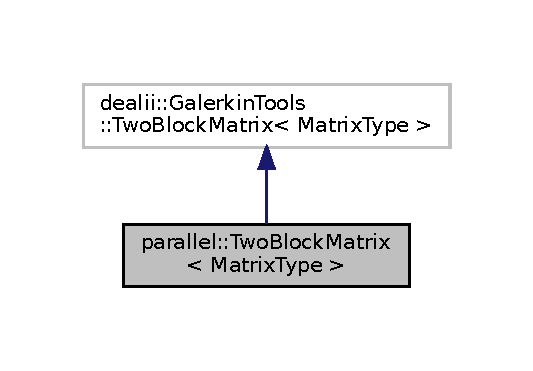
\includegraphics[width=240pt]{classparallel_1_1_two_block_matrix__inherit__graph}
\end{center}
\end{figure}


Collaboration diagram for parallel\+:\+:Two\+Block\+Matrix$<$ Matrix\+Type $>$\+:\nopagebreak
\begin{figure}[H]
\begin{center}
\leavevmode
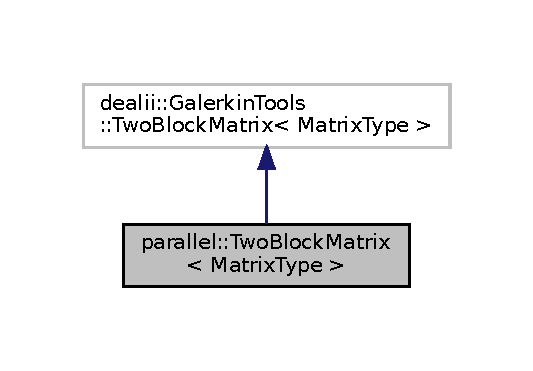
\includegraphics[width=240pt]{classparallel_1_1_two_block_matrix__coll__graph}
\end{center}
\end{figure}
\subsection*{Public Member Functions}
\begin{DoxyCompactItemize}
\item 
\hyperlink{classparallel_1_1_two_block_matrix_a93990616301e671f9a967fbc49029674}{Two\+Block\+Matrix} ()=default
\item 
\hyperlink{classparallel_1_1_two_block_matrix_afa9b3f1c3d74a211c334c8f6e59b52f6}{Two\+Block\+Matrix} (const \hyperlink{class_two_block_sparsity_pattern}{Two\+Block\+Sparsity\+Pattern} \&sp, const {\bf Index\+Set} \&locally\+\_\+owned\+\_\+indices, const M\+P\+I\+\_\+\+Comm mpi\+\_\+communicator=M\+P\+I\+\_\+\+C\+O\+M\+M\+\_\+\+W\+O\+R\+LD)
\item 
void \hyperlink{classparallel_1_1_two_block_matrix_a0e112695034c69aa8a430efd9e7c37ef}{reinit} (const \hyperlink{class_two_block_sparsity_pattern}{Two\+Block\+Sparsity\+Pattern} \&sp, const {\bf Index\+Set} \&locally\+\_\+owned\+\_\+indices, const M\+P\+I\+\_\+\+Comm mpi\+\_\+communicator=M\+P\+I\+\_\+\+C\+O\+M\+M\+\_\+\+W\+O\+R\+LD)
\item 
dealii\+::\+Galerkin\+Tools\+::parallel\+::\+Two\+Block\+Matrix$<$ Matrix\+Type $>$ \& \hyperlink{classparallel_1_1_two_block_matrix_a8e2ba56ebc9ee5ad1fe7b1d8604e9669}{operator=} (const double {\bf value})
\item 
const M\+P\+I\+\_\+\+Comm \& \hyperlink{classparallel_1_1_two_block_matrix_a4894068aad11986f43c1221cd696dc2a}{get\+\_\+communicator} () const 
\end{DoxyCompactItemize}


\subsection{Detailed Description}
\subsubsection*{template$<$class Matrix\+Type$>$\\*
class parallel\+::\+Two\+Block\+Matrix$<$ Matrix\+Type $>$}

The parallel version of \hyperlink{class_two_block_matrix}{Two\+Block\+Matrix}


\begin{DoxyTemplParams}{Template Parameters}
{\em Matrix\+Type} & The internal type of the matrix blocks \\
\hline
\end{DoxyTemplParams}


\subsection{Constructor \& Destructor Documentation}
\index{parallel\+::\+Two\+Block\+Matrix@{parallel\+::\+Two\+Block\+Matrix}!Two\+Block\+Matrix@{Two\+Block\+Matrix}}
\index{Two\+Block\+Matrix@{Two\+Block\+Matrix}!parallel\+::\+Two\+Block\+Matrix@{parallel\+::\+Two\+Block\+Matrix}}
\subsubsection[{\texorpdfstring{Two\+Block\+Matrix()=default}{TwoBlockMatrix()=default}}]{\setlength{\rightskip}{0pt plus 5cm}template$<$class Matrix\+Type$>$ {\bf parallel\+::\+Two\+Block\+Matrix}$<$ Matrix\+Type $>$\+::{\bf Two\+Block\+Matrix} (
\begin{DoxyParamCaption}
{}
\end{DoxyParamCaption}
)\hspace{0.3cm}{\ttfamily [default]}}\hypertarget{classparallel_1_1_two_block_matrix_a93990616301e671f9a967fbc49029674}{}\label{classparallel_1_1_two_block_matrix_a93990616301e671f9a967fbc49029674}
\index{parallel\+::\+Two\+Block\+Matrix@{parallel\+::\+Two\+Block\+Matrix}!Two\+Block\+Matrix@{Two\+Block\+Matrix}}
\index{Two\+Block\+Matrix@{Two\+Block\+Matrix}!parallel\+::\+Two\+Block\+Matrix@{parallel\+::\+Two\+Block\+Matrix}}
\subsubsection[{\texorpdfstring{Two\+Block\+Matrix(const Two\+Block\+Sparsity\+Pattern \&sp, const Index\+Set \&locally\+\_\+owned\+\_\+indices, const M\+P\+I\+\_\+\+Comm mpi\+\_\+communicator=\+M\+P\+I\+\_\+\+C\+O\+M\+M\+\_\+\+W\+O\+R\+L\+D)}{TwoBlockMatrix(const TwoBlockSparsityPattern &sp, const IndexSet &locally_owned_indices, const MPI_Comm mpi_communicator=MPI_COMM_WORLD)}}]{\setlength{\rightskip}{0pt plus 5cm}template$<$class Matrix\+Type$>$ {\bf parallel\+::\+Two\+Block\+Matrix}$<$ Matrix\+Type $>$\+::{\bf Two\+Block\+Matrix} (
\begin{DoxyParamCaption}
\item[{const {\bf Two\+Block\+Sparsity\+Pattern} \&}]{sp, }
\item[{const {\bf Index\+Set} \&}]{locally\+\_\+owned\+\_\+indices, }
\item[{const M\+P\+I\+\_\+\+Comm}]{mpi\+\_\+communicator = {\ttfamily MPI\+\_\+COMM\+\_\+WORLD}}
\end{DoxyParamCaption}
)}\hypertarget{classparallel_1_1_two_block_matrix_afa9b3f1c3d74a211c334c8f6e59b52f6}{}\label{classparallel_1_1_two_block_matrix_afa9b3f1c3d74a211c334c8f6e59b52f6}
Constructor for the parallel case


\begin{DoxyParams}[1]{Parameters}
\mbox{\tt in}  & {\em sp} & The sparsity pattern for the matrix\\
\hline
\mbox{\tt in}  & {\em locally\+\_\+owned\+\_\+indices} & The locally owned rows of \hyperlink{class_two_block_matrix_a91b02f00cf56b398e1624227e6efc8c6}{Two\+Block\+Matrix\+::A}\\
\hline
\mbox{\tt in}  & {\em mpi\+\_\+communicator} & The M\+PI communicator to be used \\
\hline
\end{DoxyParams}


\subsection{Member Function Documentation}
\index{parallel\+::\+Two\+Block\+Matrix@{parallel\+::\+Two\+Block\+Matrix}!get\+\_\+communicator@{get\+\_\+communicator}}
\index{get\+\_\+communicator@{get\+\_\+communicator}!parallel\+::\+Two\+Block\+Matrix@{parallel\+::\+Two\+Block\+Matrix}}
\subsubsection[{\texorpdfstring{get\+\_\+communicator() const }{get_communicator() const }}]{\setlength{\rightskip}{0pt plus 5cm}template$<$class Matrix\+Type$>$ const M\+P\+I\+\_\+\+Comm\& {\bf parallel\+::\+Two\+Block\+Matrix}$<$ Matrix\+Type $>$\+::get\+\_\+communicator (
\begin{DoxyParamCaption}
{}
\end{DoxyParamCaption}
) const}\hypertarget{classparallel_1_1_two_block_matrix_a4894068aad11986f43c1221cd696dc2a}{}\label{classparallel_1_1_two_block_matrix_a4894068aad11986f43c1221cd696dc2a}
\begin{DoxyReturn}{Returns}
The mpi communicator 
\end{DoxyReturn}
\index{parallel\+::\+Two\+Block\+Matrix@{parallel\+::\+Two\+Block\+Matrix}!operator=@{operator=}}
\index{operator=@{operator=}!parallel\+::\+Two\+Block\+Matrix@{parallel\+::\+Two\+Block\+Matrix}}
\subsubsection[{\texorpdfstring{operator=(const double value)}{operator=(const double value)}}]{\setlength{\rightskip}{0pt plus 5cm}template$<$class Matrix\+Type$>$ dealii\+::\+Galerkin\+Tools\+::parallel\+::\+Two\+Block\+Matrix$<$Matrix\+Type$>$\& {\bf parallel\+::\+Two\+Block\+Matrix}$<$ Matrix\+Type $>$\+::operator= (
\begin{DoxyParamCaption}
\item[{const double}]{value}
\end{DoxyParamCaption}
)}\hypertarget{classparallel_1_1_two_block_matrix_a8e2ba56ebc9ee5ad1fe7b1d8604e9669}{}\label{classparallel_1_1_two_block_matrix_a8e2ba56ebc9ee5ad1fe7b1d8604e9669}
Function setting all elements of the matrix to {\ttfamily value} 


\begin{DoxyParams}[1]{Parameters}
\mbox{\tt in}  & {\em value} & Only 0 is allowed for the value. \\
\hline
\end{DoxyParams}
\index{parallel\+::\+Two\+Block\+Matrix@{parallel\+::\+Two\+Block\+Matrix}!reinit@{reinit}}
\index{reinit@{reinit}!parallel\+::\+Two\+Block\+Matrix@{parallel\+::\+Two\+Block\+Matrix}}
\subsubsection[{\texorpdfstring{reinit(const Two\+Block\+Sparsity\+Pattern \&sp, const Index\+Set \&locally\+\_\+owned\+\_\+indices, const M\+P\+I\+\_\+\+Comm mpi\+\_\+communicator=\+M\+P\+I\+\_\+\+C\+O\+M\+M\+\_\+\+W\+O\+R\+L\+D)}{reinit(const TwoBlockSparsityPattern &sp, const IndexSet &locally_owned_indices, const MPI_Comm mpi_communicator=MPI_COMM_WORLD)}}]{\setlength{\rightskip}{0pt plus 5cm}template$<$class Matrix\+Type$>$ void {\bf parallel\+::\+Two\+Block\+Matrix}$<$ Matrix\+Type $>$\+::reinit (
\begin{DoxyParamCaption}
\item[{const {\bf Two\+Block\+Sparsity\+Pattern} \&}]{sp, }
\item[{const {\bf Index\+Set} \&}]{locally\+\_\+owned\+\_\+indices, }
\item[{const M\+P\+I\+\_\+\+Comm}]{mpi\+\_\+communicator = {\ttfamily MPI\+\_\+COMM\+\_\+WORLD}}
\end{DoxyParamCaption}
)}\hypertarget{classparallel_1_1_two_block_matrix_a0e112695034c69aa8a430efd9e7c37ef}{}\label{classparallel_1_1_two_block_matrix_a0e112695034c69aa8a430efd9e7c37ef}
Reinitialize the object


\begin{DoxyParams}[1]{Parameters}
\mbox{\tt in}  & {\em sp} & The sparsity pattern for the matrix\\
\hline
\mbox{\tt in}  & {\em locally\+\_\+owned\+\_\+indices} & The locally owned rows of \hyperlink{class_two_block_matrix_a91b02f00cf56b398e1624227e6efc8c6}{Two\+Block\+Matrix\+::A}\\
\hline
\mbox{\tt in}  & {\em mpi\+\_\+communicator} & The M\+PI communicator to be used \\
\hline
\end{DoxyParams}


The documentation for this class was generated from the following file\+:\begin{DoxyCompactItemize}
\item 
/home/sst/code/\+Galerkin\+Tools/\+Galerkin\+Tools/include/galerkin\+\_\+tools/\hyperlink{two__block__matrix_8h}{two\+\_\+block\+\_\+matrix.\+h}\end{DoxyCompactItemize}

\hypertarget{class_two_block_matrix}{}\section{Two\+Block\+Matrix$<$ Matrix\+Type $>$ Class Template Reference}
\label{class_two_block_matrix}\index{Two\+Block\+Matrix$<$ Matrix\+Type $>$@{Two\+Block\+Matrix$<$ Matrix\+Type $>$}}


{\ttfamily \#include $<$two\+\_\+block\+\_\+matrix.\+h$>$}



Collaboration diagram for Two\+Block\+Matrix$<$ Matrix\+Type $>$\+:\nopagebreak
\begin{figure}[H]
\begin{center}
\leavevmode
\includegraphics[width=261pt]{class_two_block_matrix__coll__graph}
\end{center}
\end{figure}
\subsection*{Public Types}
\begin{DoxyCompactItemize}
\item 
using \hyperlink{class_two_block_matrix_a9f50fb1f98df3ae0048c3c5220aa265f}{value\+\_\+type} = double
\end{DoxyCompactItemize}
\subsection*{Public Member Functions}
\begin{DoxyCompactItemize}
\item 
\hyperlink{class_two_block_matrix_aa74bb5722415e61241b5f38c9df29d39}{Two\+Block\+Matrix} ()=default
\item 
\hyperlink{class_two_block_matrix_a861cdc13c0fc6a65ec7d99e4d2349a92}{Two\+Block\+Matrix} (const \hyperlink{class_two_block_sparsity_pattern}{Two\+Block\+Sparsity\+Pattern} \&sp)
\item 
virtual \hyperlink{class_two_block_matrix_a0674b188ebc7bde3ee8f5eb9a94d6265}{$\sim$\+Two\+Block\+Matrix} ()=default
\item 
void \hyperlink{class_two_block_matrix_a5eaa76e9909c600aaa256aa77b577391}{reinit} (const \hyperlink{class_two_block_sparsity_pattern}{Two\+Block\+Sparsity\+Pattern} \&sp)
\item 
unsigned int \hyperlink{class_two_block_matrix_ab15732600f7e6917f961dce5e24b61a6}{m} () const 
\item 
unsigned int \hyperlink{class_two_block_matrix_a7675abf4c2532f48eb3b6bf153755a26}{n} () const 
\item 
void \hyperlink{class_two_block_matrix_a9b5d922689d1f60cbc59d2e424df2dc4}{add} (const unsigned int i, const unsigned int j, const double {\bf value})
\item 
void \hyperlink{class_two_block_matrix_a7373229281e1c3712681c1ac742dffb7}{add} (const unsigned int row, const unsigned int n\+\_\+cols, const unsigned int $\ast$col\+\_\+indices, const double $\ast${\bf values}, const bool elide\+\_\+zero\+\_\+values=false, const bool col\+\_\+indices\+\_\+are\+\_\+sorted=false)
\item 
void \hyperlink{class_two_block_matrix_a5457fd3b6228bed7a731bab2569a17a0}{set} (const unsigned int i, const unsigned int j, const double {\bf value})
\item 
double \hyperlink{class_two_block_matrix_a618495b0ad4cef72d95db7a1f380c20f}{operator()} (const unsigned int i, const unsigned int j) const 
\item 
double \hyperlink{class_two_block_matrix_a67a13d33b3110985bfc604969fc454c9}{el} (const unsigned int i, const unsigned int j) const 
\item 
\hyperlink{class_two_block_matrix}{Two\+Block\+Matrix}$<$ Matrix\+Type $>$ \& \hyperlink{class_two_block_matrix_ac008679a935fb6577931058ac0a6be36}{operator=} (const double {\bf value})
\item 
void \hyperlink{class_two_block_matrix_a8de26ebbb410811059d162fb164cedce}{compress} (const {\bf Vector\+Operation\+::values} operation)
\item 
const Matrix\+Type \& \hyperlink{class_two_block_matrix_a304eac57c72f23cbcf18a04e5bc64508}{get\+\_\+A} () const 
\item 
const Matrix\+Type \& \hyperlink{class_two_block_matrix_ab3807e975c3a5de9779a80c8d61fad96}{get\+\_\+B} () const 
\item 
const Matrix\+Type \& \hyperlink{class_two_block_matrix_ac0b0e0bc16412dfd73a8c6a3f782b8d9}{get\+\_\+C} () const 
\item 
const Matrix\+Type \& \hyperlink{class_two_block_matrix_af905a0e4b0504e45937a06df768a2ae2}{get\+\_\+D} () const 
\item 
Matrix\+Type \& \hyperlink{class_two_block_matrix_ab30f0e3b8f803456c3a2f1ce4f753081}{get\+\_\+A} ()
\item 
Matrix\+Type \& \hyperlink{class_two_block_matrix_ae41ca5bbc0495c8ffb1604da488a33b7}{get\+\_\+B} ()
\item 
Matrix\+Type \& \hyperlink{class_two_block_matrix_aeaa4102bb137700d7bbe0262ee16e8ee}{get\+\_\+C} ()
\item 
Matrix\+Type \& \hyperlink{class_two_block_matrix_a3725800849e26e2192c0ac6520777dab}{get\+\_\+D} ()
\item 
unsigned int \hyperlink{class_two_block_matrix_a688b1a69284ec154c493a99ec7cad704}{get\+\_\+block\+\_\+0\+\_\+size} () const 
\item 
unsigned int \hyperlink{class_two_block_matrix_a9ecb16be5aa5ebbb916d256a9ded7c3e}{get\+\_\+block\+\_\+1\+\_\+size} () const 
\end{DoxyCompactItemize}
\subsection*{Protected Attributes}
\begin{DoxyCompactItemize}
\item 
Matrix\+Type \hyperlink{class_two_block_matrix_a91b02f00cf56b398e1624227e6efc8c6}{A}
\item 
Matrix\+Type \hyperlink{class_two_block_matrix_ae8edfe1cd2298741586dcc46a4d09ebf}{B}
\item 
Matrix\+Type \hyperlink{class_two_block_matrix_a847505a77448124928540be0367d8747}{C}
\item 
Matrix\+Type \hyperlink{class_two_block_matrix_a72c598f36d3e8cce12821a09920ded2d}{D}
\item 
{\bf Sparsity\+Pattern} \hyperlink{class_two_block_matrix_af40216911c197c73687f7d3a1ff4e68e}{sp\+\_\+A}
\item 
{\bf Sparsity\+Pattern} \hyperlink{class_two_block_matrix_a854c7e77623a7c0012aa0ceeb60c147a}{sp\+\_\+B}
\item 
{\bf Sparsity\+Pattern} \hyperlink{class_two_block_matrix_a45d6e534ad775577c86e9ac9a116014e}{sp\+\_\+C}
\item 
{\bf Sparsity\+Pattern} \hyperlink{class_two_block_matrix_adb1833352096be79279134b218659665}{sp\+\_\+D}
\item 
unsigned int \hyperlink{class_two_block_matrix_ae862db333ed43f1650d4926f237cfc43}{block\+\_\+0\+\_\+size} = 0
\item 
unsigned int \hyperlink{class_two_block_matrix_a60ddea1d26313aac35cfb2ae9f192cb2}{block\+\_\+1\+\_\+size} = 0
\item 
unsigned int \hyperlink{class_two_block_matrix_a7d63b4c4c1e499c9f9913444dc5fd6b6}{total\+\_\+dimension} = 0
\end{DoxyCompactItemize}


\subsection{Detailed Description}
\subsubsection*{template$<$class Matrix\+Type$>$\\*
class Two\+Block\+Matrix$<$ Matrix\+Type $>$}

This class implements a block matrix of the form \begin{equation*} \begin{pmatrix} \boldsymbol{A} & \boldsymbol{B} \\ \boldsymbol{C}^\top & \boldsymbol{D} \end{pmatrix} \end{equation*}

The main difference to the deal.\+II block matrices is that internally $\boldsymbol{C}$ is stored instead of the transpose of it. This is useful for parallel applications where finite element related dofs are coupled to \char`\"{}global\char`\"{} unknowns which are not related to any mesh.


\begin{DoxyTemplParams}{Template Parameters}
{\em Matrix\+Type} & The internal type of the matrix blocks \\
\hline
\end{DoxyTemplParams}


\subsection{Member Typedef Documentation}
\index{Two\+Block\+Matrix@{Two\+Block\+Matrix}!value\+\_\+type@{value\+\_\+type}}
\index{value\+\_\+type@{value\+\_\+type}!Two\+Block\+Matrix@{Two\+Block\+Matrix}}
\subsubsection[{\texorpdfstring{value\+\_\+type}{value_type}}]{\setlength{\rightskip}{0pt plus 5cm}template$<$class Matrix\+Type$>$ using {\bf Two\+Block\+Matrix}$<$ Matrix\+Type $>$\+::{\bf value\+\_\+type} =  double}\hypertarget{class_two_block_matrix_a9f50fb1f98df3ae0048c3c5220aa265f}{}\label{class_two_block_matrix_a9f50fb1f98df3ae0048c3c5220aa265f}


\subsection{Constructor \& Destructor Documentation}
\index{Two\+Block\+Matrix@{Two\+Block\+Matrix}!Two\+Block\+Matrix@{Two\+Block\+Matrix}}
\index{Two\+Block\+Matrix@{Two\+Block\+Matrix}!Two\+Block\+Matrix@{Two\+Block\+Matrix}}
\subsubsection[{\texorpdfstring{Two\+Block\+Matrix()=default}{TwoBlockMatrix()=default}}]{\setlength{\rightskip}{0pt plus 5cm}template$<$class Matrix\+Type$>$ {\bf Two\+Block\+Matrix}$<$ Matrix\+Type $>$\+::{\bf Two\+Block\+Matrix} (
\begin{DoxyParamCaption}
{}
\end{DoxyParamCaption}
)\hspace{0.3cm}{\ttfamily [default]}}\hypertarget{class_two_block_matrix_aa74bb5722415e61241b5f38c9df29d39}{}\label{class_two_block_matrix_aa74bb5722415e61241b5f38c9df29d39}
Default constructor \index{Two\+Block\+Matrix@{Two\+Block\+Matrix}!Two\+Block\+Matrix@{Two\+Block\+Matrix}}
\index{Two\+Block\+Matrix@{Two\+Block\+Matrix}!Two\+Block\+Matrix@{Two\+Block\+Matrix}}
\subsubsection[{\texorpdfstring{Two\+Block\+Matrix(const Two\+Block\+Sparsity\+Pattern \&sp)}{TwoBlockMatrix(const TwoBlockSparsityPattern &sp)}}]{\setlength{\rightskip}{0pt plus 5cm}template$<$class Matrix\+Type$>$ {\bf Two\+Block\+Matrix}$<$ Matrix\+Type $>$\+::{\bf Two\+Block\+Matrix} (
\begin{DoxyParamCaption}
\item[{const {\bf Two\+Block\+Sparsity\+Pattern} \&}]{sp}
\end{DoxyParamCaption}
)}\hypertarget{class_two_block_matrix_a861cdc13c0fc6a65ec7d99e4d2349a92}{}\label{class_two_block_matrix_a861cdc13c0fc6a65ec7d99e4d2349a92}
Constructor for the sequential case


\begin{DoxyParams}[1]{Parameters}
\mbox{\tt in}  & {\em sp} & The sparsity pattern for the matrix \\
\hline
\end{DoxyParams}
\index{Two\+Block\+Matrix@{Two\+Block\+Matrix}!````~Two\+Block\+Matrix@{$\sim$\+Two\+Block\+Matrix}}
\index{````~Two\+Block\+Matrix@{$\sim$\+Two\+Block\+Matrix}!Two\+Block\+Matrix@{Two\+Block\+Matrix}}
\subsubsection[{\texorpdfstring{$\sim$\+Two\+Block\+Matrix()=default}{~TwoBlockMatrix()=default}}]{\setlength{\rightskip}{0pt plus 5cm}template$<$class Matrix\+Type$>$ virtual {\bf Two\+Block\+Matrix}$<$ Matrix\+Type $>$\+::$\sim${\bf Two\+Block\+Matrix} (
\begin{DoxyParamCaption}
{}
\end{DoxyParamCaption}
)\hspace{0.3cm}{\ttfamily [virtual]}, {\ttfamily [default]}}\hypertarget{class_two_block_matrix_a0674b188ebc7bde3ee8f5eb9a94d6265}{}\label{class_two_block_matrix_a0674b188ebc7bde3ee8f5eb9a94d6265}
Virtual destructor to make the class polymorphic and allow dynamic casts. 

\subsection{Member Function Documentation}
\index{Two\+Block\+Matrix@{Two\+Block\+Matrix}!add@{add}}
\index{add@{add}!Two\+Block\+Matrix@{Two\+Block\+Matrix}}
\subsubsection[{\texorpdfstring{add(const unsigned int i, const unsigned int j, const double value)}{add(const unsigned int i, const unsigned int j, const double value)}}]{\setlength{\rightskip}{0pt plus 5cm}template$<$class Matrix\+Type$>$ void {\bf Two\+Block\+Matrix}$<$ Matrix\+Type $>$\+::add (
\begin{DoxyParamCaption}
\item[{const unsigned int}]{i, }
\item[{const unsigned int}]{j, }
\item[{const double}]{value}
\end{DoxyParamCaption}
)}\hypertarget{class_two_block_matrix_a9b5d922689d1f60cbc59d2e424df2dc4}{}\label{class_two_block_matrix_a9b5d922689d1f60cbc59d2e424df2dc4}
Function adding to an element of the matrix


\begin{DoxyParams}[1]{Parameters}
\mbox{\tt in}  & {\em i} & row\\
\hline
\mbox{\tt in}  & {\em j} & column\\
\hline
\mbox{\tt in}  & {\em value} & the number to be added \\
\hline
\end{DoxyParams}
\index{Two\+Block\+Matrix@{Two\+Block\+Matrix}!add@{add}}
\index{add@{add}!Two\+Block\+Matrix@{Two\+Block\+Matrix}}
\subsubsection[{\texorpdfstring{add(const unsigned int row, const unsigned int n\+\_\+cols, const unsigned int $\ast$col\+\_\+indices, const double $\ast$values, const bool elide\+\_\+zero\+\_\+values=false, const bool col\+\_\+indices\+\_\+are\+\_\+sorted=false)}{add(const unsigned int row, const unsigned int n_cols, const unsigned int *col_indices, const double *values, const bool elide_zero_values=false, const bool col_indices_are_sorted=false)}}]{\setlength{\rightskip}{0pt plus 5cm}template$<$class Matrix\+Type$>$ void {\bf Two\+Block\+Matrix}$<$ Matrix\+Type $>$\+::add (
\begin{DoxyParamCaption}
\item[{const unsigned int}]{row, }
\item[{const unsigned int}]{n\+\_\+cols, }
\item[{const unsigned int $\ast$}]{col\+\_\+indices, }
\item[{const double $\ast$}]{values, }
\item[{const bool}]{elide\+\_\+zero\+\_\+values = {\ttfamily false}, }
\item[{const bool}]{col\+\_\+indices\+\_\+are\+\_\+sorted = {\ttfamily false}}
\end{DoxyParamCaption}
)}\hypertarget{class_two_block_matrix_a7373229281e1c3712681c1ac742dffb7}{}\label{class_two_block_matrix_a7373229281e1c3712681c1ac742dffb7}
Add an array of values given by {\ttfamily values} in the given global matrix row at columns specified by {\ttfamily col\+\_\+indices} in the sparse matrix.


\begin{DoxyParams}[1]{Parameters}
\mbox{\tt in}  & {\em row} & The row to add to\\
\hline
\mbox{\tt in}  & {\em n\+\_\+cols} & The number of values\\
\hline
\mbox{\tt in}  & {\em col\+\_\+indices} & The column indices\\
\hline
\mbox{\tt in}  & {\em values} & The values\\
\hline
\mbox{\tt in}  & {\em elide\+\_\+zero\+\_\+values} & This only exists for compatibility with deal.\+II and does not affect what\textquotesingle{}s going on in this function\\
\hline
\mbox{\tt in}  & {\em col\+\_\+indices\+\_\+are\+\_\+sorted} & This only exists for compatibility with deal.\+II and does not affect what\textquotesingle{}s going on in this function \\
\hline
\end{DoxyParams}
\index{Two\+Block\+Matrix@{Two\+Block\+Matrix}!compress@{compress}}
\index{compress@{compress}!Two\+Block\+Matrix@{Two\+Block\+Matrix}}
\subsubsection[{\texorpdfstring{compress(const Vector\+Operation\+::values operation)}{compress(const VectorOperation::values operation)}}]{\setlength{\rightskip}{0pt plus 5cm}template$<$class Matrix\+Type$>$ void {\bf Two\+Block\+Matrix}$<$ Matrix\+Type $>$\+::compress (
\begin{DoxyParamCaption}
\item[{const {\bf Vector\+Operation\+::values}}]{operation}
\end{DoxyParamCaption}
)}\hypertarget{class_two_block_matrix_a8de26ebbb410811059d162fb164cedce}{}\label{class_two_block_matrix_a8de26ebbb410811059d162fb164cedce}
Function compressing this matrix


\begin{DoxyParams}[1]{Parameters}
\mbox{\tt in}  & {\em operation} & The operation (typically add or insert) \\
\hline
\end{DoxyParams}
\index{Two\+Block\+Matrix@{Two\+Block\+Matrix}!el@{el}}
\index{el@{el}!Two\+Block\+Matrix@{Two\+Block\+Matrix}}
\subsubsection[{\texorpdfstring{el(const unsigned int i, const unsigned int j) const }{el(const unsigned int i, const unsigned int j) const }}]{\setlength{\rightskip}{0pt plus 5cm}template$<$class Matrix\+Type$>$ double {\bf Two\+Block\+Matrix}$<$ Matrix\+Type $>$\+::el (
\begin{DoxyParamCaption}
\item[{const unsigned int}]{i, }
\item[{const unsigned int}]{j}
\end{DoxyParamCaption}
) const}\hypertarget{class_two_block_matrix_a67a13d33b3110985bfc604969fc454c9}{}\label{class_two_block_matrix_a67a13d33b3110985bfc604969fc454c9}
Return an element of the matrix (if the entry does not exist in the sparsity pattern, 0 is returned) \index{Two\+Block\+Matrix@{Two\+Block\+Matrix}!get\+\_\+A@{get\+\_\+A}}
\index{get\+\_\+A@{get\+\_\+A}!Two\+Block\+Matrix@{Two\+Block\+Matrix}}
\subsubsection[{\texorpdfstring{get\+\_\+\+A() const }{get_A() const }}]{\setlength{\rightskip}{0pt plus 5cm}template$<$class Matrix\+Type$>$ const Matrix\+Type\& {\bf Two\+Block\+Matrix}$<$ Matrix\+Type $>$\+::get\+\_\+A (
\begin{DoxyParamCaption}
{}
\end{DoxyParamCaption}
) const}\hypertarget{class_two_block_matrix_a304eac57c72f23cbcf18a04e5bc64508}{}\label{class_two_block_matrix_a304eac57c72f23cbcf18a04e5bc64508}
\begin{DoxyReturn}{Returns}
const reference to A 
\end{DoxyReturn}
\index{Two\+Block\+Matrix@{Two\+Block\+Matrix}!get\+\_\+A@{get\+\_\+A}}
\index{get\+\_\+A@{get\+\_\+A}!Two\+Block\+Matrix@{Two\+Block\+Matrix}}
\subsubsection[{\texorpdfstring{get\+\_\+\+A()}{get_A()}}]{\setlength{\rightskip}{0pt plus 5cm}template$<$class Matrix\+Type$>$ Matrix\+Type\& {\bf Two\+Block\+Matrix}$<$ Matrix\+Type $>$\+::get\+\_\+A (
\begin{DoxyParamCaption}
{}
\end{DoxyParamCaption}
)}\hypertarget{class_two_block_matrix_ab30f0e3b8f803456c3a2f1ce4f753081}{}\label{class_two_block_matrix_ab30f0e3b8f803456c3a2f1ce4f753081}
\begin{DoxyReturn}{Returns}
reference to A 
\end{DoxyReturn}
\index{Two\+Block\+Matrix@{Two\+Block\+Matrix}!get\+\_\+B@{get\+\_\+B}}
\index{get\+\_\+B@{get\+\_\+B}!Two\+Block\+Matrix@{Two\+Block\+Matrix}}
\subsubsection[{\texorpdfstring{get\+\_\+\+B() const }{get_B() const }}]{\setlength{\rightskip}{0pt plus 5cm}template$<$class Matrix\+Type$>$ const Matrix\+Type\& {\bf Two\+Block\+Matrix}$<$ Matrix\+Type $>$\+::get\+\_\+B (
\begin{DoxyParamCaption}
{}
\end{DoxyParamCaption}
) const}\hypertarget{class_two_block_matrix_ab3807e975c3a5de9779a80c8d61fad96}{}\label{class_two_block_matrix_ab3807e975c3a5de9779a80c8d61fad96}
\begin{DoxyReturn}{Returns}
const reference to B 
\end{DoxyReturn}
\index{Two\+Block\+Matrix@{Two\+Block\+Matrix}!get\+\_\+B@{get\+\_\+B}}
\index{get\+\_\+B@{get\+\_\+B}!Two\+Block\+Matrix@{Two\+Block\+Matrix}}
\subsubsection[{\texorpdfstring{get\+\_\+\+B()}{get_B()}}]{\setlength{\rightskip}{0pt plus 5cm}template$<$class Matrix\+Type$>$ Matrix\+Type\& {\bf Two\+Block\+Matrix}$<$ Matrix\+Type $>$\+::get\+\_\+B (
\begin{DoxyParamCaption}
{}
\end{DoxyParamCaption}
)}\hypertarget{class_two_block_matrix_ae41ca5bbc0495c8ffb1604da488a33b7}{}\label{class_two_block_matrix_ae41ca5bbc0495c8ffb1604da488a33b7}
\begin{DoxyReturn}{Returns}
reference to B 
\end{DoxyReturn}
\index{Two\+Block\+Matrix@{Two\+Block\+Matrix}!get\+\_\+block\+\_\+0\+\_\+size@{get\+\_\+block\+\_\+0\+\_\+size}}
\index{get\+\_\+block\+\_\+0\+\_\+size@{get\+\_\+block\+\_\+0\+\_\+size}!Two\+Block\+Matrix@{Two\+Block\+Matrix}}
\subsubsection[{\texorpdfstring{get\+\_\+block\+\_\+0\+\_\+size() const }{get_block_0_size() const }}]{\setlength{\rightskip}{0pt plus 5cm}template$<$class Matrix\+Type$>$ unsigned int {\bf Two\+Block\+Matrix}$<$ Matrix\+Type $>$\+::get\+\_\+block\+\_\+0\+\_\+size (
\begin{DoxyParamCaption}
{}
\end{DoxyParamCaption}
) const}\hypertarget{class_two_block_matrix_a688b1a69284ec154c493a99ec7cad704}{}\label{class_two_block_matrix_a688b1a69284ec154c493a99ec7cad704}
\begin{DoxyReturn}{Returns}
\hyperlink{class_two_block_matrix_ae862db333ed43f1650d4926f237cfc43}{Two\+Block\+Matrix\+::block\+\_\+0\+\_\+size} 
\end{DoxyReturn}
\index{Two\+Block\+Matrix@{Two\+Block\+Matrix}!get\+\_\+block\+\_\+1\+\_\+size@{get\+\_\+block\+\_\+1\+\_\+size}}
\index{get\+\_\+block\+\_\+1\+\_\+size@{get\+\_\+block\+\_\+1\+\_\+size}!Two\+Block\+Matrix@{Two\+Block\+Matrix}}
\subsubsection[{\texorpdfstring{get\+\_\+block\+\_\+1\+\_\+size() const }{get_block_1_size() const }}]{\setlength{\rightskip}{0pt plus 5cm}template$<$class Matrix\+Type$>$ unsigned int {\bf Two\+Block\+Matrix}$<$ Matrix\+Type $>$\+::get\+\_\+block\+\_\+1\+\_\+size (
\begin{DoxyParamCaption}
{}
\end{DoxyParamCaption}
) const}\hypertarget{class_two_block_matrix_a9ecb16be5aa5ebbb916d256a9ded7c3e}{}\label{class_two_block_matrix_a9ecb16be5aa5ebbb916d256a9ded7c3e}
\begin{DoxyReturn}{Returns}
\hyperlink{class_two_block_matrix_a60ddea1d26313aac35cfb2ae9f192cb2}{Two\+Block\+Matrix\+::block\+\_\+1\+\_\+size} 
\end{DoxyReturn}
\index{Two\+Block\+Matrix@{Two\+Block\+Matrix}!get\+\_\+C@{get\+\_\+C}}
\index{get\+\_\+C@{get\+\_\+C}!Two\+Block\+Matrix@{Two\+Block\+Matrix}}
\subsubsection[{\texorpdfstring{get\+\_\+\+C() const }{get_C() const }}]{\setlength{\rightskip}{0pt plus 5cm}template$<$class Matrix\+Type$>$ const Matrix\+Type\& {\bf Two\+Block\+Matrix}$<$ Matrix\+Type $>$\+::get\+\_\+C (
\begin{DoxyParamCaption}
{}
\end{DoxyParamCaption}
) const}\hypertarget{class_two_block_matrix_ac0b0e0bc16412dfd73a8c6a3f782b8d9}{}\label{class_two_block_matrix_ac0b0e0bc16412dfd73a8c6a3f782b8d9}
\begin{DoxyReturn}{Returns}
const reference to C 
\end{DoxyReturn}
\index{Two\+Block\+Matrix@{Two\+Block\+Matrix}!get\+\_\+C@{get\+\_\+C}}
\index{get\+\_\+C@{get\+\_\+C}!Two\+Block\+Matrix@{Two\+Block\+Matrix}}
\subsubsection[{\texorpdfstring{get\+\_\+\+C()}{get_C()}}]{\setlength{\rightskip}{0pt plus 5cm}template$<$class Matrix\+Type$>$ Matrix\+Type\& {\bf Two\+Block\+Matrix}$<$ Matrix\+Type $>$\+::get\+\_\+C (
\begin{DoxyParamCaption}
{}
\end{DoxyParamCaption}
)}\hypertarget{class_two_block_matrix_aeaa4102bb137700d7bbe0262ee16e8ee}{}\label{class_two_block_matrix_aeaa4102bb137700d7bbe0262ee16e8ee}
\begin{DoxyReturn}{Returns}
reference to C 
\end{DoxyReturn}
\index{Two\+Block\+Matrix@{Two\+Block\+Matrix}!get\+\_\+D@{get\+\_\+D}}
\index{get\+\_\+D@{get\+\_\+D}!Two\+Block\+Matrix@{Two\+Block\+Matrix}}
\subsubsection[{\texorpdfstring{get\+\_\+\+D() const }{get_D() const }}]{\setlength{\rightskip}{0pt plus 5cm}template$<$class Matrix\+Type$>$ const Matrix\+Type\& {\bf Two\+Block\+Matrix}$<$ Matrix\+Type $>$\+::get\+\_\+D (
\begin{DoxyParamCaption}
{}
\end{DoxyParamCaption}
) const}\hypertarget{class_two_block_matrix_af905a0e4b0504e45937a06df768a2ae2}{}\label{class_two_block_matrix_af905a0e4b0504e45937a06df768a2ae2}
\begin{DoxyReturn}{Returns}
const reference to D 
\end{DoxyReturn}
\index{Two\+Block\+Matrix@{Two\+Block\+Matrix}!get\+\_\+D@{get\+\_\+D}}
\index{get\+\_\+D@{get\+\_\+D}!Two\+Block\+Matrix@{Two\+Block\+Matrix}}
\subsubsection[{\texorpdfstring{get\+\_\+\+D()}{get_D()}}]{\setlength{\rightskip}{0pt plus 5cm}template$<$class Matrix\+Type$>$ Matrix\+Type\& {\bf Two\+Block\+Matrix}$<$ Matrix\+Type $>$\+::get\+\_\+D (
\begin{DoxyParamCaption}
{}
\end{DoxyParamCaption}
)}\hypertarget{class_two_block_matrix_a3725800849e26e2192c0ac6520777dab}{}\label{class_two_block_matrix_a3725800849e26e2192c0ac6520777dab}
\begin{DoxyReturn}{Returns}
reference to D 
\end{DoxyReturn}
\index{Two\+Block\+Matrix@{Two\+Block\+Matrix}!m@{m}}
\index{m@{m}!Two\+Block\+Matrix@{Two\+Block\+Matrix}}
\subsubsection[{\texorpdfstring{m() const }{m() const }}]{\setlength{\rightskip}{0pt plus 5cm}template$<$class Matrix\+Type$>$ unsigned int {\bf Two\+Block\+Matrix}$<$ Matrix\+Type $>$\+::m (
\begin{DoxyParamCaption}
{}
\end{DoxyParamCaption}
) const}\hypertarget{class_two_block_matrix_ab15732600f7e6917f961dce5e24b61a6}{}\label{class_two_block_matrix_ab15732600f7e6917f961dce5e24b61a6}
The total number of rows \index{Two\+Block\+Matrix@{Two\+Block\+Matrix}!n@{n}}
\index{n@{n}!Two\+Block\+Matrix@{Two\+Block\+Matrix}}
\subsubsection[{\texorpdfstring{n() const }{n() const }}]{\setlength{\rightskip}{0pt plus 5cm}template$<$class Matrix\+Type$>$ unsigned int {\bf Two\+Block\+Matrix}$<$ Matrix\+Type $>$\+::n (
\begin{DoxyParamCaption}
{}
\end{DoxyParamCaption}
) const}\hypertarget{class_two_block_matrix_a7675abf4c2532f48eb3b6bf153755a26}{}\label{class_two_block_matrix_a7675abf4c2532f48eb3b6bf153755a26}
The total number of columns \index{Two\+Block\+Matrix@{Two\+Block\+Matrix}!operator()@{operator()}}
\index{operator()@{operator()}!Two\+Block\+Matrix@{Two\+Block\+Matrix}}
\subsubsection[{\texorpdfstring{operator()(const unsigned int i, const unsigned int j) const }{operator()(const unsigned int i, const unsigned int j) const }}]{\setlength{\rightskip}{0pt plus 5cm}template$<$class Matrix\+Type$>$ double {\bf Two\+Block\+Matrix}$<$ Matrix\+Type $>$\+::operator() (
\begin{DoxyParamCaption}
\item[{const unsigned int}]{i, }
\item[{const unsigned int}]{j}
\end{DoxyParamCaption}
) const}\hypertarget{class_two_block_matrix_a618495b0ad4cef72d95db7a1f380c20f}{}\label{class_two_block_matrix_a618495b0ad4cef72d95db7a1f380c20f}
read access to element


\begin{DoxyParams}[1]{Parameters}
\mbox{\tt in}  & {\em i} & row\\
\hline
\mbox{\tt in}  & {\em j} & column \\
\hline
\end{DoxyParams}
\index{Two\+Block\+Matrix@{Two\+Block\+Matrix}!operator=@{operator=}}
\index{operator=@{operator=}!Two\+Block\+Matrix@{Two\+Block\+Matrix}}
\subsubsection[{\texorpdfstring{operator=(const double value)}{operator=(const double value)}}]{\setlength{\rightskip}{0pt plus 5cm}template$<$class Matrix\+Type$>$ {\bf Two\+Block\+Matrix}$<$Matrix\+Type$>$\& {\bf Two\+Block\+Matrix}$<$ Matrix\+Type $>$\+::operator= (
\begin{DoxyParamCaption}
\item[{const double}]{value}
\end{DoxyParamCaption}
)}\hypertarget{class_two_block_matrix_ac008679a935fb6577931058ac0a6be36}{}\label{class_two_block_matrix_ac008679a935fb6577931058ac0a6be36}
Function setting all elements of the matrix to {\ttfamily value} 


\begin{DoxyParams}[1]{Parameters}
\mbox{\tt in}  & {\em value} & Only 0 is allowed for the value. \\
\hline
\end{DoxyParams}
\index{Two\+Block\+Matrix@{Two\+Block\+Matrix}!reinit@{reinit}}
\index{reinit@{reinit}!Two\+Block\+Matrix@{Two\+Block\+Matrix}}
\subsubsection[{\texorpdfstring{reinit(const Two\+Block\+Sparsity\+Pattern \&sp)}{reinit(const TwoBlockSparsityPattern &sp)}}]{\setlength{\rightskip}{0pt plus 5cm}template$<$class Matrix\+Type$>$ void {\bf Two\+Block\+Matrix}$<$ Matrix\+Type $>$\+::reinit (
\begin{DoxyParamCaption}
\item[{const {\bf Two\+Block\+Sparsity\+Pattern} \&}]{sp}
\end{DoxyParamCaption}
)}\hypertarget{class_two_block_matrix_a5eaa76e9909c600aaa256aa77b577391}{}\label{class_two_block_matrix_a5eaa76e9909c600aaa256aa77b577391}
Reinitialize the object


\begin{DoxyParams}[1]{Parameters}
\mbox{\tt in}  & {\em sp} & The sparsity pattern for the matrix \\
\hline
\end{DoxyParams}
\index{Two\+Block\+Matrix@{Two\+Block\+Matrix}!set@{set}}
\index{set@{set}!Two\+Block\+Matrix@{Two\+Block\+Matrix}}
\subsubsection[{\texorpdfstring{set(const unsigned int i, const unsigned int j, const double value)}{set(const unsigned int i, const unsigned int j, const double value)}}]{\setlength{\rightskip}{0pt plus 5cm}template$<$class Matrix\+Type$>$ void {\bf Two\+Block\+Matrix}$<$ Matrix\+Type $>$\+::set (
\begin{DoxyParamCaption}
\item[{const unsigned int}]{i, }
\item[{const unsigned int}]{j, }
\item[{const double}]{value}
\end{DoxyParamCaption}
)}\hypertarget{class_two_block_matrix_a5457fd3b6228bed7a731bab2569a17a0}{}\label{class_two_block_matrix_a5457fd3b6228bed7a731bab2569a17a0}
Function setting an element of the matrix


\begin{DoxyParams}[1]{Parameters}
\mbox{\tt in}  & {\em i} & row\\
\hline
\mbox{\tt in}  & {\em j} & column\\
\hline
\mbox{\tt in}  & {\em value} & the number to be added \\
\hline
\end{DoxyParams}


\subsection{Member Data Documentation}
\index{Two\+Block\+Matrix@{Two\+Block\+Matrix}!A@{A}}
\index{A@{A}!Two\+Block\+Matrix@{Two\+Block\+Matrix}}
\subsubsection[{\texorpdfstring{A}{A}}]{\setlength{\rightskip}{0pt plus 5cm}template$<$class Matrix\+Type$>$ Matrix\+Type {\bf Two\+Block\+Matrix}$<$ Matrix\+Type $>$\+::A\hspace{0.3cm}{\ttfamily [protected]}}\hypertarget{class_two_block_matrix_a91b02f00cf56b398e1624227e6efc8c6}{}\label{class_two_block_matrix_a91b02f00cf56b398e1624227e6efc8c6}
The matrix A \index{Two\+Block\+Matrix@{Two\+Block\+Matrix}!B@{B}}
\index{B@{B}!Two\+Block\+Matrix@{Two\+Block\+Matrix}}
\subsubsection[{\texorpdfstring{B}{B}}]{\setlength{\rightskip}{0pt plus 5cm}template$<$class Matrix\+Type$>$ Matrix\+Type {\bf Two\+Block\+Matrix}$<$ Matrix\+Type $>$\+::B\hspace{0.3cm}{\ttfamily [protected]}}\hypertarget{class_two_block_matrix_ae8edfe1cd2298741586dcc46a4d09ebf}{}\label{class_two_block_matrix_ae8edfe1cd2298741586dcc46a4d09ebf}
The matrix B \index{Two\+Block\+Matrix@{Two\+Block\+Matrix}!block\+\_\+0\+\_\+size@{block\+\_\+0\+\_\+size}}
\index{block\+\_\+0\+\_\+size@{block\+\_\+0\+\_\+size}!Two\+Block\+Matrix@{Two\+Block\+Matrix}}
\subsubsection[{\texorpdfstring{block\+\_\+0\+\_\+size}{block_0_size}}]{\setlength{\rightskip}{0pt plus 5cm}template$<$class Matrix\+Type$>$ unsigned int {\bf Two\+Block\+Matrix}$<$ Matrix\+Type $>$\+::block\+\_\+0\+\_\+size = 0\hspace{0.3cm}{\ttfamily [protected]}}\hypertarget{class_two_block_matrix_ae862db333ed43f1650d4926f237cfc43}{}\label{class_two_block_matrix_ae862db333ed43f1650d4926f237cfc43}
The dimension of A \index{Two\+Block\+Matrix@{Two\+Block\+Matrix}!block\+\_\+1\+\_\+size@{block\+\_\+1\+\_\+size}}
\index{block\+\_\+1\+\_\+size@{block\+\_\+1\+\_\+size}!Two\+Block\+Matrix@{Two\+Block\+Matrix}}
\subsubsection[{\texorpdfstring{block\+\_\+1\+\_\+size}{block_1_size}}]{\setlength{\rightskip}{0pt plus 5cm}template$<$class Matrix\+Type$>$ unsigned int {\bf Two\+Block\+Matrix}$<$ Matrix\+Type $>$\+::block\+\_\+1\+\_\+size = 0\hspace{0.3cm}{\ttfamily [protected]}}\hypertarget{class_two_block_matrix_a60ddea1d26313aac35cfb2ae9f192cb2}{}\label{class_two_block_matrix_a60ddea1d26313aac35cfb2ae9f192cb2}
The dimension of D \index{Two\+Block\+Matrix@{Two\+Block\+Matrix}!C@{C}}
\index{C@{C}!Two\+Block\+Matrix@{Two\+Block\+Matrix}}
\subsubsection[{\texorpdfstring{C}{C}}]{\setlength{\rightskip}{0pt plus 5cm}template$<$class Matrix\+Type$>$ Matrix\+Type {\bf Two\+Block\+Matrix}$<$ Matrix\+Type $>$\+::C\hspace{0.3cm}{\ttfamily [protected]}}\hypertarget{class_two_block_matrix_a847505a77448124928540be0367d8747}{}\label{class_two_block_matrix_a847505a77448124928540be0367d8747}
The matrix C \index{Two\+Block\+Matrix@{Two\+Block\+Matrix}!D@{D}}
\index{D@{D}!Two\+Block\+Matrix@{Two\+Block\+Matrix}}
\subsubsection[{\texorpdfstring{D}{D}}]{\setlength{\rightskip}{0pt plus 5cm}template$<$class Matrix\+Type$>$ Matrix\+Type {\bf Two\+Block\+Matrix}$<$ Matrix\+Type $>$\+::D\hspace{0.3cm}{\ttfamily [protected]}}\hypertarget{class_two_block_matrix_a72c598f36d3e8cce12821a09920ded2d}{}\label{class_two_block_matrix_a72c598f36d3e8cce12821a09920ded2d}
The matrix D \index{Two\+Block\+Matrix@{Two\+Block\+Matrix}!sp\+\_\+A@{sp\+\_\+A}}
\index{sp\+\_\+A@{sp\+\_\+A}!Two\+Block\+Matrix@{Two\+Block\+Matrix}}
\subsubsection[{\texorpdfstring{sp\+\_\+A}{sp_A}}]{\setlength{\rightskip}{0pt plus 5cm}template$<$class Matrix\+Type$>$ {\bf Sparsity\+Pattern} {\bf Two\+Block\+Matrix}$<$ Matrix\+Type $>$\+::sp\+\_\+A\hspace{0.3cm}{\ttfamily [protected]}}\hypertarget{class_two_block_matrix_af40216911c197c73687f7d3a1ff4e68e}{}\label{class_two_block_matrix_af40216911c197c73687f7d3a1ff4e68e}
The sparsity pattern of A \index{Two\+Block\+Matrix@{Two\+Block\+Matrix}!sp\+\_\+B@{sp\+\_\+B}}
\index{sp\+\_\+B@{sp\+\_\+B}!Two\+Block\+Matrix@{Two\+Block\+Matrix}}
\subsubsection[{\texorpdfstring{sp\+\_\+B}{sp_B}}]{\setlength{\rightskip}{0pt plus 5cm}template$<$class Matrix\+Type$>$ {\bf Sparsity\+Pattern} {\bf Two\+Block\+Matrix}$<$ Matrix\+Type $>$\+::sp\+\_\+B\hspace{0.3cm}{\ttfamily [protected]}}\hypertarget{class_two_block_matrix_a854c7e77623a7c0012aa0ceeb60c147a}{}\label{class_two_block_matrix_a854c7e77623a7c0012aa0ceeb60c147a}
The sparsity pattern of B \index{Two\+Block\+Matrix@{Two\+Block\+Matrix}!sp\+\_\+C@{sp\+\_\+C}}
\index{sp\+\_\+C@{sp\+\_\+C}!Two\+Block\+Matrix@{Two\+Block\+Matrix}}
\subsubsection[{\texorpdfstring{sp\+\_\+C}{sp_C}}]{\setlength{\rightskip}{0pt plus 5cm}template$<$class Matrix\+Type$>$ {\bf Sparsity\+Pattern} {\bf Two\+Block\+Matrix}$<$ Matrix\+Type $>$\+::sp\+\_\+C\hspace{0.3cm}{\ttfamily [protected]}}\hypertarget{class_two_block_matrix_a45d6e534ad775577c86e9ac9a116014e}{}\label{class_two_block_matrix_a45d6e534ad775577c86e9ac9a116014e}
The sparsity pattern of C \index{Two\+Block\+Matrix@{Two\+Block\+Matrix}!sp\+\_\+D@{sp\+\_\+D}}
\index{sp\+\_\+D@{sp\+\_\+D}!Two\+Block\+Matrix@{Two\+Block\+Matrix}}
\subsubsection[{\texorpdfstring{sp\+\_\+D}{sp_D}}]{\setlength{\rightskip}{0pt plus 5cm}template$<$class Matrix\+Type$>$ {\bf Sparsity\+Pattern} {\bf Two\+Block\+Matrix}$<$ Matrix\+Type $>$\+::sp\+\_\+D\hspace{0.3cm}{\ttfamily [protected]}}\hypertarget{class_two_block_matrix_adb1833352096be79279134b218659665}{}\label{class_two_block_matrix_adb1833352096be79279134b218659665}
The sparsity pattern of D \index{Two\+Block\+Matrix@{Two\+Block\+Matrix}!total\+\_\+dimension@{total\+\_\+dimension}}
\index{total\+\_\+dimension@{total\+\_\+dimension}!Two\+Block\+Matrix@{Two\+Block\+Matrix}}
\subsubsection[{\texorpdfstring{total\+\_\+dimension}{total_dimension}}]{\setlength{\rightskip}{0pt plus 5cm}template$<$class Matrix\+Type$>$ unsigned int {\bf Two\+Block\+Matrix}$<$ Matrix\+Type $>$\+::total\+\_\+dimension = 0\hspace{0.3cm}{\ttfamily [protected]}}\hypertarget{class_two_block_matrix_a7d63b4c4c1e499c9f9913444dc5fd6b6}{}\label{class_two_block_matrix_a7d63b4c4c1e499c9f9913444dc5fd6b6}
The total dimension 

The documentation for this class was generated from the following file\+:\begin{DoxyCompactItemize}
\item 
/home/sst/\+F\+E/code/incremental\+F\+E/galerkin\+\_\+tools/include/galerkin\+\_\+tools/\hyperlink{two__block__matrix_8h}{two\+\_\+block\+\_\+matrix.\+h}\end{DoxyCompactItemize}

\hypertarget{class_two_block_sparsity_pattern}{}\doxysection{Two\+Block\+Sparsity\+Pattern Class Reference}
\label{class_two_block_sparsity_pattern}\index{TwoBlockSparsityPattern@{TwoBlockSparsityPattern}}


{\ttfamily \#include $<$two\+\_\+block\+\_\+sparsity\+\_\+pattern.\+h$>$}



Collaboration diagram for Two\+Block\+Sparsity\+Pattern\+:\nopagebreak
\begin{figure}[H]
\begin{center}
\leavevmode
\includegraphics[width=346pt]{class_two_block_sparsity_pattern__coll__graph}
\end{center}
\end{figure}
\doxysubsection*{Public Member Functions}
\begin{DoxyCompactItemize}
\item 
\mbox{\hyperlink{class_two_block_sparsity_pattern_a5bcc54c1c6b0d769807644f1c87fa136}{Two\+Block\+Sparsity\+Pattern}} ()=default
\item 
\mbox{\hyperlink{class_two_block_sparsity_pattern_ab7240dc72bf5fdb32fc192f70e6c68b0}{Two\+Block\+Sparsity\+Pattern}} (const \textbf{ Index\+Set} \&locally\+\_\+relevant\+\_\+indices, const unsigned int \mbox{\hyperlink{class_two_block_sparsity_pattern_a81789900ac1a9f5bfd7f85ad730eb03b}{block\+\_\+0\+\_\+size}})
\item 
virtual \mbox{\hyperlink{class_two_block_sparsity_pattern_abe3cbf4d3ee10b66234c5f8b566a938f}{$\sim$\+Two\+Block\+Sparsity\+Pattern}} ()=default
\item 
void \mbox{\hyperlink{class_two_block_sparsity_pattern_ae18398b187a0dba1570abfec1a4e082d}{reinit}} (const \textbf{ Index\+Set} \&locally\+\_\+relevant\+\_\+indices, const unsigned int \mbox{\hyperlink{class_two_block_sparsity_pattern_a81789900ac1a9f5bfd7f85ad730eb03b}{block\+\_\+0\+\_\+size}})
\item 
{\footnotesize template$<$unsigned int spacedim$>$ }\\void \mbox{\hyperlink{class_two_block_sparsity_pattern_a8c9a56a20123e8eaea65f9eb6efed250}{reinit}} (const \mbox{\hyperlink{class_assembly_helper}{Assembly\+Helper}}$<$ spacedim $>$ \&assembly\+\_\+helper)
\item 
unsigned int \mbox{\hyperlink{class_two_block_sparsity_pattern_ab2b3683a888bedc713117771f4e052fb}{n\+\_\+rows}} () const
\item 
unsigned int \mbox{\hyperlink{class_two_block_sparsity_pattern_a800e2b70b07117cdf330c41a5e9532ca}{n\+\_\+cols}} () const
\item 
void \mbox{\hyperlink{class_two_block_sparsity_pattern_ab3787657efc568999fbf24cb5208d46b}{add}} (const unsigned int i, const unsigned int j)
\item 
{\footnotesize template$<$typename Forward\+Iterator $>$ }\\void \mbox{\hyperlink{class_two_block_sparsity_pattern_a97c69542e0e22e5653c8b4f7b4275635}{add\+\_\+entries}} (const unsigned int row, Forward\+Iterator begin, Forward\+Iterator end, const bool indices\+\_\+are\+\_\+sorted=true)
\item 
void \mbox{\hyperlink{class_two_block_sparsity_pattern_a051b557d53ca8367228b7829c55d4af5}{finalize}} ()
\item 
const \textbf{ Sparsity\+Pattern} \& \mbox{\hyperlink{class_two_block_sparsity_pattern_ac4e6c53ad297cfe1b9e0f41550d7345c}{get\+\_\+sp\+\_\+A}} () const
\item 
const \textbf{ Sparsity\+Pattern} \& \mbox{\hyperlink{class_two_block_sparsity_pattern_a7826ec9b684468fa09a8b60d31c6188f}{get\+\_\+sp\+\_\+B}} () const
\item 
const \textbf{ Sparsity\+Pattern} \& \mbox{\hyperlink{class_two_block_sparsity_pattern_a5dac1b5718f7d001fe3e04f8744601fd}{get\+\_\+sp\+\_\+C}} () const
\item 
const \textbf{ Sparsity\+Pattern} \& \mbox{\hyperlink{class_two_block_sparsity_pattern_ad23448c9eb58843e1c0cc3403664b6f5}{get\+\_\+sp\+\_\+D}} () const
\item 
bool \mbox{\hyperlink{class_two_block_sparsity_pattern_a642806909b31d0cb75ca4831563c8269}{exists}} (const unsigned int i, const unsigned int j) const
\item 
void \mbox{\hyperlink{class_two_block_sparsity_pattern_a61ef6e3f3325cffcfc1d25efc41886b0}{distribute}} (const \textbf{ Index\+Set} \&locally\+\_\+owned\+\_\+indices, const M\+P\+I\+\_\+\+Comm mpi\+\_\+communicator)
\end{DoxyCompactItemize}
\doxysubsection*{Private Attributes}
\begin{DoxyCompactItemize}
\item 
\textbf{ Dynamic\+Sparsity\+Pattern} \mbox{\hyperlink{class_two_block_sparsity_pattern_ac3bafc713fec0ec2232fc084f880c50c}{dsp\+\_\+A}}
\item 
\textbf{ Dynamic\+Sparsity\+Pattern} \mbox{\hyperlink{class_two_block_sparsity_pattern_ab1b2d6dc5d92f6353b80dd7a8d32ffa4}{dsp\+\_\+B}}
\item 
\textbf{ Dynamic\+Sparsity\+Pattern} \mbox{\hyperlink{class_two_block_sparsity_pattern_a444a6465b3ba1355fb675128c6e9800a}{dsp\+\_\+C}}
\item 
\textbf{ Dynamic\+Sparsity\+Pattern} \mbox{\hyperlink{class_two_block_sparsity_pattern_a853d4000754f009a66853954d8c540bf}{dsp\+\_\+D}}
\item 
\textbf{ Sparsity\+Pattern} \mbox{\hyperlink{class_two_block_sparsity_pattern_ad09712fc57a8cf5a2cd2cb9fc238a7cc}{sp\+\_\+A}}
\item 
\textbf{ Sparsity\+Pattern} \mbox{\hyperlink{class_two_block_sparsity_pattern_a95e817472f023d7237c752a18a24ac73}{sp\+\_\+B}}
\item 
\textbf{ Sparsity\+Pattern} \mbox{\hyperlink{class_two_block_sparsity_pattern_aee8da566a426045fb8101dba91295a27}{sp\+\_\+C}}
\item 
\textbf{ Sparsity\+Pattern} \mbox{\hyperlink{class_two_block_sparsity_pattern_a7a820cba98001e45ba09551a306b14d7}{sp\+\_\+D}}
\item 
unsigned int \mbox{\hyperlink{class_two_block_sparsity_pattern_a81789900ac1a9f5bfd7f85ad730eb03b}{block\+\_\+0\+\_\+size}} = 0
\item 
unsigned int \mbox{\hyperlink{class_two_block_sparsity_pattern_ab215e3553e07b5f5872b1e01228968f2}{block\+\_\+1\+\_\+size}} = 0
\item 
unsigned int \mbox{\hyperlink{class_two_block_sparsity_pattern_aa560457e8b8bf7a06acf6b19987c5ee0}{total\+\_\+dimension}} = 0
\item 
bool \mbox{\hyperlink{class_two_block_sparsity_pattern_a7c930cd0dd5e1d6fb1550d6c3939c7aa}{finalized}} = false
\end{DoxyCompactItemize}


\doxysubsection{Detailed Description}
This class implements a (dynamic) sparsity pattern corresponding to \mbox{\hyperlink{class_two_block_matrix}{Two\+Block\+Matrix}} 

\doxysubsection{Constructor \& Destructor Documentation}
\mbox{\Hypertarget{class_two_block_sparsity_pattern_a5bcc54c1c6b0d769807644f1c87fa136}\label{class_two_block_sparsity_pattern_a5bcc54c1c6b0d769807644f1c87fa136}} 
\index{TwoBlockSparsityPattern@{TwoBlockSparsityPattern}!TwoBlockSparsityPattern@{TwoBlockSparsityPattern}}
\index{TwoBlockSparsityPattern@{TwoBlockSparsityPattern}!TwoBlockSparsityPattern@{TwoBlockSparsityPattern}}
\doxysubsubsection{\texorpdfstring{TwoBlockSparsityPattern()}{TwoBlockSparsityPattern()}\hspace{0.1cm}{\footnotesize\ttfamily [1/2]}}
{\footnotesize\ttfamily Two\+Block\+Sparsity\+Pattern\+::\+Two\+Block\+Sparsity\+Pattern (\begin{DoxyParamCaption}{ }\end{DoxyParamCaption})\hspace{0.3cm}{\ttfamily [default]}}

Default Constructor \mbox{\Hypertarget{class_two_block_sparsity_pattern_ab7240dc72bf5fdb32fc192f70e6c68b0}\label{class_two_block_sparsity_pattern_ab7240dc72bf5fdb32fc192f70e6c68b0}} 
\index{TwoBlockSparsityPattern@{TwoBlockSparsityPattern}!TwoBlockSparsityPattern@{TwoBlockSparsityPattern}}
\index{TwoBlockSparsityPattern@{TwoBlockSparsityPattern}!TwoBlockSparsityPattern@{TwoBlockSparsityPattern}}
\doxysubsubsection{\texorpdfstring{TwoBlockSparsityPattern()}{TwoBlockSparsityPattern()}\hspace{0.1cm}{\footnotesize\ttfamily [2/2]}}
{\footnotesize\ttfamily Two\+Block\+Sparsity\+Pattern\+::\+Two\+Block\+Sparsity\+Pattern (\begin{DoxyParamCaption}\item[{const \textbf{ Index\+Set} \&}]{locally\+\_\+relevant\+\_\+indices,  }\item[{const unsigned int}]{block\+\_\+0\+\_\+size }\end{DoxyParamCaption})}

Constructor


\begin{DoxyParams}[1]{Parameters}
\mbox{\texttt{ in}}  & {\em locally\+\_\+relevant\+\_\+indices} & The locally relevant indices\\
\hline
\mbox{\texttt{ in}}  & {\em block\+\_\+0\+\_\+size} & The dimension of A (the dimension of B is implicitly given by {\ttfamily locally\+\_\+relevant\+\_\+indices} and {\ttfamily block\+\_\+0\+\_\+size}) \\
\hline
\end{DoxyParams}
\mbox{\Hypertarget{class_two_block_sparsity_pattern_abe3cbf4d3ee10b66234c5f8b566a938f}\label{class_two_block_sparsity_pattern_abe3cbf4d3ee10b66234c5f8b566a938f}} 
\index{TwoBlockSparsityPattern@{TwoBlockSparsityPattern}!````~TwoBlockSparsityPattern@{$\sim$TwoBlockSparsityPattern}}
\index{````~TwoBlockSparsityPattern@{$\sim$TwoBlockSparsityPattern}!TwoBlockSparsityPattern@{TwoBlockSparsityPattern}}
\doxysubsubsection{\texorpdfstring{$\sim$TwoBlockSparsityPattern()}{~TwoBlockSparsityPattern()}}
{\footnotesize\ttfamily virtual Two\+Block\+Sparsity\+Pattern\+::$\sim$\+Two\+Block\+Sparsity\+Pattern (\begin{DoxyParamCaption}{ }\end{DoxyParamCaption})\hspace{0.3cm}{\ttfamily [virtual]}, {\ttfamily [default]}}

Virtual destructor to make the class polymorphic and allow dynamic casts. 

\doxysubsection{Member Function Documentation}
\mbox{\Hypertarget{class_two_block_sparsity_pattern_ab3787657efc568999fbf24cb5208d46b}\label{class_two_block_sparsity_pattern_ab3787657efc568999fbf24cb5208d46b}} 
\index{TwoBlockSparsityPattern@{TwoBlockSparsityPattern}!add@{add}}
\index{add@{add}!TwoBlockSparsityPattern@{TwoBlockSparsityPattern}}
\doxysubsubsection{\texorpdfstring{add()}{add()}}
{\footnotesize\ttfamily void Two\+Block\+Sparsity\+Pattern\+::add (\begin{DoxyParamCaption}\item[{const unsigned int}]{i,  }\item[{const unsigned int}]{j }\end{DoxyParamCaption})}

Function adding an entry to the sparsity pattern


\begin{DoxyParams}[1]{Parameters}
\mbox{\texttt{ in}}  & {\em i} & row\\
\hline
\mbox{\texttt{ in}}  & {\em j} & column \\
\hline
\end{DoxyParams}
\mbox{\Hypertarget{class_two_block_sparsity_pattern_a97c69542e0e22e5653c8b4f7b4275635}\label{class_two_block_sparsity_pattern_a97c69542e0e22e5653c8b4f7b4275635}} 
\index{TwoBlockSparsityPattern@{TwoBlockSparsityPattern}!add\_entries@{add\_entries}}
\index{add\_entries@{add\_entries}!TwoBlockSparsityPattern@{TwoBlockSparsityPattern}}
\doxysubsubsection{\texorpdfstring{add\_entries()}{add\_entries()}}
{\footnotesize\ttfamily template$<$typename Forward\+Iterator $>$ \\
void Two\+Block\+Sparsity\+Pattern\+::add\+\_\+entries (\begin{DoxyParamCaption}\item[{const unsigned int}]{row,  }\item[{Forward\+Iterator}]{begin,  }\item[{Forward\+Iterator}]{end,  }\item[{const bool}]{indices\+\_\+are\+\_\+sorted = {\ttfamily true} }\end{DoxyParamCaption})}

Add a number of entries to a row of the sparsity pattern


\begin{DoxyParams}[1]{Parameters}
\mbox{\texttt{ in}}  & {\em row} & row to add to\\
\hline
\mbox{\texttt{ in}}  & {\em begin} & iterator to first column index to add\\
\hline
\mbox{\texttt{ in}}  & {\em end} & iterator past the last column index to add\\
\hline
\mbox{\texttt{ in}}  & {\em indices\+\_\+are\+\_\+sorted} & This only exists for compatibility with deal.\+II and does not affect what\textquotesingle{}s going on in this function. The function only works if the indices are actually sorted. \\
\hline
\end{DoxyParams}
\mbox{\Hypertarget{class_two_block_sparsity_pattern_a61ef6e3f3325cffcfc1d25efc41886b0}\label{class_two_block_sparsity_pattern_a61ef6e3f3325cffcfc1d25efc41886b0}} 
\index{TwoBlockSparsityPattern@{TwoBlockSparsityPattern}!distribute@{distribute}}
\index{distribute@{distribute}!TwoBlockSparsityPattern@{TwoBlockSparsityPattern}}
\doxysubsubsection{\texorpdfstring{distribute()}{distribute()}}
{\footnotesize\ttfamily void Two\+Block\+Sparsity\+Pattern\+::distribute (\begin{DoxyParamCaption}\item[{const \textbf{ Index\+Set} \&}]{locally\+\_\+owned\+\_\+indices,  }\item[{const M\+P\+I\+\_\+\+Comm}]{mpi\+\_\+communicator }\end{DoxyParamCaption})}

This function makes sure that all processors know about all their entries


\begin{DoxyParams}[1]{Parameters}
\mbox{\texttt{ in}}  & {\em locally\+\_\+owned\+\_\+indices} & The locally owned indices on this processor\\
\hline
\mbox{\texttt{ in}}  & {\em mpi\+\_\+communicator} & The M\+PI communicator \\
\hline
\end{DoxyParams}
\mbox{\Hypertarget{class_two_block_sparsity_pattern_a642806909b31d0cb75ca4831563c8269}\label{class_two_block_sparsity_pattern_a642806909b31d0cb75ca4831563c8269}} 
\index{TwoBlockSparsityPattern@{TwoBlockSparsityPattern}!exists@{exists}}
\index{exists@{exists}!TwoBlockSparsityPattern@{TwoBlockSparsityPattern}}
\doxysubsubsection{\texorpdfstring{exists()}{exists()}}
{\footnotesize\ttfamily bool Two\+Block\+Sparsity\+Pattern\+::exists (\begin{DoxyParamCaption}\item[{const unsigned int}]{i,  }\item[{const unsigned int}]{j }\end{DoxyParamCaption}) const}

Check wheter an entry exists in the sparsity pattern


\begin{DoxyParams}[1]{Parameters}
\mbox{\texttt{ in}}  & {\em i} & row\\
\hline
\mbox{\texttt{ in}}  & {\em j} & column \\
\hline
\end{DoxyParams}
\mbox{\Hypertarget{class_two_block_sparsity_pattern_a051b557d53ca8367228b7829c55d4af5}\label{class_two_block_sparsity_pattern_a051b557d53ca8367228b7829c55d4af5}} 
\index{TwoBlockSparsityPattern@{TwoBlockSparsityPattern}!finalize@{finalize}}
\index{finalize@{finalize}!TwoBlockSparsityPattern@{TwoBlockSparsityPattern}}
\doxysubsubsection{\texorpdfstring{finalize()}{finalize()}}
{\footnotesize\ttfamily void Two\+Block\+Sparsity\+Pattern\+::finalize (\begin{DoxyParamCaption}{ }\end{DoxyParamCaption})}

This functions copies the dynamic sparsity patterns generated into the sparsity pattern. It does also clear the dynamic sparsity patterns. After finalize is called, no changes to the sparsity pattern are allowed, unless \mbox{\hyperlink{class_two_block_sparsity_pattern_ae18398b187a0dba1570abfec1a4e082d}{reinit()}} is called again. \mbox{\Hypertarget{class_two_block_sparsity_pattern_ac4e6c53ad297cfe1b9e0f41550d7345c}\label{class_two_block_sparsity_pattern_ac4e6c53ad297cfe1b9e0f41550d7345c}} 
\index{TwoBlockSparsityPattern@{TwoBlockSparsityPattern}!get\_sp\_A@{get\_sp\_A}}
\index{get\_sp\_A@{get\_sp\_A}!TwoBlockSparsityPattern@{TwoBlockSparsityPattern}}
\doxysubsubsection{\texorpdfstring{get\_sp\_A()}{get\_sp\_A()}}
{\footnotesize\ttfamily const \textbf{ Sparsity\+Pattern}\& Two\+Block\+Sparsity\+Pattern\+::get\+\_\+sp\+\_\+A (\begin{DoxyParamCaption}{ }\end{DoxyParamCaption}) const}

\begin{DoxyReturn}{Returns}
The sparsity pattern of A 
\end{DoxyReturn}
\mbox{\Hypertarget{class_two_block_sparsity_pattern_a7826ec9b684468fa09a8b60d31c6188f}\label{class_two_block_sparsity_pattern_a7826ec9b684468fa09a8b60d31c6188f}} 
\index{TwoBlockSparsityPattern@{TwoBlockSparsityPattern}!get\_sp\_B@{get\_sp\_B}}
\index{get\_sp\_B@{get\_sp\_B}!TwoBlockSparsityPattern@{TwoBlockSparsityPattern}}
\doxysubsubsection{\texorpdfstring{get\_sp\_B()}{get\_sp\_B()}}
{\footnotesize\ttfamily const \textbf{ Sparsity\+Pattern}\& Two\+Block\+Sparsity\+Pattern\+::get\+\_\+sp\+\_\+B (\begin{DoxyParamCaption}{ }\end{DoxyParamCaption}) const}

\begin{DoxyReturn}{Returns}
The sparsity pattern of B 
\end{DoxyReturn}
\mbox{\Hypertarget{class_two_block_sparsity_pattern_a5dac1b5718f7d001fe3e04f8744601fd}\label{class_two_block_sparsity_pattern_a5dac1b5718f7d001fe3e04f8744601fd}} 
\index{TwoBlockSparsityPattern@{TwoBlockSparsityPattern}!get\_sp\_C@{get\_sp\_C}}
\index{get\_sp\_C@{get\_sp\_C}!TwoBlockSparsityPattern@{TwoBlockSparsityPattern}}
\doxysubsubsection{\texorpdfstring{get\_sp\_C()}{get\_sp\_C()}}
{\footnotesize\ttfamily const \textbf{ Sparsity\+Pattern}\& Two\+Block\+Sparsity\+Pattern\+::get\+\_\+sp\+\_\+C (\begin{DoxyParamCaption}{ }\end{DoxyParamCaption}) const}

\begin{DoxyReturn}{Returns}
The sparsity pattern of C 
\end{DoxyReturn}
\mbox{\Hypertarget{class_two_block_sparsity_pattern_ad23448c9eb58843e1c0cc3403664b6f5}\label{class_two_block_sparsity_pattern_ad23448c9eb58843e1c0cc3403664b6f5}} 
\index{TwoBlockSparsityPattern@{TwoBlockSparsityPattern}!get\_sp\_D@{get\_sp\_D}}
\index{get\_sp\_D@{get\_sp\_D}!TwoBlockSparsityPattern@{TwoBlockSparsityPattern}}
\doxysubsubsection{\texorpdfstring{get\_sp\_D()}{get\_sp\_D()}}
{\footnotesize\ttfamily const \textbf{ Sparsity\+Pattern}\& Two\+Block\+Sparsity\+Pattern\+::get\+\_\+sp\+\_\+D (\begin{DoxyParamCaption}{ }\end{DoxyParamCaption}) const}

\begin{DoxyReturn}{Returns}
The sparsity pattern of D 
\end{DoxyReturn}
\mbox{\Hypertarget{class_two_block_sparsity_pattern_a800e2b70b07117cdf330c41a5e9532ca}\label{class_two_block_sparsity_pattern_a800e2b70b07117cdf330c41a5e9532ca}} 
\index{TwoBlockSparsityPattern@{TwoBlockSparsityPattern}!n\_cols@{n\_cols}}
\index{n\_cols@{n\_cols}!TwoBlockSparsityPattern@{TwoBlockSparsityPattern}}
\doxysubsubsection{\texorpdfstring{n\_cols()}{n\_cols()}}
{\footnotesize\ttfamily unsigned int Two\+Block\+Sparsity\+Pattern\+::n\+\_\+cols (\begin{DoxyParamCaption}{ }\end{DoxyParamCaption}) const}

The total number of columns \mbox{\Hypertarget{class_two_block_sparsity_pattern_ab2b3683a888bedc713117771f4e052fb}\label{class_two_block_sparsity_pattern_ab2b3683a888bedc713117771f4e052fb}} 
\index{TwoBlockSparsityPattern@{TwoBlockSparsityPattern}!n\_rows@{n\_rows}}
\index{n\_rows@{n\_rows}!TwoBlockSparsityPattern@{TwoBlockSparsityPattern}}
\doxysubsubsection{\texorpdfstring{n\_rows()}{n\_rows()}}
{\footnotesize\ttfamily unsigned int Two\+Block\+Sparsity\+Pattern\+::n\+\_\+rows (\begin{DoxyParamCaption}{ }\end{DoxyParamCaption}) const}

The total number of rows \mbox{\Hypertarget{class_two_block_sparsity_pattern_a8c9a56a20123e8eaea65f9eb6efed250}\label{class_two_block_sparsity_pattern_a8c9a56a20123e8eaea65f9eb6efed250}} 
\index{TwoBlockSparsityPattern@{TwoBlockSparsityPattern}!reinit@{reinit}}
\index{reinit@{reinit}!TwoBlockSparsityPattern@{TwoBlockSparsityPattern}}
\doxysubsubsection{\texorpdfstring{reinit()}{reinit()}\hspace{0.1cm}{\footnotesize\ttfamily [1/2]}}
{\footnotesize\ttfamily template$<$unsigned int spacedim$>$ \\
void Two\+Block\+Sparsity\+Pattern\+::reinit (\begin{DoxyParamCaption}\item[{const \mbox{\hyperlink{class_assembly_helper}{Assembly\+Helper}}$<$ spacedim $>$ \&}]{assembly\+\_\+helper }\end{DoxyParamCaption})}

Reinitialize the \mbox{\hyperlink{class_two_block_sparsity_pattern}{Two\+Block\+Sparsity\+Pattern}} in a way that it is compatible with the functions of an \mbox{\hyperlink{class_assembly_helper}{Assembly\+Helper}}. The first block will contain the dofs related to finite elements, and the second block is related to the independent scalars and the additional rows due to stretching of the system matrix. This choice ensures that the operations of \mbox{\hyperlink{class_assembly_helper}{Assembly\+Helper}} scale in parallel.


\begin{DoxyParams}[1]{Parameters}
\mbox{\texttt{ in}}  & {\em assembly\+\_\+helper} & The \mbox{\hyperlink{class_assembly_helper}{Assembly\+Helper}} object \\
\hline
\end{DoxyParams}
\mbox{\Hypertarget{class_two_block_sparsity_pattern_ae18398b187a0dba1570abfec1a4e082d}\label{class_two_block_sparsity_pattern_ae18398b187a0dba1570abfec1a4e082d}} 
\index{TwoBlockSparsityPattern@{TwoBlockSparsityPattern}!reinit@{reinit}}
\index{reinit@{reinit}!TwoBlockSparsityPattern@{TwoBlockSparsityPattern}}
\doxysubsubsection{\texorpdfstring{reinit()}{reinit()}\hspace{0.1cm}{\footnotesize\ttfamily [2/2]}}
{\footnotesize\ttfamily void Two\+Block\+Sparsity\+Pattern\+::reinit (\begin{DoxyParamCaption}\item[{const \textbf{ Index\+Set} \&}]{locally\+\_\+relevant\+\_\+indices,  }\item[{const unsigned int}]{block\+\_\+0\+\_\+size }\end{DoxyParamCaption})}

Reinitialize the \mbox{\hyperlink{class_two_block_sparsity_pattern}{Two\+Block\+Sparsity\+Pattern}}


\begin{DoxyParams}[1]{Parameters}
\mbox{\texttt{ in}}  & {\em locally\+\_\+relevant\+\_\+indices} & The locally relevant indices\\
\hline
\mbox{\texttt{ in}}  & {\em block\+\_\+0\+\_\+size} & The dimension of A (the dimension of B is implicitly given by {\ttfamily locally\+\_\+relevant\+\_\+indices} and {\ttfamily block\+\_\+0\+\_\+size}) \\
\hline
\end{DoxyParams}


\doxysubsection{Member Data Documentation}
\mbox{\Hypertarget{class_two_block_sparsity_pattern_a81789900ac1a9f5bfd7f85ad730eb03b}\label{class_two_block_sparsity_pattern_a81789900ac1a9f5bfd7f85ad730eb03b}} 
\index{TwoBlockSparsityPattern@{TwoBlockSparsityPattern}!block\_0\_size@{block\_0\_size}}
\index{block\_0\_size@{block\_0\_size}!TwoBlockSparsityPattern@{TwoBlockSparsityPattern}}
\doxysubsubsection{\texorpdfstring{block\_0\_size}{block\_0\_size}}
{\footnotesize\ttfamily unsigned int Two\+Block\+Sparsity\+Pattern\+::block\+\_\+0\+\_\+size = 0\hspace{0.3cm}{\ttfamily [private]}}

The dimension of A \mbox{\Hypertarget{class_two_block_sparsity_pattern_ab215e3553e07b5f5872b1e01228968f2}\label{class_two_block_sparsity_pattern_ab215e3553e07b5f5872b1e01228968f2}} 
\index{TwoBlockSparsityPattern@{TwoBlockSparsityPattern}!block\_1\_size@{block\_1\_size}}
\index{block\_1\_size@{block\_1\_size}!TwoBlockSparsityPattern@{TwoBlockSparsityPattern}}
\doxysubsubsection{\texorpdfstring{block\_1\_size}{block\_1\_size}}
{\footnotesize\ttfamily unsigned int Two\+Block\+Sparsity\+Pattern\+::block\+\_\+1\+\_\+size = 0\hspace{0.3cm}{\ttfamily [private]}}

The dimension of D \mbox{\Hypertarget{class_two_block_sparsity_pattern_ac3bafc713fec0ec2232fc084f880c50c}\label{class_two_block_sparsity_pattern_ac3bafc713fec0ec2232fc084f880c50c}} 
\index{TwoBlockSparsityPattern@{TwoBlockSparsityPattern}!dsp\_A@{dsp\_A}}
\index{dsp\_A@{dsp\_A}!TwoBlockSparsityPattern@{TwoBlockSparsityPattern}}
\doxysubsubsection{\texorpdfstring{dsp\_A}{dsp\_A}}
{\footnotesize\ttfamily \textbf{ Dynamic\+Sparsity\+Pattern} Two\+Block\+Sparsity\+Pattern\+::dsp\+\_\+A\hspace{0.3cm}{\ttfamily [private]}}

The dynamic sparsity pattern for A \mbox{\Hypertarget{class_two_block_sparsity_pattern_ab1b2d6dc5d92f6353b80dd7a8d32ffa4}\label{class_two_block_sparsity_pattern_ab1b2d6dc5d92f6353b80dd7a8d32ffa4}} 
\index{TwoBlockSparsityPattern@{TwoBlockSparsityPattern}!dsp\_B@{dsp\_B}}
\index{dsp\_B@{dsp\_B}!TwoBlockSparsityPattern@{TwoBlockSparsityPattern}}
\doxysubsubsection{\texorpdfstring{dsp\_B}{dsp\_B}}
{\footnotesize\ttfamily \textbf{ Dynamic\+Sparsity\+Pattern} Two\+Block\+Sparsity\+Pattern\+::dsp\+\_\+B\hspace{0.3cm}{\ttfamily [private]}}

The dynamic sparsity pattern for B \mbox{\Hypertarget{class_two_block_sparsity_pattern_a444a6465b3ba1355fb675128c6e9800a}\label{class_two_block_sparsity_pattern_a444a6465b3ba1355fb675128c6e9800a}} 
\index{TwoBlockSparsityPattern@{TwoBlockSparsityPattern}!dsp\_C@{dsp\_C}}
\index{dsp\_C@{dsp\_C}!TwoBlockSparsityPattern@{TwoBlockSparsityPattern}}
\doxysubsubsection{\texorpdfstring{dsp\_C}{dsp\_C}}
{\footnotesize\ttfamily \textbf{ Dynamic\+Sparsity\+Pattern} Two\+Block\+Sparsity\+Pattern\+::dsp\+\_\+C\hspace{0.3cm}{\ttfamily [private]}}

The dynamic sparsity pattern for C \mbox{\Hypertarget{class_two_block_sparsity_pattern_a853d4000754f009a66853954d8c540bf}\label{class_two_block_sparsity_pattern_a853d4000754f009a66853954d8c540bf}} 
\index{TwoBlockSparsityPattern@{TwoBlockSparsityPattern}!dsp\_D@{dsp\_D}}
\index{dsp\_D@{dsp\_D}!TwoBlockSparsityPattern@{TwoBlockSparsityPattern}}
\doxysubsubsection{\texorpdfstring{dsp\_D}{dsp\_D}}
{\footnotesize\ttfamily \textbf{ Dynamic\+Sparsity\+Pattern} Two\+Block\+Sparsity\+Pattern\+::dsp\+\_\+D\hspace{0.3cm}{\ttfamily [private]}}

The dynamic sparsity pattern for D \mbox{\Hypertarget{class_two_block_sparsity_pattern_a7c930cd0dd5e1d6fb1550d6c3939c7aa}\label{class_two_block_sparsity_pattern_a7c930cd0dd5e1d6fb1550d6c3939c7aa}} 
\index{TwoBlockSparsityPattern@{TwoBlockSparsityPattern}!finalized@{finalized}}
\index{finalized@{finalized}!TwoBlockSparsityPattern@{TwoBlockSparsityPattern}}
\doxysubsubsection{\texorpdfstring{finalized}{finalized}}
{\footnotesize\ttfamily bool Two\+Block\+Sparsity\+Pattern\+::finalized = false\hspace{0.3cm}{\ttfamily [private]}}

bool indicating whether the sparsity pattern is finalized (after finalization not changes are possible) \mbox{\Hypertarget{class_two_block_sparsity_pattern_ad09712fc57a8cf5a2cd2cb9fc238a7cc}\label{class_two_block_sparsity_pattern_ad09712fc57a8cf5a2cd2cb9fc238a7cc}} 
\index{TwoBlockSparsityPattern@{TwoBlockSparsityPattern}!sp\_A@{sp\_A}}
\index{sp\_A@{sp\_A}!TwoBlockSparsityPattern@{TwoBlockSparsityPattern}}
\doxysubsubsection{\texorpdfstring{sp\_A}{sp\_A}}
{\footnotesize\ttfamily \textbf{ Sparsity\+Pattern} Two\+Block\+Sparsity\+Pattern\+::sp\+\_\+A\hspace{0.3cm}{\ttfamily [private]}}

The sparsity pattern for A \mbox{\Hypertarget{class_two_block_sparsity_pattern_a95e817472f023d7237c752a18a24ac73}\label{class_two_block_sparsity_pattern_a95e817472f023d7237c752a18a24ac73}} 
\index{TwoBlockSparsityPattern@{TwoBlockSparsityPattern}!sp\_B@{sp\_B}}
\index{sp\_B@{sp\_B}!TwoBlockSparsityPattern@{TwoBlockSparsityPattern}}
\doxysubsubsection{\texorpdfstring{sp\_B}{sp\_B}}
{\footnotesize\ttfamily \textbf{ Sparsity\+Pattern} Two\+Block\+Sparsity\+Pattern\+::sp\+\_\+B\hspace{0.3cm}{\ttfamily [private]}}

The sparsity pattern for B \mbox{\Hypertarget{class_two_block_sparsity_pattern_aee8da566a426045fb8101dba91295a27}\label{class_two_block_sparsity_pattern_aee8da566a426045fb8101dba91295a27}} 
\index{TwoBlockSparsityPattern@{TwoBlockSparsityPattern}!sp\_C@{sp\_C}}
\index{sp\_C@{sp\_C}!TwoBlockSparsityPattern@{TwoBlockSparsityPattern}}
\doxysubsubsection{\texorpdfstring{sp\_C}{sp\_C}}
{\footnotesize\ttfamily \textbf{ Sparsity\+Pattern} Two\+Block\+Sparsity\+Pattern\+::sp\+\_\+C\hspace{0.3cm}{\ttfamily [private]}}

The sparsity pattern for B \mbox{\Hypertarget{class_two_block_sparsity_pattern_a7a820cba98001e45ba09551a306b14d7}\label{class_two_block_sparsity_pattern_a7a820cba98001e45ba09551a306b14d7}} 
\index{TwoBlockSparsityPattern@{TwoBlockSparsityPattern}!sp\_D@{sp\_D}}
\index{sp\_D@{sp\_D}!TwoBlockSparsityPattern@{TwoBlockSparsityPattern}}
\doxysubsubsection{\texorpdfstring{sp\_D}{sp\_D}}
{\footnotesize\ttfamily \textbf{ Sparsity\+Pattern} Two\+Block\+Sparsity\+Pattern\+::sp\+\_\+D\hspace{0.3cm}{\ttfamily [private]}}

The sparsity pattern for B \mbox{\Hypertarget{class_two_block_sparsity_pattern_aa560457e8b8bf7a06acf6b19987c5ee0}\label{class_two_block_sparsity_pattern_aa560457e8b8bf7a06acf6b19987c5ee0}} 
\index{TwoBlockSparsityPattern@{TwoBlockSparsityPattern}!total\_dimension@{total\_dimension}}
\index{total\_dimension@{total\_dimension}!TwoBlockSparsityPattern@{TwoBlockSparsityPattern}}
\doxysubsubsection{\texorpdfstring{total\_dimension}{total\_dimension}}
{\footnotesize\ttfamily unsigned int Two\+Block\+Sparsity\+Pattern\+::total\+\_\+dimension = 0\hspace{0.3cm}{\ttfamily [private]}}

The total dimension 

The documentation for this class was generated from the following file\+:\begin{DoxyCompactItemize}
\item 
/home/sst/code/\+Galerkin\+Tools/\+Galerkin\+Tools/include/galerkin\+\_\+tools/\mbox{\hyperlink{two__block__sparsity__pattern_8h}{two\+\_\+block\+\_\+sparsity\+\_\+pattern.\+h}}\end{DoxyCompactItemize}

\chapter{File Documentation}
\hypertarget{mainpage_8dox}{}\doxysection{mainpage.\+dox File Reference}
\label{mainpage_8dox}\index{mainpage.dox@{mainpage.dox}}

\hypertarget{assembly__helper_8h}{}\doxysection{/home/sst/code/\+Galerkin\+Tools/\+Galerkin\+Tools/include/galerkin\+\_\+tools/assembly\+\_\+helper.h File Reference}
\label{assembly__helper_8h}\index{/home/sst/code/GalerkinTools/GalerkinTools/include/galerkin\_tools/assembly\_helper.h@{/home/sst/code/GalerkinTools/GalerkinTools/include/galerkin\_tools/assembly\_helper.h}}
\doxysubsection*{Classes}
\begin{DoxyCompactItemize}
\item 
class \mbox{\hyperlink{class_assembly_helper}{Assembly\+Helper$<$ spacedim $>$}}
\end{DoxyCompactItemize}

\hypertarget{dependent__field_8h}{}\doxysection{/home/sst/code/\+Galerkin\+Tools/\+Galerkin\+Tools/include/galerkin\+\_\+tools/dependent\+\_\+field.h File Reference}
\label{dependent__field_8h}\index{/home/sst/code/GalerkinTools/GalerkinTools/include/galerkin\_tools/dependent\_field.h@{/home/sst/code/GalerkinTools/GalerkinTools/include/galerkin\_tools/dependent\_field.h}}
\doxysubsection*{Classes}
\begin{DoxyCompactItemize}
\item 
class \mbox{\hyperlink{class_dependent_field_term}{Dependent\+Field\+Term$<$ dim, spacedim $>$}}
\item 
class \mbox{\hyperlink{class_dependent_field}{Dependent\+Field$<$ dim, spacedim $>$}}
\item 
class \mbox{\hyperlink{class_dependent_field_3_01spacedim_00_01spacedim_01_4}{Dependent\+Field$<$ spacedim, spacedim $>$}}
\end{DoxyCompactItemize}

\hypertarget{dirichlet__constraint_8h}{}\section{/home/sst/code/\+Galerkin\+Tools/\+Galerkin\+Tools/include/galerkin\+\_\+tools/dirichlet\+\_\+constraint.h File Reference}
\label{dirichlet__constraint_8h}\index{/home/sst/code/\+Galerkin\+Tools/\+Galerkin\+Tools/include/galerkin\+\_\+tools/dirichlet\+\_\+constraint.\+h@{/home/sst/code/\+Galerkin\+Tools/\+Galerkin\+Tools/include/galerkin\+\_\+tools/dirichlet\+\_\+constraint.\+h}}
\subsection*{Classes}
\begin{DoxyCompactItemize}
\item 
class \hyperlink{class_dirichlet_constraint}{Dirichlet\+Constraint$<$ spacedim $>$}
\end{DoxyCompactItemize}

\hypertarget{dof__handler__system_8h}{}\section{/home/sst/\+F\+E/code/incremental\+F\+E/galerkin\+\_\+tools/include/galerkin\+\_\+tools/dof\+\_\+handler\+\_\+system.h File Reference}
\label{dof__handler__system_8h}\index{/home/sst/\+F\+E/code/incremental\+F\+E/galerkin\+\_\+tools/include/galerkin\+\_\+tools/dof\+\_\+handler\+\_\+system.\+h@{/home/sst/\+F\+E/code/incremental\+F\+E/galerkin\+\_\+tools/include/galerkin\+\_\+tools/dof\+\_\+handler\+\_\+system.\+h}}
\subsection*{Classes}
\begin{DoxyCompactItemize}
\item 
class \hyperlink{class_do_f_handler_system}{Do\+F\+Handler\+System$<$ spacedim $>$}
\item 
class \hyperlink{class_interface_cell_do_f_iterator}{Interface\+Cell\+Do\+F\+Iterator$<$ spacedim $>$}
\item 
class \hyperlink{class_domain_cell_do_f_iterator}{Domain\+Cell\+Do\+F\+Iterator$<$ spacedim $>$}
\item 
class \hyperlink{class_interface_cell_domain_cells_do_f}{Interface\+Cell\+Domain\+Cells\+Do\+F$<$ spacedim $>$}
\item 
class \hyperlink{class_do_f_handler_system}{Do\+F\+Handler\+System$<$ spacedim $>$}
\end{DoxyCompactItemize}

\hypertarget{dof__renumbering_8h}{}\doxysection{/home/sst/code/\+Galerkin\+Tools/\+Galerkin\+Tools/include/galerkin\+\_\+tools/dof\+\_\+renumbering.h File Reference}
\label{dof__renumbering_8h}\index{/home/sst/code/GalerkinTools/GalerkinTools/include/galerkin\_tools/dof\_renumbering.h@{/home/sst/code/GalerkinTools/GalerkinTools/include/galerkin\_tools/dof\_renumbering.h}}
\doxysubsection*{Classes}
\begin{DoxyCompactItemize}
\item 
class \mbox{\hyperlink{class_do_f_renumbering}{Do\+F\+Renumbering}}
\item 
class \mbox{\hyperlink{class_do_f_renumbering_offset}{Do\+F\+Renumbering\+Offset}}
\end{DoxyCompactItemize}

\hypertarget{fe__values__interface_8h}{}\doxysection{/home/sst/code/\+Galerkin\+Tools/\+Galerkin\+Tools/include/galerkin\+\_\+tools/fe\+\_\+values\+\_\+interface.h File Reference}
\label{fe__values__interface_8h}\index{/home/sst/code/GalerkinTools/GalerkinTools/include/galerkin\_tools/fe\_values\_interface.h@{/home/sst/code/GalerkinTools/GalerkinTools/include/galerkin\_tools/fe\_values\_interface.h}}
\doxysubsection*{Classes}
\begin{DoxyCompactItemize}
\item 
class \mbox{\hyperlink{class_f_e_values_interface}{F\+E\+Values\+Interface$<$ spacedim $>$}}
\end{DoxyCompactItemize}

\hypertarget{independent__field_8h}{}\doxysection{/home/sst/code/\+Galerkin\+Tools/\+Galerkin\+Tools/include/galerkin\+\_\+tools/independent\+\_\+field.h File Reference}
\label{independent__field_8h}\index{/home/sst/code/GalerkinTools/GalerkinTools/include/galerkin\_tools/independent\_field.h@{/home/sst/code/GalerkinTools/GalerkinTools/include/galerkin\_tools/independent\_field.h}}
\doxysubsection*{Classes}
\begin{DoxyCompactItemize}
\item 
class \mbox{\hyperlink{class_independent_field}{Independent\+Field$<$ dim, spacedim $>$}}
\item 
class \mbox{\hyperlink{class_independent_field_3_010_00_01spacedim_01_4}{Independent\+Field$<$ 0, spacedim $>$}}
\end{DoxyCompactItemize}

\hypertarget{ldr_8h}{}\doxysection{/home/sst/code/\+Galerkin\+Tools/\+Galerkin\+Tools/include/galerkin\+\_\+tools/ldr.h File Reference}
\label{ldr_8h}\index{/home/sst/code/GalerkinTools/GalerkinTools/include/galerkin\_tools/ldr.h@{/home/sst/code/GalerkinTools/GalerkinTools/include/galerkin\_tools/ldr.h}}
\doxysubsection*{Namespaces}
\begin{DoxyCompactItemize}
\item 
 \mbox{\hyperlink{namespace_auxiliary}{Auxiliary}}
\end{DoxyCompactItemize}
\doxysubsection*{Functions}
\begin{DoxyCompactItemize}
\item 
int \mbox{\hyperlink{namespace_auxiliary_abe796c1529d11eed08fd05bca82f3002}{Auxiliary\+::compute\+\_\+ldr}} (\textbf{ Full\+Matrix}$<$ double $>$ \&\textbf{ C}, \textbf{ Vector}$<$ double $>$ \&D, std\+::vector$<$ \textbf{ Vector}$<$ double $>$$>$ \&\textbf{ L}, std\+::vector$<$ \textbf{ Vector}$<$ double $>$$>$ \&R)
\end{DoxyCompactItemize}

\hypertarget{linear__material_8h}{}\section{/home/sst/\+F\+E/code/incremental\+F\+E/galerkin\+\_\+tools/include/galerkin\+\_\+tools/linear\+\_\+material.h File Reference}
\label{linear__material_8h}\index{/home/sst/\+F\+E/code/incremental\+F\+E/galerkin\+\_\+tools/include/galerkin\+\_\+tools/linear\+\_\+material.\+h@{/home/sst/\+F\+E/code/incremental\+F\+E/galerkin\+\_\+tools/include/galerkin\+\_\+tools/linear\+\_\+material.\+h}}
\subsection*{Classes}
\begin{DoxyCompactItemize}
\item 
class \hyperlink{class_linear_material_domain}{Linear\+Material\+Domain$<$ spacedim $>$}
\item 
class \hyperlink{class_linear_material_interface}{Linear\+Material\+Interface$<$ spacedim $>$}
\end{DoxyCompactItemize}

\hypertarget{scalar__functional_8h}{}\section{/home/sst/code/\+Galerkin\+Tools/\+Galerkin\+Tools/include/galerkin\+\_\+tools/scalar\+\_\+functional.h File Reference}
\label{scalar__functional_8h}\index{/home/sst/code/\+Galerkin\+Tools/\+Galerkin\+Tools/include/galerkin\+\_\+tools/scalar\+\_\+functional.\+h@{/home/sst/code/\+Galerkin\+Tools/\+Galerkin\+Tools/include/galerkin\+\_\+tools/scalar\+\_\+functional.\+h}}
\subsection*{Classes}
\begin{DoxyCompactItemize}
\item 
class \hyperlink{class_scalar_functional}{Scalar\+Functional$<$ dim, spacedim $>$}
\item 
class \hyperlink{class_scalar_functional_3_01spacedim_00_01spacedim_01_4}{Scalar\+Functional$<$ spacedim, spacedim $>$}
\end{DoxyCompactItemize}

\hypertarget{solver__wrapper_8h}{}\section{/home/sst/code/\+Galerkin\+Tools/\+Galerkin\+Tools/include/galerkin\+\_\+tools/solver\+\_\+wrapper.h File Reference}
\label{solver__wrapper_8h}\index{/home/sst/code/\+Galerkin\+Tools/\+Galerkin\+Tools/include/galerkin\+\_\+tools/solver\+\_\+wrapper.\+h@{/home/sst/code/\+Galerkin\+Tools/\+Galerkin\+Tools/include/galerkin\+\_\+tools/solver\+\_\+wrapper.\+h}}
\subsection*{Classes}
\begin{DoxyCompactItemize}
\item 
class \hyperlink{class_solver_wrapper}{Solver\+Wrapper$<$ Solution\+Vector\+Type, R\+H\+S\+Vector\+Type, Matrix\+Type, Sparsity\+Pattern\+Type $>$}
\item 
class \hyperlink{class_solver_wrapper_u_m_f_p_a_c_k}{Solver\+Wrapper\+U\+M\+F\+P\+A\+CK}
\item 
class \hyperlink{class_block_solver_wrapper_u_m_f_p_a_c_k}{Block\+Solver\+Wrapper\+U\+M\+F\+P\+A\+CK}
\item 
class \hyperlink{class_solver_wrapper_p_e_t_sc}{Solver\+Wrapper\+P\+E\+T\+Sc}
\item 
class \hyperlink{class_solver_wrapper_p_e_t_sc_iterative}{Solver\+Wrapper\+P\+E\+T\+Sc\+Iterative}
\item 
class \hyperlink{class_block_solver_wrapper_p_a_r_d_i_s_o}{Block\+Solver\+Wrapper\+P\+A\+R\+D\+I\+SO}
\item 
class \hyperlink{class_block_solver_wrapper_u_m_f_p_a_c_k2}{Block\+Solver\+Wrapper\+U\+M\+F\+P\+A\+C\+K2}
\end{DoxyCompactItemize}
\subsection*{Functions}
\begin{DoxyCompactItemize}
\item 
void \hyperlink{solver__wrapper_8h_a470d3a8fdfc8e7517388a077fbb33fb0}{pardisoinit} (void $\ast$, int $\ast$, int $\ast$, int $\ast$, double $\ast$, int $\ast$)
\item 
void \hyperlink{solver__wrapper_8h_a8a77a0624251c8179bebace24f4c574e}{pardiso} (void $\ast$, int $\ast$, int $\ast$, int $\ast$, int $\ast$, int $\ast$, double $\ast$, int $\ast$, int $\ast$, int $\ast$, int $\ast$, int $\ast$, int $\ast$, double $\ast$, double $\ast$, int $\ast$, double $\ast$)
\item 
void \hyperlink{solver__wrapper_8h_ac68225cc41dd97996b1dd1fe7b84f3bb}{pardiso\+\_\+chkmatrix} (int $\ast$, int $\ast$, double $\ast$, int $\ast$, int $\ast$, int $\ast$)
\item 
void \hyperlink{solver__wrapper_8h_ae2305586e44a2ea695f472069d2bee74}{pardiso\+\_\+chkvec} (int $\ast$, int $\ast$, double $\ast$, int $\ast$)
\item 
void \hyperlink{solver__wrapper_8h_a6813d2a3b274bbf613ef95d965062494}{pardiso\+\_\+printstats} (int $\ast$, int $\ast$, double $\ast$, int $\ast$, int $\ast$, int $\ast$, double $\ast$, int $\ast$)
\end{DoxyCompactItemize}


\subsection{Function Documentation}
\index{solver\+\_\+wrapper.\+h@{solver\+\_\+wrapper.\+h}!pardiso@{pardiso}}
\index{pardiso@{pardiso}!solver\+\_\+wrapper.\+h@{solver\+\_\+wrapper.\+h}}
\subsubsection[{\texorpdfstring{pardiso(void $\ast$, int $\ast$, int $\ast$, int $\ast$, int $\ast$, int $\ast$, double $\ast$, int $\ast$, int $\ast$, int $\ast$, int $\ast$, int $\ast$, int $\ast$, double $\ast$, double $\ast$, int $\ast$, double $\ast$)}{pardiso(void *, int *, int *, int *, int *, int *, double *, int *, int *, int *, int *, int *, int *, double *, double *, int *, double *)}}]{\setlength{\rightskip}{0pt plus 5cm}void pardiso (
\begin{DoxyParamCaption}
\item[{void $\ast$}]{, }
\item[{int $\ast$}]{, }
\item[{int $\ast$}]{, }
\item[{int $\ast$}]{, }
\item[{int $\ast$}]{, }
\item[{int $\ast$}]{, }
\item[{double $\ast$}]{, }
\item[{int $\ast$}]{, }
\item[{int $\ast$}]{, }
\item[{int $\ast$}]{, }
\item[{int $\ast$}]{, }
\item[{int $\ast$}]{, }
\item[{int $\ast$}]{, }
\item[{double $\ast$}]{, }
\item[{double $\ast$}]{, }
\item[{int $\ast$}]{, }
\item[{double $\ast$}]{}
\end{DoxyParamCaption}
)}\hypertarget{solver__wrapper_8h_a8a77a0624251c8179bebace24f4c574e}{}\label{solver__wrapper_8h_a8a77a0624251c8179bebace24f4c574e}
\index{solver\+\_\+wrapper.\+h@{solver\+\_\+wrapper.\+h}!pardiso\+\_\+chkmatrix@{pardiso\+\_\+chkmatrix}}
\index{pardiso\+\_\+chkmatrix@{pardiso\+\_\+chkmatrix}!solver\+\_\+wrapper.\+h@{solver\+\_\+wrapper.\+h}}
\subsubsection[{\texorpdfstring{pardiso\+\_\+chkmatrix(int $\ast$, int $\ast$, double $\ast$, int $\ast$, int $\ast$, int $\ast$)}{pardiso_chkmatrix(int *, int *, double *, int *, int *, int *)}}]{\setlength{\rightskip}{0pt plus 5cm}void pardiso\+\_\+chkmatrix (
\begin{DoxyParamCaption}
\item[{int $\ast$}]{, }
\item[{int $\ast$}]{, }
\item[{double $\ast$}]{, }
\item[{int $\ast$}]{, }
\item[{int $\ast$}]{, }
\item[{int $\ast$}]{}
\end{DoxyParamCaption}
)}\hypertarget{solver__wrapper_8h_ac68225cc41dd97996b1dd1fe7b84f3bb}{}\label{solver__wrapper_8h_ac68225cc41dd97996b1dd1fe7b84f3bb}
\index{solver\+\_\+wrapper.\+h@{solver\+\_\+wrapper.\+h}!pardiso\+\_\+chkvec@{pardiso\+\_\+chkvec}}
\index{pardiso\+\_\+chkvec@{pardiso\+\_\+chkvec}!solver\+\_\+wrapper.\+h@{solver\+\_\+wrapper.\+h}}
\subsubsection[{\texorpdfstring{pardiso\+\_\+chkvec(int $\ast$, int $\ast$, double $\ast$, int $\ast$)}{pardiso_chkvec(int *, int *, double *, int *)}}]{\setlength{\rightskip}{0pt plus 5cm}void pardiso\+\_\+chkvec (
\begin{DoxyParamCaption}
\item[{int $\ast$}]{, }
\item[{int $\ast$}]{, }
\item[{double $\ast$}]{, }
\item[{int $\ast$}]{}
\end{DoxyParamCaption}
)}\hypertarget{solver__wrapper_8h_ae2305586e44a2ea695f472069d2bee74}{}\label{solver__wrapper_8h_ae2305586e44a2ea695f472069d2bee74}
\index{solver\+\_\+wrapper.\+h@{solver\+\_\+wrapper.\+h}!pardiso\+\_\+printstats@{pardiso\+\_\+printstats}}
\index{pardiso\+\_\+printstats@{pardiso\+\_\+printstats}!solver\+\_\+wrapper.\+h@{solver\+\_\+wrapper.\+h}}
\subsubsection[{\texorpdfstring{pardiso\+\_\+printstats(int $\ast$, int $\ast$, double $\ast$, int $\ast$, int $\ast$, int $\ast$, double $\ast$, int $\ast$)}{pardiso_printstats(int *, int *, double *, int *, int *, int *, double *, int *)}}]{\setlength{\rightskip}{0pt plus 5cm}void pardiso\+\_\+printstats (
\begin{DoxyParamCaption}
\item[{int $\ast$}]{, }
\item[{int $\ast$}]{, }
\item[{double $\ast$}]{, }
\item[{int $\ast$}]{, }
\item[{int $\ast$}]{, }
\item[{int $\ast$}]{, }
\item[{double $\ast$}]{, }
\item[{int $\ast$}]{}
\end{DoxyParamCaption}
)}\hypertarget{solver__wrapper_8h_a6813d2a3b274bbf613ef95d965062494}{}\label{solver__wrapper_8h_a6813d2a3b274bbf613ef95d965062494}
\index{solver\+\_\+wrapper.\+h@{solver\+\_\+wrapper.\+h}!pardisoinit@{pardisoinit}}
\index{pardisoinit@{pardisoinit}!solver\+\_\+wrapper.\+h@{solver\+\_\+wrapper.\+h}}
\subsubsection[{\texorpdfstring{pardisoinit(void $\ast$, int $\ast$, int $\ast$, int $\ast$, double $\ast$, int $\ast$)}{pardisoinit(void *, int *, int *, int *, double *, int *)}}]{\setlength{\rightskip}{0pt plus 5cm}void pardisoinit (
\begin{DoxyParamCaption}
\item[{void $\ast$}]{, }
\item[{int $\ast$}]{, }
\item[{int $\ast$}]{, }
\item[{int $\ast$}]{, }
\item[{double $\ast$}]{, }
\item[{int $\ast$}]{}
\end{DoxyParamCaption}
)}\hypertarget{solver__wrapper_8h_a470d3a8fdfc8e7517388a077fbb33fb0}{}\label{solver__wrapper_8h_a470d3a8fdfc8e7517388a077fbb33fb0}
P\+A\+R\+D\+I\+SO prototypes 
\hypertarget{tools_8h}{}\doxysection{/home/sst/code/\+Galerkin\+Tools/\+Galerkin\+Tools/include/galerkin\+\_\+tools/tools.h File Reference}
\label{tools_8h}\index{/home/sst/code/GalerkinTools/GalerkinTools/include/galerkin\_tools/tools.h@{/home/sst/code/GalerkinTools/GalerkinTools/include/galerkin\_tools/tools.h}}
\doxysubsection*{Namespaces}
\begin{DoxyCompactItemize}
\item 
 \mbox{\hyperlink{namespace_auxiliary}{Auxiliary}}
\end{DoxyCompactItemize}
\doxysubsection*{Functions}
\begin{DoxyCompactItemize}
\item 
void \mbox{\hyperlink{namespace_auxiliary_ad3c42d209f0ba8e9d4ce305060634bf1}{Auxiliary\+::convert\+\_\+local\+\_\+indices\+\_\+to\+\_\+global\+\_\+indices}} (const std\+::vector$<$ unsigned int $>$ \&dof\+\_\+indices\+\_\+local, std\+::vector$<$ unsigned int $>$ \&dof\+\_\+indices\+\_\+global, const std\+::vector$<$ unsigned int $>$ \&dof\+\_\+indices\+\_\+local\+\_\+global)
\item 
void \mbox{\hyperlink{namespace_auxiliary_a1d90ebc8738df3d8c70b540034137019}{Auxiliary\+::combine\+\_\+dof\+\_\+indices}} (const std\+::vector$<$ unsigned int $>$ \&dof\+\_\+indices\+\_\+global\+\_\+interface, const std\+::vector$<$ unsigned int $>$ \&dof\+\_\+indices\+\_\+global\+\_\+minus, const std\+::vector$<$ unsigned int $>$ \&dof\+\_\+indices\+\_\+global\+\_\+plus, const std\+::vector$<$ unsigned int $>$ \&dof\+\_\+indices\+\_\+global\+\_\+C, std\+::vector$<$ unsigned int $>$ \&dof\+\_\+indices\+\_\+interface\+\_\+dof\+\_\+indices\+\_\+combined, std\+::vector$<$ unsigned int $>$ \&dof\+\_\+indices\+\_\+minus\+\_\+dof\+\_\+indices\+\_\+combined, std\+::vector$<$ unsigned int $>$ \&dof\+\_\+indices\+\_\+plus\+\_\+dof\+\_\+indices\+\_\+combined, std\+::vector$<$ unsigned int $>$ \&dof\+\_\+indices\+\_\+\+C\+\_\+dof\+\_\+indices\+\_\+combined, std\+::vector$<$ unsigned int $>$ \&dof\+\_\+indices\+\_\+global\+\_\+combined)
\item 
void \mbox{\hyperlink{namespace_auxiliary_aca5fe5966aef4ba2293fb44095bfd86c}{Auxiliary\+::add\+\_\+to\+\_\+index\+\_\+set}} (const \mbox{\hyperlink{class_do_f_renumbering}{Do\+F\+Renumbering}} \&dof\+\_\+renumbering, const \textbf{ Index\+Set} \&in, \textbf{ Index\+Set} \&out)
\item 
void \mbox{\hyperlink{namespace_auxiliary_aa6148bcbaf5e3003717b4dd2a4da15b3}{Auxiliary\+::renumber\+\_\+constraints}} (Affine\+Constraints$<$ double $>$ \&constraint\+\_\+matrix, const \mbox{\hyperlink{class_do_f_renumbering}{Do\+F\+Renumbering}} \&dof\+\_\+renumbering=\mbox{\hyperlink{class_do_f_renumbering}{Do\+F\+Renumbering}}(), const bool close=true)
\item 
{\footnotesize template$<$unsigned int spacedim$>$ }\\void \mbox{\hyperlink{namespace_auxiliary_a4261fc726ff965166f3f53242918acea}{Auxiliary\+::compute\+\_\+dof\+\_\+renumbering\+\_\+contiguous}} (const \mbox{\hyperlink{class_do_f_handler_system}{Do\+F\+Handler\+System}}$<$ spacedim $>$ \&dof\+\_\+handler\+\_\+system, \mbox{\hyperlink{class_do_f_renumbering_offset}{Do\+F\+Renumbering\+Offset}} \&dof\+\_\+renumbering\+\_\+offset)
\item 
{\footnotesize template$<$unsigned int spacedim$>$ }\\void \mbox{\hyperlink{namespace_auxiliary_a072f85e6d745ae3c532bb0612f4bd3ce}{Auxiliary\+::compute\+\_\+map\+\_\+dofs}} (const \mbox{\hyperlink{class_do_f_handler_system}{Do\+F\+Handler\+System}}$<$ spacedim $>$ \&dhs\+\_\+1, const \mbox{\hyperlink{class_do_f_handler_system}{Do\+F\+Handler\+System}}$<$ spacedim $>$ \&dhs\+\_\+2, std\+::vector$<$ unsigned int $>$ \&map\+\_\+dofs)
\item 
void \mbox{\hyperlink{namespace_auxiliary_a59c01a6511bffd7442693e86cd194ef1}{Auxiliary\+::split\+\_\+vector}} (const \textbf{ Vector}$<$ double $>$ \&in, \textbf{ Vector}$<$ double $>$ \&out\+\_\+0, \textbf{ Vector}$<$ double $>$ \&out\+\_\+1, const unsigned int size\+\_\+1)
\item 
void \mbox{\hyperlink{namespace_auxiliary_af746a1d08b1135a3684fc990f7b1384d}{Auxiliary\+::split\+\_\+matrix}} (const \textbf{ Full\+Matrix}$<$ double $>$ \&in, \textbf{ Full\+Matrix}$<$ double $>$ \&out\+\_\+00, \textbf{ Full\+Matrix}$<$ double $>$ \&out\+\_\+01, \textbf{ Full\+Matrix}$<$ double $>$ \&out\+\_\+10, \textbf{ Full\+Matrix}$<$ double $>$ \&out\+\_\+11, const unsigned int size\+\_\+1)
\item 
bool \mbox{\hyperlink{namespace_auxiliary_ad0ff28386be7b54b3487ae36e5a074fa}{Auxiliary\+::communicate\+\_\+bool}} (const bool local\+\_\+bool, const M\+P\+I\+\_\+\+Comm \&mpi\+\_\+communicator)
\item 
{\footnotesize template$<$int dim, int spacedim$>$ }\\std\+::vector$<$ unsigned int $>$ \mbox{\hyperlink{namespace_auxiliary_aaa9fb90b2f2308f766b8130578ab9c39}{Auxiliary\+::get\+\_\+n\+\_\+locally\+\_\+owned\+\_\+dofs\+\_\+per\+\_\+processor}} (const \textbf{ Do\+F\+Handler}$<$ dim, spacedim $>$ \&dof\+\_\+handler)
\end{DoxyCompactItemize}

\hypertarget{total__potential_8h}{}\section{/home/sst/code/\+Galerkin\+Tools/\+Galerkin\+Tools/include/galerkin\+\_\+tools/total\+\_\+potential.h File Reference}
\label{total__potential_8h}\index{/home/sst/code/\+Galerkin\+Tools/\+Galerkin\+Tools/include/galerkin\+\_\+tools/total\+\_\+potential.\+h@{/home/sst/code/\+Galerkin\+Tools/\+Galerkin\+Tools/include/galerkin\+\_\+tools/total\+\_\+potential.\+h}}
\subsection*{Classes}
\begin{DoxyCompactItemize}
\item 
class \hyperlink{class_total_potential}{Total\+Potential$<$ spacedim $>$}
\end{DoxyCompactItemize}

\hypertarget{total__potential__contribution_8h}{}\section{/home/sst/\+F\+E/code/incremental\+F\+E/galerkin\+\_\+tools/include/galerkin\+\_\+tools/total\+\_\+potential\+\_\+contribution.h File Reference}
\label{total__potential__contribution_8h}\index{/home/sst/\+F\+E/code/incremental\+F\+E/galerkin\+\_\+tools/include/galerkin\+\_\+tools/total\+\_\+potential\+\_\+contribution.\+h@{/home/sst/\+F\+E/code/incremental\+F\+E/galerkin\+\_\+tools/include/galerkin\+\_\+tools/total\+\_\+potential\+\_\+contribution.\+h}}
\subsection*{Classes}
\begin{DoxyCompactItemize}
\item 
class \hyperlink{class_total_potential_contribution}{Total\+Potential\+Contribution$<$ spacedim $>$}
\end{DoxyCompactItemize}

\hypertarget{triangulation__system_8h}{}\doxysection{/home/sst/code/\+Galerkin\+Tools/\+Galerkin\+Tools/include/galerkin\+\_\+tools/triangulation\+\_\+system.h File Reference}
\label{triangulation__system_8h}\index{/home/sst/code/GalerkinTools/GalerkinTools/include/galerkin\_tools/triangulation\_system.h@{/home/sst/code/GalerkinTools/GalerkinTools/include/galerkin\_tools/triangulation\_system.h}}
\doxysubsection*{Classes}
\begin{DoxyCompactItemize}
\item 
class \mbox{\hyperlink{class_interface_cell_domain_cells}{Interface\+Cell\+Domain\+Cells$<$ spacedim $>$}}
\item 
class \mbox{\hyperlink{class_triangulation_system}{Triangulation\+System$<$ spacedim $>$}}
\item 
class \mbox{\hyperlink{classparallel_1_1_triangulation}{parallel\+::\+Triangulation$<$ dim, spacedim $>$}}
\item 
class \mbox{\hyperlink{classparallel_1_1_triangulation_system}{parallel\+::\+Triangulation\+System$<$ spacedim $>$}}
\end{DoxyCompactItemize}
\doxysubsection*{Namespaces}
\begin{DoxyCompactItemize}
\item 
 \mbox{\hyperlink{namespaceparallel}{parallel}}
\end{DoxyCompactItemize}
\doxysubsection*{Enumerations}
\begin{DoxyCompactItemize}
\item 
enum \mbox{\hyperlink{triangulation__system_8h_a4cfb8c5e21535951e919b6a6b1023af7}{Interface\+Refinement\+Case}} \{ \mbox{\hyperlink{triangulation__system_8h_a4cfb8c5e21535951e919b6a6b1023af7a725ee72f9a8d77b879deec24e24a1d7b}{minus\+\_\+is\+\_\+finer}}
, \mbox{\hyperlink{triangulation__system_8h_a4cfb8c5e21535951e919b6a6b1023af7aee243748f7ee1b44506873ec0b8ae191}{plus\+\_\+is\+\_\+finer}}
, \mbox{\hyperlink{triangulation__system_8h_a4cfb8c5e21535951e919b6a6b1023af7a37477769ebb40217b8b2dcb406f8b564}{equally\+\_\+fine}}
, \mbox{\hyperlink{triangulation__system_8h_a4cfb8c5e21535951e919b6a6b1023af7ad453630f99a3f3cec0aaea2d520ac3cf}{at\+\_\+boundary}}
 \}
\item 
enum \mbox{\hyperlink{triangulation__system_8h_a44f3c00e36c1d6e3c389ae693c09b435}{Interface\+Side}} \{ \mbox{\hyperlink{triangulation__system_8h_a44f3c00e36c1d6e3c389ae693c09b435aba34d25d1a0e7f60052d7418d1ccf58b}{minus}}
, \mbox{\hyperlink{triangulation__system_8h_a44f3c00e36c1d6e3c389ae693c09b435a772311abb4290d65c05c49d38c4da6fb}{plus}}
 \}
\end{DoxyCompactItemize}


\doxysubsection{Enumeration Type Documentation}
\mbox{\Hypertarget{triangulation__system_8h_a4cfb8c5e21535951e919b6a6b1023af7}\label{triangulation__system_8h_a4cfb8c5e21535951e919b6a6b1023af7}} 
\index{triangulation\_system.h@{triangulation\_system.h}!InterfaceRefinementCase@{InterfaceRefinementCase}}
\index{InterfaceRefinementCase@{InterfaceRefinementCase}!triangulation\_system.h@{triangulation\_system.h}}
\doxysubsubsection{\texorpdfstring{InterfaceRefinementCase}{InterfaceRefinementCase}}
{\footnotesize\ttfamily enum \mbox{\hyperlink{triangulation__system_8h_a4cfb8c5e21535951e919b6a6b1023af7}{Interface\+Refinement\+Case}}}

This enum describes the several refinement situations that are possible for a cell on an interface. The following possibilities exist\+:

(1) The face of the domain cell on the minus side of the interface cell is more refined than the face of the domain cell on the plus side of the interface. In this case, the interface cell coincides with the domain cell on the minus side (just because the interface mesh is assumed to follow the mesh of the more refined domain cells).

(2) The opposite case of (1). In this case, the interface cell coincides with the face of the domain cell on the plus side of the interface cell

(3) The face of the domain cell on the minus side of the interface cell is equally refined as the face of the domain cell on the plus side of the interface. In this case, the interface cell coincides with both, the face of the domain cell on the minus side as well as the face of the domain cell on the plus side.

(4) The interface is actually a boundary. I.\+e., there is only a domain cell on the minus side. In this case, the face of the domain cell underlying the boundary is equally refined as the corresponding interface (or, rather, boundary) cell. \begin{DoxyEnumFields}{Enumerator}
\raisebox{\heightof{T}}[0pt][0pt]{\index{minus\_is\_finer@{minus\_is\_finer}!triangulation\_system.h@{triangulation\_system.h}}\index{triangulation\_system.h@{triangulation\_system.h}!minus\_is\_finer@{minus\_is\_finer}}}\mbox{\Hypertarget{triangulation__system_8h_a4cfb8c5e21535951e919b6a6b1023af7a725ee72f9a8d77b879deec24e24a1d7b}\label{triangulation__system_8h_a4cfb8c5e21535951e919b6a6b1023af7a725ee72f9a8d77b879deec24e24a1d7b}} 
minus\+\_\+is\+\_\+finer&\\
\hline

\raisebox{\heightof{T}}[0pt][0pt]{\index{plus\_is\_finer@{plus\_is\_finer}!triangulation\_system.h@{triangulation\_system.h}}\index{triangulation\_system.h@{triangulation\_system.h}!plus\_is\_finer@{plus\_is\_finer}}}\mbox{\Hypertarget{triangulation__system_8h_a4cfb8c5e21535951e919b6a6b1023af7aee243748f7ee1b44506873ec0b8ae191}\label{triangulation__system_8h_a4cfb8c5e21535951e919b6a6b1023af7aee243748f7ee1b44506873ec0b8ae191}} 
plus\+\_\+is\+\_\+finer&\\
\hline

\raisebox{\heightof{T}}[0pt][0pt]{\index{equally\_fine@{equally\_fine}!triangulation\_system.h@{triangulation\_system.h}}\index{triangulation\_system.h@{triangulation\_system.h}!equally\_fine@{equally\_fine}}}\mbox{\Hypertarget{triangulation__system_8h_a4cfb8c5e21535951e919b6a6b1023af7a37477769ebb40217b8b2dcb406f8b564}\label{triangulation__system_8h_a4cfb8c5e21535951e919b6a6b1023af7a37477769ebb40217b8b2dcb406f8b564}} 
equally\+\_\+fine&\\
\hline

\raisebox{\heightof{T}}[0pt][0pt]{\index{at\_boundary@{at\_boundary}!triangulation\_system.h@{triangulation\_system.h}}\index{triangulation\_system.h@{triangulation\_system.h}!at\_boundary@{at\_boundary}}}\mbox{\Hypertarget{triangulation__system_8h_a4cfb8c5e21535951e919b6a6b1023af7ad453630f99a3f3cec0aaea2d520ac3cf}\label{triangulation__system_8h_a4cfb8c5e21535951e919b6a6b1023af7ad453630f99a3f3cec0aaea2d520ac3cf}} 
at\+\_\+boundary&\\
\hline

\end{DoxyEnumFields}
\mbox{\Hypertarget{triangulation__system_8h_a44f3c00e36c1d6e3c389ae693c09b435}\label{triangulation__system_8h_a44f3c00e36c1d6e3c389ae693c09b435}} 
\index{triangulation\_system.h@{triangulation\_system.h}!InterfaceSide@{InterfaceSide}}
\index{InterfaceSide@{InterfaceSide}!triangulation\_system.h@{triangulation\_system.h}}
\doxysubsubsection{\texorpdfstring{InterfaceSide}{InterfaceSide}}
{\footnotesize\ttfamily enum \mbox{\hyperlink{triangulation__system_8h_a44f3c00e36c1d6e3c389ae693c09b435}{Interface\+Side}}}

This enum describes the two sides of an interface. \begin{DoxyEnumFields}{Enumerator}
\raisebox{\heightof{T}}[0pt][0pt]{\index{minus@{minus}!triangulation\_system.h@{triangulation\_system.h}}\index{triangulation\_system.h@{triangulation\_system.h}!minus@{minus}}}\mbox{\Hypertarget{triangulation__system_8h_a44f3c00e36c1d6e3c389ae693c09b435aba34d25d1a0e7f60052d7418d1ccf58b}\label{triangulation__system_8h_a44f3c00e36c1d6e3c389ae693c09b435aba34d25d1a0e7f60052d7418d1ccf58b}} 
minus&\\
\hline

\raisebox{\heightof{T}}[0pt][0pt]{\index{plus@{plus}!triangulation\_system.h@{triangulation\_system.h}}\index{triangulation\_system.h@{triangulation\_system.h}!plus@{plus}}}\mbox{\Hypertarget{triangulation__system_8h_a44f3c00e36c1d6e3c389ae693c09b435a772311abb4290d65c05c49d38c4da6fb}\label{triangulation__system_8h_a44f3c00e36c1d6e3c389ae693c09b435a772311abb4290d65c05c49d38c4da6fb}} 
plus&\\
\hline

\end{DoxyEnumFields}

\hypertarget{two__block__matrix_8h}{}\section{/home/sst/\+F\+E/code/incremental\+F\+E/galerkin\+\_\+tools/include/galerkin\+\_\+tools/two\+\_\+block\+\_\+matrix.h File Reference}
\label{two__block__matrix_8h}\index{/home/sst/\+F\+E/code/incremental\+F\+E/galerkin\+\_\+tools/include/galerkin\+\_\+tools/two\+\_\+block\+\_\+matrix.\+h@{/home/sst/\+F\+E/code/incremental\+F\+E/galerkin\+\_\+tools/include/galerkin\+\_\+tools/two\+\_\+block\+\_\+matrix.\+h}}
\subsection*{Classes}
\begin{DoxyCompactItemize}
\item 
class \hyperlink{class_two_block_matrix}{Two\+Block\+Matrix$<$ Matrix\+Type $>$}
\item 
class \hyperlink{classparallel_1_1_two_block_matrix}{parallel\+::\+Two\+Block\+Matrix$<$ Matrix\+Type $>$}
\end{DoxyCompactItemize}
\subsection*{Namespaces}
\begin{DoxyCompactItemize}
\item 
 \hyperlink{namespaceparallel}{parallel}
\end{DoxyCompactItemize}

\hypertarget{two__block__sparsity__pattern_8h}{}\section{/home/sst/code/\+Galerkin\+Tools/\+Galerkin\+Tools/include/galerkin\+\_\+tools/two\+\_\+block\+\_\+sparsity\+\_\+pattern.h File Reference}
\label{two__block__sparsity__pattern_8h}\index{/home/sst/code/\+Galerkin\+Tools/\+Galerkin\+Tools/include/galerkin\+\_\+tools/two\+\_\+block\+\_\+sparsity\+\_\+pattern.\+h@{/home/sst/code/\+Galerkin\+Tools/\+Galerkin\+Tools/include/galerkin\+\_\+tools/two\+\_\+block\+\_\+sparsity\+\_\+pattern.\+h}}
\subsection*{Classes}
\begin{DoxyCompactItemize}
\item 
class \hyperlink{class_two_block_sparsity_pattern}{Two\+Block\+Sparsity\+Pattern}
\end{DoxyCompactItemize}

%--- End generated contents ---

% Index
\backmatter
\newpage
\phantomsection
\clearemptydoublepage
\addcontentsline{toc}{chapter}{Index}
\printindex

\end{document}
